%%----------------------------------------------------------------------
% (c) 2008 by
%   Raoul Rubien - rubienr-at-sbox-dot-tugraz-dot-at
%   Thomas Quaritsch - tq-qt-sbox-dot-tugraz-dot-at
%
% Template Version 0.36 (April 2008)
%%----------------------------------------------------------------------
\newcommand{\templateVersion}    {0.36/Apr. 2008}     % template version

%%----------------------------------------------------------------------
%
% ToDo: Adjust this details
% Switch to non draft mode when your document is ready. Note that images
% are not shown while \documentclass - draft is on, wheras overfull
% boxes are.
%
%\documentclass[a4paper, 11pt, fleqn, parskip, draft]{scrartcl}
\documentclass[BCOR=20mm,DIV=20,twoside,parskip=half,headinclude,ngerman,fontsize=10pt]{scrreprt}
\newcommand{\isDraft}          {false} % true | false
\usepackage[utf8]{inputenc}
\usepackage[T1]{fontenc}
\usepackage{babel} 
%\defaulthyphenchar=127
\renewcommand{\familydefault}{\sfdefault}
%\usepackage[headsepline]{scrpage2}  % Lade Linie zw Kopf und Text
\usepackage{scrpage2}
\pagestyle{empty}
\cfoot[]{\pagemark}   % Seitenzahl zentriert im Seitenfuss, bei plain 
\rofoot[]{}
\lefoot[]{}		   % keine Seitenzahl aussen im Seitenfuss
%\lehead{\Large\textbf{Eclipse als Java-Entwicklungsumgebung}}
%\rehead{AvHG, Inf, My}
%\lohead{\Large\textbf{Eclipse als Java-Entwicklungsumgebung}}
%\rohead{AvHG, Inf, My}
\setkomafont{pageheadfoot}{\normalfont\sffamily}  % Serifenlose Schrift
\usepackage{helvet}
\usepackage[lighttt]{lmodern}
\KOMAoptions{DIV=last}
%\usepackage{xcolor}
\usepackage{ifthen}                   % controllflow
\usepackage{xcolor}
%\definecolor{lightblue}{cmyk}{0.346, 0.114, 0, 0.106}
%%----------------------------------------------------------------------
%
% useful color definitions
%
\definecolor{white}              {rgb}{1,1,1}                % R:255 G:255 B:255
\definecolor{paleblue}           {rgb}{0.211,0.373,0.603}    % R: 76 G:129 B:178
\definecolor{lightblue}          {rgb}{0.3,0.5,0.7}          % R: 54 G: 96 B:154
\definecolor{mauve}{rgb}         {0.58,0,0.82}

\usepackage{graphicx}
\usepackage{setspace}
\usepackage{microtype}
%\usepackage{amsmath}
\usepackage{textcomp}

\usepackage{framed} 
\colorlet{shadecolor}{gray!25} 

\usepackage{paralist}        % compactenum und compactitem:
\setlength{\pltopsep}{2mm}   % Abstände vor erstem item
\setlength{\plitemsep}{1mm}  % zwischen items und
\setlength{\plparsep}{1mm}   % zwischen absätzen innerlb eines items

\usepackage{array}
\usepackage{footnote}  % footnotes in tabular

\usepackage{tabularx}

\usepackage{caption}

%\usepackage[table]{pstricks}
%\usepackage{pst-node, pst-tree, pst-dbicons, pst-eps}

%\usepackage[user,titleref]{zref} 
 

\usepackage[
    pdftex=true,             %% sets up hyperref for use with the pdftex program
    plainpages=false,        %% set it to false, if pdflatex complains: 
                             %%``destination with same identifier already exists''
    backref,                 %% adds a backlink text to the end of each biblio item
    pagebackref=false,       %% if true, creates backward references as a list of 
                             %% page numbers in the bibliography
    colorlinks=true,         %% turn on colored links (true is better for on-screen
                             %% reading, false is better for printout versions)
    bookmarks=true,          %% if true, generate PDF bookmarks (requires two passes 
                             %% of pdflatex)
    bookmarksopen=false,     %% if true, show all PDF bookmarks expanded
    bookmarksnumbered=false, %% if true, add the section numbers to the bookmarks
    %pdfstartpage={1},       %% determines, on which page the PDF file is opened
    %pdfpagelayout=TwoPageRight,
    %pdfpagemode=FullScreen,        %% None, UseOutlines (=show bookmarks),
    % UseThumbs
                             %% (show thumbnails), FullScreen
    linkcolor=black, 
    urlcolor=black,
    citecolor=black,
    anchorcolor=black,
    pagecolor=black,
    unicode=true,
    pdftitle={AvHG -- Informatik Oberstufe},
    pdfauthor={Hartmut Meyer <h.meyer6@schule.bremen.de>}
  ]{hyperref}
  
%%----------------------------------------------------------------------
%
% section styles
%
\makeatletter
\renewcommand{\chapter}{                          % the style
  \@startsection {chapter}                        % the name
  {1}                                             % the level
  {0mm}                                           % the indent
  {0mm}                                           % the before skip
  {0.1\baselineskip}                              % the after skip
  {\rm\LARGE\bfseries\textcolor{paleblue}}        % fontstyle
}

\renewcommand{\section}{                          % the style
  \@startsection {section}                        % the name
  {2}                                             % the level
  {0mm}                                           % the indent
  {-1.6\baselineskip}                             % the before skip
  {0.1\baselineskip}                              % the after skip
  {\rm\Large\bfseries\textcolor{paleblue}}        % fontstyle
}

\renewcommand{\subsection}{                       % subsection style
  \@startsection {subsection}                     % the name
  {3}                                             % the level
  {0mm}                                           % the indent
  {-1.6\baselineskip}                             % the before skip
  {0.1\baselineskip}                              % the after skip
  {\rmfamily\bfseries\Large\textcolor{lightblue}} % fontstyle
}

\renewcommand{\subsubsection}{                    % subsection style
  \@startsection {subsubsection}                  % the name
  {4}                                             % the level
  {0mm}                                           % the indent
  {-0.8\baselineskip}                             % the before skip
  {0.1\baselineskip}                              % the after skip
  {\normalfont\normalsize\sffamily\textbf}        % fontstyle
}
\makeatother


%%----------------------------------------------------------------------
% some helper
%%----------------------------------------------------------------------
% insert highlighted TODOs
% \toDo {text}
\newcommand{\toDo}[1]
{
  \textcolor{red}{#1}
}

\usepackage{listings}

% Program Menu Item
\newcommand{\myPMI}[1]{\textit{#1}}

% File Name
\newcommand{\myFile}[1]{\texttt{#1}}

% Class Name
\newcommand{\myClass}[1]{\texttt{\textbf{#1}}}

% Package Name
\newcommand{\myPackage}[1]{\texttt{#1}}

% Kommando Name
\newcommand{\myCmd}[1]{\texttt{#1}}

% User Input
\newcommand{\myUserInput}[1]{\texttt{#1}}

\newcommand{\leadingzero}[1]{\ifnum #1<10 0\the#1\else\the#1\fi}
\newcommand{\todayI}{\the\year-\leadingzero{\month}-\leadingzero{\day}}


\lstdefinestyle{mySQL}{
	backgroundcolor=\color{gray!10},
	basewidth={0.5em},
	basicstyle=\ttfamily\small,
	commentstyle=\ttfamily\small,
	emph={IF,SCHEMA,SHOW,USE,AUTO_INCREMENT,DOUBLE,ENUM,DATETIME,TABLES,IS,XOR,REFERENCES},
	emphstyle={\bfseries},
	escapeinside=\`\`,
	language=SQL,
	literate=
		{Ö}{{\"O}}1
		{Ä}{{\"A}}1
		{Ü}{{\"U}}1
		{ß}{{\ss}}2
		{ü}{{\"u}}1
		{ä}{{\"a}}1
		{ö}{{\"o}}1,
	moredelim=**[is][\color{gray}]{æ}{æ},
	numberstyle=\footnotesize,
	showspaces=false,
	showstringspaces=false,
	%stringstyle=\color{mauve},
	tabsize=2,
}

\lstdefinestyle{myJava}{
	backgroundcolor=\color{gray!10},
	basewidth={0.5em},
	basicstyle=\ttfamily\bfseries\normalsize,
	commentstyle=\ttfamily\normalsize,
	emph={},
	emphstyle={\bfseries},
	escapeinside=\`\`,
	language=Java,
	literate=
		{Ö}{{\"O}}1
		{Ä}{{\"A}}1
		{Ü}{{\"U}}1
		{ß}{{\ss}}2
		{ü}{{\"u}}1
		{ä}{{\"a}}1
		{ö}{{\"o}}1,
	moredelim=**[is][\color{gray}]{æ}{æ},
	numberstyle=\footnotesize,
	showspaces=false,
	showstringspaces=false,
	%stringstyle=\color{gray},
	tabsize=2,
}

%%----------------------------------------------------------------------
%
% author details
% ToDo: Adjust this details
%
\newcommand{\Author}             {Vera Lüthje, Hartmut Meyer}          % author
% details \newcommand{\AuthorMatnum}       {0123456}                   % author's matricula number
\newcommand{\AuthorEmail}       {h.meyer6@schule.bremen.de}       
% author's email address
\newcommand{\course} {AvHG, Inf, My} %
\newcommand{\method}             {Scientific Writer}         % mode is shown within top header
\newcommand{\lang}               {ger}                       % language (ger|eng)
\newcommand{\toc}                {true}                     % table of contents
% before \tof (true | false)
\newcommand{\tof}                {false}                     % table of figures at the very last page (true | false)



%%----------------------------------------------------------------------
%
% the document
%
\begin{document}
  %draft beacon
%  \ifthenelse{\boolean{\isDraft}}{
%    \hspace{2mm}\small{(Template Ver.: \templateVersion)}
%  }{}

  %author details
  \begin{center}
  	\vspace*{30mm}
  
	\includegraphics[width=0.5\textwidth]{AvHG_Logo.jpg}
	
    \vspace*{60mm}
    
    \begin{spacing}{2}
    \textbf{\Huge AvHG Informatik Sek II\normalsize}
    \end{spacing}
        
   	\vspace*{10mm}
    \large \textbf{\Author} \\[1mm] \AuthorEmail
    
    \hfill
    
    Version vom \today
    
  \end{center}

 % Title, Abstract and Keywords in both languages

\cleardoublepage
%\newpage
\pagestyle{empty}

\tableofcontents

\cleardoublepage

  
  \setcounter{page}{1}

  \pagestyle{scrheadings}

  \chapter{Eclipse als Java-Entwicklungsumgebung}
\newcommand{\chaptertitle}{Eclipse als Java-Entwicklungsumgebung}

\lehead[]{\sf\hspace*{-2.00cm}\textcolor{white}{\colorbox{lightblue}{\makebox[1.60cm][r]{\thechapter}}}\hspace{0.17cm}\textcolor{lightblue}{\chaptertitle}}
\rohead[]{\textcolor{lightblue}{\chaptertitle}\sf\hspace*{0.17cm}\textcolor{white}{\colorbox{lightblue}{\makebox[1.60cm][l]{\thechapter}}}\hspace{-2.00cm}}
%\chead[]{}
\rehead[]{\textcolor{lightblue}{AvHG, Inf, My}}
\lohead[]{\textcolor{lightblue}{AvHG, Inf, My}}


\section{Vorbereitung}

\subsection{Installation des Java-SDKs}

Installiere das aktuelle JDK auf deinem Computer:

\url{http://www.oracle.com/technetwork/java/javase/downloads/index.html}

$\rightarrow$ \myPMI{JDK} $\rightarrow$ \myPMI{Download} $\rightarrow$
\myPMI{Accept License Agreement}

Aus der Liste wählst du die für dein Betriebssystem und Architektur (32bit oder
64bit) passende Datei aus.

\subsection{Anlegen eines Online-Repositories für deine Java-Dateien}

Spätestens wenn mehrere Personen (oft dazu noch an unterschiedlichen Orten)
gemeinsam an einem Software-Projekt arbeiten, macht es keinen Sinn mehr seine
Programm-Quelltexte auf der lokalen Festplatte zu speichern. Vielmehr werden
dann zentrale Versionsverwaltungssysteme – sogenannte Repositories –  benutzt, 
die die Daten online an einer zentralen Stelle bereit halten. Siehe

\url{http://de.wikipedia.org/wiki/Repository}

Wir wollen Subversion benutzen. Beim Anbieter assembla.com kannst du dir hier

\url{https://www.assembla.com/user/one_page_signup?space_type=public}

kostenlos ein öffentliches Subversion-Repository anlegen. Dazu musst du dich
allerdings registrieren (siehe Abbildung \ref{fig:assembla-account-creation}).

\begin{figure}[h]
  \centering
   \includegraphics[width=1.0\textwidth]{./inf/SEKII/01_Vorbereitung/Assembla_Account_Creation.png}
   \caption{Anlegen eines Accounts bei assembla.com}
   \label{fig:assembla-account-creation}
\end{figure}

Bei \myUserInput{Select a Project Configuration} (siehe Abbildung
\ref{fig:assembla-project-configuration}) wählst du \myUserInput{Task and Issue
Management with Integrated Subversion Hosting}.

\begin{figure}[h]
  \centering
   \includegraphics[width=1.0\textwidth]{./inf/SEKII/01_Vorbereitung/Assembla_Project_Configuration.png}
   \caption{Projekt Konfiguration mit Subversion-Repository wählen}
   \label{fig:assembla-project-configuration}
\end{figure}

Du kannst Eclipse auch ohne solch ein Subversion-Repository nutzen, wenn dir
das lieber ist.

\section{Eclipse herunterladen und installieren}

Die jeweils aktuellste stabile Version von Eclipse findest du hier:	

\url{http://www.eclipse.org/downloads/}

Von den dort angebotenen Paketen solltest du die für dein Betriebssystem
passende \glqq Eclipse IDE for Java Developers\grqq\ auswählen. Das
Betriebsystem selbst (Windows, \mbox{MacOS X} oder Linux) wird dabei schon
richtig erkannt -- du musst nur noch zwischen der 32bit- und der 64bit-Version
wählen.

Der Download ist mit deutlich über 100MB recht groß. Dafür ist die Installation
denkbar einfach: Das Heruntergeladene Archiv wird einfach an einen Ort deiner
Wahl (etwa unter \myFile{C:\textbackslash Programme}) entpackt. Du könntest das
Archiv auch direkt auf einen USB-Stick entpacken und damit Eclipse überall
nutzen können. Allerdings wird der Programmstart dadurch verlangsamt, da der
Computer von Festplatte üblicherweise schneller lesen kann als vom USB-Stick.

Wechsele nun in den Ordner, in dem Eclipse entpackt wurde. Etwa in
\myFile{C:\textbackslash Programme\textbackslash eclipse} (evtl. muss das
Programm zum Entpacken des Archivs mit Administrator-Rechten gestartet werden).
Dort kannst du durch einen Rechtsklick auf die Ausführbare eclipse Datei im
Kontextmenü:

\begin{compactitem}

\item Einen Eintrag für Eclipse im Windows-Startmenü erzeugen, indem du aus dem
Kontext-Menü den Eintrag \myPMI{An Startmenü anheften} wählst.

\item Eine Verknüpfung (Icon) auf dem Desktop anlegen, indem du aus dem
Kontext-Menü \myPMI{Senden an\ldots} $\rightarrow$ \myPMI{Desktop} auswählst.

\end{compactitem}

Oder du kannst Eclipse dort auch einfach direkt starten.

\section{Eclipse konfigurieren}

\subsection{Zeichensatz festlegen}

Damit ihr untereinander und mit mir problemlos Dateien austauschen könnt,
solltet ihr als erstes den Zeichensatz festlegen, mit dem Eclipse eure
Textdateien (also auch die Java-Quelltext Dateien) interpretiert. Dies ist im
Besonderen bedeutsam für die Kodierung von Umlauten und sonstigen
Sonderzeichen.

In Eclipse: \myPMI{Window} $\rightarrow$ \myPMI{Preferences} $\rightarrow$
\myPMI{General} $\rightarrow$ \myPMI{Workspace} $\rightarrow$ \myPMI{Text
file encoding} $\rightarrow$ \myPMI{Other} $\rightarrow$ \myPMI{UTF-8}

\subsection{Änderungen durch andere Programme im Workspace überwachen}

Eclipse geht normalerweise davon aus, dass die Dateien im Eclipse-eigenen
Arbeitsverzeichnis (Workspace) nur aus Eclipse selbst heraus angelegt, gelöscht
oder verändert werden.

Das hat zur Folge, dass Eclipse durcheinander kommen kann, wenn du
beispielsweise mit einem externen Programm eine Datei im Workspace veränderst
oder Dateien dort hinein kopierst, löscht oder umbenennst.
Es ist aber leicht, Eclipse so einzustellen, dass externe Änderungen an Dateien
im Workspace erkannt werden:

\myPMI{Window} $\rightarrow$ \myPMI{Preferences} $\rightarrow$
\myPMI{General} $\rightarrow$ \myPMI{Workspace} $\rightarrow$
Häkchen setzen vor \myPMI{Refresh using native hooks or polling}.

\subsection{Subversion Plugin „Subclipse“ installieren und dein eigenes
Repository einbinden} 

Als nächstes solltest du noch eine Erweiterung zu Eclipse installieren um später
mit deinem Sub\-vers\-ion-Repository arbeiten zu können. In Eclipse:
\myPMI{Help} $\rightarrow$ \myPMI{Eclipse Marketplace \ldots} $\rightarrow$ In
das Feld \myPMI{Find:} \myUserInput{subclipse} eintragen und mit \myPMI{Go}
bestätigen. In der Trefferliste (nach kurzer Suche) hinter \myPMI{Subclipse}
auf \myPMI{Install} klicken $\rightarrow$ \myPMI{Next} $\rightarrow$
\myPMI{Next} $\rightarrow$ \myPMI{Accept License Agreement} $\rightarrow$
\myPMI{Finish}.

Damit wird das Subclipse-Plugin installiert. Nach einem anschließend nötigen
Neustart von Eclipse fügst du über \myPMI{Window} $\rightarrow$ \myPMI{Show
View} $\rightarrow$ \myPMI{Other \ldots} $\rightarrow$ \myPMI{SVN}
$\rightarrow$ \myPMI{SVN Repositories} den „SVN Repositories“-View hinzu
(erscheint als zusätzlicher Reiter in dem Teilfenster unten). Ein Rechts-Klick
in diesen View öffnet das dazu gehörige Kontext-Menü. Dort wählst du
\myPMI{New} $\rightarrow$ \myPMI{Repository Location \ldots}. In dem Dialog
gibst du dann als URL \url{https://subversion.assembla.com/svn/DEIN_REPOSITORY}
an (den Namen deines Repositories hast du vorher bei der Registrierung bei
assembla.com selber ausgewählt).

Um mit Eclipse arbeiten zu können musst du zu aller erst ein „Projekt“ anlegen.
Dazu im linken Teil-Fenster (dem sogenannten „Package-Explorer“) ein
Rechts-Klick und dann im Kontext-Menü \myPMI{New} $\rightarrow$ \myPMI{Java
Project} auswählen. Nach der Wahl des Projekt-Namens kann direkt auf
\myPMI{Finish} geklickt werden. 

Mit einem Rechts-Klick auf das neue Projekt (im Package-Explorer nun sichtbar)
wählst du \myPMI{New} $\rightarrow$ \myPMI{Package}. Paket-Namen sollten immer
mit einem kleinen Buchstaben beginnen. Indem du das Projekt „auffaltest“
(Projekt $\rightarrow$ src) siehst du die vorhandenen Pakete des Projektes. Ein
Rechts-Klick auf ein Paket und ein \myPMI{New} $\rightarrow$ \myPMI{Class}
erzeugt einen Dialog, in dem man den Namen der neuen Java-Klasse wählen kann.
Mit einem Rechts-Klick auf ein Projekt im Package-Explorer kann man das Projekt
auch in das zuvor angelegte Subversion-Repository schieben: \myPMI{Team}
$\rightarrow$ \myPMI{Share Project \ldots} $\rightarrow$ \myPMI{SVN}
$\rightarrow$ \myPMI{Next} $\rightarrow$ \myPMI{Next} $\rightarrow$
\myPMI{Finish}. Dies muss nur ein mal für ein Projekt getan werden! 

Dieses Projekt ist nun im Repository angelegt und man kann ab sofort Dateien des
Projekts in dieses Repository sichern (\myPMI{Team} $\rightarrow$
\myPMI{Commit \ldots}) oder auch auf die Dateien aus dem Repository auf die
lokale Festplatte bringen (\myPMI{Team} $\rightarrow$ \myPMI{Update to HEAD})
-- etwa weil du zu Hause gearbeitet hast und nun in der Schule die Dateien auf
dem aktuellen Stand haben möchtest.

\subsection{Das Kurs-Repository einbinden}

Alle Arbeitsblätter und sonstige Dateien werden euch über ein Kurs-Repository
zur Verfügung gestellt. Um auf dieses Kurs-Repository zugreifen zu können,
fügst du mit Rechts-Klick im Repository-View das Kontext-Menü. Dort wählst du
\myPMI{New} $\rightarrow$ \myPMI{Repository Location \ldots}. In dem Dialog
gibst du dann als URL \url{https://subversion.assembla.com/svn/avhg_lk13} an
(der genaue Name eures Kursverzeichnisses wird dir von mir mitgeteilt).

Im Repository View sollte nun nach kurzer Zeit neben deinem eigenen Repository
auch die URL des Kurs-Repositories zu sehen sein. Dieses solltest du
„aufklappen“ (Klick auf den Pfeil vor der URL).

\begin{figure}[h]
  \centering
   \includegraphics[width=1.0\textwidth]{./inf/SEKII/01_Vorbereitung/Eclipse_Repository-View.png}
   \caption{Der Repository-View in Eclipse}
   \label{fig:eclipse-repository-view}
\end{figure}

Anschließend werden mehrere Ordner sichtbar (siehe Abbildung
\ref{fig:eclipse-repository-view}). Mit Rechtsklick auf den Ordner \myFile{LK13}
(bzw. den für euch passenden) bekommst du ein Kontext-Menü. Aus diesem wählst du
den Eintrag \myPMI{Checkout \ldots}. Die folgende Dialog Box kannst direkt mit
\myPMI{Finish} abschließen. Es dauert dann einige Zeit bis das Projekt aus dem
Repository kopiert im Package-Explorer als eigenes Projekt auftaucht.

Wichtig: Im Kurs-Repository hast du nur Lese-, aber keine Schreibrechte.
Folglich kannst du lokale Änderungen auch nicht mit einem Commit in das
Repository sichern. Wenn du Dateien aus dem Kurs-Repository ändern willst musst
du diese deshalb immer zuerst in dein eigenes Repository kopieren. Dort kannst
du sie dann bearbeiten und auch verändert mit einem Commit in dein eigenes
Repository sichern. Falls du versehentlich doch mal etwas im Kurs-Repository
verändert haben solltest (erkennbar am schwarzen Stern vor dem Ordner), dann
kannst du diese Änderungen ganz einfach mit Rechtsklick auf den
Ordner $\rightarrow$ \myPMI{Team} $\rightarrow$ \myPMI{Revert\ldots} rückgängig
machen.


\subsection{Zeilennummern anzeigen lassen}

Beim Programmieren ist es hilfreich, sich im Editor die Zeilennummern anzeigen
zu lassen. Dies stellst du wie folgt ein:

\myPMI{Window} $\rightarrow$ \myPMI{Preferences} $\rightarrow$
\myPMI{General} $\rightarrow$ \myPMI{Editors} $\rightarrow$ \myPMI{Text
Editors} $\rightarrow$ \myPMI{Show line numbers}

\subsection{Automatische Updates} 

Eclipse kann automatisch nach Updates suchen:

\myPMI{Window} $\rightarrow$ \myPMI{Preferences} $\rightarrow$
\myPMI{Install/Update} $\rightarrow$ \myPMI{Automatic Updates} 

In diesem Dialog ein Häkchen Setzen vor \myPMI{Automatically find new updates
and notify me}. Außerdem im Abschnitt \myPMI{Update schedule} des selben
Dialogs auf \myPMI{Look for updates on the following schedule:} $\rightarrow$
\myPMI{Every Saturday} (oder ein beliebiger anderer Wochentag. Im Abschnitt
\myPMI{Download options} wählst du \myPMI{Download new updates automatically
and notify me when ready to install them}. Schließlich den Dialog mit
\myPMI{OK} verlassen.

\subsection{Package „hilfe“ importieren}

Zunächst werdet ihr bei der Java-Programmierung noch häufiger auf Hilfs-Klasse
\myClass{HJFrame} zurück greifen. Um diese nutzen zu können, müsst ihr in eurem
Projekt ein Package \myPackage{hilfe} anlegen (Rechtsklick auf das Projekt
$\rightarrow$ \myPMI{new} $\rightarrow$ \myPMI{package}) und in dieses
anschließend die Dateien  \myFile{HJFrame.java}, \myFile{HZeichnen.java} und
\myFile{EclipseJFrameHilfe.txt} importieren (Rechtsklick auf das Package
$\rightarrow$ \myPMI{Import \ldots} $\rightarrow$ \myPMI{General}
$\rightarrow$ \myPMI{File System} $\rightarrow$ \myPMI{Next} $\rightarrow$
\myPMI{From directory:} (\myPMI{Browse} -- dort das Verzeichnis wählen, in dem
die gewünschten Java-Dateien liegen) $\rightarrow$ \myPMI{Next} $\rightarrow$
im folgenden Dialog alle gewünschten Dateien auswählen $\rightarrow$
\myPMI{Finish}.

Die Java-Dateien sollten jetzt im package \myPackage{hilfe} sichtbar sein.

\subsection{Erzeugung eines Templates (Vorlage) für HJFrame}

\myPMI{Window} $\rightarrow$ \myPMI{Preferences} $\rightarrow$ \myPMI{Java}
$\rightarrow$ \myPMI{Editor} $\rightarrow$ \myPMI{Templates} $\rightarrow$
\myPMI{New}

Im folgenden Dialog als Namen \myUserInput{HJFrame}, als Beschreibung (kann
auch weg gelassen werden) \myUserInput{Template für die Ableitung eigener
Klassen von der HJFrame-Klasse} und in dem großen Textfeld \myPMI{Pattern} den
Text (Copy \& Paste) aus der Datei \myFile{EclipseJFrameHilfe.txt} einfügen.
Anschließend zwei mal mit \myPMI{OK} bestätigen.

Um diese Vorlage zu nutzen genügt es im Editor die Zeichenfolge
\myUserInput{HJFrame} einzutippen (Groß- und Kleinschreibung ist dabei egal) und
durch ein \myUserInput{<Strg>-<Leertaste>} zu bestätigen.


\subsection{Wahl eines externen PDF-Betrachters}

Unter Windows werden PDF-Dateien zumindest in älteren Eclipse-Versionen direkt
geöffnet. Störend dabei ist vor allem, dass Eclipse jedes Mal meint, die
PDF-Datei habe sich verändert und es deshalb beim Schließen der PDF-Ansicht
immer die Rückfrage gibt, ob die Änderungen in der Datei gespeichert werden
sollen. Das ist unsinnig und irritierend und kann im schlimmsten Fall sogar zu
Inkonsistenzen im Repository führen.

Dieses Problem umgehst du, indem du Eclipse anweist, PDF-Dateien nicht selber
anzuzeigen, sondern für diesen Zweck ein externes Programm zu benutzen:

\myPMI{Window} $\rightarrow$ \myPMI{Preferences} $\rightarrow$ \myPMI{General}
$\rightarrow$ \myPMI{Editors} $\rightarrow$ \myPMI{File Associations}

Der folgende Dialog ist in einen oberen und einen unteren Bereich aufgeteilt.
Zunächst klickst du auf \myPMI{Add \ldots} im oberen Bereich und gibst dann
\myUserInput{*.pdf} ein. Anschließend wählst du im unteren Bereich ebenfalls
\myPMI{Add \ldots} und klickst dann im folgenden Dialog auf den Radio-Button für
\myPMI{external Programs}. Aus der folgenden Liste wählst du einen geeigneten
PDF-Betrachter aus. Beispielsweise den Acrobat Reader. Nach Bestätigen mit
\myPMI{OK} ist dieser Konfigurationsschritt abgeschlossen.

Auf die gleiche Art und Weise könntest du auch für andere Dateitypen festlegen,
mit welchen internen oder externen Betrachtern bzw.\ Editoren sie geöffnet
werden sollen.


\subsection{Installation des
MySQL-Java-Connectors}\label{mysql-connector-installation}

Zunächst musst du den Connector herunter laden:

\url{http://dl.dropbox.com/u/31241540/mysql-connector-java-5.1.34-bin.jar}

(Sobald wir im Unterricht bei SQL angekommen sind, wirst du diese Datei auch in
unserem Kurs-Repository finden. Und bis dahin brauchst du dich um die
Einbindung des Connectors auch noch nicht zu kümmern.)

Rechtsklick auf dein Projekt $\rightarrow$ \myPMI{Import \ldots} $\rightarrow$
\myPMI{General} $\rightarrow$ \myPMI{File System} $\rightarrow$ \myPMI{Next}
$\rightarrow$ \myPMI{From directory:} (\myPMI{Browse} -- dort das Verzeichnis
wählen, in dem die JAR-Datei des Connectors liegt) $\rightarrow$ \myPMI{Next}
$\rightarrow$ im folgenden Dialog die gewünschte Datei auswählen $\rightarrow$
\myPMI{Finish}.

Rechtsklick auf deinen Projekt-Ordner im Package-Explorer $\rightarrow$
\myPMI{Build Path} $\rightarrow$ \myPMI{Configure Build Path \ldots}
$\rightarrow$ Wähle den Reiter \myPMI{Libraries} $\rightarrow$ \myPMI{Add JARs
\ldots} $\rightarrow$ wähle \myFile{mysql-connector-java-5.1.34-bin.jar} in
deinem Projekt $\rightarrow$ \myPMI{OK} $\rightarrow$ \myPMI{OK}.

\subsection{Plugin „SQL-Explorer“ installieren und konfigurieren}

\myPMI{Help} $\rightarrow$ \myPMI{Install New Software \ldots} $\rightarrow$
\myPMI{Add} $\rightarrow$ bei Name: \myUserInput{SQL-Explorer} und bei Location:

\url{http://eclipsesql.sourceforge.net/} 

eintragen. Mit \myPMI{OK} bestätigen. Wenn man den nun sichtbaren Eintrag für
\myPMI{SQL Explorer} auffaltet, sieht man möglicherweise mehrere Versionen des
Plugins. Davon die aktuellste auwählen. Mit \myPMI{Next} bestätigen. Nochmals
\myPMI{Next}. Dann \myPMI{I accept the terms of the license agreement}
$\rightarrow$ \myPMI{Finish}. Die im Installationsverlauf erscheinende Warnung
bezüglich der Installation nicht-signierter Inhalte mit \myPMI{OK} quittieren.
Ebenso den Hinweis auf den nötigen Neustart von Eclipse.

Anschließend muss noch die Verbindung zum lokalen MySQL-Server konfiguriert
werden:

\myPMI{Windows} $\rightarrow$ \myPMI{Show View} $\rightarrow$ \myPMI{Other
\ldots} $\rightarrow$ \myPMI{SQL Explorer} $\rightarrow$ \myPMI{Connections}
$\rightarrow$ \myPMI{OK} Im nun verfügbaren Connections-Tab (unten)
$\rightarrow$ Rechtsklick $\rightarrow$ \myPMI{New Connection Profile \ldots}
$\rightarrow$ Name: \myUserInput{MySQL localhost} $\rightarrow$ \myPMI{Add/Edit
Drivers} $\rightarrow$ \myPMI{SQL Explorer} auffalten $\rightarrow$ \myPMI{JDBC
Drivers} $\rightarrow$ Doppelklick auf  \myPMI{MySQL Driver} $\rightarrow$
\myPMI{Extra Class Path} $\rightarrow$ \myPMI{Add JARs \ldots} $\rightarrow$
Den Pfad zu \myFile{mysql-connector-java-5.1.34-bin.jar} (oder neuere Version)
auf der lokalen Platte (vermutlich in einem Unter-Ordner des workspace-Ordners)
auswählen.

Siehe Abbildung \ref{fig:mysql-connector}.

\begin{figure}[h]
  \centering
   \includegraphics[width=1.0\textwidth]{./inf/SEKII/01_Vorbereitung/MySQL-Driver.png}
   \caption{Auswahl des MySQL-Connectors}
   \label{fig:mysql-connector}
\end{figure}

$\rightarrow$ \myPMI{List Drivers} $\rightarrow$ \myPMI{OK}
$\rightarrow$ \myPMI{OK} $\rightarrow$ Driver: \myPMI{MySQL Driver}
$\rightarrow$ Häkchen Setzen bei \myPMI{Auto Logon} und \myPMI{Auto Commit}
$\rightarrow$ Anpassen der URL auf \myUserInput{jdbc:mysql://localhost:3306/}
$\rightarrow$ \myPMI{User:} „root“ $\rightarrow$
\myPMI{Password:} „root“ $\rightarrow$\myPMI{OK}. 

Siehe Abbildung \ref{fig:sql-explorer-connection-profile}.

\begin{figure}[h]
  \centering
   \includegraphics[width=0.7\textwidth]{./inf/SEKII/01_Vorbereitung/SQL-Explorer_Connection-Profile.png}
   \caption{Einstellungsdialog für die Verbindung zum lokalen MySQL-Server}
   \label{fig:sql-explorer-connection-profile}
\end{figure}

Ab sofort werden SQL-Skripte in Eclipse mit dem SQL-Explorer geöffnet. In diesem
kann (einen lokal laufenden MySQL-Server vorausgesetzt)  dann einfach eine
Verbindung zum lokalen MySQL-Server hergestellt werden. Im Drop-Down-Menü,
links von \myPMI{Limit Rows} in der Menüzeile des SQL-Explorer Fensters kann
dazu einfach der Eintrag \myPMI{MySQL localhost/root} ausgewählt werden.

\clearpage

\section{Eclipse kennen lernen}

Für die ersten Schritte in Eclipse empfehle ich dir

\url{http://dl.dropbox.com/u/31241540/JavaBuch_Eclipse.html} 

Dabei handelt es sich um ein Kapitel aus dem „Handbuch der Java-Programmierung“
von Guido Krüger und Heiko Hansen. Dieses ist als HTML-Version kostenlos unter
\url{http://www.javabuch.de/} zu finden oder als richtiges Buch (Addison-Wesley
Verlag) auch zu kaufen.

\begin{minipage}{\textwidth}
Außerdem gibt es auf YouTube jede Menge Video-Tutorials zu Java mit Eclipse.
Beispielsweise auch eine ganze Serie (von brauchbarer Qualität):

\url{http://www.youtube.com/playlist?list=PL71C6DFDDF73835C2}
\end{minipage}

  
  \cleardoublepage
  
  \chapter{Hardware und Software}
\renewcommand{\chaptertitle}{Hardware und Software}

\lehead[]{\sf\hspace*{-2.00cm}\textcolor{white}{\colorbox{lightblue}{\makebox[1.60cm][r]{\thechapter}}}\hspace{0.17cm}\textcolor{lightblue}{\chaptertitle}}
\rohead[]{\textcolor{lightblue}{\chaptertitle}\sf\hspace*{0.17cm}\textcolor{white}{\colorbox{lightblue}{\makebox[1.60cm][l]{\thechapter}}}\hspace{-2.00cm}}
%\chead[]{}
\rehead[]{\textcolor{lightblue}{AvHG, Inf, My}}
\lohead[]{\textcolor{lightblue}{AvHG, Inf, My}}


\section{Hardware}

\subsection{Grundstruktur eines Computers}

Um von den elektrischen Vorgängen in einem Rechner abstrahieren zu können, ist
es zweckmäßig, den Rechner als Datenverarbeiter anzusehen. Die Verarbeitung von
Daten funktioniert nach dem sogenannten EVA-Prinzip:

\begin{figure}[h]
  \centering
   \includegraphics[width=1.0\textwidth]{./inf/SEKII/02_Hardware_und_Software/EVA.png}
\end{figure}
% http://commons.wikimedia.org/wiki/File:EVA-Prinzip.svg

Der Computer besteht vereinfacht aus drei Einheiten:

\begin{compactitem}
\item Ein-/Ausgabegeräte
\item Hauptspeicher (engl. RAM = Random Access Memory)
\item Prozessor (engl. CPU = Central Processing Unit)
\end{compactitem}

Die Einheiten werden durch Datenleitungen miteinander verbunden, die man als Bus bezeichnet.

\begin{figure}[h]
  \centering
   \includegraphics[width=0.5\textwidth]{./inf/SEKII/02_Hardware_und_Software/Bus.png}
\end{figure}
% http://www.neogrid.de/was-ist/CPU
% http://www.neogrid.de/nutzungsbedingungen.php

\subsubsection{Eingabe und Ausgabegeräte}

Die Eingabe- und Ausgabegeräte haben die Aufgabe, die zu verarbeitenden Daten
von der Außenwelt in den Hauptspeicher zu übertragen, bzw. die Ergebnisse der
Verarbeitung wieder in die Außenwelt zu bringen. Solche Geräte werden auch
Peripheriegeräte genannt. (Peripherie = Umgebung; Rand)

\subsubsection{Hauptspeicher (RAM)}

Die Aufgabe des Hauptspeichers ist es, alle aktuell benötigten
Daten zu speichern. Dazu gehört auch der Programmcode der
momentan laufenden Programme.

Um Daten in den Hauptspeicher zu schreiben bzw. von dort zu
lesen, sind die Speicherzellen des Hauptspeichers
durchnummeriert. Jede Speicherzelle hat eine eindeutige
Nummer, die sogenannte Adresse, mit der man sie ansprechen
kann. Bei einem Zugriff auf den Hauptspeicher transportiert der
Adressbus die gewünschte Adresse und der Datenbus die Daten.

\subsubsection{Prozessor (CPU)}

Die CPU ist das \glqq Gehirn\grqq\ des Rechners. Sie hat die Aufgabe, die Daten,
die im Hauptspeicher liegen, zu verarbeiten, d.h.\ sie zu lesen, mit ihrer Hilfe
Berechnungen durchzuführen und die Berechnungsergebnisse in den Hauptspeicher
zu schreiben.

Die CPU lädt die Kommandos eines Programms Schritt für Schritt aus dem
Hauptspeicher und führt sie nacheinander aus. Der Hauptspeicher unterscheidet
nicht zwischen Daten und Programmen. Erst durch die CPU wird eine Datenfolge im
Hauptspeicher zu einem Programm.

Die Leistungsfähigkeit eines Computers ist unter anderem davon abhängig, wie
schnell die Befehle vom Prozessor abgearbeitet werden. Der Prozessor ist mit
einer Uhr verbunden, die ihn in gewissen Zeitabständen anweist, den nächsten
Befehl aus dem Hauptspeicher zu holen und auszuführen. Je schneller dieser
Uhrtakt schlägt, desto schneller wird auch der Computer arbeiten. Ein Gigahertz
entspricht 1.000.000.000 Stromimpulsen pro Sekunde.

\subsubsection{Adress- und Datenbus}

Der Datenbus überträgt die eigentlichen Daten zwischen den Geräten, wie z.B.\
Bilder, Texte, Programmcode usw. Über den Adressbus übermittelt die CPU die
Speicheradressen, an denen sich die zu transportierenden Daten befinden. Auf
diese Weise steuert die CPU, welche Daten übertragen werden sollen.

\subsection{Speicherarten}

Aufwändige Aufgaben, wie z.B. die Wettervorhersage, beruhen auf der
Verarbeitung von Millionen von Messdaten. Durch die immens gesteigerte
Verarbeitungsgeschwindigkeit der Computer während der letzten Jahre, können
immer komplexere Probleme durch Computer berechnet werden. Die ersten Rechner
benötigten einige Sekunden, um eine Addition von zwei ganzen Zahlen
durchzuführen, heutige CPUs führen einige hundert Millionen Rechenoperationen
pro Sekunde durch.

Der Speicher im Computer muss in der Lage sein, die CPU mit der entsprechenden
Geschwindigkeit mit Daten zu versorgen und er muss möglichst viele Daten
speichern können. Die Speicherbausteine, die mit der Geschwindigkeit der CPU
mithalten können, haben allerdings zwei Nachteile: Sie sind teuer und sie sind
flüchtig, d.h.\ sie können die Daten nur speichern, solange sie mit Strom
versorgt werden.

\begin{minipage}{1.0\textwidth}
Deshalb gibt es in einem Computer verschiedene Arten von Speichern:

\begin{compactitem}
\item In der CPU gibt es spezielle Speicherzellen, sogenannte \emph{Register},
die dazu dienen, die Operanden der gerade ausgeführten Anweisung zu halten. Die
Register sind Teil des CPU-Kernes, d.h.\ ebenso schnell wie die CPU, und ändern
ihren Inhalt teilweise nach jeder Anweisung. Ein Register speichert ein
Computer-„Wort“ (heutzutage je nach CPU 32 bis 128 Bit).

\item Der schnelle \emph{Hauptspeicher} (englisch \emph{RAM} = \emph{Random
Access Memory}) speichert die Daten, die für die laufenden Programme benötigt
werden. Der Hauptspeicher ist über den Adress- und Datenbus direkt mit der CPU
verbunden. Da Hauptspeicher teuer ist, kann dieser Speicher nicht beliebig groß
sein.

\item Alle anderen Daten (und Programme) werden in sogenannten
\emph{Hintergrundspeichern} gehalten (Festplatte, CD-ROM-Laufwerk, USB-Stick,
usw.). Hintergrundspeicher sind langsamer als Hauptspeicher, billiger, meist
deutlich größer und nicht flüchtig.

\item Moderne CPUs sind vom Hauptspeicher durch sogenannte \emph{Caches}
entkoppelt. Caches sind schneller (und teurer) als Hauptspeicher und haben die
Aufgabe häufig benötigte Bereiche des Hauptspeichers zwischen zu lagern, um so
die CPU möglichst unabhängig von der Geschwindigkeit des Hauptspeichers zu
machen.
\end{compactitem}
\end{minipage}
  \section{Software}

Im Folgenden wird die Software von PCs betrachtet.

\subsection{BIOS}

Startet man den Rechner (\glqq hochfahren\grqq , booten), wird, bevor das
Betriebssystem in Aktion tritt, das sogenannte \emph{BIOS} (Basic Input Output
System) gestartet. Das BIOS ist ein Ein- und Ausgabesystem, welches unabhängig
vom nachfolgend installierten Betriebssystem vom Hersteller mitgeliefert wird.

Das BIOS steht schreibgeschützt in einem Speicherbaustein auf dem Mainboard
(ROM-Baustein, engl. für Read Only Memory). Es testet bei jedem Computerstart
alle Hardwarekomponenten, startet den Rechner und lädt das Betriebssystem von
der Festplatte. Während des laufenden Betriebs kann das BIOS elementare
Aufgaben zur Ansteuerung von Hardwarekomponenten wie Tastatur, Maus, Festplatte
und Grafikkarte übernehmen und arbeitet damit dem Betriebssystem
zu.\footnote{Moderne Betriebssysteme nutzen diese Funktionalität allerdings nur
noch während der ersten Phase des Bootens. Denn dort gibt es ein
klassisches Henne-Ei-Problem: Zum Booten muss das Betriebssystem
Daten von der Festplatte laden und gegebenenfalls auch auf
Tastatureingaben des Benutzers reagieren können. Ebenso sollen
Ausgaben auf dem Bildschirm erscheinen. Aber das Betriebssystem
läuft ja noch gar nicht \ldots Anschließend werden diese BIOS-Funktionen dann
nicht mehr benutzt.}

\subsection{Betriebssystem}

Das Betriebssystem ist eine spezielle Software zur Steuerung der
Grundfunktionen eines Computers und zur Verwaltung der Hardware. Es besteht aus
einer Reihe von Systemprogrammen (Systemsoftware), die den Umgang mit CPU,
Hardwarekomponenten und Anwendungsprogrammen ermöglichen, und ist damit die
Schnittstelle zwischen Mensch und Computer sowie zwischen Anwendungsprogrammen
und Hardware.

\subsubsection{Aufgaben eines Betriebssystems}

Das Betriebssystem steuert alle zum Betrieb des Rechners notwendigen
Verwaltungsaufgaben. Ein Betriebssystem gehört in der Regel zur
Grundausstattung des Computers. Es ist jedoch prinzipiell austauschbar. Die
wichtigsten Aufgaben des Betriebssystems sind:

\begin{compactitem}
\item[\textbf{Speicherverwaltung}]
Verwaltung des Hauptspeichers
\item[\textbf{Dateiverwaltung}]
Organisation der Daten auf Festplatten und anderen Datenträgern. Dazu gehört z.B. die
Vorbereitung der Datenträger (Partitionieren von Festplatten, Formatieren und Benennen von
Datenträgern), die Erstellung von Verzeichnissen, das Kopieren, Löschen, Verschieben und
Umbenennen von Dateien.
\item[\textbf{Programmverwaltung} (Fachwort: \emph{Prozessverwaltung})]
Ausführung von Anwendungsprogrammen und Aufteilung der Rechenzeit der CPU zwischen allen
momentan laufenden Programmen.
\item[\textbf{Geräteverwaltung}]
Steuerung der Arbeit aller angeschlossenen internen und externen Geräte.
\end{compactitem}

\subsubsection{Bestandteile eines Betriebssystems}

Betriebssysteme vereinen sogenannte residente und transiente Bestandteile:

Residente Bestandteile werden nach dem Start sofort in den Arbeitsspeicher
(RAM) geladen und verbleiben dort während der gesamten Betriebszeit des
Computers. Diese Bestandteile ermöglichen die Kommunikation zwischen Nutzer und
Rechner sowie das Laden und Starten von Anwendungsprogrammen.

Transiente Bestandteile befinden sich in eigenständigen Dateien, die auf der
Festplatte in einem gesonderten Verzeichnis gespeichert sind und nur in den
Arbeitsspeicher geladen werden, wenn es notwendig ist.

\subsubsection{Grafische Benutzeroberfläche}

Die Benutzeroberfläche ist der Teil eines Programms, den der Benutzer auf dem
Bildschirm sehen kann. Sie bildet die Schnittstelle zwischen dem Programm und
seinem Benutzer, welcher über die Tastatur oder die Maus Dienste anfordern
kann.

Die einfachste Version einer Benutzeroberfläche zeigt eine Kommandozeile. Der
Benutzer hat die Möglichkeit zeilenweise Text einzugeben und erhält als Antwort
vom Programm wieder eine Textausgabe. Moderne Programme und Betriebssysteme
haben eine sogenannte grafische Benutzeroberfläche, die dem Benutzer ein
Fenstersystem mit vielen bunten Bildern präsentiert.

Die Benutzeroberfläche des Betriebssystems eines PCs ist der sogenannte
\emph{Desktop} (deutsche Übersetzung: \glqq Schreibtisch\grqq ).


\subsection{Treiber}

Treiber sind Programme zur Ansteuerung einer Software- oder
Hardware-Komponente. Ein Treiber ermöglicht einem Anwendungsprogramm die
Benutzung einer Komponente, ohne deren detaillierten Aufbau zu kennen.

Zum Beispiel kann ein Textverarbeitungsprogramm nicht im Voraus alle
verschiedenen Drucker kennen, die es vielleicht einmal bedienen soll. Wenn der
Benutzer aus dem Datei-Menü den Befehl „Drucken“ auswählt, soll der Druck
funktionieren, egal welcher Drucker angeschlossen ist. Die Druckbefehle des
Textverarbeitungsprogramms (z.B. \glqq Drucke ein kursives 'a'\grqq , \glqq Neue
Zeile anfangen\grqq\ oder \glqq Seitenumbruch\grqq ) werden deshalb vom
Betriebssystem an ein sogenanntes Treiberprogramm (kurz Treiber) weitergeleitet, das vom Hersteller
des ausgewählten Druckers geschrieben wurde. Das Treiberprogramm weiß genau,
wie der spezielle Drucker angesteuert werden soll und übersetzt die Befehle der
Textverarbeitung in geeignete Drucker-Befehle.

Treiber für gängige Geräte sind meist schon im Betriebssystem vorhanden. Wenn
aber ein neues Gerät, das dem Betriebssystem noch nicht bekannt ist, an einen
Rechner angeschlossen wird, so muss auch ein zugehöriges Treiberprogramm
installiert werden.


\subsection{Anwendungssoftware}

Die Art der Aufgaben, die ein Computer erledigen kann, ist nicht von
vornherein festgelegt. Für den Computer können beliebig viele
Anwendungsprogramme generiert werden. Auf einem PC können mehrere
Anwendungsprogramme parallel laufen. Ein ausführbares Programm besteht aus
einem für den Rechner zugeschnittenen Maschinencode und kann daher immer nur
auf einem bestimmten Betriebssystem laufen. Unter Windows werden ausführbare
Programme mit der Endung \myFile{*.exe} gekennzeichnet. \glqq exe\grqq\ steht
dabei für das englische Wort \emph{executable} (auf deutsch: ausführbar).

Typische Aufgaben für Anwendungsprogramme sind:

Textverarbeitung, Tabellenkalkulation, Buchhaltung, Spiele, Internet Browser,
usw.
  \clearpage

\lehead[]{\sf\hspace*{-2.00cm}\textcolor{white}{\colorbox{lightblue}{\parbox[c][0.70cm][b]{1.60cm}{
\makebox[1.60cm][r]{\thechapter}\\ \makebox[1.60cm][r]{ÜBUNG}}}}\hspace{0.17cm}\textcolor{lightblue}{\chaptertitle}}
\rohead[]{\textcolor{lightblue}{\chaptertitle}\sf\hspace*{0.17cm}\textcolor{white}{\colorbox{lightblue}{\parbox[c][0.70cm][b]{1.60cm}{\thechapter\\
ÜBUNG}}}\hspace{-2.00cm}}
%\chead[]{}
\rehead[]{\textcolor{lightblue}{AvHG, Inf, My}}
\lohead[]{\textcolor{lightblue}{AvHG, Inf, My}}

\section{Hardware und Software -- Übungen}

\subsection{Aufgabe 1: Speicherarten}

\begin{compactenum}[a)]
\item Was versteht man unter \glqq flüchtigem\grqq\ Speicher?
\item Was ist der Unterschied zwischen dem Hauptspeicher und dem RAM?
\item Erkläre die unterschiedlichen Aufgaben von Hauptspeicher und Festplatte.
\item Wozu dient der Cache?
\item Fülle die folgende Tabelle aus:
\end{compactenum}

\bgroup
\def\arraystretch{1.2}
\begin{tabular}{|l|c|c|c|c|c|}
\hline
 & \textbf{Register} & \textbf{Cache} & \textbf{RAM} & \textbf{Festplatte} &
 \textbf{USB-Stick} \\ \hline
\textbf{flüchtiger Speicher (ja/nein)} & & & & & \\ \hline
\textbf{Zugriffsgeschwindigkeit} & & & & & \\ \hline
\textbf{übliche Speichergröße} & & & & & \\ \hline
\end{tabular}
\egroup

\subsection{Aufgabe 2: Software}

\begin{compactenum}[a)]
\item Welcher Teil der Software liegt nicht auf der Festplatte, sondern
befindet sich auf einem ROM-Baustein (engl.\ \emph{Read Only Memory},
schreibgeschützter Speicher) auf der Hauptplatine (Mainboard)?

\item Wie wird ein Betriebssystem hergestellt?

\item Nenne die Namen einiger dir bekannter Betriebssysteme.

\item Nenne die Namen einiger dir bekannter Anwendungsprogramme.

\item Welche Aufgaben hat ein Betriebssystem?

\item Ein Benutzer führt mit dem Textverarbeitungsprogramm Word die
nachfolgenden Aktionen durch. Gib an, bei welchen der Aktionen neben dem
Textverarbeitungsprogramm auch das Betriebssystem oder ein Gerätetreiber in
Aktion treten muss.

\begin{compactenum}[1.]
\item Starten des Programms Word bzw.\ LibreOffice Writer.
\item Öffnen der bereits vorhandenen Datei \myFile{MeinText.doc}.
\item Veränderung der Schriftart des Textes von \glqq Arial\grqq\ nach
\glqq Times New Roman\grqq .
\item Abspeichern des geänderten Textes.
\item Ausgabe des Textes auf den Drucker.
\end{compactenum}

\item Begründe, wieso das Betriebssystem in residente und transiente Bestandteile
 unterteilt wird.
 
\item Wie kann man auf einem PC die Einstellungen des BIOS verändern?
\end{compactenum}


\subsection{Aufgabe 3: Stärken und Schwächen von MS Windows}

Die unten stehende Anekdote zeigt die Schwachstellen der heutigen
Betriebssysteme auf, die inzwischen meist völlig unübersichtlich und voller
Fehler sind.

1997 soll Bill Gates, der damalige Kopf des Microsoft-Konzerns, auf einer großen
Computer-Messe (COMDEX) die Computer-Industrie mit der Auto-Industrie
verglichen und das folgende Statement abgegeben haben:

\begin{quotation}
\noindent If GM had kept up with technology like the computer industry has, we
would all be driving \$25 cars that got 1.000 MPG.\footnote{Das Zitat
stammt so nicht tatsächlich von Bill Gates. Vielmer wurde eine echte Aussage
von ihm im nachhinein zugespitzt. Das echte Zitat ist: \glqq The PC industry is
different than any other industry. The volume, the openness, the innovation,
it's really unequaled. In fact, comparisons are often done between this
industry and others, and it's just stunning when you look at it. The price of a
mid-sized auto, it's about double what it used to be. Cereal, I admit I don't
buy that much cereal, but research shows that, too, has doubled in price. And
if you take that and say, what would those prices be if it were like the PC
industry, the car would cost about \$27, and the cereal would cost about one
cent. So, I think there's a lot to be learned by watching how this industry has
done what it's done.\grqq}
\end{quotation}

%“Wenn General Motors (GM) mit der Technologie so mitgehalten hätte, wie die
% Computer Industrie, dann würden wir heute alle 25-Dollar-Autos fahren, die
% 1000 Meilen pro Gallone Sprit fahren würden."

Als Antwort darauf veröffentlichte General Motors eine Presse-Erklärung mit
folgendem Inhalt:

\begin{quotation}
\noindent If GM had developed technology like Microsoft, we would all be driving
cars with the following characteristics: 

\begin{compactenum}
\item For no reason at all, your car would crash twice a day.
\item Every time they repainted the lines on the road, you would have to buy a
new car.
\item Occasionally, executing a manoeuver such as a left-turn would cause your
car to shut down and refuse to restart, and you would have to reinstall the
engine.
\item When your car died on the freeway for no reason, you would just accept
this, restart and drive on.
\item Only one person at a time could use the car, unless you bought 'Car95' or
'CarNT', and then added more seats.
\item Apple would make a car powered by the sun, reliable, five times as fast,
and twice as easy to drive, but would run on only five per cent of the roads.
\item Oil, water temperature and alternator warning lights would be replaced by
a single 'general car default' warning light.
\item New seats would force every-one to have the same size butt.
\item The airbag would say 'Are you sure?' before going off.
\item Occasionally, for no reason, your car would lock you out and refuse to let
you in until you simultaneously lifted the door handle, turned the key, and
grabbed the radio antenna.
\item GM would require all car buyers to also purchase a deluxe set of road maps
from Rand-McNally (a subsidiary of GM), even though they neither need them nor
want them. Trying to delete this option would immediately cause the car's
performance to diminish by 50 per cent or more. Moreover, GM would become a
target for investigation by the Justice Department.
\item Every time GM introduced a new model, car buyers would have to learn how
to drive all over again because none of the controls would operate in the same
manner as the old car.
\item You would press the 'start' button to shut off the engine.
\end{compactenum}
\end{quotation}

%"Wenn General Motors eine Technologie wie Microsoft entwickelt hätte, dann
% würden wir heute alle Autos mit folgenden Eigenschaften fahren:
%1. Ihr Auto würde ohne erkennbaren Grund zweimal am Tag einen Unfall haben.
%2. Jedes mal, wenn die Linien auf der Straße neu gezeichnet würden, müsste man
% ein neues Auto kaufen.
%3. Gelegentlich würde sich ein Auto ohne erkennbaren Grund auf der Autobahn
% einfach abstellen und man würde das einfach akzeptieren, neu starten und weiterfahren.
%4. Wenn man bestimmte Manöver durchführt, wie z.B. eine Linkskurve, würde sich
% das Auto einfach abstellen und sich weigern, neu zu starten. Man müsste dann den Motor erneut installieren.
%5. Man kann nur alleine in dem Auto sitzen, es sei denn, man kauft "Car95" oder
% "CarNT". Aber dann müsste man jeden Sitz einzeln bezahlen.
%6. Macintosh würde Autos herstellen, die mit Sonnenenergie fahren, zuverlässig
% laufen, fünfmal so schnell und zweimal so leicht zu fahren sind, aber sie laufen nur auf 5% der Straßen.
%7. Die Öl-Kontroll-Leuchte, die Warnlampen für Temperatur und Batterie würden
% durch eine "Genereller Auto-Fehler" Warnlampe ersetzt.
%8. Neue Sitze würden erfordern, dass alle dieselbe Gesäß-Größe haben.
%9. Das Airbag-System würde fragen "Sind sie sicher ?" bevor es auslöst.
%10. Gelegentlich würde das Auto sie ohne jeden erkennbaren Grund aussperren.
% Sie können nur wieder mit einem Trick aufschließen, und zwar müsste man gleichzeitig den Türgriff ziehen, den
%Schlüssel drehen und mit einer Hand an die Radioantenne fassen.
%11. General Motors würde Sie zwingen, mit jedem Auto einen Deluxe Kartensatz
% der Firma Rand McNally (seit neuestem eine GM Tochter) mit zu kaufen, auch wenn Sie diesen Kartensatz nicht
%brauchen oder möchten. Wenn Sie diese Option nicht wahrnehmen, würde das Auto
% sofort 50%
%langsamer werden (oder schlimmer). Darüber hinaus würde GM deswegen ein Ziel
% von Untersuchungen der Justiz.
%12. Immer dann, wenn ein neues Auto von GM vorgestellt werden würde, müssten
% alle Autofahrer das Autofahren neu erlernen, weil keiner der Bedienungs-Hebel genau so funktionieren würde, wie in den
%alten Autos.
%13. Man müsste den "Start"-Knopf drücken, um den Motor auszuschalten."


Aufgabe:

\begin{compactenum}
\item Kommentiere die Aussage von Bill Gates.
\item Auf welche Schwachstellen der gängigen Computersysteme spielt General
Motors in seiner Presseerklärung an? Was wird mit den 13 Aussagen kritisiert?
Welche Kritikpunkte sind berechtigt?
\end{compactenum} 
  
  \cleardoublepage
  
  \chapter{Informatik -- Worum geht's?}
\renewcommand{\chaptertitle}{Informatik -- Worum geht's}

\lehead[]{\sf\hspace*{-2.00cm}\textcolor{white}{\colorbox{lightblue}{\makebox[1.60cm][r]{\thechapter}}}\hspace{0.17cm}\textcolor{lightblue}{\chaptertitle}}
\rohead[]{\textcolor{lightblue}{\chaptertitle}\sf\hspace*{0.17cm}\textcolor{white}{\colorbox{lightblue}{\makebox[1.60cm][l]{\thechapter}}}\hspace{-2.00cm}}
%\chead[]{}
\rehead[]{\textcolor{lightblue}{AvHG, Inf, My}}
\lohead[]{\textcolor{lightblue}{AvHG, Inf, My}}


\section{Informatik}

\subsection{Gegenstand der Informatik}

Die meisten Menschen denken bei Informatik sofort an Computer. Nicht ganz zu
Unrecht, denn Computer sind als Werkzeug für die Informatik von zentraler Bedeutung.

Dem gegenüber steht ein bekanntes Zitat des niederländischen Informatikers
Edsger Wybe Dijkstra:

\begin{quotation}
\noindent In der Informatik geht es genauso wenig um Computer wie in der
Astronomie um Teleskope.
\end{quotation}

Auch hier wird auf den Werkzeugcharakter des Computers hingewiesen.

Die Informatik beschäftigt sich als Wissenschaft mit der automatisierten
Informationsverarbeitung. Um Informationen automatisiert verarbeiten zu können
braucht es zum einen entsprechende Maschinen (Computer) und zum anderen genaue
und eindeutige Handlungsanweisungen, mit deren Hilfe die Daten der jeweiligen
Aufgabenstellung entsprechend verarbeitet werden können.

Eine solche eindeutige Handlungsanweisung zur Lösung eines Problems wird
\emph{Algorithmus} genannt. Dies ist ein zentraler Begriff in der Informatik.


\subsection{Teilgebiete der Informatik}

\begin{figure}[h]
  \centering
   \includegraphics[width=1.0\textwidth]{./inf/SEKII/03_Informatik/Architektur-der-Informatik.png}
   \caption{Teilgebiete der Informatik}
   %
   % http://de.wikipedia.org/wiki/Informatik#mediaviewer/Datei:Architektur-der-informatik.png, Erstellt von Matthias Kleine. Lizenziert unter Creative Commons Attribution-Share Alike 3.0
\end{figure}
% http://de.wikipedia.org/wiki/Informatik#mediaviewer/Datei:Architektur-der-informatik.png

Im Informatikunterricht werden wir uns schwerpunktmäßig mit Themen der
\emph{Praktischen Informatik} beschäftigen (mit anderen Worten: Ihr werdet
lernen passende Algorithmen für gegebene Probleme zu finden und diese zu
implementieren/programmieren).

Aber auch Themen aus den anderen Teilgebieten der Informatik werden wir
behandeln:

\begin{compactitem}
\item[\emph{Theoretische Informatik}:]\hspace{1cm}
  \begin{compactitem}
  \item Aussagenlogik
  \item Kryptologie
  \end{compactitem}
\item[\emph{Technische Informatik}:]\hspace{1cm}
  \begin{compactitem}
  \item Rechnerarchitektur
  \item Aufgaben und Funktionsweise von Betriebssystemen
  \item Netzwerkprotokolle
  \end{compactitem}
\item[\emph{Angewandte Informatik}:]\hspace{1cm}
  \begin{compactitem}
  \item Datenschutz und Urheberrecht
  \item Informatik und Gesellschaft
  \item Anwendungsgebiete in Wirtschaft und Wissenschaft
  \end{compactitem}
\end{compactitem}


\section{Was Computer können}

Computer können nur zwei Dinge tun:

\begin{compactenum}[1.]
\item Berechnungen ausführen.
\item Sich die Ergebnisse solcher Berechnungen merken. 
\end{compactenum}

Das ist tatsächlich nicht viel. Diese zwei Dinge können Computer allerdings
\emph{sehr} gut! Ein typischer PC führt pro Sekunde eine Milliarde
Rechenoperationen aus. Selbst in der unvorstellbar kurzen Zeit, die Licht
braucht um von der Schreibtischlampe auf eine nur 60 Zentimeter entfernte
Schreibtischoberfläche zu gelangen, hat der PC bereits zwei Berechnungen
durchgeführt. Und dabei ist Licht wirklich verdammt schnell: Pro Sekunde legt
Licht eine Entfernung von dreihunderttausend Kilometern zurück. Mit dieser
Geschwindigkeit kann man die Erde in einer Sekunde acht Mal umkreisen!

Während des überwiegenden Teils der Menschheitsgeschichte waren die
Möglichkeiten, Berechnungen anzustellen und deren Ergebnisse festzuhalten,
durch die Leistungsfähigkeit des menschlichen Gehirns beschränkt. Das bedeutete,
dass nur die kleinsten und einfachsten durch Berechnung zu lösenden Probleme
angegangen werden konnten. Selbst mit der Geschwindigkeit moderner Computer
bleiben noch unlösbare Probleme. Zum Beispiel die langfristigen Wetter- und
Klimavorhersagen. Aber mit der der zunehmenden Leistungsfähigkeit der Computer
werden mehr und mehr Problemstellungen einer Lösung mit Hilfe von Computern
zugänglich.

Zwar kann der Computer nur mit Zahlen rechnen (genau genommen nur mit Null und
Eins), aber auch Buchstaben, Ton, Bild, Wetterdaten -- ganz Allgemein:
\emph{Informationen} -- lassen sich als Zahlen darstellen. Und somit auch
berechnen.


\section{Computational Thinking}

\emph{Computational Thinking} ist ein relativ neuer Begriff in der Informatik.
Beschrieben wird damit die Fähigkeit, auch alltägliche Problemstellungen
daraufhin zu untersuchen, ob und wie man sie mit Hilfe von Computern lösen
könnte.

Populär wurde der Begriff durch Jeannette Wing, Leiterin des Computer Science
Departments an der Carnegie Mellon University in Pittsburgh (USA).

Zitat aus einem Artikel in der österreichischen Tageszeitung \emph{Der Standard}
vom 28.\ September 2010:

\begin{quotation}
\noindent Wer analytisch und präzise wie ein Computerwissenschafter denken
lernt, kann komplexe Probleme effizienter lösen.

\noindent Mit dem Denkmodell könnten selbst alltägliche Aufgaben wie das
Kaffeeholen in der Cafeteria effizienter gestaltet werden. Den Unterschied zu
gewissermaßen \glqq herkömmlichem\grqq\ logischem Denken erklärt Wing mit dem
herausragenden Stellenwert von Effizienz in der Computerwissenschaft:
\glqq Computational Thinking befähigt dazu, Strukturen und Muster zu erkennen,
wo man vorher keine gesehen hat, oder effizienter in der täglichen Routine zu
sein.\grqq

\noindent Besonderes Augenmerk legt die Wissenschaftlerin auf die
Implementierung ihres Konzeptes in das Bildungswesen. \glqq Zusätzlich zu den
Fertigkeiten wie Schreiben, Rechnen und Lesen sollte in Zukunft jedes Kind als
weitere analytische Fähigkeit die grundlegenden Konzepte der
Computerwissenschaften verinnerlichen\grqq .

\noindent \glqq Wenn wir lernen, schriftlich zu dividieren oder zwei große
Zahlen zu multiplizieren, lernen wir eigentlich einen Algorithmus. Nur sagt uns
das niemand\grqq , so Wing.
\end{quotation}

Quelle: \url{http://derstandard.at/1285199497847/}





  \clearpage

\lehead[]{\sf\hspace*{-2.00cm}\textcolor{white}{\colorbox{lightblue}{\parbox[c][0.70cm][b]{1.60cm}{
\makebox[1.60cm][r]{\thechapter}\\ \makebox[1.60cm][r]{ÜBUNG}}}}\hspace{0.17cm}\textcolor{lightblue}{\chaptertitle}}
\rohead[]{\textcolor{lightblue}{\chaptertitle}\sf\hspace*{0.17cm}\textcolor{white}{\colorbox{lightblue}{\parbox[c][0.70cm][b]{1.60cm}{\thechapter\\
ÜBUNG}}}\hspace{-2.00cm}}
%\chead[]{}
\rehead[]{\textcolor{lightblue}{AvHG, Inf, My}}
\lohead[]{\textcolor{lightblue}{AvHG, Inf, My}}

\section{Erste Übung -- erster Teil}

Für die folgende Übung braucht ihr nur Blatt und Stift. Wer will darf zusätzlich
auch einen Taschenrechner benutzen.

Gegeben ist das folgende Problem: Die Quadratwurzel einer beliebigen Zahl soll
möglichst genau bestimmt werden \emph{ohne}(!) die Wurzelfunktion des
Taschenrechners zu benutzen.

Setzt euch in Zweier- oder Dreiergruppen zusammen und überlegt, wie sich das
Problem lösen lässt. Gesucht ist eine Schritt-für-Schritt Anleitung (mit
anderen Worten: ein \emph{Algorithmus}), wie man die Quadratwurzel einer
beliebigen Zahl finden kann. Dabei spielt es zunächst keine Rolle, wie kurz
bzw.\ effizient der Lösungsweg ist. Für diese Aufgabe habt ihr 15 Minuten Zeit.

Schreibt eure Lösung auf, so dass ihr sie anschließend den anderen vorstellen
könnt.

  \clearpage

\lehead[]{\sf\hspace*{-2.00cm}\textcolor{white}{\colorbox{lightblue}{\makebox[1.60cm][r]{\thechapter}}}\hspace{0.17cm}\textcolor{lightblue}{\chaptertitle}}
\rohead[]{\textcolor{lightblue}{\chaptertitle}\sf\hspace*{0.17cm}\textcolor{white}{\colorbox{lightblue}{\makebox[1.60cm][l]{\thechapter}}}\hspace{-2.00cm}}
%\chead[]{}
\rehead[]{\textcolor{lightblue}{AvHG, Inf, My}}
\lohead[]{\textcolor{lightblue}{AvHG, Inf, My}}

\lstset{style=myJava}


\section{Variablen}

Das Computer Berechnungen wie

\begin{lstlisting}
2 + 5
12 * 7
\end{lstlisting}

ausführen können, wird euch nicht überraschen. Aber wie sollen die Ergebnisse
abgespeichert werden. Oder wie könnte man solche Rechenvorschriften
verallgemeinern (beispielsweise nicht \lstinline|2 + 5|, sondern allgemein die
Summe von zwei Zahlen)?

Dazu werden sogenannte \emph{Variablen} benutzt. Variablen sind Speicherorte im
\glqq Gedächtnis\grqq\ des Computers, die wir als Programmierer über Namen
ansprechen können.

Damit können wir etwa schreiben

\begin{lstlisting}
a = 2
b = 5
summe = a + b
PRINT summe
\end{lstlisting}


\section{Kontrollstrukturen}

Wenn Probleme so beschrieben werden sollen, dass sie als Handlungsanweisung
Schritt für Schritt zu einem vom Computer zu berechnenden Ergebnis führen, dann
braucht man neben der einfachen Anweisung (etwa: Verdoppele eine gegebene Zahl
und merke dir das Ergebnis) typischerweise auch sogenannte
\emph{Kontrollstrukturen}.

Vermutlich habt ihr solche Kontrollstrukturen bereits bei der Lösung der ersten
Aufgabe benutzt.

Etwa um in Abhängigkeit vom vorangegangen Ergebnis zu entscheiden, wie es weiter
gehen soll, oder um einen (oder auch mehrere) Schritte der Berechnung wiederholt
ausführen zu lassen.

Obwohl es viele verschiedene Programmiersprachen gibt, teilen sich doch die
meisten von Ihnen die gleichen Kontrollstrukturen. Was ihr hier in der Schule
lernt wird euch in der Zukunft deshalb auch dann von direktem Nutzen sein, wenn
ihr dann möglicherweise mit ganzen anderen Programmiersprachen arbeiten müsst oder
wollt.


\subsection{Bedingte Anweisung und Verzweigung}

\emph{Bedingte Anweisung} werden im Unterschied zu normalen Anweisungen nur dann
ausgeführt, wenn eine vorgenannte Bedingung erfüllt ist:

\begin{lstlisting}
FALLS (Ampelfarbe ist grün):
    Die Kreuzung überqueren.
\end{lstlisting}

Nur wenn die Bedingung erfüllt ist, wird der folgende Anweisungsblock (eine
oder auch mehrere Anweisungen, deren Ausführung durch die Bedingung
kontrolliert wird) ausgeführt.

Die Bedingte Anweisung wird zur \emph{Verzweigung}, wenn es für den Fall, dass
die Bedingung nicht erfüllt ist, einen alternativen Anweisungsblock gibt:

\begin{lstlisting}
FALLS (Ampelfarbe ist grün):
    Die Kreuzung überqueren.
SONST:
    Anforderungsknopf drücken.
    An der Ampel warten.
\end{lstlisting}

In fast allen Programmiersprachen wird dies mit dem Schlüsselwort \lstinline|if|
gekennzeichnet.


\subsection{Wiederholungsanweisungen (Schleifen)}

Als weitere Kontrollstruktur gibt es die \emph{Wiederholungsanweisung}, die oft
auch als \emph{Schleife} bezeichnet wird. Auch hier kontrolliert eine Bedingung
die Ausführung eines Anweisungsblockes. Im Unterschied zur Bedingten Anweisung,
wird der folgende Anweisungsblock jedoch nicht maximal einmal ausgeführt,
sondern beliebig oft.

Wir können mit Hilfe einer Schleife die Handlungsanweisung für das Überqueren
einer Fußgängerampel vervollständigen:

\begin{lstlisting}
FALLS (Ampelfarbe ist grün):
    Die Kreuzung überqueren.
SONST:
    Anforderungsknopf drücken.
    WIEDERHOLE SOLANGE (Ampel nicht grün):
        An der Ampel warten.
    Die Kreuzung überqueren.
\end{lstlisting}
  \clearpage

\lehead[]{\sf\hspace*{-2.00cm}\textcolor{white}{\colorbox{lightblue}{\parbox[c][0.70cm][b]{1.60cm}{
\makebox[1.60cm][r]{\thechapter}\\ \makebox[1.60cm][r]{ÜBUNG}}}}\hspace{0.17cm}\textcolor{lightblue}{\chaptertitle}}
\rohead[]{\textcolor{lightblue}{\chaptertitle}\sf\hspace*{0.17cm}\textcolor{white}{\colorbox{lightblue}{\parbox[c][0.70cm][b]{1.60cm}{\thechapter\\
ÜBUNG}}}\hspace{-2.00cm}}
%\chead[]{}
\rehead[]{\textcolor{lightblue}{AvHG, Inf, My}}
\lohead[]{\textcolor{lightblue}{AvHG, Inf, My}}

\section{Erste Übung -- zweiter Teil}

Noch einmal zu unserem Problem aus der ersten Übung: Die Quadratwurzel einer
beliebigen Zahl soll möglichst genau bestimmt werden \emph{ohne}(!) die Wurzelfunktion des
Taschenrechners zu benutzen.

Setzt euch nochmal in Zweier- oder Dreiergruppen zusammen.

Versucht diesmal euren Algorithmus mit Hilfe von Variablen und
Kontrollstrukturen zu beschreiben. Dabei dürft ihr den Algorithmus im Vergleich
zum ersten Übungsteil auch noch verändern.

Ihr habt wieder 15 Minuten Zeit.
 
  \clearpage

\lehead[]{\sf\hspace*{-2.00cm}\textcolor{white}{\colorbox{lightblue}{\makebox[1.60cm][r]{\thechapter}}}\hspace{0.17cm}\textcolor{lightblue}{\chaptertitle}}
\rohead[]{\textcolor{lightblue}{\chaptertitle}\sf\hspace*{0.17cm}\textcolor{white}{\colorbox{lightblue}{\makebox[1.60cm][l]{\thechapter}}}\hspace{-2.00cm}}
%\chead[]{}
\rehead[]{\textcolor{lightblue}{AvHG, Inf, My}}
\lohead[]{\textcolor{lightblue}{AvHG, Inf, My}}

\lstset{style=myJava}


\section{Eine mögliche Lösung: Brute Force}

Es gibt viele mögliche Algorithmen, um die Quadratwurzel einer beliebigen
positiven Zahl zu bestimmen.

Ein ganz einfacher Ansatz basiert auf dem Wissen, dass die Lösung irgendwo im
Bereich von 0,0 und Unendlich liegen muss. Folglich könnte man bei Null
beginnend und mit einer hinreichend kleinen Schrittweite alle mögliche Lösungen
durchprobieren (je kleiner wir die Schrittweite wählen, desto genauer wird
unser Ergebnis sein).

Das Programm als sogenannter \emph{Pseudocode}:

\begin{lstlisting}
radikand = benutzereingabe()
gerateneLösung = 0.0
quadrat = gerateneLösung * gerateneLösung
schrittweite = 0.0001

WIEDERHOLE SOLANGE (quadrat < radikand):
    gerateneLösung = gerateneLösung + schrittweite
    quadrat = gerateneLösung * gerateneLösung

PRINT gerateneLösung
\end{lstlisting}

Der gleiche Algorithmus als sogenanntes \emph{Flussdiagramm} (englischer
Fachausdruck \emph{Flowchart}):

\begin{figure}[h]
  \centering
   \includegraphics[width=0.6\textwidth]{./inf/SEKII/03_Informatik/Flussdiagramm_Wurzel_Brute-Force.png}
   \caption{Flussdiagramm: Ermittlung der Quadratwurzel mit dem
   Brute-Force-Verfahren}
   \label{fig:flussdiagramm-wurzel-brute-force}
\end{figure}

Dieser Algorithmus ist gut in dem Sinne, dass der Lösungsweg direkt einleuchtend
ist. Außerdem ist er sehr kurz.

Alles andere als kurz (und gut) ist allerdings der nötige Aufwand, der so zu
betreiben ist: Selbst um die Quadratwurzel von 100 zu bestimmen, sind bei
der oben gewählten Schrittweite bereits 100000 (einhunderttausend)
Wiederholungen der Schleife nötig, um das Ergebnis zu finden.


\section{Eine bessere mögliche Lösung: Bisektion}

Statt -- wie im ersten Lösungsansatz -- stumpf alle Möglichkeiten
durchzuprobieren (solch eine Lösungsstrategie wird oft als \emph{Exhaustive
Enumeration} oder auch \emph{Brute Force} bezeichnet), gibt es oft
intelligentere Ansätze, durch die der Rechenaufwand erheblich reduziert werden
kann.

\emph{Bisektion} ist solch ein Ansatz. Er wird oft verwendet, wenn eine Lösung
in einer großen, aber geordneten Lösungsmenge gesucht wird. Ein Zahlenstrahl --
etwa die Menge der Reellen Zahlen -- ist solch eine geordnete Lösungsmenge.
Geordnet in dem Sinne, dass alle Zahlen links von einer gegebenen Zahl kleiner
sind als diese und alle Zahlen rechts von ihr größer.

Wenn wir zu Beginn eine Ober- und eine Untergrenze für die mögliche Lösung
kennen, dann wissen wir in welchem Bereich der Lösungsmenge wir nach unserer
richtigen Lösung suchen müssen. Suchen wir etwa die Quadratwurzel eine positiven
Zahl, die größer als 1 ist, so wissen wir, dass die Lösung irgendwo im
Bereich zwischen 0 und der gewählten positive Zahl (dem Radikand) liegen muss.

Das Bisektions-Verfahren teilt nun einfach immer wieder die Lösungsmenge in zwei
gleich große Teile und testet, ob sich die Lösung in der oberen oder unteren
Hälfte befindet. Und wiederholt diese Teilung (mit den jeweils neu gefundenen
Ober- und Untergrenzen) solange, bis die Lösung hinreichend genau bestimmt
wurde.

In unserem Beispiel aus dem Brute-Force-Ansatz (oben), wurde die Quadratwurzel
von 100 gesucht.

Mit dem Bisektionsansatz würden wir zu Beginn als untere Grenze unserer
Lösungsmenge 0 und als obere Grenze 100 setzen. Diese Lösungsmenge teilen wir
nun in zwei gleich große Hälften und müssen entscheiden, in welcher der beiden
Hälften die richtige Lösung liegt. Um dies zu entscheiden prüfen wir, ob

$$
\left(\frac{\textrm{untere Grenze} \,+\, \textrm{obere Grenze}}{2}\right)^2 \; =
\; \left(\frac{0 \,+\, 100}{2}\right)^2 ~=~ 50^2 ~=~ 2500
$$

größer oder kleiner als unser Radikand (100) ist. Der Ausdruck ist größer. Also
wissen, dass wir in der unteren Hälfte der ursprünglichen Lösungsmenge nach der
richtigen Lösung suchen müssen und die obere Hälfte komplett ignorieren können.
Wir haben also in einem Schritt die Lösungsmenge halbiert!

Die neue obere Grenze ist nun 50. Die untere Grenze ist unverändert geblieben.

Wieder teilen wir unsere Lösungsmenge in zwei gleich große Teile. Und wieder
überprüfen wir, ob

$$
\left(\frac{\textrm{untere Grenze} \,+\, \textrm{obere Grenze}}{2}\right)^2 \; =
\; \left(\frac{0 + 50}{2}\right)^2 ~=~ 25^2 ~=~ 625
$$

größer oder kleiner als der gegebene Radikand ist.

Und so weiter, und so weiter. Bereits nach 22 Schritten, haben wir die Lösung
auf mindestens vier Nachkommastellen genau bestimmt! Noch mal zum Vergleich: Mit
der Brute-Force-Methode waren es einhunderttausend Schritte!

\pagebreak

Hier das passende Programm als Pseudocode:

\begin{lstlisting}
radikand = benutzereingabe()
akzeptierterFehler = 0.0001
untereGrenze = 0.0
obereGrenze = MAXIMUM(1, radikand)
gerateneLösung = (untereGrenze + obereGrenze) / 2
quadrat = gerateneLösung * gerateneLösung
abweichung = BETRAG(quadrat - radikand)

WIEDERHOLE SOLANGE (abweichung > akzeptierterFehler):
    FALLS (quadrat > radikand):
        obereGrenze = gerateneLösung
    SONST:
        untereGrenze = gerateneLösung
    gerateneLösung = (untereGrenze + obereGrenze) / 2
    quadrat = gerateneLösung * gerateneLösung
    abweichung = BETRAG(quadrat - radikand)

PRINT gerateneLösung
\end{lstlisting}

Wer genau hinschaut sieht, dass dieses Programm noch den Fall berücksichtigt,
dass der Radikand kleiner als 1 ist. Dann liegt die gesuchte Lösung nicht im
Bereich zwischen 0 und dem gegebenen Radikand, sondern zwischen 0 und 1!

Abbildung \ref{fig:flussdiagramm-wurzel-bisektion} (nächste Seite) zeigt das
passende Flussdiagramm.

\begin{figure}[h]
  \centering
   \includegraphics[width=0.7\textwidth]{./inf/SEKII/03_Informatik/Flussdiagramm_Wurzel_Bisektion.png}
   \caption{Flussdiagramm: Ermittlung der Quadratwurzel mit dem
   Bisektionsverfahren}
   \label{fig:flussdiagramm-wurzel-bisektion}
\end{figure}

\clearpage

\section{Implementierung in echten Programmiersprachen}

Auf der nächsten Doppelseite seht ihr, wie der bisher in Pseudocode und als
Flussdiagramm  beschriebene Algorithmus tatsächlich -- also mit einer \glqq
echten\grqq\ Programmiersprache -- implementiert werden kann.

Es gibt viele verschiedene Programmiersprachen. Und natürlich gibt es
Unterschiede zwischen ihnen. Die Kontrollstrukturen, wie bedingte Anweisungen,
Verzweigungen und Schleifen, haben aber die allermeisten Programmiersprachen
gemein.

Beispielhaft wurde hier die Implementierung einmal in Python und einmal in Java
gewählt. Bei beiden handelt es sich um imperative, objektorientierte
Programmiersprachen. Im Unterschied zu Java muss man in Python aber den Datentyp
von Variablen nicht vorab bestimmen (Java gehört zu den \emph{stark
typisierenden} Sprachen, Python nicht).

Außerdem unterscheiden sich verschiedene Programmiersprachen durch die
vorgefertigten Funktionen, etwa zur Ein- und Ausgabe von Text, oder auch für
mathematische Funktionen wie zur Bestimmung des Maximums mehrerer
gegebener Werte oder auch des Betrages einer Zahl.

Manche Programmiersprachen sind für spezielle Aufgabenzwecke konzipiert (etwa
die Programmiersprache R, die oft für statistische Auswertungen benutzt wird),
andere sind sogenannte \emph{General Purpose} Programmiersprachen. Sowohl Java
als auch Python gehören zu diesem allgemeinen Typ.

Welche Programmiersprache man bevorzugt bzw. einsetzt hängt zum einem von
persönlichen Vorlieben ab, zum anderen von möglichen Vorgaben. So wie etwa bei
uns im Informatik-Unterricht: Wir werden im weiteren Verlauf mit Java arbeiten. 

\clearpage

\subsection{Implementierung in Python}

\begin{lstlisting}
radikand = float(raw_input('Gib eine positive Zahl ein: '))
akzeptierterFehler = 0.0001
æanzahlSchritte = 0æ
untereGrenze = 0.0
obereGrenze = max(1.0, radikand)
gerateneLoesung = (untereGrenze + obereGrenze) / 2.0
quadrat = gerateneLoesung * gerateneLoesung
abweichung = abs(quadrat - radikand)

while abweichung > akzeptierterFehler:
    æanzahlSchritte += 1æ
    if quadrat < radikand:
        untereGrenze = gerateneLoesung
    else:
        obereGrenze = gerateneLoesung
    gerateneLoesung = (obereGrenze + untereGrenze) / 2.0
    quadrat = gerateneLoesung * gerateneLoesung
    abweichung = abs(quadrat - radikand)

æprint 'Anzahl Schritte =', anzahlSchritteæ
print gerateneLoesung, 'ist die Quadratwurzel von', radikand
\end{lstlisting}

\clearpage

\subsection{Implementierung in Java}

\begin{lstlisting}
import java.util.Scanner;

public class Qudratwurzel {

	public static void main(String[] args) {
		double radikand;
		double akzeptierterFehler = 0.0001;
		æint anzahlSchritte = 0;æ
		double untereGrenze = 0.0;
		double obereGrenze;
		double gerateneLösung;
		double quadrat;
		double abweichung;

		Scanner scanner = new Scanner(System.in);
		System.out.print("Gib eine positive Zahl ein: ");
		radikand = scanner.nextDouble();               æ// Eingabe mit Komma statt Punkt! 
æ	    obereGrenze = Math.max(1.0, radikand);
		gerateneLösung = (untereGrenze + obereGrenze) / 2.0;
		quadrat = gerateneLösung * gerateneLösung;
		abweichung = Math.abs(quadrat - radikand);

		while (abweichung > akzeptierterFehler) {
			æanzahlSchritte++;æ
			if (quadrat < radikand) {                    æ// Die geratene Wurzel ist zu klein
æ			    untereGrenze = gerateneLösung;
			} else {                                     æ// Die geratene Wurzel ist zu groß
æ			    obereGrenze = gerateneLösung;
			}
			gerateneLösung = (obereGrenze + untereGrenze) / 2.0;
			quadrat = gerateneLösung * gerateneLösung;
			abweichung = Math.abs(quadrat - radikand);
		}

		æSystem.out.println("Anzahl Schritte = " + anzahlSchritte);æ
		System.out.println(gerateneLösung + " ist die Quadratwurzel von " + radikand);
	}

}
\end{lstlisting}


\clearpage

\section{Wer es genauer wissen will}

\url{http://de.wikipedia.org/wiki/Pseudocode}

\url{http://de.wikipedia.org/wiki/Programmablaufplan} (Flussdiagramme)

\url{http://de.wikipedia.org/wiki/Brute-Force-Methode}

\url{http://de.wikipedia.org/wiki/Bisektion}

\url{http://de.wikipedia.org/wiki/Programmiersprache}



  
  \cleardoublepage
  
  \chapter{Java Grundlagen}
\renewcommand{\chaptertitle}{Java Grundlagen}

\lehead[]{\sf\hspace*{-2.00cm}\textcolor{white}{\colorbox{lightblue}{\makebox[1.60cm][r]{\thechapter}}}\hspace{0.17cm}\textcolor{lightblue}{\chaptertitle}}
\rohead[]{\textcolor{lightblue}{\chaptertitle}\sf\hspace*{0.17cm}\textcolor{white}{\colorbox{lightblue}{\makebox[1.60cm][l]{\thechapter}}}\hspace{-2.00cm}}
%\chead[]{}
\rehead[]{\textcolor{lightblue}{AvHG, Inf, My}}
\lohead[]{\textcolor{lightblue}{AvHG, Inf, My}}

\lstset{style=myJava}


\section{Wichtige Regeln}

\begin{compactitem}
\item Es wird zwischen Groß- und Kleinschreibung unterschieden!

\item Alle Anweisungen müssen mit einem Semikolon beendet werden!

\item Mehrere Anweisungen können zu einem Anweisungsblock zusammengefasst
werden. Der Beginn eines Anweisungsblocks wird durch \lstinline|{| und das Ende
durch \lstinline|}| gekennzeichnet.

\item Prozeduren (tun etwas, liefern aber kein Ergebnis) und Funktionen (tun
etwas und geben ein Ergebnis als Rückgabewert zurück) werden in Java als
\emph{Methoden} bezeichnet. Methoden erkennt man immer an den runden Klammern
nach dem Namen. In diesen Klammern steht entweder nichts oder die Parameter, die
von der Methode verarbeitet werden.

Beispiele: \lstinline|close()|, \lstinline|compare(a, b)|

\item In Java ist es üblich, die Namen von Variablen und Methoden mit einem
kleinen Anfangsbuchstaben zu beginnen (auch wenn der Deutschlehrer das nicht
gut findet, der sieht euren Code nicht!).

Beispiele: \lstinline|auto|, \lstinline|zeichneAuto()|

\item In Java ist jedes Programm eine \emph{Klasse}. Was das genau bedeutet,
werden wir uns später ansehen. Alle Variablen und Methoden müssen innerhalb der
geschweiften Klammern der Klasse stehen. Der Name der Datei muss immer genau so
heißen wie der Name der Klasse. Namen von Klassen beginnen üblicherweise mit
einem Großbuchstaben, z.B. \myClass{Auto}, \myClass{MeinProgramm}.
\end{compactitem}


\section{Variablen}

\subsection{Deklaration und Initialisierung}

Die \emph{Deklaration} (Vereinbarung) einer Variablen hat die Form:

\lstinline|Typname Variablenname;|

Beispiel:

\begin{lstlisting}
int i, j;
double zahl;
\end{lstlisting}


Bei der Deklaration darf die Variable auch gleichzeitig \emph{initialisiert}
werden.
Das bedeutet, dass sie einen Anfangswert erhält. Beispiel:

\begin{lstlisting}
int i = 45, j = 3;
double zahl = 0.0;
\end{lstlisting}

\subsection{Lebensdauer}

Die Lebensdauer einer lokalen Variablen, die innerhalb einer Methode deklariert
wird, erstreckt sich von der Stelle ihrer Deklaration bis zum Ende der Methode.
Falls eine Variable innerhalb eines geklammerten Blocks deklariert wird, lebt
die Variable nur bis zum Ende des Blocks.

Globale Variablen, die außerhalb einer Methode stehen, gehören immer zu einer
Klasse und müssen innerhalb der Klasse stehen.

\subsection{Konstanten}

Einer Variable, deren Wert nicht verändert werden soll, wird das Schlüsselwort
\lstinline|final| vorangestellt. Damit wird die Variable zu einer
\emph{Konstanten}. Die Namen von Konstanten werden üblicherweise komplett groß
geschrieben. Beispiel:

\begin{lstlisting}
final float PI = 3.14;
final String NAME = "Otto Mustermann";
\end{lstlisting}


\section{Kommentare}

\begin{lstlisting}
int i, j; æ// Kommentar bis zum Zeilenende

/* Kommentar über
 * mehrere Zeilen
 */æ
\end{lstlisting}


\section{Namenskonventionen}

Zur besseren Lesbarkeit des Codes gibt es folgende Konventionen:

\begin{tabular}{|l|l|l|l|}\hline
\textbf{Art} & \textbf{Namensgebung} & \textbf{Schreibweise} & \textbf{Beispiel}
\\ \hline
Klasse & Substantiv (Einzahl) & CamelCase mit großem Anfangsbuchstaben &
{\lstinline|String|}, {\lstinline|Auto|} \\ \hline
Variable, Objekt &  & camelCase mit
kleinem Anfangsbuchstaben & {\lstinline|meinAuto|} 
\\ \hline
Methode & Verb & camelCase mit kleinem
Anfangsbuchstaben & {\lstinline|zeichneAuto()|}
\\ \hline
Konstante & & komplett mit Großbuchstaben &
{\lstinline|WIDTH|} 
\\
&& verbunden mit Unterstrichen &  {\lstinline|MIN_HEIGHT|}
\\ \hline
\end{tabular}

Alle Namen müssen immer mit einem Buchstaben beginnen und dürfen keine
Leerzeichen enthalten. 

Außerdem gilt als Grundregel: Bezeichner sollten möglichst kurz und \glqq
sprechend\grqq (selbsterklärend) sein. Ausgenommen von dieser Regel sind
Variablen, die nur kurzzeitig (etwa als Zähler innerhalb einer Schleife) benutzt
werden. Solche \glqq Wegwerfvariablen\grqq werden oft wie folgt benannt:

\lstinline|i|, \lstinline|j|, \lstinline|k|, \lstinline|m|, und \lstinline|n|
für Ganzahl-,  \lstinline|x|, \lstinline|y|, und \lstinline|z| für
Fließkomma- und schließlich \lstinline|c|, \lstinline|d|, und
\lstinline|e| für Character-Variablen.

Siehe auch
\url{http://www.oracle.com/technetwork/java/codeconventions-135099.html}


\section{Datentypen}

Folgende Datentypen stehen zur Verfügung:

\begin{savenotes}
\begin{tabular}{|l|l|c|l|l|}\hline
\textbf{Datentyp} & \textbf{Bedeutung} & \textbf{Anzahl Bytes} &
\textbf{Wertebereich} & \textbf{Standardwert}
\\ \hline
{\lstinline|boolean|} & Wahrheitswerte & 1 & {\lstinline|true|},
{\lstinline|false|} & {\lstinline|false|} 
\\ \hline
{\lstinline|char|} & Buchstaben & 2 & Alle Unicode-Zeichen &
{\lstinline|\u0000|} 
\\
&&(Fußnote\footnote{Einige seltene Unicode-Zeichen werden als eine Folge von
zwei \texttt{char}-Objekten verpackt.\\ Siehe
\url{http://docs.oracle.com/javase/tutorial/i18n/text/unicode.html}})&&
\\
\hline {\lstinline|byte|} & ein Byte große Zahlen & 1 & -128 ... 127 & 0 
\\ \hline
{\lstinline|short|} & kleine ganze Zahlen & 2 & $-2^{7} ... 2^{7}-1$
(-32.768...32.767) & 0 \\ \hline
{\lstinline|int|} & ganze Zahlen & 4 & $-2^{31} ... 2^{31}-1$ & 0 
\\ \hline 
{\lstinline|long|} & große ganze Zahlen & 8 & $-2^{63} ... 2^{63}-1$ & 0
\\ \hline
{\lstinline|float|} & kleine Fließkommazahlen & 4 & $\pm 3.40282347 \cdot
10^{38}$ & 0.0 \\ 
&&& (Fußnote\footnote{Tatsächlich ist der Wertebereich von \texttt{float} und
\texttt{double} im negativen sogar noch größer als im positiven.\\ Siehe
\url{http://de.wikibooks.org/wiki/Java_Standard:_Primitive_Datentypen}})&
\\
\hline {\lstinline|double|} & große Fließkommazahlen & 8 & $\pm 1.79769313486231570
\cdot 10^{308}$ & 0.0
\\ \hline
{\lstinline|String|} & Zeichenketten & & & leerer String
\\ \hline
\end{tabular}
\end{savenotes}

Neben den Standard-Datentypen kann man sich eigene Datentypen definieren, in dem
man eine eigene Klasse schreibt. Der Typ \myClass{String} ist eine vordefinierte
Klasse aus dem Package \myPackage{java.lang}.


\section{Typkonvertierungen}

Zwischen den primitiven Datentypen besteht die folgende Beziehung:

\begin{center}
\includegraphics[width=0.9\textwidth]{./inf/SEKII/04_Java_Grundlagen/JavaBasics_ImplicitTypeCastingPrimitives.png}
% Quelle: http://www.ntu.edu.sg/home/ehchua/programming/java/J2_Basics.html
% erlaubnis zur verwendung per e-mail von ehchua@ntu.edu.sg vom 5.8.13:
% --- snip -----
% You can use for teaching in public schools, but not for commercial purposes.
% Hock Chuan
% --- snap -----
\end{center}

Die Konvertierung eines „kleineren“ in einen „größeren“ Datentyp (also von links
nach rechts im Schaubild) führt das System automatisch durch. Eine Konvertierung
in umgekehrter Richtung kann einen Datenverlust bedeuten und wird deshalb nur
auf explizite Anweisung des Programmierers vorgenommen. Beispiel:

\begin{lstlisting}
int i = 56;
double d = 24.5;
double d2 = i;      æ// geht automatisch
æint i2 = (int) d;   æ// explizite Typkonvertierung, vom Programmierer erzwungen
æchar c = (char) i;  æ// explizite Typkonvertierung
\end{lstlisting}

Das Schema einer expliziten Typkonvertierung lautet:

\verb|Variable_vom_Typ1 = (Typ1) Variable_vom_Typ2;|

Andere Konvertierungen (z.B. zwischen int und String) können nur mit Hilfe
spezieller Methoden durchgeführt werden. Zahlenvariablen werden jedoch
automatisch in einen String umgewandelt, wenn man sie mit einem ’\lstinline|+|’
an einen String anhängt. Beispiel:

\begin{lstlisting}
String text = "Der Inhalt von i ist: " + i;
\end{lstlisting}


\section{Literale}

\begin{description}
\item{\textbf{Ganzzahlige Zahlenwerte}} (z.B. \lstinline|304|) sind
grundsätzlich vom Typ \lstinline|int|. Nur wenn der Suffix \lstinline|l| oder \lstinline|L| hinten
angehängt wird (z.B. \lstinline|304L|) sind sie vom Typ \lstinline|long|.

\item{\textbf{Zahlenwerte von Fließkommazahlen}} enthalten im Gegensatz zu
ganzen Zahlen einen Punkt zur Trennung der Nachkommastelle (z.B. ist \lstinline|0| eine ganze Zahl
aber \lstinline|0.0| ist eine Fließkommazahl). Standardmäßig sind
Fließkommazahlen vom Typ \lstinline|double|. Wenn man eine Fließkommazahl vom
Typ \lstinline|float| haben möchte, muss man das Suffix \lstinline|f| oder
\lstinline|F| an die Zahl anhängen (z.B. \lstinline|0.0F|).

Für Fließkommazahlen sind einige symbolische Zahlenwerte verfügbar:

\begin{tabular}{|l|l|}\hline
\textbf{Name} & \textbf{Bedeutung} \\ \hline
{\lstinline|MAX_VALUE|} & Größter darstellbarer positiver Wert \\ \hline
{\lstinline|MIN_VALUE|} & Kleinster darstellbarer positiver Wert \\ \hline
{\lstinline|NaN|} & Not-A-Number \\ \hline
{\lstinline|NEGATIVE_INFINITY|} & Negativ unendlich \\ \hline
{\lstinline|POSITIVE_INFINITY|} & Positiv unendlich \\ \hline
\end{tabular}

\item{\textbf{Buchstaben (\lstinline|char|)}} werden grundsätzlich in einfache
Hochkommata gesetzt.

\item{\textbf{Zeichenketten (\lstinline|String|)}} werden mit doppelten
Hochkommata geschrieben. Zur Darstellung von Sonderzeichen gibt es eine Reihe
von Standard-Escape-Sequenzen:

\begin{tabular}{|l|l|}\hline
\textbf{Zeichen} & \textbf{Bedeutung} \\ \hline
{\lstinline|\b|} & Rückschritt (Backspace) \\ \hline
{\lstinline|\t|} & Horizontaler Tabulator \\ \hline
{\lstinline|\n|} & Zeilenschaltung (Newline) \\ \hline
{\lstinline|\f|} & Seitenumbruch (Formfeed) \\ \hline
{\lstinline|\r|} & Wagenrücklauf (Carriage return) \\ \hline
{\lstinline|\"|} & Doppeltes Anführungszeichen \\ \hline
{\lstinline|\'|} & Einfaches Anführungszeichen \\ \hline
{\lstinline|\\|} & Backslash \\ \hline
{\lstinline|\nnn|} & Oktalzahl nnn (kann auch kürzer als 3 Zeichen sein, darf
nicht größer als oktal 377 sein) \\ \hline 
{\lstinline|\uxxxx|} & Unicode-Escape-Sequenz. xxxx steht für eine Folge von 4
hexadezimalen Ziffern.\\
& Z.B. ist {\lstinline|\u0020|} die Hexadezimaldarstellung des Leerzeichens. 
\\ \hline
\end{tabular}

Beispiele:

\begin{lstlisting}
char c = 'a', b = '\t';
String text = "Guten Tag.\nWie geht es dir?";
\end{lstlisting}
\end{description}


\section{Operatoren}

\subsection{Arithmetische Operatoren}

\begin{tabular}{|c|l|l|}\hline
\textbf{Operator} & \textbf{Bezeichnung} & \textbf{Bedeutung}
\\ \hline
{\lstinline|+|} & Addition & {\lstinline|a + b|} ergibt die Summe von
{\lstinline|a|} und {\lstinline|b|}
\\ \hline
{\lstinline|-|} & Subtraktion & {\lstinline|a - b|} ergibt die Differenz von
{\lstinline|a|} und {\lstinline|b|}
\\ \hline
{\lstinline|*|} & Multiplikation & {\lstinline|a * b|} ergibt das Produkt
von {\lstinline|a|} und {\lstinline|b|}
\\ \hline
{\lstinline|/|} & Division & {\lstinline|a / b|} ergibt den Quotienten
von {\lstinline|a|} und {\lstinline|b|}
\\ \hline
%###
{\lstinline|%|} & Modulo (Restwert) & {\lstinline|a % b|} ergibt den Rest der
ganzzahligen Division von {\lstinline|a|} und {\lstinline|b|}
\\ 
%###
& & Lässt sich in Java auch auf Fließkommazahlen anwenden.
\\ \hline
{\lstinline|++|} & Präinkrement & {\lstinline|x = ++a;|} erhöht {\lstinline|a|}
um {\lstinline|1|} und schreibt das Ergebnis ({\lstinline|a+1|}) in
{\lstinline|x|}
\\ \hline
{\lstinline|++|} & Postinkrement & {\lstinline|x = a++;|} schreibt
{\lstinline|a|} in {\lstinline|x|} und erhöht {\lstinline|a|} anschließend um
{\lstinline|1|} 
\\ \hline
{\lstinline|--|} & Prädekrement & {\lstinline|x = --a;|} verringert
{\lstinline|a|} um {\lstinline|1|} und schreibt das Ergebnis ({\lstinline|a-1|})
in {\lstinline|x|} 
\\ \hline
{\lstinline|--|} & Postdekrement & {\lstinline|x = a--;|} schreibt
{\lstinline|a|} in {\lstinline|x|} und verringert {\lstinline|a|} anschließend
um {\lstinline|1|}
\\ \hline
\end{tabular}


\subsection{Vergleichs-Operatoren}

\begin{tabular}{|c|l|l|}\hline
\textbf{Operator} & \textbf{Bezeichnung} & \textbf{Bedeutung}
\\ \hline
{\lstinline|==|} & gleich & {\lstinline|a == b|} ergibt {\lstinline|true|}, wenn
{\lstinline|a|} gleich {\lstinline|b|} ist. Sind {\lstinline|a|} und
{\lstinline|b|} Referenztypen,  so ist\\
&&
der Rückgabewert {\lstinline|true|}, wenn beide Werte auf dasselbe Objekt
zeigen.
\\ \hline
{\lstinline|!=|} & ungleich & {\lstinline|a != b|} ergibt {\lstinline|true|},
wenn {\lstinline|a|} ungleich {\lstinline|b|} ist. Sind {\lstinline|a|} und
{\lstinline|b|} Objekte, so ist der\\
&&  Rückgabewert
{\lstinline|true|}, wenn beide Werte auf unterschiedliche Objekte zeigen.
\\ \hline
{\lstinline|<|} & kleiner & {\lstinline|a < b|} ergibt {\lstinline|true|}, wenn
{\lstinline|a|} kleiner {\lstinline|b|} ist.
\\ \hline
{\lstinline|<=|} & kleiner gleich & {\lstinline|a <= b|} ergibt
{\lstinline|true|}, wenn {\lstinline|a|} kleiner oder gleich {\lstinline|b|}
ist.
\\ \hline
{\lstinline|>|} & größer & {\lstinline|a > b|} ergibt {\lstinline|true|}, wenn
{\lstinline|a|} größer {\lstinline|b|} ist.
\\ \hline
{\lstinline|>=|} & größer gleich & {\lstinline|a >= b|} ergibt
{\lstinline|true|}, wenn {\lstinline|a|} größer oder gleich {\lstinline|b|}
ist.
\\ \hline
\end{tabular}


\subsection{Logische Operatoren}

\begin{tabular}{|c|l|l|}\hline
\textbf{Operator} & \textbf{Bezeichnung} & \textbf{Bedeutung}
\\ \hline
{\lstinline|!|} & logisches NICHT & {\lstinline|!a|} ergibt {\lstinline|false|},
wenn {\lstinline|a|} wahr ist, und {\lstinline|true|}, wenn {\lstinline|a|}
falsch ist.
\\ \hline
{\lstinline|&&|} & UND mit Short- &
{\lstinline|a && b|} ergibt {\lstinline|true|}, wenn sowohl {\lstinline|a|} als
auch {\lstinline|b|} wahr sind. Ist {\lstinline|a|} bereits\\
& Cirquit-Evaluation & falsch, so wird
{\lstinline|false|} zurückgegeben und {\lstinline|b|} nicht mehr ausgewertet.
\\ \hline
{\lstinline!||!} & ODER mit Short- &
{\lstinline!a || b!} ergibt {\lstinline!true!}, wenn mindestens einer der beiden
Ausdrücke {\lstinline!a!}\\
& Circuit-Evaluation & oder {\lstinline!b!} wahr ist. Ist bereits
{\lstinline!a!} wahr, so wird {\lstinline!true!} zurückgegeben und
{\lstinline!b!}\\
&& nicht mehr ausgewertet.
\\ \hline
{\lstinline!&!} & UND ohne Short- &
{\lstinline!a & b!} ergibt {\lstinline!true!}, wenn sowohl {\lstinline!a!} als
auch {\lstinline!b!} wahr sind.\\
{} & Circuit-Evaluation & Beide Teilausdrücke werden ausgewertet.
\\ \hline
{\lstinline!|!} &  ODER ohne Short- &
{\lstinline!a | b!} ergibt {\lstinline!true!}, wenn mindestens einer der beiden
Ausdrücke\\
& Circuit-Evaluation & {\lstinline!a!} oder {\lstinline!b!} wahr ist. Beide
Teilausdrücke werden ausgewertet.
\\ \hline
{\lstinline!^!} & Exklusiv-ODER & {\lstinline!a ^ b!} ergibt {\lstinline!true!},
wenn beide Ausdrücke einen unterschiedlichen\\
&& Wahrheitswert haben.
\\ \hline
\end{tabular}


\subsection{Zuweisungsoperatoren}

\begin{tabular}{|c|l|l|}\hline
\textbf{Operator} & \textbf{Bezeichnung} & \textbf{Bedeutung}
\\ \hline
{\lstinline|=|} & einfache Zuweisung & {\lstinline|a = b;|} weist
{\lstinline|a|} den Wert von {\lstinline|b|} zu und liefert {\lstinline|b|} als
Rückgabewert.
\\ \hline
{\lstinline|+=|} & Additionszuweisung & {\lstinline|a += b;|} ist eine Abkürzung
für {\lstinline|a = a + b;|}
\\ \hline
{\lstinline|-=|} & Subtraktionszuweisung & {\lstinline|a -= b;|} ist eine
Abkürzung für {\lstinline|a = a - b;|} 
\\ \hline
{\lstinline|*=|} & Multiplikationszuweisung & {\lstinline|a *= b;|} ist
eine Abkürzung für {\lstinline|a = a * b;|}
\\ \hline
{\lstinline|/=|} & Divisionszuweisung & {\lstinline|a /= b;|} ist
eine Abkürzung für {\lstinline|a = a / b;|}
\\ \hline
%###
{\lstinline|%=|} & Modulozuweisung & {\lstinline|a %= b;|} ist eine Abkürzung
für {\lstinline|a = a % b;|}
\\ \hline
%###
\end{tabular}


\section{Kontrollstrukturen}

\subsection{Einfache Verzweigung}

\begin{lstlisting}
if (`\slshape{Bedingung}`) {
  `\slshape{Anweisungen}`;
}
else {
  `\slshape{Anweisungen}`;
}
\end{lstlisting}

Der \lstinline|else|-Teil kann auch entfallen. Die Klammern dürfen weggelassen
werden, wenn es nur eine einzige Anweisungszeile gibt.


\subsection{Mehrfach-Verzweigung}

\begin{lstlisting}
switch (`\slshape{Ausdruck}`) {
case `\slshape{Wert1}`:
  `\slshape{Anweisungen1}`;
  break;           æ// Achtung: ohne break; wird auch Anweisungen2 ausgeführt!
æcase `\slshape{Wert2}`:
  Anweisungen2;
  break;
...
default:           æ// falls kein anderer Wert passt (optional)
æ  `\slshape{Anweisungen3}`;
}
\end{lstlisting}

\pagebreak

Beispiel:

\begin{lstlisting}
switch (ampelfarbe) {
case "rot":
case "gelb": 
  warten();
  break;
case "grün":
  gehen();  
  break;
default:
  System.out.println("Das ist aber eine komische Ampel!");
}
\end{lstlisting}


\subsection{Schleifen}

\begin{compactenum}[a)]
\item
\begin{lstlisting}
while (`\slshape{Bedingung}`) {
  `\slshape{Anweisungen}`;
}
\end{lstlisting}

Beispiel:

\begin{lstlisting}
int zaehler = 0;
while (zaehler<10) {
  System.out.println("Der Zähler hat den Wert: " + zaehler);
  zaehler++;     æ// Kurzform für: zaehler = zaehler + 1;
æ}
\end{lstlisting}

Die Anweisungen in den geschweiften Klammern werden ausgeführt, solange die
Bedingung \lstinline|true| ergibt.

\item 
\begin{lstlisting}
do {
  `\slshape{Anweisungen}`;
} while (`\slshape{Bedingung}`);
\end{lstlisting}


Die Anweisungen in den geschweiften Klammern werden ausgeführt, solange die
Bedingung \lstinline|true| ergibt (mindestens aber ein mal).

\item
\begin{lstlisting}
for (`\slshape{Vorab}`; `\slshape{Bedingung}`; `\slshape{Wert-Verändern}`) {
  `\slshape{Anweisungen}`;
}
\end{lstlisting}

Der Teil \emph{Vorab} wird nur einmal ausgeführt, bevor die Schleife
betreten wird. Hier fügt man den Code zur Initialisierung der Variable ein. Die
Schleife wird ausgeführt, solang die \emph{Bedingung} wahr ist. Nach
jedem Schleifendurchgang wird der Code \emph{Wert-Verändern} einmal
ausgeführt. Das obige Beispiel für die \lstinline|while|-Schleife kann man mit
der \lstinline|for|-Schleife folgendermaßen schreiben:

\begin{lstlisting}
for (int zaehler = 0; zaehler < 10; zaehler++) {
  System.out.println ("Der Zähler hat den Wert: " + zaehler);
}
\end{lstlisting}
\end{compactenum}


\section{Methoden}

Aufgaben die mehrere Anweisungen umfassen und die immer wieder, auch an
verschiedenen Stellen des Programms ausgeführt werden sollen, kann man in
\emph{Methoden} \glqq verpacken\grqq :

Methoden müssen immer innerhalb einer Klasse stehen. Eine Methode hat
folgendes Schema:

\begin{lstlisting}
`\slshape{Sichtbarkeit Rückgabewert Name}`(`\slshape{Typ1 Parameter1}`, `\slshape{Typ2 Parameter2}`, ...) { 
  `\slshape{Anweisungen}`; 
  return `\slshape{Wert}`;         æ// Rückgabe eines berechneten Wertes. Kann entfallen.
æ}
\end{lstlisting}

Die \emph{Sichtbarkeit} regelt, wer das Recht hat, die Methode aufzurufen. Der
Wert \lstinline|public| gibt z.B. an, dass die Methode öffentlich ist und jeder
darauf zugreifen kann.

Der \emph{Rückgabewert} gibt an, welchen Typ die Werte haben, die die Methode
zurück liefert. Wenn die Methode keinen Wert zurück liefert, schreibt man
\lstinline|void|. Wenn die Methode einen Wert zurück gibt, gibt man an dieser
Stelle den Typ des Werts an.

Standard-Datentypen (\lstinline|int|, \lstinline|boolean|, usw.) können in Java
nur als Werte-Parameter übergeben werden, d.h.
es wird eine Kopie einer Variablen übergeben. Objekt-Variablen sind dagegen
immer Referenz-Parameter, d.h. die Speicheradresse der Objekte wird übergeben.

Beispiele:

\begin{lstlisting}
public void schreibeText() {
  System.out.println ("Hallo");         æ// schreibt Text auf die Konsole
æ}

public int mult(int zahl1, int zahl2) {
  int ergebnis = zahl1 * zahl2;
  return ergebnis;
}
\end{lstlisting}

Der Aufruf der obigen Methoden von einer anderen Methode innerhalb derselben Klasse kann z.B.
folgendermaßen aussehen:

\begin{lstlisting}
schreibeText();                         æ// die Klammern dürfen nicht fehlen!
æint zahl = mult(5, 4);
\end{lstlisting}
  
  \cleardoublepage
  
  \chapter{Erste Übungen mit Java: Turtle-Grafik}
\renewcommand{\chaptertitle}{Erste Übungen mit Java: Turtle-Grafik}

\lehead[]{\sf\hspace*{-2.00cm}\textcolor{white}{\colorbox{lightblue}{\parbox[c][0.70cm][b]{1.60cm}{
\makebox[1.60cm][r]{\thechapter}\\ \makebox[1.60cm][r]{ÜBUNG}}}}\hspace{0.17cm}\textcolor{lightblue}{\chaptertitle}}
\rohead[]{\textcolor{lightblue}{\chaptertitle}\sf\hspace*{0.17cm}\textcolor{white}{\colorbox{lightblue}{\parbox[c][0.70cm][b]{1.60cm}{\thechapter\\
ÜBUNG}}}\hspace{-2.00cm}}
%\chead[]{}
\rehead[]{\textcolor{lightblue}{AvHG, Inf, My}}
\lohead[]{\textcolor{lightblue}{AvHG, Inf, My}}


\section{Turtle-Grafik}

Zum Einstieg in die Programmierung mit der Sprache Java werden wir mit einer
sogenannten Turtle-Grafik geometrische Figuren zeichnen. Bei der Turtle-Grafik
stellt man sich vor, dass ein Roboter (die Schildkröte, engl. „turtle“) einen
Stift auf einer Zeichenfläche hin und her bewegt.

Kopiere dir die Dateien \myFile{Turtle.java} und
\myFile{TurtleGrafik.java} aus dem Kurs-Repository in dein eigenes Repository.

Erzeuge dazu zunächst ein neues \emph{Package} unterhalb des \myFile{src}
Ordners in deinem eigenen Projekt (Rechtsklick auf \myPMI{src} $\rightarrow$
\myPMI{src} $\rightarrow$ \myPMI{Package}). Als Name für das Package bietet
sich \myUserInput{turtle} an. Package-Namen werden üblicherweise komplett aus
kleinbuchstaben gebildet.

Die Datei \myFile{TurtleGrafik.java} enthält bereits ein halb fertiges
Java-Programm mit einer Reihe von Schaltflächen (engl. Buttons). Du musst noch
den Code einfügen, der ausgeführt wird, wenn man auf die Buttons drückt. Nur der
Button \myPMI{Löschen} ist schon fertig programmiert.


\subsection{Kommandos der Turtle}

\subsubsection{Vorwärts oder rückwärts gehen}

\begin{lstlisting}
t.vor(pixel);
\end{lstlisting}

Bewegt die Turtle um die angegebene Anzahl von Pixeln vorwärts. Wenn ein negativer Wert übergeben
wird, geht die Turtle rückwärts.

\subsubsection{Drehen}

\begin{lstlisting}
t.drehen(winkel);
\end{lstlisting}

Dreht die Turtle um den angegebenen Winkel gegen den Uhrzeigersinn. Wenn ein
negativer Wert übergeben wird, dreht sich die Turtle im Uhrzeigersinn.

\begin{minipage}{0.70\textwidth}
Beispiel

\begin{lstlisting}
t.vor(50);       æ// 50 Pixel vorwärts gehen
æt.drehen(-90);   æ// um 90 Grad im Uhrzeigersinn drehen
æt.vor(100);
t.drehen(-90);
t.vor(50);
\end{lstlisting}

Was für eine Figur wird gezeichnet?
\end{minipage}\hfill
\begin{minipage}{0.30\textwidth}
\includegraphics[width=1.0\textwidth]{./inf/SEKII/05_Java_TurtleGrafik/schildkroete.jpg}
% Lizens: http://www.schulbilder.org/malvorlage-schildkroete-i2883.html
% "All images can be used for private educational, non-commercial purposes."
\end{minipage}

\section{Programmieraufgaben zur Turtle-Grafik}

\subsection{Aufgabe 1: Gleichseitiges Dreieck}

Zeichne ein gleichseitiges Dreieck. 

\begin{minipage}{0.80\textwidth}
Überlege dir dazu zunächst, wie groß die Innenwinkel in einem gleichseitigen
Dreieck sein müssen. Die Turtle muss sich allerdings um den Außenwinkel drehen.
Wie groß ist der?
\end{minipage}\hfill
\begin{minipage}{0.1\textwidth}
\includegraphics[width=1.0\textwidth]{./inf/SEKII/05_Java_TurtleGrafik/Aufgabe1.png}
\end{minipage}

\subsection{Aufgabe 2: Quadrat}

\begin{minipage}{0.50\textwidth}
\begin{compactenum}[a)]

\item Zeichne ein Quadrat mit einer Seitenlänge von 200 Pixeln.
Programmiere dazu eine kleine while-Schleife, in der du
viermal hintereinander um 200 Pixel vorgehst und die Turtle
anschließend um $90^\circ$ Grad gegen den Uhrzeigersinn drehst.

\item Erweitere das Quadrat so, dass du zusätzlich noch die Diagonalen
einzeichnest. Nach Teil (a) blickt die Turtle wieder nach oben. Wenn du sie
jetzt $45^\circ$ Grad gegen den Uhrzeigersinn drehst, hat sie die richtige
Blickrichtung für die erste Diagonale. Die Länge der Diagonale kannst du mit dem
Satz des Pythagoras berechnen.
\end{compactenum}
\end{minipage}\hfill
\begin{minipage}{0.2\textwidth}
\includegraphics[width=1.0\textwidth]{./inf/SEKII/05_Java_TurtleGrafik/Aufgabe2a.png}
\end{minipage}\hfill
\begin{minipage}{0.2\textwidth}
\includegraphics[width=1.0\textwidth]{./inf/SEKII/05_Java_TurtleGrafik/Aufgabe2b.png}
\end{minipage}


\subsection{Aufgabe 3: Sechseck}

Bewege die Turtle mit einer \myUserInput{while}-Schleife 6-mal hintereinander um
100 Pixel vorwärts und drehe sie dann um $60^\circ$ gegen den Uhrzeigersinn. Es
entsteht ein Sechseck.


\subsection{Aufgabe 4: Achteck}

Bewege die Turtle mit einer \myUserInput{for}-Schleife 8-mal hintereinander um
100 Pixel vorwärts und drehe sie dann um $45^\circ$ gegen den Uhrzeigersinn. Es
entsteht ein Achteck.


\subsection{Aufgabe 5: Treppe}

\begin{compactenum}[a)]

\item Zeichne in einer Schleife die links abgebildete Figur, die aus 15
 Treppenstufen besteht. Die Höhe und Breite jeder einzelnen Stufe beträgt 10
 Pixel.

\item Hänge an die Figur eine zweite Treppe an, die spiegelverkehrt nach unten
 führt.
\end{compactenum}

\hspace{5mm}
\begin{minipage}{0.3\textwidth}
\includegraphics[width=1.0\textwidth]{./inf/SEKII/05_Java_TurtleGrafik/Aufgabe5a.png}
\end{minipage}\hfill
\begin{minipage}{0.6\textwidth}
\includegraphics[width=1.0\textwidth]{./inf/SEKII/05_Java_TurtleGrafik/Aufgabe5b.png}
\end{minipage}
 
 
\subsection{Aufgabe 6: Spirale}

Zeichne eine Spirale. Lege dazu eine lokale Variable laenge an und setze sie am
Anfang auf 15. Führe nun in einer Schleife 64 mal hintereinander die folgenden
Schritte aus:

\begin{compactitem}
\item Bewege die Turtle um die laenge nach vorne.
\item Drehe die Turtle um $90^\circ$ Grad gegen den Uhrzeigersinn.
\item Verlängere die Variable laenge um 1/15 ihrer aktuellen Länge.
\end{compactitem}


\subsection{Aufgabe 7: Verschachtelte Quadrate}

\begin{compactenum}[a)]
\item Programmiere eine Methode \verb|quadrat()|, die ein Quadrat einer
beliebigen Länge zeichnen kann. Die Methode erhält die Seitenlänge als
Parameter übergeben. Sie zeichnet in einer Schleife 4-mal hintereinander eine
Linie der angegebenen Länge und dreht sich anschließen um $90^\circ$ im
Uhrzeigersinn.

\item Zeichne in einer Schleife 22 ineinander liegende Quadrate, in dem du
jeweils die Methode \verb|quadrat()| aufrufst. Die Seitenlänge der Quadrate soll
immer erhöht werden. Das erste Quadrat erhält die Seitenlänge 4. Bei jedem
nachfolgenden Quadrat wird die Seitenlänge um $1/4$ ihrer aktuellen Länge
erhöht. Es entsteht eine hübsche Figur.
\end{compactenum}


\subsection{Aufgabe 8: Achtzehn Sechsecke}

\begin{compactenum}[a)]
\item Programmiere eine parameterlose Methode \verb|sechseck()|, die ein
Sechseck mit einer Seitenlänge von 100 Pixeln malt. Du kannst dazu deine Lösung
von Aufgabe 3 wieder verwenden.

\item Rufe in einer Schleife 18-mal hintereinander die Methode \verb|sechseck()|
auf und drehe dich anschließend jeweils um $20^\circ$ gegen den Uhrzeigersinn.
\end{compactenum}


\subsection{Aufgabe 9: Sechseck aus Dreiecken}

\begin{compactenum}[a)]
\item Programmiere eine parameterlose Methode \verb|dreieck()|, die ein Dreieck
mit einer Seitenlänge von 100 Pixeln malt. Du kannst dazu deine Lösung von
Aufgabe 1 wieder verwenden.

\item Rufe in einer Schleife 6-mal hintereinander die Methode \verb|dreieck()|
auf und drehe dich anschließend auf geeignete Weise, so dass die abgebildete
Figur entsteht.
\end{compactenum}

\begin{center}
\includegraphics[width=0.2\textwidth]{./inf/SEKII/05_Java_TurtleGrafik/Aufgabe9.png}
\end{center}


\subsection{Aufgabe 10: Figur aus vier Dreiecken}

Rufe in einer Schleife 4-mal hintereinander die Methode \verb|dreieck()| auf und
drehe dich anschließend auf geeignete Weise, so dass die abgebildete Figur entsteht. 

Beachte, dass du die Turtle vor dem Beginn der Schleife in eine geeignete
Ausgangsposition drehen musst.

\begin{center}
\includegraphics[width=0.2\textwidth]{./inf/SEKII/05_Java_TurtleGrafik/Aufgabe10.png}
\end{center}


\subsection{Aufgabe 11: Stern aus Dreiecken}

Zeichne den abgebildeten Stern, in dem du in einer Schleife die Methode
\verb|dreieck()| 6-mal hintereinander aufrufst und dich anschließend geeignet
drehst.

\begin{center}
\includegraphics[width=0.2\textwidth]{./inf/SEKII/05_Java_TurtleGrafik/Aufgabe11.png}
\end{center}

  
  \cleardoublepage
  
  \chapter{Rekursion}
\renewcommand{\chaptertitle}{Rekursion}

\lehead[]{\sf\hspace*{-2.00cm}\textcolor{white}{\colorbox{lightblue}{\makebox[1.60cm][r]{\thechapter}}}\hspace{0.17cm}\textcolor{lightblue}{\chaptertitle}}
\rohead[]{\textcolor{lightblue}{\chaptertitle}\sf\hspace*{0.17cm}\textcolor{white}{\colorbox{lightblue}{\makebox[1.60cm][l]{\thechapter}}}\hspace{-2.00cm}}
%\chead[]{}
\rehead[]{\textcolor{lightblue}{AvHG, Inf, My}}
\lohead[]{\textcolor{lightblue}{AvHG, Inf, My}}

\lstset{style=myJava}

\section{Rekursions-Begriff}

Rekursion bedeutet, dass auf etwas Bekanntes zurückgegriffen wird. In der
Programmierung tritt eine Rekursion auf, wenn eine Funktion in ihrem Code auf
sich selber zurückgreift.

\subsection{Blick in den Spiegel}

Wenn man den Bildschirminhalt filmt (Screen-Capturing) und das Ergebnis am
Bildschirm betrachtet, dann erhält man einen rekursiven Effekt:

\begin{minipage}{1.0\textwidth}
  \centering
  \includegraphics[width=1.0\textwidth]{./inf/SEKII/06_Java_Rekursion/rekursiverDesktop.png}
  \captionof{figure}{optische Rekursion}
\end{minipage}

%Es war einmal ein Mann,\\
%\hspace*{0.5cm} der einen Mann sah (2),\\
%\hspace*{1.0cm}	der einen Mann sah (1),\\
%\hspace*{1.5cm}		der einen Mann sah (0),\\
%\hspace*{1.5cm}		der sich rasierte (0),\\
%\hspace*{1.0cm}	der sich rasierte (1),\\
%\hspace*{0.5cm} der sich rasierte (2),\\
%der sich rasierte. 


Funktionsbeispiel:

\begin{lstlisting}
public int funktion(int x, int n) {
  if (n>1) {
    return x + funktion(x, n-1);
  } else {
    return x;
  }
}
\end{lstlisting}

Was berechnet die Funktion?

\begin{tabular}{|c|c|c|c|c|c|}\hline
\textbf{x}             & 5 & 5 & 5 & 5 & x \\ \hline
\textbf{n}             & 1 & 2 & 3 & 4 & n \\ \hline
\textbf{funktion(x,n)} &  \hspace{1cm} & \hspace{1cm} & \hspace{1cm} &
\hspace{1cm} & \hspace{1cm} \\
\hline
\end{tabular}


\subsection{Rekursiv Programmieren}

Nicht alle Probleme lassen sich rekursiv lösen. Aber es gibt eine Reihe von
Problemen, die sich entweder nur rekursiv lösen lassen, oder die sich zumindest
mit Hilfe eines rekursiven Ansatzes sehr viel eleganter lösen lassen als ohne.

Wenn du den rekursiven Ansatz wählst, musst du folgende beiden Fragen
beantworten:

\begin{compactenum}[1.]
\item Für welchen Parameter-Wert ist die Lösung bekannt? Am Beispiel der
Fakultät: Die Fakultät von 0 ist definiert als 1.
\item Wie lässt sich das Ergebnis für alle anderen Parameter-Werte berechnen,
wenn man annimmt, dass das Ergebnis für den um 1 verringerten Parameter-Wert
bereits bekannt ist?
\end{compactenum}

Um die Fakultät einer gegebenen positiven ganzen Zahl zu berechnen ruft die
rekursiv programmierte Methode \lstinline|fakultaet()| sich immer wieder mit
einem jeweils um 1 verringerten Parameter-Wert auf. Dabei warten die zuerst
aufgerufenen Methoden \lstinline|fakultaet()| solange auf die Ergebnisse ihrer
\glqq Kinder\grqq\ bis der Parameter-Wert auf diese Weise den Wert 0 erreicht
hat. Sobald das passiert ist ein konkretes Ergebnis bekannt. Zunächst nur das
Ergebnis des \glqq jüngsten Kindes\grqq , dann des zweitjüngsten usw. Bis
schließlich die zuerst aufgerufene \lstinline|fakultaet()|-Methode von seinem
Kind das Ergebnis geliefert bekommt und damit in die Lage versetzt wird, das
endgültige Ergebnis zu berechnen.

Schau dir dazu noch mal das Programm-Beispiel auf der vorherigen Seite an.


\clearpage

\lehead[]{\sf\hspace*{-2.00cm}\textcolor{white}{\colorbox{lightblue}{\parbox[c][0.70cm][b]{1.60cm}{
\makebox[1.60cm][r]{\thechapter}\\ \makebox[1.60cm][r]{ÜBUNG}}}}\hspace{0.17cm}\textcolor{lightblue}{\chaptertitle}}
\rohead[]{\textcolor{lightblue}{\chaptertitle}\sf\hspace*{0.17cm}\textcolor{white}{\colorbox{lightblue}{\parbox[c][0.70cm][b]{1.60cm}{\thechapter\\
ÜBUNG}}}\hspace{-2.00cm}}
%\chead[]{}
\rehead[]{\textcolor{lightblue}{AvHG, Inf, My}}
\lohead[]{\textcolor{lightblue}{AvHG, Inf, My}}

\section{Rekursion: Programmieraufgaben}

Erzeuge in deinem eigenen Projekt ein neues Java-Package mit dem Namen
\myPackage{rekursion}. Kopiere anschließend die Datei \myFile{Rekursion1.java}
aus dem Kurs-Repository in das gerade angelegte Package in deinem Projekt und bearbeite
die Aufgaben dort.

\subsection{Aufgabe 1: Berechnung der Fakultät}

In der Wahrscheinlichkeitsrechnung benutzt man sehr häufig die Fakultätsfunktion, die rekursiv definiert ist:

$0! = 1$ \hspace{2cm}		(0! wird „0 Fakultät“ gesprochen)

$n! = n \cdot (n-1)!$

Programmiere eine Java-Methode \lstinline|fakultaet()|, die n als Parameter
erhält und die Fakultät von n zurück gibt (beides sollen ganze Zahlen sein).
Kommentiere anschließend in der Datei den Aufruf der Methode unterhalb des
Kommentars \glqq\lstinline|// Aufgabe 1|\grqq\ aus und teste die Methode.


\subsection{Aufgabe 2: Zweier-Potenzen}

Die Zahlenfolge 1, 2, 4, 8, 16, \ldots lässt sich folgendermaßen rekursiv
definieren (bitte selber überlegen und eintragen):

zahlenfolge(0) = 

zahlenfolge(n) =

\begin{tabular}{|c|c|c|c|c|c|}\hline
\textbf{n}              & 0 & 1 & 2 & 3 &  4 \\ \hline
\textbf{zahlenfolge(n)} & 1 & 2 & 4 & 8 & 16 \\ \hline
\end{tabular}

Programmiere eine Java-Methode \lstinline|zahlenfolge()|, die n als Parameter
erhält und das Ergebnis der Folge für n zurück gibt (beides sollen ganze Zahlen sein). 
Kommentiere anschließend in der Datei den Aufruf der Methode unterhalb des
Kommentars \glqq\lstinline|// Aufgabe 2|\grqq\ aus und teste die Methode.


\subsection{Aufgabe 3: Papierformate}

Hast du dich schon einmal gefragt, warum wir eigentlich meist auf A4-Blättern
schreiben? Papier könnte ja irgendein beliebiges Format haben. Es könnte
quadratisch sein, es könnte 20 x 25 cm groß oder 10 x 30 cm groß sein. Aber
nein, unser Papier (auch das, welches du gerade liest), ist eben meist DIN A4,
also 21,0 x 29,7 cm groß.

Früher war das nicht so. Jede Person, die Papier herstellte, schnitt es
irgendwie zu: gerade so, wie es ihr passte. Diese Tatsache bereitete vielen
Leuten Mühe, etwa den Sekretärinnen, deren Briefpapiere nie in irgendwelchen
Couverts Platz fanden.

Einige praktische Köpfe nahmen sich deshalb vor, ein für allemal aufzuräumen
mit diesem Papier-Durcheinander. Man erfand die DIN-Norm 472 (DIN = Deutsche
Industrie Norm). Darin wurde festgelegt, in welchen Größen die Papierbögen
herzustellen und zu gebrauchen sind. Zuerst wurde das größte Papierformat
festgelegt. Man nannte es A0 und definierte folgendes:

\begin{quotation}
\noindent Ein A0 Papierbogen ist 1 m² groß und sein Seitenverhältnis beträgt 1 :
$\sqrt{2}$. Dies führt zu einer Länge von 118,9 cm und einer Breite von 84,1
cm.
\end{quotation}

Die weiteren Formate wurden wie folgt festgelegt:

\begin{quotation}
\noindent Das Papierformat A1 erhält man, indem man ein A0 Blatt so faltet, dass
seine Breitseiten aufeinander zu liegen kommen.

\vspace{3mm}

\noindent Auf dieselbe Weise -- durch wiederholtes Falten -- erhält man die
weiteren Papierformate der DIN-A-Reihe.
\end{quotation}

Für alle Formate außer A0 gilt also: 
Die Höhe ist genau so groß wie die Breite des nächst-größeren Formats und die
Breite entspricht der halben Höhe des nächst-größeren Formats.

Programmiere eine Java-Methode \lstinline|breite()|, die die Breite eines
Papierformats als Fließkommazahl zurück gibt. Programmiere eine Java-Methode
\lstinline|hoehe()|, die die Höhe eines Papierformats als Fließkommazahl zurück
gibt.

Beide Methoden sollen die Nummer des Papierformats (0 bis 6) als Parameter erhalten.

Kommentiere anschließend in der Datei die Aufrufe der Methoden unterhalb des
Kommentars \glqq\lstinline|// Aufgabe 3|\grqq\ aus. Teste die Methoden und fülle
die Tabelle aus:

\bgroup
\def\arraystretch{1.2}
\begin{tabular}{|c|c|c|c|c|c|c|c|}\hline
\textbf{Format}       & \textbf{A0} & \textbf{A1} & \textbf{A2} & \textbf{A3} & \textbf{A4} & \textbf{A5} & \textbf{A6} \\ \hline
\textbf{Breite in cm} &  84,1 &  &  &  & 21,0 & & \\ \hline
\textbf{Höhe in cm}   & 118,9 &  &  &  & 29,7 & & \\ \hline
\end{tabular}
\egroup


\section{Rekursion mit Turtle-Grafik}

Figuren, bei denen im Kleinen die gleiche Struktur wie im Großen auftritt,
nennt man \emph{Fraktale}.

Für die folgenden Aufgaben kopierst du dir die Datei
\myFile{Rekursion2.java} aus dem Kurs-Repository in dein eigenes Projekt (und
dort in das bereits existierende Package \myPackage{rekursion}).

\subsection{Aufgabe 1: Binärer Baum}

Programmiere eine Methode

\begin{lstlisting}
public void baum(double laenge, int stufen)
\end{lstlisting}

die einen Binären Baum mit der angegebenen Anzahl Stufen zeichnet. Der Aufruf
der Methode mit der im Textfeld eingegebenen Stufenzahl braucht im Code nur
noch auskommentiert werden. Der Parameter \lstinline|laenge| gibt die Länge des
untersten Astes an. Von jedem Ast gehen zwei kleinere Äste im Winkel von +45°
und –45° ab. Die Länge der Ästen beträgt 6/10 der aktuellen Astlänge. In den
nachfolgenden Abbildungen siehst du wie ein Baum rekursiv entsteht:

\begin{minipage}[b]{0.25\textwidth}
  \centering
  \includegraphics[width=0.04\textwidth]{./inf/SEKII/06_Java_Rekursion/Aufgabe2_1-1.png}
  \captionof{figure}{Stufe 1}
\end{minipage}\hfill                  
\begin{minipage}[b]{0.3\textwidth}
  \centering
  \includegraphics[width=0.55\textwidth]{./inf/SEKII/06_Java_Rekursion/Aufgabe2_1-2.png}
  \captionof{figure}{Stufe 2}
\end{minipage}\hfill
\begin{minipage}[b]{0.3\textwidth}
  \centering
  \includegraphics[width=1.0\textwidth]{./inf/SEKII/06_Java_Rekursion/Aufgabe2_1-3.png}
  \captionof{figure}{Stufe 3}
\end{minipage}

\vspace{5mm}

\begin{minipage}[b]{1.0\textwidth}
  \centering
  \includegraphics[width=0.5\textwidth]{./inf/SEKII/06_Java_Rekursion/Aufgabe2_1-10.png}
  \captionof{figure}{Ein Binärer Baum der Stufe 10}
\end{minipage}

Lösungsansatz:

Die Turtle soll einen Baum mit einer beliebigen Stufenanzahl zeichnen. Falls
die Stufenanzahl größer als 0 ist, geht sie dazu folgendermaßen vor:

Sie geht um die angegebene Länge vorwärts, dreht sich nach links und zeichnet
rekursiv einen Baum, der eine Stufe kleiner ist. Dann dreht sie sich nach
rechts und zeichnet auch dort rekursiv einen Baum, der eine Stufe kleiner ist.
Sie dreht sich wieder so, dass sie nach oben blickt, und läuft dann mit
\lstinline|t.vor(-laenge)| rückwärts zu ihrem Ausgangspunkt zurück.


\subsection{Aufgabe 2: Farnwedel}

Programmiere eine Methode

\begin{lstlisting}
public void farnwedel(double laenge, int stufen)
\end{lstlisting}

die auf ähnliche Weise arbeitet wie die Methode der vorhergehenden Aufgabe. Der
„Baum“ ist jetzt jedoch nicht mehr binär, sondern hat drei Äste, die in
unterschiedlichen Winkeln abzweigen. Der linke und der rechte Ast besitzen 1/2
der Länge des alten Astes. Der mittlere Ast dagegen 4/5 der alten Astlänge.

\begin{minipage}[b]{0.4\textwidth}
  \centering
   \includegraphics[width=0.15\textwidth]{./inf/SEKII/06_Java_Rekursion/Aufgabe2_2-2.png}
   \captionof{figure}{Ein Farnwedel der Stufe 2}
\end{minipage}\hfill                  
\begin{minipage}[b]{0.6\textwidth}
  \centering
   \includegraphics[width=0.5\textwidth]{./inf/SEKII/06_Java_Rekursion/Aufgabe2_2-11.png}
   \captionof{figure}{Ein Farnwedel der Stufe 11}
\end{minipage}


\section{Rekursion mit Turtle-Grafik (Fortsetzung)}

Für die folgenden Aufgaben kopierst du dir die Datei
\myFile{Rekursion3.java} aus dem Kurs-Repository in dein eigenes Projekt (und
dort in das bereits existierende Package \myPackage{rekursion}).

\subsection{Aufgabe1: Kochsche Kurve I}

\begin{minipage}{0.55\textwidth}
Die Turtle steht mit Blick nach rechts. Eine  Kochsche Kurve der Stufe 1 ist
eine einfache Linie.
\end{minipage}\hfill
\begin{minipage}{0.4\textwidth}
  \centering
  \includegraphics[width=1.0\textwidth]{./inf/SEKII/06_Java_Rekursion/Aufgabe3_1-1.png}
  \captionof{figure}{Kochsche Kurve Stufe 1}
\end{minipage}
% Abbildungen zu den Kochschen Kurven von http://www.oberstufeninformatik.de/
% "Die Materialien sind nicht Freeware, sondern Beerware. Voraussetzung für den
% Einsatz ist, dass der Benutzer ein Bier zum Wohle des Autors Horst Gierhardt 
% trinkt. Eine Flasche darf auch mit einem Roboter geöffnet werden. Über
% Rückmeldungen würde ich mich freuen!

\begin{minipage}{0.55\textwidth}
Eine Kochsche Kurve der Stufe 2 sieht wie rechts abgebildet aus. Die Linie wird
gedrittelt. Über dem Mittelstück wird ein gleichseitiges Dreieck angesetzt. Die
Seiten des Dreiecks sind alle ein Drittel der ursprünglichen Linie lang.

Überlege dir, wie groß der Innenwinkel des Dreiecks sein muss!
\end{minipage}\hfill
\begin{minipage}{0.4\textwidth}
  \centering
  \includegraphics[width=1.0\textwidth]{./inf/SEKII/06_Java_Rekursion/Aufgabe3_1-2.png}
  \captionof{figure}{Kochsche Kurve Stufe 2}
\end{minipage}

\vspace{5mm}

\begin{minipage}[b]{1.0\textwidth}
  \centering
  \includegraphics[width=0.8\textwidth]{./inf/SEKII/06_Java_Rekursion/Aufgabe3_1-34.png}
  \captionof{figure}{Kochsche Kurven der Stufe 3 und 4}
\end{minipage}

\vspace{5mm}

Programmiere zur Lösung der Aufgabe die Methode:

\begin{lstlisting}
public void koch(double laenge, int stufe)
\end{lstlisting}

Tipp: Nur bei Stufe 1 wird tatsächlich eine Linie gemalt. Kochsche Kurven einer
höheren Stufe, rufen zum „Zeichnen“ vier Mal rekursiv die Methode
\lstinline|koch()| mit einem Drittel von \lstinline|laenge| auf und drehen sich
zwischen den Aufrufen auf geeignete Weise.


\subsection{Aufgabe 2: Schneeflocke}

Die Turtle blickt zu Beginn nach oben. Drehe die Turtle um 30 Grad nach rechts
und rufe die Methode \lstinline|koch()| aus Aufgabe 1 mit der gewünschten
Anzahl Stufen auf. Drehe dich dann um 120 Grad nach rechts und rufe die Methode
\lstinline|koch()| erneut auf. Drehe dich ein zweites Mal um 120 Grad nach
rechts und rufe die Methode \lstinline|koch()| zum dritten Mal auf. Dadurch
werden drei Kochsche Kurven in Dreieck-Form hintereinander gehängt und man
erhält eine Art Schneeflocke.

\vspace{5mm}

\begin{minipage}[b]{1.0\textwidth}
  \centering
  \includegraphics[width=0.8\textwidth]{./inf/SEKII/06_Java_Rekursion/Aufgabe3_2.png}
  \captionof{figure}{Kochsche Kurven werden zu Schneeflocken}
\end{minipage}



\subsection{Aufgabe 3: Variation zur Kochschen Kurve}

Der Ausgangspunkt ist derselbe wie in Aufgabe 2. Du sollst erneut drei Kochsche
Kurven in der Form eines Dreiecks anordnen, aber diesmal sollst du anders herum
gehen. Dadurch wird die Kochsche Kurve nicht nach außen sondern nach innen
entwickelt. Was für eine Figur entsteht?


\subsection{Aufgabe 4: Kochsche Kurve II}

Ordne vier Kochsche Kurven in Form eines Quadrats an. Zeichne das Quadrat so
herum, dass die Kochschen Kurven stufenweise nach innen entwickelt werden. Was
für eine Figur entsteht?


\subsection{Aufgabe 5: Kochsche Kurve III}

\begin{minipage}[b]{0.5\textwidth}
Die Turtle blickt zu Beginn nach rechts. Zeichne eine erweiterte Kochsche
Kurve, bei der auf das gleichseitige Dreieck noch ein  zweites, umgedrehtes
gleichseitiges Dreieck drauf gesetzt wird. Es entsteht ein hübsches Dreieck mit
Schneeflocken-Muster.
\end{minipage}\hspace{2mm}
\begin{minipage}[b]{0.1\textwidth}
  \centering
  \includegraphics[width=1.0\textwidth]{./inf/SEKII/06_Java_Rekursion/Aufgabe3_5-1.png}
\end{minipage}\hspace{2mm}
\begin{minipage}[b]{0.15\textwidth}
  \centering
  \includegraphics[width=1.0\textwidth]{./inf/SEKII/06_Java_Rekursion/Aufgabe3_5-2.png}
\end{minipage}\hspace{2mm}
\begin{minipage}[b]{0.2\textwidth}
  \centering
  \includegraphics[width=1.0\textwidth]{./inf/SEKII/06_Java_Rekursion/Aufgabe3_5-3.png}
\end{minipage}


\subsection{Aufgabe 6: Sierpinski-Dreieck}
 
Ein Sierpinski-Dreieck der ersten Stufe besteht aus drei gleich langen
Strichen, die im 120° Winkel vom Mittelpunkt abgehen. In der 2.~Stufe wird am
Ende jedes Striches noch einmal die gleiche Figur angefügt, wobei die
Seitenlängen um die Hälfte verkürzt werden, usw.

\begin{minipage}{0.3\textwidth}
  \centering
  \includegraphics[width=0.7\textwidth]{./inf/SEKII/06_Java_Rekursion/Aufgabe3_6-1.png}
  \captionof{figure}{Stufe 1}
\end{minipage}\hfill
\begin{minipage}{0.3\textwidth}
  \centering
  \includegraphics[width=0.7\textwidth]{./inf/SEKII/06_Java_Rekursion/Aufgabe3_6-2.png}
  \captionof{figure}{Stufe 2}
\end{minipage}

\begin{minipage}{1.0\textwidth}
  \centering
  \includegraphics[width=0.5\textwidth]{./inf/SEKII/06_Java_Rekursion/Aufgabe3_6-10.png}
  \captionof{figure}{Sierpinski Dreieck Stufe 10}
\end{minipage}


\subsection{Aufgabe 7: Baum des Pythagoras}
 
Die Grundstruktur des „Baums des Pythagoras“ besteht aus einem Quadrat, über
dem ein rechtwinkliges Dreieck liegt. Auf jede Kathete des Dreiecks werden
wieder ein Quadrat und ein rechtwinkliges Dreieck gezeichnet, und so weiter.

Programmiere eine Methode

\begin{lstlisting}
public void pythagoras(double seite, int alpha, int stufe)
\end{lstlisting}

Durch den Aufruf 

\begin{lstlisting}
pythagoras(120, 35, 10);
\end{lstlisting}

soll ein Baum der Stufe 10 (beim Weg von der Wurzel bis zu einer Baumspitze
erscheinen 10 Quadrate) gezeichnet werden, dessen größtes Quadrat die
Seitenlänge 120 hat. Der Winkel Alpha im Dreieck sei 35 Grad groß.

\vspace{5mm}

\begin{minipage}{1.0\textwidth}
  \centering
  \includegraphics[width=0.9\textwidth]{./inf/SEKII/06_Java_Rekursion/Aufgabe3_7.png}
  \captionof{figure}{Baum des Pythagoras (10.\ Stufe)}
\end{minipage}\hfill
  
  \cleardoublepage
  
  \chapter{Java Dialoge}
\renewcommand{\chaptertitle}{Java Dialoge}

\lehead[]{\sf\hspace*{-2.00cm}\textcolor{white}{\colorbox{lightblue}{\makebox[1.60cm][r]{\thechapter}}}\hspace{0.17cm}\textcolor{lightblue}{\chaptertitle}}
\rohead[]{\textcolor{lightblue}{\chaptertitle}\sf\hspace*{0.17cm}\textcolor{white}{\colorbox{lightblue}{\makebox[1.60cm][l]{\thechapter}}}\hspace{-2.00cm}}
%\chead[]{}
\rehead[]{\textcolor{lightblue}{AvHG, Inf, My}}
\lohead[]{\textcolor{lightblue}{AvHG, Inf, My}}

\lstset{style=myJava}


\section{Dialoge verwenden}

Einfache Standard-Dialoge kann man mit der Klasse \myClass{JOptionPane} aus dem
Package \myPackage{javax.swing} erzeugen. Um auf die Klasse zugreifen zu können,
muss man folgende \verb|import|-Anweisung oben in der Datei einfügen:

\begin{lstlisting}
import javax.swing.*;
\end{lstlisting}

Das Sternchen bedeutet, dass alle Klassen aus dem Package
\myPackage{javax.swing} verwendet werden können. Alternativ kann man auch
explizit die Klasse angeben, auf die man zugreifen möchte, also:

\begin{lstlisting}
import javax.swing.JOptionPane;
\end{lstlisting}

\begin{center}
\begin{minipage}{1.0\textwidth}
\begin{framed}
In Java gibt es zwei große Bibliotheken (d.h. Code-Sammlungen), die fertigen
Code bereit stellen: AWT und Swing. Jede Bibliothek enthält mehrere
Unterkomponenten, die sogenannten Packages. Die Klasse \myClass{JOptionPane}
gehört -- wie man am Package-Namen erkennen kann -- zur Swing-Bibliothek.
\end{framed}
\end{minipage}
\end{center}

\subsection{Nachricht ausgeben}

Mit der folgenden Methode kann man einen einfachen Dialog mit einem
\myPMI{OK}-Button erzeugen:

\begin{lstlisting}
public static void showMessageDialog(Component parentComponent, Object message)
\end{lstlisting}

\begin{minipage}{0.6\textwidth}
Als ersten Parameter muss man das Anwendungsfenster übergeben. Als zweiten
Parameter wird die Nachricht angegeben (normalerweise als String).

\vspace{5mm}

Beispiel:
\end{minipage}\hfill
\begin{minipage}{0.30\textwidth}
\centering
\includegraphics[width=1.0\textwidth]{./inf/SEKII/07_Java_Dialoge/MessageDialog.png}
\end{minipage}

\begin{lstlisting}
import javax.swing.*;                                      æ// Oben in der Datei 
 .
 .
 .
æJOptionPane.showMessageDialog(this, "Falsche Eingabe!");   æ// Irgendwo in einer 
                                                           // Methode
\end{lstlisting}

\begin{center}
\begin{minipage}{1.0\textwidth}
\begin{framed}
\verb|this| bezeichnet immer das aktuelle Objekt (so als wenn wir
Menschen „ich“ sagen). Wenn man im Anwendungsfenster
ist, bezeichnet \verb|this| das Anwendungsfenster.
\end{framed}
\end{minipage}
\end{center}

\begin{center}
\begin{minipage}{1.0\textwidth}
\begin{framed}
Methoden, die mit dem Schlüsselwort \verb|static| gekennzeichnet sind, kann man
benutzen, indem man einfach den Klassennamen davor setzt.
\end{framed}
\end{minipage}
\end{center}

\subsection{Eingabe-Dialog}

Mit folgender Methode kann man einen Dialog zum Einlesen eines Strings erzeugen:

\begin{lstlisting}
public static String showInputDialog(Object message)
\end{lstlisting}

Beispiel:

\begin{lstlisting}
String text = JOptionPane.showInputDialog("Gib eine Zahl ein:");
\end{lstlisting}

\begin{minipage}{0.30\textwidth}
\centering
\includegraphics[width=1.0\textwidth]{./inf/SEKII/07_Java_Dialoge/InputDialog.png}
\end{minipage}\hfill
\begin{minipage}{0.6\textwidth}
Wenn der Benutzer den \myPMI{OK}-Button drückt, gibt die Methode
\verb|showInputDialog()| den eingegebenen Text als String zurück. Wenn der
\myPMI{Abbrechen}-Button gedrückt wird, ist der Rückgabewert \verb|null|
(Bedeutung: kein Objekt vorhanden).
\end{minipage}


\section{Nebenläufigkeit von Events in Swing}

In Programmen werden oft mehrere „Handlungsstränge“ (sogenannte \emph{Threads})
parallel ausgeführt. Ohne diese Nebenläufigkeit wäre es beispielsweise nicht
möglich die Benutzerschnittstelle (User-Interface oder auch kurz UI) für
Benutzerinteraktionen frei zu halten, während das Programm gleichzeitig eine
komplexe Berechnung ausführt oder auf etwas wartet.

\subsubsection{Swing ist nicht „Thread-Safe“}

Im Unterschied zu AWT ist Swing nicht Thread-Safe. Das bedeutet, dass der
Programmierer selbst dafür sorge tragen muss, dass nicht mehrere Threads
gleichzeitig versuchen auf ein Objekt zuzugreifen. Bis auf Weiteres reicht es
wenn ihr euch merkt, dass es im Zweifelsfall sinnvoll ist, Swing-Methoden nicht
direkt auszuführen, sondern diese an den sogenannten \emph{Event Dispatch Thread
(EDT)} zu übergeben:

\begin{lstlisting}
EventQueue.invokeLater(new Runnable() {
  public void run() {
    JOptionPane.showMessageDialog(null, "Game Over");
  }
});
\end{lstlisting}

Beachte dabei, dass als erstes Argument von \verb|showMessageDialog()| nicht
mehr this sondern \verb|null| benutzt werden muss!

Statt des in diesem Beispiel verwendeten \verb|showMessageDialog()| könnten es
auch beliebige andere Swing Methoden sein. Auch mehrere.

Zu beachten ist dabei, dass der Zeitpunkt der tatsächlichen Ausführung dieses
Befehls bzw. dieser Befehlsfolge nicht mehr unter der Kontrolle des
Programmierers liegt. Das folgendes funktioniert nicht:

\begin{lstlisting}
name = "Rumpelstilzchen";
EventQueue.invokeLater(new Runnable() {
  public void run() {
    name = JOptionPane.showInputDialog("Gib deinen Namen ein:");
  }
});
System.out.println("Hallo " + name + "!");
\end{lstlisting}

Richtig wäre es so:

\begin{lstlisting}
name = "Rumpelstilzchen";
EventQueue.invokeLater(new Runnable() {
  public void run() {
    name = JOptionPane.showInputDialog("Gib deinen Namen ein:");
    System.out.println("Hallo " + name + "!");
  }
});
\end{lstlisting}

Du findest dazu im Kursordner die Dateien \myFile{EDTfalsch.java} und
\myFile{EDTrichtig.java}.

Die Formulierung „im Zweifelsfall“ (oben) bedeutet, dass es durchaus auch ohne
den Umweg über den EDT funktionieren kann (und oft genug auch tut). Spätestens
dann, wenn Swing Elemente (Fenster und Dialoge) oder Teile davon nicht korrekt
dargestellt werden solltest du dich an den Hinweis auf den EDT besinnen und
diesen benutzen.
  \section{Umwandlung String $\leftrightarrow$ Zahl}

Bei der Verwendung von Dialogen gibt es oft die Notwendigkeit zwischen Strings
und Zahlenwerten zu konvertieren.

\subsection{Umwandlung von Strings in Zahlen}

\subsubsection{String $\rightarrow$ int}

Die Klasse \myClass{Integer} besitzt folgende Methode zur Umwandlung eines
Strings in eine ganze Zahl:

\begin{lstlisting}
public static int parseInt(String s)
\end{lstlisting}

Beispiel:

\begin{lstlisting}
String text = "10";
int zahl = Integer.parseInt(text);
\end{lstlisting}


\subsubsection{String $\rightarrow$ double}

Die Klasse \myClass{Double} besitzt folgende Methode zur Umwandlung eines
Strings in eine Fließkommazahl:

\begin{lstlisting}
public static double parseDouble(String s)
\end{lstlisting}

Beispiel:

\begin{lstlisting}
String text = "5.25";
double zahl = Double.parseDouble(text);
\end{lstlisting}


\subsection{Umwandlung von Zahlen in Strings}

Am einfachsten wandelt man eine Zahl in einen String um, in dem man sie mit
\verb|+| an einen Leerstring anhängt.

Beispiel:

\begin{lstlisting}
int zahl = 10;
String text = "" + zahl;
\end{lstlisting}

Dabei ist es unerheblich, ob es sich um einen Ganzzahl- oder einen
Fließkommazahlwert handelt.

  \clearpage

\lehead[]{\sf\hspace*{-2.00cm}\textcolor{white}{\colorbox{lightblue}{\parbox[c][0.70cm][b]{1.60cm}{
\makebox[1.60cm][r]{\thechapter}\\ \makebox[1.60cm][r]{ÜBUNG}}}}\hspace{0.17cm}\textcolor{lightblue}{\chaptertitle}}
\rohead[]{\textcolor{lightblue}{\chaptertitle}\sf\hspace*{0.17cm}\textcolor{white}{\colorbox{lightblue}{\parbox[c][0.70cm][b]{1.60cm}{\thechapter\\
ÜBUNG}}}\hspace{-2.00cm}}
%\chead[]{}
\rehead[]{\textcolor{lightblue}{AvHG, Inf, My}}
\lohead[]{\textcolor{lightblue}{AvHG, Inf, My}}

\section{Dialoge -- Übungen}

Bearbeite die Aufgaben in der Datei \myFile{Dialoge.java}, welche du im
Kurs-Repository findest.

\subsection{Aufgabe 1: Zahl zwischen 1 und 100}

\begin{compactenum}[a)]
\item Schreibe eine Methode, die überprüft ob eine als Parameter übergebene
ganze Zahl zwischen 1 und 100 liegt. Das Ergebnis wird als boolescher Wert
zurück gegeben.

\item Der Benutzer wird in einem Eingabe-Dialog nach einer Zahl gefragt, die an
die Methode aus Teil (a) übergeben wird. Das Ergebnis wird in einem
Ausgabe-Dialog angezeigt.
\end{compactenum}


\subsection{Aufgabe 2: Zahl kleiner als 10 oder größer als 20}

\begin{compactenum}[a)]
\item Schreibe eine Methode, die überprüft ob eine als Parameter übergebene
 Fließkommazahl kleiner als 10 oder größer als 20 ist. Das Ergebnis wird als
 boolescher Wert zurück gegeben.

\item Der Benutzer wird in einem Eingabe-Dialog nach einer Zahl gefragt, die an
die Methode aus Teil (a) übergeben wird. Das Ergebnis wird in einem
Ausgabe-Dialog angezeigt.
\end{compactenum}


\subsection{Aufgabe 3: Gerade Zahl}

\begin{compactenum}[a)]
\item Schreibe eine Methode, die überprüft ob eine als Parameter übergebene
ganze Zahl gerade (das heißt durch 2 teilbar) ist. Das Ergebnis wird als
boolescher Wert zurück gegeben.

\item Der Benutzer wird in einem Eingabe-Dialog nach einer Zahl gefragt, die an
die Methode aus Teil (a) übergeben wird. Das Ergebnis wird in einem
Ausgabe-Dialog angezeigt.
\end{compactenum}


\subsection{Aufgabe 4: Umwandlung von Notenpunkten in Noten}

\begin{compactenum}[a)]

\item Schreibe eine Methode, die eine Zensur in Punktangabe in die übliche
 Notenbezeichnung aus der Mittelstufe umrechnet:

\begin{tabular}{rcl}
0 & $\rightarrow$ & 6 \\
1 bis 3 & $\rightarrow$ & 5\\
4 bis 6 & $\rightarrow$ & 4\\
7 bis 9 & $\rightarrow$ & 3\\
10 bis 12 & $\rightarrow$ & 2\\
13 bis 15 & $\rightarrow$ & 1\\
Alle anderen Werte & $\rightarrow$ & -1 (als Fehlerwert)\\
\end{tabular}

\item Der Benutzer wird in einem Eingabe-Dialog nach einer Zahl gefragt, die an
die Methode aus Teil (a) übergeben wird. Das Ergebnis wird in einem Ausgabe-Dialog angezeigt.

\item Der Benutzer soll nacheinander mehrere Zahlen überprüfen können ohne
erneut auf den Button zu drücken. Rufe den Code aus Teilaufgabe (b) in einer
Schleife wiederholt auf, bis der Benutzer den \myPMI{Abbrechen}-Button drückt.
\end{compactenum}


\subsection{Aufgabe 5: Mathe-Trainer}

\begin{compactenum}[a)]

\item In einem Eingabe-Dialog werden nacheinander die
folgenden Rechenaufgaben angezeigt, die der
Benutzer lösen muss:

\vspace{3mm}

\begin{tabular}{ccc}
5*7 & 6*7 & 7*7\\
5*8 & 6*8 & 7*8\\
5*9 & 6*9 & 7*9\\
\end{tabular}

Verwende dazu zwei ineinander geschachtelte for- Schleifen. Die eine Schleife
zählt die erste Zahl von 5 bis 7 hoch. Die andere Schleife zählt die zweite Zahl
von 7 bis 9 hoch. Nachdem der Benutzer seine Lösung eingegeben hat, wird die
Korrektheit der Lösung überprüft. In einem Ausgabedialog wird dann entweder
\glqq Korrekt.\grqq\ ausgegeben oder es wird ausgegeben \glqq Falsch. Die
richtige Lösung ist \emph{Lösung}.\grqq

\item Erweitere das Programm so, dass der Benutzer nach Eingabe einer falschen
 Lösung so lange wiederholt dieselbe Aufgabe erhält, bis er die Lösung korrekt
 angegeben hat.
\end{compactenum}


\subsection{Aufgabe 6: Lösung quadratischer Gleichungen}

Gleichungen der Form $x^2 + p \cdot x + q = 0$ können mit der $p$-$q$-Formel
gelöst werden.

Die p-q-Formel liefert zwei Lösungen:

\begin{minipage}{0.32\textwidth}
$$
x_1 = - \frac{p}{2} + \sqrt{\left(\frac{p}{2}\right)^2 - q}
$$
\end{minipage}
und 
\begin{minipage}{0.32\textwidth}
$$
x_2 = - \frac{p}{2} - \sqrt{\left(\frac{p}{2}\right)^2 - q}
$$
\end{minipage}

Frage den Benutzer in zwei Eingabe-Dialogen nach einem Wert für $p$ und $q$.
Wandle die Benutzereingaben in Fließkommazahlen um und berechne zunächst den
Wert unter der Wurzel. Falls dieser Wert negativ ist, wird in einem
Ausgabe-Dialog \glqq keine Lösung\grqq\ ausgegeben, da man keinen Wert aus
einer negativen Zahl ziehen kann. Falls der Wert 0 ist, gibt es nur eine Lösung,
die in einem Ausgabe-Dialog angezeigt wird, nämlich $x = - \frac{p}{2}$. Falls
der Wert positiv ist, gibt es zwei Lösungen. Berechne beide Lösungen und gib
sie in einer zusammenhängenden Zeichenkette mit einem einzigen Ausgabe-Dialog
aus.

Teste dein Programm mit den Testdaten in der folgenden Tabelle.

\begin{minipage}{0.58\textwidth}
\begin{tabular}{|l|l|}\hline
\textbf{Aufgabe} & \textbf{Lösung}
\\ \hline
$x^2 - 4 \cdot x - 5 = 0$ & $x_1 = 5$, $x_2 = -1$
\\ 
$x^2 + 7,9 \cdot x + 2,5 = 0$ & $x_1 = 0,330\ldots$, $x_2 = -7,569\ldots$
\\ 
$x^2 + 4,6 \cdot x - 1 = 0$ & $x_1 = 0,207\ldots$, $x_2 = -4,807\ldots$
\\ 
$x^2 + 4 \cdot x + 4 = 0$ & $x = -2$
\\ 
$x^2 - 5 \cdot x + 17 = 0$ & keine Lösung
\\ 
$x^2 + 0 \cdot x + 6 = 0$ & keine Lösung
\\ \hline
\end{tabular}
\end{minipage}\hfill
\begin{minipage}{0.42\textwidth}
\textbf{Mathematische Funktionen}

\begin{lstlisting}
double wurzel = Math.sqrt(3); æ// `$\sqrt{3}$`
ædouble hoch = Math.pow(4,2);  æ// `$4^2$`
\end{lstlisting}
\end{minipage}


\subsection{Aufgabe 7: Body Mass Index (BMI)}

Der Body Mass Index wird von
Ernährungswissenschaftlern verwendet, um festzustellen
ob eine Person Über- oder Untergewicht hat. Der Body
Mass Index berechnet sich nach folgender Formel:

$$
\textrm{BMI} = \frac{\textrm{Gewicht in kg}}{(\textrm{Größe in m})^2}
$$

Erwachsene gelten als normalgewichtig, wenn ihr BMI zwischen 18,5 und 25 liegt.
Wenn ihr BMI über 25 liegt, haben sie Übergewicht. Wenn er unter 18,5 liegt,
haben sie Untergewicht. Frage den Benutzern in zwei Eingabedialogen zuerst nach
seinem Gewicht und dann nach seiner Größe (Achtung: Die Größe muss in Metern
eingeben werden, also als Kommawert!). Wandle beide Werte in
Fließkommazahlen um, berechne den BMI und gib in einem Ausgabedialog aus, ob der Benutzer
Übergewicht, Untergewicht oder Normalgewicht hat.


\subsection{Aufgabe 8: Niedersachsenticket}

Ein Niedersachsenticket ist einen Tag gültig und kostet 28€ . Maximal 5 Personen
können auf dem Ticket an Wochentagen in Regionalzügen durch Bremen, Hamburg und
Niedersachsen fahren. Wie viel eine Person z.B. für eine Tagesfahrt von Bremen
nach Hamburg zahlt, hängt von der Anzahl der Mitfahrer ab. Wenn beispielsweise 2
Personen nach Hamburg fahren, zahlt jeder 28€ : 2 = 14€. Wenn statt dessen 6
Personen mitfahren, müssen zwei Ticket gekauft werden. Jeder zahlt dann 56€ : 6
= 9,33€.

\begin{compactenum}[a)]
\item Schreibe eine Methode, die als Parameter die Anzahl der Personen erhält
und als Rückgabewert den Fahrpreis für jede einzelne Person ermittelt. Welchen
Datentyp sollte man für den Parameter und den Rückgabewert wählen? 

\item Der Benutzer wird in einem Eingabe-Dialog nach der Anzahl der Personen
gefragt, die an die Methode aus Teil a) übergeben wird. Der berechnete
Fahrpreis wird in einem Ausgabe-Dialog angezeigt.

\item Der Benutzer soll nacheinander mehrere Zahlen eingeben können ohne erneut
auf den Button zu drücken. Rufe den Code aus Teilaufgabe b) in einer Schleife
wiederholt auf, bis der Benutzer den Abbrechen-Button drückt.
\end{compactenum}
  
  \cleardoublepage
  
  \chapter{Eigene Java Programme}
\renewcommand{\chaptertitle}{Eigene Java Programme}

\lehead[]{\sf\hspace*{-2.00cm}\textcolor{white}{\colorbox{lightblue}{\makebox[1.60cm][r]{\thechapter}}}\hspace{0.17cm}\textcolor{lightblue}{\chaptertitle}}
\rohead[]{\textcolor{lightblue}{\chaptertitle}\sf\hspace*{0.17cm}\textcolor{white}{\colorbox{lightblue}{\makebox[1.60cm][l]{\thechapter}}}\hspace{-2.00cm}}
%\chead[]{}
\rehead[]{\textcolor{lightblue}{AvHG, Inf, My}}
\lohead[]{\textcolor{lightblue}{AvHG, Inf, My}}

\lstset{style=myJava}


\section{Eigene Java-Programme basierend auf HJFrame}

Bisher hast du in Java Aufgaben gelöst, indem du vorgegebene Java-Dateien mit
eigenen Java-Befehlen ergänzt hast. Ab sofort sollst du aber die Programme
komplett selber schreiben. Vereinfacht wird dies zunächst dadurch, dass du
deine Programme von der Klasse \myClass{HJFrame} ableitest und dadurch alle
Eigenschaften und Möglichkeiten von \myClass{HJFrame} erbst. (Was man unter
\glqq ableiten\grqq\ und \glqq erben\grqq\ im Zusammenhang mit
Objektorientierter Programmierung genau versteht, wirst du später noch lernen.)

Wenn du der Anleitung im ersten Kapitel richtig gefolgt bist, hast du bereits
ein Package \myPackage{hilfe} in deinem eigenen Java-Projekt in Eclipse und
hast auch eine Vorlage für die einfache Erstellung eines Programm-Gerüstes,
welches eine neue Java-Klasse basierend auf \myClass{HJFrame} erstellt.

Um diese Vorlage zu nutzen genügt es im Editor die Zeichenfolge
\myUserInput{HJFrame} einzutippen (Groß- und Kleinschreibung ist dabei egal) und
durch ein \myUserInput{<Strg>-<Leertaste>} zu bestätigen.

\subsection{Beispielprogramm}

\begin{lstlisting}[numbers=left, xleftmargin=7mm]
æimport java.awt.Color;
import java.awt.EventQueue;
import java.awt.Graphics;
import hilfe.*;

public class æBeispielæ extends HJFrame {
  final static int WIDTH = 500;
  final static int HEIGHT = 500;
  final static Color BACKGROUND = Color.WHITE;
  final static Color FOREGROUND = Color.BLACK;æ
  String text = "Guten Tag.";æ

  public Beispiel(final String title) {
    super(WIDTH, HEIGHT, BACKGROUND, FOREGROUND, title);
    // eigene Initialisierung
æ    text = text + " Wie geht es dir?";æ
  }

  @Override
  public void myPaint(Graphics g) {
    // wird aufgerufen, wenn das Fenster neu gezeichnet wird 
æ    g.drawString(text, 10, 80);
    g.setColor(Color.RED);
    g.fillOval(100, 100, 200, 200);æ
  }

  public static void main(final String[] args) {
    EventQueue.invokeLater(new Runnable() {
      @Override
      public void run() {
        try {
          Beispiel anwendung = new Beispiel("Beispiel");
        } catch (Exception e) {
          e.printStackTrace();
        }
      }
    });
  }
}
\end{lstlisting}

Anmerkungen zum Beispiel-Programm:

\begin{compactitem}
\item In den Zeilen 1 bis 4 werden Klassen aus anderen Packages, die in der
Datei verwendet werden, aufgeführt. Ein Package enthält eine Gruppe fertiger
Java-Dateien.

Der * bedeutet, dass alle Klassen des Paketes ausgewählt werden.

\item In Zeile sechs wird der Name der Klasse festgelegt. Er muss identisch mit
dem Dateinamen (ohne die \myFile{*.java} Dateiendung) sein. Auch die Groß- und
Kleinschreibung muss dabei beachtet werden!

\item In den Zeilen 13 bis 17 sieht man den Konstruktor. Er hat denselben
Namen wie die Klasse. Der Konstruktor enthält Code, der einmal
beim Start des Programms aufgerufen wird.

\item Zeile 20 bis 25: Die Methode \lstinline|myPaint()| wird vom
System jedes Mal aufgerufen, wenn das Fenster neu gezeichnet
werden muss.

\item Die Methode \lstinline|main()| (ab Zeile 27) wird als erstes aufgerufen,
wenn das Programm gestartet wird.
\end{compactitem}


\section{Malen mit der Klasse Graphics}

Der Code zum Malen des Fensterinhalts wird in die Methode \lstinline|myPaint()|
eingefügt. Das System ruft diese Methode auf, wenn das Fenster neu gezeichnet
werden muss, z.B. weil es vorübergehend durch ein anderes Fenster verdeckt
wurde. 

Vor dem Aufruf von \lstinline|myPaint()| wird der Inhalt des Fensters
automatisch gelöscht.

Damit das Malen für den Programmierer einfacher wird, gibt es die Klasse
\myClass{Graphics}, die einfache Malbefehle beherrscht, wie z.B. das Zeichnen
von Linien oder Rechtecken. Der Programmierer erhält als Parameter der
\lstinline|myPaint()|-Methode ein Objekt der Klasse \myClass{Graphics}
übergeben.

Die nachfolgende Tabelle listet die wichtigsten Methoden der Klasse
\myClass{Graphics} auf. In den Methoden gibt man die Koordinaten von gewünschten
Punkten (Pixel) auf der Zeichenfläche an. Die linke obere Ecke der
Zeichenfläche hat die Position (0,0) des gedachten Koordinatensystems.

\subsection{Methoden von Graphics (Auswahl)}

\begin{tabular}{|l|l|}
\hline
\lstinline|void setFont(Font font)| & Festlegen der Schriftart \\ \hline
\lstinline|void setColor(Color c)| & Festlegen der Vordergrundfarbe \\ \hline
\lstinline|void drawString(String str, int x, int y)| & schreibt einen Text (x,y
= linke untere \\ 
 & Ecke) \\ \hline
\lstinline|void drawLine(int x1, int y1, int x2, int y2)| & malt eine Linie von
(x1, y1) \\ 
& nach (x2, y2)  \\ \hline
\lstinline|void drawRect(int x, int y, int width, int height)| & malt ein
Rechteck (x,y = linke obere \\
\lstinline|void fillRect(int x, int y, int width, int height)| &
Ecke) \lstinline|fillRect()|: ausgefüllt, \\
 &  \lstinline|drawRect()|: hohl \\ \hline
\lstinline|void drawOval(int x, int y, int width, int height)| & malt im Bereich
des angegebenen \\
\lstinline|void fillOval(int x, int y, int width, int height)| & Rechtecks
einen Kreis oder eine Ellipse \\
 & (x,y = linke obere Ecke) \\
 & \lstinline|fillOval()|: ausgefüllt, \\ 
 & \lstinline|drawOval()|: hohl \\ \hline
 \lstinline|void clearRect(int x, int y, int width, int height)| & löscht den angegebenen Bereich \\
 & durch Übermalen mit der Hintergrund- \\
 & farbe (x,y = linke obere Ecke) \\ \hline
\end{tabular}
  \clearpage

\lehead[]{\sf\hspace*{-2.00cm}\textcolor{white}{\colorbox{lightblue}{\parbox[c][0.70cm][b]{1.60cm}{
\makebox[1.60cm][r]{\thechapter}\\ \makebox[1.60cm][r]{ÜBUNG}}}}\hspace{0.17cm}\textcolor{lightblue}{\chaptertitle}}
\rohead[]{\textcolor{lightblue}{\chaptertitle}\sf\hspace*{0.17cm}\textcolor{white}{\colorbox{lightblue}{\parbox[c][0.70cm][b]{1.60cm}{\thechapter\\
ÜBUNG}}}\hspace{-2.00cm}}
%\chead[]{}
\rehead[]{\textcolor{lightblue}{AvHG, Inf, My}}
\lohead[]{\textcolor{lightblue}{AvHG, Inf, My}}

\section{Eigene Programme mit HJFrame -- Übungen}

\subsection{Aufgabe 1: Abstrakte Kunst}

Zeichne ein abstraktes Kunstwerk oder eine Figur. Teste dabei alle
vorgestellten Methoden der Klasse \myClass{Graphics} einmal aus. Verändere
außerdem die Schriftart sowie die Vorder- und Hintergrundfarbe des Programms.
Ändere auch die Größe des Anwendungsfensters.

\subsection{Aufgabe 2: Gespenster}

\begin{compactenum}[a)]
\item Erzeuge ein neues Anwendungsfenster mit einem schwarzen Hintergrund.
\item Programmiere eine Methode, die ein Gespenst an einer angegebenen Position
im Fenster zeichnet:
\begin{lstlisting}
public void gespenst(Graphics g, int x, int y)
\end{lstlisting}
Die Methode erhält das \myClass{Graphics}-Objekt („den Zeichenstift“) als
Parameter und die linke obere Ecke des Gespenstes, die in der Zeichnung mit
einem Kreuz markiert ist. Zeichne das Gespenst als ausgefüllten gelben Kreis.
Auf den Kreis werden die Augen und der Mund als ausgefüllte schwarze Ovale
aufgesetzt. Ein Kästchen in der Zeichnung entspricht einer Einheit von 10
Pixeln.

\begin{center}
\includegraphics[width=0.2\textwidth]{./inf/SEKII/08_Java_Eigene_Programme_mit_HJFrame/Aufgabe2.png}
\end{center}

\item Rufe die Methode \lstinline|gespenst()| in der
\lstinline|myPaint()|-Methode mehrfach auf, so dass du Gespenster an
verschiedenen Positionen erhältst.
\end{compactenum}


\subsection{Aufgabe 3: Aufrufe von myPaint() zählen}

\begin{compactenum}[a)]
\item Schreibe ein Programm, das zählt wie oft die \lstinline|myPaint()|-Methode
aufgerufen wird. Der Zähler ist eine globale Integer-Variable, die zu Anfang
auf 0 gesetzt wird. Bei jedem Aufruf von \lstinline|myPaint()| wird der Zähler
um eins erhöht. Anschließend wird der Zähler mit der \myClass{Graphics}-Methode
\lstinline|drawString()| im Anwendungsfenster ausgegeben. Die Integer-Variable
wird dazu mit \lstinline|+| an einen String angehängt.
\item Teste aus, in welchen Situationen der Zähler erhöht wird. Verdecke dazu
vorübergehend das Programmfenster durch ein anderes Fenster oder verkleinere
das Fenster zu einem Icon.
\end{compactenum}


\subsection{Aufgabe 4: Quadrate zählen die Aufrufe von myPaint()}

Füge in das Programm aus Aufgabe 3 eine Zeile mit ausgefüllten grünen Quadraten
ein. Beim ersten Aufruf der \lstinline|myPaint()|-Methode wird nur ein Quadrat
gezeichnet, beim zweiten Aufruf werden zwei Quadrate gezeichnet, beim dritten
Aufruf drei Quadrate, usw.

Damit das Aussehen und die Position der Quadrate später leicht verändert werden
können, werden folgende Werte als Konstanten deklariert:

\begin{compactitem}
\item die Breite der Quadrate (Beispiel: \lstinline|final static int BREITE = 30;|)
\item der Abstand zwischen den Quadraten
\item die y-Position, an der die Quadrate beginnen
\item die x-Position, an der das erste Quadrat beginnt.
\end{compactitem} 

Programmiere die \lstinline|myPaint()|-Methode entsprechend. Verändere
anschließend das Aussehen der Quadrate, indem du die vier Konstanten
veränderst. Wenn dein Code sauber programmiert ist, muss nach der Änderung der
Konstanten ohne weitere Änderungen am Code noch alles funktionieren.


\subsection{Aufgabe 5: Gespenster-Dialog}

Im Programm soll eine Zeile mit lauter Gespenstern gezeichnet werden (benutze
dazu die Methode aus Aufgabe 2), zwischen denen jeweils 10 Pixel Abstand
liegen. Der Benutzer soll die Anzahl der Gespenster in einem Dialog eingeben.
Erzeuge den Dialog im Konstruktor des Programms und merke dir die vom Benutzer
eingegebene Zahl in einer globalen Variablen, die du in der
\lstinline|myPaint()|-Methode abfragst.

Was passiert, wenn man den Dialog in der \lstinline|myPaint()|-Methode erzeugt?


\subsection{Aufgabe 6: Ineinander geschachtelte Kreise}

Programmiere eine Methode, die die hier abgebildete Figur zeichnet: 

\begin{center}
\includegraphics[width=0.2\textwidth]{./inf/SEKII/08_Java_Eigene_Programme_mit_HJFrame/Aufgabe6-1.png}
\end{center}

\begin{compactenum}[a)]
\item Die Methode erhält als Parameter das \myClass{Graphics}-Objekt, die
Zeichenfarbe und die linke obere Ecke der Figur (x- und y-Position). Alle anderen Werte wie
zum Beispiel die Breite dürfen in der Methode mit festen Zahlen eingestellt werden.
\item Stelle mit Hilfe der in a) programmierten Methode ein Bild aus mehreren
Figuren zusammen, die sich gegenseitig überlagern. Jede Figur hat eine eigene Farbe.
\item Programmiere eine Methode, die die hier abgebildete Figur zeichnet:

\begin{center}
\includegraphics[width=0.2\textwidth]{./inf/SEKII/08_Java_Eigene_Programme_mit_HJFrame/Aufgabe6-2.png}
\end{center}

Die Methode erhält dieselben Parameter wie die Methode aus Aufgabe a). Erstelle
anschließend wieder ein Bild aus mehreren Figuren mit unterschiedlichen Farben,
die sich gegenseitig überlagern.
\item Programmiere eine Methode die, die die unten abgebildete Figur zeichnet.
Die Kreise werden bei dieser Figur nicht mehr hohl gezeichnet sondern mit zwei
sich abwechselnden Farben ausgefüllt. Beide Farben werden der Methode als
Parameter übergeben (zusätzlich zum \myClass{Graphics}-Objekt und der x- und y-
Position). Beachte, dass die Vordergrundfarbe vor jedem Malen eines Kreises mit
der Methode \lstinline|setColor()| gewechselt werden muss.

\begin{center}
\includegraphics[width=0.2\textwidth]{./inf/SEKII/08_Java_Eigene_Programme_mit_HJFrame/Aufgabe6-3.png}
\end{center}

Erstelle ein Bild aus mehreren Figuren mit unterschiedlichen Farben.
\end{compactenum}

\subsection{Aufgabe 7: Pyramide}

Programmiere ein Anwendungsfenster, das eine Pyramide aus Quadraten oder
Kreisen (Kreise erhalten exakt dieselben Parameter wie Quadrate) darstellt. Die
Breite der Quadrate soll im Code als Konstante vereinbart werden. Dadurch kann
man später leicht die Größe der Pyramide verändern, indem man einfach die
Konstante umsetzt. Außerdem werden der x- und der y-Wert der linken oberen Ecke
der Pyramide als Konstanten vereinbart und die Anzahl der Zeilen, die die
Pyramide haben soll. Wenn du die Lösung sauber programmiert hast, muss man
später ohne weitere Änderungen des Codes das Aussehen der Pyramide über die
Konstanten verändern können.

Tipp für die Programmierung: Zeichne die Pyramide zunächst auf Karo-Papier und
vergegenwärtige dir die Position der linken oberen Ecke der einzelnen Kästchen.

\begin{center}
\includegraphics[width=0.3\textwidth]{./inf/SEKII/08_Java_Eigene_Programme_mit_HJFrame/Aufgabe7.png}
\end{center}


Erweiterung: Der Benutzer kann die Anzahl der Zeilen, die die Pyramide haben
soll, in einem Eingabe-Dialog eingeben. Die Pyramide wird je nach Eingabe des
Benutzer mit unterschiedlicher Größe gezeichnet.

  
  \cleardoublepage
  
  \chapter{Farben und Zufallszahlen}
\renewcommand{\chaptertitle}{Farben und Zufallszahlen}

\lehead[]{\sf\hspace*{-2.00cm}\textcolor{white}{\colorbox{lightblue}{\makebox[1.60cm][r]{\thechapter}}}\hspace{0.17cm}\textcolor{lightblue}{\chaptertitle}}
\rohead[]{\textcolor{lightblue}{\chaptertitle}\sf\hspace*{0.17cm}\textcolor{white}{\colorbox{lightblue}{\makebox[1.60cm][l]{\thechapter}}}\hspace{-2.00cm}}
%\chead[]{}
\rehead[]{\textcolor{lightblue}{AvHG, Inf, My}}
\lohead[]{\textcolor{lightblue}{AvHG, Inf, My}}

\lstset{style=myJava}

\section{Farben}

\subsection{Standardfarben}

Farben werden in Java mit der Klasse \myClass{Color} gemischt. In der Klasse
gibt es bereits vordefinierte Konstanten für die Standardfarben, die man z.B.
in eine Variable hinein schreiben kann. Beispiel:

\begin{lstlisting}
Color rot = Color.RED;   æ// Schreibt die Farbe Rot in die Variable "rot"
\end{lstlisting}

Die Variable \lstinline|rot| kann man dann z.B. innerhalb der
\lstinline|myPaint()|-Methode zum Wechseln der Farbe verwenden:

\begin{lstlisting}
g.setColor(rot);
\end{lstlisting}


\subsection{Farben Mischen}

Wenn man eine Farbe mischen möchte, so muss man ein neues \myClass{Color}-Objekt
erzeugen und dabei als Parameter die RGB-Werte (rot, grün, blau) angeben. 

\begin{center}
\includegraphics[width=0.9\textwidth]{./inf/SEKII/09_Java_Farben_und_Zufall/RGB_farbwuerfel.jpg}
% http://commons.wikimedia.org/wiki/File:RGB_farbwuerfel.jpg
\end{center}

Beispiel:

\begin{lstlisting}
Color hellrot = new Color(255,180,180);
\end{lstlisting}

Die Variable \lstinline|hellrot| kann man dann z.B. innerhalb der
\lstinline|myPaint()|-Methode zum Wechseln der Farbe verwenden:

\begin{lstlisting}
g.setColor(hellrot);
\end{lstlisting}


\section{Zufallszahlen}

\begin{compactenum}[a)]
\item Um Zufallszahlen zu verwendet, benötigt man oben in der Datei die folgende
 Import-Anweisung:

\begin{lstlisting}
import java.util.Random;
\end{lstlisting}

\item Bei den globalen Variablen muss man eine Variable der Klasse
\myClass{Random} anlegen und für diese Variable ein Objekt erzeugen. Dies ist
quasi der „Zufallsgenerator“ mit dem man sich später die Zufallszahlen
generieren kann.

\begin{lstlisting}
Random zufallsgenerator = new Random();
\end{lstlisting}

\item Ganzzahlige Zufallszahlen erhält man, wenn man auf das
Zufallsgenerator-Objekt die folgende Methode anwendet:

\begin{lstlisting}
public int nextInt(int n)   æ// Erzeugt eine Zufallszahl von 0 bis n-1
\end{lstlisting}

Beispiele:

\begin{lstlisting}
int zufallA = zufallsgenerator.nextInt(5);    æ// Zufallszahl zwischen 0 und 4
æint zufallB = zufallsgenerator.nextInt(5)+2;  æ// Zufallszahl zwischen 2 und 6
\end{lstlisting}
\end{compactenum}

  \clearpage

\lehead[]{\sf\hspace*{-2.00cm}\textcolor{white}{\colorbox{lightblue}{\parbox[c][0.70cm][b]{1.60cm}{
\makebox[1.60cm][r]{\thechapter}\\ \makebox[1.60cm][r]{ÜBUNG}}}}\hspace{0.17cm}\textcolor{lightblue}{\chaptertitle}}
\rohead[]{\textcolor{lightblue}{\chaptertitle}\sf\hspace*{0.17cm}\textcolor{white}{\colorbox{lightblue}{\parbox[c][0.70cm][b]{1.60cm}{\thechapter\\
ÜBUNG}}}\hspace{-2.00cm}}
%\chead[]{}
\rehead[]{\textcolor{lightblue}{AvHG, Inf, My}}
\lohead[]{\textcolor{lightblue}{AvHG, Inf, My}}

\section{Farben und Zufallszahlen -- Übungen}

\subsection{Aufgabe 1: Wald}

\begin{compactenum}[a)]
\item Erzeuge ein Anwendungsfenster mit einer Breite von 800 und einer Höhe von
700 Pixeln. Das Anwendungsfenster soll einen hellbraunen oder beigen
Hintergrund erhalten. Die Hintergrundfarbe musst du selber mischen.
\item Programmiere eine Methode \lstinline|baum()|, die einen Baum an einer
bestimmten Stelle des Fensters malen kann. Die Methode erhält das
\myClass{Graphics}-Objekt und die x- und y-Koordinate der linken oberen Ecke
übergeben, die in der Zeichnung unten mit einem Kreuz markiert ist. Zeichne die
Baumkrone als ausgefüllten dunkelgrünen Kreis von 50 Pixeln Durchmesser und den
Baumstamm als ausgefülltes braunes Rechteck von 50 Pixeln Höhe und 10 Pixeln
Breite.
\item Erzeuge mit Hilfe der Methode aus Teil b) drei einzelne Bäume an den
 Positionen (20,80), (100,100) und (200,50).
\item Erzeuge mit Hilfe der Methode aus Teil b) in einer Schleife eine Zeile mit
fünf Bäumen an der y-Position 50. Der erste Baum soll die x-Position 400
erhalten. Die x-Positionen der nachfolgenden Bäume sollen jeweils um 60 Pixel
weiter nach rechts verschoben werden, so dass zwischen den Bäumen jeweils 10
Pixel Freiraum ist.
\item Erzeuge mit Hilfe der Methode aus Teil b) in einer Schleife eine Zeile mit
fünfzehn Bäumen an der y- Position 220. Der erste Baum soll die x-Position 100
erhalten. Die x-Positionen der nachfolgenden Bäume sollen jeweils um 40 Pixel
weiter nach rechts verschoben werden, so dass sich die Baumkronen der Bäume
leicht überlappen.
\item Füge um die Schleife aus Teil e) eine weitere Schleife herum, die die
Baumzeile 5 Mal wiederholt. Die y- Position der weiteren Baum-Zeilen soll
jeweils um 70 Pixel nach unten verschoben werden, so dass die Baumkronen der
unteren Bäume den Stamm des über ihnen liegenden Baumes etwas überdecken.
\item Erweitere die Doppelschleife aus Teil f) um einen Zähler, der sämtliche
Bäume durchzählt (über die Zeile hinweg). Damit der Wald etwas lebendiger
wirkt, soll jeder sechste Baum nicht gezeichnet werden.
\end{compactenum}

\begin{center}
\includegraphics[width=0.8\textwidth]{./inf/SEKII/09_Java_Farben_und_Zufall/Aufgabe1.png}
\end{center}


\subsection{Aufgabe 2: Wald mit Zufallspositionen}

\begin{compactenum}[a)]
\item Erzeuge eine neue Klasse für ein Anwendungsfenster mit einer Breite und
Höhe von je 500 Pixeln (dies sind die Standardwerte). Kopiere die Methode
\lstinline|baum()| aus Aufgabe 1 in die neue Klasse hinein.
\item Erzeuge in einer Schleife 50 Bäume an zufälligen Positionen. Für die
x-Position eines Baumes sollen jeweils Zufallswerte zwischen 0 und 449 erzeugt
werden. Für die y-Position eines Baumes sollen Zufallswerte zwischen 30 und 499
erzeugt werden.
\end{compactenum}


\subsection{Aufgabe 3: Diagonale}

\begin{minipage}{0.5\textwidth}
\begin{compactenum}[a)]
\item Erzeuge ein neues Anwendungsfenster mit einer Breite von 520 Pixeln und
einer Höhe von 520 Pixeln. Das Anwendungsfenster soll eine schwarze
Hintergrundfarbe erhalten.
\item Programmiere eine Diagonale von 10 grünen Quadraten (dazu kannst du die
grüne Standardfarbe nehmen), die von links unten nach rechts oben hoch geht. Die
Quadrate besitzen alle eine Breite von 50 Pixeln. Das erste Quadrat links unten
hat die Koordinaten (10,460). Zwischen den Eckpunkten der Quadrate soll sich
keine Lücke befinden.
\item Jedes einzelne Quadrat soll zufällig entweder die Farbe rot, grün oder
gelb erhalten (dazu kannst du die Standardfarben verwenden). Erzeuge dazu für
jedes Quadrat eine Zufallszahl zwischen 0 und 2 und setze die Zahl dann mit
einer \lstinline|switch|-Anweisung in einen Zufallswert um.
\end{compactenum}
\end{minipage}\hfill
\begin{minipage}{0.45\textwidth}
\centering
\includegraphics[width=1.0\textwidth]{./inf/SEKII/09_Java_Farben_und_Zufall/Aufgabe3.png}
\end{minipage}


\subsection{Aufgabe 4: Farbsäule}

Erstelle ein neues Anwendungsfenster mit einer schwarzen Hintergrundfarbe.

Zeichne in dem Anwendungsfenster eine Säule mit acht untereinander liegenden
Rechtecken, die alle einen anderen Rot-Ton erhalten. Das oberste Quadrat erhält
ein tiefes dunkelrot, dass folgendermaßen gemischt wird:

\begin{lstlisting}
Color rot = new Color(50,0,0);
\end{lstlisting}

Bei den nachfolgenden Rechtecken wird der Rot-Anteil der Farbe jeweils um 25
erhöht, so dass die Rechtecke immer heller und heller werden.

Jedes Rechteck soll eine Breite von 100 Pixeln und eine Höhe von 50 Pixeln
besitzen. Alle Rechtecke liegen ohne Lücke direkt untereinander. Das oberste
Rechteck hat die Position (200,70).
  
  \cleardoublepage
  
  \chapter{Klassen und Objekte}
\renewcommand{\chaptertitle}{Klassen und Objekte}

\lehead[]{\sf\hspace*{-2.00cm}\textcolor{white}{\colorbox{lightblue}{\makebox[1.60cm][r]{\thechapter}}}\hspace{0.17cm}\textcolor{lightblue}{\chaptertitle}}
\rohead[]{\textcolor{lightblue}{\chaptertitle}\sf\hspace*{0.17cm}\textcolor{white}{\colorbox{lightblue}{\makebox[1.60cm][l]{\thechapter}}}\hspace{-2.00cm}}
%\chead[]{}
\rehead[]{\textcolor{lightblue}{AvHG, Inf, My}}
\lohead[]{\textcolor{lightblue}{AvHG, Inf, My}}

\lstset{style=myJava}

\label{ch:KlassenUndObjekte}

Eine \emph{Klasse} bezeichnet eine Gruppe gleichartiger \emph{Objekte}.

Beispiele:

\bgroup
\def\arraystretch{1.2}
\begin{tabular}{|l|l|}
\hline
\textbf{Klasse} & \textbf{Objekte der Klasse} \\ \hline
Sportart & Handball, Badminton, Rudern, Leichtathletik, Boxen \\ \hline
Baum & Erle, Birke, Kastanie, Pappel, Buche \\ \hline
Bundespräsident & Theodor Heuss, Heinrich Lübke, Richard von Weizsäcker,
Johannes Rau \\ \hline
\end{tabular}
\egroup


\section{Darstellung einer Klasse mit der Modellierungssprache UML}

Beispiel: Darstellung der Klasse \myClass{Auto}

\begin{center}
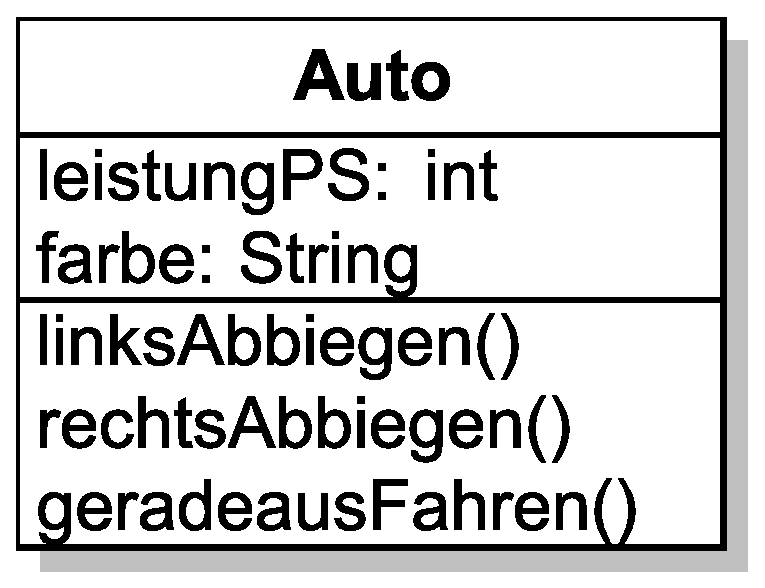
\includegraphics[width=0.2\textwidth]{./inf/SEKII/10_Java_Klassen/Auto.eps}
\end{center}

Das Diagramm einer Klasse ist in drei Abschnitte geteilt. In den obersten
Abschnitt wird der Name der Klasse geschrieben.

In den mittleren Abschnitt trägt man die Eigenschaften der Klasse ein, die für
das Programm, das generiert werden soll, von Bedeutung sind. Die Eigenschaften
bezeichnet man als Attribute. Wenn man die Klasse programmiert, wird für jedes
Attribut eine Variable angelegt. Der Datentyp der Variablen steht durch einen
Doppelpunkt getrennt hinter dem Namen des Attributs.

In den unteren Abschnitt schreibt man die Methoden, die auf die Objekte der
Klasse angewendet werden können.

In der Programmiersprache Java beschreibt eine Klasse das gemeinsame Schema für
alle ihre Objekte. Der Code wird nur einmal programmiert und automatisch auf
jedes Objekt angewendet, das zu der Klasse gehört.


\section{Beispiel: Klasse Hund}

\begin{minipage}{0.5\textwidth}
\begin{center}
\includegraphics[width=0.66\textwidth]{./inf/SEKII/10_Java_Klassen/HundVorversion.eps}
\end{center}
\end{minipage}
\begin{minipage}{0.5\textwidth}
\subsubsection{Sichtbarkeit}

\lstinline|private| (-) : Variable/Methode kann
nicht von anderer Klasse aufgerufen
werden.

\lstinline|public| (+) : Variable/Methode kann
von jeder anderen Klasse aufgerufen
werden.
\end{minipage}

\subsection{Eine erste Version der Klasse Hund}

(Datei \myFile{HundVorversion.java} im Kurs-Repository)

\begin{lstlisting}
import java.awt.*;

public class Hund {
  public Color farbe = Color.LIGHT_GRAY;
  public boolean wedeln = false;
  public int x = 0;       æ// x- und y-Koordinate der
æ  public int y = 0;       æ// linken oberen Ecke
  // Klassenvariable: zählt die Anzahl aller Hunde - aber wann???
æ  static private int anzahl = 0;

  public void stehen(Graphics g) {     æ// malt den Hund stehend
æ    malen(g, true);
  }

  public void springen(Graphics g) {   æ// malt den Hund springend
æ    malen(g, false);
  }
  
  æ// "interne" Programmierung: malen() ist aus anderen Klassen heraus nicht sichtbar!
æ  private void malen(Graphics g, boolean stehen) {
    Color c = g.getColor();
    if (wedeln) {
      g.drawLine(x+0,y+0,x+10,y+20);
    } else {
      g.drawLine(x+0,y+40,x+10, y+20);
    }
    if (stehen) {
      g.drawLine(x+18, y+40, x+18, y+60);
      g.drawLine(x+20, y+40, x+20, y+60);
      g.drawLine(x+44, y+40, x+44, y+60);
      g.drawLine(x+46, y+40, x+46, y+60);
    } else {
      g.drawLine(x+18, y+40, x+0, y+52);
      g.drawLine(x+20, y+40, x+2, y+52);
      g.drawLine(x+44, y+40, x+56, y+52);
      g.drawLine(x+46, y+40, x+58, y+52);
    }
    g.setColor(farbe);
    g.fillRoundRect(x+10, y+15, 45, 25, 12, 12);
    g.fillOval(x+49,y+0,21,21);
    g.setColor(c);
    g.drawRoundRect(x+10, y+15, 45, 25, 12, 12);
    g.drawOval(x+49,y+0,21,21);
  }
}
\end{lstlisting}


\subsubsection{Was bedeutet static?}

Alle normalen (nicht \lstinline|static|) Variablen und Methoden beziehen sich
immer auf ein spezielles Objekt, dessen Namen man angeben muss.

\lstinline|static| Variable: Es gibt die Variable nur einmal pro Klasse.

\lstinline|static| Methode: Die Methode bezieht sich nicht auf ein einzelnes
Objekt und darf keine Objekt-Variablen verwenden.


Um Objekte der Klasse \myClass{Hund} in einem eigenen Programm zu nutzen würde
man jetzt wie folgt vorgehen. Zunächst würde man eine Variable vom Typ \myClass{Hund}
deklarieren:

\begin{lstlisting}
Hund felix;
\end{lstlisting}

Anschließend könnte man ein entsprechendes \myClass{Hund}-Objekt erzeugen:

\begin{lstlisting}
felix = new Hund();
\end{lstlisting}

Dazu wurde der sogenannte \emph{Konstruktor} der Klasse mit dem
\lstinline|new|-Operator aufgerufen. Ein Konstruktor hätte in der Klasse
\myClass{Hund} programmiert werden können. Aber in der ersten Version der Klasse
\myClass{Hund} ist davon nichts zu sehen.

Tatsächlich \emph{muss} man keinen Konstruktor programmieren. In diesem Fall
gibt es immer einen parameterlosen Konstruktor, der ein neues Objekt der Klasse
erzeugt. Dabei werden alle Objektvariablen so initialisiert, wie es in der
Klasse vorgegeben ist.

Das Hund-Objekt \lstinline|felix| hätte somit zu Beginn folgende Attributwerte:

\begin{tabular}{ll}
\lstinline|farbe| & \lstinline|Color.LIGHT_GRAY| \\
\lstinline|wedeln| \hspace{5mm} & \lstinline|false| \\
\lstinline|x| & \lstinline|0| \\
\lstinline|y| & \lstinline|0| \\
\end{tabular}

Da diese Attribute alle als \lstinline|public| deklariert wurden, lassen sich
diese Werte nun aus der Anwendungsklasse heraus problemlos ändern:

\begin{lstlisting}
felix.x = 100;
felix.y = 250;
felix.farbe = Color.BLACK;
felix.wedeln = true;
\end{lstlisting}

Um unser Hund-Objekt nun im Anwendungsprogramm auch sehen zu können, müssen wir
noch eine der beiden Methoden \lstinline|springen()| oder \lstinline|stehen()|
benutzen:

\begin{lstlisting}
felix.stehen(g);
\end{lstlisting}

Der \myClass{Graphics}-Kontext, den wir in \lstinline|myPaint()| automatisch
haben, ist der benötigte Parameter \lstinline|g|. Die Methoden zum Zeichnen der
Objekte werden also immer innerhalb von \lstinline|myPaint()| aufgerufen (bzw.
in Methoden, die ihrerseits in \lstinline|myPaint()| aufgerufen wurden und den
\myClass{Graphics}-Kontext als Parameter mit übernommen haben).

So weit so gut. Spätestens wenn du eine Hand voll Hunde erzeugt und mit
individuellen Attributwerten ausgestattet hast, wirst du dir jedoch eine
bequemere Methode zum Erzeugen von solchen Objekten wünschen. Wenn dir das nicht
sofort einleuchtet, dann solltest du es ausprobieren!


\subsection{Klasse Hund mit selbstdefinierten Konstruktoren}

Die Lösung besteht darin einen (oder auch mehrere!) Konstruktor in der Klasse
\myClass{Hund} zu programmieren (Datei \myFile{Hund.java} im Kurs-Repository).

Konstruktoren erkennst du daran, dass sie exakt den selben Namen wie die Klasse
tragen (und deshalb im Unterschied zu normalen Methoden auch mit einem
Großbuchstaben beginnen). Außerdem haben sie keinen Rückgabewert. Nicht einmal
das Schlüsselwort \lstinline|void|, welches normalerweise verwendet wird um bei
Methoden anzugeben, dass sie keinen Rückgabewert liefern, wird hier benutzt!

Wenn -- wie in unserem Beispiel hier -- mehrere Konstruktoren programmiert
werden, dann müssen sich diese anhand der Datentypen der Parameterliste
unterscheiden lassen. So kann es beispielsweise nicht zwei verschiedene
Konstruktoren in der selben Klasse geben, die beide als Parameter zwei Integer
Werte erwarten. Anhand der unterschiedlichen Parameterlisten kann der
Java-Compiler dann entscheiden, welcher der vorhandenen Konstruktoren im
konkreten Fall zu benutzen ist.

In unserer Klasse \myClass{Hund} werden vier Konstruktoren definiert. Wenn man
sich die Datentypen der Parameterlisten dieser vier Konstruktoren ansieht,
erkennt man, dass diese eindeutig voneinander unterscheidbar sind:

Liste der Konstruktoren der Klasse \myClass{Hund}:

\begin{tabular}{l}
\lstinline|Hund()| \\
\lstinline|Hund(int, int, Color)| \\
\lstinline|Hund(int, int, boolean)| \\
\lstinline|Hund(Color, boolean)| \\
\end{tabular}

\vspace{1mm}

\begin{lstlisting}
import java.awt.*;

public class Hund {
  public Color farbe = Color.LIGHT_GRAY;
  public boolean wedeln = false;
  public int x = 0;       æ// x- und y-Koordinate der
æ  public int y = 0;       æ// linken oberen Ecke
æ  static private int anzahl = 0; æ// Klassenvariable: Anzahl aller Hunde
æ
  public Hund() {
    wedeln = true;
    anzahl++;
  }

  public Hund(int xPos, int yPos, Color farbe) {
    x = xPos;
    y = yPos;
    this.farbe = farbe;
    wedeln = true;
    anzahl++;
  }

  public Hund(int x, int y, boolean wedeln) {
    this.x = x;
    this.y = y;
    farbe = Color.YELLOW;
    this.wedeln = wedeln;
    anzahl++;
  }

  public Hund(Color f, boolean w) {
    farbe = f;
    wedeln = w;
    anzahl++;
  }

  static public int getAnzahlHunde() {
    return anzahl;
  }

  public void stehen(Graphics g) {      æ// malt den Hund stehend
æ    malen (g, true);
  }
  
  public void springen (Graphics g) {   æ// malt den Hund springend
æ    malen (g, false);
  }

  private void malen (Graphics g, boolean stehen) {
    ...
  }
}
\end{lstlisting}


\section{Objekte erzeugen}

Eine Klasse gibt das Schema für eine Gruppe gleichartiger Objekte vor. Ein
konkret existierendes Objekt bezeichnet man auch als Instanz.

Zum Erzeugen eines Objektes (bzw. einer Instanz) einer Klasse muss man zunächst
eine Variable mit dem Typ der Klasse deklarieren, zum Beispiel:

\begin{lstlisting}
Hund hund1;
\end{lstlisting}

Schema:

\begin{lstlisting}
Klasse variablenname;
\end{lstlisting}

Diese Variable selbst enthält jedoch noch kein Objekt. Die Variable dient dazu
die Speicheradresse abzuspeichern, an der sich die Daten des Objektes im
Hauptspeicher befinden. Solange die Variable noch nicht auf ein Objekt zeigt,
hat sie den Wert \lstinline|null|. \lstinline|null| bedeutet „kein Objekt“.

Das Anlegen eines Objektes und das Abspeichern der Speicheradresse in der
Variablen geschieht zum Beispiel mit folgenden Befehlen:

\begin{lstlisting}
hund1 = new Hund();
hund2 = new Hund(50, 50, Color.YELLOW);
\end{lstlisting}

Schema:

\begin{lstlisting}
Variablename = new Klasse(Parameter);
\end{lstlisting}

Man kann die Deklaration und das Erzeugen des Objektes auch in einem Befehl
zusammen fassen:

\begin{lstlisting}
Hund hund1 = new Hund();
\end{lstlisting}

Wenn es für das Programm nützlich ist, kann man weitere Variablen auf dasselbe
Objekt zeigen lassen:

\begin{lstlisting}
Hund hilfe = hund1;   æ// hilfe zeigt auch auf hund1
\end{lstlisting}

Ein Objekt lebt solange, wie es Variablen gibt, die auf das Objekt verweisen.
Sobald es auf ein Objekt keinen Verweis mehr gibt, wird das Objekt vom System
automatisch vernichtet. Wenn man explizit sagen möchte, dass eine Variable auf
kein Objekt zugreift, so kann man ihr den Wert \lstinline|null| zuweisen:

\begin{lstlisting}
hund1 = null;
\end{lstlisting}


\section{Variablen einer Klasse}

Es gibt drei verschiedene Arten von Variablen, die in dem folgenden Beispiel
verdeutlicht werden:

\begin{lstlisting}
class Beispiel {
  static int klassenVariable;   æ// 1 mal pro Klasse
æ  int objektVariable;           æ// 1 mal pro Objekt
æ
  void methode() {
    int lokaleVariable;         æ// nur innerhalb von methode()
æ  }
}
\end{lstlisting}

\textbf{Klassenvariablen} beziehen sich auf alle Objekte der Klasse und sind
deshalb nur einmal vorhanden. Beispiel: Ein Zähler, der zählt, wie viele Objekte
der Klasse angelegt werden.

\textbf{Objektvariablen} speichern die Daten eines speziellen Objektes, z.B.\
die Farbe eines Hundes. Jedes Objekt besitzt seine eigenen Objektvariablen.

\textbf{Lokale Variablen} werden innerhalb einer Methode deklariert und werden
am Ende der Methode automatisch vom System wieder gelöscht.

Klassen- und Objektvariablen werden vom System automatisch mit \lstinline|0|
bzw.\ \lstinline|false| oder \lstinline|""| (leerer String) initialisiert.
Lokale Variablen dagegen haben zu Beginn einen unbestimmten Wert.


\subsection{Zugriff auf Variablen}

\begin{compactenum}[a)]
\item von außen

Von außen (d.h.\ von einer anderen Klasse aus) greift man auf Klassenvariablen
nach folgendem Schema zu:

\begin{lstlisting}
Klasse.attribut
\end{lstlisting}

Beispiel:

\begin{lstlisting}
Beispiel.klassenVariable = 10;
\end{lstlisting}

Auf eine Objektvariable kann man nur dann zugreifen, wenn man ein Objekt
besitzt. Schema:

\begin{lstlisting}
objekt.attribut
\end{lstlisting}

Beispiel:

\begin{lstlisting}
Beispiel bsp = new Beispiel();
bsp.objektVariable = 5;
\end{lstlisting}

\item innerhalb einer Klasse

Innerhalb einer Klasse kann man auf alle Klassen und Objektvariablen direkt
zugreifen ohne vorher den Klassen- oder Objektnamen anzugeben. Tatsächlich kann
man gar keinen „richtigen“ Objektnamen angeben, da die Klasse ja den Code für
alle Objekte darstellt. Um eine Objektvariable direkt anzusprechen (z.B. um sie
von einer lokalen Variablen mit dem gleichen Namen zu unterscheiden), kann man
das Objekt \lstinline|this| verwenden. \lstinline|this| bezeichnet das aktuelle
Objekt (analog zu dem menschlichen Ausdruck „ich“). In der Klasse Beispiel
könnte beispielsweise stehen:

\begin{lstlisting}
this.objektVariable = 10;
\end{lstlisting}
\end{compactenum}


\section{Methoden}

Methoden, die mit dem Schlüsselwort \lstinline|static| gekennzeichnet sind,
können jederzeit auch ohne Existenz eines Objektes aufgerufen werden. Sie
dürfen jedoch nur Klassenvariablen und lokale Variablen verwenden.

Alle nicht statischen Methoden, werden immer auf ein Objekt der Klasse
angewendet. Mit ihnen kann man die Objektvariablen des aktuellen Objektes
verändern.


\section{Konstruktor}

Der Konstruktor ist eine spezielle Methode, die vom System bei der Erzeugung
eines Objektes mit dem \lstinline|new| Operator aufgerufen wird. Er ist dazu
gedacht, Initialisierungen für das Objekt vorzunehmen (also Anfangswerte für
die Variablen des Objektes zu setzen). Das besondere:

\begin{compactitem}
\item Der Methodenname des Konstruktors ist mit dem Namen der Klasse identisch
\item Der Konstruktor besitzt keinen Rückgabewert (auch nicht
\lstinline|void|!). Aber er kann beliebig viele Parameter besitzen.
\item Der Konstruktor darf niemals explizit aus einer anderen Methode heraus
aufgerufen werden.
\end{compactitem}
  \section{Animationen erzeugen}

Mit Hilfe der Klasse \myClass{javax.swing.Timer} kann man dafür sorgen, dass
die \lstinline|myPaint()|-Routine in regelmäßigen Abständen immer wieder
aufgerufen wird.

Dies ermöglicht es einfache Animationen zu schreiben, indem man eine Figur, wie
z.B. einen Ball, bei jedem neuen Aufruf von \lstinline|myPaint()| an einer
anderen Position malt. Es entsteht dann der Eindruck einer Bewegung.
Die Klasse \myClass{Timer} besitzt die folgenden Methoden:

\bgroup
\def\arraystretch{1.2}
\begin{tabular}{|l|p{75mm}|}
\hline
\lstinline|Timer(int millisec, ActionListener frame)| &
Über den Konstruktor wird dem Timer mitgeteilt, in welchem zeitlichen Abstand
ein ActionEvent erzeugt werden soll. Der zweite Parameter benennt die Anwendung
die auf den Event reagieren soll. In der Klasse \myClass{HJFrame} ist dies
bereits fertig implementiert, so dass bei jedem so empfangenen ActionEvent das
Fenster neu gezeichnet wird. Als zweiter Parameter wird deshalb von euch
typischerweise \lstinline|this| verwendet.
\\ \hline
\lstinline|void start()| & 
Mit dieser Methode wird der Timer gestartet.
\\ \hline
\lstinline|void stop()| &
Durch Aufruf der Methode \lstinline|stop()| wird der wiederholte Aufruf der
\lstinline|myPaint()|-Methode beendet. Nachdem \lstinline|stop()| aufgerufen
wurde, ist ein erneuter Start möglich.
\\ \hline
\end{tabular}
\egroup

\subsection{Beispiel für eine Animation}

Du findest die Datei \myFile{Animation.java} im Kurs-Repository.

\begin{lstlisting}
æimport java.awt.Color;
import java.awt.EventQueue;
import java.awt.Graphics;æ
import javax.swing.Timer;æ
import hilfe.*;

public class Animation extends HJFrame {
  // globale Variablen
  private static final int WIDTH = 500;
  private static final int HEIGHT = 500;
  private static final Color BACKGROUND = Color.WHITE;
  private static final Color FOREGROUND = Color.BLACK;æ
  private int zaehler = 0;æ

  public Animation(final String title) {
    super(WIDTH, HEIGHT, BACKGROUND, FOREGROUND, title);
    // eigene Initialisierung
æ    Timer timer = new Timer(10, this);
    timer.start();æ
  }
  
  @Override
  public void myPaint(Graphics g) {
    // wird aufgerufen, wenn das Fenster neu gezeichnet wird
æ    zaehler++;æ
    g.drawLine(0, 0, æzaehleræ, æzaehleræ);
    g.drawLine(WIDTH, HEIGHT, WIDTH-æzaehleræ, HEIGHT-æzaehleræ);
    g.drawLine(0, HEIGHT, æzaehleræ, HEIGHT-æzaehleræ);
    g.drawLine(WIDTH, 0, WIDTH-æzaehleræ, æzaehleræ);
  }
  
  public static void main(final String[] args) {
    EventQueue.invokeLater(new Runnable() {
      public void run() {
        try {
          Animation anwendung = new Animation("Animation");
        } catch (Exception e) {
          e.printStackTrace();
        }
      }
    });
  }
}
\end{lstlisting}


\section{Klassen aus dem Package hilfe}

Das Package \myPackage{hilfe} enthält neben der Klasse \myClass{HJFrame} weitere
Vereinfachungen für Programmieraufgaben, die für euch mit den
Standard-Java-Klassen aus dem JRE im Moment noch zu schwer zu programmieren
sind. Damit Klassen aus dem Package \myPackage{hilfe} verwendet werden können,
muss am Anfang einer Java-Datei folgende \lstinline|import|-Anweisung eingefügt
werden:

\begin{lstlisting}
import hilfe.*;
\end{lstlisting}

\subsection{Zeichnen von Dreiecken}

Zum Zeichnen von Dreiecken steht die Klasse \myClass{HZeichnen} zur Verfügung,
die folgende Methoden besitzt:

\begin{compactitem}
\item
\lstinline|static void drawDreieck(Graphics g, int x1, int y1, int x2, int y2, int x3, int y3)| 

\lstinline|drawDreick()| malt ein hohles Dreieck mit den drei Eckpunkten (x1,
y1), (x2, y2) und (x3, y3). Als erster Parameter muss ein Objekt der
Klasse \myClass{Graphics} übergeben werden, da die Methode dieses Objekt zum
Malen braucht.
\item
\lstinline|static void fillDreieck(Graphics g, int x1, int y1, int x2, int y2, int x3, int y3)|

\lstinline|fillDreick()| malt ein gefülltes Dreieck mit den drei Eckpunkten (x1,
y1), (x2, y2) und (x3, y3).
\end{compactitem}

Beispiel für die Verwendung der \lstinline|fillDreieck()|-Methode:

\begin{lstlisting}
HZeichnen.fillDreieck(g, 10, 90, 50, 90, 30, 60);
\end{lstlisting}

  \clearpage

\lehead[]{\sf\hspace*{-2.00cm}\textcolor{white}{\colorbox{lightblue}{\parbox[c][0.70cm][b]{1.60cm}{
\makebox[1.60cm][r]{\thechapter}\\ \makebox[1.60cm][r]{ÜBUNG}}}}\hspace{0.17cm}\textcolor{lightblue}{\chaptertitle}}
\rohead[]{\textcolor{lightblue}{\chaptertitle}\sf\hspace*{0.17cm}\textcolor{white}{\colorbox{lightblue}{\parbox[c][0.70cm][b]{1.60cm}{\thechapter\\
ÜBUNG}}}\hspace{-2.00cm}}
%\chead[]{}
\rehead[]{\textcolor{lightblue}{AvHG, Inf, My}}
\lohead[]{\textcolor{lightblue}{AvHG, Inf, My}}

\section{Klassen und Objekte -- Übungen}

\subsection{Aufgabe 1: Hunde}

\begin{compactenum}[a)]
\item Erzeuge mindestens vier verschiedene Objekte der Klasse \myClass{Hund} und
zeichne sie entweder stehend oder springend im Frame. Jeder Hund soll nur an
einer Position gemalt werden, denn schließlich sieht man ja auch einen Hund in
der realen Welt nicht doppelt (es sei denn man hat zuviel getrunken). Gib
außerdem die Anzahl der Hunde im Frame aus. Benutze hierfür die statische
Methode \lstinline|getAnzahlHunde()|.

\item Programmiere einen der Hunde so, dass er bei jedem neuen Aufruf der
Methode \lstinline|myPaint()| abwechselnd den Schwanz senkt oder hebt.

\item Benutze ein Objekt der Klasse \myClass{Timer} um dafür zu sorgen, dass
\lstinline|myPaint()| in regelmäßigen Abständen aufgerufen wird. Nun sollte der
in b) programmierte Hund intensiv wedeln.

\item Lass einen der Hunde von links nach rechts über den Bildschirm laufen.
Wenn er rechts aus dem Bild herausgelaufen ist, soll er wieder von links in das
Bild hinein laufen. Damit der Lauf möglichst realistisch wirkt, soll der Hund
abwechselnd in stehender und in springender Position gezeichnet werden.
\end{compactenum}


\subsection{Aufgabe 2: Raupe}

\begin{compactenum}[a)]
\item Erzeuge eine neue, leere Datei (kein Anwendungsfenster!!!) und
programmiere in der Datei die Klasse \myClass{Raupe}. Eine Raupe besitzt zu
Anfang die Attribute x-Position, y-Position, Farbe und Geschwindigkeit in
x-Richtung. Alle Attribute sollen \lstinline|private| sein.

Die Startwerte für die vier Attribute werden im Konstruktor als
Parameter übergeben.

Schreibe eine Methode \lstinline|zeichnen()|, die die Raupe an ihrer aktuellen
Position in der für sie gewählten Farbe zeichnet. Die Raupe soll durch zwei
ausgefüllte Kreise und ein ausgefülltes Rechteck dargestellt werden. Das Kreuz
markiert die linke obere Ecke, die durch den x- und y-Wert beschrieben wird (1
Kästchen entspricht 10 Pixeln):

\begin{center}
\includegraphics[width=0.3\textwidth]{./inf/SEKII/10_Java_Klassen/raupe_lang.png}
\end{center}

\item Programmiere ein Anwendungsfenster und erzeuge im Anwendungsfenster
mehrere Raupen-Objekte mit unterschiedlichen Attributen und zeichne sie in der
Methode \lstinline|myPaint()|.

\item Erzeuge im Anwendungsfenster ein Objekt der Klasse \myClass{Timer}, damit
die Methode \lstinline|myPaint()| wiederholt aufgerufen wird.

\item Die Raupe soll sich wiederholt von links nach rechts über den Bildschirm
bewegen. Programmiere dazu in der Klasse \myClass{Raupe} eine parameterlose
Methode \lstinline|bewegen()|, die die x-Position der Raupe entsprechend ihrer
Geschwindigkeit nach rechts verschiebt. Nachdem die Raupe aus dem Bild
„gelaufen“ ist, soll ihre neue x-Position so gewählt werden, dass sie langsam
in das Bild hinein gleitet.

Rufe im Anwendungsfenster in der Methode \lstinline|myPaint()| die Methode
\lstinline|bewegen()| für jede Raupe auf.

\item Die Laufbewegung einer Raupe soll auf einfache Weise simuliert werden, in
dem die Raupe ihre Größe verändert.

\begin{compactitem}
\item Leichte Variante: Die Raupe soll immer abwechselnd einmal mit normaler
Länge gezeichnet werden und beim nächsten Mal wie abgebildet verkürzt
dargestellt werden.
\item Schwere Variante: Die Raupe soll immer abwechselnd drei mal hintereinander
mit normaler Länge gezeichnet werden und dann drei mal hintereinander auf
folgende Weise verkürzt dargestellt werden:

\begin{center}
\includegraphics[width=0.32\textwidth]{./inf/SEKII/10_Java_Klassen/raupe_kurz.png}
\end{center}

\end{compactitem}

\end{compactenum}


\subsection{Aufgabe 3: Strichmännchen}

\begin{compactenum}[a)]
\item Überlege dir, welche Attribute die Klasse \myClass{Strichmaennchen}
besitzen muss. Damit es nicht zu langweilig wird, sollen sich die Objekte der
Klasse \myClass{Strichmaennchen} in folgenden Eigenschaften unterscheiden:

\begin{minipage}{0.85\textwidth}
\begin{compactitem}
\item unterschiedliche Kleidung (Farbe)
\item Laufen in unterschiedlichen Geschwindigkeiten
\item unterschiedliche y-Positionen (einige Männchen laufen oben andere weiter
unten)
\end{compactitem}

Ein Strichmännchen soll zunächst zwei Methoden erhalten:

\begin{compactitem}
\item Eine Methode \lstinline|zeichnen()|, die ein Strichmännchen an seiner
aktuellen Position auf dem Bildschirm malt.
\item Eine Methode \lstinline|laufen()|, die ein Strichmännchen entsprechend
seiner aktuellen Geschwindigkeit eine Position nach vorne setzt.
\end{compactitem}
\end{minipage}
\begin{minipage}{0.15\textwidth}
\begin{center}
\includegraphics[width=0.4\textwidth]{./inf/SEKII/10_Java_Klassen/strichmaennchen.png}
\end{center}
\end{minipage}

\item Entwirf die Figur eines Strichmännchens auf kariertem Papier.

\item Programmiere die Klasse \myClass{Strichmaennchen} und erzeuge mehrere
Strichmännchen-Objekte, die über den Bildschirm laufen. Alle Strichmännchen
sollen unterschiedliche Attribut-Werte besitzen. Bei jedem Aufruf der
\lstinline|myPaint()|-Methode werden die Strichmännchen durch Aufruf der
Methode \lstinline|laufen()| um eine Position weiter nach rechts bewegt.
Anschließend werden sie durch Aufruf der Methode \lstinline|zeichnen()| an ihrer
aktuellen Position auf dem Bildschirm gemalt. Verwende die Klasse
\myClass{Timer}, damit die Methode \lstinline|myPaint()| in regelmäßigen
Abständen immer wieder aufgerufen wird.

\item Das Strichmännchen soll jetzt etwas lebendiger gestaltet werden, in dem
es zyklisch in verschiedenen Positionen oder mit verschiedenen Bildern gemalt
wird. Zum Beispiel könnte man vier verschiedene Bilder des Strichmännchens
entwerfen, bei denen die Arme und Beine sich jeweils in unterschiedlichen
Laufstellungen befinden. Wenn man diese Bilder dann der Reihe nach immer
wiederholt, entsteht für den Betrachter der Eindruck einer Bewegung.

\item Vermutlich habt ihr alle ein typisch europäisches Strichmännchen
gezeichnet. Ein großer Teil der Weltbevölkerung besteht aber aus Afrikanern,
Asiaten, usw.. Damit auch diese Personen zu ihrem „Strichmännchen-Recht“
kommen, wird die Klasse \myClass{Strichmaennchen} so abgewandelt, dass jedes
dritte Strichmännchen automatisch mit „fremdländischen“ Attributen versehen
wird, z.B. eine dunklere Hautfarbe. Dazu wird in der Klasse Strichmännchen ein
Zähler benötigt, der als Klassenvariable realisiert wird.
\end{compactenum}


\subsection{Aufgabe 4: Blumen}

\begin{compactenum}[a)]
\item Programmiere in einer neuen Datei eine Klasse \myClass{Blume}.

Eine Blume besitzt zu Anfang die Attribute x-Position, y-Position und Farbe.
Weitere Attribute dürfen später nach Bedarf hinzugefügt werden. Die Startwerte
für die x- und y-Position werden im Konstruktor als Parameter übergeben (in
dieser Reihenfolge). Die Farbe wird automatisch auf rot gestellt.

Schreibe eine Methode \lstinline|zeichnen()|, die die Blume an ihrer aktuellen
Position zeichnet. Das Kreuz markiert die linke obere Ecke, die durch den x-
und y-Wert beschrieben wird (1 Kästchen entspricht 10 Pixeln):

\begin{minipage}{0.5\textwidth}
\begin{center}
\includegraphics[width=0.2\textwidth]{./inf/SEKII/10_Java_Klassen/blumeBluehend.png}
\end{center}
\end{minipage}
\begin{minipage}{0.5\textwidth}
\begin{center}
\includegraphics[width=0.2\textwidth]{./inf/SEKII/10_Java_Klassen/blumeVerwelkt.png}
\end{center}
\end{minipage}

Anmerkung: Zu Beginn gibt es nur „blühende“ Blumen (linkes Bild). Die vier
äußeren Kreise werden in der eingestellten Blumen-Farbe ausgefüllt. Der
mittlere Kreis wird gelb gefüllt. Der Stängel wird als ausgefülltes, grünes
Rechteck mit drei Pixel Breite gezeichnet und geht von der Blume bis zum Boden
(also bis zum unteren Rand des Fensters). Der Einfachheit halber kann man den
Stängel auch über den Rand des Fensters hinaus zeichnen.

\item Erzeuge ein Anwendungsfenster mit mindestens sechs Blumen-Objekten. Füge
außerdem in das Anwendungsfenster ein Objekt der Klasse \myClass{Timer} ein.

\item Erweitere die Methode \lstinline|zeichnen()| so, dass die Blume bei jedem
Aufruf um ein Pixel wächst bis sie die y-Position 100 erreicht hat. Das heißt
die y-Position wird immer um ein Pixel nach oben verschoben bis die angegebene
Höhe erreicht ist.

\item Sorge im Konstruktor dafür, dass die Blumen automatisch unterschiedliche
Farben erhalten und zwar immer abwechselnd \lstinline|Color.RED|,
\lstinline|Color.BLUE| oder \lstinline|Color.CYAN|. Die erste und die vierte
Blume müssen also rot werden. Die zweite und die fünfte Blumen werden blau und
die dritte und die sechste Blume werden cyan. Selbstverständlich muss der Code
so geschrieben sein, dass er auch für weitere Blumenobjekte funktioniert.

\item Jede Blume verwelkt zwei Sekunden nachdem sie ihre maximale Höhe erreicht
hat und wird dann wie oben rechts abgebildet gezeichnet.
\end{compactenum}


\subsection{Aufgabe 5: Verhältnis von Klassen und Objekten}

Erkläre die Begriffe Klasse und Objekt anhand der folgenden Worte: Hund, Hasso,
Lassie, Katze, Miezi.


\subsection{Aufgabe 6: Fachbegriffe} 

Finde jeweils das richtige Fachwort.

\bgroup
\def\arraystretch{1.2}
\begin{tabular}{|l|p{65mm}|}
\hline
Festlegung von Namen und Datentyp für eine Variable & \\ \hline
Art einer Variable & \\ \hline
Variable, die im Kopf einer Methode deklariert wird & \\ \hline
Anfangswert für eine Variable setzen & \\ \hline
Wiederholungsanweisung & \\ \hline
Eigenschaft, die ein Objekt einer Klasse beschreibt & \\ \hline
Tätigkeit, die Objekte einer Klasse ausführen können & \\ \hline
\end{tabular}
\egroup


\subsection{Aufgabe 7: Variablendeklaration}

\begin{compactenum}[a)]
\item Wie deklariert man eine Variable in Java?
\item Welches Schlüsselwort muss vor einer Variablendeklaration stehen, wenn
eine Variable \ldots 

\bgroup
\def\arraystretch{1.2}
\begin{tabular}{|l|p{45mm}|}
\hline
\ldots nicht verändert werden darf (also konstant ist) & \\ \hline
\ldots von einer anderen Klasse benutzt werden darf. & \\ \hline
\ldots von einer anderen Klasse nicht benutzt werden darf. & \\ \hline
\ldots nur einmal pro Klasse vorhanden ist (also nicht für jedes Objekt). & 
\\ \hline
\end{tabular}
\egroup
\end{compactenum}


\subsection{Aufgabe 8: Entwurf einer Methode (1)}

Programmiere auf Papier eine Methode \lstinline|treffer()|, die eine
Fließkommazahl als Parameter erhält und einen booleschen Wert zurück gibt. Es
wird der Wert \lstinline|true| zurückgegeben, wenn eine der Zahlen
\lstinline|1.5|, \lstinline|4| oder \lstinline|5.5| angegeben wird. Andernfalls
wird der Wert \lstinline|false| zurück gegeben.


\subsection{Aufgabe 9: Entwurf einer Methode (2)}

Programmiere auf Papier eine Methode \lstinline|summe()|, die eine ganze Zahl
\lstinline|x| als Parameter erhält und eine (eventuell sehr große) ganze Zahl
als Rückgabewert zurück gibt. Die Methode soll alle ganzen Zahlen von zehn bis zu
der übergebenen Zahl \lstinline|x| aufaddieren.


\subsection{Aufgabe 10: Programmierung von Klassen und Objekten}

\begin{compactenum}[a)]
\item Mit welchem Schlüsselwort kennzeichnet man beim Programmieren eine
Klasse?
\item Angenommen es existiert eine Klasse \myClass{Fisch}. Wie erzeugt man im
Anwendungsfenster eine Variable, die auf ein Objekt dieser Klasse verweisen
kann?
\item Wie erzeugt man ein neues Objekt der Klasse im Speicher?
\item Wann wird das Objekt wieder aus dem Speicher gelöscht?
\end{compactenum}


\subsection{Aufgabe 11: Verweis auf sich selbst}

Eine Klasse beschreibt das Schema für eine ganze Gruppe von Objekten. Wie
verweist man beim Programmieren innerhalb der Klasse auf das eigene Objekt
(also quasi auf sich selber)? 


\subsection{Aufgabe 12: Konstruktor}

\begin{compactenum}[a)]
\item Was ist ein Konstruktor?
\item Wann wird der Konstruktor einer Klasse aufgerufen?
\item Wie programmiert man einen Konstruktor?
\end{compactenum}


\subsection{Aufgabe 13: Leseübung}

Lies den folgenden Programmtext sorgfältig und beantworte die unten gestellten
Fragen.

\begin{lstlisting}
class Demo {
  public String name = "Demo";
  public double gewicht = 55.5;
  public int groesse;
  public static int alter;

  public Demo(String name, double gewicht) {
    this.name = name;
    gewicht = 87.2;
    alter = 50;
  }

  public Demo(String name, int a) {
    this.name = name;
    groesse = 183;
    alter = a;
  }

  public void drucken() {
    // Ausgabe der Daten eines Objektes auf die Konsole
    System.out.println("Name: "+name);
    System.out.println("Gewicht: "+gewicht);
    System.out.println("Groesse: "+groesse);
    System.out.println("Alter: "+alter);
    System.out.println(" ---");
  }

  public static void main(final String[] args) {
    Demo a = new Demo("Mona", 51.3);
    Demo b;
    Demo c = a;
    Demo d = new Demo ("Simson", 19);
    c.gewicht = 45.0;
    a.drucken();
    c.drucken();
    d.drucken();
  }
}
\end{lstlisting}

\begin{compactenum}[a)]
\item Markiere im Code die Deklaration einer Klassenvariablen (K), einer
Objektvariablen (O) und einer lokalen Variablen (L).
\item Welche Methoden können benutzt werden, ohne dass es ein Objekt gibt?
\item Ermittle, welche Ausgabe das folgende Programm erzeugt. Zeichne dazu den
Inhalt der Objekte und Variablen im Hauptspeicher auf, um den Ablauf des
Programms nachzuvollziehen.
\item Was passiert wenn man \lstinline|b.drucken();| aufruft?
\item Was passiert bei der Anweisung: \lstinline|b = new Demo();| ?
\end{compactenum}

Hinweis: Du findest die Datei \myFile{Demo.java} im Kurs-Repository. Du solltest
die Aufgaben aber zunächst wirklich beantworten, ohne das Programm in Eclipse
auszuführen. Das kannst du dann anschließend tun um deine eigenen Antworten zu
überprüfen.


\subsection{Aufgabe 14: Autorennen}

\begin{compactenum}[a)]
\item Programmiere in einer neuen Datei eine Klasse \myClass{Auto}.

\item Ein Auto besitzt zu Beginn die Attribute x-Position, y-Position und
Farbe. Weitere Attribute dürfen später nach Bedarf hinzugefügt werden. Die
Startwerte für den y-Wert und die Farbe werden im Konstruktor als Parameter
übergeben (in der angegebenen Reihenfolge). Die x-Position wird automatisch auf
den Wert 10 gesetzt.

Schreibe eine Methode \lstinline|zeichnen()| (mit dem \myClass{Graphics}-Objekt
als Parameter), die das Auto an seiner aktuellen Position wie abgebildet
zeichnet. Zunächst werden zwei große ausgefüllte Rechtecke in der eingestellten
Autofarbe gezeichnet. Anschließend werden die Fenster mit zwei ausgefüllten
gelben Quadraten darüber gemalt. Danach wird der Bereich für den Auspuff und
die Räder schwarz ausgefüllt. Das Kreuz markiert die linke obere Ecke, die durch
den x- und y-Wert beschrieben wird. Ein Kästchen in der Abbildung entspricht
zehn Pixeln:

\begin{center}
\includegraphics[width=0.25\textwidth]{./inf/SEKII/10_Java_Klassen/auto.jpg}
\end{center}

\item Erzeuge ein Anwendungsfenster mit einer Breite von 800 Pixeln und einer
Höhe von 500 Pixeln. Zeichne im Anwendungsfenster mehrere Objekte der Klasse
\myClass{Auto}. Füge auch ein Objekt der Klasse \myClass{Timer} ein, das die
\lstinline|myPaint()|-Methode im Abstand von 100 Millisekunden wiederholt
aufruft.

\item Die Autos sollen sich nun bewegen. Füge dazu ein Attribut
\lstinline|speed| mit dem Datentyp \lstinline|int| in die Klasse ein, und setze
das Attribut im Konstruktor auf einen Zufallswert zwischen 5 und 14.

Um Zufallswerte erzeugen zu können, musst du in die Klasse \myClass{Auto} auch
noch eine Objekt der Klasse \myClass{Random} einfügen. Beachte, dass dieses
Objekt eine Klassenvariable sein muss, denn wenn jedes Auto seinen eigenen
Zufallsgenerator hätte, würden die meisten Autos exakt dieselbe Geschwindigkeit
erhalten, weil ihr Zufallsgenerator jeweils mit dem selben Anfangswert gestartet
wird.

Erweitere anschließend die Methode \lstinline|zeichnen()| so, dass die
x-Position des Autos bei jedem Aufruf um den Wert \lstinline|speed| nach rechts
verschoben wird. Wenn die x-Position größer als 800 ist, soll seine x- Position
links vor das Fenster gesetzt werden, so dass das Auto langsam in das Fenster
hinein gleitet.

\item Die Abgase des Autos sollen mit grau ausgefüllten Kreisen animiert
werden. Dazu werden vier Zustände unterschieden (durchnummeriert von 0 bis 3),
die das Auto der Reihe nach wiederholt durchläuft. Im Zustand 0 werden
keinerlei Abgase gezeichnet. Im Zustand 1 wird nur der mit 1 bezeichnete Kreis
gezeichnet. Im Zustand 2 werden die mit 1 und 2 bezeichneten Kreise gezeichnet.
Im Zustand drei werden alle drei Kreise gezeichnet.

\begin{center}
\includegraphics[width=0.3\textwidth]{./inf/SEKII/10_Java_Klassen/autoMitAbgasen.jpg}
\end{center}

\item Die Autos sollen in der Reihenfolge ihrer Erzeugung durchnummeriert
werden. Das erste Auto erhält die Nummer 1. Dazu musst du eine Klassenvariable
erzeugen, mit der die Autos im Konstruktor durchgezählt werden. Außerdem
benötigt man eine Objektvariable, in der jedes Auto seine eigene Nummer
abspeichert.

In der Methode \lstinline|zeichnen()| soll jedes Auto seine Nummer mit der
\myClass{Graphics}-Methode \lstinline|drawString()| an der Position (x+50, y+35)
mit schwarzer Schrift ausgeben.

\item Ein Autorennen dauert drei Runden. Nachdem ein Auto dreimal von links nach
rechts durch das Fenster gefahren ist, soll es nicht mehr gezeichnet werden.

Außerdem soll die Nummer des Autos, das als erstes „das Ziel“ erreicht, im
Anwendungsfenster an der Position (300, 480) mit einem kleinen Text ausgegeben
werden, z.B. „\myUserInput{Der Sieger ist Auto 4}“. Welche Klasse diese Ausgabe
übernimmt, darfst du selber entscheiden.
\end{compactenum}


\subsection{Aufgabe 15: Sternen-Himmel}

Es soll ein Sternen-Himmel programmiert werden.

\begin{compactenum}[a)]
\item Wähle im Anwendungsfenster-Fenster die Farbe schwarz als
Hintergrundfarbe aus.

\item Programmiere eine Klasse \myClass{Stern} mit folgenden Attributen:

\begin{compactitem}
\item der Farbe des Sterns
\item der linken oberen Ecke des Sterns (x- und y-Position)
\item der Geschwindigkeit des Sterns (Veränderung der x-Richtung in Pixel pro
Aufruf vom \lstinline|myPaint()|)
\end{compactitem}

Alle Attribute der Klasse dürfen von außen (d.h.\ von einer anderen Klasse aus)
nicht verändert werden. Weise den Variablen in der Klasse die entsprechende
Eigenschaft zu. Zur Programmierung der im nachfolgenden beschriebenen
Funktionalitäten dürfen weitere Klassen- und Instanzvariablen eingefügt werden.
Auch diese Variablen dürfen jedoch nicht von außen veränderbar sein.

Die Klasse Stern soll nur einen einzigen Konstruktor haben, in dem als
Parameter die x- und y- Position der linken oberen Ecke des Sterns angegeben
werden. Die Geschwindigkeit wird innerhalb des Konstruktors automatisch für
alle Sterne auf den Wert 3 gesetzt. Auch die Farbe wird automatisch generiert.
Jeder zweite Stern erhält die Farbe orange. Alle anderen Sterne erhalten die
Farbe gelb.

\vspace{1mm}

\begin{minipage}{0.85\textwidth}
Die Klasse Stern besitzt die öffentliche Methode \lstinline|zeichnen()|, die den
Stern an seiner aktuellen Position malt und ihn anschließend entsprechend der
eingestellten Geschwindigkeit in der x-Position verschiebt. Entscheide selbst, ob
die Methode \lstinline|zeichnen()| einen Parameter benötigt oder nicht. Ein
Stern wird durch zwei ausgefüllte Dreiecke gemalt, wie in der nebenstehenden
Abbildung zu sehen ist. Die linke obere Ecke, die durch die x- und y-Werte
beschrieben ist, ist im Bild durch einen dicken Punkt markiert. Dieser Punkt
soll natürlich nicht mit gezeichnet werden. Wähle beim Zeichnen pro Kästchen
eine Größe von 10 Pixel. Wenn ein Stern rechts aus dem Bild gewandert ist, soll
die Methode \lstinline|zeichnen()| ihn wieder auf der linken Seite ins Bild
setzen.
\end{minipage}
\begin{minipage}{0.15\textwidth}
\begin{center}
\includegraphics[width=0.5\textwidth]{./inf/SEKII/10_Java_Klassen/stern.png}
\end{center}
\end{minipage}

\vspace{1mm}

Damit ein Stern harmonisch in das Bild hinein gleitet, wird seine neue
x-Position nicht auf den Wert 0 gesetzt, sondern soweit nach links verschoben,
das zunächst nur seine rechten Spitzen sichtbar sind.

\item Erzeuge im Anwendungsfenster mindestens vier verschiedene Objekte der
Klasse \myClass{Stern} an verschiedenen Positionen. Sorge mit Hilfe der Klasse
\myClass{Timer} dafür, dass das Anwendungsfenster und die Sterne alle 100
Millisekunden neu gezeichnet werden.

\item Die Klasse \myClass{Stern} soll um das boolesche Attribut
\lstinline|blinkend| erweitert werden. Auch dieses Attribut darf von außen nicht
verändert werden. Der Standard-Wert für das Attribut ist \lstinline|false|
(ausgeschaltet).

Füge in die Klasse einen zweiten Konstruktor ein, mit dem neben der x- und
y-Position der Wert des Attributs \lstinline|blinkend| eingestellt werden kann.
Wenn \lstinline|blinkend| auf \lstinline|true| gesetzt wird, wird das Objekt nur
bei jedem zweiten Aufruf der Methode \lstinline|zeichnen()| tatsächlich
gezeichnet, so dass ein Blink-Effekt entsteht. 

Erzeuge im Anwendungsfenster ein weiteres Objekt der Klasse \myClass{Stern}, bei
dem das Attribut \lstinline|blinkend| eingeschaltet ist.

\item Hin und wieder ziehen am Himmel Wolken vorbei und verdecken die Sterne.
Wenn eine Wolke da ist, sind alle Sterne nicht sichtbar und werden daher nicht
gezeichnet. Ergänze die Klasse \myClass{Stern} um ein öffentliches boolesches
Attribut \lstinline|wolke_da|, das nur einmal für die gesamte Klasse existieren
soll.
Wenn eine Wolke vorhanden ist, werden die Sterne in der Methode
\lstinline|zeichnen()| nicht gezeichnet. Achte darauf, dass der Wolken-Effekt
auch für blinkende Sterne korrekt funktioniert.

Stelle das boolesche Attribut \lstinline|wolke_da| des Anwendungsfensters so
ein, dass immer abwechselnd 1200 ms lang keine Wolke da ist und dann 600 ms
lang eine Wolke vorüber zieht.
\end{compactenum}


\subsection{Aufgabe 16: Bälle (alte Klausuraufgabe)}

\emph{Hinweis: In kursiver Schrift wird bei einigen Teilaufgaben eine
Alternative für diejenigen vorgeschlagen, die Probleme haben, die Teilaufgabe
zu lösen. Der Alternativ-Vorschlag soll euch dazu befähigen, mit den anderen
Teilaufgaben weiterzumachen, damit ihr euch nicht an einem Problem fest beißt.
Wer den Alternativ- Vorschlag wählt, erhält für die jeweilige Teilaufgabe
natürlich nicht die volle Punktzahl.}

\begin{compactenum}[a)]
\item Erzeuge ein Anwendungsfenster mit einem schwarzen Hintergrund und weißer
Vordergrundfarbe. Das Anwendungsfenster soll eine Breite und Höhe von je 500
Pixel besitzen.

\item Programmiere in einer zweiten Datei eine Klasse \myClass{Ball}. Alle
Attribute der Klasse \myClass{Ball} sollen vor dem Zugriff von außen (d.h.\ vom
Anwendungsfenster aus) geschützt sein. Alle Methoden sind öffentlich und dürfen
vom Anwendungsfenster aus benutzt werden.

Ein Ball besitzt zu Anfang die Attribute x-Position, y-Position, Breite und
Farbe. Weitere Attribute dürfen später nach Bedarf hinzugefügt werden. Die
x-Position wird automatisch auf den Wert 25 festgelegt, die y-Position auf den
Wert 250 und die Breite auf den Wert 50. Nur die Farbe kann vom
Anwendungsfenster aus eingestellt werden und wird im Konstruktor als Parameter
übergeben.

Schreibe eine Methode \lstinline|zeichnen()|, die den Ball an seiner aktuellen
Position und in der für ihn gewählten Farbe als ausgefüllten Kreis zeichnet.
Entscheide selbst welche Parameter und welchen Rückgabewert die Methode
\lstinline|zeichnen()| benötigt.

\item Erzeuge im Anwendungsfenster ein Objekt der Klasse \myClass{Ball}, das
eine rote Farbe besitzt.

\item Füge im Anwendungsfenster ein Objekt der Klasse \myClass{Timer} ein, und
stelle den Timer so ein, dass die \lstinline|myPaint()|-Methode alle zehn
Millisekunden aufgerufen wird.

\item Erweitere in der Klasse \myClass{Ball} die Methode \lstinline|zeichnen()|,
so dass in der Methode die x-Position des Balls bei jedem Aufruf um zwei Pixel
verschoben wird. Der Ball soll immer abwechselnd zunächst nach rechts rollen
bis zur x-Position 425 und anschließend wieder zurück nach links bis zur
x-Position 25.

\emph{Falls es dir nicht gelingt den Ball abwechselnd nach rechts und wieder
nach links zu steuern, versuche den Ball -- wie das Strichmännchen -- immer von
links nach rechts rollen zu lassen. Das heißt, das der Ball nach Erreichen der
x-Position 425 wieder auf die x-Position 25 gesetzt wird. (halbe Punktzahl)} 

\item Erweitere die Klasse \myClass{Ball} so, dass jedes weitere Ball-Objekt
automatisch in seiner anfänglichen x- Position um 50 Pixel nach rechts
verschoben wird. Das erste Ball-Objekt besitzt bei Erzeugung die x- Position
25, das zweite Ball-Objekt die x-Position 75, das dritte Ball-Objekt die
x-Position 125, usw.

Erzeuge im Frame acht verschiedene Ball-Objekte, die unterschiedliche Farben
besitzen sollen. Die Farben darfst du frei wählen. Wenn du alles richtig
gemacht hast, bilden die Ball-Objekte eine Art „Schlange“.

\emph{Falls dir die Lösung dieser Aufgabe nicht gelingt, überspringe die Aufgabe
und arbeite einfach mit einem Ball-Objekt weiter.}

\item Die Klasse \myClass{Ball} soll so erweitert werden, dass sich der Ball im
Uhrzeigersinn im Kreis bewegt. Wenn der Ball sich nach rechts bewegt, wird die
y-Koordinate in Abhängigkeit von der x-Koordinate folgendermaßen berechnet:

\begin{lstlisting}
y = 250 - (int) Math.sqrt(40000-(x-225)*(x-225));
\end{lstlisting}

Dadurch bewegt sich der Ball im Halbkreis nach oben. Wenn sich der Ball nach
links bewegt, wird die y- Koordinate mit der Formel

\begin{lstlisting}
y = 250 + (int) Math.sqrt(40000-(x-225)*(x-225));
\end{lstlisting}

berechnet. Dadurch bewegt sich der Ball im Halbkreis nach unten. Beachte, dass
der Ball bei dieser Technik an den Seiten links und rechts wesentlich schneller
rollt als in der Mitte. Das ist kein Programmierfehler.

Vorgabe: Berechne die y-Koordinate für den Ball mit Hilfe einer Methode, die
die x-Koordinate als Parameter erhält und die y-Koordinate als Rückgabewert
zurück gibt. Schreibe entweder für jede der beiden Formeln eine Methode oder
programmiere eine einzige Methode, die die aktuelle Richtung des Balls
berücksichtigt.

\emph{Falls du nicht weißt, wie man die Methode programmiert, löse die Aufgabe
ohne Verwendung einer neuen Methode. (halbe Punktzahl)}

\item Erweitere die Klasse \myClass{Ball} so, dass ein Ball zyklisch immer
zweimal im Kreis rollt und dann einmal wie in Teilaufgabe (e) mit fester
y-Koordinate nach rechts und wieder zurück nach links rollt. Das heißt, die
Berechnung der y-Koordinate mit den Kreis-Formeln entfällt bei jedem dritten
Durchgang.
\end{compactenum}
  
  \cleardoublepage
  
  \chapter{UML-Zustandsdiagramme}
\renewcommand{\chaptertitle}{UML-Zustandsdiagramme}

\lehead[]{\sf\hspace*{-2.00cm}\textcolor{white}{\colorbox{lightblue}{\makebox[1.60cm][r]{\thechapter}}}\hspace{0.17cm}\textcolor{lightblue}{\chaptertitle}}
\rohead[]{\textcolor{lightblue}{\chaptertitle}\sf\hspace*{0.17cm}\textcolor{white}{\colorbox{lightblue}{\makebox[1.60cm][l]{\thechapter}}}\hspace{-2.00cm}}
%\chead[]{}
\rehead[]{\textcolor{lightblue}{AvHG, Inf, My}}
\lohead[]{\textcolor{lightblue}{AvHG, Inf, My}}

\lstset{style=myJava}

\section{Notation}

Ein UML-Zustandsdiagramm beschreibt die Zustände eines Objektes. Bei der
Umsetzung des Zustandsdiagramms in ein Programm nummeriert man die einzelnen
Zustände durch und fügt im Code eine Integer-Variable ein, in der die Nummer
des aktuellen Zustands gespeichert wird.


\subsection{Darstellung der Zustände}

\bgroup
\def\arraystretch{1.2}
\begin{tabular}{lp{55mm}p{62mm}}
\textbf{Schema:} &
\vspace{-6mm}
\begin{center}
\includegraphics[width=0.3\textwidth]{./inf/SEKII/11_UML_Zustandsdiagramme/schemaZustand.png}
\end{center}
&
Hinter \textbf{entry} werden alle Methoden aufgelistet, die
beim Eintritt in den Zustand ausgeführt werden. 

Hinter \textbf{do} werden alle Methoden aufgelistet, die solange
ausgeführt werden, wie der Zustand andauert. 

Hinter \textbf{exit} werden alle Methoden aufgelistet, die beim
Verlassen des Zustands ausgeführt werden.
\\
\textbf{Beispiele:} &
\vspace{-6mm}
\begin{center}
\includegraphics[width=0.3\textwidth]{./inf/SEKII/11_UML_Zustandsdiagramme/beispielStehen.png}
\end{center}
&
\vspace{-6mm}
\begin{center}
\includegraphics[width=0.3\textwidth]{./inf/SEKII/11_UML_Zustandsdiagramme/beispielLaufen.png}
\end{center}
\\
\textbf{Besondere Zustände:} &
\vspace{-3mm}
\includegraphics[width=0.02\textwidth]{./inf/SEKII/11_UML_Zustandsdiagramme/startzustand.png}
\hspace{2mm} Startzustand
&
\vspace{-3mm}
\includegraphics[width=0.02\textwidth]{./inf/SEKII/11_UML_Zustandsdiagramme/endzustand.png}
\hspace{2mm} Endzustand
\\
\end{tabular}
\egroup


\subsection{Darstellung von Zustandsübergängen}

\bgroup
\def\arraystretch{1.2}
\begin{tabular}{lp{55mm}}
\vspace{4mm}
\textbf{Schema:} &
\vspace{-6mm}
\begin{center}
\includegraphics[width=0.6\textwidth]{./inf/SEKII/11_UML_Zustandsdiagramme/schemaZustandsuebergang.png}
\end{center}
\\
\vspace{4mm}
\textbf{Beispiel:} &
\vspace{-8mm}
\begin{center}
\includegraphics[width=0.6\textwidth]{./inf/SEKII/11_UML_Zustandsdiagramme/beispielZustandsuebergang.png}
\end{center}
\\
\end{tabular}
\egroup


\subsubsection{Beschriftung der Zustandsübergänge}

\bgroup
\def\arraystretch{1.2}
\begin{tabular}{|l|p{130mm}|}
\hline
\textbf{Ereignis} &
Das System wird von außen angestoßen seinen Zustand zu ändern
(in der Regel durch den Benutzer).

Beispiele: Tastendruck, Klick auf einen Button, Signal von der Systemuhr
\\ \hline
\textbf{/Aktion} & 
Tätigkeit, die das System während des Zustandsübergangs
ausführt (z.B. Aufruf einer Methode).
\\ \hline
\textbf{[Bedingung]} &
Das System entscheidet aufgrund von eigenen Informationen
(z.B.\ Variablenwerten), in welchen Zustand es übergeht.
Eine Bedingung ist nur dann sinnvoll, wenn verschiedene Zustände zur Auswahl stehen.
\\ \hline
\end{tabular}
\egroup


\subsection{Zustand oder Zustandsübergang?}

Zustandsübergänge sind extrem kurze Momente. Eine Tätigkeit, die eine längere
Zeitspanne umfasst, muss als Zustand modelliert werden.


\section{Beispiele}

\subsection{Zustandsdiagramme für das Strichmännchen}

Im Kurs-Repository findest du die Dateien \myFile{Maennchen.java} und
\myFile{Main.java}. Kopiere die beiden Dateien in dein eigenes Java-Projekt und
starte das Programm. Du kannst das Männchen mit den Tasten '\lstinline|x| und
'\lstinline|y|' steuern.

\begin{center}
\includegraphics[width=0.8\textwidth]{./inf/SEKII/11_UML_Zustandsdiagramme/maennchen.png}
\end{center}

Das Verhalten des Männchens lässt sich in einem Zustandsdiagramm abbilden.

\begin{compactenum}[a)]
\item Einfaches Zustandsdiagramm

\begin{center}
\includegraphics[width=0.5\textwidth]{./inf/SEKII/11_UML_Zustandsdiagramme/zustandsdiagrammMaennchenEinfach.png}
\end{center}

\item Zustandsdiagramm mit Details für die Programmierung

\begin{center}
\includegraphics[width=0.6\textwidth]{./inf/SEKII/11_UML_Zustandsdiagramme/zustandsdiagrammMaennchenDetailliert.png}
\end{center}

\end{compactenum}

\pagebreak


\subsection{Komplexes Beispiel}

Zustände eines Objekts der Klasse „Lehrer“:

\begin{center}
\includegraphics[width=0.6\textwidth]{./inf/SEKII/11_UML_Zustandsdiagramme/zustandsdiagrammLehrer.png}
\end{center}


  \clearpage

\lehead[]{\sf\hspace*{-2.00cm}\textcolor{white}{\colorbox{lightblue}{\parbox[c][0.70cm][b]{1.60cm}{
\makebox[1.60cm][r]{\thechapter}\\ \makebox[1.60cm][r]{ÜBUNG}}}}\hspace{0.17cm}\textcolor{lightblue}{\chaptertitle}}
\rohead[]{\textcolor{lightblue}{\chaptertitle}\sf\hspace*{0.17cm}\textcolor{white}{\colorbox{lightblue}{\parbox[c][0.70cm][b]{1.60cm}{\thechapter\\
ÜBUNG}}}\hspace{-2.00cm}}
%\chead[]{}
\rehead[]{\textcolor{lightblue}{AvHG, Inf, My}}
\lohead[]{\textcolor{lightblue}{AvHG, Inf, My}}

\section{UML-Zustandsdiagramme -- Übungen}

\vspace{1mm}

\begin{minipage}{0.9\textwidth}
\subsection{Aufgabe 1: Windows}
\end{minipage}
\begin{minipage}{0.1\textwidth}
\begin{center}
\includegraphics[width=1.0\textwidth]{./inf/SEKII/11_UML_Zustandsdiagramme/windows.png}
\end{center}
\end{minipage}

Unter dem Betriebssystem Windows lässt sich der Zustand eines Programmfensters
durch Knöpfe verstellen, die sich rechts oben am Fenster befinden (siehe
Abbildung). Beschreibe in einem Zustandsdiagramm, wie man den Zustand eines
Programmfensters verändern kann. Berücksichtige in deinem Zustandsdiagramm auch
die Möglichkeit den Zustand eines Fensters über das Kontextmenü in der
Taskleiste, oder auch durch einfachen Klick auf den entsprechenden Eintrag in
der Taskleiste, zu verändern.

Nimm dabei an, dass das Fenster direkt nach dem Programmstart nur einen Teil des
Bildschirms belegt.



\subsection{Aufgabe 2: Fähre}

Es soll eine Computersimulation für eine Fähre erstellt werden. Zeichne dafür
ein UML-Zustandsdiagramm, das die verschiedenen Zustände der Fähre darstellt:

\begin{quotation}
Die Fähre wartet zehn Minuten am östlichen Ufer
bis alle Personen und Transportmittel an Bord
sind. Dann fährt sie in westlicher Richtung bis zum
anderen Ufer. Am West-Ufer wartet die Fähre
wieder zehn Minuten, bis alle Personen und
Transportmittel aus- beziehungsweise
eingestiegen sind. Anschließend fährt sie in
östlicher Richtung bis sie wieder den Landeplatz
am Ost-Ufer erreicht hat. Dieser Zyklus wiederholt
sich den ganzen Tag lang. Nachts legt die Fähre
am Ost-Ufer an. Dem entsprechend startet sie am
frühen Morgen vom Ost-Ufer aus.
\end{quotation}

\begin{center}
\includegraphics[width=0.4\textwidth]{./inf/SEKII/11_UML_Zustandsdiagramme/faehre.png}
\end{center}
% Anfrage per e-Mail an Uwe.Fiedler@t-online.de am 28.9.13
%
% Antwort am selben Tag:
% Hallo Herr Meyer,
%
% klar - sehr gerne.
%
% Viele Grüße, Uwe Fiedler

\subsection{Aufgabe 3: Seehund}

In einem Computerspiel soll ein Seehund dargestellt werden.
Zeichne dafür ein UML-Zustandsdiagramm, das die
verschiedenen Zustände veranschaulicht, in denen sich der
Seehund des Computerprogramms befinden kann:

\begin{quotation}
Zu Beginn schwimmt der Seehund ziellos im Wasser herum.
Sobald ein Fisch erscheint, verfolgt er diesen. Nachdem er den
Fisch gefangen hat, isst er ihn (längerer Vorgang). Falls dies der
dritte Fisch war, den er gefangen hat, ist er satt und ruht sich auf
einer Sandbank aus. Die Seehund-Simulation ist damit zu Ende.
Andernfalls schwimmt er weiter, um erneut einen Fisch zu
fangen.
\end{quotation}


\subsection{Aufgabe 4: Getränke-Automat}

Schreibe ein Zustandsdiagramm, das die Funktionsweise eines Cola-Automaten
graphisch darstellt:

\begin{quotation}
Eine Dose kostet einen Euro. Man kann jedoch auch andere Münzen in den Automaten
einwerfen. Der Automat gibt gegebenenfalls Wechselgeld zurück. Nach dem Einwurf der
Münzen muss man einen Knopf drücken, damit der Automat weiß, dass die Eingabe der
Münzen abgeschlossen ist. Wenn der Automat leer ist oder wenn der Benutzer zu wenig
Geld eingeworfen hat, wird das Geld wieder zurück gegeben. Andernfalls gibt der
Automat zuerst eine Cola-Dose aus. Anschließend gibt der Automat das Wechselgeld
zurück, falls der eingeworfene Geldbetrag höher als ein Euro war.
\end{quotation}


\subsection{Aufgabe 5: xkcd: My Problem With Phone Alarms}

Interpretiere das folgende \glqq Zustandsdiagramm\grqq :

\begin{center}
\includegraphics[width=0.5\textwidth]{./inf/SEKII/11_UML_Zustandsdiagramme/phone_alarm.png}
\end{center}
% Creative Commons Attribution-NonCommercial 2.5 License

(Quelle: \url{http://xkcd.com/1359/})

Werden die Zustände und ihre Übergänge eindeutig beschrieben?
  
  \cleardoublepage
  
  \chapter{Datenkapselung}
\renewcommand{\chaptertitle}{Datenkapselung}

\lehead[]{\sf\hspace*{-2.00cm}\textcolor{white}{\colorbox{lightblue}{\makebox[1.60cm][r]{\thechapter}}}\hspace{0.17cm}\textcolor{lightblue}{\chaptertitle}}
\rohead[]{\textcolor{lightblue}{\chaptertitle}\sf\hspace*{0.17cm}\textcolor{white}{\colorbox{lightblue}{\makebox[1.60cm][l]{\thechapter}}}\hspace{-2.00cm}}
%\chead[]{}
\rehead[]{\textcolor{lightblue}{AvHG, Inf, My}}
\lohead[]{\textcolor{lightblue}{AvHG, Inf, My}}

\lstset{style=myJava}

\section{Problembeschreibung}

Gegeben ist eine Klasse \myClass{Tisch} mit folgendem Code:

\begin{lstlisting}
import java.awt.*;

public class Tisch {
  private int x, y;        æ// linke obere Ecke
æ  public int hoehe = 50;
  public int breite = 100; æ// Wichtig: Die Breite muss immer das Doppelte der Höhe sein!
æ
  public Tisch(int x, int y) {
    this.x = x;
    this.y = y;
  }
  
  public void zeichnen(Graphics g) {
    g.fillRect(x, y, breite, 10);
    g.fillRect(x + 5, y, 10, hoehe);
    g.fillRect(x + breite - 15, y, 10, hoehe);
  }
}
\end{lstlisting}

Für alle Tische des Herstellers „Fantastika“ besteht die Vorgabe, dass die
Breite immer das Doppelte der Höhe betragen muss. Ein unachtsamer
Programmierer, der die Aufgabe hatte, für die Anwendung eine hübsche
Bedienungsoberfläche zu schreiben, hat diese Vorgabe jedoch nicht beachtet. Die
Bedienungsoberfläche bietet dem Benutzer die Möglichkeit, die Höhe des Tisches
unabhängig von der Breite zu ändern:

\begin{center}
\includegraphics[width=0.6\textwidth]{./inf/SEKII/12_Java_Datenkapselung/tisch-konfigurator.png}
\end{center}

Die Höhe wird von außen nach Eingabe des Benutzers z.B. mit folgender Anweisung
geändert:

\begin{lstlisting}
tisch1.hoehe = 100;      æ// tisch1 ist ein Objekt der Klasse Tisch
\end{lstlisting}

Natürlich wird jetzt ordentlich gemeckert und der Programmierer muss die
Oberfläche umschreiben. Aber es wäre ja viel schöner gewesen, wenn diese
Fehlbenutzung von vornherein durch geschickte Programmierung verhindert worden
wäre.

\textbf{Wie kann man innerhalb der Klasse \myClass{Tisch} dafür sorgen, dass
die Anforderung „die Breite ist das Doppelte der Höhe“ nicht verletzt werden kann,
auch wenn der ahnungslose Benutzer der Klasse ausschließlich die Höhe
verstellt?}


\section{Lösung: Datenkapselung}

Wenn mehrere Programmierer zusammen ein großes Programm schreiben,
müssen sie sich sorgfältig absprechen, damit die einzelnen Programmteile
korrekt zusammen arbeiten. Jeder Programmierer entwirft für seine
Programmteile eine sogenannte \emph{Schnittstelle}. Die Schnittstelle besteht
aus den öffentlichen (\lstinline|public|) Methoden einer Klasse,
die die anderen Programmierer benutzen können. Eine Schnittstelle sollte möglichst
übersichtlich und für andere leicht verständlich sein. Bewährt hat sich dabei
das Prinzip der \emph{Datenkapselung}:

\textbf{Datenkapselung} hat zwei Aspekte:

\begin{compactenum}
\item Die bereits im Kapitel \ref{ch:KlassenUndObjekte} beschriebene
Verknüpfung von Daten und Methoden: In einer Klasse werden zum einen die Daten
selbst als Attribute der Klasse definiert. Zum anderen werden in der Klasse auch
alle Operatoren (Methoden) definiert, die auf Objekte dieser Klasse anzuwenden
sind.
\item Das so genannte \emph{Geheimnisprinzip}: Dass alle Attribute einer Klasse
(also alle ihre Daten) vor dem Zugriff von außen versteckt werden (d.h.\ sie
sind \lstinline|private|). Andere Programmierer können die Objekte der Klasse
nur über eine Reihe sorgfältig definierter Methoden verändern. Auf diese Weise
wird dafür gesorgt, dass die Benutzer der Klasse nicht versehentlich oder
absichtlich die Funktionalität der Klasse unterwandern. In den öffentlichen
Methoden der Klasse wird sichergestellt, dass die Variablen keine verbotenen
Werte annehmen können.Außerdem wird darauf geachtet, dass alle Seiteneffekte,
die die Veränderung einer Variablen mit sich ziehen kann, berücksichtigt werden.
\end{compactenum}

Neben der \textbf{Sicherstellung der korrekten Arbeitsweise} der Klasse bietet
die Datenkapselung noch weitere Vorteile:

\begin{compactitem}
\item[\textbf{Benutzbarkeit:}] Die Schnittstelle ist für andere Programmierer
übersichtlich. Sie brauchen sich nicht mit der internen Arbeitsweise der Klasse
auseinander setzen (Black-Box-Prinzip).
\item[\textbf{Wartbarkeit:}] Wenn die interne Funktionalität der Klasse
verändert wird, braucht der Code, in dem die Klasse verwendet wird, nicht
ebenfalls umgeschrieben werden, sofern die Schnittstelle unverändert bleibt.
Änderungen und Erweiterungen der Klasse sind dadurch problemlos möglich.
\end{compactitem}

  \clearpage

\lehead[]{\sf\hspace*{-2.00cm}\textcolor{white}{\colorbox{lightblue}{\parbox[c][0.70cm][b]{1.60cm}{
\makebox[1.60cm][r]{\thechapter}\\ \makebox[1.60cm][r]{ÜBUNG}}}}\hspace{0.17cm}\textcolor{lightblue}{\chaptertitle}}
\rohead[]{\textcolor{lightblue}{\chaptertitle}\sf\hspace*{0.17cm}\textcolor{white}{\colorbox{lightblue}{\parbox[c][0.70cm][b]{1.60cm}{\thechapter\\
ÜBUNG}}}\hspace{-2.00cm}}
%\chead[]{}
\rehead[]{\textcolor{lightblue}{AvHG, Inf, My}}
\lohead[]{\textcolor{lightblue}{AvHG, Inf, My}}

\section{Datenkapselung -- Übungen}

Die folgenden Übungsaufgaben sollen nach dem Prinzip der Datenkapselung programmiert werden.


\subsection{Aufgabe 1: Auf ein Haus zufahren}

\begin{compactenum}[a)]
\begin{minipage}{0.75\textwidth}
\item Schreibe eine Klasse, die ein einfaches Haus darstellt:

Vorgaben :

Das Haus soll durch folgende private Variablen beschrieben werden:

\begin{lstlisting}
private int x, y;    æ// x und y Position der linken oberen Ecke
æprivate int hoehe;   æ// Höhe des Hauses
\end{lstlisting}

Das Hinzufügen weiterer Hilfsvariablen ist erlaubt. Auch die Hilfsvariablen
müssen selbstverständlich versteckt werden.
\end{minipage}
\begin{minipage}{0.25\textwidth}
\begin{center}
\includegraphics[width=0.5\textwidth]{./inf/SEKII/12_Java_Datenkapselung/haus.png}
\end{center}
\end{minipage}

\vspace{3mm}

Folgende Methoden sind notwendig:

\begin{compactenum}[1)]
\item Schreibe einen Konstruktor, durch den die Position des Hauses und die
anfängliche Höhe gesetzt werden können.
\item Schreibe eine Methode zum Zeichnen des Hauses mit den aktuellen
Einstellungen.
\item Die Höhe des Hauses soll nachträglich verändert werden können. Dabei soll
jedoch die linke untere Ecke des Hauses unverändert bleiben. Die y-Position
muss also an die neue Höhe angepasst werden. Außerdem soll die Breite des
Hauses proportional mit verändert werden. Schreibe eine Methode zum Auslesen
der aktuellen Höhe und eine Methode zum Verändern der Höhe.
\end{compactenum}

\item Erzeuge in einem Anwendungsfenster ein Objekt der Klasse \myClass{Haus}.
Zeichne das Haus in der \lstinline|myPaint()|-Methode und erhöhe anschließend
die Höhe z.B.\ um 50 Pixel. Wenn man bei der laufenden Anwendung das
Anwendungsfenster kurz verdeckt und anschließend wieder sichtbar macht, ruft
das System die \lstinline|myPaint()|-Methode zum zweiten Mal auf und das Haus
muss nun größer erscheinen.

\item Füge in das Anwendungsfenster ein Objekt der Klasse \myClass{Timer} ein.
Verändere die \lstinline|myPaint()|-Methode des Anwendungsfenster so, dass das
Haus nach und nach immer größer wird, so als würde man in einem Auto auf das
Haus zufahren. Lese dazu bei jedem Aufruf der \lstinline|myPaint()|-Methode die
aktuelle Höhe des Hauses mit der entsprechenden \myClass{Haus}-Methode aus und
erhöhe den Wert um 1.
\end{compactenum}


\subsection{Aufgabe 2: Lampe}

\begin{minipage}{0.7\textwidth}
Programmiere eine Klasse \myClass{Lampe}, die anschließend in den beiden
nachfolgenden Aufgaben verwendet wird. Eine Lampe besitzt Attribute für
die x-Position, die y-Position und die Farbe. Die Breite der Lampe wird mit
einer Konstanten festgelegt. Außerdem besitzt die Lampe eine boolesche
Variable, die angibt ob die Lampe an oder aus ist. Alle Attribute sind
\lstinline|private|.

Im Konstruktor der Lampe kann man die Farbe und die Position der Lampe
festlegen. Es gibt Methoden zum Anschalten und Ausschalten der Lampe,
die den Wert der internen Variablen entsprechend verändern. Es gibt
außerdem eine Methode, mit der man abfragen kann, ob die Lampe an oder
aus ist. Die Methode \lstinline|zeichnen()| zeichnet die Lampe als ausgefüllten
Kreis. Wenn das Licht an ist, wird die Lampe in ihrer Farbe gezeichnet.
Andernfalls wird die Lampe mit grauer Farbe gezeichnet.

Erzeuge zum Test in einem Anwendungsfenster ein Objekt der Klasse
\myClass{Lampe} und schalte die Lampe in einer kleinen Animation immer
abwechselnd an und aus.
\end{minipage}
\begin{minipage}{0.3\textwidth}
\begin{center}
\includegraphics[width=0.9\textwidth]{./inf/SEKII/12_Java_Datenkapselung/lampeUML.png}
\end{center}
\end{minipage}


\subsection{Aufgabe 3: Ampel}

\begin{minipage}{0.9\textwidth}
Es ist eine Ampel zu programmieren, die in regelmäßigen Zeitabständen ihre
Farben ändert: rot, rot/gelb, grün, gelb, rot, usw.. Eine Ampel besitzt drei
verschiedene Objekte der Klasse \myClass{Lampe}: eine rote Lampe, eine gelbe
Lampe und eine grüne Lampe. Das Ein- und Ausschalten der Lampen wird von der
Ampel aus gesteuert. Die Ampel besitzt eine Methode \lstinline|umschalten()|,
die vom Anwendungsfenster im Sekunden-Takt aufgerufen wird. Sie schaltet dann
die Farben um. Abgesehen von der Taktgebung soll die Haupt-Anwendung nichts
über die Interna einer Ampel wissen müssen.
\end{minipage}
\begin{minipage}{0.1\textwidth}
\begin{center}
\includegraphics[width=0.5\textwidth]{./inf/SEKII/12_Java_Datenkapselung/ampel.png}
\end{center}
\end{minipage}

\vspace{1mm}

Erzeuge ein Anwendungsfenster, dass ein Objekt der Klasse \myClass{Ampel}
darstellt.

Zusatzaufgabe: Erzeuge mehrere Objekte der Klasse \myClass{Ampel} und
programmiere die Ampel so, dass die Ampeln mit unterschiedlichen
Anfangszuständen anfangen.


\subsection{Aufgabe 4: Lichterkette}

Programmiere eine Klasse \myClass{Lichterkette}. Eine Lichterkette besteht aus
einer Reihe verschiedenfarbiger Lampen-Objekte, die in regelmäßigen Abständen an und aus gehen.
Wichtig: Die Lampen sind in der Klasse \myClass{Lichterkette} „versteckt“, 
d.h.\ sie sind private. Die Lichterkette ist für die Haupt-Anwendung eine „Black
Box“, über deren Inneres sie nichts weiß.

Die Klasse \myClass{Lichterkette} besitzt einen Konstruktor, in dem die Position
der Lichterkette festgelegt werden kann. Außerdem gibt es (öffentliche)
Methoden zum Zeichnen der Lichterkette und zum An- und Ausschalten der Lichter.

Erzeuge im Anwendungsfenster mehrere Objekte der Klasse \myClass{Lichterkette}.


\subsection{Aufgabe 5: Digitaluhr}

Programmiere eine Digitaluhr mit vier Ziffern: zwei Ziffern zum Zählen der
Minuten und zwei Ziffern zum Zählen der Sekunden. Programmiere für die Ziffern
eine eigene Klasse und erzeuge in der Klasse Digitaluhr vier Objekte der Klasse
\myClass{Ziffer}.

\begin{minipage}{0.1\textwidth}
\begin{center}
\includegraphics[width=1.\textwidth]{./inf/SEKII/12_Java_Datenkapselung/digitaluhr.png}
\end{center}
\end{minipage}

Entwurf für die Digitaluhr

\begin{minipage}{1.0\textwidth}
\begin{center}
\includegraphics[width=0.7\textwidth]{./inf/SEKII/12_Java_Datenkapselung/digitaluhrUML.png}
\end{center}
\end{minipage}

\vspace{10mm}

Beschreibung der Klasse \myClass{Ziffer}:

\begin{compactenum}[a)]
\item Variablen

\begin{lstlisting}
private int xPos, yPos;     æ// linke untere Ecke in Pixel
æprivate int zahl;           æ// die aktuelle Ziffer
æprivate int maxValue;       æ// höchster Wert, den die Ziffer annehmen kann
                            // (je nach Stellung der Ziffer 5 oder 9)
\end{lstlisting}

\item Methoden

\begin{lstlisting}
public Ziffer(int x, int y, int maxValue) æ// Konstruktor
æpublic void zeichnen(Graphics g)          æ// zeichnet die Ziffer mit aktueller Zahl
æpublic boolean hochzaehlen()              æ/* Zählt die Ziffer um 1 hoch. Wenn die                                            
                                            höchste Zahl (maxValue) überschritten
                                            wird, wird die Ziffer auf 0 gesetzt.
                                            Der Rückgabewert gibt an, ob die Ziffer
                                            auf 0 gesetzt wurde  (true) oder nicht 
                                            (false). */
\end{lstlisting}
\end{compactenum}

Beschreibung der Klasse \myClass{Uhr}:

\begin{compactenum}[a)]
\item Variablen

\begin{lstlisting}
private int xPos, yPos;             æ// linke obere Ecke in Pixel
æprivate Ziffer z1, z2, z3, z4;      æ// die 4 Ziffern der Uhr
\end{lstlisting}

\item Methoden

\begin{lstlisting}
public Uhr(int x, int y)            æ// Konstruktor
æpublic void zeichnen(Graphics g)    æ// zeichnet die Uhr
æpublic void sekunde()               æ// erhöht die Zeit um eine Sekunde
\end{lstlisting}
\end{compactenum}




  
  \cleardoublepage
  
  \chapter{Grafik-Dateien}
\renewcommand{\chaptertitle}{Grafik-Dateien}

\lehead[]{\sf\hspace*{-2.00cm}\textcolor{white}{\colorbox{lightblue}{\makebox[1.60cm][r]{\thechapter}}}\hspace{0.17cm}\textcolor{lightblue}{\chaptertitle}}
\rohead[]{\textcolor{lightblue}{\chaptertitle}\sf\hspace*{0.17cm}\textcolor{white}{\colorbox{lightblue}{\makebox[1.60cm][l]{\thechapter}}}\hspace{-2.00cm}}
%\chead[]{}
\rehead[]{\textcolor{lightblue}{AvHG, Inf, My}}
\lohead[]{\textcolor{lightblue}{AvHG, Inf, My}}

\lstset{style=myJava}

\section{Grafik-Dateien in eigenen Java-Programmen nutzen}

\subsection{Unterstützte Bildformate}

Java unterstützt die Bildformate \myFile{GIF}, \myFile{JPEG} und \myFile{PNG}.
Bei \myFile{GIF}-Bildern kann man mit einem Bildbearbeitungsprogramm wie z.B.
Gimp oder Photoshop einen transparenten Hintergrund setzen, der beim Zeichnen
nicht mit gemalt wird.

\subsection{Erzeugung eines Image-Objektes}

Für Bildern gibt es die Klasse \myClass{Image}.

Um ein Objekt der Klasse \myClass{Image} zu erzeugen, benötigt man zunächst das
\lstinline|Toolkit| der aktuellen Umgebung. Die Klasse \myClass{JFrame} (das
Anwendungsfenster) besitzt eine Methode, um das \lstinline|Toolkit| zu
beschaffen:

\begin{lstlisting}
public Toolkit getToolkit()
\end{lstlisting}

Das \lstinline|Toolkit| wiederum besitzt eine Methode zum Erstellen eines
\myClass{Image}-Objektes:

\begin{lstlisting}
public Image getImage(String datei)
\end{lstlisting}

Ein \myClass{Image}-Objekt für die Datei \myFile{bild.gif} kann man im
Anwendungsfenster z.B.\ folgendermaßen erzeugen:

\begin{lstlisting}
Image bild1;
Toolkit kit = getToolkit();
bild1 = kit.getImage("bild.gif");
\end{lstlisting}

Verkürzt kann man auch schreiben:

\begin{lstlisting}
Image bild2;
bild2 = getToolkit().getImage("name.gif");
\end{lstlisting}

Zu bevorzugen ist jedoch eine zweite Variante von \lstinline|getImage()| – dabei
wird statt einen Strings eine URL übergeben:

\begin{lstlisting}
public Image getImage(URL url)
\end{lstlisting}

Die benötigte URL bekommt man auf den ersten Blick umständlich – dafür in der
Praxis sehr verlässlich – über den folgenden Aufruf:

\begin{lstlisting}
bild2 = getToolkit().getImage(getClass().getResource("name.gif"));
\end{lstlisting}

Zur Erklärung: \lstinline|getClass()| liefert die Klasse des aufrufenden
Objektes zurück. Über \lstinline|getResource()| wird die Datei, die als
String angegeben wurde, als \myClass{URL}-Objekt zurück gegeben. Das
funktioniert selbst dann, wenn diese Dateien aus einer \myFile{.jar} Datei
geladen werden. Wenn die Bild-Datei in einem Unterverzeichnis relativ zu der
aufrufenden Java-Klasse liegt, dann kann dies mit angegeben werden.
Beispielsweise:

\begin{lstlisting}
bild2 = getToolkit().getImage(getClass().getResource("images/name.gif"));
\end{lstlisting}

Da das Laden einer Bitmap sehr lange dauern kann, sollte die Bitmap nur einmal
im Konstruktor geladen werden. Um sicher zu stellen, dass die Bilder
vollständig geladen sind ehe die Anwendung zum ersten Mal gezeichnet wird,
sollte man anschließend im Konstruktor noch ein Objekt der Klasse
\myClass{MediaTracker} benutzen:

\begin{lstlisting}
MediaTracker mt = new MediaTracker(this);     æ// this ist das Anwendungsfenster
æmt.addImage(bild1, 0);
mt.addImage(bild2, 1);
try {
  mt.waitForAll();
} catch (Exception e) {
  e.printStackTrace();
}
\end{lstlisting}

Um zu überprüfen, ob es beim Laden eines der Bilder zu einem Fehler kam, sollte
man anschließend noch genau dies mit der Methode \lstinline|isErrorAny()| tun:

\begin{lstlisting}
if (mt.isErrorAny()) {
  System.out.println("Problem beim Laden eines Bildes!");
}
\end{lstlisting}


\subsection{Malen eines Image-Objektes}

Objekte der Klasse \myClass{Image} können mit der Methode
\lstinline|drawImage()| der Klasse \myClass{Graphics} angezeigt werden:

\begin{lstlisting}
public boolean drawImage(Image img, int x, int y, ImageObserver observer)
\end{lstlisting}

Neben dem \myClass{Image}-Objekt wird die Position der linken oberen Ecke (x, y)
angegeben. Als letzter Parameter wird ein Objekt des Fensters angegeben, das
den Ladezustand der Bitmap überwacht. Bei uns ist dies immer das Objekt des
Anwendungsfensters.


\subsection{Beispiel-Programm}

Datei \myFile{HausAnwendung.java}:

\begin{lstlisting}
æimport java.awt.*;
import hilfe.*;

public class æHausAnwendungæ extends HJFrame {
  private static final int WIDTH = 500;
  private static final int HEIGHT = 500;
  private static final Color BACKGROUND = new Color(199, 231, 203); // blassgrün
  private static final Color FOREGROUND = Color.BLACK;
  private Haus h1, h2, h3, h4;

  public HausAnwendung(final String title) {
    super(WIDTH, HEIGHT, BACKGROUND, FOREGROUND, title);
    h1 = new Haus(100, 50, this);
    h2 = new Haus(300, 300, this);
    h3 = new Haus(50, 250, this);
    h4 = new Haus(200, 100, this);
  }
  
  public void myPaint(Graphics g) {
    h1.zeichnen(g);
    h2.zeichnen(g);
    h3.zeichnen(g);
    h4.zeichnen(g);
  }

  public static void main(final String[] args) {
    EventQueue.invokeLater(new Runnable() {
      public void run() {
        try {
          HausAnwendung anwendung = new HausAnwendung("HausAnwendung");
        } catch (Exception e) {
          e.printStackTrace();
        }
      }
    });
  }
}
\end{lstlisting}

\vspace{5mm}

Datei \myFile{Haus.java}:

\begin{lstlisting}
æimport java.awt.Graphics;
import java.awt.Image;
import java.awt.MediaTracker;

public class æHausæ {
  private æHausAnwendung anwendungæ;
  private int x, y;
  private æImage hausBildæ;

  public Haus (int x, int y, æHausAnwendung anwendungæ) {
    this.x = x;
    this.y = y;
    this.anwendung = anwendung;
æ    hausBild = anwendung.getToolkit().getImage(getClass().getResource("haus.gif"));
    MediaTracker mt = new MediaTracker(anwendung);
    mt.addImage(hausBild, 0);
    try {
      mt.waitForAll();
    } catch (Exception e) {
    }
    if (mt.isErrorAny()) {
      System.out.println("Problem beim Laden eines Bildes!");
    }æ
  }

  public void zeichnen (Graphics g) {
    æg.drawImage(hausBild, x, y, anwendung);æ
  }
}
\end{lstlisting}

\vspace{12mm}

\begin{center}
\includegraphics[width=0.4\textwidth]{./inf/SEKII/13_Java_Bilder/haus.png}
\end{center}

Anmerkung:

Die Methode \lstinline|getToolkit()| kann in diesem Beispiel nicht direkt
aufgerufen werden, weil sie nur auf Fenster (genauer: Komponenten) anzuwenden
ist. Die Klasse, die bei uns das Fenster liefert ist die Klasse
\myClass{HausAnwendung}. Deshalb wird in diese Beispiel das Objekt der
Anwendungsklasse gebraucht, um die Methode \lstinline|getToolkit()| benutzen zu
können. Wir brauchen ja das Toolit der Anwendungsklasse!

  \clearpage

\lehead[]{\sf\hspace*{-2.00cm}\textcolor{white}{\colorbox{lightblue}{\parbox[c][0.70cm][b]{1.60cm}{
\makebox[1.60cm][r]{\thechapter}\\ \makebox[1.60cm][r]{ÜBUNG}}}}\hspace{0.17cm}\textcolor{lightblue}{\chaptertitle}}
\rohead[]{\textcolor{lightblue}{\chaptertitle}\sf\hspace*{0.17cm}\textcolor{white}{\colorbox{lightblue}{\parbox[c][0.70cm][b]{1.60cm}{\thechapter\\
ÜBUNG}}}\hspace{-2.00cm}}
%\chead[]{}
\rehead[]{\textcolor{lightblue}{AvHG, Inf, My}}
\lohead[]{\textcolor{lightblue}{AvHG, Inf, My}}

\section{Grafik-Dateien -- Übungen}

\subsection{Aufgabe 1: Himmel mit Vögeln und Wolken}

\begin{compactenum}[a)]
\item Erstelle ein Anwendungsfenster mit einem blauen Hintergrund. Das
 Anwendungsfenster soll eine Breite von 800 Pixeln und eine Höhe von 600 Pixeln
 erhalten.

\item Suche dir aus dem Kursverzeichnis ein Wolkenbild aus, das dir gefällt, und
kopiere es in dein Arbeitsverzeichnis. Lade dieses Wolkenbild im Anwendungsfenster.
Programmiere eine eigene Klasse Wolke, die eine einzelne Wolke an einer
bestimmten Stelle zeichnet.

Im Konstruktor der Klasse werden als Parameter die x- und y-Position der Wolke
und ein Verweis auf das Anwendungsfenster übergeben. Programmiere eine Methode
\lstinline|zeichnen()|, die die Wolke zeichnet.

Erzeuge im Anwendungsfenster mehrere Objekte der Klasse \myClass{Wolke}.

\item Füge in das Anwendungsfenster ein Objekt der Klasse \myClass{Timer} ein
und stelle eine Wiederholungsrate von 150 Millisekunden ein.

\item Kopiere alle Gans-Bilder aus dem Kursverzeichnis in dein
Arbeitsverzeichnis und lade die Bilder im Anwendungsfenster.

Programmiere eine Klasse \myClass{Gans}, die eine einzelne Gans wiederholt von
links nach rechts durch das Fenster fliegen lässt. Die Klasse erhält im
Konstruktor die x-Position, die y-Position, die Geschwindigkeit und einen
Verweis auf das Anwendungsfenster als Parameter. Sie besitzt außerdem eine
Methode \lstinline|zeichnen()|, die die Gans zeichnet und bewegt. Verwende zum
Zeichnen immer abwechselnd eines der vier verschiedenen Gänse-Bilder. Dann wirkt
es so, als würde die Gans mit den Flügeln schlagen.

Erzeuge im Anwendungsfenster mehrere Objekte der Klasse \myClass{Gans}.

\item Kopiere die beiden Vogel-Bilder aus dem Kursverzeichnis in dein
Arbeitsverzeichnis und lade die Vogel- Bilder im Anwendungsfenster.

Programmiere ein Klasse \myClass{Vogel}. Im Konstruktor wird als Parameter nur
ein Verweis auf das Anwendungsfenster übergeben. Die anfängliche x-Position
wird automatisch auf den Wert 500 eingestellt. Die anfängliche y-Position wird
auf 500 gestellt. In der Methode \lstinline|zeichnen()| wird immer abwechselnd
eines der beiden Vogel-Bilder angezeigt, so dass es so wirkt, als würde der
Vogel mit den Flügeln schlagen. Verschiebe außerdem die x-Position bei jedem
Aufruf von \lstinline|zeichnen()| um 15 Pixel nach links und die y-Position um
drei Pixel nach oben. Dann fliegt der Vogel nach links oben. Wenn der Vogel
links aus dem Fenster heraus geflogen ist, soll seine x-Position auf den Wert
800 gesetzt werden, so dass er erneut in das Fenster hinein fliegen kann. Die
y-Position wird nicht verändert.

Erzeuge im Anwendungsfenster ein einzelnes Objekt der Klasse \myClass{Vogel}.
\end{compactenum}


\subsection{Aufgabe 2: Schiffe auf dem Meer}

\begin{compactenum}[a)]
\item Kopiere die drei Schiff-Bilder aus dem Kursverzeichnis in dein
Arbeitsverzeichnis. Erstelle ein Anwendungsfenster mit weißem Hintergrund und
lade die drei Schiff-Bilder.

Programmiere eine Klasse \myClass{Schiff}. Im Konstruktor erhält die Klasse die
x- und y-Position eines Schiffes, die Geschwindigkeit, das Anwendungsfenster
und ein bestimmtes Schiff-Bild als Parameter übergeben. Programmiere eine
\lstinline|zeichnen()|-Methode, die das Schiff mit seinem speziellen Bild
zeichnet (zunächst noch ohne Bewegung).

Erzeuge im Anwendungsfenster mindestens drei verschiedene Objekte der Klasse
\myClass{Schiff}, die unterschiedliche Bilder besitzen. Die Schiffe, die nach
links zeigen, erhalten einen negativen Geschwindigkeitswert.

\item Erweitere die Klasse \myClass{Schiff} so, dass sich die Schiffe je nach
Ausrichtung entweder nach links oder nach rechts bewegen. Wenn ein Schiff aus
dem Fenster hinaus fährt, soll es auf der gegenüberliegenden Seite wieder in
das Fenster hinein gleiten.

\item Erweitere die Klasse \myClass{Schiff} so, dass die Schiffe
Wellenbewegungen ausführen. Dies kann man simulieren in dem man die Schiffe
pixelweise zuerst zehn Pixel nach oben verschiebt und anschließend wieder zehn
Pixel nach unten. Dadurch fahren die Schiffe in einer Zickzacklinie, die wie
eine Wellenbewegung wirkt.
\end{compactenum}


  
  \cleardoublepage
  
  \chapter{Sound}
\renewcommand{\chaptertitle}{Sound}

\lehead[]{\sf\hspace*{-2.00cm}\textcolor{white}{\colorbox{lightblue}{\makebox[1.60cm][r]{\thechapter}}}\hspace{0.17cm}\textcolor{lightblue}{\chaptertitle}}
\rohead[]{\textcolor{lightblue}{\chaptertitle}\sf\hspace*{0.17cm}\textcolor{white}{\colorbox{lightblue}{\makebox[1.60cm][l]{\thechapter}}}\hspace{-2.00cm}}
%\chead[]{}
\rehead[]{\textcolor{lightblue}{AvHG, Inf, My}}
\lohead[]{\textcolor{lightblue}{AvHG, Inf, My}}

\lstset{style=myJava}

Analog zum Laden von Bildern können in Java auch Sound-Dateien geladen werden.

\section{Wiedergabe von *.wav Dateien}

\begin{lstlisting}
import java.applet.Applet;
import java.applet.AudioClip;
AudioClip sound = Applet.newAudioClip(getClass().getResource("ok.wav"));
\end{lstlisting}

Anschließend kann man das \myClass{AudioClip} Objekt wahlweise mit
\lstinline|play()| einmalig, oder mit \lstinline|loop()| sich ständig
wiederholend abspielen lassen. 

Mit \lstinline|stop()| lässt sich die Wiedergabe stoppen. Der Programmablauf
wartet nicht auf \lstinline|play()| bzw. \lstinline|loop()| sondern wird sofort
fortgesetzt.

Komplettes Beispiel:

\begin{lstlisting}
import java.applet.Applet;
import java.applet.AudioClip;æ
import java.awt.BorderLayout;
import java.awt.EventQueue;
import javax.swing.JFrame;
import javax.swing.JPanel;
import javax.swing.border.EmptyBorder;

public class PlayWAV extends JFrame {
  private JPanel contentPane;

  public PlayWAV() {
    super("PlayWAV");
    setDefaultCloseOperation(JFrame.EXIT_ON_CLOSE);
    setBounds(100, 100, 450, 300);
    contentPane = new JPanel();
    contentPane.setBorder(new EmptyBorder(5, 5, 5, 5));
    contentPane.setLayout(new BorderLayout(0, 0));
    setContentPane(contentPane);
    æAudioClip sound = Applet.newAudioClip(getClass().getResource("ok.wav"));
    sound.play();
    //sound.loop();
æ  }

  public static void main(String[] args) {
    EventQueue.invokeLater(new Runnable() {
      public void run() {
        try {
          PlayWAV frame = new PlayWAV();
          frame.setVisible(true);
        } catch (Exception e) {
          e.printStackTrace();
        }
      }
    });
  }
}
\end{lstlisting}


\begin{minipage}{1.0\textwidth}
\section{Wiedergabe von *.mp3 Dateien}

\begin{lstlisting}
æimport java.awt.BorderLayout;
import java.awt.EventQueue;æ
import java.util.concurrent.CountDownLatch;æ
import javax.swing.JFrame;
import javax.swing.JPanel;
import javax.swing.border.EmptyBorder;æ
import javafx.embed.swing.JFXPanel;
import javafx.scene.media.Media;
import javafx.scene.media.MediaPlayer;æ

public class PlayMP3 extends JFrame {
  private JPanel contentPane;

  public PlayMP3() {
    super("PlayMP3");
    setDefaultCloseOperation(JFrame.EXIT_ON_CLOSE);
    setBounds(100, 100, 450, 300);
    contentPane = new JPanel();
    contentPane.setBorder(new EmptyBorder(5, 5, 5, 5));
    contentPane.setLayout(new BorderLayout(0, 0));
    setContentPane(contentPane);
    playClip();
  }

  public void playClip() {
    æMedia clip = new
         Media(getClass().getResource("Every_OS_Sucks.mp3").toString());
    MediaPlayer mediaPlayer = new MediaPlayer(clip);
    mediaPlayer.play();æ
  }

  public static void main(String[] args) {
    æfinal CountDownLatch latch = new CountDownLatch(1);
    EventQueue.invokeLater(new Runnable() {
      public void run() {
        new JFXPanel(); // initializes JavaFX environment
        latch.countDown();
      }
    });
    try {
      latch.await();
    } catch (InterruptedException e) {
      e.printStackTrace();
    }æ
    EventQueue.invokeLater(new Runnable() {
      public void run() {
        try {
          PlayMP3 frame = new PlayMP3();
          frame.setVisible(true);
        } catch (Exception e) {
          e.printStackTrace();
        }
      }
    });
  }
}
\end{lstlisting}
\end{minipage}


Für die MP3-Wiedergabe muss auf das noch recht neue JavaFX-Framework
zurückgegriffen werden. Die nötige Laufzeitumgebung wird erst seit JDK 7 Update
6 standardmäßig mit installiert. Die Bibliothek \myFile{jfxrt.jar} muss in
Eclipse noch in das Projekt eingebunden werden. Seit JDK 8 ist das nicht mehr
nötig.

So können übrigens nicht nur \myFile{*.mp3} sondern auch \myFile{*.wav} Dateien
wiedergegeben werden. Wenn man vorab also noch nicht weiß welches Dateiformat
später zum Einsatz kommt, ist man so auf der sicheren Seite.

Wenn es andererseits klar ist, dass man mit \myFile{*.wav} Dateien auskommt,
dann ist der zuerst vorgestellte Weg über \myClass{AudioClip} der deutlich
einfachere.

  
  \cleardoublepage
  
  \chapter{UML-Klassendiagramme}
\renewcommand{\chaptertitle}{UML-Klassendiagramme}

\lehead[]{\sf\hspace*{-2.00cm}\textcolor{white}{\colorbox{lightblue}{\makebox[1.60cm][r]{\thechapter}}}\hspace{0.17cm}\textcolor{lightblue}{\chaptertitle}}
\rohead[]{\textcolor{lightblue}{\chaptertitle}\sf\hspace*{0.17cm}\textcolor{white}{\colorbox{lightblue}{\makebox[1.60cm][l]{\thechapter}}}\hspace{-2.00cm}}
%\chead[]{}
\rehead[]{\textcolor{lightblue}{AvHG, Inf, My}}
\lohead[]{\textcolor{lightblue}{AvHG, Inf, My}}

\lstset{style=myJava}

\section{Allgemeine Beziehungen: Assoziation}

Beispiel für die Beziehung zwischen der Klasse \myClass{Auto} und der Klasse
\myClass{Person}:

\begin{center}
\includegraphics[width=0.7\textwidth]{./inf/SEKII/15_UML_Klassendiagramme/Beziehung.png}
\end{center}

Eine Beziehung zwischen zwei Klassen kennzeichnet man durch eine
Verbindungslinie. Über die Verbindungslinie schreibt man den Beziehungsnamen
(im Beispiel „besitzen“). Das UML-Fachwort für eine einfache Verbindung ist
\emph{Assoziation}.


\subsection{Multiplizität}

Die sogenannte Multiplizität gibt an, wie viele Objekte einer Klasse mit einem
Objekt der gegenüberliegenden Klasse verbunden sein können. Die Multiplizität
steht oberhalb der Verbindungslinie direkt neben der zugehörigen Klasse.

\subsubsection{Notation}

\begin{tabular}{lll}
1       & bedeutet & genau 1\\
0,1     & bedeutet & 0 oder 1\\
1..4    & bedeutet & 1 bis 4\\
{}*     & bedeutet & beliebig viele (auch 0)\\
1..*    & bedeutet & beliebig viele aber mindestens 1\\
\end{tabular}

\subsubsection{Beispiel}

\includegraphics[width=0.7\textwidth]{./inf/SEKII/15_UML_Klassendiagramme/Multiplizitaet.png}

Die Angabe der Multiplizität ist folgendermaßen zu interpretieren:
Linke Seite: „Ein Kunde kann beliebig viele Konten besitzen (auch 0).“
Rechte Seite: „Jedes Konto gehört einem oder zwei Personen.“


\section{„Ist-Teil-von“-Beziehung: Aggregation}

\begin{minipage}{0.45\textwidth}
Sehr häufig sind „Ist-Teil-von“-Beziehungen.
Zum Beispiel sind Sitzplätze, Vorhang und
Bühne Teile eines Theaters. Ein anderes
Beispiel ist eine Adresse, die man in die
Bestandteile Name, Straße und Ortsangabe
zerlegen kann. Die „Ist-Teil-von“ Beziehungen
bezeichnet man als Aggregation.

Weil die „Ist-Teil-von“-Beziehung so häufig
vorkommt, gibt es für Aggregationen eine
spezielle Notation. Die Beziehungslinie wird an
der Seite des „Ganzen“ mit einer Raute
versehen.
\end{minipage}
\begin{minipage}{0.55\textwidth}
\begin{center}
\includegraphics[width=0.9\textwidth]{./inf/SEKII/15_UML_Klassendiagramme/Aggregationsbeziehung.png}
\end{center}
\end{minipage}


\section{„Ist-ein“-Beziehung: Vererbung}

\begin{minipage}{0.25\textwidth}
\begin{center}
\includegraphics[width=0.7\textwidth]{./inf/SEKII/15_UML_Klassendiagramme/Vererbungsbeziehung.png}
\end{center}
\end{minipage}
\begin{minipage}{0.75\textwidth}
Häufig kommt es vor, dass eine Klasse einen Spezialfall einer anderen Klasse
darstellt. Z.B. sind die Klassen „Säugetier“ und „Fisch“ Spezialfälle der Klasse
„Tier“. Die Klassen „Löwe“ und „Giraffe“ sind wiederum Spezialisierungen der
Klasse „Säugetier“. Gleichzeitig sind sie natürlich auch Spezialisierungen der
darüber liegenden Klasse „Tier“. Zwischen der Spezialklasse und der
allgemeineren Klasse besteht also eine „ist-ein“-Beziehung. In UML kennzeichnet
man eine solche Beziehung, indem man einen Pfeil von der spezielleren Klasse zu
der allgemeineren Klasse zieht. Die spezielle Klasse bezeichnet man als
\emph{Unterklasse}, die allgemeine Klasse als \emph{Oberklasse}.
\end{minipage}


\subsection{Klassenhierarchie}

Beispiel für die \emph{Klassenhierarchie} der Tiere in einem Zoo:

\begin{center}
\includegraphics[width=0.8\textwidth]{./inf/SEKII/15_UML_Klassendiagramme/Zoo.png}
\end{center}

In der Oberklasse Tier sind alle Attribute, Methoden und Assoziationen
eingetragen, die für alle Tiere gemeinsam gelten. In den Unterklassen brauchen
diese gemeinsamen Eigenschaften nicht noch einmal eingetragen werden. In den
Unterklassen werden nur die Eigenschaften eingetragen, die für den
entsprechenden Spezialfall zutreffen. Z.B. besitzen alle Tiere ein Gewicht und
ein Alter. Jedes Tier wird von einem Tierpfleger betreut. Säugetiere und Fische
unterscheiden sich jedoch dadurch, dass sie in unterschiedlichen „Unterkünften“
leben. Ein Säugetier besitzt daher das zusätzliche Attribut „Gehege“, während
ein Fisch das Attribut „Aquarium“ besitzt. Ein Löwe erbt von der Oberklasse
„Tier“ die Attribute Gewicht und Alter und die Assoziation mit dem Tierpfleger.
Er besitzt auch das Attribut „Gehege“, das er durch seine direkte Oberklasse
„Säugetier“ erbt. Ein Löwe hat jedoch nicht das Attribut „Aquarium“, da er kein
Fisch ist.

Da Attribute, Methoden und Beziehungen von der Oberklasse an die Unterklasse
vererbt werden, bezeichnet man „ist-ein“-Beziehungen auch als
\emph{Vererbungsbeziehungen}.


\subsection{Abstrakte Klassen}

Ein UML-Diagramm wird dadurch übersichtlich, dass man die Gemeinsamkeiten von
verschiedenen Klassen in Oberklassen zusammen fasst. Häufig gibt es jedoch
keine konkreten Objekte von den angelegten Oberklassen. In dem Zoo-Beispiel
gibt es z.B. kein Objekt von der Klasse Säugetier, weil die konkreten Objekte
immer den spezielleren Klassen „Löwe“, „Giraffe“, usw. zugeordnet werden
können. Wenn keine konkreten Objekte für eine Oberklasse existieren, sagt man
die Klasse ist abstrakt.
  \clearpage

\lehead[]{\sf\hspace*{-2.00cm}\textcolor{white}{\colorbox{lightblue}{\parbox[c][0.70cm][b]{1.60cm}{
\makebox[1.60cm][r]{\thechapter}\\ \makebox[1.60cm][r]{ÜBUNG}}}}\hspace{0.17cm}\textcolor{lightblue}{\chaptertitle}}
\rohead[]{\textcolor{lightblue}{\chaptertitle}\sf\hspace*{0.17cm}\textcolor{white}{\colorbox{lightblue}{\parbox[c][0.70cm][b]{1.60cm}{\thechapter\\
ÜBUNG}}}\hspace{-2.00cm}}
%\chead[]{}
\rehead[]{\textcolor{lightblue}{AvHG, Inf, My}}
\lohead[]{\textcolor{lightblue}{AvHG, Inf, My}}

\section{UML-Klassendiagramme -- Übungen}

\subsection{Aufgabe 1: Kartenverkauf im Theater}

Interpretiere das folgende Klassendiagramm:

%\begin{center}
\includegraphics[width=0.8\textwidth]{./inf/SEKII/15_UML_Klassendiagramme/Aufgabe1.png}
%\end{center}

\subsection{Aufgabe 2: Assoziationen}

Zeichne die Assoziationen zwischen folgenden Klassen (Attribute und Methoden brauchen nicht angegeben
werden):

\begin{compactenum}[a)]
\item Ampel, Lampe
\item Baum, Birke, Buche
\item Auto, Mensch, Reifen, Lenkrad, BMW
\item Tisch, Stuhl, Tafel, Raum
\item Schule, Schüler, Lehrer, Klassenraum, Direktor (ein Direktor ist der
Lehrer, der die Schule leitet) 
\end{compactenum}


\subsection{Aufgabe 3: Bestandteile eines Computers}

Beschreibe in einem Klassendiagramm den Aufbau eines Computers. Die
nachfolgende Abbildung soll dafür als Gedächtnisstütze dienen.

\begin{center}
\includegraphics[width=0.7\textwidth]{./inf/SEKII/15_UML_Klassendiagramme/Computer-Komponenten.png}
\end{center}


\subsection{Aufgabe 4: Möbelfirma}

Es soll ein EDV-System für eine Möbelfirma entwickelt werden. Das EDV-System
soll sowohl die Kunden wie auch die zur Verfügung stehenden Artikel verwalten.

\begin{compactenum}[a)]
\item Ein Mitarbeiter der Möbelfirma gibt die nachfolgende Erklärung zu den
 Anforderungen an das benötigte EDV-System:

\begin{quotation}
\noindent Jeder Artikel wird durch seine Artikelnummer gekennzeichnet.
Das EDV-System muss abspeichern, wie viele Stücke eines Artikels zur Zeit im
Lager verfügbar sind. Kunden können einen oder mehrere Artikel (in beliebiger
Stückzahl) bestellen. Wenn der Artikel nicht im Lager vorhanden ist, wird er
bei einem Lieferanten bestellt. Damit dies automatisch geschehen kann, muss das
EDV-System abspeichern, welcher Artikel von welchem Lieferanten geliefert wird.
Jeder Artikel wird von nur einem Lieferanten geliefert. Von den Lieferanten
müssen Firmenname, Adresse und Telefonnummer bekannt sein. Zur Bestellung von
Artikeln muss das System automatisch ein Fax an einen Lieferanten schicken
können. Von den Kunden werden der Name, die Adresse und die Telefonnummer
abgespeichert. Zu Werbezwecken muss automatisch ein Brief an einen Kunden
geschrieben werden können.
\end{quotation}

Entwirf ein Klassendiagramm, das die Beschreibung grafisch darstellt. Gehe
dabei in folgenden Teilschritten vor:

\begin{compactenum}[1.]
\item Entscheide, welche Klassen es gibt.
\item Trage die Attribute und die Methoden jeder Klasse ein.
\item Beschreibe die Beziehung zwischen den Klassen.
\end{compactenum}

\item Zu den Artikeln erklärt der Mitarbeiter der Möbelfirma noch weitere
Details.  Erweitere das Klassendiagramm entsprechend:

\begin{quotation}
\noindent Die Artikel werden nach Holzmöbeln und Polstermöbel sortiert. Für
Holzmöbel muss die Holzart abgespeichert werden. Bei Polstermöbeln ist dagegen
zwischen verschiedenen Stoffmustern zu unterscheiden. Zu den Holzmöbeln zählt
z.B. ein Tisch. Für einen Tisch werden die Länge und die Breite abgespeichert.
Ein weiteres Holzmöbelstück ist ein Stuhl. \ldots\ Ein spezielles
Polstermöbelstück ist das Sofa. Für ein Sofa werden die Länge und die Breite
angegeben. \ldots
\end{quotation}
\end{compactenum}



\subsection{Aufgabe 5: Bank} 

Es soll ein EDV-System für eine Bank entwickelt werden. Ein Mitarbeiter der Bank
gibt die nachfolgende Erklärung zu der Verwaltung von Konten für die Kunden der
Bank. Identifiziere anhand der Beschreibung Klassen, Attribute, Methoden,
Assoziationen und Vererbungshierarchien und zeichne sie in ein Klassendiagramm
ein:

\begin{quotation}
\noindent Eine Person wird Kunde, wenn sie ein Konto eröffnet. Ein Kunde kann
beliebig viele weitere Konten eröffnen. Für jeden neuen Kunden werden dessen
Name, Adresse und das Datum der ersten Kontoeröffnung erfasst. Bei der
Kontoeröffnung muss der Kunde gleich eine erste Einzahlung vornehmen.
Wir unterscheiden Girokonten und Sparkonten. Girokonten dürfen bis zu einem
bestimmten Betrag überzogen werden. Für jedes Konto wird ein individueller
Habenzins, für Girokonten auch ein individueller Sollzins festgelegt; außerdem
besitzt jedes Konto eine eindeutige Kontonummer. Für jedes Sparkonto wird die
Art des Sparens - z.B. Festgeld - gespeichert. Ein Kunde kann Beträge einzahlen
und abheben. Des weiteren werden Zinsen gutgeschrieben und bei Girokonten
Überziehungszinsen abgebucht. Um die Zinsen zu berechnen, muss für jede
Kontobewegung das Datum und der Betrag notiert werden. Die Gutschrift/Abbuchung
der Zinsen erfolgt bei Sparkonten jährlich und bei den Girokonten
quartalsweise. Ein Kunde kann jedes seiner Konten wieder auflösen. Bei der
Auflösung des letzten Kontos hört er auf, Kunde zu sein.
\end{quotation}


\subsection{Aufgabe 6: Werkstatt}

Es soll ein EDV-System für eine Werkstatt entwickelt werden. Das EDV-System
soll sowohl die Kunden wie auch die in Reparatur gegebenen Fahrzeuge verwalten.
Entwirf ein Klassendiagramm, das die nachfolgende Beschreibung grafisch
darstellt:

\begin{quotation}
\noindent Eine Person wird Kunde, wenn sie zum ersten Mal ein Fahrzeug zur
Reparatur bringt. Ein Kunde kann beliebig viele Fahrzeuge zur Reparatur
bringen. Für jeden neuen Kunden werden dessen Name, Adresse und das Datum der
ersten Reparatur erfasst.

Wir unterscheiden bei den Mitarbeitern zwischen Meister, Büroangestellten und
Mechanikern und bei den Fahrzeugen zwischen Autos und Motorrädern. Für jedes
Fahrzeug wird die Marke, die Farbe und das Kennzeichen gespeichert. Für Autos
wird zusätzlich auch die Anzahl der Türen festgehalten. Kunden, die Fahrzeuge
zur Reparatur bringen, bekommen standardmäßig ein halbes Jahr Garantie, sie
können sich aber auch eine längere Garantiezeit kaufen. Für die Reparatur muss
ein Termin vereinbart werden. Die Reparaturkosten variieren, während die
Garantiekosten gestaffelt sind.
\end{quotation}

  
  \cleardoublepage
  
  \chapter{Vererbung}
\renewcommand{\chaptertitle}{Vererbung}

\lehead[]{\sf\hspace*{-2.00cm}\textcolor{white}{\colorbox{lightblue}{\makebox[1.60cm][r]{\thechapter}}}\hspace{0.17cm}\textcolor{lightblue}{\chaptertitle}}
\rohead[]{\textcolor{lightblue}{\chaptertitle}\sf\hspace*{0.17cm}\textcolor{white}{\colorbox{lightblue}{\makebox[1.60cm][l]{\thechapter}}}\hspace{-2.00cm}}
%\chead[]{}
\rehead[]{\textcolor{lightblue}{AvHG, Inf, My}}
\lohead[]{\textcolor{lightblue}{AvHG, Inf, My}}

\lstset{style=myJava}

\section{Wie man eine Klasse ableitet}

Bei der Klassendeklaration kann man mit dem Schlüsselwort \verb|extends| eine
Oberklasse angeben, von der die neue Klasse alle Variablen und Methoden erbt:

\begin{minipage}{0.65\textwidth}
\begin{lstlisting}
[public] class KlassenName [extends Super-Klasse] {æ
    // ...
æ}
\end{lstlisting}
\end{minipage}
\hfill
\begin{minipage}{0.25\textwidth}
\lstinline|[...]| bedeutet, dass die Angaben zwischen den eckigen
Klammern optional sind.
\end{minipage}

Wenn man keine Oberklasse angibt, dann wird die Klasse automatisch von der
Klasse \myClass{Object} aus dem Package \myPackage{java.lang} abgeleitet. Diese
Klasse stellt einige Java-Standardfunktionalitäten bereit.


\section{Überschreiben von Methoden}

Die neue Klasse erbt automatisch alle Methoden der Oberklasse und kann neue
Methoden dazu definieren. Sie kann jedoch auch die Arbeitsweise von Methoden der
Oberklasse verändern, in dem sie sie überschreibt. Eine Methode wird
überschrieben, in dem in der abgeleiteten Klasse exakt dieselbe Methode noch
einmal deklariert wird. Name, Parameter und Rückgabewert müssen dabei
übereinstimmen.

\emph{Werden nun beide Methoden ausgeführt (die Methode in der Oberklasse und
die Methode in der abgeleiteten Klasse)?}

Nein. Es wird nur die Methode in der abgeleiteten Klasse ausgeführt. Wenn ein
Programmierer eine Methode auf ein Objekt anwendet, dann sucht das Java-System
zunächst in der Klasse des Objektes nach einer entsprechenden Methode. Wenn es
diese findet, wird die Methode ausgeführt und die Aufgabe ist erledigt. Wenn
die Methode jedoch in der eigentlichen Klasse nicht vorhanden ist, dann sucht
das System in der Oberklasse nach einer entsprechenden Methode und führt diese
aus. Ist auch dort keine Methode definiert, wird die Ober-Oberklasse
durchsucht, usw.

\emph{Was ist aber, wenn man die Methode der Oberklasse nur erweitern möchte?
Muss man den ganzen Code neu schreiben, oder kann man die Methode der
Oberklasse irgendwie aufrufen?} 

Wenn man die Methode der Oberklasse nicht völlig ändern sondern nur erweitern
möchte, sollte man auf jeden Fall die Methode aus der Oberklasse aufrufen. Wir
haben ja gelernt, dass derselbe Code nicht an mehreren Stellen im Programm
stehen sollte. Mit folgendem Befehl kann man explizit eine Methode aus der
Oberklasse aufrufen:

\begin{lstlisting}
super.methode(parameter);
\end{lstlisting}


\subsection{Noch ein paar Besonderheiten}

\begin{compactitem}
\item Methoden mit dem Schlüsselwort \verb|static| können nicht überschrieben
werden, da sie sich ja auf die gesamte Klasse und nicht auf einzelne Objekte
beziehen.
\item Mann kann eine Methode in der Oberklasse mit \verb|final| markieren, um zu
verbieten, dass sie in abgeleiteten Klassen überschrieben wird.
\end{compactitem}


\subsection{Konstruktor}

Mit folgendem Befehl kann man innerhalb eines Konstruktors den Konstruktor der
Oberklasse aufrufen:

\begin{lstlisting}
super(parameter);
\end{lstlisting}

Konstruktoren werden nicht wie andere Methoden vererbt. Wenn man in der
Oberklasse einen Konstruktor mit Parametern definiert hat, so ist dieser nicht
automatisch in der abgeleiteten Klasse vorhanden.

Die Regeln für Konstruktoren lauten folgendermaßen:

\begin{compactenum}[1.]
\item Wenn in einer Klasse kein Konstruktor definiert ist, dann erzeugt das
System automatisch einen Standardkonstruktor ohne Parameter, der folgendermaßen
aussieht:

\begin{lstlisting}
Klasse() {
    super();
}
\end{lstlisting}

\item Falls man einen oder mehrere Konstruktoren selbst geschrieben hat, dann
existiert der parameterlose Konstruktor (Standardkonstruktor) nicht, wenn man
ihn nicht explizit geschrieben hat.
\item Wenn man einen eigenen Konstruktor schreibt, dann muss man in der ersten
Zeile des Konstruktors den gewünschten Konstruktor der Oberklasse aufrufen.
Wenn man dies nicht tut, dann wird automatisch der parameterlose Konstruktor
der Oberklasse aufgerufen.

\emph{Achtung:} Falls in der Oberklasse gar kein parameterloser Konstruktor
definiert ist, erhält man einen Compiler-Fehler!
\end{compactenum}


\section{Datenkapselung: vollständiger Überblick}

Bisher kennen wir für die Datenkapselung nur die Schlüsselworte \verb|public|
und \verb|private|. Mit \verb|private| gekennzeichnete Methoden können jedoch in
einer abgeleiteten Klasse nicht benutzt werden. Wie kann man dafür sorgen, dass
eine Methode zwar von abgeleiteten Klassen benutzt werden kann, aber für andere
Klassen (zumindest aus anderen Packages) versteckt ist? Antwort: man benutzt
das Schlüsselwort \verb|protected|.

Die folgende Tabelle gibt einen vollständigen Überblick über die Möglichkeiten
der Datenkapselung in Java:

\begin{center}
\bgroup
\def\arraystretch{1.2}
\begin{tabular}{|l|c|c|c|c|}
\hline
\textbf{Attribut (UML-Zeichen)} & \textbf{Klasse} & \textbf{abgeleitete
Klasse} & \textbf{Package} & \textbf{andere Packages} \\ \hline
\verb|private| (--)   &  +  & --    & -- & -- \\ \hline
\verb|protected| (\#) &  +  & + (*) &  + & -- \\ \hline
\verb|public| (+)     &  +  &  +    &  + & +  \\ \hline
<kein Angabe>         &  +  & --    &  + & -- \\ \hline
\end{tabular}
\egroup
\end{center}

(*) Ableitung in fremdem Paket: Zugriff nur bei Objekten vom Typ der
abgeleiteten Klasse nicht in Objekten vom Typ der Basisklasse.

  \clearpage

\lehead[]{\sf\hspace*{-2.00cm}\textcolor{white}{\colorbox{lightblue}{\parbox[c][0.70cm][b]{1.60cm}{
\makebox[1.60cm][r]{\thechapter}\\ \makebox[1.60cm][r]{ÜBUNG}}}}\hspace{0.17cm}\textcolor{lightblue}{\chaptertitle}}
\rohead[]{\textcolor{lightblue}{\chaptertitle}\sf\hspace*{0.17cm}\textcolor{white}{\colorbox{lightblue}{\parbox[c][0.70cm][b]{1.60cm}{\thechapter\\
ÜBUNG}}}\hspace{-2.00cm}}
%\chead[]{}
\rehead[]{\textcolor{lightblue}{AvHG, Inf, My}}
\lohead[]{\textcolor{lightblue}{AvHG, Inf, My}}

\section{Vererbung -- Übungen}

\subsection{Aufgabe 1: Übung zur Datenkapselung}

Das UML-Klassendiagramm zeigt mehrere Klassen, die sich in zwei verschiedenen
Packages befinden. Vereinfacht kann man sagen, dass ein Package aus allen
Dateien in einem Verzeichnis besteht. Wenn man auf Klassen aus einem fremden
Package zugreifen möchte, muss man die Klassen mit Hilfe einer \verb|import|-
Anweisung in die Datei einbinden.

\includegraphics[width=1.0\textwidth]{./inf/SEKII/16_Java_Vererbung/Aufgabe1.png}

Auf welche der Variablen aus der Klasse Säugetier kann man von den anderen
Klassen aus zugreifen?

\bgroup
\def\arraystretch{1.2}
\begin{tabular}{|l|p{30mm}|p{30mm}|p{30mm}|p{30mm}|}
\hline
\textbf{Variable} &
\textbf{Methode \lstinline|schnurren()|\linebreak für ein Katzen-Objekt} &
\textbf{Methode \lstinline|tierKaufen()|\linebreak für ein Mensch-Objekt} &
\textbf{Methode \linebreak \lstinline|paint(g)|\linebreak für ein Haupt\-fen\-ster-Objekt} & 
\textbf{Methode \lstinline|schlafen()|\linebreak für ein
SiamKatze-Objekt} \\
\hline \verb|name| & & & & \\ \hline
\verb|alter| & & & & \\ \hline
\verb|anzahlBeine| & & & & \\ \hline
\verb|hatSchwanz| & & & & \\ \hline
\end{tabular}
\egroup


\subsection{Aufgabe 2: Leseübung}

Es existiert eine Klasse Tier, die folgendermaßen aussieht:

\includegraphics[width=0.3\textwidth]{./inf/SEKII/16_Java_Vererbung/Aufgabe2.png}

Von der Klasse \myClass{Tier} wird eine Klasse \myClass{Hund} abgeleitet. Fülle
die Lücken im Code geeignet aus:

\begin{lstlisting}
public class ____________________________________ {











    public void zeichnen (Graphics g, int x, int y) {æ
        // Nur männliche Hunde sollen gezeichnet werden. Weibliche Hunde
        // verstecken sich. Rufe die Methode zeichnen aus der Superklasse
        // Tier auf, wenn der Hund männlich ist.
æ



    }
}
\end{lstlisting}

\subsubsection{Fragen}

\begin{compactenum}[a)]
\item Wieso gibt es in der überschriebenen Methode \verb|zeichnen(...)| eine
Fehlermeldung, wenn man auf die Variable \verb|weiblich| zugreift?

\item Wieso gibt der Compiler eine Fehlermeldung aus, wenn in der Klasse
\myClass{Hund} kein Konstruktor steht? Schreibe zur Beantwortung der Frage den
Konstruktor auf, den das System automatisch erzeugt.

\item Füge in die Klasse \myClass{Hund} einen Konstruktor ein, der als Parameter
einen boolschen Wert erhält. Der boolsche Wert gibt an, ob der Hund weiblich ist
oder nicht. Dies ist derselbe Konstruktor wie ihn die Superklasse \myClass{Tier}
besitzt.

\item Schreibe zusätzlich einen parameterlosen Konstruktor für die Klasse
\myClass{Hund}, der immer männliche Hunde erzeugt.
\end{compactenum}


\subsection{Aufgabe 3: Zwei spezielle Lampen}

\begin{compactenum}[a)]
\item Verändere die Sichtbarkeit der Attribute in der Klasse \myClass{Lampe}
(du findest die Datei \myFile{Lampe.java} im Kurs-Repository im Ordner
\myFile{16\_Java\_Vererbung}) von \verb|private| nach \verb|protected|.
Ansonsten bleibt die Klasse \myClass{Lampe} unverändert.

\begin{minipage}{0.5\textwidth}
\begin{lstlisting}
public class Lampe {
    protected Color farbe;
    protected boolean isAn = false;
    protected int xPos, yPos;
    protected static final int BREITE = 50;

    ...
}
\end{lstlisting}
\end{minipage}
\hfill
\begin{minipage}{0.4\textwidth}
\textbf{\lstinline|protected|}:\\ Außerhalb des eigenen Packages Zugriff nur für
abgeleitete Klassen.
\end{minipage}

\item In einem neuen Package (nicht das, in welchem die Klasse \myClass{Lampe}
bereits existiert!) sollen zwei spezielle Lampentypen programmiert werden, die
von der Klasse \myClass{Lampe} abgeleitet werden:

\begin{compactenum}[1.]
\item die \myClass{QuadratLampe}, die statt eines runden ein quadratisches Licht
anzeigt.
\item die \myClass{RahmenLampe}, die um den Lichtkreis einen schwarzen Rand
zeichnet.
\end{compactenum}

Welche Attribute und Methoden benötigen die abgeleiteten Klassen?

\item Erstelle im gleichen Package eine Klasse für das Anwendungsprogramm.
Erzeuge im Anwendungsprogramm je ein Objekt der drei Lampen-Klassen, und lass
jede Lampe blinken.

\item Eine Variable der Superklasse \myClass{Lampe} kann auch Objekte
abgeleiteter Klassen speichern.

\includegraphics[width=0.8\textwidth]{./inf/SEKII/16_Java_Vererbung/Aufgabe3.png}

Erzeuge im Anwendungsprogramm eine weitere Variable vom Typ der Superklasse
\myClass{Lampe}. Weise dieser Variable im Konstruktor des Anwendungsfensters
über eine Zufallszahl ein Objekt von einem der drei Lampen-Typen zu (0
$\rightarrow$ \myClass{Lampe}, 1 $\rightarrow$ \myClass{QuadratLampe}, 2
$\rightarrow$ \myClass{RahmenLampe}). Zeichne auch diese Lampe im
Anwendungsfenster und lass sie blinken.
\end{compactenum}


\subsection{Aufgabe 4: Drachen}

\begin{compactenum}[a)]
\begin{minipage}{0.6\textwidth}
\item Programmiere eine Klasse \myClass{Drachen} (siehe Abbildung). Alle
Attribute der Klasse \myClass{Drachen} sollen vor dem Zugriff von außen
(d.h.\ vom Anwendungsfenster aus) geschützt sein. Alle Methoden sind öffentlich
und dürfen vom Anwendungsfenster aus benutzt werden.

Im Konstruktor der Klasse werden die x-Position, die y-Position
(linke obere Ecke: in der Zeichnung mit einem Kreuz markiert) und
die Farbe des Drachen als Parameter übergeben.

Der Drachen besitzt eine Methode \verb|zeichnen()|, die den Drachen
mit der gewählten Farbe an der eingestellten Position malt. Dazu
werden zwei ausgefüllte Dreiecke gezeichnet. Ein Kästchen in der
Abbildung soll einer Breite von zehn Pixeln entsprechen.

Erzeuge im Anwendungsfenster zwei verschiedene Objekte der
Klasse Drachen.
\end{minipage}
\hfill
\begin{minipage}{0.3\textwidth}
\includegraphics[width=0.8\textwidth]{./inf/SEKII/16_Java_Vererbung/Aufgabe4a.png}
\end{minipage}

\begin{minipage}{0.6\textwidth}
\item Programmiere in einem anderen Package eine Klasse
\myClass{GesichtDrachen}, die sich von der Klasse \myClass{Drachen} ableitet
(siehe Abbildung). Überschreibe die Methode \verb|zeichnen()| und ergänze den
Drachen um zwei blaue Augen und einen roten Mund. Erweitere die Methode so,
dass du den Code zum Zeichnen des Drachen nicht noch einmal neu
programmieren musst.

Erstelle im gleichen Package auch eine Anwendungsklasse und erzeuge im
Anwendungsfenster ein oder mehrere Objekte der Klasse \myClass{GesichtDrachen}.
\end{minipage}
\hfill
\begin{minipage}{0.3\textwidth}
\includegraphics[width=0.8\textwidth]{./inf/SEKII/16_Java_Vererbung/Aufgabe4b.png}
\end{minipage}

\begin{minipage}{0.6\textwidth}
\item Im selben Package sollst du nun auch noch eine Klasse
\myClass{SchwanzDrachen} programmieren , die sich von der Klasse
\myClass{GesichtDrachen} ableitet (siehe Abbildung). Der Konstruktor der Klasse
\myClass{Drachen} soll um einen Parameter erweitert werden, der die Farbe für
den Schwanz des Drachen angibt. Überschreibe die Methode \verb|zeichnen()| und
hänge unten an den Drachen drei farbige Kreise an. Erweitere die Methode
\verb|zeichnen()| so, dass du den Code zum Zeichnen des GesichtDrachen nicht
noch einmal neu programmieren musst.

Erzeuge im Anwendungsfenster ein oder mehrere Objekte der Klasse
\myClass{SchwanzDrachen}.
\end{minipage}
\hfill
\begin{minipage}{0.3\textwidth}
\includegraphics[width=0.8\textwidth]{./inf/SEKII/16_Java_Vererbung/Aufgabe4c.png}
\end{minipage}
\end{compactenum}


\subsection{Aufgabe 5: Schiffe}

\begin{compactenum}[a)]

\item Erzeuge ein Anwendungsfenster mit einem blauen Hintergrund. Das
Anwendungsfenster soll eine Breite und Höhe von je 500 Pixel besitzen. Füge in
das Anwendungsfenster ein Objekt der Klasse \myClass{Timer} ein und stelle eine
Wiederholungsrate von 20 Millisekunden ein.

\begin{minipage}{0.6\textwidth}
\item Programmiere in einem anderen Package eine Klasse \myClass{Schiff}. Alle
Attribute der Klasse \myClass{Schiff} sollen vor dem Zugriff von außen (d.h.
vom Anwendungsfenster aus) geschützt sein. Alle Methoden sind öffentlich und
dürfen vom Anwendungsfenster aus benutzt werden.

Der Klasse \myClass{Schiff} wird im Konstruktor eine Farbe, die anfängliche y-
Position und ein Wert für die Geschwindigkeit (\verb|speed|) übergeben. Die
anfängliche x-Position wird automatisch auf 0 gesetzt.

Programmiere eine Methode \verb|bewegen()|, die das Schiff jeweils um
den in der Variablen \verb|speed| stehenden Wert nach rechts verschiebt.
Sobald die x-Position größer als 500 ist, wird das Schiff 110 Pixel vor
den linken Rand gesetzt, damit es wieder langsam in das Bild
hineingleitet.
\end{minipage}
\hfill
\begin{minipage}{0.3\textwidth}
\includegraphics[width=0.8\textwidth]{./inf/SEKII/16_Java_Vererbung/Aufgabe5b1.png}
\end{minipage}

\begin{minipage}{0.5\textwidth}
Schreibe eine Methode \verb|zeichnen()|, die das Schiff an
seiner aktuellen Position in der gewählten Farbe zeichnet.
Das Schiff wird mit einem ausgefüllten Rechteck und zwei
angrenzenden ausgefüllten Dreiecken gezeichnet. Die
Position, die durch die x- und die y-Koordinate beschrieben
wird, ist in der Abbildung durch ein Kreuz markiert. Ein
Kästchen soll eine Breite von 10 Pixel besitzen.
\end{minipage}
\hfill
\begin{minipage}{0.4\textwidth}
\includegraphics[width=1.0\textwidth]{./inf/SEKII/16_Java_Vererbung/Aufgabe5b2.png}
\end{minipage}

\item Erzeuge im Anwendungsfenster ein oranges (\verb|Color.ORANGE|) Schiff mit
der y-Position 200 und einer Geschwindigkeit (\verb|speed|) von 2. Erzeuge ein
zweites Schiff mit der Farbe \verb|PINK|, der y-Position 50 und einer
Geschwindigkeit von 3. Rufe für beide Schiffe in der \verb|myPaint()|-Methode
die beiden Methoden \verb|bewegen()| und \verb|zeichnen()| auf.

\item Leite von der Klasse \myClass{Schiff} die Klasse \myClass{FensterSchiff}
ab. Die Klasse \myClass{Fensterschiff} soll im selben Package liegen, wie die
Klasse des Anwendungsfensters. Das Fensterschiff besitzt zusätzlich zwei
Fenster, die als ausgefüllte, gelbe Kreise gezeichnet werden (siehe Abbildung).
Füge diese Erweiterung so ein, dass die Zeichen-Funktionalität der Oberklasse
wieder verwendet wird.

\begin{center}
\includegraphics[width=0.4\textwidth]{./inf/SEKII/16_Java_Vererbung/Aufgabe5d.png}
\end{center}

Erzeuge im Anwendungsfenster ein Objekt der Klasse \myClass{FensterSchiff} mit
der Farbe \verb|LIGHT_GRAY|, der y-Position 150 und einer Geschwindigkeit von 4.

\item Zeichne im Anwendungsfenster an der Position (200, 400) ein ausgefülltes
Rechteck mit einer Breite von 110 und einer Höhe von 100 Pixel ein. Das
Rechteck soll die Farbe \verb|LIGHT_GRAY| besitzen. Dieses Rechteck soll einen
Steg darstellen, an dem Schiffe anlegen können.

\item Programmiere eine Klasse \myClass{AnlegeSchiff} (wiederum im selben
Package), die sich von \myClass{FensterSchiff} ableitet. Im
Konstruktor des AnlegeSchiffs wird zusätzlich zu den geerbten Parametern eine
Integer-Variable übergeben, in der die Position des Stegs steht. Wenn das
Schiff mit seiner x-Position auf den Steg trifft, soll es 30 Aufrufe der
Methode bewegen lang stehen bleiben. Danach fährt es mit der alten
Geschwindigkeit weiter. Programmiere diese Erweiterung so, dass die
Bewegungsänderung nicht neu geschrieben werden muss.

Erzeuge im Anwendungsfenster ein AnlegeSchiff mit der Farbe \verb|PINK|, der
y-Position 340, der Geschwindigkeit 2 und der Stegposition 200.
\end{compactenum}


\subsection{Aufgabe 6: Billardkugeln}

Verschiedene Billardkugeln sollen über den Bildschirm rollen. Wenn eine Kugel
an den Rand des Fensters stößt, prallt sie vom Rand ab und bekommt eine neue
Richtung nach dem Gesetz „Einfallwinkel gleich Ausfallwinkel“. Dafür muss die
Kugel die aktuelle Fenstergröße kennen.

\begin{center}
\includegraphics[width=0.4\textwidth]{./inf/SEKII/16_Java_Vererbung/Billiards_balls.jpg}
% http://commons.wikimedia.org/wiki/File:Billiards_balls.jpg
\end{center}

Neben den „einfachen“ Billardkugeln existieren eine Reihe von speziellen Kugeln:

\begin{compactitem}
\item Nummernkugel : Die Kugel zeigt in ihrem Innern eine Nummer an.
\item Pulsierkugel: Die Kugel soll langsam größer und dann wieder kleiner
werden. Das Wachsen und Schrumpfen soll ständig passieren.
\item Reibungskugel : Die Kugel reagiert auf Reibung und wird nach jedem Stoß
gegen die Fensterwand langsamer.
\end{compactitem}

Programmiere zunächst eine „einfache“ Kugel und teste sie aus (siehe dazu den
letzten Abschnitt \glqq Die Billard-Anwendung\grqq ).
Programmiere dann nach und nach die Spezialkugeln und teste sie.


\subsubsection{Entwurf für die Billardkugeln}

\begin{center}
\includegraphics[width=1.0\textwidth]{./inf/SEKII/16_Java_Vererbung/Aufgabe6.png}
\end{center}


\subsubsection{Klasse Kugel}

Die linke obere Ecke einer Kugel wird mit den Integer-Variablen \verb|xPos| und
\verb|yPos| bezeichnet. Die \verb|breite| entspricht dem Durchmesser der Kugel.
Die Geschwindigkeit und die Richtung werden über die Integer-Variablen
\verb|vX| und \verb|vY| ausgedrückt. \verb|vX| gibt die Änderung der
Geschwindigkeit in x-Richtung an, während \verb|vY| die Änderung in
y-Richtung angibt. Beide Werte werden bei jedem Aufruf der Methode
\verb|bewegen()| zu \verb|xPos| bzw. \verb|yPos| dazu addiert. Im Konstruktor
werden die Farbe sowie die Variablen \verb|xPos|, \verb|yPos|, \verb|vX| und
\verb|vY| übergeben. Die \verb|breite| wird automatisch auf 20 Pixel gesetzt
(oder einen anderen geeigneten Wert).

Die Methode \verb|zeichnen()| zeichnet die Kugel an ihrer aktuellen Position.
Die Methode \verb|bewegen()| bewegt die Kugel wie oben beschrieben weiter. Als
Parameter erhält \verb|bewegen()| die Breite und die Höhe des Fenster. Als Hilfe
für die Reibungskugel gibt sie einen boolschen Wert zurück, der angibt, ob die
Kugel gegen die Wand gestoßen ist (\verb|true|) oder nicht (\verb|false|).

\subsubsection{Programmierung des Abprallens vom Rand}

\begin{minipage}{0.15\textwidth}
\includegraphics[width=1.0\textwidth]{./inf/SEKII/16_Java_Vererbung/abprallen_oben.png}
\end{minipage}
\hfill
\begin{minipage}{0.2\textwidth}
\begin{tabular}{ll}
\textbf{vorher:}  & vX = \\
                  & vY = \\
                  &      \\
\textbf{nachher:} & vX = \\
                  & vY = \\
                  &      \\
\end{tabular}
\end{minipage}
\hfill
\begin{minipage}{0.2\textwidth}
\includegraphics[width=0.4\textwidth]{./inf/SEKII/16_Java_Vererbung/abprallen_seite.png}
\end{minipage}
\begin{minipage}{0.2\textwidth}
\begin{tabular}{ll}
\textbf{vorher:}  & vX = \\
                  & vY = \\
                  &      \\
\textbf{nachher:} & vX = \\
                  & vY = \\
                  &      \\
\end{tabular}
\end{minipage}
\hfill

\subsubsection{Klasse Nummernkugel}

Die Klasse \myClass{Nummernkugel} wird um ein zusätzliches Attribut
\verb|nummer| erweitert, in dem die Zahl steht, die in der Kugel angezeigt
werden soll. Der Konstruktor wird um einen Parameter erweitert, in dem die Zahl
übergeben wird. Die Methode \verb|zeichnen()| wird geeignet überschrieben.


\subsubsection{Klasse Pulsierkugel}

Die Klasse \myClass{Pulsierkugel} besitzt denselben Konstruktor wie die
Oberklasse.

Sie überschreibt die Methode \verb|bewegen()|, und erweitert sie um die Änderung
der Kugelgröße. Die Originalbreite wird in einer Variablen abgespeichert. Die
Kugel wächst zunächst schrittweise um einen Pixel bis sie die Originalbreite um
fünf Pixel überschritten hat. Anschließend schrumpft sie schrittweise um einen
Pixel bis sie die Originalbreite um fünf Pixel unterschritten hat, usw. Eine
boolesche Variable speichert die aktuelle Richtung der Größenänderung (wachsen
oder schrumpfen).


\subsubsection{Klasse Reibungskugel}

Die Klasse \myClass{Reibungskugel} besitzt denselben Konstruktor wie die
Oberklasse und überschreibt die Methode \verb|bewegen()|. Die Verlangsamung
der Bewegung wird programmiert, indem die Kugel bei der Bewegungsänderung
„Aussetzer“ hat. Nach dem ersten Stoß gegen die Wand wird die Position der
Kugel nur noch bei jedem zweiten Aufruf der Methode \verb|bewegen()| tatsächlich
verändert. Nach dem nächsten Stoß wird einmal die Bewegung geändert und dann
zweimal ausgesetzt, nach dem darauf folgenden Stoß wird einmal die Bewegung
geändert und dann dreimal ausgesetzt, usw.

Es gibt eine Variable \verb|aussetzenAnzahl|, die angibt, nach wie viel
\verb|bewegen()|-Aufrufen die Bewegung verändert wird. Zu Anfang ist der Wert 0.
Nach dem ersten Stoß gegen die Wand ist der Wert 1, dann 2 usw.
Die Variable \verb|aussetzenCounter| zählt die Anzahl der
\verb|bewegen()|-Aufrufe bis die \verb|aussetzenAnzahl| überschritten ist und
tatsächlich eine Bewegung ausgeführt wird.


\subsubsection{Die Billard-Anwendung}

Erzeuge in einem anderen Package eine Klasse \myClass{Billard}, die von
\myClass{HJFrame} abgeleitet ist. Das Anwendungsfenster soll eine Breite und
Höhe von je 500 Pixeln und einen grünen Hintergrund haben.

Erzeuge von jeder Kugelart je ein Objekt mit geeigneten Startwerten (gib jeder
Kugel eine eigene Farbe und benutze unterschiedliche Anfangspositionen und
Geschwindigkeiten). Erzeuge im Konstruktor der Anwendungsklasse ein geeignetes
Timer-Objekt um die Billardanwendung zu animieren.

  
  \cleardoublepage
  
  \chapter{Wiederholung}
\renewcommand{\chaptertitle}{Wiederholung}

\lehead[]{\sf\hspace*{-2.00cm}\textcolor{white}{\colorbox{lightblue}{\parbox[c][0.70cm][b]{1.60cm}{
\makebox[1.60cm][r]{\thechapter}\\ \makebox[1.60cm][r]{ÜBUNG}}}}\hspace{0.17cm}\textcolor{lightblue}{\chaptertitle}}
\rohead[]{\textcolor{lightblue}{\chaptertitle}\sf\hspace*{0.17cm}\textcolor{white}{\colorbox{lightblue}{\parbox[c][0.70cm][b]{1.60cm}{\thechapter\\
ÜBUNG}}}\hspace{-2.00cm}}
%\chead[]{}
\rehead[]{\textcolor{lightblue}{AvHG, Inf, My}}
\lohead[]{\textcolor{lightblue}{AvHG, Inf, My}}

\lstset{style=myJava}

\section{Programmierung}

\subsection{Aufgabe 1: Kette}

\begin{compactenum}[a)]
\item Erzeuge ein Anwendungsfenster mit einem schwarzen Hintergrund. Das
Anwendungsfenster soll eine Breite und Höhe von je 500 Pixel besitzen.

\item Programmiere eine Klasse \myClass{Kreis}. Ein Kreis besitzt private
Attribute für Farbe, x-Position und y-Position. Alle drei genannten Eigenschaften werden im
Konstruktor als Parameter übergeben. Die Breite des Kreises wird mit einer
Konstanten auf 40 Pixel festgesetzt. Es gibt eine Methode \verb|zeichnen()|, die
einen ausgefüllten Kreis an der (x,y)-Position mit der eingestellten Farbe
zeichnet. Überlege dir selber, welche Parameter und welcher Rückgabewert für
die Methode \verb|zeichnen()| sinnvoll sind.

Zur Lösung der weiteren Aufgaben darf die Klasse \myClass{Kreis} zusätzliche
Attribute erhalten, die jedoch vor einem Zugriff von außen geschützt werden müssen.

\item Programmiere eine Klasse \myClass{Kette}. Eine Kette besteht aus sechs
Objekten der Klasse \myClass{Kreis}, die wie folgt angeordnet werden sollen:

\begin{center}
\includegraphics[width=0.7\textwidth]{./inf/SEKII/17_Java_Wiederholung/Aufgabe1.png}
\end{center}

Die rechte Abbildung zeigt wie die Kette aussehen soll. Die linke
Abbildung zeigt die Quadrate, durch die die Kreise beschrieben werden. Die
Ziffern innerhalb der Quadrate geben die Reihenfolge an, in der die
Kreis-Objekte erzeugt werden sollen. Bitte halte dich an diese Reihenfolge,
weil sie für die weiteren Aufgaben von Bedeutung ist. Ein Karo-Kästchen
entspricht einer Breite von 20 Pixel. Das Kreuz markiert die linke obere Ecke
der Kette und soll nicht mit gezeichnet werden.

Im Konstruktor der Kette werden die Farbe und die linke obere Ecke der Kette
übergeben (x- und y- Position). Alle Kreis-Objekte erhalten die in der Kette
übergebene Farbe. Es gibt eine Methode \verb|zeichnen()|, die die Kette an der
angegebenen Position zeichnet.

Erzeuge im Anwendungsfenster drei Objekte von der Kette:
\begin{compactitem}
\item Das erste Objekt erhält die Farbe rot und die linke obere Ecke (180 | 100).
\item Das zweite Objekt erhält die Farbe blau und die linke obere Ecke (50 | 250).
\item Das dritte Objekt erhält die Farbe grün und die linke obere Ecke (300 | 250).
\end{compactitem}

\item Füge in das Anwendungsfenster ein Objekt der Klasse \myClass{Timer} ein
und sorge dafür, dass das Fenster alle 500 Millisekunden neu gezeichnet wird.

Erweitere anschließend die Klasse \myClass{Kreis}. Bei jedem dritten Aufruf der
Methode \verb|zeichnen()| wird das \myClass{Kreis}-Objekt nicht in seiner
eingestellten Farbe sondern mit der Farbe orange gezeichnet. Dadurch erhält die
gesamte Kette bei jedem dritten Aufruf von \verb|zeichnen()| die Farbe orange.

\item Erweitere die Klasse \myClass{Kreis} noch einmal. Die Kreis-Objekte sollen
jetzt nicht mehr alle zur gleichen Zeit die Farbe orange anzeigen. Die Kreise
werden beim Erzeugen der Objekte zyklisch durchgezählt: 1, 2, 3, 1, 2, 3, 1, 2,
3, \ldots .

Jedes erste \myClass{Kreis}-Objekt hat den Rhythmus: farbe, farbe, orange,
farbe, farbe, orange, \ldots

Jedes zweite \myClass{Kreis}-Objekt hat den Rhythmus: farbe, orange, farbe,
farbe, orange, farbe \ldots

Jedes dritte \myClass{Kreis}-Objekt hat den Rhythmus: orange, farbe, farbe,
orange, farbe, farbe, \ldots

Dadurch gibt es in jeder Kette immer zwei orange Kugeln zur Zeit. Die
orange Farbe wandert von einer Kugel zur anderen.

\item Füge in die Klasse \myClass{Kette} ein Objekt der Klasse \myClass{Random}
ein. Das \myClass{Random}-Objekt darf nur in der gesamten Klasse \myClass{Kette}
nur einmal vorkommen.

Erweitere die Klasse \myClass{Kette} nun folgendermaßen: Jede Kette wird
abwechselnd eine zufällige Zeitspanne lang ausgeschaltet (das heißt sie ist
nicht sichtbar) und danach wieder eine zufällige Zeitspanne lang angeschaltet.
Die Zufallswerte werden für jeden „An“ bzw. „Aus“-Zyklus neu erzeugt und sollen
zwischen 5 und 15 liegen. Die Zufallszahl 6 bedeutet beispielsweise, dass die
Kette über 6 Aufrufe von \verb|zeichnen()| nicht zu sehen ist.

\end{compactenum}


\subsection{Aufgabe 2: Kreisende Bälle}

\begin{compactenum}[a)]

\item Erzeuge ein Anwendungsfenster mit einem schwarzen Hintergrund und weißer
Vordergrundfarbe. Das Anwendungsfenster soll eine Breite und Höhe von je 500
Pixel besitzen.

\item Programmiere in einer zweiten Datei eine Klasse \myClass{Ball}. Alle
Attribute der Klasse \myClass{Ball} sollen vor dem Zugriff von außen (d.h. vom
Anwendungsfenster aus) geschützt sein. Alle Methoden sind öffentlich und dürfen
vom Anwendungsfenster  aus benutzt werden.

\item Ein Ball besitzt zu Anfang die Attribute x-Position, y-Position, Breite
und Farbe. Weitere Attribute dürfen später nach Bedarf hinzugefügt werden. Die
x-Position wird automatisch auf den Wert 25 festgelegt, die y-Position auf den
Wert 250 und die Breite auf den Wert 50. Nur die Farbe kann vom
Anwendungsfenster aus eingestellt werden und wird im Konstruktor als Parameter
übergeben.

Schreibe eine Methode \verb|zeichnen()|, die den Ball an seiner aktuellen
Position und in der für ihn gewählten Farbe als ausgefüllten Kreis zeichnet.
Entscheide selbst welche Parameter und welchen Rückgabewert die Methode
\verb|zeichnen()| benötigt.

\item Erzeuge im Anwendungsfenster ein Objekt der Klasse Ball, das eine rote
Farbe besitzt.

\item Füge im Anwendungsfenster ein Objekt der Klasse \myClass{Timer} ein, und
stelle den Timer so ein, dass die \verb|myPaint()|-Methode alle 10 Millisekunden
aufgerufen wird.

\item Erweitere in der Klasse \myClass{Ball} die Methode \verb|zeichnen()|, so
dass in der Methode die x-Position des Balls bei jedem Aufruf um zwei Pixel
verschoben wird. Der Ball soll immer abwechselnd zunächst nach rechts rollen
bis zur x-Position 425 und anschließend wieder zurück nach links bis zur
x-Position 25.

\item Erweitere die Klasse Ball so, dass jedes weitere Ball-Objekt automatisch
in seiner anfänglichen x- Position um 50 Pixel nach rechts verschoben wird. Das
erste Ball-Objekt besitzt bei Erzeugung die x- Position 25, das zweite
Ball-Objekt die x-Position 75, das dritte Ball-Objekt die x-Position 125, usw.

Erzeuge im Anwendungsfenster acht verschiedene Ball-Objekte, die
unterschiedliche Farben besitzen sollen. Die Farben darfst du frei wählen. Wenn
du alles richtig gemacht hast, bilden die Ball-Objekte eine Art „Schlange“.

\item Die Klasse \myClass{Ball} soll so erweitert werden, dass sich der Ball im
Uhrzeigersinn im Kreis bewegt. Wenn der Ball sich nach rechts bewegt, wird die
y-Koordinate in Abhängigkeit von der x-Koordinate folgendermaßen berechnet:

\begin{lstlisting}
y = 250 - (int) Math.sqrt(40000-(x-225)*(x-225));
\end{lstlisting}

Dadurch bewegt sich der Ball im Halbkreis nach oben. Wenn sich der Ball nach
links bewegt, wird die y- Koordinate mit der Formel

\begin{lstlisting}
y = 250 + (int) Math.sqrt(40000-(x-225)*(x-225));
\end{lstlisting}

berechnet. Dadurch bewegt sich der Ball im Halbkreis nach unten. Beachte, dass
der Ball bei dieser Technik an den Seiten links und rechts wesentlich schneller
rollt als in der Mitte. Das ist kein Programmierfehler.

Vorgabe: Berechne die y-Koordinate für den Ball mit Hilfe einer Methode, die
die x-Koordinate als Parameter erhält und die y-Koordinate als Rückgabewert
zurück gibt. Schreibe entweder für jede der beiden Formeln eine Methode oder
programmiere eine einzige Methode, die die aktuelle Richtung des Balls
berücksichtigt.

\item Erweitere die Klasse \myClass{Ball} so, dass ein Ball zyklisch immer
zweimal im Kreis rollt und dann einmal wie in Teilaufgabe e) mit fester
y-Koordinate nach rechts und wieder zurück nach links rollt. Das heißt, die
Berechnung der y-Koordinate mit den Kreis-Formeln entfällt bei jedem dritten
Durchgang.

\end{compactenum}
  \section{Theorie}

\subsection{Aufgabe 1: Schlüsselworte}

Was bedeuten die Schlüsselworte \verb|public|, \verb|private|, \verb|protected|,
\verb|final| und \verb|static| vor einer Variablendeklaration?


\subsection{Aufgabe 2: Datenkapselung}

\begin{compactenum}[a)]
\item Was versteht man unter dem Begriff Datenkapselung?
\item Welche Vorteile bringt es, wenn man nach dem Prinzip der Datenkapselung
programmiert?
\end{compactenum} 


\subsection{Aufgabe 3: Vererbung}

Was versteht man beim Programmieren unter „Vererbung“?
  \section{UML}

\subsection{Aufgabe 1: UML-Klassendiagramme}

Beschreibe die Beziehungen zwischen den Klassen in einem UML-Klassendiagramm
(soweit angebracht mit Beziehungsname und Multiplizität):

\begin{compactenum}
\item Hund, Schwanz, Mensch, Dackel
\item Kanarienvogel, Käfig, Gitterstab
\item Bürgerweide, Fahrgeschäft, Karussell, Achterbahn, Sitzplatz,
Mensch
\end{compactenum}


\subsection{Aufgabe 2: Model-Agentur}

Eine Model-Agentur hat dich beauftragt, ein Computersystem zu entwickeln.
Erstelle ein UMLKlassendiagramm, das die Informationen, die dir die Chefin der
Agentur gibt, geeignet abbildet:

\begin{quotation}
\noindent Für unsere Agentur arbeiten weibliche und männliche Models. Von jedem
Model speichern wir die Adresse, die Größe, das Gewicht, die Haarfarbe und ein
Foto. „Normale“ Models werden von uns für jeden Auftrag einzeln bezahlt. Mit
Models, die besonders erfolgreich sind, machen wir jedoch häufig Exklusiv-
Verträge, in denen vereinbart wird, dass sie ausschließlich für unsere Agentur
arbeiten dürfen. Zum Exklusiv-Vertrag gehört auch ein monatliches Grundgehalt,
das wir an das Model zahlen. Zusätzlich zum Grundgehalt erhalten auch die
Models mit Exklusiv-Verträgen für jeden Auftrag eine Bezahlung.

Wir verwalten natürlich auch eine Liste von Kunden (wie z.B. Modehäuser), die
regelmäßig bei uns Models anfordern. Für jeden Kunden arbeitet mindestens ein
Model. Die Models dagegen können für beliebig viele Kunden arbeiten. Weniger
begehrte Models werden häufig auch gar nicht angefordert.

Von den Kunden speichern wir die Adresse und die Anzahl unserer Models, die
schon für diesen Kunden gearbeitet haben. Wir verwalten auch für jeden Kunden
eine Liste von Großereignissen (wie z.B. Modeschauen), bei denen Models benötigt
werden. Für die Großereignisse speichern wir die Art der Veranstaltung und die
Anzahl der benötigten Models. Die Kunden veranstalten zwischen null und fünf
Großereignisse im Jahr.
\end{quotation}

Anmerkung: Die Adresse braucht nicht in einzelne Attribute aufgegliedert zu
werden.


\subsection{Aufgabe 3: Weihnachtsmann-Roboter}

Zu Weihnachten verkleiden sich häufig Vater, Onkel oder freundliche Bekannte als
Weihnachtsmann, um den Kindern die Geschenke zu bringen. Jetzt hat eine Firma
für diese Zwecke einen Weihnachtsmann-Roboter entwickelt. Eine Anwendung, die
in den kommenden Jahren sicher große Erfolge feiern wird.

Schreibe ein Zustandsdiagramm für den im folgenden Text beschriebenen
Weihnachtsmann-Roboter:

\begin{quotation}
\noindent \textbf{Weihnachtsmann-Roboter (Preiswerte Version für nur 1 Kind)}

\noindent Der Weihnachtsmann-Roboter wartet geduldig (ohne zu murren auch
stundenlang!) draußen vor der Tür, bis ihm ein Mitglied der Familie die Tür
öffnet. Nachdem er das Wohnzimmer betreten hat, sagt er zunächst ein Gedicht
auf („Draußen vom Walde komm ich her..“). Danach wendet er sich an das Kind und
stellt ihm eine Quizfrage (die Frage „Warst du auch schön brav“ ist heutzutage
schließlich total veraltet). Wenn das Kind die Quizfrage korrekt beantwortet,
erhält es ein großes Geschenk. Falls es eine falsche Antwort gibt, darf es noch
ein zweites Mal versuchen, die Frage zu beantworten. Wenn die zweite Antwort
richtig war, erhält das Kind ebenfalls das große Geschenk. Andernfalls droht der
Weihnachtsmann ihm – nach alter Tradition – mit der Rute und überreicht ihm
dann ein kleines Geschenk. Zum Schluss singt der Weihnachtsmann der Familie
noch ein Weihnachtslied vor und verlässt dann das Haus.
\end{quotation}


\subsection{Aufgabe 4: Weihnachts-Lieferservice}

Der Weihnachts-Lieferservice muss besonders gut organisiert werden, da jedes
Jahr zu Weihnachten Millionen von Kunden zu beliefern sind. Deshalb möchte
jetzt auch der Weihnachtsmann modernisieren und sein Büro „auf Computer
umstellen“. Du hast den Auftrag, das Computersystem für den Weihnachtsmann zu
entwickeln. Schreibe ein Klassendiagramm, das die Abläufe im
Weihnachts-Lieferservice darstellt:

\begin{quotation}
\noindent Die Annahme, das es nur einen einzigen Weihnachtsmann gibt, ist
natürlich eine kindliche Illusion. Ein Mann alleine könnte ja nie die ganze
Arbeit bewältigen, die an Heiligabend anfällt. Es gibt hunderte von
Weihnachtsmännern und -frauen, die jeweils für einen bestimmten Bezirk
zuständig sind. Die Weihnachts“männer“ unterscheiden sich durch verschiedene
Vornamen, das Geschlecht und ihr Alter voneinander. Jeder Weihnachtsmann (und
jede Weihnachtsfrau) besitzt vier Rentiere, die er während der Sommermonate
hart trainiert, damit sie für die großen Anforderungen am Weihnachtsabend fit
sind. Jedes Rentier hat seinen eigenen Namen. Für die Bestellannahme ist eine
große Schar von Engeln zuständig. 15 bis 30 Engel arbeiten jeweils als
Hilfskräfte für einen Weihnachtsmann. Einfache Engel können nur normale
Bestellungen annehmen. Oberengel können auch Fern- Aufträge für Lieferungen in
fremde Länder bearbeiten. Die eigentliche Auslieferung der Geschenke erfolgt
jedoch einzig und allein durch die Weihnachtsmänner.
\end{quotation}
  
  \cleardoublepage
  
  \chapter{Arrays}
\renewcommand{\chaptertitle}{Arrays}

\lehead[]{\sf\hspace*{-2.00cm}\textcolor{white}{\colorbox{lightblue}{\makebox[1.60cm][r]{\thechapter}}}\hspace{0.17cm}\textcolor{lightblue}{\chaptertitle}}
\rohead[]{\textcolor{lightblue}{\chaptertitle}\sf\hspace*{0.17cm}\textcolor{white}{\colorbox{lightblue}{\makebox[1.60cm][l]{\thechapter}}}\hspace{-2.00cm}}
%\chead[]{}
\rehead[]{\textcolor{lightblue}{AvHG, Inf, My}}
\lohead[]{\textcolor{lightblue}{AvHG, Inf, My}}

\lstset{style=myJava}

Zur Verwaltung großer Mengen von Daten gibt es sogenannte \emph{Arrays}
(Datenfelder). Mit einer einzigen Array-Variablen kann man ein ganzes Feld von
Daten eines Datentyps verwalten.


\section{Arrays von primitiven Datentypen(boolean, int, double, char)}

\subsection{Eindimensionale Arrays}

\subsubsection{Deklaration (Anlegen der Variablen)}

\begin{lstlisting}
int[] zahl;
boolean[] wahr;
\end{lstlisting}

\subsubsection{Erzeugung des Datenfeldes}

\begin{lstlisting}
zahl = new int[200];                æ// erzeugt ein Feld mit Index 0 bis 199
æwahr = new boolean[2];              æ// erzeugt ein Feld mit Index 0 bis 1
\end{lstlisting}

\subsubsection{Deklaration und Erzeugung gleichzeitig}

\begin{lstlisting}
int[] zahlen = new int[15];         æ// erzeugt 15 int-Zahlen
æint[] liste = {10,3,12,3,5};        æ// erzeugt ein Array mit 5 int-Zahlen
æboolean[] b = {true, true, false};  æ// erzeugt ein Array mit 3 boolean-Werten
\end{lstlisting}

\subsubsection{Verwendung des Datenfeldes (einfache Datentypen)}

Bei einfachen Datentypen wie \lstinline|int| oder \lstinline|boolean|,
kann man die erzeugten Feldelemente über den Index ansprechen und Werte
hinein schreiben:

\begin{lstlisting}
for (int i = 0; i < 200; i++) {
    zahl[i] = 10 + i;
}
wahr[0] = false;
wahr[1] = true;
\end{lstlisting}

\subsubsection{Übergabe eines Arrays an eine Methode}

Aufruf der Methode:

\begin{lstlisting}
int summe1 = addieren(zahlen);
int summe2 = addieren(liste);
\end{lstlisting}

Deklaration der Methode:

\begin{lstlisting}
public int addieren (int[] feld) {
// addiert alle Zahlen des Feldes und gibt die Summe zurück
    int summe = 0;
    for (int i = 0; i < feld.length; i++) {
        summe += feld[i];
    }
    return summe;
}
\end{lstlisting}

Der Parameter \lstinline|feld| ist ein Array vom Typ \lstinline|int| von
beliebiger Länge. Es wird die Speicheradresse des Arrays übergeben, so dass sich
Änderungen im Array durch die Methode auch auf die übergebene Array-Variable
auswirken!

Das im Schleifenkopf benutzte Attribut \lstinline|feld.length| gibt die Länge
des Arrays an.


\subsection{Mehrdimensionale Arrays}

Beispiele:

\begin{lstlisting}
boolean[][] zweidimensional = new boolean[4][3];
zweidimensional[0][0] = true; 
zweidimensional[1][0] = false;
... 
zweidimensional[3][2] = false;

int[][][] dreidimensional = new int[20][3][4]; 
dreidimensional[19][2][3] = -97;
...
\end{lstlisting}


\section{Arrays von Objekten}

\subsubsection{Deklaration}

\begin{lstlisting}
Auto[] a;               æ// Variable vom Typ einer Klasse "Auto"
\end{lstlisting}

Es wird ein Speicherplatz angelegt, der später die Speicheradresse des
Datenfeldes speichern soll:

\begin{minipage}{0.15\textwidth}
\includegraphics[width=1.0\textwidth]{./inf/SEKII/18_Java_Arrays/Deklaration.png}
\end{minipage}

\subsubsection{Erzeugung des Datenfeldes}

\begin{lstlisting}
a = new Auto[4];        æ// erzeugt Felder mit Index 0 bis 3
\end{lstlisting}

\begin{minipage}{0.45\textwidth}
\includegraphics[width=1.0\textwidth]{./inf/SEKII/18_Java_Arrays/Erzeugung1.png}
\end{minipage}

\subsubsection{Erzeugung der Objekte}

Bei Feldern, die als Typ eine Klasse haben, muss man die einzelnen Objekte explizit erzeugen:

\begin{lstlisting}
a[0] = new Auto(10,20);
\end{lstlisting}

\begin{minipage}{0.45\textwidth}
\includegraphics[width=1.0\textwidth]{./inf/SEKII/18_Java_Arrays/Erzeugung2.png}
\end{minipage}

Anschließend kann man Methoden und Variablen des Objektes aufrufen:

\begin{lstlisting}
a[0].x = 30;            æ// Verändert die Variable x des Objektes
æa[0].fahren(500);       æ// ruft die Methode "fahren" der Klasse Auto auf
\end{lstlisting}

\pagebreak

In einer Schleife kann man alle Objekte des Feldes auf einmal erzeugen:

\begin{lstlisting}
for (int x = 0; x < 4; x++) {
    a[x] = new Auto(x*10, 20);
}
\end{lstlisting}

\begin{minipage}{0.6\textwidth}
\includegraphics[width=1.0\textwidth]{./inf/SEKII/18_Java_Arrays/Erzeugung3.png}
\end{minipage}

  \clearpage

\lehead[]{\sf\hspace*{-2.00cm}\textcolor{white}{\colorbox{lightblue}{\parbox[c][0.70cm][b]{1.60cm}{
\makebox[1.60cm][r]{\thechapter}\\ \makebox[1.60cm][r]{ÜBUNG}}}}\hspace{0.17cm}\textcolor{lightblue}{\chaptertitle}}
\rohead[]{\textcolor{lightblue}{\chaptertitle}\sf\hspace*{0.17cm}\textcolor{white}{\colorbox{lightblue}{\parbox[c][0.70cm][b]{1.60cm}{\thechapter\\
ÜBUNG}}}\hspace{-2.00cm}}
%\chead[]{}
\rehead[]{\textcolor{lightblue}{AvHG, Inf, My}}
\lohead[]{\textcolor{lightblue}{AvHG, Inf, My}}

\section{Arrays -- Übungen}

\subsection{Aufgabe 1: Zahlen}

\begin{compactenum}[a)]
\item Erstelle ein neues Java-Anwendungsfenster. Lege eine globale Variable
für ein Array von \lstinline|int|-Werten an und erzeuge ein Feld mit 100
Elementen. Fülle das Zahlenarray im Konstruktor mit Zahlen von 100 bis 199.

\item  Gib in einer Zeile im Anwendungsfenster die ersten 10 Zahlen des
Arrays aus:

\includegraphics[width=0.6\textwidth]{./inf/SEKII/18_Java_Arrays/Aufgabe1a.png}

\item Erweitere die Ausgabe so, dass alle Zahlen des Arrays zeilenweise
untereinander ausgegeben werden. Jeweils 10 Zahlen sollen in einer Zeile stehen.

\includegraphics[width=0.8\textwidth]{./inf/SEKII/18_Java_Arrays/Aufgabe1b.png}

\item Wenn du willst kannst du nun Versuchen diese Aufgabe mit einem
zweidimensionalen Array statt mit einem eindimensionalen Array zu lösen.
\end{compactenum}

\subsection{Aufgabe 2: Summe und Extremwerte von Zahlen}

\begin{compactenum}[a)]
\item Erstelle ein neues Java-Anwendungsfenster. Erzeuge ein
\lstinline|int|-Array mit 10 Elementen und schreibe im Konstruktor das
Anwendungsfensters in das Array Zahlen von 1 bis 10. Gib die 10 Zahlen in einer
Zeile des Anwendungsfensters aus.

\item Verändere das Programm so, dass in jedes Feld das Arrays im Konstruktor
mit einer Zufallszahl zwischen 1 und 100 gefüllt wird.

\begin{minipage}{0.35\textwidth}
\item Berechne die Summe aller Zahlen und gib sie im Anwendungsfenster aus.

\item Ermittle die kleinste Zahl des Arrays und gib sie im Anwendungsfenster
aus.

\item Ermittle die größte Zahl des Arrays und gib sie im Anwendungsfenster aus.
\end{minipage}
\hfill
\begin{minipage}{0.65\textwidth}
\includegraphics[width=1.0\textwidth]{./inf/SEKII/18_Java_Arrays/Aufgabe2.png}
\end{minipage}
\end{compactenum}


\subsection{Aufgabe 3: Strichmännchen}

Vor einiger Zeit hast du eine Klasse \myClass{Strichmaennchen} programmiert und
eigene Strichmännchen über den Bildschirm laufen lassen. Erweitere das alte
Anwendungsprogramm so, dass du ein Array von 20 Strichmännchen erzeugst.
Generiere dabei für die y-Position und für die Geschwindigkeit des
Strichmännchens Zufallswerte, damit die Strichmännchen an unterschiedlichen
Positionen erscheinen und unterschiedlich schnell laufen.


\subsection{Aufgabe 4: Billardkugeln}

Benutze die Billardkugeln aus dem Kapitel über Vererbung. Erzeuge ein Array
von 50 oder mehr Billardkugeln, die über den Bildschirm rollen. Generiere für
die x-Position, die y-Position und die Geschwindigkeitswerte der Billardkugeln
geeignete Zufallswerte.


\subsection{Aufgabe 5: Meer mit Fischen}

Ein Schwarm von Fischen schwimmt wild durcheinander. Dazu findest du im
Kursrepository verschiedene animierte Bilder von Fischen.

\includegraphics[width=1.0\textwidth]{./inf/SEKII/18_Java_Arrays/Aufgabe5a.png}

\begin{compactenum}[a)]
\item Erzeuge ein großes Anwendungsfenster mit der Hintergrundfarbe cyan.
Generiere im Anwendungsfenster einen Zufallsgenerator (ein Objekt der Klasse
\myClass{Random}) und lade alle Fisch-Bilder, die du verwenden möchtest, in ein
Array vom Typ \myClass{Image}. Außerdem soll ein Array von 50 Objekten der
Klasse \myClass{Fisch} erzeugt werden, die in Teil b) programmiert wird.

\emph{Anmerkung}: Auf ein Objekt der Klasse \myClass{Timer} kann man verzichten,
weil das Fenster durch die animierten Bilder automatisch regelmäßig neu
gezeichnet wird.

\item Programmiere eine Klasse \myClass{Fisch}. Der einzige Parameter, der im
Konstruktor übergeben wird, ist ein Objekt des Anwendungsfensters. Über dieses
Objekt kann man beim Zeichnen auf die Bilder zugreifen und man kann die Breite
und Höhe des Fensters abfragen (\lstinline|WIDTH|, \lstinline|HEIGHT|).

Im Konstruktor werden die Eigenschaften eines Fisches mit Zufallswerten
festgelegt. Verwende dazu den Zufallsgenerator aus dem Anwendungsfenster:

\begin{compactitem}
\item \lstinline|bildNr|: legt fest welches der Fisch-Bilder verwendet wird
\item \lstinline|x|: anfängliche x-Position (Wert zwischen 0 und
\lstinline|WIDTH|)
\item \lstinline|y|: anfängliche y-Position (Wert zwischen 20 und
\lstinline|HEIGHT|)
\item \lstinline|speedX|: Geschwindigkeit in x-Richtung. Wenn der Fisch nach
rechts guckt, ein Wert zwischen 1 und 5. Wenn der Fisch nach links guckt, ein
Wert zwischen –1 und –5. Am Anfang kannst du erst mal alle Fisch in eine
Richtung schwimmen lassen, damit es nicht gleich zu schwierig wird.
\item \lstinline|speedY|: Geschwindigkeit in y-Richtung: Wert zwischen –2 und
+2.
\end{compactitem}

In der Methode zeichnen wird der Fisch mit dem Bild gezeichnet, das seiner
\lstinline|bildNr| entspricht. Außerdem wird er entsprechend seiner
Geschwindigkeit in x- und in y-Richtung weiter bewegt. Wenn ein Fisch rechts
aus dem Bild heraus schwimmt, wird seine x-Position 100 Pixel vor den linken
Rand gesetzt, damit er langsam in das Bild hinein schwimmt. Wenn er links
heraus schwimmt, wird er an den rechten Rand gesetzt. Außerdem wird für die
y-Position ein neuer Zufallswert bestimmt.
\end{compactenum}

\begin{minipage}{0.3\textwidth}
\hfill\includegraphics[width=0.3\textwidth]{./inf/SEKII/18_Java_Arrays/Aufgabe5b.png}\hfill{}

\vspace{1cm}

\includegraphics[width=0.3\textwidth]{./inf/SEKII/18_Java_Arrays/Aufgabe5b.png}\hfill

\vspace{1cm}

\hfill\includegraphics[width=0.3\textwidth]{./inf/SEKII/18_Java_Arrays/Aufgabe5b.png}
\end{minipage}
\hfill
\begin{minipage}{0.2\textwidth}
\includegraphics[width=1.0\textwidth]{./inf/SEKII/18_Java_Arrays/Aufgabe5c.png}
\end{minipage}
\hfill
\begin{minipage}{0.1\textwidth}
\includegraphics[width=1.0\textwidth]{./inf/SEKII/18_Java_Arrays/Aufgabe5d.png}
\end{minipage}
\hfill

\vfill

\subsection{Aufgabe 6: Game of Life}

Das „Lebens-Spiel“ wurde 1970 von dem englischen Mathematiker John Conway
entwickelt. Es simuliert die Population von einfachen Lebewesen, die
gegenseitig von einander abhängig sind. Der Lebensraum der Lebewesen wird durch
ein Gitternetz aus quadratischen Zellen dargestellt. In jeder Zelle kann sich
ein Lebewesen befinden (oder auch nicht).

Nach einem Lebenszyklus überlebt ein Lebewesen, wenn es zwei oder drei Nachbarn
hat. Wenn es weniger als zwei Nachbarn hat, stirbt es aus Einsamkeit. Wenn es
mehr als drei Nachbarn hat, stirbt es wegen Überbevölkerung.

Wenn eine leere Zelle genau drei lebende Nachbarn hat, entsteht in der Zelle
ein neues Leben.

In dem nachfolgenden Beispiel beginnt die Simulation mit einer Population von
sieben Lebewesen. Die Population wächst bis auf zwölf Lebewesen an und stirbt
nach sechs Generationen aus:

\begin{center}
\includegraphics[width=0.6\textwidth]{./inf/SEKII/18_Java_Arrays/GoL1.png}
\end{center}

Weitere Informationen und (teilweise animierte) Beispiele findest in der Datei
\myFile{Game\_of\_Life.html} im Kurs-Repository. Du kannst die Datei direkt in
Eclipse öffnen.

\pagebreak

Führe zunächst einige einfache Simulationen per Hand durch:

\begin{tabular}{cccccc}
a) &
\includegraphics[width=0.15\textwidth]{./inf/SEKII/18_Java_Arrays/GoL2.png} &
\includegraphics[width=0.15\textwidth]{./inf/SEKII/18_Java_Arrays/GoL.png} &
\includegraphics[width=0.15\textwidth]{./inf/SEKII/18_Java_Arrays/GoL.png} &
\includegraphics[width=0.15\textwidth]{./inf/SEKII/18_Java_Arrays/GoL.png} &
\includegraphics[width=0.15\textwidth]{./inf/SEKII/18_Java_Arrays/GoL.png} \\
b) &
\includegraphics[width=0.15\textwidth]{./inf/SEKII/18_Java_Arrays/GoL3.png} &
\includegraphics[width=0.15\textwidth]{./inf/SEKII/18_Java_Arrays/GoL.png} &
\includegraphics[width=0.15\textwidth]{./inf/SEKII/18_Java_Arrays/GoL.png} &
\includegraphics[width=0.15\textwidth]{./inf/SEKII/18_Java_Arrays/GoL.png} &
\includegraphics[width=0.15\textwidth]{./inf/SEKII/18_Java_Arrays/GoL.png} \\
c) &
\includegraphics[width=0.15\textwidth]{./inf/SEKII/18_Java_Arrays/GoL4.png} &
\includegraphics[width=0.15\textwidth]{./inf/SEKII/18_Java_Arrays/GoL.png} &
\includegraphics[width=0.15\textwidth]{./inf/SEKII/18_Java_Arrays/GoL.png} &
\includegraphics[width=0.15\textwidth]{./inf/SEKII/18_Java_Arrays/GoL.png} &
\includegraphics[width=0.15\textwidth]{./inf/SEKII/18_Java_Arrays/GoL.png} \\
d) &
\includegraphics[width=0.15\textwidth]{./inf/SEKII/18_Java_Arrays/GoL5.png} &
\includegraphics[width=0.15\textwidth]{./inf/SEKII/18_Java_Arrays/GoL.png} &
\includegraphics[width=0.15\textwidth]{./inf/SEKII/18_Java_Arrays/GoL.png} &
\includegraphics[width=0.15\textwidth]{./inf/SEKII/18_Java_Arrays/GoL.png} &
\includegraphics[width=0.15\textwidth]{./inf/SEKII/18_Java_Arrays/GoL.png} \\
e) &
\includegraphics[width=0.15\textwidth]{./inf/SEKII/18_Java_Arrays/GoL6.png} &
\includegraphics[width=0.15\textwidth]{./inf/SEKII/18_Java_Arrays/GoL.png} &
\includegraphics[width=0.15\textwidth]{./inf/SEKII/18_Java_Arrays/GoL.png} &
\includegraphics[width=0.15\textwidth]{./inf/SEKII/18_Java_Arrays/GoL.png} &
\includegraphics[width=0.15\textwidth]{./inf/SEKII/18_Java_Arrays/GoL.png} \\
\end{tabular}

\subsubsection{Programmieraufgabe}

Schreibe eine Java-Anwendung, die \emph{das Game of Life} simuliert. Gehe in
folgenden Teilschritten vor:

\begin{compactenum}[a)]
\item Zum Testen ist es hilfreich, wenn man anfangs mit wenigen Zellen
arbeitet (z.B. 3*3 Zellen). Wenn alles funktioniert, kann man dann ein großes
Feld erzeugen (z.B. 150*100 Zellen). Definiere deshalb Konstanten, die die
Anzahl der Zellen in x- und in y-Richtung festlegen.  Lege in einer weiteren
Konstanten die Breite einer Zelle fest.

\item Erzeuge ein zweidimensionales boolesches Array, das für jede Zelle
abspeichert ob sie lebendig (\lstinline|true|) oder tot (\lstinline|false|) ist.
Fülle das Array mit zufälligen Anfangswerten.

\item Zeichne die Zellen. Eine lebendige Zelle wird als ausgefülltes Quadrat
gezeichnet. Eine tote Zelle wird als hohles Quadrat gezeichnet.

\item Programmiere eine Methode, die die Anzahl der lebenden Nachbarn einer
Zelle zählt. Dabei wird zunächst davon ausgegangen, dass sich die Zelle in der
Mitte des Feldes befindet (das heißt sie besitzt alle acht Nachbarn). Die
Methode erhält die Koordinaten der Zelle (x- und y-Position) als Parameter
übergeben und gibt die Anzahl der Nachbarn zurück. Teste die korrekte
Funktionsweise der Methode gründlich aus, ehe du weiter arbeitest. Rufe dazu
die Methode für irgendeine Zelle auf (z.B. Zelle (2|1) und überprüfe den
Rückgabewert in dem du die Anzahl der Nachbarn von Hand abzählst.

\item Erweitere die Methode aus Aufgabe (d) so, dass sie auch für Zellen
funktioniert, die sich am Rand des Gitternetzes befinden. Dazu musst du durch
\lstinline|if|-Abfragen sicherstellen, dass beim Zählen der lebenden Nachbarn
niemals Koordinaten von Zellen aufgerufen werden, die nicht existieren. Teste
die Methode für verschiedene Rand-Zellen aus (linker Rand, rechter Rand, oberer
Rand und unterer Rand).

\item Programmiere eine Methode, die entsprechend der Regeln von Conway
berechnet, ob eine bestimmte Zelle im nächsten Zyklus lebt oder nicht. Die
Methode erhält als Parameter die x- und y-Koordinate der Zelle übergeben sowie
die Anzahl ihrer Nachbarzellen (die mit der Methode aus Aufgabe e) ermittelt
wird). Der Rückgabewert ist ein boolescher Wert, der angibt, ob die Zelle im
nächsten Zyklus lebt (\lstinline|true|) oder nicht (\lstinline|false|).

\item Rufe in der myPaint()-Methode des Anwendungsfensters die Methoden aus
Aufgabe e) und f) für jede Zelle des Feldes einmal auf (durch zwei ineinander
geschachtelte Schleifen), um den nächsten Lebenszyklus zu berechnen. Wichtig
ist, dass die neuen „Lebenswerte“ nicht sofort in das boolesche Array
hineingeschrieben werden, weil dann die Berechnung der Nachbarzellen nicht mehr
korrekt erfolgen würde. Deshalb muss ein zweites Array von booleschen Werten
angelegt werden, das die neuen „Lebenswerte“ vorübergehend abspeichert. Nachdem
die neuen „Lebenswerte“ aller Zellen berechnet wurden, werden die booleschen
Werte des Hilfs-Arrays in das echte Array hinüber kopiert. Dazu benötigt man
wieder zwei ineinander geschachtelte Schleifen um jeden Wert einzeln zu
kopieren. Anschließend wird das veränderte Feld mit dem in c) programmierten
Code erneut gezeichnet.

\item Füge in das Anwendungsfenster ein Objekt der Klasse \myClass{Timer} ein,
damit die \lstinline|myPaint()|-Methode in regelmäßigen Zeitabständen aufgerufen
wird, um einen neuen Lebenszyklus zu berechnen.
\end{compactenum}


\subsection{Aufgabe 7: Mandelbrot-Menge}

Ende der achtziger und Anfang der neunziger Jahre des letzten Jahrhunderts
erzeugte nicht zuletzt dank eines Bremer Wissenschaftlers (Heinz-Otto Peitgen,
seit 2013 Präsident der Jacobs University Bremen) die sogenannte \glqq
Chaos-Forschung\grqq\ viel Aufmerksamkeit -- auch in der breiteren
Öffentlichkeit. Nicht zuletzt dürfte das an den faszinierenden Bildern gelegen
haben, die veröffentlicht wurden.

\begin{center}
\includegraphics[width=1.0\textwidth]{./inf/SEKII/18_Java_Arrays/Mandelset.png}
% http://commons.wikimedia.org/wiki/File:Mandelset_hires.png
% Public Domain
\end{center}

Das die Chaos-Forschung damals solch einen Aufschwung genommen hat, hängt eng
mit der Entwicklung immer leistungsfähigerer Computer und -- in diesem
Zusammenhang bestimmt ebenso wichtig -- auch geeigneter Ausgabegeräte
(hochauflösende Grafikbildschirme) zusammen. Noch zehn Jahre zuvor hätten die
technischen Möglichkeiten noch nicht gereicht.

Die Mandelbrot-Menge (deren Darstellung oft als \glqq Apfelmännchen\grqq\
bezeichnet wird) war dabei der populärste Betrachtungsgegenstand.

Das auch viele Hobby-Programmierer sich seit damals gerne dem Apfelmännchen
widmen, liegt neben der Schönheit der resultierenden Grafiken sicher auch daran,
dass die Berechnungen ziemlich einfach zu implementieren sind.

Wenn man verstehen will, was bei der Berechnung passiert (was nicht unbedingt
nötig ist), dann muss man zunächst wissen was komplexe Zahlen sind. Die Zahlen,
die ihr aus der Schule kennt sind ganze Zahlen, rationale oder auch irrationale
Zahlen. All diesen Zahlen ist gemein, dass man sie auf einem Zahlenstrahl --
also in einer Dimension -- darstellen kann. Bei den komplexen Zahlen kommt eine
zweite Dimension hinzu. Neben dem uns bereits bekannten reellen Anteil (das was
wir als Zahlen auf dem Zahlenstrahl bereits kennen), kommt ein imaginärer Anteil
hinzu. Die Menge der komplexen Zahlen wird nicht auf einem Zahlenstrahl,
sondern in einer Ebene Dargestellt:

\begin{center}
\includegraphics[width=0.45\textwidth]{./inf/SEKII/18_Java_Arrays/Komplexe_Zahlenebene.png}
% http://commons.wikimedia.org/wiki/File:Gaußsche_Zahlenebene.svg
% Public Domain
\end{center}

Die komplexe Zahlen $c$ besteht aus dem Realteil $x$ und dem Imaginärteil $y$.
Man kann schreiben

\[
c = x + i \cdot y
\]

Die Komplexe Zahl ist also die Summe aus ihrem Realteil und dem reellen
Vielfachen der imaginären Einheit $i$. Mit $i = \sqrt{-1}$.


Unsere \glqq normalen\grqq\ Zahlen sind damit ein Sonderfall der
komplexen Zahlen, nämlich die komplexen Zahlen mit dem Imaginärteil 0.

Die Ebene der komplexen Zahlen lässt sich problemlos in einem uns bereits gut
vertrauten Koordinaten-System abbilden: Auf der x-Achse wird dann der Realteil
und auf der y-Achse der Imaginärteil der komplexen Zahl aufgetragen. Da
jedes Pixel auf dem Bildschirm durch eine x- und eine y-Koordinate
beschrieben wird kann man auch jedem Pixel einer komplexen Zahl zuordnen.
Lediglich die Wahl des Ausschnitts aus der komplexen Zahlenebene muss noch
verabredet werden um eine eindeutige Zuordnung von Bildschirmkoordinaten zu
komplexen Zahlen zu bekommen.

Das Apfelmännchen berechnet man, in dem man für jeden Bildpunkt (genauer: für
die komplexe Zahl, die dem Bildpunkt entspricht) die Folge

\begin{equation}
z_{n+1} = z_n^2 + c
\label{eq:mandelbrot}
\end{equation}

und dem Anfangsglied $z_0 = 0$ berechnet. Die Folgeglieder $z_n$ sind
komplexe Zahlen. $c$ ist die komplexe Zahl, die der jeweiligen
Bildschirmkoordinate entspricht.

Für jeden Bildpunkt muss diese Folge berechnet werden und die Frage beantwortet
werden: strebt die Folge ins Unendliche oder bleibt sie beschränkt? Dazu
betrachtet man den Betrag der Folgeglieder.

Der Betrag einer komplexen Zahl ist definiert als

\[
\sqrt{x^2 + y^2}
\]

Soviel zum mathematischen Hintergrund.

In Java rechnen wir nicht mir komplexen Zahlen, sondern mit reellen Zahlen
(\lstinline|double|). Für jede komplexe Zahl brauchen wir zwei reelle Zahlen:
eine für den Realteil und die andere für den Imaginärteil. Oder anders
ausgedrückt: eine für die x-Koordinate und eine für die y-Koordinate.

Der Realteil der Folgeglieder berechnet sich nach

\[
x_{n+1} = x_n^2 + y_n^2 + c_x
\]

und der Imaginärteil nach

\[
y_{n+1} = 2 \cdot x_n \cdot y_n + c_y
\]

Die Frage lautete ja: Ist die Folge für den gewählten Punkt in der komplexen
Zahlenebene beschränkt oder strebt sie ins Unendliche? 

Man hat heraus gefunden, dass \ref{eq:mandelbrot} nach unendlich strebt, wenn
der Betrag der Folgenglieder den Wert 4 übersteigt. Die Berechnung der
Folgeglieder kann also abgebrochen werden, sobald der Betrag größer als 4
geworden ist. Das spart viel Rechenzeit!

Aber was ist, wenn die Folge diesen Grenzwert noch nicht überschritten hat. Es
ist durchaus möglich, dass sie es später noch tun wird! Um diese Frage
einwandfrei zu klären, müsste man im Zweifelsfall unendlich viele Folgeglieder
berechnen. Unendlich viele Folgeglieder sind aber selbst für sehr schneller
Computer zu viel. Also müssen wir die Berechnung auf eine endliche Anzahl von
Folgegliedern beschränken. Dabei gilt es einen Kompromiss zu finden: je mehr
Folgeglieder berechnet werden, desto genauer wird das Ergebnis. Andererseits
steigt der Rechenaufwand.

In Java übersetzt lässt sich die Folge \ref{eq:mandelbrot} so berechnen:

\begin{lstlisting}
public int punktIteration(double cx, double cy, double maxBetragQuadrat, int maxIter) { 
    double betragQuadrat = 0.0;
    int iter = 0;
    double x = 0.0;
    double y = 0.0;
    double xTemp;

    while ((betragQuadrat <= maxBetragQuadrat) && (iter < maxIter)) {
        xTemp = x * x - y * y + cx;
        y = 2 * x * y + cy;
        x = xTemp;
        iter++;
        betragQuadrat = x * x + y * y;
    }

    if (betragQuadrat <= maxBetragQuadrat) {
        iter = 0;
    }
    return iter;
}
\end{lstlisting}

Dabei ist \lstinline|maxBetragQuadrat| der Grenzwert, ab dessen Erreichen wir
davon ausgehen, dass die Folge ins Unendliche strebt. Und \lstinline|maxIter|
ist die Anzahl der Iterationen nach denen die Berechnung abgebrochen werden
soll.

Als Ergebnis liefert die Methode die Anzahl der Iterationen zurück, die sie
durchgeführt hat. Das Ergebnis kann Werte zwischen 0 und \lstinline|maxIter|
annehmen. Je größer der Rückgabewert ist, desto länger hat die Folge gebraucht
um ins Unendliche zu entweichen. Der Rückgabewert 0 ist ein Sonderfall: Wenn du
dir die Methode \lstinline|punktIteration()| anschaust, dann siehst du, dass
dieser Wert genau dann zurück gegeben wird, wenn die Folge es auch nach
\lstinline|maxIter| Iterationen noch nicht geschafft hat den Grenzwert
\lstinline|maxBetragQuadrat| zu erreichen -- wir also davon ausgehen, dass die
Folge für diesen Startwert beschränkt bleibt (nicht ins Unendliche strebt).


\subsubsection{Programmieraufgabe}

Erzeuge ein zweidimensionales Array von \lstinline|int|-Werten von 800 mal 600.
Dieses entspricht dann einer Zeichenfläche von 800 mal 600 Pixeln.

Die Zeichenfläche soll dem Bereich der komplexen Zahlen von -2.2 bis 1.1
(Realteil) und -1.25 bis 1.25 (Imaginärteil) entsprechen. Du musst also später
für die Berechnung Pixelkoordinaten in Real- und Imaginärteil der komplexen Zahl
$c$ \glqq übersetzen\grqq .

Nun muss für jedes Element des zweidimensionalen Arrays die Methode
\lstinline|punktIteration()| aufgerufen werden und der Rückgabewert in dem
Arrayelemnt gespeichert werden.

In der \lstinline|myPaint()|-Methode liest du die Array-Elemente aus und weist
dem zugehörigen Bildpunkt auf der Zeichenfläche einen Farbwert in Abhängigkeit
vom Wert des Array-Elements zu. Im einfachsten Fall lässt du für alle
Array-Elemente, die den Wert 0 enthalten einen schwarzen Punkt
an der entsprechenden Koordinate auf der Zeichenfläche zeichnen (etwa mit der
\myClass{Graphics}-Methode \lstinline|fillRect()|, wobei du als Breite und Höhe
jeweils genau ein Pixel angibst), und alle anderen Bildpunkte lässt du weiß.

Wenn du es hübscher willst, dann dann weist du den Punkten, die größere Werte
als 0 haben (die also ins Unendliche divergiert sind), einen Farbwert zu, der
abhängig vom tatsächlichen Wert ist. Etwa Grauwerte, die umso dunkler sind, je
länger der Punkt gebraucht hat um ins Unendliche zu entkommen. Natürlich geht
das auch farbig.

Wenn es dir so gelungen ist ein Apfelmännchen auf den Bildschirm zu zeichnen
kannst du anfangen zu experimentieren (andere Bildausschnitte, andere
Rechentiefen, andere Farbgebung).

\includegraphics[width=1.0\textwidth]{./inf/SEKII/18_Java_Arrays/mandelbrot_1.png}
% http://commons.wikimedia.org/wiki/File:Gaußsche_Zahlenebene.svg
% Public Domain

Hinweis: \lstinline|maxIter| sollte mindestens den Wert 100 haben. Je tiefer du
in die Mandelbrot-Menge hinein zoomst (je kleiner der Ausschnitt ist, den du
betrachtest), desto höheren Rechenaufwand musst du betreiben um die dann
sichtbar werdenden feinen Details noch auflösen zu können. Der Wert für
\lstinline|maxIter| muss also größer werden, je stärker du \glqq
vergrößern\grqq\ möchtest.


\subsection{Aufgabe 8: Clifford-Attraktor}

Betrachte die Gleichungen

\begin{eqnarray}
x_{n+1} &=& \sin (a \cdot y_n) + c \cdot \cos (a \cdot x_n)
\label{eq:clifford1}\\
y_{n+1} &=& \sin (b \cdot x_n) + d \cdot \cos (b \cdot x_n)
\label{eq:clifford2}
\end{eqnarray}

Du siehst hier zwei Folgen, die zum einen voneinander abhängig sind ($y_{n+1}$
ist abhängig von $x_n$ und $x_{n+1}$ ist abhängig von $y_n$). Außerdem gibt es
noch vier Parameter: $a$, $b$, $c$ und $d$.

Wenn man den Verlauf der Folgenglieder betrachtet, so stellt man fest, dass
diese sich (bei gegebenen Parametern $a$, $b$, $c$ und $d$) -- unabhängig vom
gewählten Startpunkt -- auf festen, wenn auch teilweise recht chaotischen Bahnen
bewegen. Wobei der Begriff \glqq Bahn\grqq\ etwas irreführend ist, da er
suggeriert die Folgeglieder würden Schritt für Schritt diese Bahn abschreiten.
Dem ist jedoch keineswegs so: Vielmehr springen die Folgeglieder \glqq
wild\grqq\ umher, landen bei diesen Sprüngen aber immer wieder auf dieser \glqq
Bahn\grqq .

Solch ein \glqq anziehendes\grqq\ Verhalten wird als \emph{Attraktor}
bezeichnet.

\begin{center}
\includegraphics[width=1.0\textwidth]{./inf/SEKII/18_Java_Arrays/clifford.png}
% selbst erstellt
\end{center}

Die Abbildung zeigt einen nach Ihrem \glqq Entdecker\grqq\ Clifford
Pickover benannten Clifford-Attraktor (manchmal auch Pickover-Attraktor
genannt) der auf den Gleichungen \ref{eq:clifford1} und \ref{eq:clifford2}
basiert. Als Parameter wurden dabei gewählt: $a=1.1$, $b=-1.0$, $c=1.8$ und
$d=1.5$


\subsubsection{Programmieraufgabe}

Gehe vor wie für das Apfelmännchen beschrieben: Berechne eine große (aber
endliche) Anzahl von Folgegliedern.

Für einen ersten Eindruck reichen eine halbe Million Iterationen. Für ein
schönes Ergebnis sollten es schon zehn Millionen Iterationen sein.

Zähle dabei mit, wie oft Folgenglieder auf den einzelnen x- und y- Koordinaten
landen, in dem du in einem zweidimensionalen Array vom Typ \lstinline|int| die
Trefferanzahl hochzählst. Jedes Element dieses Treffer-Arrays gibt anschließend
also Auskunft darüber, wie oft es von der Folge (den x- und
y-Koordinaten, die sich durch die Folgeglieder von  \ref{eq:clifford1} und
\ref{eq:clifford2} definieren) getroffen wurde.

In der \lstinline|myPaint()|-Methode übersetzt du dann die Werte im
Treffer-Array in Farbwerte für die entsprechenden Bildschirmkoordinaten.

Interessant ist die Wahl der Startwerte für die Folgen $x$ und $y$: Du kannst
entweder darauf vertrauen, dass das oben gesagte stimmt, und die Folgeglieder
tatsächlich unabhängig vom Startwert auf dem Attraktor landen, oder du
überprüfst dies, in dem du beispielsweise alle zehntausend Iterationen neue
Startwerte für $x$ und $y$ per Zufallsgenerator erzeugen lässt. Beide Verfahren
sollten zum gleichen Ergebnis führen!


  
  \cleardoublepage
  
  \chapter{Sortierverfahren}
\renewcommand{\chaptertitle}{Sortierverfahren}

\lehead[]{\sf\hspace*{-2.00cm}\textcolor{white}{\colorbox{lightblue}{\makebox[1.60cm][r]{\thechapter}}}\hspace{0.17cm}\textcolor{lightblue}{\chaptertitle}}
\rohead[]{\textcolor{lightblue}{\chaptertitle}\sf\hspace*{0.17cm}\textcolor{white}{\colorbox{lightblue}{\makebox[1.60cm][l]{\thechapter}}}\hspace{-2.00cm}}
%\chead[]{}
\rehead[]{\textcolor{lightblue}{AvHG, Inf, My}}
\lohead[]{\textcolor{lightblue}{AvHG, Inf, My}}

\lstset{style=myJava}

Dieses Thema soll zunächst in Gruppen erarbeitet werden. Dazu wird die Klasse in
drei etwa gleich große Gruppen eingeteilt. Jede Gruppe erhält ein anderes
Sortierverfahren und soll dieses Verfahren verstehen. Anschließend sollen die
Gruppenmitglieder vier Zahlen mit ihrem Verfahren sortieren.

Zum Ausprobieren bekommt jede Gruppe ein Kartenset!

Jede Gruppe beschreibt ihr Sortierverfahren schriftlich (Die Beschreibungen
werden am Schluss der Übung für alle ausgedruckt). Außerdem sollen sie einen
Vortrag über ihr Sortierverfahren für die anderen Schüler vorbereiten.

Die folgenden zwei Aufgaben sollen von jeder der drei Gruppen bearbeitet werden:

\begin{compactenum}[a)]
\item Erklärt das Sortierverfahren.
\item Sortiert mit euren Regeln die Zahlenreihe „8 3 1 7“. Schreibt dabei die Zahlenreihe nach jedem Schritt auf.
\end{compactenum}

Nach den Gruppen-Vorträgen sollen die Übungen in Einzelarbeit gelöst werden.

\clearpage

\section{Gruppe 1: Sortieren durch Einfügen (Insertion Sort)}

Nach welchen Regeln werden die Karten sortiert?

Tipp: Gehe von unten nach oben. Markiere die Kartenmenge, die sortiert ist. Der
sortierte Teil wird von oben her immer größer.

\begin{tabular}{m{30mm}m{11mm}m{11mm}m{11mm}m{11mm}m{11mm}m{11mm}m{11mm}m{11mm}}
Ausgangssituation: &
\includegraphics[width=0.08\textwidth]{./inf/SEKII/19_Java_Sortierverfahren/HerzAs.png}
&
\includegraphics[width=0.08\textwidth]{./inf/SEKII/19_Java_Sortierverfahren/Herz8.png}
&
\includegraphics[width=0.08\textwidth]{./inf/SEKII/19_Java_Sortierverfahren/Herz10.png}
&
\includegraphics[width=0.08\textwidth]{./inf/SEKII/19_Java_Sortierverfahren/HerzBube.png}
&
\includegraphics[width=0.08\textwidth]{./inf/SEKII/19_Java_Sortierverfahren/Herz7.png}
&
\includegraphics[width=0.08\textwidth]{./inf/SEKII/19_Java_Sortierverfahren/HerzKoenig.png}
&
\includegraphics[width=0.08\textwidth]{./inf/SEKII/19_Java_Sortierverfahren/HerzDame.png}
&
\includegraphics[width=0.08\textwidth]{./inf/SEKII/19_Java_Sortierverfahren/Herz9.png}
\\
Nach dem 1.\ Schritt: &
\includegraphics[width=0.08\textwidth]{./inf/SEKII/19_Java_Sortierverfahren/Herz8.png}
&
\includegraphics[width=0.08\textwidth]{./inf/SEKII/19_Java_Sortierverfahren/HerzAs.png}
&
\includegraphics[width=0.08\textwidth]{./inf/SEKII/19_Java_Sortierverfahren/Herz10.png}
&
\includegraphics[width=0.08\textwidth]{./inf/SEKII/19_Java_Sortierverfahren/HerzBube.png}
&
\includegraphics[width=0.08\textwidth]{./inf/SEKII/19_Java_Sortierverfahren/Herz7.png}
&
\includegraphics[width=0.08\textwidth]{./inf/SEKII/19_Java_Sortierverfahren/HerzKoenig.png}
&
\includegraphics[width=0.08\textwidth]{./inf/SEKII/19_Java_Sortierverfahren/HerzDame.png}
&
\includegraphics[width=0.08\textwidth]{./inf/SEKII/19_Java_Sortierverfahren/Herz9.png}
\\
Nach dem 2.\ Schritt: &
\includegraphics[width=0.08\textwidth]{./inf/SEKII/19_Java_Sortierverfahren/Herz8.png}
&
\includegraphics[width=0.08\textwidth]{./inf/SEKII/19_Java_Sortierverfahren/Herz10.png}
&
\includegraphics[width=0.08\textwidth]{./inf/SEKII/19_Java_Sortierverfahren/HerzAs.png}
&
\includegraphics[width=0.08\textwidth]{./inf/SEKII/19_Java_Sortierverfahren/HerzBube.png}
&
\includegraphics[width=0.08\textwidth]{./inf/SEKII/19_Java_Sortierverfahren/Herz7.png}
&
\includegraphics[width=0.08\textwidth]{./inf/SEKII/19_Java_Sortierverfahren/HerzKoenig.png}
&
\includegraphics[width=0.08\textwidth]{./inf/SEKII/19_Java_Sortierverfahren/HerzDame.png}
&
\includegraphics[width=0.08\textwidth]{./inf/SEKII/19_Java_Sortierverfahren/Herz9.png}
\\
Nach dem 3.\ Schritt: &
\includegraphics[width=0.08\textwidth]{./inf/SEKII/19_Java_Sortierverfahren/Herz8.png}
&
\includegraphics[width=0.08\textwidth]{./inf/SEKII/19_Java_Sortierverfahren/Herz10.png}
&
\includegraphics[width=0.08\textwidth]{./inf/SEKII/19_Java_Sortierverfahren/HerzBube.png}
&
\includegraphics[width=0.08\textwidth]{./inf/SEKII/19_Java_Sortierverfahren/HerzAs.png}
&
\includegraphics[width=0.08\textwidth]{./inf/SEKII/19_Java_Sortierverfahren/Herz7.png}
&
\includegraphics[width=0.08\textwidth]{./inf/SEKII/19_Java_Sortierverfahren/HerzKoenig.png}
&
\includegraphics[width=0.08\textwidth]{./inf/SEKII/19_Java_Sortierverfahren/HerzDame.png}
&
\includegraphics[width=0.08\textwidth]{./inf/SEKII/19_Java_Sortierverfahren/Herz9.png}
\\
Nach dem 4.\ Schritt: &
\includegraphics[width=0.08\textwidth]{./inf/SEKII/19_Java_Sortierverfahren/Herz7.png}
&
\includegraphics[width=0.08\textwidth]{./inf/SEKII/19_Java_Sortierverfahren/Herz8.png}
&
\includegraphics[width=0.08\textwidth]{./inf/SEKII/19_Java_Sortierverfahren/Herz10.png}
&
\includegraphics[width=0.08\textwidth]{./inf/SEKII/19_Java_Sortierverfahren/HerzBube.png}
&
\includegraphics[width=0.08\textwidth]{./inf/SEKII/19_Java_Sortierverfahren/HerzAs.png}
&
\includegraphics[width=0.08\textwidth]{./inf/SEKII/19_Java_Sortierverfahren/HerzKoenig.png}
&
\includegraphics[width=0.08\textwidth]{./inf/SEKII/19_Java_Sortierverfahren/HerzDame.png}
&
\includegraphics[width=0.08\textwidth]{./inf/SEKII/19_Java_Sortierverfahren/Herz9.png}
\\
Nach dem 5.\ Schritt: &
\includegraphics[width=0.08\textwidth]{./inf/SEKII/19_Java_Sortierverfahren/Herz7.png}
&
\includegraphics[width=0.08\textwidth]{./inf/SEKII/19_Java_Sortierverfahren/Herz8.png}
&
\includegraphics[width=0.08\textwidth]{./inf/SEKII/19_Java_Sortierverfahren/Herz10.png}
&
\includegraphics[width=0.08\textwidth]{./inf/SEKII/19_Java_Sortierverfahren/HerzBube.png}
&
\includegraphics[width=0.08\textwidth]{./inf/SEKII/19_Java_Sortierverfahren/HerzKoenig.png}
&
\includegraphics[width=0.08\textwidth]{./inf/SEKII/19_Java_Sortierverfahren/HerzAs.png}
&
\includegraphics[width=0.08\textwidth]{./inf/SEKII/19_Java_Sortierverfahren/HerzDame.png}
&
\includegraphics[width=0.08\textwidth]{./inf/SEKII/19_Java_Sortierverfahren/Herz9.png}
\\
Nach dem 6.\ Schritt: &
\includegraphics[width=0.08\textwidth]{./inf/SEKII/19_Java_Sortierverfahren/Herz7.png}
&
\includegraphics[width=0.08\textwidth]{./inf/SEKII/19_Java_Sortierverfahren/Herz8.png}
&
\includegraphics[width=0.08\textwidth]{./inf/SEKII/19_Java_Sortierverfahren/Herz10.png}
&
\includegraphics[width=0.08\textwidth]{./inf/SEKII/19_Java_Sortierverfahren/HerzBube.png}
&
\includegraphics[width=0.08\textwidth]{./inf/SEKII/19_Java_Sortierverfahren/HerzDame.png}
&
\includegraphics[width=0.08\textwidth]{./inf/SEKII/19_Java_Sortierverfahren/HerzKoenig.png}
&
\includegraphics[width=0.08\textwidth]{./inf/SEKII/19_Java_Sortierverfahren/HerzAs.png}
&
\includegraphics[width=0.08\textwidth]{./inf/SEKII/19_Java_Sortierverfahren/Herz9.png}
\\
Nach dem 7.\ Schritt: &
\includegraphics[width=0.08\textwidth]{./inf/SEKII/19_Java_Sortierverfahren/Herz7.png}
&
\includegraphics[width=0.08\textwidth]{./inf/SEKII/19_Java_Sortierverfahren/Herz8.png}
&
\includegraphics[width=0.08\textwidth]{./inf/SEKII/19_Java_Sortierverfahren/Herz9.png}
&
\includegraphics[width=0.08\textwidth]{./inf/SEKII/19_Java_Sortierverfahren/Herz10.png}
&
\includegraphics[width=0.08\textwidth]{./inf/SEKII/19_Java_Sortierverfahren/HerzBube.png}
&
\includegraphics[width=0.08\textwidth]{./inf/SEKII/19_Java_Sortierverfahren/HerzDame.png}
&
\includegraphics[width=0.08\textwidth]{./inf/SEKII/19_Java_Sortierverfahren/HerzKoenig.png}
&
\includegraphics[width=0.08\textwidth]{./inf/SEKII/19_Java_Sortierverfahren/HerzAs.png}
\\
\end{tabular}

\clearpage


\section{Gruppe 2: Sortieren durch Auswählen (Selection Sort)}

Nach welchen Regeln werden die Karten sortiert?

Tipp: Ab welchem Schritt steht die Karte an der richtigen Position?

\begin{tabular}{m{30mm}m{11mm}m{11mm}m{11mm}m{11mm}m{11mm}m{11mm}m{11mm}m{11mm}}
Ausgangssituation: &
\includegraphics[width=0.08\textwidth]{./inf/SEKII/19_Java_Sortierverfahren/KaroAs.png}
&
\includegraphics[width=0.08\textwidth]{./inf/SEKII/19_Java_Sortierverfahren/Karo8.png}
&
\includegraphics[width=0.08\textwidth]{./inf/SEKII/19_Java_Sortierverfahren/Karo10.png}
&
\includegraphics[width=0.08\textwidth]{./inf/SEKII/19_Java_Sortierverfahren/KaroBube.png}
&
\includegraphics[width=0.08\textwidth]{./inf/SEKII/19_Java_Sortierverfahren/Karo7.png}
&
\includegraphics[width=0.08\textwidth]{./inf/SEKII/19_Java_Sortierverfahren/KaroKoenig.png}
&
\includegraphics[width=0.08\textwidth]{./inf/SEKII/19_Java_Sortierverfahren/KaroDame.png}
&
\includegraphics[width=0.08\textwidth]{./inf/SEKII/19_Java_Sortierverfahren/Karo9.png}
\\
Nach dem 1.\ Schritt: &
\includegraphics[width=0.08\textwidth]{./inf/SEKII/19_Java_Sortierverfahren/Karo7.png}
&
\includegraphics[width=0.08\textwidth]{./inf/SEKII/19_Java_Sortierverfahren/Karo8.png}
&
\includegraphics[width=0.08\textwidth]{./inf/SEKII/19_Java_Sortierverfahren/Karo10.png}
&
\includegraphics[width=0.08\textwidth]{./inf/SEKII/19_Java_Sortierverfahren/KaroBube.png}
&
\includegraphics[width=0.08\textwidth]{./inf/SEKII/19_Java_Sortierverfahren/KaroAs.png}
&
\includegraphics[width=0.08\textwidth]{./inf/SEKII/19_Java_Sortierverfahren/KaroKoenig.png}
&
\includegraphics[width=0.08\textwidth]{./inf/SEKII/19_Java_Sortierverfahren/KaroDame.png}
&
\includegraphics[width=0.08\textwidth]{./inf/SEKII/19_Java_Sortierverfahren/Karo9.png}
\\
Nach dem 2.\ Schritt: &
\includegraphics[width=0.08\textwidth]{./inf/SEKII/19_Java_Sortierverfahren/Karo7.png}
&
\includegraphics[width=0.08\textwidth]{./inf/SEKII/19_Java_Sortierverfahren/Karo8.png}
&
\includegraphics[width=0.08\textwidth]{./inf/SEKII/19_Java_Sortierverfahren/Karo10.png}
&
\includegraphics[width=0.08\textwidth]{./inf/SEKII/19_Java_Sortierverfahren/KaroBube.png}
&
\includegraphics[width=0.08\textwidth]{./inf/SEKII/19_Java_Sortierverfahren/KaroAs.png}
&
\includegraphics[width=0.08\textwidth]{./inf/SEKII/19_Java_Sortierverfahren/KaroKoenig.png}
&
\includegraphics[width=0.08\textwidth]{./inf/SEKII/19_Java_Sortierverfahren/KaroDame.png}
&
\includegraphics[width=0.08\textwidth]{./inf/SEKII/19_Java_Sortierverfahren/Karo9.png}
\\
Nach dem 3.\ Schritt: &
\includegraphics[width=0.08\textwidth]{./inf/SEKII/19_Java_Sortierverfahren/Karo7.png}
&
\includegraphics[width=0.08\textwidth]{./inf/SEKII/19_Java_Sortierverfahren/Karo8.png}
&
\includegraphics[width=0.08\textwidth]{./inf/SEKII/19_Java_Sortierverfahren/Karo9.png}
&
\includegraphics[width=0.08\textwidth]{./inf/SEKII/19_Java_Sortierverfahren/KaroBube.png}
&
\includegraphics[width=0.08\textwidth]{./inf/SEKII/19_Java_Sortierverfahren/KaroAs.png}
&
\includegraphics[width=0.08\textwidth]{./inf/SEKII/19_Java_Sortierverfahren/KaroKoenig.png}
&
\includegraphics[width=0.08\textwidth]{./inf/SEKII/19_Java_Sortierverfahren/KaroDame.png}
&
\includegraphics[width=0.08\textwidth]{./inf/SEKII/19_Java_Sortierverfahren/Karo10.png}
\\
Nach dem 4.\ Schritt: &
\includegraphics[width=0.08\textwidth]{./inf/SEKII/19_Java_Sortierverfahren/Karo7.png}
&
\includegraphics[width=0.08\textwidth]{./inf/SEKII/19_Java_Sortierverfahren/Karo8.png}
&
\includegraphics[width=0.08\textwidth]{./inf/SEKII/19_Java_Sortierverfahren/Karo9.png}
&
\includegraphics[width=0.08\textwidth]{./inf/SEKII/19_Java_Sortierverfahren/Karo10.png}
&
\includegraphics[width=0.08\textwidth]{./inf/SEKII/19_Java_Sortierverfahren/KaroAs.png}
&
\includegraphics[width=0.08\textwidth]{./inf/SEKII/19_Java_Sortierverfahren/KaroKoenig.png}
&
\includegraphics[width=0.08\textwidth]{./inf/SEKII/19_Java_Sortierverfahren/KaroDame.png}
&
\includegraphics[width=0.08\textwidth]{./inf/SEKII/19_Java_Sortierverfahren/KaroBube.png}
\\
Nach dem 5.\ Schritt: &
\includegraphics[width=0.08\textwidth]{./inf/SEKII/19_Java_Sortierverfahren/Karo7.png}
&
\includegraphics[width=0.08\textwidth]{./inf/SEKII/19_Java_Sortierverfahren/Karo8.png}
&
\includegraphics[width=0.08\textwidth]{./inf/SEKII/19_Java_Sortierverfahren/Karo9.png}
&
\includegraphics[width=0.08\textwidth]{./inf/SEKII/19_Java_Sortierverfahren/Karo10.png}
&
\includegraphics[width=0.08\textwidth]{./inf/SEKII/19_Java_Sortierverfahren/KaroBube.png}
&
\includegraphics[width=0.08\textwidth]{./inf/SEKII/19_Java_Sortierverfahren/KaroKoenig.png}
&
\includegraphics[width=0.08\textwidth]{./inf/SEKII/19_Java_Sortierverfahren/KaroDame.png}
&
\includegraphics[width=0.08\textwidth]{./inf/SEKII/19_Java_Sortierverfahren/KaroAs.png}
\\
Nach dem 6.\ Schritt: &
\includegraphics[width=0.08\textwidth]{./inf/SEKII/19_Java_Sortierverfahren/Karo7.png}
&
\includegraphics[width=0.08\textwidth]{./inf/SEKII/19_Java_Sortierverfahren/Karo8.png}
&
\includegraphics[width=0.08\textwidth]{./inf/SEKII/19_Java_Sortierverfahren/Karo9.png}
&
\includegraphics[width=0.08\textwidth]{./inf/SEKII/19_Java_Sortierverfahren/Karo10.png}
&
\includegraphics[width=0.08\textwidth]{./inf/SEKII/19_Java_Sortierverfahren/KaroBube.png}
&
\includegraphics[width=0.08\textwidth]{./inf/SEKII/19_Java_Sortierverfahren/KaroDame.png}
&
\includegraphics[width=0.08\textwidth]{./inf/SEKII/19_Java_Sortierverfahren/KaroKoenig.png}
&
\includegraphics[width=0.08\textwidth]{./inf/SEKII/19_Java_Sortierverfahren/KaroAs.png}
\\
Nach dem 7.\ Schritt: &
\includegraphics[width=0.08\textwidth]{./inf/SEKII/19_Java_Sortierverfahren/Karo7.png}
&
\includegraphics[width=0.08\textwidth]{./inf/SEKII/19_Java_Sortierverfahren/Karo8.png}
&
\includegraphics[width=0.08\textwidth]{./inf/SEKII/19_Java_Sortierverfahren/Karo9.png}
&
\includegraphics[width=0.08\textwidth]{./inf/SEKII/19_Java_Sortierverfahren/Karo10.png}
&
\includegraphics[width=0.08\textwidth]{./inf/SEKII/19_Java_Sortierverfahren/KaroBube.png}
&
\includegraphics[width=0.08\textwidth]{./inf/SEKII/19_Java_Sortierverfahren/KaroDame.png}
&
\includegraphics[width=0.08\textwidth]{./inf/SEKII/19_Java_Sortierverfahren/KaroKoenig.png}
&
\includegraphics[width=0.08\textwidth]{./inf/SEKII/19_Java_Sortierverfahren/KaroAs.png}
\\
\end{tabular}

\clearpage


\section{Gruppe 3: Bubble Sort}

Nach welchen Regeln werden die Karten sortiert?

Tipp: Beachte, welche Karten nach rechts wandern. Achte auch darauf wie weit die
Karten nach rechts wandern!

\begin{tabular}{m{30mm}m{11mm}m{11mm}m{11mm}m{11mm}m{11mm}m{11mm}m{11mm}m{11mm}}
Ausgangssituation: &
\includegraphics[width=0.08\textwidth]{./inf/SEKII/19_Java_Sortierverfahren/PikAs.png}
&
\includegraphics[width=0.08\textwidth]{./inf/SEKII/19_Java_Sortierverfahren/Pik8.png}
&
\includegraphics[width=0.08\textwidth]{./inf/SEKII/19_Java_Sortierverfahren/Pik10.png}
&
\includegraphics[width=0.08\textwidth]{./inf/SEKII/19_Java_Sortierverfahren/PikBube.png}
&
\includegraphics[width=0.08\textwidth]{./inf/SEKII/19_Java_Sortierverfahren/Pik7.png}
&
\includegraphics[width=0.08\textwidth]{./inf/SEKII/19_Java_Sortierverfahren/PikKoenig.png}
&
\includegraphics[width=0.08\textwidth]{./inf/SEKII/19_Java_Sortierverfahren/PikDame.png}
&
\includegraphics[width=0.08\textwidth]{./inf/SEKII/19_Java_Sortierverfahren/Pik9.png}
\\
Nach dem 1.\ Schritt: &
\includegraphics[width=0.08\textwidth]{./inf/SEKII/19_Java_Sortierverfahren/Pik8.png}
&
\includegraphics[width=0.08\textwidth]{./inf/SEKII/19_Java_Sortierverfahren/Pik10.png}
&
\includegraphics[width=0.08\textwidth]{./inf/SEKII/19_Java_Sortierverfahren/PikBube.png}
&
\includegraphics[width=0.08\textwidth]{./inf/SEKII/19_Java_Sortierverfahren/Pik7.png}
&
\includegraphics[width=0.08\textwidth]{./inf/SEKII/19_Java_Sortierverfahren/PikKoenig.png}
&
\includegraphics[width=0.08\textwidth]{./inf/SEKII/19_Java_Sortierverfahren/PikDame.png}
&
\includegraphics[width=0.08\textwidth]{./inf/SEKII/19_Java_Sortierverfahren/Pik9.png}
&
\includegraphics[width=0.08\textwidth]{./inf/SEKII/19_Java_Sortierverfahren/PikAs.png}
\\
Nach dem 2.\ Schritt: &
\includegraphics[width=0.08\textwidth]{./inf/SEKII/19_Java_Sortierverfahren/Pik8.png}
&
\includegraphics[width=0.08\textwidth]{./inf/SEKII/19_Java_Sortierverfahren/Pik10.png}
&
\includegraphics[width=0.08\textwidth]{./inf/SEKII/19_Java_Sortierverfahren/Pik7.png}
&
\includegraphics[width=0.08\textwidth]{./inf/SEKII/19_Java_Sortierverfahren/PikBube.png}
&
\includegraphics[width=0.08\textwidth]{./inf/SEKII/19_Java_Sortierverfahren/PikDame.png}
&
\includegraphics[width=0.08\textwidth]{./inf/SEKII/19_Java_Sortierverfahren/Pik9.png}
&
\includegraphics[width=0.08\textwidth]{./inf/SEKII/19_Java_Sortierverfahren/PikKoenig.png}
&
\includegraphics[width=0.08\textwidth]{./inf/SEKII/19_Java_Sortierverfahren/PikAs.png}
\\
Nach dem 3.\ Schritt: &
\includegraphics[width=0.08\textwidth]{./inf/SEKII/19_Java_Sortierverfahren/Pik8.png}
&
\includegraphics[width=0.08\textwidth]{./inf/SEKII/19_Java_Sortierverfahren/Pik7.png}
&
\includegraphics[width=0.08\textwidth]{./inf/SEKII/19_Java_Sortierverfahren/Pik10.png}
&
\includegraphics[width=0.08\textwidth]{./inf/SEKII/19_Java_Sortierverfahren/PikBube.png}
&
\includegraphics[width=0.08\textwidth]{./inf/SEKII/19_Java_Sortierverfahren/Pik9.png}
&
\includegraphics[width=0.08\textwidth]{./inf/SEKII/19_Java_Sortierverfahren/PikDame.png}
&
\includegraphics[width=0.08\textwidth]{./inf/SEKII/19_Java_Sortierverfahren/PikKoenig.png}
&
\includegraphics[width=0.08\textwidth]{./inf/SEKII/19_Java_Sortierverfahren/PikAs.png}
\\
Nach dem 4.\ Schritt: &
\includegraphics[width=0.08\textwidth]{./inf/SEKII/19_Java_Sortierverfahren/Pik7.png}
&
\includegraphics[width=0.08\textwidth]{./inf/SEKII/19_Java_Sortierverfahren/Pik8.png}
&
\includegraphics[width=0.08\textwidth]{./inf/SEKII/19_Java_Sortierverfahren/Pik10.png}
&
\includegraphics[width=0.08\textwidth]{./inf/SEKII/19_Java_Sortierverfahren/Pik9.png}
&
\includegraphics[width=0.08\textwidth]{./inf/SEKII/19_Java_Sortierverfahren/PikBube.png}
&
\includegraphics[width=0.08\textwidth]{./inf/SEKII/19_Java_Sortierverfahren/PikDame.png}
&
\includegraphics[width=0.08\textwidth]{./inf/SEKII/19_Java_Sortierverfahren/PikKoenig.png}
&
\includegraphics[width=0.08\textwidth]{./inf/SEKII/19_Java_Sortierverfahren/PikAs.png}
\\
Nach dem 5.\ Schritt: &
\includegraphics[width=0.08\textwidth]{./inf/SEKII/19_Java_Sortierverfahren/Pik7.png}
&
\includegraphics[width=0.08\textwidth]{./inf/SEKII/19_Java_Sortierverfahren/Pik8.png}
&
\includegraphics[width=0.08\textwidth]{./inf/SEKII/19_Java_Sortierverfahren/Pik9.png}
&
\includegraphics[width=0.08\textwidth]{./inf/SEKII/19_Java_Sortierverfahren/Pik10.png}
&
\includegraphics[width=0.08\textwidth]{./inf/SEKII/19_Java_Sortierverfahren/PikBube.png}
&
\includegraphics[width=0.08\textwidth]{./inf/SEKII/19_Java_Sortierverfahren/PikDame.png}
&
\includegraphics[width=0.08\textwidth]{./inf/SEKII/19_Java_Sortierverfahren/PikKoenig.png}
&
\includegraphics[width=0.08\textwidth]{./inf/SEKII/19_Java_Sortierverfahren/PikAs.png}
\\
Nach dem 6.\ Schritt: &
\includegraphics[width=0.08\textwidth]{./inf/SEKII/19_Java_Sortierverfahren/Pik7.png}
&
\includegraphics[width=0.08\textwidth]{./inf/SEKII/19_Java_Sortierverfahren/Pik8.png}
&
\includegraphics[width=0.08\textwidth]{./inf/SEKII/19_Java_Sortierverfahren/Pik9.png}
&
\includegraphics[width=0.08\textwidth]{./inf/SEKII/19_Java_Sortierverfahren/Pik10.png}
&
\includegraphics[width=0.08\textwidth]{./inf/SEKII/19_Java_Sortierverfahren/PikBube.png}
&
\includegraphics[width=0.08\textwidth]{./inf/SEKII/19_Java_Sortierverfahren/PikDame.png}
&
\includegraphics[width=0.08\textwidth]{./inf/SEKII/19_Java_Sortierverfahren/PikKoenig.png}
&
\includegraphics[width=0.08\textwidth]{./inf/SEKII/19_Java_Sortierverfahren/PikAs.png}
\\
\end{tabular}
  \clearpage

\lehead[]{\sf\hspace*{-2.00cm}\textcolor{white}{\colorbox{lightblue}{\parbox[c][0.70cm][b]{1.60cm}{
\makebox[1.60cm][r]{\thechapter}\\ \makebox[1.60cm][r]{ÜBUNG}}}}\hspace{0.17cm}\textcolor{lightblue}{\chaptertitle}}
\rohead[]{\textcolor{lightblue}{\chaptertitle}\sf\hspace*{0.17cm}\textcolor{white}{\colorbox{lightblue}{\parbox[c][0.70cm][b]{1.60cm}{\thechapter\\
ÜBUNG}}}\hspace{-2.00cm}}
%\chead[]{}
\rehead[]{\textcolor{lightblue}{AvHG, Inf, My}}
\lohead[]{\textcolor{lightblue}{AvHG, Inf, My}}

\section{Sortierverfahren -- Übungen}

\subsection{Aufgabe 1: Sortieren der Zahlenreihe \glqq 8 3 2 1\grqq}

\subsubsection{Sortieren durch Einfügen (Insertion Sort)}

Zuerst wird überprüft, ob das zweite Element vor das erste geschoben werden
muss.

Nachdem die ersten beiden Elemente in der richtigen Reihenfolge sind, wird das
dritte Element in die bereits sortierte Teilliste eingefügt.

Nachdem die ersten drei Elemente in der richtigen Reihenfolge sind, wird das
vierte Element in die bereits sortierte Teilliste eingefügt.

Und so weiter.

\subsubsection{Sortieren durch Auswählen (Selection Sort)}

Es wird zuerst das kleinste Elemente herausgesucht und mit dem Element an der
ersten Stelle vertauscht. Damit ist das vorderste Element korrekt sortiert.

Anschließend wird aus der unsortierten Restliste das zweit kleinste Element
herausgesucht und mit dem Element an der zweiten Position vertauscht. Damit
sind die beiden vordersten Elemente korrekt sortiert.

Danach wird aus der Restliste das dritt kleinste Element herausgesucht und mit
dem Element an der dritten Position vertauscht, und so weiter.

\subsubsection{Bubble Sort}

Zuerst wird das erste Element mit dem zweiten Element verglichen und
gegebenenfalls vertauscht. Dann wird das zweite Element mit dem dritten Element
verglichen und gegebenenfalls vertauscht. Anschließend wird das dritte Element
mit dem vierten Element verglichen und gegebenenfalls vertauscht, und so weiter
bis das vorletzte Element mit dem letzten Element verglichen und (bei Bedarf)
vertauscht wurde.

Das oben beschriebene Verfahren wird so lange wiederholt, bis bei einem
Zeilendurchgang keine Vertauschungen mehr durchgeführt werden mussten. Dann
befinden sich alle Zahlen in der richtigen Reihenfolge.


\subsection{Aufgabe 2: Namen sortieren}

Du sollst die folgenden Namen alphabetisch ordnen: Meier, Zeller, Müller, Egger

Beginne mit dieser Reihenfolge. Schreibe für alle drei Sortierverfahren die
Reihen nach jedem Sortierschritt auf.


\subsection{Aufgabe 3: Welches Verfahren sortiert am schnellsten?}

Um die Zeit für ein Sortierverfahren exakt zu bestimmen, müsste man die Anzahl
der Vergleiche zwischen zwei Elementen zählen und mit der dafür benötigten
Rechenzeit multiplizieren. Des weiteren müsste die Anzahl der Vertauschungen
von zwei Elementen gezählt werden und wiederum mit der dafür benötigten
Rechenzeit multiplizieren werden. Wenn man beide Werte zusammenaddiert, kann
man die Rechenzeit ziemlich exakt bestimmen.

Wir wollen vereinfacht davon ausgehen, dass ein Verfahren dann besonders
schnell ist, wenn nur wenige „Zeilen“ für die Lösung benötigt werden. Für jede
der unten stehenden Zahlenreihen gibt es nach dieser vereinfachten
Betrachtungsweise ein Sortierverfahren, das optimal ist. Welches ist es jeweils?

\begin{compactenum}[a)]
\item 4  1  2  3
\item 3  2  1  4
\item 2  1  3  4
\end{compactenum}


\subsection{Aufgabe 4: Programmierübung}

\begin{compactenum}[a)]
\item Erstelle ein neues Java-Anwendungsfenster. Erzeuge im Konstruktor der
Anwendung eine Zufallszahl zwischen eins und zehn, die die Länge der
Zahlenliste festlegt. Gib die Zahl zum Test in einem Dialog aus.

\item Erzeuge im Konstruktor ein Array mit Zufallszahlen vom Typ Integer. Das
Array soll die unter a) festgelegte Länge erhalten. Schreibe in die Felder des
Arrays Zufallszahlen zwischen 10 und 99.

\item Schreibe eine Methode, die ein Zahlen-Array in einer bestimmten Zeile auf
dem Bildschirm ausgibt. Die Methode erhält als Parameter das
\myClass{Graphics}-Objekt, das Zahlen-Array und die y-Koordinate der Zeile.
Rufe die Methode in der \lstinline|myPaint()|-Methode des Anwendungsfensters
auf.

\item Schreibe eine Methode, die die größte Zahl der Liste ermittelt. Die
Methode erhält als Parameter das Array und gibt als Rückgabewert die größte
Zahl zurück. Rufe die Methode im Konstruktor auf und gib das Ergebnis der
Methode in einer Messagebox aus.

\item Schreibe eine Methode, die ein Array von Integer-Zahlen als Parameter
erhält und die Zahlen-Liste mit dem Bubble-Sort Verfahren sortiert. Die Methode
gibt keinen Rückgabewert zurück. Ein Rückgabewert ist nicht nötig, da nur die
Speicheradresse der Zahlenliste übergeben wird und das als Parameter übergebene
Array deshalb automatisch mit verändert wird.

Rufe in der \lstinline|myPaint()|-Methode des Anwendungsfensters die
Sortier-Methode für das in Teil b) erzeugte Array auf und gib die sortierte
Liste mit der Ausgabe-Methode aus Teilaufgabe c) aus. Du kannst die
Ausgabe-Methode auch in die Sortiermethode einbauen, um Teilschritte 
des Sortierverfahrens auszutesten.
\end{compactenum}

Zusatzaufgaben:

\begin{compactenum}[a)]
\setcounter{enumi}{5}
\item Programmiere eine Methode, die eine Zahlenliste nach dem Verfahren
Sortieren durch Auswählen sortiert.

\item Programmiere eine Methode, die eine Zahlenliste nach dem Verfahren
Sortieren durch Einfügen sortiert.
\end{compactenum}

  
  \cleardoublepage
  
  \chapter{Abstrakte Klassen und Interfaces}
\renewcommand{\chaptertitle}{Abstrakte Klassen und Interfaces}

\lehead[]{\sf\hspace*{-2.00cm}\textcolor{white}{\colorbox{lightblue}{\makebox[1.60cm][r]{\thechapter}}}\hspace{0.17cm}\textcolor{lightblue}{\chaptertitle}}
\rohead[]{\textcolor{lightblue}{\chaptertitle}\sf\hspace*{0.17cm}\textcolor{white}{\colorbox{lightblue}{\makebox[1.60cm][l]{\thechapter}}}\hspace{-2.00cm}}
%\chead[]{}
\rehead[]{\textcolor{lightblue}{AvHG, Inf, My}}
\lohead[]{\textcolor{lightblue}{AvHG, Inf, My}}

\lstset{style=myJava}

\section{Abstrakte Klassen}

Abstrakte Klassen kennst du bereits aus dem UML-Design. Mit einer abstrakten
Klasse kann man Gemeinsamkeiten einer Reihe verwandter Klassen zusammen fassen
(Variablen, Methoden und Assoziationen). Zum Beispiel ist Fahrzeug eine
abstrakte Oberklasse für die Klassen Auto, Fahrrad und Zug.

Abstrakte Klassen werden in Java durch das Schlüsselwort \lstinline|abstract|
gekennzeichnet. Der Compiler sorgt dafür, dass für eine abstrakte Klasse keine
Objekte erzeugt werden können.

Eine abstrakte Klasse kann nicht nur fertig ausprogrammierte Methoden
enthalten. Es dürfen auch reine „Methodeköpfe“ geschrieben werden. Diese müssen
mit dem Schlüsselwort \lstinline|abstract| gekennzeichnet sein. Jede
abgeleitete Klasse ist verpflichtet, alle aufgelisteten abstrakten Methoden zu
programmieren.

Beispiel:

\begin{lstlisting}
abstract public class Fahrzeug {
    protected int geschwindigkeit = 0;

    public Fahrzeug() {
        geschwindigkeit = 50;
    }

    public abstract void bewegen();
    public abstract void zeichnen(Graphics g);
    
    public int getGeschwindigkeit() {
        return geschwindigkeit;
    }
}
\end{lstlisting}


\section{Interfaces}

Wenn man von einer Klasse aus auf die Methoden einer fremden Klasse zugreifen
will, muss man wissen, welche Methoden die fremde Klasse bereit stellt.

Aber wie kann man ein Programm erstellen, das den Code einer fremden Klasse
verwendet, die zum aktuellen Zeitpunkt noch gar nicht existiert?

Beispiele:

\begin{compactitem}
\item Das Betriebssystem muss die Druckertreiber unterschiedlicher Hersteller
ansprechen können. Nach Fertigstellung des Betriebssystems werden eventuell
neue Drucker hergestellt, für die es auch geeignete Druckertreiber geben muss.

\item Das Java-System soll eine bestimmte Methode eines Anwendungsprogramms
aufrufen, wenn der Benutzer eine Taste gedrückt hat. Das Anwendungsprogramm wird
jedoch erst nach Fertigstellung der Java-Entwicklungsumgebung programmiert.
\end{compactitem}

Lösung:

Es werden eine Reihe von Methodenköpfen definiert, die beide Seiten kennen.
Wenn man nur den Kopf einer Methode hinschreibt, bezeichnet man die Methode als
\emph{abstrakt}. Die Methodenköpfe bilden die \emph{Schnittstelle} (engl.
\emph{Interface}), die beide Seiten kennen müssen, um miteinander kommunizieren
zu können. Zum Beispiel legen Methodenköpfe fest, wie das Betriebssystem einen
Druckertreiber ansprechen muss, und sie sagen dem Hersteller des
Druckertreibers, welche Methoden er programmieren muss.

Formal sieht eine Schnittstelle so ähnlich aus wie eine Klasse. Ein Interface
wird mit dem Schlüsselwort \lstinline|interface| gekennzeichnet. Im Unterschied
zu Klassen dürfen Interfaces nur Methodenköpfe und Konstanten (Variablen mit
dem Schlüsselwort \lstinline|final|) enthalten und sie besitzen keinen
Konstruktor.

Alle aufgelisteten Methoden sind automatisch \lstinline|abstract| und
\lstinline|public|. Deshalb kann man diese beiden Schlüsselwörter bei der
Definition der Methoden auch weglassen.

Beispiel für ein Interface:

\begin{lstlisting}
public interface Drucker {
    public abstract String hersteller();
}
\end{lstlisting}
   
Beispiel für eine Klasse, die dieses Interface implementiert:

\begin{lstlisting}
public class Epson_V12 implements Drucker {

    @Override
    public String hersteller() {
        return "Firma Epson 19.01.2007";
    }
}
\end{lstlisting}

Eine Klasse, die ein Interface implementiert (zum Beispiel der Druckertreiber,
der das Drucker-Interface implementiert), muss alle definierten Methoden in Code
umsetzen (Fachwort: implementieren). Wenn eine Klasse ein Interface umsetzen
möchte, gibt sie dies durch das Schlüsselwort \lstinline|implements| an. Der
Compiler achtet darauf, dass die Klasse alle Methoden des Interfaces besitzt.
Vor allen Methoden, die aus dem Interface „geerbt“ werden, muss zwingend das
Schlüsselwort \lstinline|public| stehen.

Eine Klasse darf gleichzeitig ein oder mehrere Interfaces implementieren und
sich von einer anderen Klasse ableiten. Schema:

\begin{lstlisting}
public class Name extends Superklasse implements Interface1, Interface2
\end{lstlisting}

  \clearpage

\lehead[]{\sf\hspace*{-2.00cm}\textcolor{white}{\colorbox{lightblue}{\parbox[c][0.70cm][b]{1.60cm}{
\makebox[1.60cm][r]{\thechapter}\\ \makebox[1.60cm][r]{ÜBUNG}}}}\hspace{0.17cm}\textcolor{lightblue}{\chaptertitle}}
\rohead[]{\textcolor{lightblue}{\chaptertitle}\sf\hspace*{0.17cm}\textcolor{white}{\colorbox{lightblue}{\parbox[c][0.70cm][b]{1.60cm}{\thechapter\\
ÜBUNG}}}\hspace{-2.00cm}}
%\chead[]{}
\rehead[]{\textcolor{lightblue}{AvHG, Inf, My}}
\lohead[]{\textcolor{lightblue}{AvHG, Inf, My}}

\section{Abstrakte Klassen und Interfaces -- Übungen}

\subsection{Aufgabe 1: Ableitung von Abstrakte Klassen}

Es soll in Gruppenarbeit ein Zug mit verschiedenen Waggons entwickelt werden.
Jeder programmiert einen Waggon oder eine Lokomotive (Es sollte eine Lokomotive
mit Blickrichtung nach links und eine mit Blickrichtung nach rechts geben.).
Hinterher kann sich jeder einen oder mehrere Züge aus den vorhandenen Waggons
zusammenbauen und sie über den Bildschirm fahren lassen.

\begin{compactenum}[1.]
\item Waggonbau

Wichtig ist, dass alle Waggons zusammenpassen und dass alle Waggons einheitlich
angesteuert werden können. Deshalb muss zunächst ein Grundentwurf gemacht
werden, der für alle Waggons gilt:
\begin{compactenum}[a)]
\item Es müssen verbindliche Richtlinien für die Maße des Waggons festgelegt
werden. Zum Beispiel müssen sich die Puffer aller Waggons auf derselben Höhe
befinden.
\item Damit jeder jeden Waggon benutzen kann, müssen die Waggons alle dieselben
Methoden bereitstellen. Dazu wird gemeinsam eine abstrakte Klasse \myClass{Waggon}
entwickelt. Jeder leitet seinen eigenen Waggon von der Oberklasse
\myClass{Waggon} ab.
\end{compactenum}

\item Zusammenbau der Züge

Damit nicht jeder Waggon einzeln vom Anwendungsfenster aus gesteuert werden
muss, sollte eine Klasse Zug geschrieben werden, die die Steuerung der
einzelnen Waggons eines Zuges übernimmt.

Auch hier ist es vorteilhaft, wenn verschiedene Züge gleich angesteuert werden
können. Deshalb wird auch für die Züge zunächst eine abstrakte Oberklasse
geschrieben.

\item Steuerung über die Tastatur

Die Züge sollen durch Tastendruck gesteuert werden (diesen AUfgabenteil könnt
ihr erst im Anschluss an das nächste Kapitel lösen). Für jeden Zug wird eine
Taste festgelegt, bei deren Drücken der Zug beschleunigt wird und eine weitere
Taste, durch die der Zug abgebremst wird.
\end{compactenum}


\subsection{Aufgabe 2: Implementierung eines Interfaces}

Gegeben ist ein Interface für geometrische Figuren:

\begin{lstlisting}
public interface Geometrie {
    boolean istEckig();         æ// gibt zurück, ob die Figur eckig ist oder nicht 
æ    int anzahlEcken ();         æ// gibt die Anzahl der Ecken zurück
}
\end{lstlisting}

Die geometrischen Figuren Kreis, Dreieck, Rechteck, Trapez und Raute sollen
dieses Interface implementieren. Suche dir eine Klasse aus, und schreibe für
diese Klasse den Code.


  \cleardoublepage
  
  \chapter{Tastaturereignisse}
\renewcommand{\chaptertitle}{Tastaturereignisse}

\lehead[]{\sf\hspace*{-2.00cm}\textcolor{white}{\colorbox{lightblue}{\makebox[1.60cm][r]{\thechapter}}}\hspace{0.17cm}\textcolor{lightblue}{\chaptertitle}}
\rohead[]{\textcolor{lightblue}{\chaptertitle}\sf\hspace*{0.17cm}\textcolor{white}{\colorbox{lightblue}{\makebox[1.60cm][l]{\thechapter}}}\hspace{-2.00cm}}
%\chead[]{}
\rehead[]{\textcolor{lightblue}{AvHG, Inf, My}}
\lohead[]{\textcolor{lightblue}{AvHG, Inf, My}}

\lstset{style=myJava}

\section{Ereignisbehandlung}

Wenn ein Benutzer eine Taste drückt während das Fenster aktiviert ist, dann
findet im Fenster ein sogenanntes \emph{Ereignis} (engl. \emph{event}) statt.

Wenn der Programmierer von Tastaturereignissen unterrichtet werden möchte, muss
er eine Klasse schreiben, die das Interface \myClass{KeyListener} implementiert.
In diesem Interface sind eine Reihe von Methoden definiert, die das System bei
Tastaturereignissen aufruft:

\bgroup
\def\arraystretch{1.2}
\begin{tabular}{|l|l|}
\hline
\textbf{Methoden des Interfaces \myClass{KeyListener}} & 
\textbf{Wir aufgerufen wenn \ldots}
\\ \hline
\lstinline|public void keyPressed(KeyEvent e)| &
\ldots eine Taste gedrückt wurde.
\\ \hline
\lstinline|public void keyReleased(KeyEvent e)| &
\ldots eine Taste losgelassen wurde.
\\ \hline
\lstinline|public void keyTyped(KeyEvent e)| &
\ldots eine Taste gedrückt und wieder losgelassen wurde.
\\ \hline
\end{tabular}
\egroup

Im Normalfall benötigt man nur die Methode \lstinline|keyPressed()|. Die beiden
anderen Methoden müssen jedoch zumindest mit leeren Methodenrümpfen vorhanden
sein.

Damit die Tastaturereignisse an die Klasse mit dem implementierten Interface
weitergeleitet werden, muss man die Klasse beim Anwendungsfenster „anmelden“.
Dazu besitzt die Klasse \myClass{JFrame} folgende Methode:

\begin{lstlisting}
public void addKeyListener(KeyListener l)
\end{lstlisting}

Beim Aufruf einer Methode aus dem Interface KeyListener übergibt das System ein
Objekt der Klasse \myClass{KeyEvent}. Mit einer Methode dieses Objektes kann man
in Erfahrung bringen, welche Taste vom Benutzer betätigt wurde:

\begin{lstlisting}
public char getKeyChar() 
\end{lstlisting}

Die Methode \lstinline|getKeyChar()| gibt den zur Taste gehörenden Buchstaben
zurück. Der Buchstabe ist vom Datentyp \lstinline|char|.

Alternativ bekommt man mit

\begin{lstlisting}
public int getKeyCode() 

\end{lstlisting}

zurückgemeldet, welche Taste gedrückt wurde. Zu jeder Taste gibt es eine
vordefinierte Konstante der Klasse \myClass{KeyEvent} – etwa \lstinline|VK_UP|
für Pfeiltaste nach oben oder \lstinline|VK_N| für die Taste mit dem Buchstaben
N. Im Unterschied zu \lstinline|getKeyChar()| spielt es dabei keine Rolle welche
Modifier-Taste(n) zusätzlich gedrückt wurden (unter Modifier-Tasten versteht man
die Tasten \lstinline|<Strg>|, \lstinline|<Alt>|, \lstinline|<AltGr>| und die
Hochstelltaste zum Umschalten auf Großbuchstaben). Zur Unterscheidung zwischen
großen und kleinen Buchstaben ist \lstinline|getKeyCode()| folglich ungeeignet.

Achtung: \lstinline|getKeyCode()| liefert nur in \lstinline|keyPressed()| ein
sinnvolles Ergebnis, nicht aber in \lstinline|keyTyped()|!

\section{Datentyp \lstinline|char|}

Buchstaben werden in Java in zwei Byte großen Speicherbereichen abgespeichert,
die mit dem Datentyp \lstinline|char| bezeichnet werden. Intern werden die
Buchstaben als Zahlen von 0 bis 65536 kodiert. Die Unicode-Tabelle weist jeder
Zahl einen entsprechenden Buchstaben zu.

Man kann mit Charactern wie mit Zahlenvariablen arbeiten und ihnen z.B. den
Zahlenwert eines Buchstaben zuweisen:

\begin{lstlisting}
char x = 69;         æ// Buchstabe 'E'
\end{lstlisting}

Da man meistens die Buchstabencodes nicht im Kopf hat, ist es auch möglich,
einen Buchstaben direkt anzugeben. Dazu muss man den Buchstaben in Hochkommata
setzen:

\begin{lstlisting}
char x = 'E';        æ// Zahlencode 69
\end{lstlisting}

  \clearpage

\lehead[]{\sf\hspace*{-2.00cm}\textcolor{white}{\colorbox{lightblue}{\parbox[c][0.70cm][b]{1.60cm}{
\makebox[1.60cm][r]{\thechapter}\\ \makebox[1.60cm][r]{ÜBUNG}}}}\hspace{0.17cm}\textcolor{lightblue}{\chaptertitle}}
\rohead[]{\textcolor{lightblue}{\chaptertitle}\sf\hspace*{0.17cm}\textcolor{white}{\colorbox{lightblue}{\parbox[c][0.70cm][b]{1.60cm}{\thechapter\\
ÜBUNG}}}\hspace{-2.00cm}}
%\chead[]{}
\rehead[]{\textcolor{lightblue}{AvHG, Inf, My}}
\lohead[]{\textcolor{lightblue}{AvHG, Inf, My}}

\section{Tastaturereignisse -- Übungen}

\subsection{Aufgabe 1: Leseübung}

Hier siehst du ein Beispielprogramm, das Tastatureingaben verarbeitet.
Kannst du die Bedeutung der hervorgehobenen Methoden und Schlüsselwörter
erklären?

\begin{lstlisting}
æimport java.awt.Color;
import java.awt.EventQueue;
import java.awt.Graphics;
import java.awt.event.KeyEvent;
import java.awt.event.KeyListener;
import hilfe.*;

public class Zeichnen extends HJFrame æimplements KeyListeneræ {
    private static final final int WIDTH = 500;
    private static final int HEIGHT = 500;
    private static final Color BACKGROUND = Color.WHITE;
    private static final Color FOREGROUND = Color.BLACK;
    private boolean bKreisZeichnen = false;

    public Zeichnen(final String title) {
        super(WIDTH, HEIGHT, BACKGROUND, FOREGROUND, title);
        æaddKeyListener(this);æ
    }

    @Override
    public void myPaint(Graphics g) {
        if (bKreisZeichnen) {
            g.drawString("Wenn du 'L' drückst, lösche ich den Kreis.", 20, 50);
            g.drawOval(50,100, 100,100);
        } else {
            g.drawString("Wenn du 'M' drückst, male ich einen Kreis.", 20, 50);
        }
    }

æ    @Override
    public void keyPressed(KeyEvent e) { 
        int c = e.getKeyCode();
        switch (c) {
            case KeyEvent.VK_M:         æ// Taste 'M' (egal ob groß oder klein)
æ                bKreisZeichnen = true;
                repaint();              æ// Bildschirm neu malen
æ                break;
            case KeyEvent.VK_L:         æ// Taste 'L'
æ                bKreisZeichnen = false;
                repaint();              æ// Bildschirm neu malen
æ        }
    }

    @Override
    public void keyReleased(KeyEvent e) {}

    @Override
    public void keyTyped(KeyEvent e) {}æ

    public static void main(final String[] args) {
        EventQueue.invokeLater(new Runnable() {
            public void run() {
                try {
                    Zeichnen anwendung = new Zeichnen("Zeichnen");
                } catch (Exception e) {
                    e.printStackTrace();
                }
            }
        });
    }
}
\end{lstlisting}


\subsection{Aufgabe 2: Game of Life}

Das „Game of Life“ soll mit Hilfe von Tastaturbefehlen gesteuert werden können.

\begin{compactenum}[a)]
\item Neustart

Wenn der Benutzer ein kleines oder großes ’N’ drückt, soll das zweidimensionale
boolesche Array mit neuen Zufallswerten versehen werden, so dass die Simulation
quasi neu startet.

\item Anhalten und weiter machen

Der Ablauf der Simulation kann angehalten und anschließend wieder fortgesetzt
werden. Wenn der Benutzer ein kleines oder großes ’A’ drückt, soll der Timer
ausgeschaltet werden, damit das Bild eingefroren wird. Wenn der Benutzer ein
kleines oder großes ’W’ drückt wird der Timer wieder gestartet.

\item Geschwindigkeit variieren: langsam, mittel oder schnell

Der Ablauf der Simulation kann in verschiedenen Geschwindigkeiten geschehen.
Dazu gibt es drei Stufen: ’l’ für langsam, ’m’ für mittel und ’s’ für schnell.
Zu Beginn startet die Simulation mit einer mittleren Geschwindigkeit. Wenn der
Benutzer eine der drei Tasten zur Änderung der Geschwindigkeit drückt, wird der
Timer kurz ausgeschaltet und anschließend erneut gestartet mit einer
Geschwindigkeit, die dem gewünschten Level entspricht.

Achte darauf, dass die Simulation nach einer Pause (die in Teil b programmiert
wurde) mit der Geschwindigkeit des zuletzt gewählten Levels weiter läuft.
\end{compactenum} 


\subsection{Aufgabe 3: Stoppuhr}

Vor einiger Zeit haben wir eine Klasse \myClass{Uhr} programmiert. Leite eine
Unterklasse von der Klasse Uhr ab, und erweitere sie zur Stoppuhr. Die Stoppuhr
soll mit dem Messen der Zeit beginnen, wenn die Taste ’S’ gedrückt wird (für
\glqq Start\grqq ). Wenn die Taste ‚E’ gedrückt wird (für \glqq Ende\grqq ),
soll die Zeitmessung beendet werden. Das Drücken auf ’R’ (für \glqq Reset\grqq )
setzt die Uhrzeit auf 00:00 zurück.

Die ursprüngliche Klasse \myClass{Uhr} soll unverändert erhalten bleiben, damit
man sie weiterhin benutzen kann. Die Klasse \myClass{Ziffer} darf jedoch um eine
Methode zum Zurückstellen der Ziffer auf Null ergänzt werden.


\subsection{Aufgabe 4: Dartspiel}

Ein Pfeil wird auf eine Dartscheibe abgeschossen. Der Benutzer muss versuchen,
die Mitte der Zielscheibe zu treffen.

\begin{center}
\includegraphics[width=0.2\textwidth]{./inf/SEKII/21_Java_Tastaturereignisse/Dartspiel.png}
\end{center}

Auf dem Bildschirm werden eine fest positionierte Zielscheibe und ein Pfeil
dargestellt. Der Pfeil ist leicht nach oben geneigt, damit das Spiel nicht zu
einfach wird. Das Spiel beginnt, sobald der Benutzer die Taste ’N’ drückt (für
„Neues Spiel“). Der Pfeil fällt senkrecht nach unten. Der Benutzer muss den
Pfeil zum richtigen Zeitpunkt durch Drücken der Taste ’S’ (für „Schuss“)
abschießen. Der Pfeil fliegt dann in der eingeschlagenen Richtung auf die
Scheibe zu. Er landet, sobald er die imaginäre Mittellinie der Scheibe erreicht
hat. Drückt man die Taste ’N’ erneut, so beginnt ein neues Spiel. Der Pfeil
wird wieder an die Anfangsposition gesetzt und fällt sofort senkrecht nach unten.

Tipps: Für die Zielscheibe braucht man keine eigene Klasse programmieren. Sie
kann in der \lstinline|myPaint()|-Methode des Anwendungsfensters gezeichnet
werden. Eine eigene Klasse muss nur für den Pfeil geschrieben werden. Überlege
dir zunächst, welche verschiedenen Zustände ein Pfeil besitzt. Zeichne dazu ein
UML-Zustandsdiagramm. Beachte auch, dass der Pfeil die x-Position der
Scheiben-Mitte kennen muss, damit er weiß, wann er sein Ziel erreicht hat. Die
Mittellinie und die Geschwindigkeit des Pfeils in x-Richtung sollten so
aufeinander abgestimmt werden, dass der Pfeil die Mittellinie genau trifft.


\subsection{Aufgabe 5: Autorennen}

Ein Auto muss in möglichst kurzer Zeit um eine Reihe von Hindernissen herum
navigiert werden. Es gibt eine Taste zum Erhöhen der Geschwindigkeit und eine
Taste zum Abbremsen. Zwei weitere Tasten ermöglichen es, das Auto während der
Fahrt nach links oder rechts zu steuern (es reicht, einfach die „x-Position“ zu
verschieben). Wenn das Auto gegen ein Hindernis prallt, hat der Benutzer das
Spiel verloren. Das Programm misst die Zeit des Spielers und zeigt sie am Ende
an. Die Zeitmessung kann mit der statischen Methode
\lstinline|currentTimeMillis()| aus der Klasse \myClass{System} erfolgen:

\begin{lstlisting}
long t1, t2;
t1 = System.currentTimeMillis();
æ... hier passiert was auch immer du zeitlich messen möchtest
æt2 = System.currentTimeMillis();
System.out.println("Es sind " + (double) (t2 - t1) / 1000.0 + "Sekunden vergangen");
\end{lstlisting}

Es empfiehlt sich, das Rennen aus der Vogelperspektive zu zeichnen (siehe Skizze).

\begin{center}
\includegraphics[width=0.2\textwidth]{./inf/SEKII/21_Java_Tastaturereignisse/Autorennen.png}
\end{center}

Mögliche Erweiterung:

Zwei Spieler spielen gleichzeitig gegeneinander. Jeder Spieler hat sein eigenes
Auto, das er mit einer eigenen Tastenkombination steuert.


\subsection{Aufgabe 6: Streifen}

\begin{compactenum}[a)]
\item Programmiere eine Klasse \myClass{Streifen}. Im Konstruktor der Klasse
\myClass{Streifen} soll zunächst nur die y-Position eines Streifens als
Parameter übergeben werden. Die x-Position wird fest auf 100 gesetzt und die
Breite und die Höhe werden jeweils auf 30 Pixel eingestellt. Alle Variablen der
Klasse sollen vor dem Zugriff von außen versteckt sein. Die Klasse
\myClass{Streifen} enthält eine Methode \lstinline|zeichnen()|, die den Streifen
als gefülltes rotes Rechteck mit den eingestellten Koordinaten malt.

Erzeuge im Anwendungsfenster in einer Schleife ein Array von zehn Streifen. Der
erste Streifen soll die y-Position 40 besitzen. Der zweite Streifen besitzt die
y-Position 80, der dritte die y-Position 120, der vierte die y-Position 160,
und so weiter.

\item Die Breite der Streifen soll durch Tastendrücke verstellt werden können.
Dazu erhält jeder Streifen in alphabetischer Reihenfolge jeweils einen
Buchstaben in Klein- und in Großschreibung zugewiesen. Der erste Streifen
erhält ’a’ und ’A’, der zweite ’b’ und ’B’, und so weiter. Der letzte Streifen
wird durch ’j’ und ’J’ gesteuert.

Wenn man den Buchstaben als Großbuchstaben drückt (z.B. ’C’), soll die Breite
des entsprechenden Streifens um zehn Pixel wachsen. Wenn man den Buchstaben als
Kleinbuchstaben drückt (z.B. ’c’), soll die Breite um zehn Pixel verringert
werden.

Sie soll allerdings nie unter zehn Pixel fallen. Wenn man bei einer Breite von
zehn Pixeln den Kleinbuchstaben drückt, wird die Eingabe ignoriert. Beachte,
dass das Anwendungsfenster nach jedem Tastendruck neu gezeichnet werden muss.
Erweitere den Konstruktor der Klasse \myClass{Streifen} so, wie es für die
Lösung dieser Aufgabe erforderlich ist.
\end{compactenum}

\begin{center}
\includegraphics[width=0.6\textwidth]{./inf/SEKII/21_Java_Tastaturereignisse/Streifen.png}
\end{center}


  \cleardoublepage
  
  \chapter{Mausereignisse}
\renewcommand{\chaptertitle}{Mausereignisse}

\lehead[]{\sf\hspace*{-2.00cm}\textcolor{white}{\colorbox{lightblue}{\makebox[1.60cm][r]{\thechapter}}}\hspace{0.17cm}\textcolor{lightblue}{\chaptertitle}}
\rohead[]{\textcolor{lightblue}{\chaptertitle}\sf\hspace*{0.17cm}\textcolor{white}{\colorbox{lightblue}{\makebox[1.60cm][l]{\thechapter}}}\hspace{-2.00cm}}
%\chead[]{}
\rehead[]{\textcolor{lightblue}{AvHG, Inf, My}}
\lohead[]{\textcolor{lightblue}{AvHG, Inf, My}}

\lstset{style=myJava}

\section{Normale Mausereignisse}

Ebenso wie Tastaturereignisse können in einem Frame auch Mausereignisse
abgefangen werden. Wenn man Mausereignisse abfangen möchte, muss man das
Interface \myClass{MouseListener} implementieren:

\bgroup
\def\arraystretch{1.2}
\begin{tabularx}{\textwidth}{|X|p{80mm}|}
\hline
\textbf{Methoden des Interfaces \myClass{MouseListener}} & 
\textbf{Wir aufgerufen wenn \ldots}
\\ \hline
\lstinline|public void mouseClicked(MouseEvent e)| &
\ldots\ eine Maustaste gedrückt und wieder losgelassen wurde.
\\ \hline
\lstinline|public void mousePressed(MouseEvent e)| &
\ldots\ eine Maustaste gedrückt wurde.
\\ \hline
\lstinline|public void mouseReleased(MouseEvent e)| &
\ldots\ eine Maustaste losgelassen wurde.
\\ \hline
\lstinline|public void mouseEntered(MouseEvent e)| &
\ldots\ der Mauszeiger das Fenster \glqq betreten\grqq\ hat.
\\ \hline
\lstinline|public void mouseExited(MouseEvent e)| &
\ldots\ der Mauszeiger das Fenster verlassen hat.
\\ \hline
\end{tabularx}
\egroup

Eine Klasse, die das Interface \myClass{MouseListener} implementiert, muss beim
Frame durch Aufruf der folgenden Methode registriert werden:

\begin{lstlisting}
public void addMouseListener(MouseListener l)
\end{lstlisting}


\section{Mausbewegungen}

Für Mausbewegungen gibt es ein eigenes Interface \myClass{MouseMotionListener}:

\bgroup
\def\arraystretch{1.2}
\begin{tabularx}{\textwidth}{|X|p{80mm}|}
\hline
\textbf{Methoden des Interfaces} 

\textbf{\myClass{MouseMotionListener}} & 
\textbf{Wir aufgerufen wenn \ldots}
\\ \hline
\lstinline|public void mouseDragged(MouseEvent e)| &
\ldots\ die Maus bei gedrückter Maustaste bewegt wurde.
\\ \hline
\lstinline|public void mouseMoved(MouseEvent e)| &
\ldots\ die Maus ohne gedrückte Maustaste bewegt wurde.
\\ \hline
\end{tabularx}
\egroup

Eine Klasse, die das Interface \myClass{MouseMotionListener} implementiert, muss
beim Frame durch Aufruf der folgenden Methode registriert werden:

\begin{lstlisting}
public void addMouseMotionListener(MouseMotionListener l)
\end{lstlisting}


\section{Details über Mausereignisse erfahren}

Alle diese Methoden erhalten als Parameter ein Objekt der Klasse
\myClass{MouseEvent}, in dem Details über das Mausereignis gespeichert sind.
Die Klasse \myClass{MouseEvent} besitzt unter anderem folgende Methoden:

\bgroup
\def\arraystretch{1.2}
\begin{tabularx}{\textwidth}{|X|p{80mm}|}
\hline
\textbf{Methoden der Klasse \myClass{MouseEvent} (Auswahl)} & 
\textbf{Beschreibung}
\\ \hline
\lstinline|public int getButton()| &
Gibt an, welcher Knopf gedrückt wurde.

\lstinline|MouseEvent.BUTTON1|, \lstinline|MouseEvent.BUTTON2| oder
\lstinline|MouseEvent.BUTTON3|.
\\ \hline
\lstinline|public int getClickCount()| &
Anzahl der Mausklicks.
\\ \hline
\lstinline|public int getX()| &
x-Position der Maus.
\\ \hline
\lstinline|public int getY()| &
y-Position der Maus.
\\ \hline
\end{tabularx}
\egroup


\section{Adapterklassen}

Wenn man ein Interface implementiert, muss jede einzelne Methode des Interfaces
vorhanden sein, auch wenn man vielleicht nur eine einzige Methode benötigt. Das
kann auf die Dauer recht nervig sein. Deshalb stellt die Bibliothek für alle
Interfaces eine sogenannte \emph{Adapterklasse} bereit. Eine Adapterklasse ist
eine Klasse, die ein Interface mit leeren Methodenrümpfen implementiert. Zum
Beispiel gibt es für das Interface \myClass{MouseListener} die Klasse
\myClass{MouseAdapter}, für das Interface \myClass{MouseMotionListener} die
Klasse \myClass{MouseMotionAdapter} und für das Interface \myClass{KeyListner}
die Klasse \myClass{KeyAdapter}. Alle Adapterklassen befinden sich im Package
\myPackage{java.awt.event}.

Anstatt das Interface vollständig zu implementieren kann man sich einfach von
der entsprechenden Adapterklasse ableiten und die benötigten Methoden
überschreiben. Der Nachteil dabei ist, dass man sich dann von keiner anderen
Klasse mehr ableiten kann, da eine Java-Klasse immer nur eine einzige
Superklasse haben darf (in einigen anderen Programmiersprachen gibt es diese
Regel nicht).

  \clearpage

\lehead[]{\sf\hspace*{-2.00cm}\textcolor{white}{\colorbox{lightblue}{\parbox[c][0.70cm][b]{1.60cm}{
\makebox[1.60cm][r]{\thechapter}\\ \makebox[1.60cm][r]{ÜBUNG}}}}\hspace{0.17cm}\textcolor{lightblue}{\chaptertitle}}
\rohead[]{\textcolor{lightblue}{\chaptertitle}\sf\hspace*{0.17cm}\textcolor{white}{\colorbox{lightblue}{\parbox[c][0.70cm][b]{1.60cm}{\thechapter\\
ÜBUNG}}}\hspace{-2.00cm}}
%\chead[]{}
\rehead[]{\textcolor{lightblue}{AvHG, Inf, My}}
\lohead[]{\textcolor{lightblue}{AvHG, Inf, My}}

\section{Mausereignisse -- Übungen}

\subsection{Aufgabe 1: Markierungen setzen}

Wenn der Benutzer mit der Maus in das Fenster klickt, wird die Stelle, auf die
er geklickt hat, mit einem kleinen roten Kreis markiert. Wenn der Benutzer
einen Doppelklick macht, wird statt eines Kreises ein Quadrat gezeichnet.

Anmerkung: Da der Bildschirmhintergrund vor dem Zeichnen gelöscht wird, ist
immer nur eine Markierung zur Zeit sichtbar.


\subsection{Aufgabe 2: Zeichenbrett}

Es soll eine Art „Zeichenbrett“ programmiert werden.

\begin{center}
\includegraphics[width=0.5\textwidth]{./inf/SEKII/22_Java_Mausereignisse/Zeichenbrett.png}
\end{center}

\begin{compactenum}[a)]
\item Erzeuge dazu ein Frame mit einem weißen Hintergrund. Wenn der Benutzer
mit der Maus in das Fenster klickt, wird das Pixel an der Stelle, auf die
geklickt wurde, schwarz gezeichnet (Anmerkung: mit der
\myClass{Graphics}-Methode \lstinline|drawLine()| kann man auch Punkte
zeichnen). Wenn man mit der gedrückten Maus über das Fenster fährt, werden
ebenfalls alle Pixel, über die die Maus fährt, schwarz eingefärbt. Alle „alten“
Punkte, die der Benutzer zuvor gezeichnet hat, sollen immer wieder mit
gezeichnet werden. Das Programm muss sich also die Farbe aller Pixel merken.
Lege dazu ein zweidimensionales Array vom Typ \myClass{Color} an, das in seiner
Größe der Breite und Höhe des Fensters entspricht. Nachdem du das Array erzeugt
hast, haben alle Einträge zu Beginn den Wert \lstinline|null| („kein
Color-Objekt vorhanden“). Wenn der Benutzer einen Punkt anklickt, erhält der
entsprechende Eintrag im Array die Farbe \lstinline|Color.BLACK| zugewiesen. Da
der Hintergrund weiß ist, brauchen beim Zeichnen nur die Pixel tatsächlich
gemalt werden, bei denen der Array-Eintrag ungleich \lstinline|null| ist. Wenn
man jedes Mal alle Pixel neu malen würde, würde das das System zeitlich zu sehr
belasten.

\item Wenn der Benutzer ein kleines oder großes ’L’ drückt, wird das bisher
gezeichnete Bild gelöscht und der Bildschirm ist wieder weiß. Setze dazu alle
Einträge im Array auf den Wert \lstinline|null| zurück.

\item Erweitere das Zeichenbrett so, dass man auch farbige Zeichnungen machen
kann. Der Benutzer kann die Farbe des Zeichenstiftes über die Tastatur
verstellen, z.B:

’r’ oder ’R’: rot

’b’ oder ’B’: blau

’g’ oder ’G’: grün

’s’ oder ’S’: schwarz

Zu Beginn ist die Farbe schwarz ausgewählt. 

\item Über die Tasten ’1’ bis ’9’ kann man die Stift-Breite einstellen. Bei
einem Maus-Klick wird immer ein rechteckiges Kästchen mit der angegebenen
Breite eingefärbt, bei einer Stiftbreite von 4 werden zum Beispiel 4*4 Pixel
gefärbt.

In der Methode \lstinline|keyTyped()| kann man die Stiftbreite mit folgendem
Code-Auszug geschickt einstellen:

\begin{lstlisting}
if (e.getKeyChar() >= '1' && e.getKeyChar() <= '9') {
    breite = e.getKeyChar() - '0';
}
\end{lstlisting}

Dieser Code nutzt die Tatsache aus, dass die Buchstaben von ’0’ bis ’9’ in der
Zeichentabelle fortlaufende ASCII-Codes besitzen. ’0’ wird durch die Zahl 48
kodiert, ’1’ durch die Zahl 49, \ldots\ ’9’ durch die Zahl 57.
\end{compactenum}


\subsection{Aufgabe 3: Ameisen fangen}

Grundidee: Im Anwendungsfenster wird an irgendeiner zufällig ausgewählten
(festen) Position eine Ameise angezeigt, die der Benutzer möglichst schnell
durch einen Mausklick einfangen muss. Wenn er die Ameise getroffen hat,
verschwindet sie und eine andere Ameise wird an anderer, zufällig ausgewählter
Stelle angezeigt. Der Benutzer muss in einer vorgegebenen Zeitspanne (zum
Beispiel 15 Sekunden) möglichst viele Ameisen fangen. Damit die Anwendung
interessanter wird, gibt es acht verschiedene Ameisenbilder, von denen immer
eines zufällig ausgewählt wird. Die Ameisenbilder findest du im Kursrepository.
Alle Ameisenbilder sind 13 Pixel breit und 13 Pixel hoch.

Im Konstruktor der Anwendung werden alle acht Ameisenbilder in ein Array
geladen. Während des Spiels wird immer nur eine Ameise an einer zufälligen
Position angezeigt. Ein Objekt der Klasse \myClass{Timer} wird gestartet, um den
Zeitablauf überprüfen zu können. Die abgelaufene Zeit wird im Programm durch
Zählen der \lstinline|myPaint()|-Aufrufe ermittelt. Wenn die Zeitspanne
abgelaufen ist, wird dem Benutzer in der \lstinline|myPaint()|-Methode mit
\lstinline|drawString()| angezeigt, wie viele Ameisen er fangen konnte.

Hinweis: Neben dem Anwendungsfenster braucht keine weitere Klasse programmiert
werden.


\subsection{Aufgabe 4: Das Lampenproblem}

Im Anwendungsfenster wird eine Reihe von Lampen positioniert. Der Benutzer hat
die Aufgabe, die Lampen auszuschalten. Wenn er eine Lampe anklickt, wird jedoch
nicht die Lampe selber an- oder ausgeschaltet, sondern es werden die beiden
Nachbarlampen umgeschaltet.

Wenn der Benutzer im abgebildeten Beispiel die zweite Lampe von links anklickt,
geht die erste Lampe aus und die dritte Lampe geht an. Die zweite Lampe selber
verändert sich nicht.

Wenn der Benutzer eine der Lampen am Rand anklickt, wird nur der eine Nachbar
verändert, den die Lampe hat. Klickt man im abgebildeten Beispiel die erste
Lampe, geht die zweite Lampe aus.

\begin{center}
\includegraphics[width=0.4\textwidth]{./inf/SEKII/22_Java_Mausereignisse/Lampenproblem.png}
\end{center}

Gehe folgendermaßen vor:

\begin{compactenum}[a)]
\item Vor einiger Zeit haben wir im Unterricht eine Klasse \myClass{Lampe}
programmiert. Erzeuge ein neues Anwendungsfenster mit einem Array von sieben
Lampen, die wie abgebildet nebeneinander positioniert werden. Zu Beginn sind
alle Lampen ausgeschaltet.

\item Fange im Anwendungsfenster die Mausereignisse ab. Wenn der Benutzer mit
der Maus in das Fenster klickt, muss die Nummer der angeklickten Lampe
ermittelt werden. Gehe dazu in einer Schleife alle Lampen durch und vergleiche
die Mausposition mit der Position der Lampe. Eine Lampe wird „getroffen“, wenn
sich die x-Position der Maus zwischen der linken Seite der Lampe (x-Position
Maus >= x-Position Lampe) und der rechten Seite der Lampe (x-Position Maus <=
x-Position Lampe + Breite der Lampe) befinden. Außerdem muss die y-Position der
Maus zwischen der oberen und der unteren Seite der Lampe liegen. Merke dir in
einer Variablen, welche Lampe angeklickt wurde. Es kann auch sein, dass der
Benutzer gar keine Lampe getroffen hat. Dann sollte die Variable einen
ungültigen Wert haben, zum Beispiel -1. Gib den Wert der Variable zum Test auf
der Konsole aus, damit du weißt, ob das Programm die getroffene Lampe richtig
ermittelt.

\item Wenn eine Lampe getroffen wurde, wird der Zustand der Nachbarlampen
verändert (von an auf aus oder umgekehrt) und anschließend wird das Fenster neu
gezeichnet. Beachte, dass die Rand-Lampen nur einen Nachbarn besitzen.
\end{compactenum}


\subsection{Aufgabe 5: Game of Life erweitern}

\begin{compactenum}[a)]
\item Erweitere das \emph{Game of Life} so, dass man im angehaltenen Zustand den
Zustand einer Zelle verändern kann (von lebendig zu tot oder umgekehrt) indem
man mit der Maus auf die Zelle klickt.

\item Wenn der Benutzer im angehaltenen Zustand mit der Maus über mehrere Zellen
fährt, soll der Zustand aller überfahrenen Zellen umgedreht werden. Beachte
dabei, dass sich die Maus auf ihrem Weg längere Zeit in derselben Zelle
befindet. Der Zustand der Zelle darf natürlich trotzdem nur einmal verändert
werden.
\end{compactenum}


\subsection{Aufgabe 6: Snake}

Du sollst den Spiele-Klassiker \emph{Snake} programmieren.

\begin{center}
\includegraphics[width=0.75\textwidth]{./inf/SEKII/22_Java_Mausereignisse/Snake.png}
\end{center}

\begin{compactenum}[a)]
\item Erzeuge ein Anwendungsfenster mit Höhe und Breite von je 800 Pixeln. Das
Spielfeld besteht aus einzelnen Punkten (Koordinaten), die jeweils ein Quadrat
von 5x5 Pixeln auf dem Bildschirm darstellen. 160X160 Punkte füllen somit das
Anwendungsfenster von 800x800 Pixeln komplett aus. Das Spielfeld sollst du als
zweidimensionales Integer-Array anlegen. In den einzelnen Array-Elementen
kannst du für dann für jeden Punkt des Spielfeldes den Zustand speichern:

	0: Dieser Punkt ist noch frei.	
	
	1: Dieser Punkt wird vom Körper der roten Schlange belegt.	
	
	2: Dieser Punkt wird vom Körper der blauen Schlange belegt.	
	
	-1: Dieser Punkt ist Teil der Wand	

Im Konstruktor der Klasse solltest du das Array so initialisieren, dass die
beiden äußeren Reihen an jeder Seite die Mauer bilden.

In der Mitte des Spielfeldes sollte der Kopf der roten Schlange und direkt
links daneben der Kopf der blauen Schlange sein. Setze die Geschwindigkeit in
x-Richtung für die rote Schlange auf 1 und für die blaue Schlange auf -1.
Speichere die x- und y-Position sowie die x-und y-Komponenten der
Geschwindigkeit von beiden Schlangen in geeigneten Variablen.

\item In der \lstinline|myPaint()|-Methode werden zunächst auf Basis der
aktuellen Koordinaten und Geschwindigkeiten die neuen x- und y-Positionen der
beiden Schlangenköpfe berechnet und anschließend mit entsprechenden Werten im
Spielfeld-Array markiert.

Anschließend muss die \lstinline|myPaint()|-Methode das Spielfeld zeichnen,
indem sie für alle Elemente des Arrays überprüft ob und in welcher Farbe ein
kleines Quadrat von 5x5 Pixeln gezeichnet werden soll. Die Wand wird schwarz,
die blaue Schlange blau (Wunder über Wunder) und die rote Schlange rot
gezeichnet.

Damit tatsächlich Bewegung in die Sache kommt muss jetzt nur noch ein Timer
gestartet werden. Starte ihn so, dass \lstinline|myPaint()| alle 50
Millisekunden aufgerufen wird.

\item Wenn du bis hierher alles richtig gemacht hast, werden die beiden
Schlangen beim Programmstart in entgegengesetzte Richtungen los laufen. Rot
nach rechts und blau nach links.

Erweitere das Programm jetzt so, dass die beiden Schlangen das nächste Feld nur
dann besetzen, wenn dieses zuvor noch frei war. Sollte dies bei einer von
beiden Schlangen nicht der Fall sein, sollst du die Geschwindigkeiten in x- und
y-Richtung von beiden Schlangen auf 0 setzen und den Timer stoppen.

Anschließend sollst die Spieler über eine MessageBox informieren, welcher
Spieler verloren hat (oder wenn es dir lieber ist: welcher Spieler gewonnen
hat). Siehe Abbildung.

Sobald diese MessageBox von den Spielern geschlossen wird, soll das Programm
mit \lstinline|System.exit(0)| beendet werden.

\item Jetzt fehlt noch die (für den Spielspaß nicht ganz unwesentliche)
Möglichkeit für die beiden Spieler ihre Schlangen auch tatsächlich zu steuern.

Die rote Schlange soll durch die Tastatur gesteuert werden. Welche Tasten du
für die vier Richtungen (oben, unten, rechts und links)  wählst bleibt dir
überlassen. Beachte, dass man immer nur abbiegen kann. Es ist also
beispielsweise nicht möglich direkt umzukehren (und somit Selbstmord zu
begehen). Auch kann man nicht seine Geschwindigkeit erhöhen, indem man die
aktuelle Richtung noch einmal bestätigt. Wenn der Benutzer solch unmöglichen
Steuerbefehle gibt sollen diese einfach ignoriert werden.

\item Die blaue Schlange soll mit der Maus gesteuert werden. Dabei soll aber
auch eine andere Logik benutzt werden als bei der Tastatursteuerung für die
rote Schlange. Während dort immer absolut nach oben, unten, rechts oder links
gesteuert wurde, soll der zweite Spieler seine blaue Schlange immer relativ zur
aktuellen Bewegungsrichtung beeinflussen: Rechter Mausklick führt zu einer
Drehung um 90° im Uhrzeigersinn und linker Mausklick zu einer Drehung um 90°
gegen den Uhrzeigersinn.
\end{compactenum}

  \cleardoublepage
  
  \chapter{Fenster}
\renewcommand{\chaptertitle}{Fenster}

\lehead[]{\sf\hspace*{-2.00cm}\textcolor{white}{\colorbox{lightblue}{\makebox[1.60cm][r]{\thechapter}}}\hspace{0.17cm}\textcolor{lightblue}{\chaptertitle}}
\rohead[]{\textcolor{lightblue}{\chaptertitle}\sf\hspace*{0.17cm}\textcolor{white}{\colorbox{lightblue}{\makebox[1.60cm][l]{\thechapter}}}\hspace{-2.00cm}}
%\chead[]{}
\rehead[]{\textcolor{lightblue}{AvHG, Inf, My}}
\lohead[]{\textcolor{lightblue}{AvHG, Inf, My}}

\lstset{style=myJava}

\section{Klassen-Hierarchie in AWT und Swing}

\begin{minipage}{0.45\textwidth}
Wer in Java grafische Benutzerschnittstellen (GUI) programmieren will hat die
Wahl zwischen AWT und Swing. Sowohl AWT (\myPackage{java.awt.*}) als auch Swing
(\myPackage{javax.swing.*}) sind als Bibliotheken Teil jeder Java Runtime
Environment (JRE) – stehen also auf allen Systemen, die Java anbieten zur Verfügung.

Swing ist etwas moderner und bietet auch mehr Funktionalität. Wir werden uns
deshalb auf Swing konzentrieren. Aus dem (stark vereinfachten) Klassendiagramm
rechts kann man erkennen, dass man auch bei der Swing-Programmierung nicht ohne
AWT auskommt, da die Swing Klassen aus AWT-Klassen abgeleitet sind.

Swing-Klassen erkennt man an dem führenden 'J' im Klassennamen. Wie etwa
\myClass{JLabel} oder \myClass{JMenu}.


\begin{compactitem}
\item[\myClass{java.awt.Component}]\hfill
  \begin{compactitem}[$\bullet$]
  \item abstrakte Klasse
  \item ein „GUI-Element“ mit Größe und Position
  \item kann Ereignisse senden und darauf reagieren  
  \end{compactitem}
\end{compactitem}

\end{minipage}
\hfill
\begin{minipage}{0.5\textwidth}
\includegraphics[width=1.0\textwidth]{./inf/SEKII/23_Java_Frames/AWTSwingClassHierarchy.png}
% http://commons.wikimedia.org/wiki/File:AWTSwingClassHierarchy.png
% Public Domain
\end{minipage}

\begin{compactitem}
\item[\myClass{java.awt.Container}]\hfill
  \begin{compactitem}[$\bullet$]
  \item abstrakte Klasse
  \item kann andere Komponenten aufnehmen
  \item Positionierung und Anordnung von Dialog Elementen in Zusammenarbeit mit
  LayoutManager-Klassen
  \end{compactitem}

\item[\myClass{javax.swing.JFrame}]\hfill
  \begin{compactitem}[$\bullet$]
  \item Hauptfenster (Top-Level-Fenster) mit Rahmen und Titelleiste
  \item optionales Menü
  \item dem Fenster kann ein Icon zugeordnet werden
  \item Aussehen der Maus kann verändert werden
  \end{compactitem}

\item[\myClass{javax.swing.JWindow}]\hfill
  \begin{compactitem}[$\bullet$]
  \item Hauptfenster (Top-Level-Fenster) ohne Rahmen, Titelleiste und Menü
  \item Anwendung übernimmt das Zeichnen der Rahmen selbst
  \end{compactitem}

\item[\myClass{javax.swing.JDialog}]\hfill
  \begin{compactitem}[$\bullet$]
  \item Hauptfenster (Top-Level-Fenster) zum Anzeigen von Dialogen
  \end{compactitem}

\item[\myClass{javax.swing.JPanel}]\hfill
  \begin{compactitem}[$\bullet$]
  \item einfachste konkrete Ableitung von JComponent und Container
  \item wird verwendet, um eine Sammlung von Dialog-Elementen mit einem
  vorgegebenen Layout zu definieren
  \end{compactitem}

\end{compactitem}


Als Merksatz: Die Hauptfenster-Klassen aus Swing sind direkt aus den
entsprechenden Hauptfenster-Klassen des AWT abgeleitet. Alle anderen
Swing-Klassen leiten sich aus \myClass{JComponent} ab.

Für uns von besonderer Bedeutung sind zunächst die Klassen \myClass{JFrame} und
\myClass{JPanel}. Unsere Anwendungsfenster leiten wir aus der Klasse
\myClass{JFrame} ab. Um innerhalb eines Frames Komponenten wie Buttons oder
Textfelder positionieren zu können, brauchen wir aber zunächst einen Container,
der diese Komponenten aufnehmen kann. Genau dies leistet \myClass{JPanel}.


\section{Erstellung eines eigenständigen Java-Programms}

Ein eigenständiges Programm muss die folgende Methode besitzen, die beim
automatisch Programmstart aufgerufen wird:

\begin{lstlisting}
public static void main(String[] args)
\end{lstlisting}


\section{Erzeugung eines Programmfensters}

Es muss eine eigene Klasse von der Klasse \myClass{JFrame} abgeleitet werden.
Dabei ist folgendes zu beachten:

\begin{compactenum}[1.]
\item \myClass{JFrame}-Objekt erzeugen

\item Mit der \myClass{JFrame}-Methode \lstinline|setDefaultCloseOperation()|
wird definiert, was beim Schließen des Fensters geschehen soll. Wir verwenden
hier typischerweise \lstinline|JFrame.EXIT_ON_CLOSE| als Argument.

\item Einen Container (\myClass{JPanel}) erzeugen und auf der sogenannten
„contentPane“ platzieren.

\item Komponenten hinzufügen und/oder mit \lstinline|paintComponent()| zeichnen.

\item \myClass{JFrame}-Methode \lstinline|setVisible(true)| macht das Fenster
sichtbar.
\end{compactenum}


\section{Methoden von \myClass{JFrame} (Auswahl)}

\bgroup
\def\arraystretch{1.2}
\begin{tabularx}{\textwidth}{|X|p{80mm}|}
\hline
\lstinline|JFrame()|\linebreak\lstinline|JFrame(String title)| &
im Konstruktor kann der Titel angegeben werden
\\ \hline
\lstinline|void setSize(int width, int height)| &
setzt die Fenstergröße in Pixeln
\\ \hline
\lstinline|void setLocation(int x, int y)| &
Positioniert das Fenster. Angegeben wird die linke obere Fensterecke in Pixeln.
Position (0, 0) ist die linke obere Ecke des Monitors.
\\ \hline
\lstinline|void setVisible(boolean b)| &
macht das Fenster sichtbar oder unsichtbar
\\ \hline
\lstinline|void setTitle(String title)| &
verändert den Titel des Fensters
\\ \hline
\lstinline|void repaint()| &
Das System löscht den Bildschirm und ruft dann die
\lstinline|paintComponent()|-Methoden der betroffenen Komponenten auf
\\ \hline
\end{tabularx}
\egroup


\section{Fenster-Ereignisse}

\bgroup
\def\arraystretch{1.2}
\begin{tabular}{ll}
Mögliche Ereignisquellen: \hspace{15mm} &
\myClass{JWindow}, \myClass{JDialog}, \myClass{JFrame}
\\
Registrierungsmethode: &
\lstinline|void addWindowListener(WindowListener l)|
\\
Interface für Empfänger: &
\myClass{WindowListener} \hspace{10mm} [Adapterklasse: \myClass{WindowAdapter}]
\hfill \\
\end{tabular}
\egroup

\subsection{Methoden des Interfaces \myClass{WindowListener}}

\bgroup
\def\arraystretch{1.2}
\begin{tabular}{|l|l|}\hline
\lstinline|void windowOpened(WindowEvent e)| &
Fenster wurde geöffnet
\\ \hline
\lstinline|void windowClosing(WindowEvent e)| &
Fenster soll geschlossen werden
\\ \hline
\lstinline|void windowClosed(WindowEvent e)| &
Fenster wurde geschlossen
\\ \hline
\lstinline|void windowIconified(WindowEvent e)| &
Fenster wurde auf Symbolgröße verkleinert
\\ \hline
\lstinline|void windowDeiconified(WindowEvent e)| &
Fenster wurde wiederhergestellt
\\ \hline
\lstinline|void windowActivated(WindowEvent e)| &
Benutzer arbeitet jetzt in dem Fenster
\\ \hline
\lstinline|void windowDeactivated(WindowEvent e)| &
Benutzer arbeitet nicht mehr in dem Fenster
\\ \hline
\end{tabular}
\egroup

\subsection{Wichtige Methode von WindowEvent}

\bgroup
\def\arraystretch{1.2}
\begin{tabular}{|l|l|}\hline
\lstinline|Window getWindow()| &
gibt das Fenster zurück, in dem das Ereignis passierte
\\ \hline
\end{tabular}
\egroup


\section{Beispiel}

\begin{lstlisting}[numbers=left, xleftmargin=7mm]
import java.awt.*;
import javax.swing.*;
import javax.swing.border.EmptyBorder;

public class MyJFrame extends JFrame {
    æ// globale Variablen
æ    private static final int WIDTH = 500;
    private static final int HEIGHT = 500;
    private static final Color BACKGROUND = Color.WHITE;
    private static final Color FOREGROUND = Color.BLACK;
    private JLabel zeichenflaeche;

    public MyJFrame(final String title) {
        super(title);
        setDefaultCloseOperation(JFrame.EXIT_ON_CLOSE);
        JPanel contentPane = new JPanel();
        contentPane.setBorder(new EmptyBorder(5, 5, 5, 5));
        contentPane.setLayout(new BorderLayout(0, 0));
        setContentPane(contentPane);
        zeichenflaeche = new JLabel() {
            @Override
            protected void paintComponent(Graphics g) {
                super.paintComponent(g);
                myPaint(g);
            }
        };
        zeichenflaeche.setPreferredSize(new Dimension(WIDTH, HEIGHT));
        zeichenflaeche.setOpaque(true);
        zeichenflaeche.setBackground(BACKGROUND);
        zeichenflaeche.setForeground(FOREGROUND);
        zeichenflaeche.setFont(new Font("Arial", Font.PLAIN, 12));
        contentPane.add(zeichenflaeche);
        pack();
        setLocationRelativeTo(null);
        setResizable(false);
        setVisible(true);
    }

    public void myPaint(Graphics g) {
        // wird aufgerufen, wenn das Fenster neu gezeichnet wird
        g.drawString("Guten Tag!", 100, 200);
    }

    public static void main(final String[] args) {
        EventQueue.invokeLater(new Runnable() {
            public void run() {
                try {
                    MyJFrame anwendung = new MyJFrame("MyJFrame");
                } catch (Exception e) {
                    e.printStackTrace();
                }
            }
        });
    }
}
\end{lstlisting}

\subsection{Erläuterungen zum Beispiel}

\begin{compactitem}
\item[Zeile 14:] Im Konstruktor wird zunächst der Konstruktor der Super-Klasse
(\myClass{JFrame}) aufgerufen. Der Titel des Fensters wird übergeben.

\item[Zeile 15:] Hier wird festgelegt, dass das Programm beendet werden soll,
sobald der Benutzer den Schließen-Knopf des Fensters benutzt.

\item[Zeile 16-17:] Ein \myClass{JPanel}-Container wird mit Rahmen erzeugt.

\item[Zeile 18:] Der LayoutManager für diesen Container wird bestimmt.

\item[Zeile 19:] Der Container wird als contentPane benutzt.

\item[Zeile 20-26:]  Ein neues \myClass{JLabel}-Objekt wird erzeugt. Die
\lstinline|paintComponent()|-Methode der \myClass{JLabel}-Klasse wird dabei
überschrieben, so dass es nun möglich ist beliebige Zeichenoperationen auf
dieser Komponente auszuführen (ausgelagert in die Methode \lstinline|myPaint()|,
die in den Zeilen 39-42 definiert wird).

\item[Zeile 27:] Die Größe des neuen \myClass{JLabel}-Objekts (nicht die des
Fensters!) wird festgelegt.

\item[Zeile 28:] Die Deckkraft des \myClass{JLabel}-Objekts wird eingestellt.
\lstinline|true| bedeutet, dass das Objekt deckend gezeichnet wird. Mit
\lstinline|false| würde es durchsichtig gezeichnet.

\item[Zeile 29-31:] Vorder- und Hintergrundfarbe sowie der verwendete Font
werden eingestellt.

\item[Zeile 32:] Das \myClass{JLabel}-Objekt wird auf der contentPane plaziert.

\item[Zeile 33:] Mit \lstinline|pack()| wird die Größe des Fensters so gesetzt,
dass alle Komponenten darin den nötigen Platz finden. (Hinweis:
\lstinline|pack()| macht nur Sinn, wenn ein LayoutManager benutzt wird! Da ihr
auch des öfteren ohne LayoutManager arbeiten werdet, wird es bei euch auch oft
Beispiele geben, in denen \lstinline|pack()| nicht benutzt wird).) 

\item[Zeile 34:] Das Fenster wird in der Bildschirmmitte geöffnet.

\item[Zeile 35:] Es kann durch den Anwender nicht in seiner Größe verändert
werden.

\item[Zeile 36:] Jetzt erst wird das fertige Fenster auf dem Desktop angezeigt.

\item[Zeile 44-55:] In der \lstinline|main()|-Methode unseres Programms wird der
Konstruktor unseres Anwendungsfensters innerhalb eines
\lstinline|try-catch|-Blocks in den sogenannten Event Dispatch Thread (EDT)
eingestellt.
\end{compactitem}


\section{\myClass{WindowListener} verwenden}

Statt es uns einfach zu machen und wie in Zeile 15 des Beispielprogramms auf
die gegebene Funktionalität von Swing zurückzugreifen, können wir auch selbst
dafür sorgen, dass das Schließen des Fensters durch den Benutzer auch
tatsächlich zur Beendigung des Programms führt.

Dazu erzeugen wir zunächst eine neue Klasse \myClass{FensterSchliesser}, die wir
von der Klasse \myClass{WindowAdapter} ableiten:

\begin{lstlisting}
import java.awt.*;
import java.awt.event.*;

class FensterSchliesser extends WindowAdapter {
    public void windowClosing (WindowEvent event) {
        MyJFrame frame = (MyJFrame) event.getWindow();
        frame.setVisible(false);
        frame.dispose();
        System.exit(0);
    }
}
\end{lstlisting}

Und ersetzen anschließend Zeile 15 in unserem Beispiel durch:

\begin{lstlisting}
    setDefaultCloseOperation(JFrame.DO_NOTHING_ON_CLOSE);
    FensterSchliesser close = new FensterSchliesser();
    addWindowListener(close);
\end{lstlisting}


\section{Auf das Objekt des Anwendungsfensters zugreifen}

Die Methode \lstinline|getWindow()| gibt ein Objekt der Superklasse
\myClass{Window} zurück:

\begin{lstlisting}
Window w = event.getWindow();
\end{lstlisting}

Solange man mit dem Datentyp \myClass{Window} arbeitet, kann man jedoch nur auf
Variablen und Methoden zugreifen, die in der Klasse \myClass{Window} definiert
sind.

Wenn man auf Variablen und Methoden zugreifen möchte, die in abgeleiteten
Klassen definiert sind (z.B. eine Variable, die man selbst in seinem eigenen
Anwendungsfenster definiert hat), muss man den Datentyp umwandeln. Das geht so:

\begin{lstlisting}
MeinFrame frame = (MeinFrame) w;
\end{lstlisting}


\section{Programmierung von komplexen Dialogen}

Ein allgemeiner Dialog wird ganz ähnlich programmiert wie ein Frame. Der
Haupt-Unterschied ist, dass man seine eigene Klasse nicht von der Klasse
\myClass{JFrame} sondern von der Klasse \myClass{JDialog} ableitet. Darüber
hinaus sind folgende Details zu beachten:

\begin{compactitem}
\item In einem Dialog gibt es natürlich keine \lstinline|main()|-Methode, da der
Dialog nicht wie das Anwendungsfenster vom System selbst gestartet wird. Der
Code, der beim Frame zur Erzeugung des Objektes in der
\lstinline|main()|-Methode steht, wird in den Event-Handler gepackt, der beim
Klick des entsprechenden Buttons im Hauptfenster aufgerufen wird (Näheres dazu
im nächsten Kapitel).

\item Im Konstruktor sollte mit der Anweisung \lstinline|super()| der folgende
Konstruktor der Superklasse Dialog aufgerufen werden:

\begin{lstlisting}
public Dialog(Dialog owner, String title, boolean modal)
\end{lstlisting}

Für \lstinline|modal| übergibt man den Wert \lstinline|true| um einen
sogenannten {\em modalen Dialog} zu erzeugen. Bei einem modalen Dialog kann der
Benutzer das Hauptfenster nicht benutzen solange der Dialog geöffnet ist.

\item Wie im Frame muss das Event \lstinline|windowClosing| abgefangen werden,
um das Fenster zu schließen. Während beim Frame jedoch die komplette Anwendung
geschlossen wird (\lstinline|EXIT_ON_CLOSE|) darf bei einem Unterdialog nur das
aktuelle Fenster geschlossen werden:

\begin{lstlisting}
dialog.setDefaultCloseOperation(JDialog.DISPOSE_ON_CLOSE);
\end{lstlisting}
\end{compactitem}

  \clearpage

\lehead[]{\sf\hspace*{-2.00cm}\textcolor{white}{\colorbox{lightblue}{\parbox[c][0.70cm][b]{1.60cm}{
\makebox[1.60cm][r]{\thechapter}\\ \makebox[1.60cm][r]{ÜBUNG}}}}\hspace{0.17cm}\textcolor{lightblue}{\chaptertitle}}
\rohead[]{\textcolor{lightblue}{\chaptertitle}\sf\hspace*{0.17cm}\textcolor{white}{\colorbox{lightblue}{\parbox[c][0.70cm][b]{1.60cm}{\thechapter\\
ÜBUNG}}}\hspace{-2.00cm}}
%\chead[]{}
\rehead[]{\textcolor{lightblue}{AvHG, Inf, My}}
\lohead[]{\textcolor{lightblue}{AvHG, Inf, My}}

\section{Fenster -- Übungen}

\subsection{Aufgabe 1: \lstinline|windowClosing()|}

\begin{compactenum}[a)]
\item Erzeuge in Eclipse über Rechtsclick auf das aktuelle Package im Package
Explorer und \myPMI{New} $\rightarrow$ \myPMI{Class} eine Anwendung mit einem
eigenen Programmfenster, in dem du dein Programm von der Klasse \myClass{JFrame}
ableitest. Die Hilfsklasse \myClass{HJFrame} darf von heute an nicht mehr
verwendet werden!!!

Fange das Fenster-Ereignis \lstinline|windowClosing| ab, damit die Anwendung
vom Benutzer geschlossen werden kann (Damit Swing nicht mit seinem
Standard-Verhalten dazwischen-funkt musst du im Konstruktor
\lstinline|setDefaultCloseOperation(JFrame.DO_NOTHING_ON_CLOSE)| benutzen).

\item Erweitere deinen Eventhandler für das Ereignis \lstinline|windowClosing|
so, dass der Benutzer zuerst mit einem \lstinline|showConfirmDialog()| der
Klasse \myClass{JOptionPane} (siehe unten) gefragt wird, ob er die Anwendung
wirklich schließen möchte. Wenn er bejaht, wird die Anwendung geschlossen,
andernfalls nicht.

\item Fange die Ereignisse \lstinline|windowActivated| und
\lstinline|windowDeactivated| ab. Wenn das Anwendungsfenster aktiviert ist (das
erkennt man an der blau markierten Titelleiste), soll die Hintergrundfarbe des
Fensters gelb sein. Wenn das Fenster deaktiviert ist (graue Titelleiste), ist
die Hintergrundfarbe blau.

\item Wenn das Fenster aktiviert ist, wird in der Titelzeile der Text
\glqq Schön, dass du da bist!\grqq\ ausgegeben. Wenn das Fenster deaktiviert ist
wird der Text \glqq Warum hast du mich verlassen?\grqq\ ausgegeben.
\end{compactenum}

\subsubsection{Bestätigungs-Dialoge}

Die Klasse \myClass{JOptionPane} aus der Swing-Bibliothek besitzt die Methode
\lstinline|showConfirmDialog()| zur Abfrage einer Benutzerbestätigung:

\begin{lstlisting}
public static int showConfirmDialog(Component parentComponent, Object message)
\end{lstlisting}

Als Parameter werden die Vater-Komponente (das ist das Anwendungsfenster) und
ein Text angegeben.

Der Rückgabewert zeigt an, welchen Button der Benutzer gedrückt hat. Es sind
folgende Rückgabewerte definiert:

\bgroup
\def\arraystretch{1.2}
\begin{tabular}{ll}
\lstinline|JOptionPane.YES_OPTION| \hspace{15mm} &
(Ja-Button gedrückt)
\\
\lstinline|JOptionPane.NO_OPTION| \hspace{15mm} &
(Nein-Button gedrückt)
\\
\lstinline|JOptionPane.CANCEL_OPTION| \hspace{15mm} &
(Abbrechen-Button gedrückt)
\\
\end{tabular}
\egroup

Swing ist nicht Thread-Safe. Das bedeutet, dass der Programmierer selbst dafür
sorge tragen muss, dass nicht mehrere Threads gleichzeitig versuchen auf ein
Objekt zuzugreifen. Es ist im Zweifelsfall sinnvoll, Swing-Methoden nicht
direkt auszuführen, sondern diese an den sogenannten \emph{Event Dispatch
Thread} (EDT) zu übergeben.

Im Anwendungsfenster könnte zum Beispiel folgender Code stehen:

\begin{lstlisting}
EventQueue.invokeLater(new Runnable() {
    public void run() {
        int erg = JOptionPane.showConfirmDialog(null, 
                           "Anwendung wirklich beenden?");
        if (erg == JOptionPane.YES_OPTION) {
            æ// ...
æ        }
    }
});
\end{lstlisting}

Hinweis: Wenn du \lstinline|showConfirmDialog()| in einer anonymen inneren
Klasse (wie oben) benutzt, dann musst du als erstes Argument \lstinline|null|
anstelle von \lstinline|this| benutzen!


\subsection{Aufgabe 2: Beleidigtes Fenster}

\begin{compactenum}[a)]
\item Programmiere ein \myClass{JFrame} mit einem eigenen Eventhandler für
Fenster-Ereignisse. Die Fenster-Ereignisse können entweder in der
\myClass{JFrame}-Klasse abgefangen werden (indem das entsprechende Interface
implementiert wird) oder in einer eigenen Klasse, die sich von der Klasse
\myClass{WindowAdapter} ableitet.

Das Fenster soll zu Beginn eine Breite und eine Höhe von 500 Pixel haben. Es
hat einen gelben Hintergrund und eine schwarze Schriftfarbe. Im Fenster wird
mit Hilfe der \lstinline|paintComponent()|-Methode der Text \glqq Wehe du gehst
weg.\grqq\ angezeigt.

Im ersten Schritt wird der Eventhandler so programmiert, dass das Fenster bei
einem Klick auf den „Schließen“-Knopf geschlossen wird.

\item Fange die Fenster-Ereignisse \lstinline|windowActivated| und
\lstinline|windowDeactivated| ab.

Wenn das Fenster  deaktiviert wird, nimmt es eine rote Hintergrundfarbe an (es
wird sozusagen rot vor Ärger). Wenn es aktiviert wird, nimmt es wieder eine
gelbe Hintergrundfarbe an.

\item Wenn das Fenster deaktiviert ist, wird der Text im Fenster durch den neuen
Text \glqq Verräter, wieso gehst du einfach weg?\grqq\ ersetzt. Wenn das
Fenster aktiviert ist wird wieder der alte Text \glqq Wehe du gehst weg.\grqq\
angezeigt.

\item Wenn das Fenster deaktiviert wird, schrumpft es vor Ärger zusammen.
Reduziere die aktuelle Fensterbreite und Fensterhöhe bei jeder Deaktivierung
jeweils um 100 Pixel. Wenn die Breite des Fensters dadurch kleiner als 100
Pixel wird, beendet sich die Anwendung selbständig.

Hinweis: Es darf vereinfacht davon ausgegangen werden, dass der Benutzer die
Fenstergröße nicht manuell verstellt.
\end{compactenum}


\subsection{Aufgabe 3: \myClass{JFrame}-Template von Eclipse benutzen}

Eclipse erstellt das Grundgerüst für eine Anwendung, die von einem
\myClass{JFrame} abgeleitet wird, wenn man sich statt \myPMI{New} $\rightarrow$
\myPMI{Class} für \myPMI{New} $\rightarrow$ \myPMI{Other \ldots}
$\rightarrow$ \myPMI{Window Builder} $\rightarrow$ \myPMI{Swing Designer}
$\rightarrow$ \myPMI{JFrame} entscheidet.

Erzeuge auf diese Art und Weise eine neue Anwendung und versuche den
Programmcode zu verstehen.


  \cleardoublepage
  
  \chapter{GUI-Komponenten}
\renewcommand{\chaptertitle}{GUI-Komponenten}

\lehead[]{\sf\hspace*{-2.00cm}\textcolor{white}{\colorbox{lightblue}{\makebox[1.60cm][r]{\thechapter}}}\hspace{0.17cm}\textcolor{lightblue}{\chaptertitle}}
\rohead[]{\textcolor{lightblue}{\chaptertitle}\sf\hspace*{0.17cm}\textcolor{white}{\colorbox{lightblue}{\makebox[1.60cm][l]{\thechapter}}}\hspace{-2.00cm}}
%\chead[]{}
\rehead[]{\textcolor{lightblue}{AvHG, Inf, My}}
\lohead[]{\textcolor{lightblue}{AvHG, Inf, My}}

\lstset{style=myJava}

\section{Struktur eines Swing UI}

\subsection{Hauptfenster}

Ein Swing User Interface (UI) besteht immer aus (mindestens) einem Hauptfenster
(Klassen \myClass{JFrame}, \myClass{JWindow}, \myClass{JDialog} und
\myClass{JApplet}).


\subsection{Container}

Dann gibt es Container wie \myClass{JPanel}, die dazu dienen andere Komponenten
aufzunehmen (auch wieder andere Container) und mit Hilfe eines Layout-Managers
anzuordnen. Methoden dazu: \lstinline|setLayout()|, \lstinline|setBorder()|.

Jedes Hauptfenster hat eine sogenannte \emph{ContentPane} (Methoden dazu:
\lstinline|getContentPane()| und \linebreak 
\lstinline|setContentPane()|), dass
ist der Teil des Fensters, der die weiteren Elemente des UI aufnimmt. Die ContentPane
ist somit der erste Container eines Hauptfensters. Man kann keine UI-Elemente
(Komponenten) außerhalb der ContentPane platzieren.

\subsection{Komponenten}

Jeder Container kann seinerseits weitere Container und eben auch Komponenten
(z.B. \myClass{JLabel}, \myClass{JButton}, \myClass{JTextField},
\myClass{JCheckBox}, \myClass{JList} oder \myClass{JComboBox}) enthalten.
Diese werden mit Hilfe der Methode \lstinline|add()| einem bestimmten Container
hinzugefügt. Wenn die Platzierung der Komponenten im Container über einen
Layout-Manager kontrolliert wird, dann sollte man die gewünschte Größe der
einzelnen Komponenten über die Methode \lstinline|setPreferredSize()| angeben.
Für den Fall, dass man ohne Layout-Manager (\lstinline|setLayout(null)|, auch
als \emph{Absolute-Layout} bezeichnet) arbeitet, gibt man Größe und Position
innerhalb des Containers mit der Methode \lstinline|setBounds()| an.

\subsection{Layout-Manager}

Eine große Bedeutung kommt dem Layout-Manager zu. Es gibt mehrere zur Auswahl.
Bereits genannt wurden \myClass{BorderLayout} (Elemente können oben, unten,
links, mittig und rechts im Container platziert werden) und das
\myClass{FlowLayout}, welches die Elemente einfach der Reihe nach – von links
nach rechts und von oben nach unten – in den Container einfüllt. Oft benutzt
sind außerdem auch \myClass{GridLayout}, welches eine frei-wählbare (aber
starre) Matrix von einer festzulegenden Anzahl Spalten und Zeilen verwaltet, in
die die Komponenten der Reihe nach platziert werden. Es gibt aber noch mehr.
Der schnellste (wenn auch nicht schönste) Weg zum Ziel wird für euch oft über
das Absolute-Layout gehen. Sprich: über den Verzicht auf einen Layout-Manager.
Schön ist es nicht, weil ihr dann jede Komponente selber absolut platzieren
müsst (es muss für jede Komponente die genau x- und y-Position angegeben
werden). Das ist wie gesagt nicht schön, aber es geht schnell auch ohne
viel Übung. Und in Klausuren kommt es für euch in erster Linie darauf an mit
dem GUI keine Zeit zu verlieren. Denn für ein schönes Layout bekommt ihr keine
Punkte.

\subsection{Arbeiten mit einem GUI-Designer}

Für die Erstellung eines UIs wird üblicherweise ein sogenannter
\emph{GUI-Designer} --  in Eclipse heißt er \emph{Window Builder} -- benutzt.
In diesem kann man sich die grafische Benutzerschnittstelle \glqq
zusammen-klicken\grqq . Ohne ein Verständnis über die Funktionen und Aufgaben
der einzelnen Elemente eines GUIs wird man davon allerdings nicht viel haben!

Um in Eclipse eine Java-Datei im Window Builder zu öffnen wählt man im
Kontext-Menü (Rechts-Klick) der Datei: \myPMI{Open With} $\rightarrow$
\myPMI{WindowBuilder Editor}.

\clearpage

\section{Einfache Dialogelemente}

\subsection{Gemeinsamkeiten aller Komponenten (geerbt von
\myClass{JComponent})}

Im Package \myPackage{javax.swing} werden eine ganze Reihe fertiger Komponenten
bereitgestellt, die einem die Programmierung erleichtern. Für jeden
Komponenten-Typ gibt es eine eigene Klasse. Alle Komponenten haben die
gemeinsame Superklasse \myClass{JComponent}, von der sie einige
Grund-Eigenschaften erben.

\subsubsection{Methoden}

Alle Komponenten erben von der Superklasse \myClass{JComponent} folgende
Methoden (Auswahl):

\bgroup
\def\arraystretch{1.2}
\begin{tabularx}{\textwidth}{|p{80mm}|X|}
\hline
\textbf{Methode} & \textbf{Erläuterung}
\\ \hline
\lstinline|public void setEnabled(boolean b)| & 
Aktiviert oder deaktiviert die Komponente. Wenn die Komponente deaktiviert ist,
sind keine Eingaben möglich.
\\ \hline
\lstinline|public void setFont(Font f)| &
Bestimmt die Schriftart für die Komponente.
\\ \hline
\lstinline|public void setBackground(Color c)| &
Bestimmt die Hintergrundfarbe der Komponente.
\\ \hline
\lstinline|public void setForeground(Color c)| &
Bestimmt die Vordergrundfarbe der Komponente (die Farbe, mit der Text und
andere Sachen \glqq gezeichnet\grqq\ werden).
\\ \hline
\lstinline|public void setPreferredSize(Dimension d)| &
Legt die gewünschte Größe der Komponente fest für den Fall, dass der Container
einen Layout-Manager benutzt (nicht Absolute- bzw. NULL-Layout). 
\\ \hline
\lstinline|public void setBounds(int x, int y,|\linebreak
\hspace*{15mm}\lstinline|int width, int height)| & 
Positioniert die Komponente an der Stelle (x,y) mit der angegebenen Breite und
Höhe (für das Absolut- bzw. NULL-Layout).
\\ \hline
\end{tabularx}
\egroup

\subsubsection{Ereignisbehandlung}

Wenn in der Komponente eine Tastatureingabe gemacht wird oder auf die Komponente
mit der Maus geklickt wird, so wird ein Ereignis ausgelöst. Dieses Ereignis
kann man als Programmierer abfangen. Jede Komponente besitzt ein eigenes
Interface, das zum Abfangen ihrer Ereignisse implementiert werden muss. In dem
Interface sind eine Reihe von Methoden beschrieben, die das System bei
Eintreffen eines Ereignisses aufruft. Ein Objekt der Klasse, die das Interface
implementiert, muss bei der jeweiligen Komponente mit einer speziellen Methode
registriert werden. Ein „Ereignisüberwachungs“-Objekt kann mehrere
Komponenten-Objekte gleichzeitig überwachen (zum Beispiel drei verschiedene
Buttons).

\subsubsection{Anordnung von Komponenten}

Bei den meisten Programmiersprachen wird die Anordnung der Komponenten durch
Angabe absoluter Koordinaten pixelgenau festgelegt. Java-Programme sollen
jedoch auf vielen unterschiedlichen Betriebsystemen laufen, auf denen es zum
Beispiel verschiedene Komponentengrößen gibt. Deshalb gibt es in Java sogenannte
Layout-Manager, die die Anordnung der Komponenten automatisch übernehmen. Der
Programmierer kann zwischen verschiedenen Layouts wählen, indem er dem
\myClass{JFrame} mit der Methode \lstinline|setLayout()| den gewünschten
Layout-Manager zuweist.

Beispiele:

\begin{compactenum}[a)]
\item
\begin{lstlisting}
setLayout(new FlowLayout());
\end{lstlisting}
Die Komponenten werden zeilenweise nebeneinander angeordnet.

\item
\begin{lstlisting}
setLayout(new GridLayout(4, 2));
\end{lstlisting}
Ordnet die Komponenten in einem rechteckigen Gitter mit 4 Zeilen und 2 Spalten
an. Im Beispiel werden also 4 * 2 = 8 Komponenten angeordnet.

\item
\begin{lstlisting}
setLayout(null);
\end{lstlisting}
Ein Null-Layout (in Eclipse auch Absolute-Layout genannt) wird erzeugt, indem
die Methode \lstinline|setLayout()| mit dem Argument \lstinline|null| aufgerufen
wird. In diesem Fall verwendet das Fenster keinen Layout-Manager, sondern
überlässt die Positionierung der Komponenten der Anwendung. Dazu muss der
Programmierer für jede Komponente die Methode \lstinline|setBounds()| aufrufen.
\end{compactenum}

In Swing werden Komponenten nie direkt in einem Hauptfenster platziert sondern
in der sogenannten \emph{ContentPane} (oder einem darin liegenden Container).

Nach der Auswahl des Layout-Managers, übergibt man dem \myClass{JFrame} bzw. dem
enthaltenden Container mit der Methode \lstinline|add()| die Objekte der
gewünschten Komponenten zur Anordnung. Beispiel:

\begin{lstlisting}
JButton btnOK = new JButton("OK"); 
btnOK.setBounds(48, 88, 75, 25);     æ// nur beim NULL-Layout
æpanel.add(btnOK);
\end{lstlisting}

(\lstinline|panel| ist hier ein willkürlich gewählter Name für den Container, in
dem der Button platziert werden soll)

\begin{minipage}{0.2\textwidth}
\subsection{\myClass{JButton}}
\end{minipage}
\begin{minipage}{0.8\textwidth}
\includegraphics[width=0.25\textwidth]{./inf/SEKII/24_Java_GUI-Komponenten/JButton.png}
\end{minipage}

Ein Button ist eine beschriftete Schaltfläche, die dazu verwendet wird, auf
Knopfdruck des Anwenders Aktionen auszulösen.

\subsubsection{Einen Button erzeugen}

Beim Erzeugen eines Objekts der Klasse \myClass{JButton}, gibt man als Parameter
die Beschriftung der Schaltfläche an:

\begin{lstlisting}
JButton btnNeu;
btnNeu = new JButton("Neues Spiel");
\end{lstlisting}

Damit der Button im \myClass{JFrame} bzw. im enthaltenden Container sichtbar
wird, muss man das angelegte Objekt über die Methode \lstinline|add()|
hinzufügen. Im Konstruktor des \myClass{JFrame} steht also:

\begin{lstlisting}
panel.add(btnNeu);
\end{lstlisting}

\subsubsection{Auf Knopfdruck reagieren}

Um von dem Ereignis „Knopfdruck“ des Buttons benachrichtigt zu werden, muss man
das Interface \myClass{ActionListener} implementieren. Die Klasse, die das
Interface implementiert, wird beim Button mit folgender Methode registriert:

\begin{lstlisting}
public void addActionListener(ActionListener listener)
\end{lstlisting}

Beispiel: 

\begin{lstlisting}
btnNeu.addActionListener(this);
\end{lstlisting}

\subsubsection{Das Interface \myClass{ActionListener}}

Das Interface \myClass{ActionListener} hat nur eine Methode, die immer bei
Knopfdruck aufgerufen wird:

\begin{lstlisting}
public void actionPerformed(ActionEvent e)
\end{lstlisting}

Das übergebene Objekt der Klasse \myClass{ActionEvent} enthält Informationen
über die Art des Knopfdrucks. Wenn man nur einen Button hat, muss das Objekt
nicht ausgewertet werden. Wenn man jedoch mehrere Buttons in derselben Klasse
verwalten will, kann man durch das Objekt herausfinden, welcher Button gedrückt
wurde. Dazu gibt es unter anderem folgende Methoden in der Klasse
\myClass{ActionEvent}:

\bgroup
\def\arraystretch{1.2}
\begin{tabularx}{\textwidth}{|p{65mm}|X|}
\hline
\textbf{Methode} & \textbf{Erläuterung}
\\ \hline
\lstinline|public Object getSource()| & 
Gibt das Objekt (Klasse \myClass{Object}) zurück, auf das geklickt wurde. Das
Objekt muss zur Auswertung in ein \myClass{JButton}-Objekt konvertiert werden.
\\ \hline
\lstinline|public String getActionCommand()| & 
Gibt den Titel des Knopfes zurück, z.B. "Neues Spiel".
\\ \hline
\end{tabularx}
\egroup

\begin{minipage}{0.2\textwidth}
\subsection{\myClass{JLabel}}
\end{minipage}
\begin{minipage}{0.8\textwidth}
\includegraphics[width=0.25\textwidth]{./inf/SEKII/24_Java_GUI-Komponenten/JLabel.png}
\end{minipage}

Ein Label ist eine Komponente, die nur zur Ausgabe von Text dient. Man kann sie
zum Beispiel zur Beschriftung von Dialogboxen verwenden. Wie beim Button gibt
man im Konstruktor den Text an, der in der Komponente angezeigt werden soll. Im
Konstruktor des Frames könnte z.B. stehen:

\begin{lstlisting}
JLabel lblText;
lblText = new JLabel("Hier steht mein Text");
panel.add(lblText);
\end{lstlisting}

Da ein Benutzer den Inhalt eines Labels nicht verändern kann, ist eine
Ereignisbehandlung für ein Label-Objekt nicht nötig. Das Programm kann den Text
eines Labels nachträglich mit folgender Methode verändern:

\begin{lstlisting}
public void setText(String text)
\end{lstlisting}

\begin{minipage}{0.2\textwidth}
\subsection{\myClass{JCheckBox}}
\end{minipage}
\begin{minipage}{0.8\textwidth}
\includegraphics[width=0.35\textwidth]{./inf/SEKII/24_Java_GUI-Komponenten/JCheckBox.png}
\end{minipage}
		
Eine Checkbox ist ein Eingabeelement, dass zwischen den Werten \lstinline|true|
und \lstinline|false| umgeschaltet werden kann. Der Ja-Fall wird durch ein
Häkchen angezeigt.

Im Konstruktor der Checkbox können der Titel der Checkbox und der
Anfangszustand (Häkchen: ja oder nein) angegeben werden:

\begin{lstlisting}
JCheckBox cbZustimmung;
cbZustimmung = new JCheckBox("Ich stimme dem Vertrag zu", true);
panel.add(cbZustimmung);
\end{lstlisting}

Im laufenden Programm kann der aktuelle Zustand der Checkbox mit folgender
Methode abgefragt werden:

\begin{lstlisting}
public boolean isSelected()
\end{lstlisting}

\subsubsection{Ereignisbehandlung}

Wenn im Programm auf das Setzen oder Löschen des Häkchens reagiert werden soll,
muss das Interface \myClass{ItemListener} implementiert werden. Ein Objekt, das
dieses Interface implementiert, wird durch Aufruf folgender Methode bei der
Checkbox registriert:

\begin{lstlisting}
public void addItemListener(ItemListener l)
\end{lstlisting}

Das Interface \myClass{ItemListener} besitzt nur eine Methode, die bei Änderung
des Zustands aufgerufen wird:

\begin{lstlisting}
public void itemStateChanged(ItemEvent e)
\end{lstlisting}

Beispiel:

\begin{lstlisting}
JCheckBox cbAntwort = new JCheckBox("Alle Vögel fliegen hoch", false);
cbAntwort.addItemListener(new ItemListener() {
    @Override
    public void itemStateChanged(ItemEvent e) {
        if (cbAntwort.isSelected()) {
            System.out.println("Alle Vögel fliegen hoch!");
        }
    }
});
\end{lstlisting}

\begin{minipage}{0.2\textwidth}
\subsection{\myClass{JTextField}}
\end{minipage}
\begin{minipage}{0.8\textwidth}
\includegraphics[width=0.4\textwidth]{./inf/SEKII/24_Java_GUI-Komponenten/JTextField.png}
\end{minipage}


Ein \myClass{JTextField} dient zur Darstellung und zur Eingabe von Text. Sowohl
der Anwender als auch das Programm können den dargestellten Text auslesen und
verändern.

Die Beschriftung vor einem \myClass{JTextField} gehört nicht zum Textfeld dazu,
sondern muss mit einem \myClass{JLabel} erzeugt werden:

\begin{lstlisting}
JLabel lblName = new JLabel("Name:");
panel.add(lblName);
\end{lstlisting}

Bei der Erzeugung des Textfeldes gibt man als Parameter die Anzahl der Zeichen
an, die im \myClass{JTextField} dargestellt werden sollen. Dadurch wird die
Länge der Komponente beeinflusst. Wenn der Benutzer mehr als die angegebenen
Zeichen eingibt, ist ein Teil des Textes nicht mehr sichtbar.

\begin{lstlisting}
JTextField tfName;
tfName = new JTextField(20);
panel.add(tfName);
\end{lstlisting}

Mit folgenden Methoden kann der Text der Komponente gelesen und verändert werden:

\begin{lstlisting}
public void setText(String t)
public String getText()
\end{lstlisting}

Mit

\begin{lstlisting}
public void setEditable(boolean b)
\end{lstlisting}

kann festgelegt werden, ob der Inhalt des Textfeldes durch den Anwender
editiert werden kann oder nicht.

\subsubsection{Ereignisbehandlung}

Es gibt zwei verschiedene Möglichkeiten, Ereignisse des Textfeldes zu
behandeln:

\begin{compactenum}[a)]
\item Wenn man sich nur dann benachrichtigen lassen möchte, wenn der Anwender
innerhalb des Textfeldes die ENTER-Taste drückt, implementiert man das Interface
\myClass{ActionListener}, das auch in Buttons verwendet wird. Mit folgender
Methode wird ein Objekt, das dieses Interface implementiert, bei einem
\myClass{JTextField} registriert:

\begin{lstlisting}
public void addActionListener(ActionListener l)
\end{lstlisting}

Die einzige Methode des Interfaces \myClass{ActionListener} sieht folgendermaßen
aus:

\begin{lstlisting}
public void actionPerformed(ActionEvent e)
\end{lstlisting}

\item Möchte man hingegen von jeder Änderung im Textfeld unterrichtet werden,
muss man einen \myClass{DocumentListener} auf das Modell des Textfeldes
registrieren:

\begin{lstlisting}
JTextField tfEingabe = new JTextField(20);
tfEingabe.getDocument().addDocumentListener(new DocumentListener() {
æ    /**
     *  insertUpdate() meldet, dass es eine Änderung gab
     */
æ    public void insertUpdate(DocumentEvent e) {}
æ    /**
     *  removeUpdate() meldet, dass ein Teil des Textes gelöscht wurde
     */
æ    public void removeUpdate(DocumentEvent e) {}
æ    /**
     *  changedUpdate() meldet, dass Attribute geändert wurde
     *  --> NICHT relevant für JTextField
     */
æ    public void changedUpdate(DocumentEvent e) {}
});
\end{lstlisting}
\end{compactenum}

\subsection{\myClass{JTextArea}}

Analog zu \myClass{JTextField} dient \myClass{JTextArea} zur Darstellung und zur
Eingabe von Text. Allerdings mehrzeilig. Es gibt mehrere Konstruktoren. Die
drei folgenden sind für uns besonders nützlich:

\begin{lstlisting}
public JTextArea()
public JTextArea(int rows, int columns)
public JTextArea(String t, int rows, int columns)
\end{lstlisting}

Man gibt im Konstruktor also die Größe (als Anzahl Zeilen und Anzahl Spalten),
sowie optional auch bereits den darzustellenden Text an. Beispiel:

\begin{lstlisting}
JTextArea taBrief;
taBrief = new JTextArea(20, 80);
panel.add(taBrief);
\end{lstlisting}

Der Konstruktor ohne Parameter erzeugt eine Komponente, die sich in den
aufnehmenden Container einpasst. Die wichtigsten Methoden sind wie schon bei
\myClass{JTextField}

\begin{lstlisting}
public void setText(String t)
public String getText()
\end{lstlisting}

Außerdem gibt es noch ein Methode, um Text an den bereits vorhanden Text
anzuhängen:

\begin{lstlisting}
public void append(String t)
\end{lstlisting}

\myClass{JTextArea} kümmert sich nicht darum einen zu breiten oder zu langen
Text über entsprechende Scrollbars erreichbar zu machen. Wer diese
Funktionalität braucht, muss die \myClass{JTextArea} in eine
\myClass{JScrollPane}-Komponente einbetten. Wie dies geht ist im Abschnitt zu
den komplexeren Komponenten im Zusammenhang mit \myClass{JList} erklärt.

  \clearpage

\lehead[]{\sf\hspace*{-2.00cm}\textcolor{white}{\colorbox{lightblue}{\parbox[c][0.70cm][b]{1.60cm}{
\makebox[1.60cm][r]{\thechapter}\\ \makebox[1.60cm][r]{ÜBUNG}}}}\hspace{0.17cm}\textcolor{lightblue}{\chaptertitle}}
\rohead[]{\textcolor{lightblue}{\chaptertitle}\sf\hspace*{0.17cm}\textcolor{white}{\colorbox{lightblue}{\parbox[c][0.70cm][b]{1.60cm}{\thechapter\\
ÜBUNG}}}\hspace{-2.00cm}}
%\chead[]{}
\rehead[]{\textcolor{lightblue}{AvHG, Inf, My}}
\lohead[]{\textcolor{lightblue}{AvHG, Inf, My}}

\section{Einfache Dialogelemente -- Übungen}

\subsection{Aufgabe 1: Layout-Manager austesten}

Teste die beiden wichtigsten Layout-Manager und das NULL-Layout aus, in dem du
jeweils eine Anwendung erzeugst, die fünf verschiedene Buttons (mit den
Aufschriften \myUserInput{A}, \myUserInput{B}, \myUserInput{C},
\myUserInput{D} und \myUserInput{E}) mit dem jeweiligen Layout-Manager
anordnet. Beim Klick auf die Buttons soll in dieser einfachen Vorübung noch
nichts geschehen.

\begin{compactenum}[a)]
\item \myClass{FlowLayout}
\item \myClass{GridLayout} mit zwei Zeilen und drei Spalten
\item NULL-Layout
\end{compactenum}


\subsection{Aufgabe 2: Knopfdrücke zählen}

Programmiere ein \myClass{JFrame} mit einem \myClass{JButton} und einem
\myClass{JLabel}. Gib im Label einen Text aus, der angibt, wie oft der Button
gedrückt wurde. Bei jedem Drücken des Buttons wird der Text angepasst. Verwende
dazu einen Layout-Manager. Ich empfehle das \myClass{FlowLayout}. Du darfst dich
aber auch für einen anderen Layout-Manager entscheiden (nicht NULL-Layout).

\vspace{3mm}

\begin{minipage}{0.75\textwidth}
\subsection{Aufgabe 3: Fahne im Wind}

\vspace{4mm}

Zeichne eine Fahne, die je nach Windrichtung nach rechts oder nach links
ausgerichtet ist. Die Windrichtung wird mit einer \myClass{JCheckBox}
ausgewählt. Wenn der Benutzer die Checkbox anklickt, dreht sich die Fahne sofort
in die neue Richtung. Damit die Fahne neu gezeichnet wird, muss im Frame die
Methode \lstinline|repaint()| aufgerufen werden.
\end{minipage}
\hfill
\begin{minipage}{0.25\textwidth}
\includegraphics[width=1.0\textwidth]{./inf/SEKII/24_Java_GUI-Komponenten/FahneImWind.png}
\end{minipage}


\subsection{Aufgabe 4: Anrede}

Programmiere ein \myClass{JFrame}, das folgendes Aussehen hat:

\begin{center}
\includegraphics[width=0.6\textwidth]{./inf/SEKII/24_Java_GUI-Komponenten/Anrede.png}
\end{center}

Der Benutzer kann im Textfeld einen Namen eingeben. Wenn man auf den Button
drückt, wird der Benutzer höflich begrüßt. Dabei wird die Checkbox ausgewertet,
um zu erkunden, ob der Benutzer mit „Frau“ oder mit „Herr“ angeredet werden
soll. Wenn der Benutzer zum Beispiel den Namen „Meyer“ eingegeben hat und die
Checkbox nicht selektiert ist, wird ausgegeben: „Guten Tag Herr Meyer!“.


\subsection{Aufgabe 5: RGB-Farben mischen}

Programmiere ein \myClass{JFrame}, in dem man die RGB-Werte als Zahlen eingeben
kann. Wenn man auf einen Button drückt wird mit den eingegebenen RGB-Werten ein
Objekt der Klasse \myClass{Color} erzeugt. Im Konstruktor der Klasse
\myClass{Color} werden als Parameter die drei Farbwerte übergeben. Anschließend
wird die Hintergrundfarbe des \myClass{JFrame}-Fensters und der
\myClass{JLabel}-Komponenten auf den gemischten Farbwert gesetzt.

\begin{minipage}{0.5\textwidth}
\includegraphics[width=1.0\textwidth]{./inf/SEKII/24_Java_GUI-Komponenten/FarbenMischen.png}
\end{minipage}
\hfill
\begin{minipage}{0.4\textwidth}
\subsubsection{Konvertierung von \myClass{String} nach \myClass{int}}

Beispiel:

\begin{lstlisting}
String text = "77";
int zahl = Integer.parseInt(text);
\end{lstlisting}
\end{minipage}
  \clearpage

\lehead[]{\sf\hspace*{-2.00cm}\textcolor{white}{\colorbox{lightblue}{\makebox[1.60cm][r]{\thechapter}}}\hspace{0.17cm}\textcolor{lightblue}{\chaptertitle}}
\rohead[]{\textcolor{lightblue}{\chaptertitle}\sf\hspace*{0.17cm}\textcolor{white}{\colorbox{lightblue}{\makebox[1.60cm][l]{\thechapter}}}\hspace{-2.00cm}}
%\chead[]{}
\rehead[]{\textcolor{lightblue}{AvHG, Inf, My}}
\lohead[]{\textcolor{lightblue}{AvHG, Inf, My}}

\lstset{style=myJava}

\section[Allgemeines zur Implementierung von Event-Listenern
(Ereignisbehandlung)]{Allgemeines zur Implementierung von Event-Listenern\\
(Ereignisbehandlung)}

In den Musterlösungen findet ihr zwei verschiedene Ansätze um Ereignisse zu behandeln:

\begin{compactenum}[1.] 
\item (Beispiele: \myFile{Fahne.java} und \myFile{Anrede.java}) Implementierung
eines Interfaces

Dies entspricht dem Vorgehen, welches auch auf im Abschnitt
\glqq Einfache Dialogelemente\grqq\ beschrieben ist: Ein zur jeweiligen
Komponente passender EventListener wird implementiert. Dass sieht man dann schon im Kopf der 
Klasse

\begin{lstlisting}
public class ... implements ... 
\end{lstlisting}

Wie immer bei der Verwendung eines Interfaces müssen dann alle Methoden des 
Interfaces implementiert werden (in den Beispielen hier ist dies praktischer
Weise jeweils nur eine einzige Methode).

Damit die Komponente dann etwas von diesem EventListener hat, muss er auf die 
jeweilige Komponente noch \glqq angesetzt\grqq\ werden:

Beispiel aus \myFile{Anrede.java}:  

\begin{lstlisting}
btnAuswerten.addActionListener(this);
\end{lstlisting}

Beispiel aus \myFile{Fahne.java}:

\begin{lstlisting}
cbWindVonLinks.addItemListener(this);
\end{lstlisting}

  
\item (Beispiel: \myFile{FarbenMischen.java}): Ableiten von einer passenden
Wrapper-Klasse bzw. einem Interface in einer anonymen Klasse:
   
\begin{lstlisting}
button.addActionListener(new ActionListener() {
    @Override
    public void actionPerformed(final ActionEvent evt) {
        æ// Was auch immer getan werden soll ...
æ    }
});
\end{lstlisting}
   		
   
Auf den ersten Blick etwas verwirrend, aber sehr praktisch:

In der unter 1. beschriebenen Methode wurde der EventListener auf die
Klasse der Anwendung (\lstinline|this|) registriert. Wenn die
Anwendungsklasse aber das entsprechende Interface nicht implementiert, kann der
EventListener auch nicht auf diese Klasse registriert werden. Vielmehr muss
er auf eine andere Klasse registriert werden, die solch einen EventListener zur
Verfügung stellt. Da es diese Klasse noch nicht gibt, muss sie noch erschaffen
werden. Die sehr kompakte Schreibweise mit der anonymen Klasse oben ist eine
Abkürzung für

\begin{lstlisting}
button.addActionListener(MyActionListener());
   		
æ...
æ   		
class MyActionListener implements ActionListener {
    @Override
    public void actionPerformed(ActionEvent evt) {
        æ// Was auch immer getan werden soll ...
    æ}
});
\end{lstlisting}

In der kompakten Schreibweise mit der anonymen Klasse spart man es also überhaupt 
eine neue Klasse zu benennen (im gegebenen Beispiel:
\myClass{MyActionListener}). Wenn diese Klasse nur ein einziges Mal benutzt
werden soll (also nicht mehrere Objekte dieser Klasse erzeugt werden müssen),
dann bietet die Verwendung von anonymen Klassen die kompakteste Schreibweise.

Diese Art der Implementierung eines EventListeners für eine Komponente erhält
man auch, wenn den WindowBuilder in Eclipse benutzt und dort per Rechtsklick
auf eine Komponente $\rightarrow$ \myPMI{Add event handler} $\rightarrow$
\myPMI{action} $\rightarrow$ \myPMI{actionPerformed} wählt.
\end{compactenum}


\section{Typkonvertierung}

In Java besitzen alle Variablen einen Datentyp. Neben den primitiven (im
Sprachkern fest implementierten) Datentypen \lstinline|int|, \lstinline|short|,
\lstinline|long|, \lstinline|float|, \lstinline|double|, \lstinline|boolean|,
\lstinline|char| und \lstinline|byte| gibt es weitere Datentypen, die in Klassen
definiert sind bzw.\ werden.

Java erlaubt dabei die Umwandlung (\emph{type casting}) von einem Datentyp in
einen anderen. Allerdings nicht beliebig. Dabei wird unterschieden zwischen
impliziten und expliziten Typumwandlungen.

\subsection{Beispiel}

In einer Ereignis-Behandlungsroutine wird immer ein \myClass{Event}-Objekt
übergeben, das Informationen über die Art des aufgetretenen Ereignisses
besitzt. Mit Hilfe der Methode

\begin{lstlisting}
public Object getSource()
\end{lstlisting}

kann man erfragen, in welcher Komponente das Ereignis aufgetreten ist. Als
Rückgabewert erhält man ein Objekt, das keinen speziellen Typen besitzt. Wenn
man weiß, dass das Ereignis zum Beispiel in einem Button aufgetreten sein muss,
kann man das System zwingen, das allgemeine Objekt vom Typ \myClass{Object} in
ein \myClass{JButton}-Objekt umzuwandeln. Die Umwandlung geschieht jedoch „auf
eigene Gefahr“. Falls das Ereignis doch in einer anderen Komponente ausgelöst
wurde, z.B. in einem \myClass{JTextField}, gibt es einen Programmabsturz.

Der folgende Code demonstriert, wie man in einem \myClass{JFrame} mit drei
Buttons herausfinden kann, welcher der Buttons gedrückt wurde:

\begin{lstlisting}
æimport java.awt.*;
import java.awt.event.*;
import javax.swing.*;
import javax.swing.border.EmptyBorder;

public class WelcherButton extends JFrame æimplements ActionListeneræ {
    private static final int WIDTH = 300;
    private static final int HEIGHT = 120;
    private JButton eins, zwei, drei;
    private JLabel text, text2;

    public WelcherButton(final String title) {
        super(title);
        setDefaultCloseOperation(JFrame.EXIT_ON_CLOSE);
        JPanel contentPane = new JPanel();
        contentPane.setLayout(new FlowLayout());
        setContentPane(contentPane);
        setSize(WIDTH, HEIGHT);
        eins = new JButton("1");
        contentPane.add(eins);
æ        eins.addActionListener(this);
æ        zwei = new JButton("2");
        contentPane.add(zwei);
æ        zwei.addActionListener(this);
æ        drei = new JButton("3");
        contentPane.add(drei);
æ        drei.addActionListener(this);
æ        text = new JLabel("Es wurde Button _ gedrückt.");
        contentPane.add(text);
        text2 = new JLabel("Es wurde Button _ gedrückt.");
        contentPane.add(text2);
        setVisible(true);
    }

æ    public void actionPerformed(ActionEvent e) {
        JButton button = (JButton) e.getSource();

        // 1. Alternative: lange Variante
        if (button == eins) {
            text.setText("Es wurde Button 1 gedrückt.");
        }
        if (button == zwei) {
            text.setText("Es wurde Button 2 gedrückt.");
        }
        if (button == drei) {
            text.setText("Es wurde Button 3 gedrückt.");
        }

        // 2. Alternative: kurze Variante
        text2.setText("Es wurde Button " + button.getText() + " gedrückt.");
    }
æ
    public static void main(final String[] args) {
        new WelcherButton("WelcherButton");
    }
}
\end{lstlisting}


\subsection{Regeln für die Typkonvertierungen}

\subsubsection{Schema}

Eine Variable \lstinline|var1| vom Typ \myClass{Typ1} wird mit folgendem Befehl
explizit in eine Variable \lstinline|var2| vom Typ \myClass{Typ2} umgewandelt
(explizite Typumwandlung bzw.\ \emph{explicit type cast}):

\begin{lstlisting}
Typ2 var2 = (Typ2) var1;
\end{lstlisting}

In einigen wenigen fällen erledigt Java diese Typumwandlung für uns sogar
automatisch (implizite Typumwandlung bzw.\ \emph{implicit type cast}). Dann kann
auf den \emph{type cast operator} (im Beispiel oben \lstinline|(Typ2)| )
verzichtet werden.

In Berechnungen, in denen Ganzzahl- und Fließkommazahl-Variablen gemischt
verwendet werden geschieht dies häufig (und oft mit \glqq überraschenden\grqq\
Ergebnissen).

\subsubsection{Beispiel für die implizite Typumwandlung}

Schon bei der Umwandlung von \glqq ähnlichen\grqq\ Datentypen
(etwa \lstinline|int| $\leftrightarrow$ \lstinline|long|, oder auch
\lstinline|float| $\leftrightarrow$ \lstinline|double|) kann es Probleme geben:
Die Umwandlung des \glqq kleineren\grqq\ in den \glqq größeren\grqq\ Datentyp
ist problemlos und kann deshalb implizit erfolgen:

\begin{lstlisting}
int  i = 12345;
long l = i;
\end{lstlisting}

Für den umgekehrten Weg ist aber ein expliziter Type Cast notwendig, da hier ein
Informationsverlust stattfinden kann (der Wertebereich des \glqq größeren\grqq\
Datentyps lässt sich nicht komplett auf den \glqq kleineren\grqq\ Datentyp
abbilden). Das kann nicht automatisch passieren, sondern muss durch den
Programmierer explizit angewiesen (und damit verantwortet) werden:

\begin{lstlisting}
long l = 12345678901L;
int  i = (int) l;      æ// ergibt -539222987, weil die oberen Bytes abgeschnitten werden
\end{lstlisting}

\pagebreak

Aber auch die Umwandlung von nicht-ähnlichen Datentypen geschieht teils
implizit:

\begin{lstlisting}
int i = 5;
int j = 4;
float x = 0.2f;
System.out.println("" + x * i);              æ// ergibt 1.0
æSystem.out.println("" + i / j);              æ// ergibt 1
\end{lstlisting}

Das Ergebnis der ersten Berechnung überrascht nicht. Und trotzdem war hierfür
eine implizite Typumwandlung nötig, um die Datentypen der beiden Operanden
aneinander anzupassen. Das Ganzzahl-Objekt wurde dabei in ein Fließkomma-Objekt
umgewandelt.

Für die zweite Berechnung hätten wir intuitiv eine Typumwandlung erwartet. Aber
sie findet nicht statt. Da beide Operanden Ganzzahl-Objekte sind, sieht Java
keine Notwendigkeit für eine Umwandlung. Und das Ergebnis einer
Ganzzahl-Division ist dann eben wieder eine Ganzzahl und nicht etwa eine
Fließkommazahl (der Nachkommateil des von uns erwarteten Ergebnisses wird dabei
einfach ignoriert).

Um bei der zweiten Berechnung das von uns erwartete Ergebnis zu bekommen, müssen
wir per explizitem Type Cast zumindest einen der beiden Operanden in eine
Fließkommazahl konvertieren:

\begin{lstlisting}
System.out.println("" + ((float) i) / j);    æ// ergibt 1.25
\end{lstlisting}

\subsubsection{Regeln}

\begin{compactitem}
\item Konvertierungen zwischen \lstinline|int| und \lstinline|boolean| sind
nicht möglich. Weder implizit noch explizit.

\item Konvertierung zwischen \lstinline|int| und \lstinline|char| sind möglich:

\begin{lstlisting}
c = (char) i;     æ// explicit type cast ist nötig
æi = c;            æ// explicit type cast ist nicht nötig
\end{lstlisting}

Dies folgt der zuvor beschriebenen Logik, dass eine Umwandlung vom \glqq
größeren\grqq\ zum \glqq kleineren\grqq Datentyp einen expliziten Type Cast
benötigt (möglicher Informationsverlust!), der umgekehrte Weg aber implizit
möglich ist (keine Gefahr von Informationsverlust).

\item Konvertierung zwischen \lstinline|int| und \lstinline|String| sind
mit Type Cast nicht möglich. Weder implizit noch explizit.

\item Konvertierung zwischen \lstinline|char| und \lstinline|String| sind
mit Type Cast nicht möglich. Weder implizit noch explizit.

\item Konvertierung zwischen \lstinline|int| und einer Klasse
(zum Beispiel \myClass{JButton}) sind mit Type Cast nicht möglich. Weder
implizit noch explizit.

\item Eine Konvertierung zwischen zwei verschiedenen Klassen (zum Beispiel
\myClass{Component} und \myClass{JTextField}) ist erlaubt, wenn die eine Klasse
eine Oberklasse der anderen Klasse ist. Falls die Objekte nicht zueinander
passen, gibt es während des Programmablaufs einen Absturz.
\end{compactitem}

\subsubsection{Sonderrolle von \myClass{String}}

Die Klasse \myClass{String} nimmt in Java eine Sonderrolle ein: Einerseits
gehört sie nicht zu den primitiven Datentypen sondern ist als Klasse
implementiert. Andererseits sind ihre Eigenschaften im Java-Kern bekannt und
erlauben so einige Sachen, die mit anderen Objekten \glqq normaler\grqq\ Klassen
nicht möglich wäre. So ist es indirekt doch möglich, Zahlenwerte in Strings
umzuwandeln:

\begin{lstlisting}
int i = 10;
String text = "";
text = (String) i;                     æ// Direkte Typumwandlung nicht(!) möglich 
ætext = "Du hast " + i + " Finger.";    æ// ergibt: "Du hast 10 Finger."
ætext = "";
text += i;                             æ// ergibt: den String "10"
ætext = "Der Schreiner hat nur noch " + (i - 1) + " Finger.";
\end{lstlisting}

  \clearpage

\lehead[]{\sf\hspace*{-2.00cm}\textcolor{white}{\colorbox{lightblue}{\parbox[c][0.70cm][b]{1.60cm}{
\makebox[1.60cm][r]{\thechapter}\\ \makebox[1.60cm][r]{ÜBUNG}}}}\hspace{0.17cm}\textcolor{lightblue}{\chaptertitle}}
\rohead[]{\textcolor{lightblue}{\chaptertitle}\sf\hspace*{0.17cm}\textcolor{white}{\colorbox{lightblue}{\parbox[c][0.70cm][b]{1.60cm}{\thechapter\\
ÜBUNG}}}\hspace{-2.00cm}}
%\chead[]{}
\rehead[]{\textcolor{lightblue}{AvHG, Inf, My}}
\lohead[]{\textcolor{lightblue}{AvHG, Inf, My}}

\section{Typkonvertierungen -- Übungen}

\subsection{Aufgabe 1: Typkonvertierungen}

Kopiere in den nachfolgenden Teilaufgaben jeweils die obere Variable in die
untere Variable, in dem du den Typ der Variablen geeignet konvertierst. Welcher
Wert wird nach der Konvertierung in der zweiten Variablen stehen? Welche
Konvertierungen sind erlaubt, welche führen zu einem Systemfehler? Teste deine
Lösung in Eclipse aus.

\begin{compactenum}[a)]
\item 
\begin{lstlisting}
char c = 'A';
int zahl = 
\end{lstlisting}

\item 
\begin{lstlisting}
int zahl = 65;
char c =
\end{lstlisting}

\item 
\begin{lstlisting}
boolean b = true;
int zahl =
\end{lstlisting}

\item 
\begin{lstlisting}
String text = "Hallo";
int zahl =
\end{lstlisting}

\item 
\begin{lstlisting}
int zahl = 65;
String text =
\end{lstlisting}

\item 
\begin{lstlisting}
char c = 'A';
String text =
\end{lstlisting}

\item 
\begin{lstlisting}
JButton btn = new JButton("Drück mich");
JLabel lbl =
\end{lstlisting}

\item 
\begin{lstlisting}
J(h) JButton btn = new JButton("Drück mich");
Object obj = (Object) b;
JTextField tf =
\end{lstlisting}
\end{compactenum}


\subsection{Aufgabe 2: Tic Tac Toe}

Programmiere eine einfache Version des Spiels Tic Tac Toe.

\begin{minipage}{0.5\textwidth}
Oberfläche zu Beginn des Spiels:

\includegraphics[width=0.8\textwidth]{./inf/SEKII/24_Java_GUI-Komponenten/TicTacToe_1.png}
\end{minipage}
\begin{minipage}{0.5\textwidth}
Oberfläche während des Spiels:

\includegraphics[width=0.8\textwidth]{./inf/SEKII/24_Java_GUI-Komponenten/TicTacToe_2.png}       
\end{minipage}

Das Spielfeld wird als ein Array von neun Buttons dargestellt, die zu Beginn
keinen Text enthalten. Wenn man auf einen Button drückt, erhalten die Buttons
immer abwechselnd den String \glqq X\grqq\ oder \glqq O\grqq\ als Aufschrift.

Wenn der Zurücksetzen-Button gedrückt wird, erhalten alle Buttons einen leeren
String als Aufschrift, damit das Spiel von vorne beginnen kann. Mehr braucht
die einfache Spiel-Version nicht zu können.

Zusatzaufgabe:

\begin{compactenum}[a)]
\item Überprüfe zusätzlich die Korrektheit der Eingabe und gib eine
Fehlermeldung aus, wenn ein Button gedrückt wird, der schon einen Text enthält.

\item Überprüfe, ob einer der Spieler gewonnen hat und gib gegebenenfalls eine
entsprechende Meldung aus.
\end{compactenum}


\subsection{Aufgabe 3: Taschenrechner}

Programmiere einen sehr vereinfachten Taschenrechner.

\begin{center}
\includegraphics[width=0.6\textwidth]{./inf/SEKII/24_Java_GUI-Komponenten/Taschenrechner.png}
% Copyright??
\end{center}

\begin{compactenum}[a)]
\item Im ersten Schritt sollen nur Zahlen zwischen 1 und 9 addiert werden
können. Der Taschenrechner besteht aus folgenden Komponenten:

\begin{compactitem}
\item Ein JTextField zur Ausgabe der aktuellen Summe. Es soll dem Benutzer
unmöglich sein, in dem Textfeld Eingaben vorzunehmen.
\item Ein Array von zehn Buttons zur Eingabe der Zahlen von 0 bis 9 (Es ist
einfacher die Null mit einzubeziehen, auch wenn sie in Teilaufgabe a) noch
nicht benötigt wird).
\item Einen Reset-Button, mit dem die Summe auf 0 zurück gesetzt werden kann. 
\end{compactitem}

Wenn der Benutzer einen der Zahlen-Button drückt, wird die Summe im Textfeld um
den Wert der entsprechenden Zahl erhöht.

\item Erweitere den Taschenrechner so, dass auch zusammengesetzte Zahlen
addiert werden können (z.B. 46 + 333). Füge Buttons für eine Plus-Taste (+) und
eine Gleich-Taste (=) hinzu.

Wenn Zahlen-Tasten gedrückt werden, sollen die Ziffern (wie bei einem normalen
Taschenrechner) an die aktuell angezeigte Zahl angehängt werden. Beim Drücken
der Plus-Taste wird die angezeigte Zahl zu der intern abgespeicherten Summe
dazu addiert und das Textfeld wird für die nächste Zahl gelöscht. Wenn der
Benutzer die Gleich-Taste drückt, wird die aktuelle Zahl zu der internen Summe
dazu addiert und die Summe ausgegeben.

Das nachfolgende Zustandsdiagramm veranschaulicht die Funktionsweise des
Taschenrechners:

\begin{center}
\includegraphics[width=0.9\textwidth]{./inf/SEKII/24_Java_GUI-Komponenten/Taschenrechner-Zustandsdiagramm.png}
\end{center}

\item Erweitere den Taschenrechner um eine Minus-Taste (-), eine
Multiplikations-Taste (x) und eine Divisions-Taste ($\div$). Die drei Tasten
arbeiten analog zu der Additions-Taste.
\end{compactenum}

  \clearpage

\lehead[]{\sf\hspace*{-2.00cm}\textcolor{white}{\colorbox{lightblue}{\makebox[1.60cm][r]{\thechapter}}}\hspace{0.17cm}\textcolor{lightblue}{\chaptertitle}}
\rohead[]{\textcolor{lightblue}{\chaptertitle}\sf\hspace*{0.17cm}\textcolor{white}{\colorbox{lightblue}{\makebox[1.60cm][l]{\thechapter}}}\hspace{-2.00cm}}
%\chead[]{}
\rehead[]{\textcolor{lightblue}{AvHG, Inf, My}}
\lohead[]{\textcolor{lightblue}{AvHG, Inf, My}}

\lstset{style=myJava}

\section{Arbeiten mit Zeichenketten (Strings)}

%Im Zusammenhang mit Benutzeroberflächen muss regelmäßig mit Zeichenketten
%gearbeitet werden.

Im Package \myPackage{java.lang} wird die Klasse \myClass{String} zur Arbeit mit
Zeichenketten definiert. Das Package \myPackage{java.lang} wird immer
automatisch eingebunden und braucht deshalb nicht explizit importiert werden.

Mit Objekten der Klasse \myClass{String} haben wir schon oft gearbeitet. Jede in
doppelte Anführungszeichen gesetzte Zeichenkette (zum Beispiel "Hallo") ist ein
Objekt der Klasse \myClass{String}. Im Gegensatz zu anderen Klassen brauchen
Objekte der Klasse \myClass{String} nicht mit \lstinline|new| erzeugt werden.
Wie bei \lstinline|int| und \lstinline|boolean| Variablen kann man einer
\myClass{String} Variablen einfach einen Wert durch ein Gleichheitszeichen
zuweisen:

\begin{lstlisting}
String s1 = "Hallo";
String s2 = "Guten Tag";
\end{lstlisting}

Mit dem Plus-Zeichen können zwei Strings aneinander gehängt werden:

\begin{lstlisting} 
s1 = s1 + s2;           æ// in s1 steht jetzt: "HalloGuten Tag"; s2 bleibt unverändert 
æs1 = s2 + " Otto";      æ// in s1 steht jetzt: "Guten Tag Otto"
æs1 += "!";              æ// in s1 steht jetzt: "Guten Tag Otto!"
\end{lstlisting}

\begin{framed}
Der Nachteil bei der Arbeit mit Strings ist, dass bei jeder Veränderung der
Zeichenkette ein neues Objekt im Speicher erzeugt wird. Wenn beispielsweise
\lstinline|s1| einen neuen Inhalt bekommt, bleibt der alte Inhalt im Speicher
„als Leiche“ liegen bis irgendwann der sogenannte \emph{Garbage Collector}
(„Müll-Aufsammler“) der Java Virtual Machine Zeit hat, diesen Speicher wieder
frei zu geben. Wenn man eine effizientere Speichernutzung haben will, muss man
mit der Klasse \myClass{StringBuilder} arbeiten. Das lohnt sich aber nur, wenn
man ein Programm schreibt, in dem große Mengen von Zeichenketten verwaltet
werden müssen.
\end{framed}

\vfill

\subsection{Methoden der Klasse \myClass{String} (Auswahl)}

%\subsubsection{Text-Manipulation}

\begin{minipage}{1.0\textwidth} % Seitenumbruch verhindern

\bgroup
\def\arraystretch{1.2}
\begin{tabularx}{\textwidth}{|p{85mm}|X|}
\hline
\lstinline|int length()| & 
Länge des Strings
\\ \hline
\lstinline|String toLowerCase()|

\lstinline|String toUpperCase()| & 
Umwandlung in Klein- bzw.\ Großschreibung
\\ \hline
\lstinline|char charAt(int index)| & 
liefert das Zeichen an Position \lstinline|index|
\\ \hline
\lstinline|String replace(char oldChar, char newChar)| & 
ersetzt überall im String Zeichen \lstinline|oldChar| durch \lstinline|newChar|
\\ \hline
\lstinline|String trim()| & 
entfernt alle Leerzeichen am Anfang und Ende
\\ \hline
\lstinline|int indexOf(int ch)| 

\lstinline|int indexOf(String str)| & 
Anfangsposition des Zeichens oder Teil-Strings. Falls das Zeichen nicht im
String vorkommt, wird -1 zurückgegeben.
\\ \hline
\lstinline|String substring(int beginIndex)| 

\lstinline|String substring(int beginIndex, int endIndex)| & 
liefert den Teil-String von Position \lstinline|beginIndex| bis eine Position
vor \lstinline|endIndex| (oder bis zum Ende)
\\ \hline
\lstinline|boolean contains(String str)| & 
\lstinline|true| falls \lstinline|str| im gegebenen String-Objekt enthalten ist.
Sonst \lstinline|false|
\\ \hline
\end{tabularx}
\egroup

\subsubsection{Vergleich von Strings}

\bgroup
\def\arraystretch{1.2}
\begin{tabularx}{\textwidth}{|p{85mm}|X|}
\hline
\lstinline|==| & 
vergleicht die Speicheradressen der Objekte
\\ \hline
\lstinline|boolean equals(Object anObject)| & 
vergleicht Zeichenketten 
(überschriebene Methode der Superklasse \myClass{Object})
\\ \hline
\lstinline|boolean equalsIgnoreCase(String anotherString)| & 
vergleicht Zeichenketten ohne Beachtung von Groß- und Kleinschreibung
\\ \hline
\lstinline|int compareTo(String anotherString)| & 
Lexikografischer Vergleich:

\lstinline|this < anotherString|: negativer Wert

\lstinline|this = anotherString|: 0

\lstinline|this > anotherString|: positiver Wert
\\ \hline
\end{tabularx}
\egroup

\end{minipage} % Seitenumbruch verhindern

\pagebreak

\section{Methoden der Klasse \myClass{Character}}

Die Klasse \myClass{Character} besitzt folgende Funktionen, die für dich
nützlich sind:

\bgroup
\def\arraystretch{1.2}
\begin{tabularx}{\textwidth}{|p{85mm}|X|}
\hline
\lstinline|public static boolean isDigit(char ch)| & 
Ziffer von ‘0’ bis ‘9’?
\\ \hline
\lstinline|public static boolean isLetter(char ch)| & 
Buchstabe?
\\ \hline
\lstinline|public static boolean isUpperCase(char ch)| & 
Großbuchstabe?
\\ \hline
\lstinline|public static boolean isLowerCase(char ch)| & 
Kleinbuchstabe?
\\ \hline
\end{tabularx}
\egroup

  \clearpage

\lehead[]{\sf\hspace*{-2.00cm}\textcolor{white}{\colorbox{lightblue}{\parbox[c][0.70cm][b]{1.60cm}{
\makebox[1.60cm][r]{\thechapter}\\ \makebox[1.60cm][r]{ÜBUNG}}}}\hspace{0.17cm}\textcolor{lightblue}{\chaptertitle}}
\rohead[]{\textcolor{lightblue}{\chaptertitle}\sf\hspace*{0.17cm}\textcolor{white}{\colorbox{lightblue}{\parbox[c][0.70cm][b]{1.60cm}{\thechapter\\
ÜBUNG}}}\hspace{-2.00cm}}
%\chead[]{}
\rehead[]{\textcolor{lightblue}{AvHG, Inf, My}}
\lohead[]{\textcolor{lightblue}{AvHG, Inf, My}}

\section{Strings -- Übungen}

\subsection{Aufgabe 1: Vergleich von Strings}

\begin{compactenum}[a)]
\item Was wird in dem folgenden Code ausgegeben?

\begin{lstlisting}
public void paintComponent(Graphics g) {
    String s1 = "Hallo";
    String s2 = "Hallo";
    String s3 = "Hal";
    s3 += "lo";
    if (s1 == s2) {
        g.drawString("s1 und s2 sind gleich", 20,100);
    } else {
        g.drawString("s1 und s2 sind nicht gleich", 20,100);
    }
    if (s1 == s3) {
        g.drawString ("s1 und s3 sind gleich", 20,150);
    } else {
        g.drawString ("s1 und s3 sind nicht gleich", 20,150);
    }
}
\end{lstlisting}

\item Wie muss der Code abgeändert werden, damit ein echter Vergleich der
Zeichenketten durchgeführt wird?
\end{compactenum}


\subsection{Aufgabe 2: String-Operationen}

Wie ändert sich die Zeichenkette \lstinline|result| in dem folgenden Code?
Welcher Text wird am Ende ausgegeben?

\begin{lstlisting}
public void paintComponent (Graphics g) {
    String original = "software";
    String result;

    result = " hallo ";                               æ// Schritt 1
æ    result = result.replace('l',original.charAt(6));  æ// Schritt 2
æ    result = result.trim();                           æ// Schritt 3
æ    int index = original.indexOf('t');
    result = result.substring(0,index);               æ// Schritt 4
æ    result += "d";                                    æ// Schritt 5
æ    result = result.toUpperCase();                    æ// Schritt 6
æ    result += original.substring(4);                  æ// Schritt 7
æ
    g.drawString(result, 20, 30);
}
\end{lstlisting}


\subsection{Aufgabe 3: Noch mehr String-Operationen}

Füge in die nachfolgenden Code-Auszüge jeweils geeignete Aufrufe von
\myClass{String}-Methoden ein.

\begin{compactenum}[a)]
\item
\begin{lstlisting}
String s1 = "hallo";
String s2 = "  HALLO ";

æ/* Abschneiden der Leerzeichen von String s2 */



/* Vergleich der Strings ohne Berücksichtigung von Groß- und    
   Kleinschreibung */
æ
if (								) {
    System.out.println("Die Strings sind gleich");
}
\end{lstlisting}

\item Wandle die beiden Zahlen in Strings um und hänge beide Strings zu
einem Text aneinander (Ergebnis soll ein String mit dem Inhalt "1122"\ sein). 
\begin{lstlisting}
int zahl1 = 11;
int zahl2 = 22;
\end{lstlisting}
\end{compactenum}


\subsection{Aufgabe 4: Initialen}

Schreibe ein Programm, das die Initialen eines Namens ermittelt. 

Der \myClass{JFrame} enthält ein Textfeld zur Eingabe des Namens, einen Button,
mit dem die Berechnung gestartet wird, und ein nicht-editierbares Textfeld zur
Ausgabe der Initialen.

Der Benutzer gibt in dem ersten Textfeld einen Namen ein. Zum Beispiel:

Emil Anton Müller-Bruckner

Wenn er auf den Button drückt, schreibt das Programm in das zweite Textfeld die
Initialen des Namens. In diesem Beispiel:

EAMB


\subsection{Aufgabe 5: Rechnen mit versteckten Zahlen}

Im \myClass{JFrame} gibt es zwei Textfelder, in die der Benutzer Zahlen eingeben
soll.

Wenn der Benutzer auf einen Button drückt, werden die Zahlen addiert.

In einem \myClass{JTextField} kann der Benutzer natürlich auch falsche Werte
eintragen. Zum Beispiel könnte er versehentlich in eines der Textfelder
Buchstaben eingeben. Wenn man einen Text, der Buchstaben enthält, mit der
Methode \lstinline|parseInt()| der Klasse \myClass{Integer} in eine Zahl
konvertieren will, erzeugt das Programm einen Laufzeitfehler vom Typ
\myClass{NumberFormatException}.

Ein gutes Programm muss den Fehler also abfangen. Schreibe ein Programm, das
alle Buchstaben und Sonderzeichen aus den eingegebenen Zeichenketten entfernt
und nur die eingegebenen Ziffern auswertet. Wenn der Benutzer keine Ziffer in
ein \myClass{JTextField} eingegeben hat, soll mit der Zahl 0 gerechnet werden.

\includegraphics[width=0.4\textwidth]{./inf/SEKII/24_Java_GUI-Komponenten/RechnenMitVerstecktenZahlen.png}


\subsection{Aufgabe 6: Geheimbotschaft}

Es wurde vereinbart in einem ganz normalen Text eine geheime Botschaft zu
übermitteln. Die Geheimbotschaft erhält man, wenn man alle Buchstaben, die
hinter einem kleinen oder großen ’e’ stehen, aneinander fügt. Beispieltexte:

\begin{compactenum}[1.]
\item Tante Paula und Tante Anna sind erstaunlich nett. Gruß Meybritt.
\item Bitte fang im Februar ein Lama für mich!
\item Ehrlich sein ist schön. Meld dich bitte früh. Gruß Meerit.	
\item Emran und Anne Ohlmann sind mächtig. Erkundige dich mal.
\end{compactenum}

Tipp zur Entschlüsselung: Wandle zunächst alle Buchstaben des Textes in
Kleinbuchstaben um und lösche alle Zeichen aus dem Eingabe-String, die keine
Buchstaben sind.

\begin{center}
\includegraphics[width=0.85\textwidth]{./inf/SEKII/24_Java_GUI-Komponenten/Geheimbotschaft.png}
\end{center}
  \clearpage

\lehead[]{\sf\hspace*{-2.00cm}\textcolor{white}{\colorbox{lightblue}{\makebox[1.60cm][r]{\thechapter}}}\hspace{0.17cm}\textcolor{lightblue}{\chaptertitle}}
\rohead[]{\textcolor{lightblue}{\chaptertitle}\sf\hspace*{0.17cm}\textcolor{white}{\colorbox{lightblue}{\makebox[1.60cm][l]{\thechapter}}}\hspace{-2.00cm}}
%\chead[]{}
\rehead[]{\textcolor{lightblue}{AvHG, Inf, My}}
\lohead[]{\textcolor{lightblue}{AvHG, Inf, My}}

\lstset{style=myJava}

\section{Komplexere Dialogelemente}

\subsection{Allgemein}

Swing unterscheidet zwischen den Daten und ihrer Darstellung. Für die
Swing-Komponenten gibt es jeweils ein Datenmodell (Model). Das ist uns bisher
bei den einfachen Komponenten, wie \myClass{JLabel} und \myClass{JTextField}
noch nicht begegnet\footnote{Das stimmt nicht ganz: Im Abschnitt zur
Ereignisbehandlung für die Klasse \myClass{JTextField} wurde bereits einmal
dessen Datenmodell erwähnt/benutzt.}.
Aber jetzt ...

\subsection{\myClass{JList}}

Die Klasse \myClass{JList} ermöglicht es eine Liste von Daten in einem
Dialogelement anzuzeigen. Das kann im einfachsten Fall eine Liste von
\myClass{Strings} sein. Es könnten aber auch komplexere Datensätze -- etwa eine
Kombination von Bildern und Text -- sein.

\begin{minipage}{0.35\textwidth}
\includegraphics[width=1.0\textwidth]{./inf/SEKII/24_Java_GUI-Komponenten/JList.png}
\end{minipage}
\begin{minipage}{0.65\textwidth}
Im einfachsten Fall, nämlich der Präsentation von statischen (unveränderlichen)
Listen kommt man noch ohne Model aus. Man muss bei der Erzeugung der
\myClass{JList}-Komponente nur festlegen, welcher Datentyp abgebildet werden
soll. Etwa so:

\begin{lstlisting}
String[] faecher = {"Englisch", "Deutsch", "Geschichte", 
                    "Mathematik", "Musik", "Physik"};
JList<String> listFaecher = new JList<String>(faecher);
\end{lstlisting}

In Spitzen Klammern wird dabei der Datentyp angegeben (ab JDK7).

Mit der Methode \lstinline|getSelectedValue()| aus der Klasse \myClass{JList}
bekommt man das vom Benutzer ausgewählte Element der Liste zurück:

\begin{lstlisting}
String gewaehltesFach = listFaecher.getSelectedValue();
\end{lstlisting}
\end{minipage}


\subsubsection{\myClass{ListSelectionModel}}

Der Benutzer kann mit der Maus Einträge aus der Liste auswählen. Dabei kann
festgelegt werden, ob er nur einzelne oder auch mehrere Einträge gleichzeitig
auswählen kann:

\begin{lstlisting}
listFaecher.setSelectionMode(ListSelectionModel.SINGLE_SELECTION);
\end{lstlisting}

legt fest dass nur jeweils ein Listen-Eintrag ausgewählt werden kann. Alternativ
kann man auch

\lstinline|SINGLE_INTERVAL_SELECTION| und
\lstinline|MULTIPLE_INTERVALL_SELECTION|

angeben. Damit kann der Benutzer später einzelne oder eben auch mehrere
zusammenhängende Bereiche aus der Liste auswählen.

\subsubsection{DefaultListModel}

Oft ist es jedoch nötig, die Daten in der Liste zu verändern (etwa Daten
hinzufügen oder löschen). Diese Flexibilität wird über die Klasse
\myClass{DefaultListModel} erreicht: Im Model wird festgelegt um was für Daten
es sich handelt. Das Model ist auch dafür zuständig mit diesen Daten zu
arbeiten. Ohne Datenmodell auch keine dynamischen (veränderliche) Listen! Die
Definition des Datenmodells ist also oft der erste Schritt um mit einer
\myClass{JList}-Komponente arbeiten zu können.

\begin{lstlisting}
String[] faecher = {"Englisch", "Deutsch", "Geschichte", 
                    "Mathematik", "Musik", "Physik"};
DefaultListModel<String> faecherliste = new DefaultListModel<String>();
JList<String> listFaecher = new JList<String>(faecherliste);
\end{lstlisting}

Wenn man die \myClass{JList}-Komponente nun darstellen lassen würde, wäre sie
allerdings noch leer! Dank des Models ist unsere Liste ja nun dynamisch. Als
erstes werden wir sie also mit den alten Daten befüllen:

\begin{lstlisting}
for (String fach: faecher) {
    faecherliste.addElement(fach);
}
\end{lstlisting}

Die Methode \lstinline|addElement()| aus der Klasse \myClass{DefaultListModel}
erledigt dabei nicht nur das Einfügen der einzelnen Fächer in unsere Liste (es
hängt das neue Element einfach an die bestehende Liste an), sondern sorgt
gleichzeitig (und automatisch) dafür, dass alle Komponenten, die dieses Model
benutzen die aktualisierte Liste darstellen.

Weitere wichtige Methoden aus der Klasse \myClass{DefaultListModel} sind:

\bgroup
\def\arraystretch{1.2}
\begin{tabularx}{\textwidth}{|p{85mm}|X|}
\hline
\textbf{Methode} & \textbf{Erläuterung}
\\ \hline
\lstinline|* void add(int index, Object element)| & 
Fügt das Element an der angegebenen Position ein.
\\ \hline
\lstinline|  void clear()| &
Löscht alle Elemente aus der Liste.
\\ \hline
\lstinline|* Object get(int index)| &
Liefert das Element an der angegebenen Position.
\\ \hline
\lstinline|  int getSize()| &
Liefert die Größe der Liste zurück.
\\ \hline
\lstinline|  boolean isEmpty()| &
Prüft ob die Liste leer ist.
\\ \hline
\lstinline|* Object remove(int index)| & 
Löscht das Element an der angegebenen Position (und liefert es als Rückgabewert
zurück). 
\\ \hline
\lstinline|* void setElementAt(Object element, int index)| & 
Ändert den Wert des genannten Elements. 
\\ \hline
\end{tabularx}
\egroup

\lstinline|(*) throws ArrayIndexOutOfBoundsException| 


Um das vom Benutzer aktuell gewählte Element aus der Liste zu löschen,
braucht man die Methode \linebreak
\lstinline|getSelectedIndex()| aus der Klasse \myClass{JList}. Diese liefert den
Index des aktuell ausgewählten Eintrags als Integer wert:

\begin{lstlisting}
æDefaultListModel<String> faecherliste = new DefaultListModel<String>();
JList<String> listFaecher = new JList<String>(faecherliste);
  .
  .
  .æ
faecherliste.remove(listFaecher.getSelectedIndex());
\end{lstlisting}


\subsection{\myClass{JScrollPane}}

\begin{minipage}{0.65\textwidth}
Was passiert aber, wenn die Liste so groß wird, dass sie nicht mehr in gegeben
Platz der \myClass{JList}-Komponente hinein passt? Ganz einfach: Nichts. Oder
besser gesagt: die zusätzlichen Daten sind einfach nicht sichtbar.
\myClass{JList} selber bietet dazu keine Funktionalität. Und das
\myClass{ListModel} selbstverständlich auch nicht, denn das hat mit der
Darstellung der Daten ja gar nichts zu tun.

Die Klasse \myClass{JScrollPane} hingegen bietet anderen Komponenten wie
\myClass{JList} oder \myClass{JTextArea} an, diese Scrollen für sie zu
erledigen.

Dazu müssen wir unsere \myClass{JList}-Komponente nur in die
\myClass{JScrollPane}-Komponente einbetten:
\end{minipage}
\begin{minipage}{0.35\textwidth}
\includegraphics[width=1.0\textwidth]{./inf/SEKII/24_Java_GUI-Komponenten/JList_mit_ScrollPane.png}
\end{minipage}

\begin{lstlisting}
JScrollPane scrollPane = new JScrollPane();
scrollPane.setPreferredSize(new Dimension(WIDTH, HEIGHT));
contentPane.add(scrollPane);
JList<String> listFaecher = new JList<String>(faecherliste);
scrollPane.setViewportView(listFaecher);
\end{lstlisting}

\subsection{\myClass{JComboBox}}

Unter einer ComboBox versteht man eine Drop-Down-Auswahlliste. Im Unterschied
zu einer \myClass{JList}-Komponente nimmt die \myClass{JComboBox} vertikal immer
nur den Platz ein, der für die Darstellung des aktuell ausgewählten Elements
benötigt wird. Es gibt folglich auch keine Notwendigkeit für eine Einbettung in
eine \myClass{JScrollPane}. Auch kann man immer nur genau ein Element aus der
Liste auswählen.

\subsubsection{DefaultComboBoxModel}

Genau wie bei \myClass{JList} ist es für dynamische Inhalte nötig, ein
Daten-Modell zu benutzen:

\begin{lstlisting}
æString[] faecher = {"Englisch", "Deutsch", "Geschichte", 
                    "Mathematik", "Musik", "Physik"};
æDefaultComboBoxModel<String> faecherliste = new DefaultComboBoxModel<String>();
æJComboBox<String> comboboxFaecher = new JComboBox<String>(æfaecherlisteæ);
\end{lstlisting}

\begin{minipage}{0.5\textwidth}
\includegraphics[width=0.8\textwidth]{./inf/SEKII/24_Java_GUI-Komponenten/JComboBox.png}
\end{minipage}
\begin{minipage}{0.5\textwidth}
\includegraphics[width=0.8\textwidth]{./inf/SEKII/24_Java_GUI-Komponenten/JComboBox_ausgeklappt.png}
\end{minipage}

Die Methoden der Klasse \myClass{DefaultComboBoxModel} unterscheiden sich von
denen der Klasse \myClass{DefaultListModel}:

\bgroup
\def\arraystretch{1.2}
\begin{tabularx}{\textwidth}{|p{90mm}|X|}
\hline
\textbf{Methode} & \textbf{Erläuterung}
\\ \hline
\lstinline|  void addElement(Object element)| & 
Fügt das Element am Ende der Liste ein.
\\ \hline
\lstinline|* Object getElementAt(int index)| &
Liefert das Element an der angegebenen Position.
\\ \hline
\lstinline|  Object getSelectedItem()| &
Liefert das vom Benutzer ausgewählte Element.
\\ \hline
\lstinline|  int getSize()| &
Liefert die Größe der Liste zurück.
\\ \hline
\lstinline|* void insertElementAt(Object element, int index)| &
Fügt das Element an der angegebenen Position ein.
\\ \hline
\lstinline|  void removeAllElements()| & 
Löscht alle Elemente aus der Liste.
\\ \hline
\lstinline|* void removeElementAt(int index)| & 
Löscht das Element an der angegebenen Position.
\\ \hline
\lstinline|  void setSelectedItem(Object element)| & 
Ändert den Wert des aktuell vom Benutzer gewählten Elements. 
\\ \hline
\end{tabularx}
\egroup

\lstinline|(*) throws ArrayIndexOutOfBoundsException| 

Im Besonderen ist es so, dass bei der Verwendung von \myClass{JComboBox} auch
das Daten-Modell (\myClass{DefaultComboBoxModel}) eine Methode zur Verfügung
stellt, um das gewählte Element zu ermitteln, während es bei \myClass{JList} nur
über eine entsprechende Methode aus der Klasse \myClass{JList} (und nicht aus
der Klasse des Daten-Modells) geht. Man hat also die Wahl zwischen

\begin{lstlisting}
String gewaehltesFach = (String) comboboxFaecher.getSelectedItem();
\end{lstlisting}

und

\begin{lstlisting}
String gewaehltesFach = (String) faecherliste.getSelectedItem();
\end{lstlisting}

  
  \cleardoublepage
 
  \chapter{Fehlerbehandlung}
\renewcommand{\chaptertitle}{Fehlerbehandlung}

\lehead[]{\sf\hspace*{-2.00cm}\textcolor{white}{\colorbox{lightblue}{\makebox[1.60cm][r]{\thechapter}}}\hspace{0.17cm}\textcolor{lightblue}{\chaptertitle}}
\rohead[]{\textcolor{lightblue}{\chaptertitle}\sf\hspace*{0.17cm}\textcolor{white}{\colorbox{lightblue}{\makebox[1.60cm][l]{\thechapter}}}\hspace{-2.00cm}}
%\chead[]{}
\rehead[]{\textcolor{lightblue}{AvHG, Inf, My}}
\lohead[]{\textcolor{lightblue}{AvHG, Inf, My}}

\lstset{style=myJava}

\section{Fehler-Klassen}

Informationen über aufgetretene Fehler werden in Java in Objekten der Klasse
\myClass{Exception} (oder einer abgeleiteten Klasse) transportiert. Das folgende
UML-Diagramm gibt einen Überblick über die Klassenhierarchie der Fehlermeldungen:

\begin{center}
\includegraphics[width=0.9\textwidth]{./inf/SEKII/25_Java_Exceptions/ExceptionHierarchy.jpg}
\end{center}

\begin{compactitem}
\item Die Superklasse \textbf{\myClass{Throwable}} wird nie direkt verwendet.
\item \textbf{Errors} sind Fehler im System, die von den Programmierern des
Java-Systems verschuldet wurden. Normalerweise sollten niemals Errors auftreten.
\item \textbf{Exception} ist der Sammelbegriff für alle Fehler, die im Programm
behandelt werden können.
\item \textbf{RuntimeExceptions} sind Fehler, die durch falsche Programmierung
verursacht wurden (z.B. durch eine unerlaubte Typumwandlung). Bei korrekter
Programmierung dürfen RuntimeExceptions niemals auftreten.
\item \textbf{Sinnvolle Exceptions} (z.B. PrinterException – \glqq im Drucker
ist kein Papier\grqq ) sollten vom Programm abgefangen und dem Benutzer
angezeigt werden. Man kann auch eigene Exception-Klassen erzeugen.
\end{compactitem}

\subsection{Wichtige Methoden der Super-Klasse \myClass{Throwable}}

\bgroup
\def\arraystretch{1.2}
\begin{tabularx}{\textwidth}{|p{60mm}|X|}
\hline
\textbf{Methode} & \textbf{Erläuterung}
\\ \hline
\lstinline|Throwable()|\newline
\lstinline|Throwable(String message)| & 
Konstruktor: Es kann optional ein Fehlertext angegeben werden.
\\ \hline
\lstinline|String getMessage()| &
Liefert den Fehlertext zurück.
\\ \hline
\lstinline|String toString()| &
Liefert den Klassennamen der Exception und den Fehlertext zurück.
\\ \hline
\lstinline|public void printStackTrace()| &
Gibt auf der Konsole aus, bei welcher Programmzeile das Programm abgestürzt ist.
\\ \hline
\end{tabularx}
\egroup


\section{Beispiel}

\begin{compactenum}[a)]
\item \textbf{Erstellung einer eigenen Exception-Klasse}

\begin{lstlisting}
public class DurchNullException extends Exception {

    public DurchNullException() {
        super("Man kann nicht durch 0 teilen.");
    }

    public DurchNullException(String text) {
        super(text);
    }
}
\end{lstlisting}

\item \textbf{Exceptions auslösen (\lstinline|throw|)}

\begin{lstlisting}
æpublic class Formeln {

    public static double division(double x1, double x2) æthrows DurchNullExceptionæ { 
        if (x2 == 0) {
æ            DurchNullException fehler;
            fehler = new DurchNullException();
            throw fehler;
æ            // Oder kürzer:
            // throw new DurchNullException("Teilen durch 0 ist verboten!");
        }
        return (x1 / x2);
    }
}
\end{lstlisting}

Durch den Zusatz \lstinline|throws| im Methodenkopf, wird der Methode erlaubt
eine auftretende Exception der angegebenen Art an die aufrufende Methode weiter
zu reichen. Umgekehrt wird diese Information vom Java-System auch dazu benutzt
zu erkennen, dass durch den Aufruf dieser Methode eine entsprechende Exception
erzeugt werden kann (und dass in der aufrufenden Methode entsprechende
Maßnahmen zum Umgang mit dieser Exception getroffen werden müssen).

Der Befehl \lstinline|throw| im Methodenkörper schließlich löst diese Exception
dann aus.

\item \textbf{Exception abfangen (\lstinline|catch|)}

\begin{lstlisting}
public class ExceptionBsp {

æ    public static void main(final String[] args) {
æ        try {
æ            for (int i = 5; i > -5; i--) {
                System.out.println("10 durch " + i + " = "
                        + Formeln.division(10, i));
            }
æ        } catch (DurchNullException e) {
æ            System.out.println(æe.getMessage()æ);
        }
æ    }
}
\end{lstlisting}

Exceptions können in einem \lstinline|try-catch| Block abgefangen und behandelt
werden. Im \lstinline|try| Teil dieses Konstrukts steht der Teil des Codes, in
dem eine Exception auftreten kann.

Für den Fall, dass die Exception tatsächlich ausgelöst wird, werden alle
noch folgenden Befehle innerhalb des \lstinline|try|-Blocks übersprungen und
statt dessen, die Befehle im \lstinline|catch|-Block abgearbeitet.

Falls es nicht zu einer Exception kommt, wird der \lstinline|try|-Block komplett
abgearbeitet und der \lstinline|catch|-Block ignoriert.
\end{compactenum}


\section{Weiterleiten von Exceptions}

Manchmal kann es sinnvoll sein, eine Exception in einem \lstinline|catch|-Block
nicht direkt zu behandeln sondern den Fehler weiterzuleiten, damit die
Fehlerbehandlung an zentraler Stelle in einem übergeordneten
\lstinline|catch|-Block ausgeführt werden kann. Auch dies ist möglich. Beispiel
(Code-Auszug):

\begin{lstlisting}
æpublic class ExceptionBsp2 {

    public static void test1() æthrows DurchNullExceptionæ {
        for (int i = 0; i < 10; i++) {
            System.out.println("10 durch " + i + " = " + Formeln.division(10, i));
        }
    }

    public static void test2() æthrows DurchNullExceptionæ {
æ        try {
æ            System.out.println("" + Formeln.division(4,
            Integer.parseInt("Hi"))); 
æ        } catch (DurchNullException e) {
            // diese Exception soll an anderer Stelle weiter bearbeitet werden
            throw e;
        } catch (Exception e) {
            System.out.println("Unerwarteter Fehler: " + e.toString());
        }
æ    }
    
    public static void main(final String[] args) {
æ        try {
æ            test1();
            test2();
æ        } catch (DurchNullException e) {
            System.out.println(e.getMessage());
        }
æ    }
}   
\end{lstlisting}

{\em Erläuterung zum zweiten Beispiel}

Vergleicht man die Methoden \lstinline|test1()| und \lstinline|test2()|, so
fällt auf, dass \lstinline|throws DurchNullException| in beiden Methodenköpfen
deklariert wird.

Es ist ihnen also erlaubt Exceptions von diesem Typ nicht zu behandeln! In
\lstinline|test1()| geschieht dies offensichtlich auch nicht. In
\lstinline|test2()| hingegen gibt es einen \lstinline|catch|-Block, der die
\myClass{DurchNullException} abfängt.

Warum? In diesem \lstinline|catch|-Block wird die gerade empfangene Exception
sofort weitergeleitet (\lstinline|throw|). Das \lstinline|throw| (also die
Weiterleitung des Fehlers bzw. die {\em Propagation} der Fehlerbehandlung)
ist nur erlaubt, weil im Methodenkopf \lstinline|throws DurchNullException|
deklariert wurde. Trotzdem ist dann noch nicht geklärt, warum der erste
\lstinline|catch|-Block in \lstinline|test1()| nötig ist -- immerhin klappt
diese Weiterleitung in \lstinline|test1()| auch ohne \lstinline|catch|-Block.

In \lstinline|test2()| hingegen, würde ohne diesen ersten
\lstinline|catch|-Block die \myClass{DurchNullException} im folgenden
\lstinline|catch|-Block (\lstinline|catch (Exception e)|) mit \glqq
verarbeitet\grqq .

Und wieder: warum? \myClass{DurchNullException} ist zwar nicht das gleiche wie
eine generische Exception, aber da \myClass{DurchNullException} von
\myClass{Exception} abgeleitet wurde lässt sie sich auch auf diesen Datentyp
abbilden. \myClass{Exception} passt also auf alle Fehlerarten!

\textbf{Merksatz}: Exceptions müssen dort wo sie entstehen (können) entweder
behandelt oder abgefangen werden (\glqq catch or throw\grqq ).

\textbf{Ausnahme}: Nur Fehlertypen, die von der Klasse
\myClass{RuntimeException} abgeleitet wurden, müssen nicht unbedingt behandelt
oder mit \lstinline|throws| im Methodenkopf deklariert werden. Als Beispiel sei
die \myClass{NumberFormatException} genannt,  die im zweiten Beispiel auftritt,
wenn man \lstinline|test1();| in \lstinline|main()| auskommentiert.


\section{Behandlung verschiedenartiger Exceptions}


\begin{minipage}{0.35\textwidth}
\begin{lstlisting}
try {	
æ    // Anweisungen
æ}
catch (<Fehler-Typ> var1) {
æ    // Fehler-Behandlung
æ}
catch (<Fehler-Typ2> var2) {
æ    // Fehler-Behandlung
æ}
finally {
æ    // wird immer ausgeführt
æ}
\end{lstlisting}
\end{minipage}
\hfill
\begin{minipage}{0.6\textwidth}
\begin{compactitem}
\item Der erste passende \lstinline|catch|-Block wird ausgeführt. Wenn ein
passender \lstinline|catch|-Block gefunden wurde, wird kein weiterer
\lstinline|catch|-Block ausgeführt, auch wenn der Exception-Typ passend ist.

\item Der \lstinline|finally|-Block steht optional hinter dem letzten
\lstinline|catch|-Block.
Er ist für Aufräumarbeiten gedacht, die grundsätzlich ausgeführt werden müssen,
zum Beispiel das Schließen einer Datei (was allerdings seit Java 7 eleganter
durch das sogenannte {\em try-with-ressource} gelöst wird).

\item Der \lstinline|finally|-Block wird immer ausgeführt -- egal ob eine
Exception auftritt (und behandelt wird) oder nicht.
\end{compactitem}
\end{minipage}


  \clearpage

\lehead[]{\sf\hspace*{-2.00cm}\textcolor{white}{\colorbox{lightblue}{\parbox[c][0.70cm][b]{1.60cm}{
\makebox[1.60cm][r]{\thechapter}\\ \makebox[1.60cm][r]{ÜBUNG}}}}\hspace{0.17cm}\textcolor{lightblue}{\chaptertitle}}
\rohead[]{\textcolor{lightblue}{\chaptertitle}\sf\hspace*{0.17cm}\textcolor{white}{\colorbox{lightblue}{\parbox[c][0.70cm][b]{1.60cm}{\thechapter\\
ÜBUNG}}}\hspace{-2.00cm}}
%\chead[]{}
\rehead[]{\textcolor{lightblue}{AvHG, Inf, My}}
\lohead[]{\textcolor{lightblue}{AvHG, Inf, My}}

\section{Fehlerbehandlung -- Übungen}

\subsection{Aufgabe 1: Währungsrechner}

Schreibe ein Programm, das zwischen zwei Währungen umrechnen kann (zum Beispiel
zwischen Euro und Britischen Pfund). Damit das Programm nicht veraltet, wird der
aktuelle Währungskurs in einem \myClass{JTextField} eingegeben. Die Oberfläche
könnte z.B. so aussehen:

\begin{center}
\includegraphics[width=0.9\textwidth]{./inf/SEKII/25_Java_Exceptions/Waehrungsrechner.png}
\end{center}

Das Ausgabe-Textfeld soll nicht editierbar sein. Programmiere zunächst die
Oberfläche (ohne Umrechnungsfunktionalität) und gehe dann in folgenden
Teilschritten vor:

\begin{compactenum}[a)]
\item Leite drei verschiedene Exception-Klassen von der Superklasse
\myClass{Exception} ab. Alle Exception-Klassen sollen einen parameterlosen
Konstruktor besitzen, der automatisch den in Klammern angegebenen Fehlertext generiert:

\begin{compactitem}
\item \myClass{LeerException}  (\glqq Sie haben die Eingabe in das Textfeld
vergessen. Das Textfeld ist leer.\grqq ) 
\item \myClass{KommaException} (\glqq Sie haben in der Fließkommazahl ein Komma
an Stelle eines Punktes eingegeben.\grqq )
\item \myClass{ZeichenException} (\glqq Sie haben ein unerlaubtes Zeichen
eingegeben.
Zulässig sind nur Ziffern und ein Punkt.\grqq )
\end{compactitem}

\item Schreibe eine Methode \lstinline|zahlAuslesen()|, der ein Textfeld als
Parameter übergeben wird. Die Methode überprüft die Eingabe im Textfeld auf
Korrektheit und wirft bei Eingabefehlern des Benutzer die  entsprechende
Exception. Wenn der Benutzer den Text korrekt eingegeben hat, konvertiert sie
den Text mit der Methode \lstinline|Double.parseDouble()| in einen
\lstinline|double|-Wert und gibt die so erzeugte Zahl als Rückgabewert zurück.

\item Programmiere den Code zur Währungsumrechnung unter Verwendung der
Methode \lstinline|zahlAuslesen()|. Fange eventuell auftretende Exceptions ab
und gib den Fehlertext (inklusive des Namens der Fehlerklasse) in einer
Message-Box aus.
\end{compactenum}


\subsection{Aufgabe 2: Benzinkosten berechnen}

Schreibe ein Programm, das die Benzinkosten für eine bestimmte Strecke (zum
Beispiel Bremen -- Hamburg) berechnet. Der Benutzer soll folgende Eingaben
vornehmen können:

\begin{compactitem}
\item die Strecke in km 
\item der Verbrauch des PKWs pro 100 km 
\item der aktuelle Benzinpreis (in Euro/Liter)
\end{compactitem}

Im Hauptfenster gibt es drei Textfelder zu Eingabe der Werte und einen Button,
mit dem die Berechnung gestartet wird. Die vom Benutzer eingegebenen Strings
müssen zur Berechnung mit der Methode \lstinline|Double.parseDouble()| in
Fließkommazahlen umgewandelt werden. Falls der Benutzer eine fehlerhafte
Eingabe gemacht hat, wirft die Methode \lstinline|parseDouble()| eine
\myClass{NumberFormatException}. Fange diese Exception in einem
\lstinline|catch|-Block ab, und gib dem Benutzer gegebenenfalls eine für ihn
verständliche Fehlermeldung aus. (Eigene Exceptions brauchen bei dieser Übung
nicht generiert werden).

\begin{minipage}{0.5\textwidth}
\includegraphics[width=1.0\textwidth]{./inf/SEKII/25_Java_Exceptions/Benzinkosten.png}
\end{minipage}
\hfill
\begin{minipage}{0.5\textwidth}
\subsubsection{Konvertierung von \myClass{String} in \myClass{double}}

Beispiel:

\begin{lstlisting}
String text = "3.14";
double pi = Double.parseDouble(text);
\end{lstlisting}
\end{minipage}


\subsection{Aufgabe 3: Andere Programme starten}

Mit Hilfe der Klasse \myClass{Runtime} können von einem Java-Programm aus andere
Programme gestartet werden. Ein Objekt der Klasse \myClass{Runtime} holt man
sich mit einer statischen Methode von der Klasse \myClass{Runtime} selbst:

\begin{lstlisting}
public static Runtime getRuntime()
\end{lstlisting}

Anschließend kann man mit der folgenden Methode der Klasse \myClass{Runtime} ein
anderes Programm starten:

\begin{lstlisting}
public Process exec(String command) throws IOException
\end{lstlisting}

Die Methode wirft eine \myClass{IOException}, wenn das Programm nicht gefunden
werden konnte.

Als Rückgabewert erhält man ein Objekt der Klasse \myClass{Process} (Anmerkung:
Prozess ist das Fachwort für ein laufendes Programm.). Mit Hilfe dieses
Objektes kann man mit dem gestarteten Programm \glqq kommunizieren\grqq , in dem
man zum Beispiel die folgenden Methoden der Klasse \myClass{Process} aufruft:

\begin{lstlisting}
public void destroy()
\end{lstlisting}

Mit Hilfe dieser Methode wird das laufende Programm auf harte Weise (ohne
Benutzerabfrage) beendet.

\begin{lstlisting}
public int waitFor() throws InterruptedException
\end{lstlisting}

Mit der Methode \lstinline|waitFor()| kann man im aktuellen Programm auf die
Beendigung des gestarteten Programms warten. Dies ist zum Beispiel sinnvoll,
wenn das fremde Programm wichtige Daten berechnet, die zur weiteren Arbeit
benötigt werden. Das aktuelle Programm läuft nicht mehr weiter,  bis das fremde
Programm beendet wurde. Als Rückgabewert erhält man die Zahl, die das fremde
Programm im \lstinline|exit()|-Aufruf zurückgibt. Dies ist normalerweise der
Wert 0, der für \glqq erfolgreich beendet\grqq\ steht. Die
\myClass{InterruptedException} kann nur theoretisch auftreten und darf ignoriert
werden. Man braucht jedoch einen Exception-Handler ohne Funktionalität, um den
Code durch den Compiler zu bekommen.

\subsubsection{Übungsaufgabe}

\begin{center}
\includegraphics[width=0.4\textwidth]{./inf/SEKII/25_Java_Exceptions/ProgrammStart.png}
\end{center}

Erzeuge ein Programm mit der oben abgebildeten Oberfläche. Wenn man auf den
Button \glqq Start mit Warten\grqq\ drückt, wird das vom Benutzer angegebene
Programm gestartet und anschließend mit \lstinline|waitFor()| auf seine
Beendigung gewartet. Nach der Rückkehr des Aufrufs von \lstinline|waitFor()|
wird eine Meldung ausgegeben, in der der Rückgabewert des fremden Programms
mitgeteilt wird. Falls das Programm nicht gestartet werden kann, wird in einem
Exception-Handler eine entsprechende Fehlermeldung ausgegeben.

Wenn man auf den Button \glqq Start ohne Warten\grqq\ drückt, wird das Programm
einfach nur gestartet. Das zurückgegebene \myClass{Process}-Objekt wird in einer
globalen Variablen gespeichert. Wenn man auf den Stop-Button drückt, wird das
Programm, das in der \myClass{Process}-Variablen abgespeichert wurde, mit
\lstinline|destroy()| beendet. Falls in der \myClass{Process}-Variablen kein
fremdes Programm abgespeichert ist, gibt es eine \myClass{NullPointerException}.
Fange diese Exception mit einem Exception-Handler ab und gib gegebenenfalls
eine geeignete Fehlermeldung aus.


  \cleardoublepage

  \chapter{Nebenläufige Programmierung: Threads}
\renewcommand{\chaptertitle}{Nebenläufige Programmierung: Threads}

\lehead[]{\sf\hspace*{-2.00cm}\textcolor{white}{\colorbox{lightblue}{\makebox[1.60cm][r]{\thechapter}}}\hspace{0.17cm}\textcolor{lightblue}{\chaptertitle}}
\rohead[]{\textcolor{lightblue}{\chaptertitle}\sf\hspace*{0.17cm}\textcolor{white}{\colorbox{lightblue}{\makebox[1.60cm][l]{\thechapter}}}\hspace{-2.00cm}}
%\chead[]{}
\rehead[]{\textcolor{lightblue}{AvHG, Inf, My}}
\lohead[]{\textcolor{lightblue}{AvHG, Inf, My}}

\lstset{style=myJava}

\section{Wofür benötigt man Threads?}

Threads ermöglichen es ein Programm in mehrere Teile zu unterteilen, die
unabhängig voneinander parallel ausgeführt werden. Jeder Thread (engl. für
Faden) arbeitet eigenständig in seinem eigenen Tempo. Über Variablen können die
Threads Informationen untereinander austauschen. Wenn ein Programm
beispielsweise eine lange Berechnung durchführen muss, die mehrere Minuten
dauert, so wäre es in einem \glqq normalen\grqq\ Programm während dieser Zeit
nicht möglich auf Benutzereingaben zu reagieren. Wenn man die Berechnung dagegen
in einem zweiten Thread durchführt, kann sich der Haupt-Thread weiterhin um
Benutzereingaben kümmern. Weitere Beispiele für den Einsatz von Threads:

\begin{compactitem}
\item Wenn ein Text gedruckt wird, ist dies eine Aktion die relativ lange
dauert. Wird der Druckvorgang in einem eigenen Thread durchgeführt, so steht der
Haupt-Thread dem Benutzer während des Druckvorgangs für weitere Arbeitsaufträge
zur Verfügung.

\item Während auf Eingaben des Benutzers gewartet wird, sollen im Hintergrund
aufwändige Berechnungen fortgeführt werden.
\end{compactitem}

Jede von Thread abgeleiteten Klasse muss die Methode \textbf{\lstinline|run()|}
überschreiben. Diese wird automatisch ausgeführt sobald der Thread über die
geerbte (und bei Bedarf ebenfalls überschriebene) Methode
\textbf{\lstinline|start()|} aus der Basisklasse \myClass{Thread} gestartet
wird.

Der Methode \textbf{\lstinline|start()|} kommt dabei eine besondere Aufgabe zu:
Sie sorgt dafür, dass der neue Thread aus Sicht des Betriebssystems als
eigenständiger Prozess läuft. Nur so laufen die verschiedenen Threads
tatsächlich parallel nebeneinander her. Würde man \lstinline|run()| hingegen
direkt aufrufen (was technisch gesehen durchaus möglich ist), würde diese
Methode -- wie alle anderen Methoden auch -- ganz normal ausgeführt. Und der
nächste Programmschritt würde erst dann bearbeitet, wenn \lstinline|run()| seine
Arbeit beendet hat.

Obwohl es in der Basisklasse \myClass{Thread} eine Methode
\textbf{\lstinline|stop()|} gibt, sollte man diese nicht verwenden um einen
Thread zu beenden! Vielmehr sollte man über eine boolesche Variable, die den
Zustand (läuft oder läuft nicht) des Threads festhält steuern, ob die Methode
\lstinline|run()| weiter ausgeführt werden soll. Der Thread als Ganzes wird
beendet, sobald die Methode \lstinline|run()| beendet ist. Siehe dazu das letzte
Beispiel in diesem Kapitel.

\begin{center}
\begin{minipage}{1.0\textwidth}
\begin{framed}
\textbf{Merksatz:} \lstinline|run()| muss, \lstinline|start()| kann
überschrieben werden. Und \lstinline|stop()| sollte man nicht verwenden.
\end{framed}
\end{minipage}
\end{center}


\section{Beispiel}

\begin{compactenum}[a)]
\item \textbf{Thread-Klasse}

\begin{lstlisting}
æimport javax.swing.JLabel;

public class ZaehlThread æextends Threadæ {
    JLabel lbl;
    int index;
    int zaehler = 0;

    public ZaehlThread(JLabel lbl, int index) {
        this.lbl = lbl;
        this.index = index;
    }

    @Override
    public void ærun()æ {
        while (true) {
            lbl.setText("Zaehler" + index + ": " + zaehler);
            try {
                Thread.æsleepæ(index * 1000);
            }
            catch (Exception e) {
            }
            zaehler++;
        }
    }
}
\end{lstlisting}

Erläuterungen:

\begin{compactenum}[1.]
\item Um einen Thread zu programmieren muss man eine Klasse von der Superklasse
\myClass{Thread} ableiten.
\item Die Methode \lstinline|run()| wird vom System automatisch aufgerufen
sobald der Thread gestartet wurde. Der Thread existiert bis die Methode
\lstinline|run()| beendet ist.
\item \lstinline|sleep()| ist eine statische Methode der Klasse
\myClass{Thread}, die den aktuellen Thread für die angegebene Anzahl von
Millisekunden schlafen legt (blockiert).
\end{compactenum}

\item \textbf{Frame}

\begin{lstlisting}
æimport java.awt.*;
import javax.swing.*;
import javax.swing.border.EmptyBorder;

public class ThreadBeispiel extends JFrame {
    // globale Variablen
    private static final int WIDTH = 200;
    private static final int HEIGHT = 120;
    private JLabel label[];
    private ZaehlThread thread[];

    public ThreadBeispiel(final String title) {
        super(title);
        setDefaultCloseOperation(JFrame.EXIT_ON_CLOSE);
        JPanel contentPane = new JPanel();
        contentPane.setBorder(new EmptyBorder(5, 5, 5, 5));
        contentPane.setLayout(new FlowLayout());
        contentPane.setPreferredSize(new Dimension(WIDTH, HEIGHT));
        setContentPane(contentPane);
        label = new JLabel[3];
        thread = new ZaehlThread[3];
        for (int i = 0; i < 3; i++) {
            label[i] = new JLabel();
            label[i].setFont(new Font("Arial", Font.BOLD, 20));
            contentPane.add(label[i]);
            thread[i] = ænew ZaehlThreadæ(label[i], i + 1);
            thread[i].æstart()æ;
        }
        pack();
        setLocationRelativeTo(null);
        setResizable(false);
        setVisible(true);
    }

    public static void main(final String[] args) {
        EventQueue.invokeLater(new Runnable() {
            public void run() {
                try {
                    new ThreadBeispiel("Thread-Beispiel");
                } catch (Exception e) {
                    e.printStackTrace();
                }
            }
        });
    }
}
\end{lstlisting}

Die Anwendung erzeugt ein oder mehrere Objekte der selbst geschriebenen
Thread-Klasse. Anschließend werden die Threads durch den Aufruf der Methode
\lstinline|start()| gestartet.

\textbf{Fragen:}

\begin{compactenum}[1.]
\item Wie viele Threads besitzt dieses Beispiel-Programm?
\item Wieso darf man die Thread-Methode \lstinline|run()| nicht direkt aufrufen?
\end{compactenum}

\end{compactenum}


\section{Animation steuern mit einem eigenen Timer-Thread}

Wenn man eine Animation programmieren möchte, muss in regelmäßigen Zeitabständen
die Methode \lstinline|repaint()| aufgerufen werden. Dazu legt man einen eigenen
Thread an, dessen einzige Aufgabe es ist die Zeit zu zählen und immer wieder mit
\lstinline|repaint()| das Neu-Zeichnen des Frames und seiner Komponenten
anzustoßen. Natürlich ist es nicht nötig, solch einen Timer selbst zu
programmieren: Wir haben ja auch bislang schon immer die Klasse
\myClass{javax.swing.Timer} für diesen Zweck verwendet. Aber es ist ein schönes
Beispiel.

\subsection{Beispiel}

\begin{lstlisting}
public class MyTimer extends Thread {
    private int repaintMillisec;
    private JFrame frame;
    private boolean threadBeendet = false;

    MyTimer(int millisec, JFrame app) {
        repaintMillisec = millisec;
        frame = app;
    }

    public void beenden() {
        threadBeendet = true;
    }

    @Override	
    public void run() {
        while (!threadBeendet) {
            try {
                frame.repaint();
                Thread.sleep(repaintMillisec);
            }
            catch (Exception e) {
            }
        }
    }
}
\end{lstlisting}

Und die Fenster-Klasse, die den Timer benutzt:

\begin{lstlisting}
æimport java.awt.*;
import java.awt.event.*;
import javax.swing.*;
import javax.swing.border.EmptyBorder;

public class SpringendeBaelle extends JFrame {
    private static final int WIDTH = 500;
    private static final int HEIGHT = 500;
    private static final Color BACKGROUND = Color.WHITE;
    private JPanel zeichenflaeche;
    private Ball b1, b2, b3;

    public SpringendeBaelle(final String title) {
        super(title);
        setDefaultCloseOperation(JFrame.EXIT_ON_CLOSE);
        JPanel contentPane = new JPanel();
        contentPane.setBorder(new EmptyBorder(5, 5, 5, 5));
        contentPane.setLayout(new BorderLayout(0, 0));
        setContentPane(contentPane);
        zeichenflaeche = new JPanel() {
            @Override
            protected void paintComponent(Graphics g) {
                super.paintComponent(g);
                myPaint(g);
            }
        };
        zeichenflaeche.setPreferredSize(new Dimension(WIDTH, HEIGHT));
        zeichenflaeche.setBackground(BACKGROUND);
        contentPane.add(zeichenflaeche);
        pack();
        setLocationRelativeTo(null);
        setResizable(false);
        setVisible(true);
        b1 = new Ball(100, 100, 50, -10, Color.RED, false);
        b2 = new Ball(200, 200, 150, -5, Color.GREEN, true);
        b3 = new Ball(400, 50, 20, 7, Color.BLUE, true);
æ        MyTimer timer = new MyTimer(30, this);
        timer.start();
æ    }
	
    public void myPaint(Graphics g) {
        // wird aufgerufen, wenn das Fenster neu gezeichnet wird
        b1.zeichnen(g);
        b2.zeichnen(g);
        b3.zeichnen(g);
    }

    public static void main(final String[] args) {
        EventQueue.invokeLater(new Runnable() {
            public void run() {
                try {
                    new SpringendeBaelle("Springende Bälle");
                } catch (Exception e) {
                    e.printStackTrace();
                }
            }
        });
    }
}
\end{lstlisting} 
  \clearpage

\lehead[]{\sf\hspace*{-2.00cm}\textcolor{white}{\colorbox{lightblue}{\parbox[c][0.70cm][b]{1.60cm}{
\makebox[1.60cm][r]{\thechapter}\\ \makebox[1.60cm][r]{ÜBUNG}}}}\hspace{0.17cm}\textcolor{lightblue}{\chaptertitle}}
\rohead[]{\textcolor{lightblue}{\chaptertitle}\sf\hspace*{0.17cm}\textcolor{white}{\colorbox{lightblue}{\parbox[c][0.70cm][b]{1.60cm}{\thechapter\\
ÜBUNG}}}\hspace{-2.00cm}}
%\chead[]{}
\rehead[]{\textcolor{lightblue}{AvHG, Inf, My}}
\lohead[]{\textcolor{lightblue}{AvHG, Inf, My}}

\section{Threads -- Übungen}

\subsection{Aufgabe 1: Rennendes Pferd}

Programmiere eine Animation, in der ein Pferd wiederholt von links nach rechts
über den Bildschirm galoppiert.

Erzeuge dazu ein neues Anwendungsfenster (in Eclipse: Rechtscklick auf das
Package im Package Explorer $\rightarrow$ \myPMI{New} $\rightarrow$ \myPMI{Other
\ldots} $\rightarrow$ \myPMI{Window Builder} $\rightarrow$ \myPMI{Swing
Designer} $\rightarrow$ \myPMI{JFrame}) und erzeuge eine Komponente
\lstinline|zeichenflaeche| (die du von \myClass{JPanel} ableitest). Lade im
Anwendungsfenster die beiden Bilder \myFile{horse1.gif} und \myFile{horse2.gif}.
Überschreibe die \lstinline|paintComponent()|-Methode von
\lstinline|zeichenflaeche|, und zeichne in dieser Methode das Pferd immer
abwechselnd einmal mit dem ersten und anschließend mit dem zweiten Bild.
Verschiebe außerdem die x-Position des Pferdes bei jedem Aufruf von
\lstinline|paintComponent()| um 10 Pixel nach rechts.


\begin{minipage}{0.6\textwidth}
Damit die \lstinline|paintComponent()| wiederholt aufgerufen wird, sollst du
eine zweite Klasse programmieren, die sich von der Klasse \myClass{Thread}
ableitet (benutze nicht \myClass{javax.swing.Timer}). Übergib der Klasse im
Konstruktor einen Verweis auf das Anwendungsfenster. Füge in der
\lstinline|run()|-Methode eine Endlosschleife ein, in der nach einer Wartezeit
von 100 Millisekunden immer wieder die \lstinline|repaint()|-Methode des
Anwendungsfensters aufgerufen wird.
\end{minipage}
\hfill
\begin{minipage}{0.25\textwidth}
\includegraphics[width=1.0\textwidth]{./inf/SEKII/26_Java_Threads/Pferd.png}
\end{minipage}


\subsection{Aufgabe 2: Oldtimer}

Erstelle wie in der Abbildung ein Anwendungsfenster mit zwei Buttons und einer
Zeichenfläche, die von der Klasse \myClass{JPanel} abgeleitet wird.

\includegraphics[width=1.0\textwidth]{./inf/SEKII/26_Java_Threads/Oldtimer.png}

Lade das Bild \myFile{car.gif} und zeichne es in der Mitte der Zeichenfläche.
Verschiebe die x-Position des Autos in der \lstinline|paintComponent()|-Methode
der Zeichenfläche bei jedem Aufruf ein Stück nach links, so dass das Auto
rollt, wenn ein Timer-Thread für ein regelmäßiges Neuzeichnen des Fensters
sorgt. Wenn das Auto links aus der Zeichenfläche herausgefahren ist, soll es
von rechts wieder in die Zeichenfläche hinein gleiten.

Zu Beginn soll jedoch noch kein Timer-Thread laufen und das Auto steht deshalb
still. Der Stopp-Button ist disabled. Wenn man auf den Start-Button drückt,
soll ein Timer-Thread gestartet werden. Dieser ruft in einer Schleife
wiederholt die \lstinline|repaint()|-Methode der Anwendung auf. Die Schleife des
Threads läuft so lange, bis eine boolesche Variable \lstinline|anhalten| auf
\lstinline|true| gesetzt wird. Dann beendet der Thread die Schleife und die
\lstinline|run()|-Methode und hört damit auf zu existieren. Wenn der Benutzer
auf den Stopp-Button drückt, wird die boolesche Variable auf \lstinline|true|
gesetzt, um dem Thread zu signalisieren, dass er seine Arbeit beenden soll.

Sorge dafür, dass der Stopp-Button immer dann disabled ist, wenn kein Thread
läuft, und der Start-Button disabled ist, wenn ein Thread am Laufen ist.


\subsection{Aufgabe 3: Jumping Potatoes}

Erstelle ein neues Anwendungsfenster mit einer Zeichenfläche mit einer Breite
von 900 Pixeln und einer Höhe von 350 Pixeln hat. Lade in dem Anwendungsfenster
das Bild \myFile{potato.gif}.

Programmiere außerdem eine Klasse \myClass{Potato}. Die Klasse besitzt als
Variablen das Anwendungsfenster und die x- und y-Position der Kartoffel (das
Bild muss die Klasse nicht kennen). Alle drei Werte werden im Konstruktor als
Parameter übergeben.

Erzeuge im Anwendungsfenster ein Array von zehn Potatoes. Alle Potatoes sollen
die y-Position 200 erhalten. Die x-Position des ersten Kartoffel soll bei 40
Pixel liegen. Die anderen Potatoes sollen jeweils im Abstand von 80 Pixel
folgen. Zeichne die Potatoes in der \lstinline|paintComponent()|-Methode der
Zeichenfläche, in dem du in einer Schleife zehn mal das Bild zeichnest. Die x-
und y-Position holst du dir dabei jeweils von dem \myClass{Potato}-Objekt mit
dem entsprechenden Index.

\includegraphics[width=1.0\textwidth]{./inf/SEKII/26_Java_Threads/JumpingPotatoes.png}

Leite die Klasse \myClass{Potato} nun von der Adapter-Klasse
\myClass{MouseAdapter} ab. Du musst dann lediglich die Methode
\lstinline|mouseClicked()| sinnvoll überschreiben. Registriere den
\myClass{MouseListener} auf die Komponente \lstinline|zeichenflaeche|. Wenn der
Benutzer mit der Maus in das Fenster klickt, prüft die Klasse, ob der Benutzer
auf das dem \myClass{Potato}-Objekt zugeordnete Bild geklickt hat (ein Bild
besitzt eine Breite von 74 Pixel und eine Höhe von 100 Pixel). Wenn die Potato
angeklickt wurde, soll sie nach oben springen. Falls der Benutzer die linke
Maustaste benutzt (\lstinline|MouseEvent.BUTTON1|), springt die Kartoffel 80
Pixel hoch. Falls der Benutzer die rechte Maustaste verwendet
(\lstinline|MouseEvent.BUTTON3|), springt die Kartoffel 160 Pixel hoch. Setze
dazu jeweils die y-Position geeignet um und veranlasse, dass das
Anwendungsfenster neu gezeichnet wird, damit der Benutzer den Sprung auch
sieht. Merke dir außerdem die ursprüngliche y-Position in einer globalen
Variablen, damit die Potato später wieder dahin zurückkehren kann.

Die Potato soll zwei Sekunden in der erhöhten Position bleiben und anschließend
automatisch wieder zurück springen. Erzeuge dazu einen Thread, der das Objekt
der angeklickten Kartoffel im Konstruktor als Parameter erhält. Der Thread muss
in der \lstinline|run()|-Methode nur einmal zwei Sekunden warten. Anschließend
ruft er eine Methode des \myClass{Potato}-Objekts auf, die die y-Position wieder
zurücksetzt und das Anwendungsfenster neu zeichnet.

Wenn du alles richtig programmiert hast, kann man mehrere Potatos nacheinander
anklicken, die dann zeitlich versetzt wieder in ihre Ausgangsposition
zurückspringen.


\subsection{Aufgabe 4: Störrischer Esel}

\begin{compactenum}[a)]
\item Erzeuge ein Anwendungsfenster mit einer Zeichenfläche mit einer Breite
von mindestens 600 Pixeln. Lade im Anwendungsfenster das Bild \myFile{esel.gif}.
Das Bild besitzt eine Breite von 140 und eine Höhe von 130 Pixel. Zeichne den
Esel zu Beginn ungefähr in der Mitte des Fensters.

\item Wenn man mit der Maus vor oder hinter den Esel klickt, soll der Esel
 weglaufen. Überprüfe dazu zunächst, ob sich die y-Position des Mausklicks im
 Bereich des Eselbildes befindet. Falls dies nicht der Fall ist, reagiert der
 Esel nicht. Falls sich die y-Position im Eselbereich befindet, weicht der Esel
 entweder nach links oder nach rechts aus. Wenn die x-Position der Maus größer
 oder gleich der Bildmitte ist, läuft er so lange nach links, bis sich seine
 rechte Seite 150 Pixel vor der Mausposition befindet und bleibt dort stehen.
 Falls die x-Position der Maus kleiner als die Bildmitte ist, läuft er nach
 rechts, bis sich seine linke Seite 150 Pixel hinter der Mausposition befindet.
 Falls der Benutzer während einer Laufbewegung erneut in das Fenster klickt,
 ändert der Esel die Laufbewegung entsprechend der neuen x-Position der Maus.

 Am einfachsten kannst du das Weglaufen des Esels programmieren, wenn du gleich
 zu Beginn einen Timer-Thread startest, der die ganze Zeit durchläuft. Der
 Timer sorgt dafür, dass das Frame alle 10 Millisekunden neu gezeichnet wird.
 Merke dir den Zustand des Esels (stehend, nach links oder nach rechts) in
 einer Zustandsvariable und bewege den Esel bei jedem Aufruf von
 \lstinline|paintComponent()| der Komponente \lstinline|zeichenflaeche|
 entsprechend seinem Zustand um ein Pixel nach vorne oder nach hinten.

\item Wenn man mit der Maus direkt auf das Eselbild klickt, springt der Esel vor
Schreck nach oben. Setze dazu seine y-Position 50 Pixel nach oben und setzte
sie nach 500 Millisekunden automatisch auf den alten Wert zurück. Es empfiehlt
sich für diese Aufgabe einen extra Thread zu starten, der ausschließlich die
Aufgabe hat 500 Millisekunden zu warten und anschließend die y-Position zurück
zu setzen.

Die unter b) programmierte Laufbewegung des Esels soll durch das Springen nicht
beeinflusst werden.
\end{compactenum}
  \clearpage

\lehead[]{\sf\hspace*{-2.00cm}\textcolor{white}{\colorbox{lightblue}{\makebox[1.60cm][r]{\thechapter}}}\hspace{0.17cm}\textcolor{lightblue}{\chaptertitle}}
\rohead[]{\textcolor{lightblue}{\chaptertitle}\sf\hspace*{0.17cm}\textcolor{white}{\colorbox{lightblue}{\makebox[1.60cm][l]{\thechapter}}}\hspace{-2.00cm}}
%\chead[]{}
\rehead[]{\textcolor{lightblue}{AvHG, Inf, My}}
\lohead[]{\textcolor{lightblue}{AvHG, Inf, My}}

\lstset{style=myJava}

\section{Thread-Synchronisation}

\subsection{Beispiel}

Zwei Threads benutzen einen gemeinsamen Zähler. Dadurch, dass das Betriebssystem
die Ausführung des Codes an jeder beliebigen Stelle unterbrechen kann,
entstehen jedoch Fehler. Die ausgegebenen Zahlen entsprechen nicht der
gewünschten Reihenfolge.

\subsubsection{Haupt-Klasse}

\begin{lstlisting}
public class Synchronisation {
    static int zaehler = 0;
    
    public static void main(final String[] args) {
        MeinThread thread_1 = new MeinThread(1);
        MeinThread thread_2 = new MeinThread(2);
        thread_1.start();
        thread_2.start();
    }
}
\end{lstlisting}

\subsubsection{Thread-Klasse}

\begin{lstlisting}
public class MeinThread extends Thread {
    int threadNummer;

    public MeinThread(int threadNummer) {
        this.threadNummer = threadNummer;
    }

    @Override
    public void run() {
        for (int i=0; i<100; i++) {
            Synchronisation.zaehler++;
            int help = Synchronisation.zaehler;
            æ// Simulation einer aufwändigen Berechnung:
æ            for (long x = 0; x<1000000; x++) {
                Math.sin(x);
            }
            System.out.println("Thread" + threadNummer + ": " + help);
        }
    }
}
\end{lstlisting}

\subsection{Lösung des Problems}

Anweisungen, während deren Ausführung eine Unterbrechung (\emph{Task-Wechsel}
durch den \emph{Scheduler} des Betriebssystems) zu unerwünschten Ergebnissen
führen, werden als \emph{kritische Anweisungen} bezeichnet.

Anweisungen bzw.\ Anweisungsfolgen sind dann kritisch, wenn auf eine gemeinsam
genutzte Ressource (etwa eine Datei, ein Gerät oder auch ein Textfeld) nicht nur
lesend, sonderen auch schreibend zugegriffen wird.

Mann kann einen Block mit kritischen Anweisungen vor Unterbrechungen schützen,
indem man die entsprechenden Anweisungen in einen \emph{synchronisierten Block}
einfasst. Dazu benutzt man das Schlüsselwort \lstinline|synchronized|. Über ein
\emph{Monitor-Objekt} (oft auch einfach \emph{Monitor} genannt) wird der
exklusive Zugriff verwaltet.

Als Monitor-Objekt ist grundsätzlich jedes Objekt geeignet, auf das alle
Threads zugreifen können. Ein Thread kann den synchronisierten Block nur
betreten, wenn kein anderer Thread den entsprechenden Monitor bereits belegt.

\pagebreak

Syntax:

\begin{lstlisting}
synchronized (monitorObjekt) {
    æ//Anweisungen, die nicht unterbrochen werden dürfen
æ}
\end{lstlisting}


Wichtig ist, dass alle Threads das gleiche Objekt als Monitor benutzen!

Achtung: Damit alle Threads zum Zug kommen, sollten immer so wenig Befehle wie
möglich in einem \lstinline|synchronized|-Block stehen!

  \clearpage

\lehead[]{\sf\hspace*{-2.00cm}\textcolor{white}{\colorbox{lightblue}{\parbox[c][0.70cm][b]{1.60cm}{
\makebox[1.60cm][r]{\thechapter}\\ \makebox[1.60cm][r]{ÜBUNG}}}}\hspace{0.17cm}\textcolor{lightblue}{\chaptertitle}}
\rohead[]{\textcolor{lightblue}{\chaptertitle}\sf\hspace*{0.17cm}\textcolor{white}{\colorbox{lightblue}{\parbox[c][0.70cm][b]{1.60cm}{\thechapter\\
ÜBUNG}}}\hspace{-2.00cm}}
%\chead[]{}
\rehead[]{\textcolor{lightblue}{AvHG, Inf, My}}
\lohead[]{\textcolor{lightblue}{AvHG, Inf, My}}

\section{Thread-Synchronisation -- Übungen}

\subsection{Aufgabe 1: Drucker-Simulation}

Fünf Threads teilen sich den Zugriff auf einen Drucker und müssen sich
untereinander abwechseln. Wir simulieren dies, in dem wir als \glqq
Drucker\grqq\ ein \myClass{JTextField} benutzen, in dem von den Threads
ein Text der Form \myUserInput{Thread 2 druckt \ldots} ausgegeben werden
soll.

Damit das Drucken in das Textfeld -- wie beim richtigen Drucken -- auch spürbar
Zeit verbraucht, kannst du die einzelnen Zeichen des Strings zeitlich verzögert
ausgeben lassen:

\begin{lstlisting}
for (int i = 0; i < zuDruckenderText.length(); i++) {
    drucker.tfDrucker.setText(drucker.tfDrucker.getText() + zuDruckenderText.charAt(i)); 
    try {
        Thread.sleep(300);
    } catch (InterruptedException e) {
        æ// Fehlerfall ignorieren
æ    }
}
\end{lstlisting}

\includegraphics[width=0.7\textwidth]{./inf/SEKII/26_Java_Threads/Drucker-Simulation_synchronisiert.png}

Die Threads sollen in einer Endlosschleife immer abwechselnd drucken und
anschließend irgendwelche Berechnungen durchführen. Die Berechnung
soll durch einen \lstinline|sleep()|-Befehl, der eine
zufällig generierte Zeitspanne lang dauert, simuliert werden.
Erzeuge zur Simulation des Druckvorgangs Zufallszahlen zwischen 1 und 10  und
multipliziere das Ergebnis mit 150 Millisekunden.

Beachte, dass es in der Anwendung nur einen einzigen Zufallsgenerator geben
darf, den sich alle Threads teilen. Wenn jeder Thread seinen eigenen
Zufallsgenerator besitzt, erhalten alle Threads mit hoher Wahrscheinlichkeit
immer dieselben Zufallszahlen, weil alle Zufallsgeneratoren zur selben Zeit
gestartet werden.

Ohne geeignete Synchronisation werden sich die einzelnen Threads beim Drucken
ordentlich in die Quere kommen:

\begin{center}
\includegraphics[width=0.7\textwidth]{./inf/SEKII/26_Java_Threads/Drucker-Simulation_nicht-synchronisiert.png}
\end{center}


\subsection{Aufgabe 2: Dining Philosophers}

Das berühmte Problem der {\em Dining Philosphers} wird häufig herangezogen um zu
illustrieren, was passieren kann, wenn mehrere Threads um dieselben Ressourcen
streiten.

\pagebreak

Die Geschichte lautet folgendermaßen:

\begin{quotation}
\noindent Fünf Philosophen sitzen um einen runden Tisch. Vor jedem Philosophen
steht eine Schüssel mit Reis. Zwischen je zwei Schüsseln liegt ein Stäbchen.
Damit ein Philosoph essen kann, benötigt er das Stäbchen links und rechts von
seiner Schüssel. Die Philosophen müssen sich so untereinander abstimmen, dass
alle abwechselnd essen können.
\end{quotation}

\begin{minipage}{0.6\textwidth}
\subsubsection{Überlegungen}

\begin{compactitem}
\item Wie viele Philosophen können maximal gleichzeitig essen?

\item Alle Philosophen arbeiten natürlich nach demselben Prinzip, damit man den
Code nur einmal programmieren muss. Was kann passieren wenn alle Philosophen
zuerst das Stäbchen an ihrer rechten Seite aufnehmen?
\end{compactitem}
\end{minipage}
\begin{minipage}{0.4\textwidth}
\begin{center}
\includegraphics[width=0.5\textwidth]{./inf/SEKII/26_Java_Threads/Dining_Philosophers.png}
\end{center}
\end{minipage}

\subsubsection{Tipps für die Programmierung}

Programmiere eine Klasse \myClass{Philosoph}, die sich von der Superklasse
\myClass{Thread} ableitet. Erzeuge im Frame ein Array mit fünf Philosophen. Das
Frame enthält darüber hinaus ein Array mit den fünf Stäbchen (boolesche Werte,
die jeweils angeben, ob das betreffende Stäbchen genutzt wird oder nicht) und
ein Array mit den Philosophenbildern.

Die Bilder der Philosophen werden in der Frame-Methode
\lstinline|paintComponent()| gezeichnet. Jeder Philosophen-Thread hat eine
öffentliche Variable \lstinline|bildNr|, die die Nummer des aktuellen
Philosophen-Bildes angibt. Wenn sich die Nummer ändert, veranlasst der
Philosoph ein \lstinline|repaint()| des Frames.

Arbeitsweise eines Philosophen:

Die Philosophen rasten für eine zufällige Zeitspanne von 1 bis 5 mal 150
Millisekunden. Dann versuchen sie die Stäbchen zu ergreifen. Wenn sie beide
Stäbchen bekommen haben, starten sie mit dem Essen, andernfalls rasten sie
erneut für eine zufällige Zeitspanne und versuchen anschließend wieder die
Stäbchen zu ergattern. Das Essen ist ein längerer Zeitvorgang, der ebenfalls
zufällig gesteuert wird. Benutze hierzu \lstinline|Thread.sleep()| mit
zufälligen Wartezeiten von 1 bis 10 mal 150 Millisekunden. Nach dem Essen beginnen die
Philosophen wieder von vorne (Zuerst ruhen sie sich von dem anstrengenden Essen
aus, dann versuchen sie erneut die Stäbchen zu holen).

\begin{center}
\includegraphics[width=0.6\textwidth]{./inf/SEKII/26_Java_Threads/Dining_Philosophers-Workflow.png}
\end{center}

\begin{center}
\includegraphics[width=0.4\textwidth]{./inf/SEKII/26_Java_Threads/Dining_Philosophers_Java.png}
\end{center}


  \cleardoublepage
  
  \chapter{Dateizugriffe}
\renewcommand{\chaptertitle}{Dateizugriffe}

\lehead[]{\sf\hspace*{-2.00cm}\textcolor{white}{\colorbox{lightblue}{\makebox[1.60cm][r]{\thechapter}}}\hspace{0.17cm}\textcolor{lightblue}{\chaptertitle}}
\rohead[]{\textcolor{lightblue}{\chaptertitle}\sf\hspace*{0.17cm}\textcolor{white}{\colorbox{lightblue}{\makebox[1.60cm][l]{\thechapter}}}\hspace{-2.00cm}}
%\chead[]{}
\rehead[]{\textcolor{lightblue}{AvHG, Inf, My}}
\lohead[]{\textcolor{lightblue}{AvHG, Inf, My}}

\lstset{style=myJava}

\section{Dateien lesen und schreiben}

Zum Zugriff auf Dateien bietet Java unterschiedliche Klassen an. Wenn man eine
Datei sequentiell auslesen möchte, benutzt man die Klasse
\myClass{FileInputStream}. Zum sequentiellen Schreiben in eine Datei gibt es die
Klasse \myClass{FileOutputStream}. Beide Klassen arbeiten nach dem
Stream-Konzept. Die Klasse \myClass{FileInputStream} liefert sozusagen den
Inhalt der Datei als Strom von Charactern, die man der Reihe nach auslesen
kann. Man kann dabei weder zurückspringen noch ein Zeichen doppelt auslesen.
Die Klasse \myClass{FileOutputStream} ermöglicht es analog ein Zeichen nach dem
anderen in die Datei zu schreiben.

Wenn man in einer Datei hin und her springen möchte, reicht das Stream-Konzept
nicht aus. Dann muss man die Klasse \myClass{RandomAccessFile} verwenden.

Damit man mit den oben genannten Klassen arbeiten kann, müssen diese Klassen
aus dem Package \myPackage{java.io} importiert werden. Die Methoden der
Dateizugriffsklassen erzeugen bei auftretenden Fehlern (zum Beispiel \glqq Datei
existiert nicht\grqq\ oder \glqq In die Datei darf nicht geschrieben
werden\grqq ) eine Exception. Deshalb müssen alle Methoden grundsätzlich mit
einem \lstinline|try|-\lstinline|catch|-Block überwacht werden.


\section{\myClass{FileInputStream} und \myClass{FileOutputStream}\\
\myClass{InputStreamReader} und \myClass{OutputStreamWriter}}

\subsection{Datei öffnen}

Die Datei öffnet man, in dem man ein Objekt der Klasse \myClass{FileInputStream}
(lesen) oder \myClass{FileOutputStream} (schreiben) erzeugt. Als Parameter gibt
man den Namen der Datei an, die geöffnet werden soll. Der Klasse
\myClass{FileOutputStream} kann man zusätzlich den Parameter \lstinline|append|
übergeben. Wenn \lstinline|append| \lstinline|true| ist, werden die Daten an die
Datei angehängt. Andernfalls wird die Datei überschrieben, falls sie
vorher schon existiert hat.

\begin{lstlisting}
public FileInputStream(String fileName) throws FileNotFoundException
public FileOutputStream(String fileName) throws IOException
public FileOutputStream(String fileName, boolean append) throws IOException
\end{lstlisting}

Wenn es um Text-basierte Dateien geht und nicht um Binärdateien (etwa Bilder,
oder Musik), dann sollte man die \myClass{FileInputStream}- und
\myClass{FileOutputStream}-Objekte jedoch nicht direkt benutzen. Denn der Inhalt
(Text) muss interpretiert werden: Je nach verwendetem Zeichensatz bedeutet eine
bestimmt Byte-Folge etwas anderes. Beim Öffnen der Dateien müssen wir also noch
dazu sagen, mit welcher Zeichensatzkodierung gearbeitet werden soll.

Zu diesem Zweck wird das \myClass{FilerInputStream}-Objekt in einem
\myClass{InputStreamReader} und das \myClass{FileOutputStream}-Objekt in einem
\myClass{OutputStreamWriter} gekapselt:

\begin{lstlisting}
public InputStreamReader(FileInputStream is, String charsetName) 
         throws UnsupportedEncodingException
public OutputStreamWriter(FileOutputStream os, String charsetName) 
         throws UnsupportedEncodingException
\end{lstlisting}

\begin{center}
\includegraphics[width=0.75\textwidth]{./inf/SEKII/27_Java_Dateizugriffe/Stream-Kapselung.png}
% http://docs.oracle.com/javase/tutorial/i18n/text/stream.html
% http://docs.oracle.com/javase/tutorial/information/license.html
\end{center}

Sollen hingegen Binärdaten gelesen und geschrieben werden, dann arbeitet man
direkt mit dem \myClass{FileInputStream}- beziehungsweise
\myClass{FileOutputStream}-Objekt (wird bei uns im Unterricht nicht vorkommen).

\subsection{Einlesen von Daten}

Zum Lesen von Daten aus dem Stream besitzt die Klasse
\myClass{InputStreamReader} unter anderem die folgende Methode:

\begin{lstlisting}
public int read() throws IOException
\end{lstlisting}

\lstinline|read()| liest das nächste Zeichen vom Datenstrom ein. Wenn ein
Zeichen übertragen wurde, ist das Ergebnis eine Zahl, die mit einem Type-Cast
in einen Buchstaben (\lstinline|char|) umgewandelt werden kann. Falls keine
Daten verfügbar sind, blockiert die Methode bis das nächste Zeichen angekommen
ist. Wenn die Datenverbindung geschlossen wurde, wird der Wert \lstinline|-1|
zurückgegeben.

\subsection{Ausgabe von Daten}

Zur Ausgabe von Daten besitzt die Klasse \myClass{OutputStreamWriter} unter
anderem die folgenden Methoden:

\begin{lstlisting}
public void write(int zeichen) throws IOException
public void write(String text) throws IOException
\end{lstlisting}

Die obere Variante der \lstinline|write()|-Methode schreibt ein einzelnes
Zeichen in den Datenstrom, die untere Variante schreibt einen String. Die mit
\lstinline|write()| geschriebenen Daten werden zunächst (intern)
zwischengepuffert und erst dann tatsächlich verschickt, wenn der Puffer gefüllt
ist. Mit der Methode \lstinline|flush()| kann man das tatsächliche Versenden
sofort erzwingen:

\begin{lstlisting}
public void flush() throws IOException
\end{lstlisting}

\subsection{Datei schließen}

Am Ende sollte die Datei mit der Methode \lstinline|close()| (anzuwenden auf das
\myClass{FileInputStream}- bzw. auf das
\myClass{FileOutputStream}-Objekt)geschlossen werden:

\begin{lstlisting}
public void close() throws IOException
\end{lstlisting}

Das kann man sich allerdings sparen, wenn man das \myClass{FileInputStream}- bzw
das \myClass{FileOutputStream}-Objekt mit try-with-resource erzeugt (siehe
Beispiel-Code weiter unten).

\section{Dateinamen und -pfade}

Um eine Datei mit \myClass{FileInputStream} bzw.\ \myClass{FileOutputStream} zu
öffnen, muss man ihren Namen angeben. Solange ihr keine Dateien neu erzeugen
müsst (sprich: solange die zu öffnende Datei bereits existiert), empfehle ich
euch folgende Variante:

\begin{lstlisting}
URL url = getClass().getResource("datei.txt");
InputStream is = new FileInputStream(url.getFile());
InputStreamReader in = new InputStreamReader(is, "UTF-8");
\end{lstlisting}

bzw.

\begin{lstlisting}
URL url = getClass().getResource("datei.txt");
OutputStream os = new FileOutputStream(url.getFile());
OutputStreamWriter out = new OutputStreamWriter(os, "UTF-8");
\end{lstlisting}

Das Java-Programm wird dann versuchen die entsprechende Datei im dem
Verzeichnis zu öffnen, in dem auch das Java-Programm gestartet wurde. In
Eclipse also innerhalb des Packages, in dem das Programm liegt. Wenn es die
angegebene Datei nicht gibt, dann wird beim Zugriff über
\lstinline|url.getFile()| eine \myClass{NullPointerException} erzeugt.

Alternativ kann man auch zusätzlich zum Dateinamen den Pfad zur Datei mit
angeben. Entweder als absoluter Pfad wie etwa
\myFile{C:/Users/hartmut/Documents/Datei.txt}\footnote{Der unter Windows
übliche Backslash '\ensuremath{\backslash}' als Pfad-Trenner muss durch einen
Slash '/' ersetzt werden.} oder als relativer Pfad (relativ zum aktuellen
Arbeitsverzeichnis), etwa \myFile{src/dateizugriffe/datei.txt}

Beides hat jedoch Nachteile: Absolute Pfade sind plattformabhängig. Was unter
Windows ein gültiger Pfad ist macht unter MacOS und Linux/Unix keinen Sinn. Und
umgekehrt. Und relative Pfade führen zu unterschiedlichen Ergebnissen, je
nachdem, was das aktuelle Arbeitsverzeichnis ist.

Oder man lässt den Benutzer die Datei mit einem Dateiauswahldialog interaktiv
bestimmen (Siehe die Zusatzaufgabe zu Aufgabe 1 in diesem Kapitel).


\section{Dateien aus JAR Archiven zum Lesen öffnen}

Wenn man Dateien in ein JAR mit einpackt und diese lesen will (braucht ihr im
Unterricht nicht), empfiehlt sich folgende Variante:

\begin{lstlisting}
InputStream is = getClass().getResourceAsStream("notizen.txt");
InputStreamReader fileIn = new InputStreamReader(is, "UTF-8");
\end{lstlisting}

Die im Beispiel benutzte Datei \myFile{notizen.txt} würde gefunden, wenn sie im
gleichen Verzeichnis liegt, wie die aufrufende Klasse. Liegt sie in einem
Unterverzeichnis (relativ zum Verzeichnis, in dem die Klasse liegt) dann würde
man sie entsprechend mit \myFile{unterverzeichnis/notizen.txt} erreichen.

In JAR-Archive kann man jedoch nicht schreiben. Für schreibende Dateizugriffe
(im normalen Dateisystem, nicht in JAR-Archiven) benutzt man deswegen die oben
genannten Methoden.


\section{Beispiel: Schreiben in eine Datei}

\begin{lstlisting}
import java.io.FileOutputStream;
import java.io.IOException;
import java.io.OutputStream;
import java.io.OutputStreamWriter;
import java.net.URL;

public class Schreiben {
	
    public Schreiben() {
        URL url = getClass().getResource("hallo.txt");

        if (url == null) {
            System.out.println("Fehler beim Schreiben: Datei existiert nicht.");
            return;
        }
        try (OutputStream os = new FileOutputStream(url.getFile());
                OutputStreamWriter out = new OutputStreamWriter(os, "UTF-8")) {
            out.write("Heißer Kaffee!" + System.lineSeparator());
            out.flush();
        } catch (IOException e) {
            System.out.println("Fehler beim Schreiben:" + e.getMessage());
        }
    }

    public static void main(String[] args) {
        new Schreiben();
    }
}
\end{lstlisting}


\section{Beispiel: Lesen aus einer Datei}

\begin{lstlisting}
import java.io.FileInputStream;
import java.io.IOException;
import java.io.InputStream;
import java.io.InputStreamReader;
import java.net.URL;

public class Lesen {
	
    public Lesen() {
        URL url = getClass().getResource("hallo.txt");
        int zeichen;
	
        if (url == null) {
            System.out.println("Fehler beim Lesen: Datei existiert nicht.");
            return;
        }
        try (InputStream is = new FileInputStream(url.getFile());
                InputStreamReader in = new InputStreamReader(is, "UTF-8")) {
            while ((zeichen = in.read()) != -1) {
                System.out.print((char) zeichen);
            }
        } catch (IOException e) {
            System.out.println("Fehler beim Lesen:" + e.getMessage());
        }
    }

    public static void main(String[] args) {
        new Lesen();
    }
}
\end{lstlisting}
  \clearpage

\lehead[]{\sf\hspace*{-2.00cm}\textcolor{white}{\colorbox{lightblue}{\parbox[c][0.70cm][b]{1.60cm}{
\makebox[1.60cm][r]{\thechapter}\\ \makebox[1.60cm][r]{ÜBUNG}}}}\hspace{0.17cm}\textcolor{lightblue}{\chaptertitle}}
\rohead[]{\textcolor{lightblue}{\chaptertitle}\sf\hspace*{0.17cm}\textcolor{white}{\colorbox{lightblue}{\parbox[c][0.70cm][b]{1.60cm}{\thechapter\\
ÜBUNG}}}\hspace{-2.00cm}}
%\chead[]{}
\rehead[]{\textcolor{lightblue}{AvHG, Inf, My}}
\lohead[]{\textcolor{lightblue}{AvHG, Inf, My}}

\section{Dateizugriffe -- Übungen}

\subsection{Aufgabe 1: Zeichen zählen}

Schreibe ein Programm, das zählt, wie viele Kleinbuchstaben, Großbuchstaben,
Ziffern, Trennzeichen und sonstige Zeichen in einer Datei stehen. Das Ergebnis
soll in einer \myClass{JList}-Komponente ausgegeben werden.

Beachte, dass die \myClass{JList}-Komponente vor der Auswertung einer Datei
gelöscht werden muss, um eventuell vorhandene alte Inhalte zu entfernen. Gib in einer
Messagebox eine Fehlermeldung aus, falls die angegebene Datei nicht existiert.

\begin{center}
\includegraphics[width=0.85\textwidth]{./inf/SEKII/27_Java_Dateizugriffe/ZeichenZaehlen.png}
\end{center}

Verwende zum Zählen der verschiedenen Arten von Zeichen die folgenden Methoden
der Klasse \myClass{Character} (siehe Online-Hilfe):

\bgroup
\def\arraystretch{1.2}
\begin{tabularx}{\textwidth}{|p{70mm}|X|}
\hline
\textbf{Methode} & \textbf{Erläuterung}
\\ \hline
\lstinline|static boolean isDigit(char ch)| & 
Prüft, ob der angegebene Buchstabe eine Ziffer (0 bis 9) ist.
\\ \hline
\lstinline|static boolean isLowerCase(char ch)| &
Prüft, ob das angegebene Zeichen ein Kleinbuchstabe ist. 
\\ \hline
\lstinline|static boolean isUpperCase(char ch)| &
Prüft, ob das angegebene Zeichen ein Großbuchstabe ist. 
\\ \hline
\lstinline|static boolean isWhitespace(char ch)| &
Prüft, ob der angegebene Buchstabe ein Trennzeichen ist (Leerzeichen,
Tabulator, Zeilenumbruch, usw.) \\ \hline
\end{tabularx}
\egroup

\subsubsection{Zusatzaufgabe}

Zum Laden einer Datei bietet Java die Klasse \myClass{JFileChooser} an. Wenn man
ein Objekt dieser Klasse erstellt, erscheint der Standarddialog zum Suchen nach
einer Datei. Informiere dich in der Online-Hilfe darüber, wie man die Klasse
\myClass{JFileChooser} benutzt, und baue sie in dein Programm ein. Rechts neben
dem Textfeld für den Dateinamen sollte ein Button mit der Aufschrift
\glqq ...\grqq\ eingefügt werden. Wenn der Benutzer auf den Button klickt,
erscheint der Dialog zum Suchen nach einer Datei. Der Dateiname wird nach dem
Schließen des Dialogs in das Textfeld eingetragen.


\subsection{Aufgabe 2: Einfache Verschlüsselung mit dem Caesar-Verfahren}

Die sogenannte  Caesar-Verschlüsselung ist schon über 2000 Jahre alt wurde von
Julius Caesar 50 Jahre vor Christus benutzt. Das Alphabet wird dabei einfach um
mehrere Buchstaben verschoben. Zum Beispiel um drei Buchstaben:

ABC\textbf{DEFGHIJKLMNOPQRSTUVWXYZ}

\textbf{DEFGHIJKLMNOPQRSTUVWXYZ}ABC

Damit wird aus dem Klartext \myUserInput{hallo} der Geheimtext
\myUserInput{KDOOR}.

\begin{compactenum}[a)]
\item Erstelle ein Programm, das den Inhalt einer Datei einliest und mit dem
Caesar-Verfahren verschlüsselt in eine zweite Datei schreibt. Verschlüsselt
werden sollen nur Buchstaben von \myUserInput{a} bis \myUserInput{z}. Alle
anderen Zeichen sollen unverändert bleiben. Wandle zu Beginn alle Buchstaben in
der Datei mit der Methode \lstinline|Character.toLowerCase()| in
Kleinbuchstaben um (siehe Online-Hilfe).

\begin{minipage}{0.35\textwidth}
Anmerkung:

Mit Variablen vom Typ \lstinline|char| kann man wie mit Zahlen rechnen.

Beispiel:

\begin{lstlisting}
char c = 'b';
if (c >= 'a' && c <= 'z') {
    c = (char) (c + 3);
}
int differenz = c - 'a';
\end{lstlisting}

\end{minipage}
\begin{minipage}{0.65\textwidth}
\begin{center}
\includegraphics[width=0.9\textwidth]{./inf/SEKII/27_Java_Dateizugriffe/Verschluesselung.png}
\end{center}
\end{minipage}

\item Erweitere das Programm so, dass der Inhalt einer verschlüsselten Datei
auch wieder entschlüsseln werden kann. Der Inhalt der Eingabedatei soll wie im
ersten Aufgabenteil in eine Ausgabedatei geschrieben werden, nur diesmal nicht
\emph{ver}schlüsselt sondern \emph{ent}schlüsselt.
\end{compactenum}


\subsection{Aufgabe 3: Prüfsumme}

Um Sicherzustellen, dass der Inhalt einer Datei nicht manipuliert wurde,
berechnet man häufig eine sogenannte \emph{Prüfsumme}. Die Prüfsumme ist eine
Zahl, die entsteht, wenn man alle Bytes der Datei miteinander verknüpft. Das
einfachste Verfahren zur Berechnung einer Prüfsumme funktioniert
folgendermaßen:

Es wird ein Byte für die Prüfsumme angelegt, das zu Beginn den Wert Null
enthält. Alle Bytes, die in der Datei enthalten sind, werden der Reihe nach mit
dem Prüf-Byte mit einer Exklusiv-ODER Verknüpfung verbunden. Java-Beispiel:

\begin{lstlisting}
checksum = (byte) (checksum ^ b1);
\end{lstlisting}

Die Exklusiv-ODER Verknüpfung verknüpft die einander entsprechenden Bits der
beiden Bytes. Das Ergebnis-Bit ist immer dann wahr (1), wenn beide Bits
ungleich sind, und falsch (0), wenn beide Bits gleich sind.

Es soll nach dem oben beschriebenen Verfahren für eine Datei eine Prüfsumme
generiert werden, damit überprüft werden kann, ob der Datei-Inhalt manipuliert
wurde.

\begin{compactenum}[a)]
\item Wenn man auf den linken Button drückt, soll für eine Datei eine Prüfsumme
generiert werden. Es wird aus der Eingabedatei eine /home/hartmut/tmpneue Datei
generiert, die um die Prüfsumme erweitert ist. Das Ergebnis wird unter dem Namen der
Ausgabedatei abgespeichert. Falls die Eingabedatei nicht existiert wird in
einer Messagebox eine Fehlermeldung ausgegeben.

In die Ausgabedatei wird als erstes Zeichen ein \lstinline|$| geschrieben, um
zu markieren, dass diese Datei eine Prüfsumme enthält. Dann folgt der
eigentliche Inhalt der Datei, und als letztes Byte wird die generierte
Prüfsumme angehängt.

\item Wenn man auf den rechten Button drückt, wird geprüft, ob die Prüfsumme der
Eingabedatei korrekt ist oder ob der Inhalt der Datei verändert wurde. Falls
die Datei am Anfang kein \lstinline|$| enthält, besitzt sie keine Prüfsumme,
und es wird in einer Messagebox eine Fehlermeldung ausgegeben. Es wird ebenso
eine Fehlermeldung ausgegeben, falls die Eingabedatei nicht existiert.

Wenn eine Prüfsumme vorhanden ist, wird die Prüfsumme über den Inhalt der Datei
(ohne das voran gehängte \lstinline|$| und das Prüfbit am Ende) erneut
berechnet und mit dem letzten Byte verglichen. Sind beide Werte gleich, wird
dem Benutzer in einer Messagebox mitgeteilt, dass der Datei-Inhalt nicht
verfälscht wurde. Falls die Werte ungleich sind, erhält der Benutzer die
Mitteilung, dass die Datei manipuliert wurde.

\begin{center}
\includegraphics[width=0.6\textwidth]{./inf/SEKII/27_Java_Dateizugriffe/Pruefsumme.png}
\end{center}

Du kannst es mit einer beliebigen Datei selbst austesten: Dieses einfache
Prüfsummenverfahren funktioniert! Sobald man in der Datei ein oder mehrere
Zeichen verändert, kommt mit hoher Sicherheit eine andere Prüfsumme heraus.
\end{compactenum}


\subsection{Aufgabe 4: Notizbuch}

\begin{compactenum}
\item Erstelle die folgende Programmoberfläche: 

\begin{center}
\includegraphics[width=0.8\textwidth]{./inf/SEKII/27_Java_Dateizugriffe/Notizbuch.png}
\end{center}

Die obere Komponente mit der
Beschriftung \glqq Inhalt:\grqq\ soll eine \myClass{JList} sein (keine
\myClass{JTextArea}).

\item Der Benutzer kann in das JTextField neue Einträge für das Notizbuch
eingeben. Wenn er auf den \glqq speichern\grqq -Button drückt, liest das
Programm den Text aus dem Textfeld aus und hängt ein \lstinline|$| an das
String-Ende an. Anschließend öffnet es eine Datei mit dem Namen
\myFile{notizen.txt} zum Schreiben und schreibt den neuen Eintrag in die Datei.
Falls die Datei bereits existiert, soll der neue Text an den vorhandenen Text
angehängt werden. Dies geschieht automatisch, wenn du beim Erzeugen des
\myClass{FileOutputStream}-Objektes den Wert \lstinline|true| als zweiten
Parameter übergibst.

Beispiel:

\begin{lstlisting}
FileOutputStream fileOut = new FileOutputStream("notizen.txt", true);
\end{lstlisting}

\item Nach dem Abspeichern eines neuen Eintrags und ebenso beim Neustart der
Datei, soll der aktuelle Inhalt der Datei \myFile{notizen.txt} in die
\myClass{JList}-Komponente geschrieben werden. Lösche dazu zunächst den Inhalt
der Listkomponente (für den Fall, dass sich noch alte Daten in der Komponente
befinden) und lies dann den Inhalt der Datei ein. Ein \lstinline|$| markiert
jeweils das Ende einer Zeile, das heißt wenn du ein \lstinline|$|-Zeichen liest,
solltest du alle seit dem letzten \lstinline|$|-Zeichen eingelesenen Buchstaben
mit \lstinline|addElement()| in das  \myClass{DefaultListModel}-Objekt der
\myClass{JList}-Komponente einfügen.

\item Wenn man auf den Button \glqq Notizbuch löschen\grqq\ klickt, soll der
Inhalt der Datei gelöscht werden. Anschließend wird die
\myClass{JList}-Komponente aktualisiert. Die Datei kannst du sehr einfach
löschen, in dem du ein neues \myClass{FileOutputStream}-Objekt anlegst, und es
wieder schließt ohne etwas hinein zu schreiben. Beachte, dass dieses Mal beim
Anlegen des Objektes als zweiter Parameter der Wert \lstinline|false| übergeben
werden muss (dies bedeutet, dass der neue Inhalt nicht an den vorhandenen
Inhalt angehängt wird).

\item Wenn der Benutzer auf den Button \glqq markierte Zeile löschen\grqq\
klickt, soll die markierte Zeile aus der \myClass{JList}-Komponente gelöscht
werden. Anschließend wird der verbleibende Inhalt der List-Komponente in die
Datei \myFile{notizen.txt} geschrieben. Zum Löschen des markierten Eintrags aus
der \myClass{JList}-Komponente liest du zunächst mit
\lstinline|getSelectedIndex()| (eine Methode des
\myClass{DefaultListModel}-Objektes) den markierten Eintrag aus. Falls keine
Zeile markiert ist, wird mit einer Fehlermeldung abgebrochen. Andernfalls rufst
du anschließend die folgende Methode der List-Komponente auf:

\begin{lstlisting}
public void remove(int index)
\end{lstlisting}

Dies ist ebenfalls eine Methode des  \myClass{DefaultListModel}-Objektes.
Danach ist die List-Komponente verändert und du musst den Inhalt der
\myClass{JList}-Komponente zeilenweise auslesen und in die Datei schreiben.
Beachte, dass du beim Anlegen des \myClass{FileOutputStream}-Objektes wie bei
Teilaufgabe d) den Wert \lstinline|false| als zweiten Parameter übergeben musst,
damit die vorhandene Datei überschrieben wird. Die Methode \lstinline|getSize()|
des \myClass{DefaultListModel}-Objektes liefert die Anzahl der Zeilen zurück.
Gehe alle Zeilen in einer Schleife durch. Mit der folgenden Methode kannst du
dir den Text in einer Zeile mit einer bestimmten Nummer holen (die
Zeilennummerierung beginnt mit 0):

\begin{lstlisting}
public String get(int index)
\end{lstlisting}

Beachte, dass du vor dem Schreiben einer Zeile in die Datei noch ein
\lstinline|$| an den Text anhängen musst.
\end{compactenum}

  \clearpage

\lehead[]{\sf\hspace*{-2.00cm}\textcolor{white}{\colorbox{lightblue}{\makebox[1.60cm][r]{\thechapter}}}\hspace{0.17cm}\textcolor{lightblue}{\chaptertitle}}
\rohead[]{\textcolor{lightblue}{\chaptertitle}\sf\hspace*{0.17cm}\textcolor{white}{\colorbox{lightblue}{\makebox[1.60cm][l]{\thechapter}}}\hspace{-2.00cm}}
%\chead[]{}
\rehead[]{\textcolor{lightblue}{AvHG, Inf, My}}
\lohead[]{\textcolor{lightblue}{AvHG, Inf, My}}

\section{Konfigurations-Dateien (\myClass{java.util.Properties})}

Mit der Klasse \myClass{Properties} aus dem Package \myPackage{java.util} kann
man in einer Datei Einträge unter einem Stichwort abspeichern. Zum Beispiel
könnten die Punktzahl und der Namen des Highscore-Inhabers in einer Datei
folgendermaßen gespeichert werden:

\begin{lstlisting}
#Sun Jun 06 18:01:53 CEST 2010
Name=Daniela
Punkte=3015
\end{lstlisting}

Die Klasse \myClass{Properties} übernimmt die Verwaltung der Eigenschaften (im
Beispiel heißen die Eigenschaften \myUserInput{Name} und \myUserInput{Punkte}).

Zum Abspeichern der Einträge in einer Datei benötigt man außerdem ein
Objekt der Klasse \myClass{FileOutputStream}, das die Ausgabedatei
erzeugt\footnote{In der von uns verwendeten Form muss die Datei bereits vorab
existieren -- soll es auch mit noch nicht existierenden Dateien funktionieren,
darf man die Datei nicht mit \lstinline|getClass().getResource()| bestimmen.}
und das eigentliche Schreiben der Daten in die Datei übernimmt. Falls die
Ausgabedatei schon existiert, wird sie überschrieben.

Zum Einlesen der Einträge aus einer Datei, benötigt man zusätzlich ein Objekt
der Klasse \myClass{FileInputStream}, das die Datei zum Lesen öffnet und die
Daten einliest und sie anschließend zur Interpretation an die Klasse
\myClass{Properties} weiterleitet.

\begin{compactenum}[a)]
\item Highscore in Datei speichern

Der folgende Code-Auszug liest den Namen und die Punktzahl des Besten aus zwei
Textfeldern aus und speichert sie in der Datei
\myFile{highscore.properties}\footnote{Die Dateiendung \myFile{*.properties}
ist nicht zwingend, aber üblich. Grundsätzlich darf die Datei beliebig benannt
werden.} ab:

\begin{lstlisting}
public void laden() {
    URL url = getClass().getResource("highscore.properties");
    if (url == null) {
        System.out.println("Fehler beim Lesen: Die Datei existiert nicht!");
        return;
    }
    try (InputStream is = new FileInputStream(url.getFile());
            InputStreamReader in = new InputStreamReader(is, "UTF-8")) {
        Properties properties = new Properties();	
        properties.load(in);
        String name = properties.getProperty("Name");
        String punkte = properties.getProperty("Punkte");
        tfName.setText(name);
        tfPunkte.setText(punkte);
    } catch (IOException e) {
        System.out.println(e.getMessage());
    }
}
\end{lstlisting}

\item Highscore aus Datei einlesen

Der folgende Code-Auszug liest den Namen und die Punktzahl aus der der Datei
\myFile{highscore.properties} aus und schreibt sie in zwei Textfelder:

\begin{lstlisting}
public void speichern() {
    URL url = getClass().getResource("highscore.properties");
    if (url == null) {
        System.out.println("Fehler beim Schreiben: Die Datei existiert nicht!");
        return;
    }
    try (OutputStream os = new FileOutputStream(url.getFile());
            OutputStreamWriter out = new OutputStreamWriter(os, "UTF-8")) {
        Properties properties = new Properties();
        String name = tfName.getText();
        String punkte = tfPunkte.getText();
        properties.setProperty("Name", name);
        properties.setProperty("Punkte", punkte);
        properties.store(out, null);
        out.flush();
    } catch (Exception e) {
        System.out.println(e.getMessage());
    }
}
\end{lstlisting}
\end{compactenum}

  \cleardoublepage
  
  \chapter{UML Wiederholung}
\renewcommand{\chaptertitle}{UML Wiederholung}


\lehead[]{\sf\hspace*{-2.00cm}\textcolor{white}{\colorbox{lightblue}{\parbox[c][0.70cm][b]{1.60cm}{
\makebox[1.60cm][r]{\thechapter}\\ \makebox[1.60cm][r]{ÜBUNG}}}}\hspace{0.17cm}\textcolor{lightblue}{\chaptertitle}}
\rohead[]{\textcolor{lightblue}{\chaptertitle}\sf\hspace*{0.17cm}\textcolor{white}{\colorbox{lightblue}{\parbox[c][0.70cm][b]{1.60cm}{\thechapter\\
ÜBUNG}}}\hspace{-2.00cm}}
%\chead[]{}
\rehead[]{\textcolor{lightblue}{AvHG, Inf, My}}
\lohead[]{\textcolor{lightblue}{AvHG, Inf, My}}

\section{UML Zustandsdiagramme}

\subsection{Aufgabe 1: Seehund}

In einem Computerspiel soll ein Seehund dargestellt werden. Zeichne dafür ein
UML-Zustandsdiagramm, das die verschiedenen Zustände veranschaulicht, in denen
sich der Seehund des Computerprogramms befinden kann:

\begin{quotation}
\noindent
Zu Beginn schwimmt der Seehund ziellos im Wasser herum. Sobald ein Fisch
erscheint, verfolgt er diesen. Nachdem er den Fisch gefangen hat, isst er ihn
(längerer Vorgang). Falls dies der dritte Fisch war, den er gefangen hat, ist
er satt und ruht sich auf einer Sandbank aus. Die Seehund-Simulation ist damit
zu Ende. Andernfalls schwimmt er weiter, um erneut einen Fisch zu fangen.
\end{quotation}

\subsection{Aufgabe 2: Sprechende Puppe}

Ein Spielzeughersteller entwickelt eine neue sprechende Puppe, die elektronisch
gesteuert werden soll. Du hast die Aufgabe, das Verhalten der Puppe mit einem
UML-Zustandsdiagramm zu beschreiben:

\begin{quotation}
\noindent
Wenn die Puppe hingelegt wird, sagt sie \glqq Gute Nacht\grqq . Wenn sie
aufgerichtet wird, gibt sie den Satz \glqq Spielst du was Schönes mit mir?\grqq\
von sich. Solange sie aufgerichtet ist, kann man der Puppe weitere Sätze
entlocken, indem man sie an den Händen fasst. Wenn man an ihre rechte Hand
fasst, sagt sie \glqq Guten Tag\grqq . Wenn man an die linke Hand fasst, sagt
sie \glqq Mama, ich hab dich lieb.\grqq . Außerdem singt die Puppe ein Lied,
wenn man auf ihren Bauchnabel drückt. Dies funktioniert immer, egal ob sie sich
in aufgerichteter oder liegender Position befindet. Das Lied endet nach einer
Zeitspanne von zwei Minuten.
\end{quotation}


\section{UML Klassendiagramme}

\subsection{Aufgabe 1: Zelten}

Beschreibe mit einem UML-Klassendiagramm die Beziehung zwischen den Klassen
\glqq Mensch\grqq , \glqq Zelt\grqq , \glqq Schlafsack\grqq , und
\glqq Zeltstange\grqq . Gib den Beziehungen einen geeigneten Beziehungsnamen und
trage die Multiplizität ein. Attribute und Methoden der Klassen müssen nicht
beschrieben werden.

\subsection{Aufgabe 2: Gitarren}

Beschreibe mit einem UML-Klassendiagramm die Beziehung zwischen den Klassen
\glqq Gitarre\grqq , \glqq Mensch\grqq , \glqq Saite\grqq , \glqq
Westerngitarre\grqq\ und \glqq Klassische Gitarre\grqq . Gib den Beziehungen
einen geeigneten Beziehungsnamen und trage die Multiplizität ein. Attribute und
Methoden der Klassen müssen nicht beschrieben werden.

\subsection{Aufgabe 3: Landleben}

Es soll ein Computerspiel für Kinder entwickelt werden, dass das Landleben mit
mehreren Bauernhöfen simuliert. Schreibe dazu ein UML-Klassendiagramm:

\begin{quotation}
\noindent
Zu jedem Bauernhof gehören ein Haupthaus, in dem zwei bis sechs Menschen wohnen,
und eine oder mehrere Scheunen, in dem die Tiere untergebracht sind. Von jedem
Gebäude (egal ob Haupthaus oder Scheune) müssen die Maße (Breite und Länge)
abgespeichert werden. Die Menschen unterscheiden sich durch die Eigenschaften
Größe, Haarfarbe und Geschlecht.

\noindent
In einer Scheune leben jeweils fünf bis zehn Tiere. Es gibt Kühe, Pferde und
Schweine. Alle Tiere können laufen, stehen oder liegen. Kühe können darüber
hinaus wiederkäuen. Schweine können grunzen. In einer Scheune stehen in der
Regel eine Reihe von Futtertrögen. Von jedem Futtertrog muss man das
Fassungsvermögen kennen.
\end{quotation}

  
  \cleardoublepage
  
  \chapter{Softwaretechnik}
\renewcommand{\chaptertitle}{Softwaretechnik}

\lehead[]{\sf\hspace*{-2.00cm}\textcolor{white}{\colorbox{lightblue}{\makebox[1.60cm][r]{\thechapter}}}\hspace{0.17cm}\textcolor{lightblue}{\chaptertitle}}
\rohead[]{\textcolor{lightblue}{\chaptertitle}\sf\hspace*{0.17cm}\textcolor{white}{\colorbox{lightblue}{\makebox[1.60cm][l]{\thechapter}}}\hspace{-2.00cm}}
%\chead[]{}
\rehead[]{\textcolor{lightblue}{AvHG, Inf, My}}
\lohead[]{\textcolor{lightblue}{AvHG, Inf, My}}

\lstset{style=myJava}

{\em Softwaretechnik} (englischer Fachbegriff: {\em Software Engineering})
beschreibt den Prozess der Software-Erstellung. Das beinhaltet neben der
Programmierung, der Dokumentation  und den Tests auch die Planungs- und
Wartungsphase.

Ohne ein ausgewachsenes Projektmanagement ist dies nicht erfolgreich zu leisten.

\section{Die Entwicklung eines Video-Überwachungssystems oder\\
         warum die Firma LogoSoft Pleite ging}

\subsection{Was vorher geschah}
 
Anmerkung: Alle Namen und Daten in der folgenden Geschichte sind frei erfunden.
Die Geschichte selbst hat sich so ähnlich aber wirklich zugetragen! Die Autorin
hat nach ihren Erlebnissen beschlossen den Job als Softwareentwicklerin
aufzugeben, um in der Schule für die Ausbildung fähigerer Generationen zu sorgen.

September 2000: Die Firma LogoSoft ist ein kleines Software-Unternehmen, das
seit ca.\ 10 Jahren vergeblich versucht, Geld durch den Verkauf von
Videokonferenzsystemen zu verdienen. Die Videokonferenzsysteme wurden in der
Firma ohne festen Auftrag entwickelt, in der Hoffnung, dass sie bei anderen
Unternehmen reißenden Absatz finden. Die hergestellte Software ist qualitativ
gut, aber der jährliche Umsatz von ca.\ 30 Systemen zu je 1500 € reicht nicht
einmal aus, um die Gehälter der ca.\ 40 Mitarbeiter in einem einzigen Monat zu
bezahlen. Glücklicherweise wird die Firma von einer Muttergesellschaft aus
England finanziert, die seit Jahren auf den großen Durchbruch hofft. Allerdings
dämmert es den Geschäftsführern in England inzwischen, dass man mit
Videokonferenzsystemen wohl doch nicht das große Geld machen kann. Deshalb hat
der Geschäftsführer der Firma LogoSoft die Anweisung erhalten, in Zukunft keine
eigenen Produkte mehr zu entwickeln. Statt dessen sollen nur noch Produkte
hergestellt werden, die von einem Kunden, d.h.\ einer anderen Firma, in Auftrag
gegeben werden. Die Kosten werden in diesem Fall direkt von der auftraggebenden
Firma bezahlt.

Der Vertriebsleiter der Firma LogoSoft hat Kontakt zu der Firma BlueEye, die
glaubt, dass es eine Marktlücke für preiswerte Video-Überwachungssysteme gibt.
Sie wollen einen PC-basierten Videorekorder entwickeln lassen, der in der Lage
ist, die Aufnahme von 32 im Haus verteilten Kameras aufzuzeichnen. Die
aufgenommenen Bilder sollen auf der Festplatte des PCs abgespeichert werden.

\subsection{Der Vertrag wird abgeschlossen}

Oktober 2000: Der Vertriebsleiter, der Geschäftsführer und der
Abteilungsleiter-Technik verhandeln mit der Firma BlueEye über die Erstellung
des gewünschten Video-Überwachungssystems. Die Anforderungen an das System
werden schriftlich festgelegt. Es wird abgesprochen, dass die 32 Kameras über
eine spezielle Hardware-Karte an den PC angeschlossen werden, die von der
Schwesterfirma HardSoft entwickelt wird. Die Firma LogoSoft übernimmt die
Programmierung der Software auf der Hardware-Karte und der Software, die auf
dem PC läuft. Damit das System so preiswert wie möglich wird, werden billige
Hardware-Komponenten verwendet, die zum aktuellen Zeitpunkt eigentlich schon
veraltet sind. Die Tatsache, dass das System durch die technische
Weiterentwicklung in zwei Jahren keine befriedigende Leistung mehr bringen
wird, wird ignoriert. Hauptsache Kosten sparen! Daher wird auch beschlossen,
dass auf dem PC das Betriebssystem Linux eingesetzt wird, denn dies ist ein
preiswertes Betriebssystem, das im Moment \glqq in\grqq\ ist. Das Betriebssystem
Linux ist allerdings nicht für zeitkritische Anwendungen entwickelt worden. Das
Video-Überwachungssystem muss Monate lang ohne Wartung Bilder aufzeichnen
können. Dabei darf kein einziges Bild verloren gehen. Es wäre untragbar, wenn
gerade das Bild, auf dem vielleicht der Einbrecher zu sehen ist, wegen
Systemfehlern nicht abgespeichert werden würde. Ob das Betriebssystem Linux und
die verwendeten Hardware-Komponenten in der Lage sind, diese Anforderungen zu
erfüllen, wird nicht näher untersucht.

Nachdem die technischen Details geklärt sind, erstellt ein erfahrener
Software-Entwickler, ein sogenannter {\em Senior Developer}, einen Grobplan für
die Entwicklung der Software. Er überlegt, aus welchen Komponenten sich das
System zusammen setzen muss. Dann schätzt er die dafür benötigte Zeit ab. Er
glaubt, das das System von vier gut eingearbeiteten Mitarbeitern in einem
halben Jahr erstellt werden kann. Nach dieser Grob-Kalkulation errechnet die
Vertriebsabteilung einen Festpreis, zu dem die Software an die Firma BlueEye
verkauft wird. Der Preis, die Anforderungen an das System und der Termin, bis
zu dem die Software fertig sein muss, werden in einem Vertrag schriftlich
festgehalten. Die Firma LogoSoft verspricht, die Software bis zum Mai 2001 zu
liefern. Im Sommer 2001 will die Firma BlueEye bereits die ersten
Video-Überwachungssysteme verkaufen.

\subsection{Das Projekt beginnt}

November 2000: Die Arbeit an dem Video-Überwachungssystem in der Firma LogoSoft
beginnt. Da die meisten Mitarbeiter in laufenden Projekten eingebunden sind
(die alle nur wenig Geld einbringen), hat der Abteilungsleiter-Technik
Probleme, die vierköpfige Software-Entwicklungs-Mannschaft zusammen zu stellen.
Er ernennt Kai Menzel zum Projektleiter. Kai Menzel ist ein langjähriger,
erfahrener Mitarbeiter, der jedoch noch nie ein eigenes Projekt geleitet hat.
Als einzigen Vollzeit-Mitarbeiter erhält Kai einen neuen Kollegen der frisch
von der Universität kommt, und noch niemals ein Programm entwickelt hat, das
länger als fünf Din A4 Seiten ist. Die weiteren Mitarbeiter des neuen Projektes
sind zwei Studenten (mit noch geringerer Programmiererfahrung), die halbtags in
der Firma jobben. Alle drei verdienen noch nicht viel und sind für die Firma
LogoSoft preiswerte Arbeitskräfte. Keiner der vier Personen hat jemals zuvor
Software auf dem Betriebssystem Linux erstellt.

Da man bei großen Projekten nicht einfach so drauf los programmieren kann,
erstellt Kai Menzel als erstes eine gründliche Projektplanung. Er vertraut
dabei voll auf die zuvor von dem Senior Developer erstellte Grob-Planung. Er
definiert genau, welche Aufgaben die einzelnen Software-Komponenten erfüllen
müssen. Die Vorgaben werden grafisch und verbal festgehalten. Diese Planung
dauert mehrere Wochen. Anschließend entscheidet Kai, welcher Mitarbeiter welche
Komponenten erstellt und stellt dafür einen genauen Zeitplan auf.

\subsection{Ablauf des ersten halben Jahres}

Dezember 2000: Die drei Mitarbeiter von Kai Menzel haben ihre Teilaufgaben
zugewiesen bekommen und können mit ihrer Arbeit beginnen. Jeder der Mitarbeiter
studiert genau die von Kai festgesetzten Anforderungen und macht sich dann
einen detaillierten Plan, wie er die ihm zugewiesene Komponente programmieren
will. Nach zwei bis drei Wochen Einarbeitung und Planung sind alle Mitarbeiter
so weit, dass sie mit der Programmierung loslegen können. Wenn jetzt noch die
benötigte Hardware da wäre \ldots

Februar 2001: Kai Menzel und seine Mitarbeiter haben große Probleme mit den von
der Firma HardSoft gelieferten Prototypen für die Hardware-Karte. Es wird
mehrfach ein neuer Prototyp geliefert und immer wieder stellen sie fest, dass
die Karte fehlerhaft ist. Bei den Hardware-Tests geht eine Menge Zeit verloren.
Außerdem stellt sich heraus, dass die Programmierung durch die billigen
Hardware-Komponenten zeitaufwendiger ist als angenommen. Der Zeitplan ist nicht
mehr einzuhalten.

April 2001: Das Projekt hinkt dem ursprünglichen Zeitplan hoffnungslos
hinterher. Um noch zu retten was zu retten ist, beschließt der
Abteilungsleiter-Technik, zwei erfahrene Softwareentwickler von ihren laufenden
Projekten abzuziehen und sie in das Projekt \glqq Video-Überwachungssystem\grqq\
zu stecken. Die beiden neuen Projekt-Mitarbeiter, Marco Zwickel und Eva
Kaufmann, beginnen sich einzuarbeiten.


\subsection{Das Projekt muss verlängert werden}

Mai 2001: Die beiden neuen Projekt-Mitarbeiter, Marco und Eva, sind jetzt im
Bilde und sind vom Zustand des Projektes entsetzt. Marco soll mit dem
Frischling von der Uni zusammen die Software für die Hardware-Karte fertig
stellen. Er stellt fest, das der Neuling aus Unerfahrenheit viele Fehler
eingebaut hat. Ein großer Teil seiner Komponenten muss noch einmal überarbeitet
werden. Eva hat die Aufgabe, die PC-Software zu schreiben, um die sich bisher
überhaupt noch niemand gekümmert hat. Sie stellt fest, dass die veranschlagte
Zeitschätzung für die Komponente unrealistisch niedrig ist. Statt wie
vorgegeben einen Monat wird sie mindestens drei Monate zur Erstellung der
Software benötigen. Außerdem stellen Marco und Eva fest, dass bei der Planung
viele wichtige Überlegungen unterlassen wurden. Beide haben große Bedenken, ob
das System, so wie es geplant ist, stabil laufen wird.

Juni 2001: Auf dem Betriebssystem Linux treten unerwartete Probleme auf. Hätte
man das System vielleicht doch vorher auf Tauglichkeit untersuchen sollen? Ein
einzelner Mitarbeiter wird ca. drei Monate brauchen, um diese Probleme zu
beseitigen. Der Abteilungsleiter-Technik sieht sich gezwungen, einen weiteren
Softwareentwickler für das Projekt „Video-Überwachung“ abzustellen. Fast die
gesamte Softwareentwicklungsabteilung ist jetzt in das Projekt eingebunden.


\subsection{Der Geldhahn wird zugedreht}

Juli 2001: Die Muttergesellschaft in England hat keine Geduld mehr mit der
Firma LogoSoft. Einer der Gründe dafür ist sicher auch der katastrophalen
Ablauf des Projekts Video-Überwachung. Es wird beschlossen, dass 15 der 40
Mitarbeitern entlassen werden müssen. Da die Firma auf keinen einzigen
Software-Entwickler verzichten kann, werden in der Abteilung \glqq Technik\grqq\
fünf \glqq einfache\grqq\ Mitarbeiter entlassen, die kein Universitätsdiplom
besitzen. Die entlassenen Techniker wurden bisher für die Wartung der Geräte,
die Kundenbetreuung und den Test von fertigen Software-Komponenten eingesetzt.
Für dieses Aufgaben steht jetzt niemand mehr zur Verfügung. Die Mitarbeiter
sind von der Firmenpolitik irritiert.


\subsection{Technische Mängel}

August 2001: Das geplante Software-System ist fertig gestellt. Aber es
funktioniert nicht. Es stellt sich heraus, dass das System zu langsam ist. Es
ist nicht in der Lage die Bilder der 32 Kameras in der erforderlichen
Geschwindigkeit aufzuzeichnen. In großen Software-Firmen ist es eine
Selbstverständlichkeit, dass zu Beginn der Entwicklung mit einem abgespeckten
Prototyp ausgetestet wird, ob alle Vorstellungen technisch umsetzbar sind. Die
Firma LogoSoft hat jedoch um Kosten zu sparen auf diesen Schritt verzichtet.

Die Projektleiter und der Senior Developer untersuchen hektisch, wie das System
so abgeändert werden kann, dass die vorgegebenen Anforderungen doch noch
erfüllt werden können. Schließlich finden sie eine Lösung. Einige Komponenten
auf der Hardware-Karte müssen verändert werden, und die Software muss
entsprechend umgeschrieben werden. Die Erweiterung wird mehrere Monate Zeit
kosten.

September 2001: Die in der Firma verbliebenen Mitarbeiter stellen fest, dass
die Gehälter mit Verspätung ausgezahlt werden.


\subsection{Die Test-Phase}

November 2001: Die Software des Video-Überwachungssystems ist fertig gestellt.
Nun beginnt eine mehrere Monate lange Testphase. Nachdem die \glqq
einfachen\grqq\ Techniker von der Firma entlassen wurden, müssen die Tests von
den Software-Entwicklern selbst durchgeführt werden. Da die Software-Entwickler
ein höheres Gehalt kriegen, wird die Testphase für die Firma ungewöhnlich teuer.

Bei den Langzeit-Tests, die jetzt durchgeführt werden, kommen naturgemäß noch
eine Reihe Software-Fehler zutage, die von den Software-Entwicklern behoben
werden müssen. Nach einer Fehlerbehebung müssen immer alle Tests noch einmal
durchgeführt werden, und häufig kommen dann weitere Fehler zutage. Es gibt
mehrere Zyklen mit einer Testphase und einer anschließenden Fehlerbehebung bis
die Software endlich \glqq rund\grqq\ ist.

Während dessen gehen jede Woche neue Kündigungen von Mitarbeitern ein, die sich
wegen der schlechten finanziellen Lage der Firma nach einem neuen Job umgesehen
haben. Auch aus der Führungsetage kündigen viele Mitarbeiter.


\subsection{Das Ende}

März 2002: Das Video-Überwachungssystem ist endlich fertig gestellt.

Die Muttergesellschaft in England beschließt, die Firma LogoSoft nicht mehr
finanziell zu unterstützen. Alle Mitarbeiter werden zum nächstmöglichen
Zeitpunkt entlassen.

Ob die Firma BlueEye es schafft, ihr Video-Überwachungssystem erfolgreich zu
verkaufen oder ob sie ebenfalls Pleite geht, bleibt noch abzuwarten.

  \clearpage

\lehead[]{\sf\hspace*{-2.00cm}\textcolor{white}{\colorbox{lightblue}{\parbox[c][0.70cm][b]{1.60cm}{
\makebox[1.60cm][r]{\thechapter}\\ \makebox[1.60cm][r]{ÜBUNG}}}}\hspace{0.17cm}\textcolor{lightblue}{\chaptertitle}}
\rohead[]{\textcolor{lightblue}{\chaptertitle}\sf\hspace*{0.17cm}\textcolor{white}{\colorbox{lightblue}{\parbox[c][0.70cm][b]{1.60cm}{\thechapter\\
ÜBUNG}}}\hspace{-2.00cm}}
%\chead[]{}
\rehead[]{\textcolor{lightblue}{AvHG, Inf, My}}
\lohead[]{\textcolor{lightblue}{AvHG, Inf, My}}

\section{Kontrollfragen zum Text}

\subsection*{Fragen zum Abschnitt \glqq Was vorher geschah\grqq}
\begin{compactenum}[a)]
\item Erkläre den Unterschied zwischen eigenen Produkten einer Firma im
Gegensatz zu einer Auftragsarbeit.
\item Überlege welche Vor- und Nachteile die Entwicklung eigener Produkte für
Firma besitzt.
\item Beschreibe mögliche Einsatzgebiete für das beschriebene
Video-Überwachungssystem.
\end{compactenum}

\subsection*{Fragen zum Abschnitt \glqq Der Vertrag wird abgeschlossen\grqq}
\begin{compactenum}[a)]
\item Welche Positionen haben die Mitarbeiter, die an den Vertragsverhandlungen
beteiligt sind, in der Firma LogoSoft? Welche Aufgaben kommen ihnen während der
Verhandlung wahrscheinlich zu? 
\item Welche Maßnahmen werden getroffen, um die Kosten des Projekts möglichst
gering zu halten? Welche Risiken bringen diese Maßnahmen mit sich? Würdest du
als Projektleiter oder Geschäftsleiter diese Risiken in Kauf nehmen?
\item Das noch nicht entwickelte Software-System wird an die Firma BlueEye zu
einem festen Preis verkauft. Welches Risiko birgt ein Festpreis für die Firma
LogoSoft? Was könnten die Gründe dafür sein, das sich die Geschäftsleitung
trotz des Risikos zu einem Festpreis bereit erklärt?
\end{compactenum}

\subsection*{Fragen zum Abschnitt \glqq Das Projekt beginnt\grqq}
\begin{compactenum}[a)]
\item Liste die Stärken und Schwächen des Projektteams „Video-Überwachung“ auf.
Erfüllt das Team die Bedingungen, von denen der Senior Developer bei seiner
Grob-Planung ausgegangen ist (siehe Abschnitt \glqq Der Vertrag wird
abgeschlossen\grqq)?
\item Wer trägt die Verantwortung für die schlechte Zusammensetzung des Teams?
\item Beschreibe, welche Teilaufgaben in der Planungsphase eines Projekts
erledigt werden müssen. Wer führt diese Aufgaben aus?
\end{compactenum}

\subsection*{Fragen zum Abschnitt \glqq Ablauf des ersten halben Jahres\grqq}
\begin{compactenum}[a)]
\item Welche Vorbereitungen sind nötig, ehe ein Softwareentwickler mit der
Programmierung beginnen kann? Wie viel Zeit benötigen die Entwickler im Team
\glqq Video-Überwachung\grqq\ für die Vorbereitung?
\item Aus welchen Gründen verzögert sich der Ablauf des Projektes? Fallen dir
außer den beiden im Abschnitt genannten Gründen noch weitere Gründe ein, die
vermutlich zu der Verzögerung beigetragen haben?
\item Das Projekt wird einen Monat vor dem geplanten Projektende mit zwei
zusätzlichen Softwareentwicklern verstärkt. Was sagt dieser späte Zeitpunkt
über die Projektorganisation aus? Welche Maßnahmen hätten helfen können, die
Unhaltbarkeit des Liefertermins früher zu entdecken?
\end{compactenum}

\subsection*{Fragen zum Abschnitt \glqq Das Projekt muss verlängert werden\grqq}
\begin{compactenum}[a)]
\item Dem Neuzugang von der Universität wurde sofort eine sehr anspruchsvolle
Aufgabe übertragen, der er nicht gewachsen war. Was sagt dies über die
sogenannte \glqq Praxisnähe\grqq\ einer Universitätsausbildung aus? Glaubst du,
dass die Aufgabe zumutbar war? Hätte ein anderer, durchschnittlicher
Universitätsabsolvent die Aufgabe vermutlich besser gelöst?
\item Eva stellt fest, dass die Zeitschätzung für ihre Komponente um ein Drittel
zu niedrig war. Eine solche Fehleinschätzung ist bei kleinen Unternehmen an der
Tagesordnung. Welche finanziellen Konsequenzen kann eine solche
Fehleinschätzung für die Firmen haben?

Kannst du dir vorstellen, welche psychologischen Gründe es dafür gibt, dass die
Projektplaner die benötigte Zeit immer wieder zu niedrig einschätzen? 
\item Im Text steht: \glqq Fast die gesamte Softwareentwicklungsabteilung ist
jetzt in das Projekt eingebunden.\grqq\ Zähle die Anzahl der Mitarbeiter, die
jetzt am Projekt beteiligt sind, zusammen (siehe auch Abschnitte \glqq Das
Projekt beginnt\grqq\ und \glqq Ablauf des ersten halben Jahres\grqq ) und
schätze daraus die Größe der Softwareentwicklungsabteilung ab.
\end{compactenum}

\subsection*{Fragen zum Abschnitt \glqq Der Geldhahn wird zugedreht\grqq}

In der Abteilung \glqq Technik\grqq\ werden sämtliche Mitarbeiter entlassen,
die bisher für \glqq die Wartung der Geräte, die Kundenbetreuung und den Test
von fertigen Software-Komponenten\grqq\ zuständig waren.

\begin{compactenum}[a)]
\item Was hat dies für organisatorische Konsequenzen für die Firma? In der
Abteilung Technik sind nur die Softwareentwickler übrig geblieben. Könnten
Mitarbeiter aus anderen Abteilungen (Vertrieb, Buchhaltung, usw.) die Aufgaben
der Techniker übernehmen? 
\item Wenn die Aufgaben der entlassenen Mitarbeiter in Zukunft von den
Softwareentwicklern übernommen werden, ist dann zu erwarten, dass die Zeit für
die Bearbeitung einer Aufgabe länger oder kürzer dauert als bisher? Bedenke,
dass die Softwareentwickler zwar eine Universitätsausbildung besitzen aber
bisher mit den Aufgaben der \glqq einfachen\grqq\ Techniker nicht belastet
wurden.
\item Welche finanziellen Konsequenzen hat es für die Firma, wenn die Aufgaben
der entlassenen Mitarbeiter von den Softwareentwicklern mit übernommen werden
müssen? Berücksichtige, dass die Softwareentwickler eine bessere Ausbildung als
die entlassenen Mitarbeiter besitzen.
\end{compactenum}

\subsection*{Fragen zum Abschnitt \glqq Technische Mängel\grqq}
\begin{compactenum}[a)]
\item Das Video-Überwachungssystem hat technische Mängel, die man nur durch die
Erstellung eines Prototyps hätte verhindern können. Erkläre, was in diesem
Zusammenhang ein \glqq Prototyp\grqq\ ist.
\item Zu welchem Zeitpunkt hätte der Prototyp erstellt werden müssen? 
\item Die Firma LogoSoft zahlt die Gehälter an die Mitarbeiter verspätet aus.
Welche Nachteile können einem Angestellten daraus erwachsen, wenn das Gehalt
nicht zum erwarteten Termin auf dem Girokonto eingeht? Welche Konsequenzen
würdest du als Mitarbeiter der Firma LogoSoft daraus ziehen?
\end{compactenum}

\subsection*{Fragen zum Abschnitt \glqq Die Test-Phase\grqq}
\begin{compactenum}[a)]
\item Im Text ist davon die Rede, das \glqq Langzeit-Tests\grqq\ durchgeführt
werden. Das Video-Überwachungssystem wird also nicht nur für eine halbe Stunde
gestartet und dann wieder abgeschaltet, sondern die Software muss einen
längeren Zeitraum hindurch ohne Fehler laufen. Was schätzt du, über wie lange
Zeit die Software auf einem einzelnen Rechner Bilder aufzeichnen muss, bis man
sagen kann, das das System fehlerfrei funktioniert: mehrere Stunden, mehrere
Tage oder mehrere Wochen?
\item Erkläre den zyklischen Ablauf innerhalb der Testphase mit deinen eigenen
Worten.
\item Wie lange dauert die Testphase für das Projekt \glqq
Video-Überwachung\grqq ? Wie lange dauerte die vorhergehende Programmierphase?
\end{compactenum}

\subsection*{Abschließende Auswertung}
\begin{compactenum}[a)]
\item Welche verschiedenen Arbeitsphasen gibt es bei der Entwicklung eines
großen Softwaresystems? Wie lange dauerten die einzelnen Phasen in dem Beispiel
\glqq Video-Überwachung\grqq\ ungefähr?
\item Bei der Entwicklung des Video-Überwachungssystems ging einiges schief. In
welcher Arbeitsphase wurden die größten Fehler gemacht? 
\item Wie groß ist der Zeitunterschied zwischen der geplanten und der
tatsächlichen Dauer des Projektes? 
\item Wie groß ist der Unterschied zwischen dem geplanten und dem tatsächlichen
Arbeitsaufwand für das Projekt? Schätze dazu ab, wie viele Monate ein einziger
Softwareentwickler für die gleiche Arbeit gebraucht hätte (nach Plan und
tatsächlich).
\end{compactenum}


  \clearpage

\lehead[]{\sf\hspace*{-2.00cm}\textcolor{white}{\colorbox{lightblue}{\makebox[1.60cm][r]{\thechapter}}}\hspace{0.17cm}\textcolor{lightblue}{\chaptertitle}}
\rohead[]{\textcolor{lightblue}{\chaptertitle}\sf\hspace*{0.17cm}\textcolor{white}{\colorbox{lightblue}{\makebox[1.60cm][l]{\thechapter}}}\hspace{-2.00cm}}
%\chead[]{}
\rehead[]{\textcolor{lightblue}{AvHG, Inf, My}}
\lohead[]{\textcolor{lightblue}{AvHG, Inf, My}}

\section{Cartoon: How Projects Really Work}

\bgroup
\def\arraystretch{1.2}
\begin{tabularx}{\textwidth}{XXXX}
\begin{minipage}[t]{0.23\textwidth}
\begin{center}
\includegraphics[width=1.0\textwidth]{./inf/SEKII/29_Softwaretechnik/PM_01.jpg}

Wie es der Kunde erklärt hat.
\end{center}
\end{minipage}
&
\begin{minipage}[t]{0.23\textwidth}
\begin{center}
\includegraphics[width=1.0\textwidth]{./inf/SEKII/29_Softwaretechnik/PM_02.jpg}

Wie es der Projekt-Manager verstanden hat.

\vspace*{3mm}
\end{center}
\end{minipage}
&
\begin{minipage}[t]{0.23\textwidth}
\begin{center}
\includegraphics[width=1.0\textwidth]{./inf/SEKII/29_Softwaretechnik/PM_03.jpg}

Wie es der Analyst entworfen hat.
\end{center}
\end{minipage}
& 
\begin{minipage}[t]{0.23\textwidth}
\begin{center}
\includegraphics[width=1.0\textwidth]{./inf/SEKII/29_Softwaretechnik/PM_04.jpg}

Wie es programmiert wurde.
\end{center}
\end{minipage}
\\
\begin{minipage}[t]{0.23\textwidth}
\begin{center}
\includegraphics[width=1.0\textwidth]{./inf/SEKII/29_Softwaretechnik/PM_05.jpg}

Was die Beta-Tester bekommen haben.
\end{center}
\end{minipage}
&
\begin{minipage}[t]{0.23\textwidth}
\begin{center}
\includegraphics[width=1.0\textwidth]{./inf/SEKII/29_Softwaretechnik/PM_06.jpg}

Wie es der Business-Consultant beschrieben hat.

\vspace*{3mm}
\end{center}
\end{minipage}
& 
\begin{minipage}[t]{0.23\textwidth}
\begin{center}
\includegraphics[width=1.0\textwidth]{./inf/SEKII/29_Softwaretechnik/PM_07.jpg}

Wie das Projekt dokumentiert wurde.
\end{center}
\end{minipage}
&
\begin{minipage}[t]{0.23\textwidth}
\begin{center}
\includegraphics[width=1.0\textwidth]{./inf/SEKII/29_Softwaretechnik/PM_08.jpg}

Wie es supported wurde.
\end{center}
\end{minipage}
\\
\begin{minipage}[t]{0.23\textwidth}
\begin{center}
\includegraphics[width=1.0\textwidth]{./inf/SEKII/29_Softwaretechnik/PM_09.jpg}

Wie es dem Kunden in Rechnung gestellt wurde.
\end{center}
\end{minipage}
& 
\begin{minipage}[t]{0.23\textwidth}
\begin{center}
\includegraphics[width=1.0\textwidth]{./inf/SEKII/29_Softwaretechnik/PM_10.jpg}

Wie es vom Marketing beworben wurde.
\end{center}
\end{minipage}
& 
\begin{minipage}[t]{0.23\textwidth}
\begin{center}
\includegraphics[width=1.0\textwidth]{./inf/SEKII/29_Softwaretechnik/PM_11.jpg}

Wann es ausgeliefert wurde.
\end{center}
\end{minipage}
& 
\begin{minipage}[t]{0.23\textwidth}
\begin{center}
\includegraphics[width=1.0\textwidth]{./inf/SEKII/29_Softwaretechnik/PM_12.jpg}

Was der Kunde wirklich gebraucht hätte.
\end{center}
\end{minipage}
\\
\end{tabularx}
\egroup

\vspace{5mm}

Quelle: \url{http://projectcartoon.com/}
  
  \cleardoublepage
  
  \chapter{Javadoc}
\renewcommand{\chaptertitle}{Javadoc}

\lehead[]{\sf\hspace*{-2.00cm}\textcolor{white}{\colorbox{lightblue}{\makebox[1.60cm][r]{\thechapter}}}\hspace{0.17cm}\textcolor{lightblue}{\chaptertitle}}
\rohead[]{\textcolor{lightblue}{\chaptertitle}\sf\hspace*{0.17cm}\textcolor{white}{\colorbox{lightblue}{\makebox[1.60cm][l]{\thechapter}}}\hspace{-2.00cm}}
%\chead[]{}
\rehead[]{\textcolor{lightblue}{AvHG, Inf, My}}
\lohead[]{\textcolor{lightblue}{AvHG, Inf, My}}

\lstset{style=myJava}

Um in größeren Programmen nicht den Überblick zu verlieren, und um fremde
Klassen effizient nutzen zu können, ist es unerlässlich die Klassen, ihre
Attribute und Methoden zu dokumentieren.

Dies könnte klassisch in einem separaten Dokument getan werden. Java bietet für
diesen Zweck jedoch mit {\em Javadoc} eine Möglichkeit, die Kommentare direkt im
Quelltext unter zu bringen.

Aus diesen Javadoc-Kommentaren lässt sich anschließend Dokumentation in
verschiedenen Formaten (unter anderem HTML, RTF und PDF) automatisiert
erstellen.

Für den Programmierer besonders nützlich ist jedoch, dass diese Kommentare in
Eclipse (und anderen Entwicklungsumgebungen) dazu genutzt werden, um schon beim
Arbeiten mit Java-Quelltexten die entsprechenden Hinweise geben zu können --
etwa wenn man mit der Maus über einer entsprechenden Methode schwebt.


\section{Javadoc als Sonderfall von Kommentaren}

Technisch gesehen sind Javadoc-Kommentare ein Sonderfall von Kommentaren in
Java-Quelltexten. Zur Erinnerung:

\begin{lstlisting}
// Mit dem doppelten Forward-Slash wird der Rest der Zeile zum Kommentar.

/* 
 * Mehrzeilige Kommentare:
 *
 * Entscheidend sind nur die Markierungen der ersten und der letzten Zeile des
 * Kommentars. Die dazwischen liegenden Zeilen müssen nicht mit einem Asterisk
 * (Sternchen) markiert werden.
 */
\end{lstlisting}

Ein Javadoc-Kommentar ist ein Sonderfall des mehrzeiligen Kommentars: Zur
Unterscheidung wird der Javadoc-Kommentar mit \lstinline|/**| statt mit
\lstinline|/*| eingeleitet:

\begin{lstlisting}
/**
 * Dieser Kommentar wird als Javadoc-Kommentar interpretiert.
 */
\end{lstlisting}


\section{Javadoc zum Dokumentieren von Klassen, globalen Variablen und Methoden}

Mit Javadoc können nicht beliebige Programmelemente kommentiert werden. So ist
es beispielsweise nicht möglich, eine \lstinline|for|-Schleife mit Javadoc zu
kommentieren.

Der Sinn von Javadoc ist die Dokumentation von Schnittstellen einer Klasse.
Interna der Programmierung hingegen sind nicht das Ziel von Javadoc.

Konkret lassen sich folgende Elemente eines Java-Programms mit
Javadoc-Kommentaren versehen:

\begin{compactitem}
\item Die Klasse selbst
\item globale Variablen der Klasse (Klassen- und Objektvariablen)
\item Methoden
\end{compactitem}

Aus dem oben genannten Grund sind lokale Variablen nicht mit Javadoc zu
dokumentieren.


\section{Javadoc-Tags}

Je nach Kontext (Klasse, Methode oder Variable) stehen einem verschiedene Tags
zur Verfügung, etwa um die Bedeutung von Parametern zu beschreiben.

Die für uns wichtigsten Tags sind:

\bgroup
\def\arraystretch{1.2}
\begin{tabularx}{\textwidth}{|X|p{60mm}|p{25mm}|}\hline
%\begin{tabular}{|l|l|l|}\hline
\textbf{Tag \& Parameter} & \textbf{Bedeutung} & \textbf{Kontext} \\ \hline
\lstinline|@author name| & Name des Autors & Klasse, Interface \\ \hline
\lstinline|@param name description| & Parameterbeschreibung einer Methode
& Methode \\ \hline 
\lstinline|@return description| & Beschreibung des Rückgabewertes einer Methode
& Methode \\ \hline
\lstinline|@throws classname description| & Beschreibung einer Exception, die
von einer Methode erzeugt werden kann & Methode \\ \hline
\end{tabularx}
\egroup

Siehe

\url{http://de.wikipedia.org/wiki/Javadoc}


\section{HTML-Formatierungen}

Die Javadoc Kommentare werden als HTML interpretiert und angezeigt. Das bedeutet
auch, dass man HTML-Tags zur Formatierung benutzen kann.

So können beispielsweise Absätze mit \lstinline|<p>| und \lstinline|</p>|
eingefasst werden.

Klassen-, Methoden- und Variablen-Namen (und auch sonstiger Java-Quelltext) kann
mit \lstinline|<code>| und \lstinline|</code>| eingefasst werden.

Grundsätzlich können alle HTML-Tags benutzt werden. Von  den
Tags \lstinline|<h1>| und \lstinline|<h2>| zur Auszeichnung von Überschriften
sollte man allerdings keinen Gebrauch machen, da diese von Javadoc bereits
intern verwendet werden.


\section{Beispiel}

Die früher von euch häufiger benutzte Klasse \myClass{HJFrame} ist mit
Javadoc-Kommentaren versehen:

\begin{lstlisting}
æpackage hilfe;

import java.awt.BorderLayout;æ

/**
 * Von <code>HJFrame</code> abgeleitete Klassen erzeugen ein Fenster unveränderlicher
 * Größe. Das Fenster wird von einer Zeichenfläche gefüllt, in die mit Hilfe der
 * Methode <code>myPaint()</code> gezeichnet werden kann.
 * 
 * @author hartmut meyer
 */
æpublic abstract class HJFrame extends JFrame implements ActionListener {
	// globale Variablen
	
æ	/**
	 * Die Zeichenfläche, auf der mit <code>myPaint()</code> gezeichnet werden kann.
	 */
æ	protected JPanel zeichenflaeche;
æ
	/**
	 * Einziger Konstruktor der Klasse <code>HJFrame</code>
	 * 
	 * @param width Die Breite (in Pixeln) der Zeichenfläche
	 * @param height Die Höhe (in Pixeln) der Zeichenfläche.
	 * @param background Die Hintergrundfarbe
	 * @param foreground Die Vordergrundfarbe
	 * @param title Der Titel des Programmfensters
	 */
æ	public HJFrame(int width, int height, Color background, Color foreground,
	        final String title) { 
	    super(title);
		setDefaultCloseOperation(JFrame.EXIT_ON_CLOSE);
		JPanel contentPane = new JPanel();
		contentPane.setBorder(new EmptyBorder(5, 5, 5, 5));
		contentPane.setLayout(new BorderLayout(0, 0));
		setContentPane(contentPane);
		zeichenflaeche = new JPanel() {
			@Override
			protected void paintComponent(Graphics g) {
				super.paintComponent(g);
				myPaint(g);
			}
		};
		zeichenflaeche.setPreferredSize(new Dimension(width, height));
		zeichenflaeche.setMaximumSize(new Dimension(width, height));
		zeichenflaeche.setMinimumSize(new Dimension(width, height));
		zeichenflaeche.setOpaque(true);
		zeichenflaeche.setDoubleBuffered(true);
		zeichenflaeche.setBackground(background);
		zeichenflaeche.setForeground(foreground);
		zeichenflaeche.setFont(new Font("Arial", Font.PLAIN, 12));
		contentPane.add(zeichenflaeche);
		setResizable(false);
		pack();
		setLocationRelativeTo(null);
		setVisible(true);
	}
	
	@Override
	public void actionPerformed(ActionEvent e) {
		repaint();
	}æ
	
	/**
	 * <p>Die Methode <code>myPaint()</code> muss in Klassen, die von 
	 * <code>HJFrame</code> abgeleitet werden, implementiert werden. Mit dem als 
	 * Parameter übergebenen <code>Graphics</code>-Objekt kann dann auf der 
	 * Zeichenfläche gezeichnet werden.</p>
	 * 
	 * <p><code>myPaint()</code> wird immer dann aufgerufen, wenn das Fenster neu 
	 * gezeichnet werden muss. Dies kann vom Betriebssystem verursacht werden (etwa 
	 * weil ein zuvor minimiertes Fenster wieder aus der Taskleiste geholt wird) oder 
	 * weil es durch einen Timer regelmäßig dazu aufgefordert wird.</p>
	 * 
	 * @param g Das <code>Graphics</code>-Objekt der Zeichenfläche. 
	 */
æ	abstract public void myPaint(Graphics g);
}
\end{lstlisting}

Und die daraus resultierende Kontext-Hilfe im Eclipse-Editor:

\begin{center}
\includegraphics[width=1.0\textwidth]{./inf/SEKII/30_Java_Javadoc/HJFrame-Javadoc.png}
\end{center}


  \cleardoublepage
  
  \chapter{Projektarbeit}
\renewcommand{\chaptertitle}{Projektarbeit}

\lehead[]{\sf\hspace*{-2.00cm}\textcolor{white}{\colorbox{lightblue}{\makebox[1.60cm][r]{\thechapter}}}\hspace{0.17cm}\textcolor{lightblue}{\chaptertitle}}
\rohead[]{\textcolor{lightblue}{\chaptertitle}\sf\hspace*{0.17cm}\textcolor{white}{\colorbox{lightblue}{\makebox[1.60cm][l]{\thechapter}}}\hspace{-2.00cm}}
%\chead[]{}
\rehead[]{\textcolor{lightblue}{AvHG, Inf, My}}
\lohead[]{\textcolor{lightblue}{AvHG, Inf, My}}

\lstset{style=myJava}

Die Projektarbeit wird als Ersatz für eine der beiden Klausuren des Halbjahres
gewertet. Wenn ihr zu zweit oder dritt programmiert, soll jeder einen Teil des
Codes alleine schreiben (einige Code-Abschnitte schreibt man sicher am besten
zusammen). Im Quellcode muss gekennzeichnet sein, wer welchen Code programmiert
hat.

Für die Projektarbeit sollt ihr ein eigens dafür anzulegendes Repository
benutzen, auf das die am Projekt beteiligten schreibenden Zugriff und ich
Leserechte habe.

Da ihr nun nicht mehr alleine in einem Repository arbeitet, ist es \emph{sehr}
zu empfehlen, jeden Commit durch einen knappen, aber aussagekräftigen Kommentar
zu versehen (der Commit-Dialog in Eclipse bietet das an). Der Commit-Kommentar
sollte für jede geänderte/hinzugefügte Datei entsprechende Hinweise geben. Etwa
so:

\begin{lstlisting}
Spieler.java:
- Klasse neu angelegt

Spielfeld.java: 
- Wert für Breite ist nun abhängig von der gegebenen Höhe (Seitenverhältnis 4:3)
- neue Methode: resize()
\end{lstlisting}

Auch wenn euch dies zunächst lästig erscheinen mag: Im Laufe der Projektarbeit
werdet ihr so viel effizienter zusammen arbeiten können. Denn mit Hilfe dieser
Commit-Kommentare lässt sich auch im Nachhinein schnell überblicken, wer wann
was geändert hat. Bei der Fehlersuche kann dies ein unschätzbarer Vorteil sein!

\section{Programm-Planung}

Abgabetermin:       spätestens \ldots (wird festgelegt)

Abzugeben sind:

\begin{compactitem}
\item Ein Text, der beschreibt, was das Programm leisten und wie es aussehen
soll. Dies kann eventuell eine Vorversion der Programm-Anleitung sein.

\item Eine Skizze von der geplanten Programm-Oberfläche.

\item Ein Programmentwurf mit einem UML-Klassendiagramm und eventuell einem oder
mehreren Zustandsdiagrammen. Im Klassendiagramm soll gekennzeichnet sein, wer
welche Klasse programmiert.
\end{compactitem}

\textbf{Tipp}: Denkt daran, dass das Programm auch fertig werden muss! Plant
deshalb lieber erst mal eine ganz einfache Version des Programms. Falls am Ende
noch Zeit vorhanden ist, könnt ihr das Programm dann noch weiter ausbauen.


\section{Programmierung und Test}

Abgabetermin: ca.\ drei bis vier Wochen nach dem Termin für die Abgabe der
Programm-Planung (wird festgelegt)

Abzugeben sind:

\begin{compactitem}
\item Der Quellcode des Programms (im Repository). Der Quellcode muss
folgendermaßen mit Javadoc kommentiert sein:

\begin{compactitem}
\item In jeder Datei muss ein Javadoc-Kommentar stehen, der angibt, welchem
Zweck die Klasse dient.
\item Jede Methode und jede globale Variable einer Klasse müssen mit einem
Javadoc-Kommentar versehen werden, der ihren Zweck erklärt (es sei denn, der
Name ist selbsterklärend).
\item Hilfsvariablen, die innerhalb einer Methode deklariert sind, brauchen
nicht kommentiert werden.
\item Es muss gekennzeichnet sein, wer welchen Code programmiert hat.
\end{compactitem}

\item Ein UML-Klassendiagramm, das alle tatsächlich programmierten Klassen und
die Beziehungen zwischen den Klassen darstellt. Attribute und Methoden dürfen
in diesem Diagramm weggelassen werden (Das Klassendiagramm, das zur Planung
dient, soll dagegen auch die wichtigen Attribute und Methoden enthalten).

\item Eine Bedienungsanleitung (am besten in Form eines Dialogs als Teil des
Programms).

\end{compactitem}

\textbf{Wichtig}: Sobald ihr mich über die Fertigstellung per e-Mail informiert,
spätestens aber zum vereinbarten Abgabetermin, dürft ihr solange keine weiteren
Änderungen am Repository mehr vornehmen, bis ich euch entsprechend informiert
habe.


\section{Benotung}

\begin{compactenum}[a)]
\item  Programmiertechnik (50\% der Endnote)

Übersichtlichkeit, Effizienz und Schwierigkeitsgrad der Programmierung.
Angemessener Einsatz der im Unterricht besprochenen Konzepte (Klassen,
Vererbung, Arrays, Fehlerbehandlung, usw.). Selbständige Arbeitsweise.
Am wichtigsten: Das Programm muss fehlerfrei arbeiten.

\item Spiel-Gestaltung (25\% der Endnote)

Programmidee; klar verständliche Bedienoberfläche (Bedienungsfreundlichkeit);
optische Wirkung.

\item Dokumentation (25\% der Endnote)

Vollständigkeit, Korrektheit und Verständlichkeit der Dokumentation. Dies
bezieht sich sowohl auf die Planung wie auch auf die Endversion.
\end{compactenum}




  
  \cleardoublepage
  
  \chapter{SQL -- Einführung}
\renewcommand{\chaptertitle}{SQL -- Einführung}

\lehead[]{\sf\hspace*{-2.00cm}\textcolor{white}{\colorbox{lightblue}{\makebox[1.60cm][r]{\thechapter}}}\hspace{0.17cm}\textcolor{lightblue}{\chaptertitle}}
\rohead[]{\textcolor{lightblue}{\chaptertitle}\sf\hspace*{0.17cm}\textcolor{white}{\colorbox{lightblue}{\makebox[1.60cm][l]{\thechapter}}}\hspace{-2.00cm}}
%\chead[]{}
\rehead[]{\textcolor{lightblue}{AvHG, Inf, My}}
\lohead[]{\textcolor{lightblue}{AvHG, Inf, My}}


\section{Relationale Datenbanken -- Überblick}

\subsection{Relationale Datenbanken}

Daten können auf verschiedene Arten strukturiert abgespeichert werden, z.B.
könnte man die Daten nach einem Index ordnen oder in einer Baumstruktur geordnet
ablegen. Für große Datenmengen hat sich heutzutage das \emph{relationale
Datenmodell} durchgesetzt, bei dem die Daten in Tabellen abgespeichert werden.
\textit{Relation} ist eine mathematische Bezeichnung für eine Tabelle.
Daher der Name relationale Datenbanken. Ein Programmierer kann nicht nur die
Daten einzelner Tabellen abfragen. Relationale Datenbanksysteme besitzen auch
die Fähigkeit Tabellen zu verknüpfen und auf diese Weise komplexere
Informationen zu generieren. Nahezu alle bekannten Datenbanksysteme arbeiten
heute nach dem relationalen Modell.

\subsection{Datenbanksysteme}

Computerprogramme zur Beschreibung, Speicherung und Wiedergewinnung von umfangreichen
Datenmengen nennt man Datenbanksysteme. Bekannte Datenbanksysteme sind:

\begin{compactitem}
  \item Oracle
  \item DB2
  \item MySQL
  \item MS SQL Server
  \item PostgreSQL
\end{compactitem}

Die Software innerhalb eines Datenbanksystems, welche die Eingabe, Verwaltung
und Ausgabe von Daten ermöglicht, nennt man \emph{Datenbankmanagementsystem
(DBMS)}.

\subsection{Organisation eines Datenbankmanagementsystems (DBMS)}

\begin{figure}[h]
  \centering
   \includegraphics[width=0.60\textwidth]{./inf/SEKII/32_SQL_Einfuehrung/DBMS}
   \caption{UML-Klassendiagramm eines DBMS}
   \label{fig:dbms}
\end{figure}

Ein Eintrag in der Tabelle, der genau zu einer Zeile und einer Spalte gehört,
heißt \textit{Datum} (Einzahl von Daten) oder \emph{Datenwert}. Die Datenwerte
in einer Zeile der Tabelle bilden zusammen einen \emph{Datensatz} (engl.\
record).

\subsection{Terminologie}

Wir werden im Unterricht von Datenbanken, Tabellen, Spalten und Zeilen sprechen,
parallel dazu aber auch einige andere Begriffe verwenden. Und wer sich anderswo
über Datenbanken informiert, wird dann oft noch weitere Begriffe finden. Welche
Begriffe als Synonyme benutzbar sind zeigt die folgende Tabelle:

\begin{center}
\bgroup
\def\arraystretch{1.2}
\begin{tabularx}{0.75\textwidth}{|X|p{60mm}|}\hline
%\begin{tabular}{|l|l|l|}\hline
\textbf{hier hauptsächlich verwendet} & \textbf{Synonyme} \\ \hline 
Datenbank & Schema \\ \hline 
Tabelle & Relation, Entitätstyp, Klasse \\ \hline 
Spalte & Attribut, Feld \\ \hline
Zeile & Datensatz, Entität, Tupel, Objekt \\ \hline
\end{tabularx}
\egroup
\end{center}

\subsection{Front End und Back End}

Der Benutzer kann die Daten eines DBMS auch von einem entfernten Rechner
abfragen ohne zu wissen, wie die Datenbank eigentlich intern aufgebaut ist. Die
Software, die der Benutzer zur Abfrage und Veränderung der Datenbank benutzt,
nennt man \emph{Front End}. Das Front End besitzt auch die
Bedienungsoberfläche, die der Benutzer sieht. Das DBMS, das sich unter Umständen
auf einem ganz anderen Rechner befindet, wird dagegen auch als \emph{Back End}
bezeichnet. Um mit einem DBMS arbeiten zu können, muss ein Front End immer eine
Verbindung (\emph{Connection}) zu \glqq seinem\grqq\ Back End aufbauen.

\subsection{SQL -- Structured Query Language}

Alle gängigen Datenbank-Front-Ends benutzen die Sprache SQL für die Abfrage und
Manipulation ihres Back Ends. Das Front End sendet an das Back End SQL-Befehle
zur Steuerung des DBMS. SQL ist eine sogenannte \emph{deskriptive Sprache}:
Mit SQL legt man nur fest, was das DBMS tun soll. Wie es das tut, bleibt dem
DBMS überlassen.

Wenn man mit einer Programmiersprache wie z.B.\ Java oder PHP einen
Datenbank-Client programmiert, dann werden die SQL-Befehle zur Steuerung der
Datenbank in die Programmiersprache \glqq eingebettet\grqq , d.h.\
man generiert mit der Programmiersprache SQL-Befehle, die an das DBMS gesendet
werden.

  \section{Installationsanleitung für MySQL}

\subsection{Installation}

\subsubsection{Installation von MySQL}

Im Kursverzeichnis findest du im Ordner \myFile{32\_SQL\_Einfuehrung} und dort
im Ordner \myFile{Installationsdateien}\footnote{oder alternativ auch hier:
\url{http://dev.mysql.com/downloads/installer/}} die Datei
\myFile{mysql-installer-web-community-5.6.22.0.msi}. Dabei handelt es sich um
ein kleines Windows-Programm welches den Download und die Installation der
eigentlichen MySQL Programme bequem erledigt.

Im Prinzip kannst du dich einfach durchklicken. Nur dann, wenn nach dem Passwort
für den root Benutzer für MySQL gefragt wird, musst du etwas eingeben: 

Bei \myPMI{Current Root Passwort} gibst du entweder nichts ein (wenn dies die
erste Installation von MySQL auf deinem Rechner ist) oder das alte
Root-Passwort. Bei \myPMI{MySQL Root Password} und \myPMI{Repeat Password} gibst
du jeweils \myUserInput{root} ein.


\subsubsection{Installation des Java-Treibers}

Um von einem Java-Programm aus auf MySQL zugreifen zu können, muss man einen speziellen Treiber
installieren, und in Eclipse einbinden (siehe einleitendes Kapitel zur
Konfiguration von Eclipse).

Im selben Ordner wie zuvor den MySQL-Installer findest auch den MySQL
JDBC-Connectors:

\myFile{mysql-connector-java-5.1.34-bin.jar}

Dieses Java Archiv muss in euer eigenes Java-Projekt in Eclipse eingebunden
werden, damit ihr später aus eueren Java-Programmen heraus auf den MySQL-Server
zugreifen könnt. Siehe Kapitel \ref{mysql-connector-installation}.


% \subsection{Benutzung von MySQL-Workbench}
% 
% \subsubsection{Anmelden}
% 
% \begin{tabular}{ll}
% Host:           & \myUserInput{localhost}\\
% Port:           & \myUserInput{3306}\\
% Nutzername:     & \myUserInput{root}\\
% Passwort:       & \myUserInput{root}\\
% Standardschema: & Die gewünschte Datenbank -- Feld kann leer bleiben\\
% \end{tabular}
% 
% Ein Klick auf das blau hinterlegte \myPMI{Local Instance MySQL} im linken Teil
% des Fensters reicht!
% 
% 
% \subsubsection{„Safe Update Mode“ deaktivieren}
% 
% Wenn du MySQL-Workbench zum ersten mal startest, solltest du \textbf{unbedingt
% den sogenannten „Safe Update Mode“ deaktivieren} (ansonsten werden die meisten
% SQL-Befehle nicht funktionieren). Das tust du wie folgt:
% 
% \myPMI{Edit} $\rightarrow$ \myPMI{Preferences} $\rightarrow$ \myPMI{SQL Queries}
% 
% und dort das Häkchen vor \myPMI{$<$“Safe Updates“. Forbid UPDATE and DELETE
% statements without \ldots$>$} entfernen.
% 
% \begin{center}
% \includegraphics[width=0.9\textwidth]{./inf/SEKII/32_SQL_Einfuehrung/workbench_safe_updates.png}
% \end{center}
% 
% Anschließend musst du MySQL-Workbench einmal neu starten.
% 
% 
% \subsubsection{Bedienung}
% 
% Im mittleren Feld (Reiter \myPMI{Query 1}) kann man nun direkt SQL-Kommandos
% eingeben. Die Befehle können durch einen Klick auf den „Blitz“ ausgeführt
% werden.
% 
% \subsubsection{SQL-Anweisungen aus einer Datei einfügen} 
% 
% SQL-Befehle können auch in einer Datei als Skript gespeichert werden bzw. aus
% einem SQL-Skript (Dateiendung \myFile{*.sql}) geladen werden. Wenn einzelne
% Zeilen in der Datei beim Test nicht ausgeführt werden sollen, fügt man an den
% Anfang der Zeile das Zeichen \myUserInput{\#} ein, um aus dem Code einen
% Kommentar zu machen.
% 
% Gehe folgendermaßen vor, um den Code aus der Datei auszuführen:
% 
% \begin{compactenum}
%   
% \item Menüpunkt \myPMI{File} $\rightarrow$ \myPMI{Open SQL Script \ldots} wählen
% und die Datei laden (die Datei hat üblicherweise die Endung \myFile{*.sql}).
% 
% \item In der Toolbar auf \myPMI{Ausführen} klicken (Blitz-Symbol).
% 
% \end{compactenum}
  \lstset{style=mySQL}
%\lstset{language=SQL,basicstyle=\ttfamily,commentstyle=\ttfamily,moredelim=*[s][\itshape]{§}{$}}

\section{SQL -- Anlegen von Datenbanken}

\subsection{Groß- und Kleinschreibung}

SQL-Schlüsselwörter sind \textit{nicht} groß- und kleinschreib-gebunden. Ob
Datenbanken und Tabellennamen der Groß- und Kleinschreibung unterliegen hängt
bei MySQL vom Betriebssystem ab! Ihr solltet euch von Anfang an daran gewöhnen,
Groß- und Kleinschreibung bei Namen von Bezeichnern zu unterscheiden!

Empfehlung: Gewöhnt euch an SQL-Schlüsselwörter immer in GROSSBUCHSTABEN und
Bezeichner von Tabellen und Feldern immer in kleinbuchstaben zu schreiben!


\subsection{Datenbank erstellen}

\begin{lstlisting}[language=SQL]
CREATE SCHEMA `\slshape{datenbankname}`;
\end{lstlisting}

Das Ergebnis überprüft man mit dem Befehl

\begin{lstlisting}
SHOW SCHEMA;
\end{lstlisting}


\subsection{Datenbank auswählen}

\begin{lstlisting}
USE `\slshape{datenbankname}`;
\end{lstlisting}

Alle nachfolgenden Anweisungen (z.B. zum Anlegen oder Abfragen von Tabellen)
beziehen sich auf die ausgewählte Datenbank.


\subsection{Den verwendeten Zeichensatz festlegen}

Beim Anlegen einer neuen Datenbank sollte man festlegen, mit welchem Zeichensatz gearbeitet wird. Wir
werden immer den UTF-8 Zeichensatz verwenden:

\begin{lstlisting}
CREATE SCHEMA `\slshape{datenbankname}` DEFAULT CHARACTER SET utf8;
\end{lstlisting}


\subsection{Tabelle erstellen}

\begin{lstlisting}
CREATE TABLE [IF NOT EXISTS] `\slshape{tabellenname}`
(
  `\slshape{Spalten-Definition1}`,
  ...  
  `\slshape{Spalten-DefinitionN}`
);
\end{lstlisting}

Ausdrücke in eckigen Klammern sind optional. Bei Eingabe der Schlüsselwörter
\lstinline{IF NOT EXISTS} wird die Tabelle nur dann angelegt, wenn sie noch
nicht existiert.

Eine \textit{Spalten-Definition} hat folgendes Schema:

\begin{lstlisting}
`\slshape{spaltenname} typ` [NOT NULL] [DEFAULT `\slshape{wert}`] [AUTO_INCREMENT]
\end{lstlisting}

\textit{Typ} gibt den Datentyp der Spalte an (siehe Tabelle
\ref{tab:mysql-datentypen}).

Mit \lstinline{NOT NULL} kann man festlegen, dass der Datenwert der Spalte nicht
leer bleiben darf. „Leere“ Datenwerte werden als \lstinline{NULL} bezeichnet.

Mit \lstinline{DEFAULT} kann man einen Standard-Wert für die Spalte festlegen.

Mit \lstinline{AUTO_INCREMENT} kann man MySQL beauftragen, die Datenwerte
automatisch durch zu nummerieren. Die erste Zeile erhält die Nummer 1. Es darf
nur eine Spalte pro Tabelle auf \lstinline{AUTO_INCREMENT} gesetzt werden. Eine
Spalte darf nur auf \lstinline{AUTO_INCREMENT} gesetzt werden, wenn sie einen
Index besitzt (eine Art Suchregister für besonders schnelle Zugriffe auf die
Einträge). Einen Index kann man manuell anlegen. Wenn man die Spalte zum
\lstinline{PRIMARY KEY} erklärt, wird sie automatisch indiziert:

\begin{lstlisting}
PRIMARY KEY (`\slshape{spaltenname}`);
\end{lstlisting}

Mit \lstinline{PRIMARY KEY} erklärt man eine Spalte zum Primär-Schlüssel, der
jede Zeile eindeutig identifiziert. Der Primär-Schlüssel bestimmt zum Beispiel
die Standard-Sortierreihenfolge der Tabelle.

\begin{table}[h]
\centering
\begin{tabular}{|l|p{11cm}|}
\hline
\bf{Typ} & \bf{Bedeutung}\\
\hline
{\lstinline!INT!} & 4-Byte großer Ganzzahlwert\\
\hline
{\lstinline!FLOAT!} & Fließkommazahl mit einfacher Genauigkeit\\
\hline
{\lstinline!DOUBLE!} & Fließkommazahl mit doppelter Genauigkeit\\
\hline
{\lstinline!VARCHAR(!}\tt{\slshape{maximale Länge}}{\lstinline!)!} &
Zeichenkette. In Klammern gibt man die maximale Anzahl der Zeichen an.
Höchstmöglicher Wert ist 255.\\
\hline
{\lstinline!ENUM(!}\tt{\slshape{Wert1, Wert2, \ldots}}{\lstinline!)!} & 
ermöglicht die Aufzählung einer Werteliste, z.B.:\\
& {\lstinline!ENUM('rot', 'blau', '!}\tt{grün}{\lstinline!')!}\\
\hline
{\lstinline!DATE!} & Datum im Format YYYY-MM-DD\\
\hline
{\lstinline!TIME!} & Uhrzeit im Format HH:MM:SS\\
\hline
{\lstinline!DATETIME!} & Datum und Uhrzeit im Format YYYY-MM-DD HH:MM:SS\\
\hline
\end{tabular}
\caption{Datentypen von MySQL (Auswahl)}
\label{tab:mysql-datentypen}
\end{table}

\subsubsection{Überprüfung der eingegebenen Tabellen}

\begin{lstlisting}
SHOW TABLES;               # Zeigt alle Tabellen der Datenbank an.
DESCRIBE `\slshape{tabellenname}`;     # Zeigt den Aufbau einer Tabelle an.
\end{lstlisting}

\subsection{Datenbanken und Tabellen löschen}

\begin{lstlisting}
DROP SCHEMA [IF EXISTS] `\slshape{datenbankname}`;
DROP TABLE [IF EXISTS] `\slshape{tabellenname}`;
\end{lstlisting}


\subsection{Tabellenstruktur ändern}

Mit der Anweisung \lstinline{ALTER TABLE} \ldots kann man die Struktur einer
existierenden Tabelle verändern. Dabei gibt es zahllose Varianten, z.B.:

\begin{lstlisting}
ALTER TABLE `\slshape{tabellenname}` ADD COLUMN (`\slshape{Spalten-Definition1,Spalten-Definition2,\ldots}`); 
ALTER TABLE `\slshape{tabellenname}` DROP COLUMN `\slshape{spaltenname}`;
\end{lstlisting}


Es können auch mehrere Änderungen in einer \texttt{ALTER}-Anweisung zusammen
gefasst werden. Wie in diesem Beispiel:

\begin{lstlisting}[numbers=left, xleftmargin=7mm]
æDROP SCHEMA IF EXISTS stammbaum;
CREATE SCHEMA stammbaum DEFAULT CHARACTER SET utf8;
USE stammbaum;
CREATE TABLE person (
  vorname VARCHAR(20) NOT NULL,
  nachname VARCHAR(20) NOT NULL,
  geschlecht ENUM('männlich', 'weiblich') DEFAULT 'männlich', 
  anzahl_kinder INT NOT NULL DEFAULT 0
);
INSERT INTO person VALUES
('Hartmut', 'Meyer', 'männlich', 3);æ
ALTER TABLE person
  DROP COLUMN anzahl_kinder,
  ADD COLUMN (
    person_id INT AUTO_INCREMENT,
    anzahl_töchter INT NOT NULL DEFAULT 0,
    anzahl_söhne INT NOT NULL DEFAULT 0
  ),
  ADD PRIMARY KEY (person_id)
;æ
UPDATE person SET anzahl_töchter=1, anzahl_söhne=2
WHERE vorname='Hartmut' AND nachname='Meyer';
\end{lstlisting}
  \section{SQL -- Daten eingeben}

\subsection{Zeichenketten und Datum- / Zeit-Angaben}

\ldots werden in einfache Anführungsstriche gesetzt, z.B.
\myUserInput{’2004-08-14’}


\subsection{Daten einfügen}

\begin{compactenum}[a)] 
  \item Eingabe von vollständigen Tabellen-Zeilen:

\begin{lstlisting}
INSERT INTO `\slshape{tabellenname}` VALUES
(`\slshape{Wert1, Wert2, \ldots, WertN}`),
`\slshape{\ldots}`
(`\slshape{WertX1, WertX2, \ldots, WertXN}`);
\end{lstlisting}
  
  \item Eingabe von unvollständigen Tabellen-Zeilen:
  
\begin{lstlisting}
INSERT INTO `\slshape{tabellenname}` (`\slshape{spaltenname1, spaltenname2, \ldots}`) VALUES 
(`\slshape{Wert1, Wert2, \ldots}`),
`\slshape{\ldots}`
(`\slshape{WertX1, WertX2, \ldots}`);
\end{lstlisting}
\end{compactenum}


\subsection{Daten der Tabelle ansehen}

Sämtliche Einträge einer Tabelle erhält man mit der Anweisung:

\begin{lstlisting}
SELECT * FROM `\slshape{tabellenname}`;
\end{lstlisting}

\subsection{Daten löschen}

Mit folgender Anweisung löscht man alle Zeilen einer Tabelle:

\begin{lstlisting}
DELETE FROM `\slshape{tabellenname}`;
\end{lstlisting}

Ausgewählte Zeilen löscht man mit der Anweisung:

\begin{lstlisting}
DELETE FROM `\slshape{tabellenname}` WHERE `\slshape{Bedingung}`;
\end{lstlisting}

Beispiel:

\begin{lstlisting}
DELETE FROM adresse WHERE vorname='Michael' AND nachname='Mustermann';
\end{lstlisting}


\subsection{Daten aktualisieren}

\begin{lstlisting}
UPDATE `\slshape{tabellenname}` SET `\slshape{spaltenname1=Wert1, spaltenname2=Wert2, \ldots}`
WHERE `\slshape{bedingung}`;
\end{lstlisting}

Beispiel:

\begin{lstlisting}
UPDATE adresse SET nachname='Meier' WHERE nachname='Mustermann';
\end{lstlisting}

%\pagebreak

\subsection{Vergleichsoperatoren}

Ähnlich wie in Java gibt es auch in SQL alle gängigen Vergeichsoperatoren:

\begin{table}[h]
\centering
\begin{tabular}{|c|c|}
\hline
\textbf{Operator} & \textbf{Bedeutung}\\ \hline
{\lstinline|=|} & gleich \\ \hline
{\lstinline|!=|} oder {\lstinline|<>|} & ungleich \\ \hline
{\lstinline|<|} & kleiner \\ \hline
{\lstinline|>|} & größer \\ \hline
{\lstinline|<=|} & kleiner oder gleich \\ \hline
{\lstinline|>=|} & größer oder gleich \\ \hline
{\lstinline|x IS NULL|} & testet ob x den Wert {\lstinline|NULL|} hat \\ \hline
{\lstinline|AND|} oder {\lstinline|&&|} & und \\ \hline
{\lstinline|OR|} oder {\lstinline!||!} & oder \\ \hline
{\lstinline|XOR|} & entweder oder (exklusives oder) \\ \hline
{\lstinline|NOT|} oder {\lstinline|!|} & nicht \\ \hline
\end{tabular}
\caption{SQL Vergleichsoperatoren}
\label{tab:sql-vergleichsoperatoren}
\end{table}


\subsection{SQL-Anweisungen aus einer Datei einfügen}

Man kann sämtliche SQL-Anweisungen auch in eine Textdatei schreiben. Wenn
einzelne Zeilen in der Datei beim Test nicht ausgeführt werden sollen, fügt man
an den Anfang der Zeile das \glqq Hash\grqq -Zeichen (\#) ein, um aus dem Code
einen Kommentar zu machen.

Wenn MySQL noch nicht gestartet ist, wird die Datei folgendermaßen ausgeführt:

\lstinline{c:\mysql\bin\mysql -u root < c:/Anna/Datei.txt}

Wenn MySQL bereits läuft, führt man die Datei mit diesem Kommando aus:

\lstinline{source c:/Anna/Datei.txt}
  \section{SQL -- Daten abfragen}

\subsection{SELECT-Anweisung}

Das Auslesen von Informationen aus Tabellen geschieht mit der
\lstinline{SELECT}-Anweisung:

\begin{lstlisting}
SELECT `\slshape{spalte1, spalte2, \ldots}`
FROM `\slshape{tabelle1, tabelle2, \ldots}`
[WHERE `\slshape{Bedingung}`]
[GROUP BY `\slshape{gruppe}`]
[HAVING `\slshape{Gruppen\_Bedingung}`]
[ORDER BY `\slshape{sortierspalten}`];
\end{lstlisting}

Hinter dem Schlüsselwort \lstinline{SELECT} gibt man einen oder mehrere
Spaltennamen an, die ausgelesen werden sollen. Wenn man alle Spalten haben
möchte, schreibt man \lstinline{*}. Wenn man Spalten aus verschiedenen Tabellen
unterscheiden muss, kann man die Spaltenangaben nach folgendem Schema vornehmen:

\texttt{\slshape{tabellenname.spaltenname}}

Hinter dem Schlüsselwort \lstinline{FROM} gibt man die Tabelle oder die Tabellen
an, aus denen man Daten auslesen möchte.

Hinter \lstinline{WHERE} gibt man an, welche Bedingung die ausgewählten Zeilen
erfüllen sollen.


\subsubsection{Zeilen zählen}

Mit der Funktion \lstinline{COUNT(}\texttt{\slshape{Ausdruck}}\lstinline{)} kann
man die Anzahl von Zeilen zählen. Die folgende Anweisung zählt z.B. wie viele
Zeilen sich in der Tabelle \myUserInput{auto} befinden:

\begin{lstlisting}
SELECT COUNT(*) FROM auto;
\end{lstlisting}

\textbf{Achtung:} vor der öffnenden Klammer darf kein Leerzeichen stehen, sonst
gibt es einen Fehler! 


\subsubsection{Duplikate entfernen}

Mit dem Schlüsselwort \lstinline{DISTINCT} kann man aus einem Abfrageergebnis
Duplikate herausschmeißen. Beispiel:

\begin{lstlisting}
SELECT job FROM angestellter;
\end{lstlisting}

ergibt:

\texttt{Buchhalter\\
Buchhalter\\
Programmierer\\
System-Administrator\\
Programmierer\\
Programmierer
}

Wenn man die Mehrfachnennungen im Ergebnis nicht wünscht, dann hilft

\begin{lstlisting}
SELECT DISTINCT job FROM angestellter;
\end{lstlisting}

Dieses ergibt nun:

\texttt{Buchhalter\\
Programmierer\\
System-Administrator
}


\subsubsection{Gruppen bilden}

Mit \lstinline{GROUP BY} kann man die abgerufenen
Zeilen zu Gruppen zusammenfassen. Beispiel:

\begin{lstlisting}
SELECT COUNT(*), job
FROM angestellter
GROUP BY job;
\end{lstlisting}

Diese Anfrage zählt die Anzahl der
Angestellten, die in den einzelnen Jobs tätig
sind, und zwar gruppiert nach dem Job. Die
Ausgabe könnte z.B. so aussehen:

\texttt{2 Buchhalter\\
3 Programmierer\\
1 System-Administrator
}


\subsubsection{Gruppen-Bedingungen}

Mit \lstinline{HAVING} kann man für ausgewählte Gruppen
zusätzliche Bedingungen einführen. Beispiel:

\begin{lstlisting}
SELECT COUNT(*), job
FROM angestellter
GROUP BY job
HAVING COUNT(*)=1;
\end{lstlisting}

Mit dieser Abfrage wählt man die Jobs im
Unternehmen aus, für die jeweils nur ein
Angestellter tätig ist. Das Ergebnis ist nun:

\texttt{1 System-Administrator}


\subsubsection{Suchergebnisse sortieren}

Mit \lstinline{ORDER BY} kann man die Suchergebnisse nach einer oder mehr
Spalten sortieren. Die Sortierung kann entweder aufsteigend (\lstinline{ASC})
oder absteigend (\lstinline{DESC}) sein. Aufsteigend ist die
Standard-Einstellung. Beispiel:

\begin{lstlisting}
SELECT *
FROM angestellter
ORDER BY job ASC, name DESC;
\end{lstlisting}

Die Zeilen werden zunächst nach dem Job in aufsteigender alphabetischer
Reihenfolge sortiert. Falls zwei oder mehr Personen denselben Job haben, werden
sie anschließend noch in umgekehrter alphabetischer Reihenfolge nach dem Namen
sortiert.

  \clearpage

\lehead[]{\sf\hspace*{-2.00cm}\textcolor{white}{\colorbox{lightblue}{\parbox[c][0.70cm][b]{1.60cm}{
\makebox[1.60cm][r]{\thechapter}\\ \makebox[1.60cm][r]{ÜBUNG}}}}\hspace{0.17cm}\textcolor{lightblue}{\chaptertitle}}
\rohead[]{\textcolor{lightblue}{\chaptertitle}\sf\hspace*{0.17cm}\textcolor{white}{\colorbox{lightblue}{\parbox[c][0.70cm][b]{1.60cm}{\thechapter\\
ÜBUNG}}}\hspace{-2.00cm}}
%\chead[]{}
\rehead[]{\textcolor{lightblue}{AvHG, Inf, My}}
\lohead[]{\textcolor{lightblue}{AvHG, Inf, My}}

\section{SQL -- Übung 1: Eine einfache Haustierdatenbank}

\subsection{Aufgabe 1: Datenbank erzeugen}

Erzeuge eine Haustier-Datenbank. Die Datenbank soll zunächst nur die Tabelle
\myUserInput{tier} mit folgenden Datenfeldern enthalten:

\begin{compactitem}
  \item \myUserInput{name} (muss immer angegeben werden)
  \item \myUserInput{tierart} (muss immer angegeben werden)
  \item \myUserInput{lebendig} (\myUserInput{ja}/\myUserInput{nein};
  Standard-Wert: \myUserInput{ja})
  \item \myUserInput{geschlecht}
  (\myUserInput{männlich}/\myUserInput{weiblich}; Standard-Wert:
  \myUserInput{weiblich})
  \item \myUserInput{geburtstag} (kann unbekannt sein)
  \item \myUserInput{todestag} (kann unbekannt sein oder kann leer sein, weil
  das Tier noch lebt)
\end{compactitem}

Bitte halte beim Anlegen der Tabelle die Reihenfolge der Datenfelder exakt ein.
Welche Datentypen sollten die einzelnen Datenfelder erhalten?


\subsection{Aufgabe 2: Daten eingeben}

Führe die folgenden Anweisungen bitte exakt aus, damit nachher alle für die
weiteren Übungen dieselbe Tabelle haben:

\begin{compactenum}[a)]
\item Gib mit Hilfe der ersten Form der \lstinline{INSERT}-Anweisung die
folgenden Datensätze in die Tabelle \myUserInput{tier} ein:

\begin{compactitem}
  \item Bello, Hund, ja, männlich, 01.05.2003, null
  \item Daisy, Kanarienvogel, nein, weiblich, 06.12.1996, 17.08.2004
  \item Mausi, Katze, ja, weiblich, 17.11.2002, null
\end{compactitem}

\item Gib mit Hilfe der zweiten Form der \lstinline{INSERT}-Anweisung die
folgenden Datensätze ein.

\begin{compactitem}
  \item Daisy, Schildkröte
  \item Lassie, Hund
  \item Maja, Hund
\end{compactitem}

\item Gib mit Hilfe der zweiten Form der \lstinline{INSERT}-Anweisung die
folgenden Datensätze ein:

\begin{compactitem}
  \item Hasso, Hund, männlich
  \item Blacky, Katze, männlich
  \item Harald, Hamster, männlich
\end{compactitem}

\item Nun sollen nachträglich noch einige Datensätze verändert werden:

\begin{compactitem}
  \item Trage für die Schildkröte Daisy den Geburtstag 06.12.2003 ein.
  \item Die Hunde Lassie, Maja und Hasso stammen aus einem Wurf. Trage (mit einer 
  einzigen, möglichst kurzen Anweisung) den Geburtstag 23.04.2004 für die drei
  Hunde ein.
  \item Der Hamster Harald ist verstorben. Trage für Harald (in einer einzigen
  Anweisung) den Geburtstag 29.07.2001, den Todestag 15.09.2003 und ein ’nein’
  für lebendig ein.
\end{compactitem}
\end{compactenum}


\subsection{Aufgabe 3: Daten abfragen}

Nachdem wir die Tabelle \myUserInput{tier} angelegt haben, wollen wir unsere
Mini-Datenbank für Abfragen nutzen. Formuliere geeignete SQL-Anweisungen für die
folgenden Abfragen an die Tabelle \myUserInput{tier}. Speichere die
SQL-Anweisungen in einer Textdatei ab, damit du sie später noch weißt.

\begin{compactenum}[a)]
\item Zeige die gesamte Tabelle tier an.
\item Zeige nur die Spalten \myUserInput{name} und \myUserInput{tierart} an.
\item Liste die Spalten \myUserInput{name} und \myUserInput{tierart} auf.
Sortiere dabei in aufsteigender alphabetischer Reihenfolge nach dem Namen. An
zweiter Stelle soll nach der Tierart sortiert werden (auch aufsteigend).
\item Zeige nur die Spalte \myUserInput{geburtstag} an. Sorge dafür, dass jeder
Wert nur einmal angezeigt wird.
\item Zeige die Spalten \myUserInput{name} und \myUserInput{tierart} für die
Tiere an, die noch leben.
\item Liste die Namen aller Tiere auf, die vor dem Jahr 2004 geboren wurden und
 noch nicht tot sind. Sortiere die Namen in absteigender alphabetischer
 Reihenfolge.
\item Liste die gesamten Spalten aller Tiere auf, die weder Hund noch Katze
sind.
\item Zeige die Namen und die Geburtstage aller Tiere an, für die kein Todestag
 angegeben wurde.
\item Zähle wie viele Tiere nach dem 01.01.2003 geboren wurden.
\item Liste auf, wie viele Tiere es von jeder Tierart gibt. Das Ergebnis soll
eine Tabelle mit einer Spalte \myUserInput{tierart} sein und einer Spalte, die
zu jeder Tierart die Anzahl angibt.
\item Liste alle Tierarten auf, von denen es zwei oder mehr Tiere gibt.
\item Zähle die Anzahl der unterschiedlichen Tierarten, die es gibt.
\end{compactenum}

  \clearpage

\section{SQL -- Übung 2: Die Haustierdatenbank wird erweitert}

\subsection{Aufgabe 1: Datenstruktur erweitern}

Die Haustier-Datenbank aus Übung 1 soll erweitert werden. Zu jedem Tier soll
jetzt noch sein Besitzer mit eingetragen werden. Über einen Besitzer sollen
folgende Daten abgespeichert werden:

\begin{compactitem}
  \item \myUserInput{anrede} (Herr, Frau, Firma; Standard-Wert ist „Herr“)
  \item \myUserInput{vorname}
  \item \myUserInput{nachname} (muss eingegeben werden)
  \item \myUserInput{straße} (inklusive Hausnummer)
  \item \myUserInput{plz}
  \item \myUserInput{ort}
  \item \myUserInput{telefonnr}
\end{compactitem}

Selbstverständlich kann ein Besitzer mehrere Tiere haben. Achte darauf, dass
Änderungen z.B. der Adresse eines Besitzers möglichst wenig Datenbank-Änderungen
nach sich ziehen. Wie kann man den Besitzer am geschicktesten in die Datenbank
einbauen?

  \clearpage

\lehead[]{\sf\hspace*{-2.00cm}\textcolor{white}{\colorbox{lightblue}{\makebox[1.60cm][r]{\thechapter}}}\hspace{0.17cm}\textcolor{lightblue}{\chaptertitle}}
\rohead[]{\textcolor{lightblue}{\chaptertitle}\sf\hspace*{0.17cm}\textcolor{white}{\colorbox{lightblue}{\makebox[1.60cm][l]{\thechapter}}}\hspace{-2.00cm}}
%\chead[]{}
\rehead[]{\textcolor{lightblue}{AvHG, Inf, My}}
\lohead[]{\textcolor{lightblue}{AvHG, Inf, My}}

\section{Tabellen verknüpfen: Primär- und Fremdschlüssel}

\subsection{Primärschlüssel}

Um Datensätze einer Tabelle eindeutig identifizieren zu können, braucht man
einen sogenannten \emph{Schlüssel}. Als Schlüssel kann jedes einzelne Attribut
oder -- wenn nötig -- auch eine Kombination mehrerer Attribute der Tabelle
dienen. Wichtig ist nur, dass sich der Schlüssel \emph{konzeptionell} zur
eindeutigen Identifizierung eines jeden Datensatzes der Tabelle eignet.
So reicht es etwa nicht, zu sehen, dass in unserer Haustierdatenbank keine
Kombination aus Tiername und Tierart doppelt vorkommt. Denn niemand kann
garantieren, dass in Zukunft nicht doch noch ein weiteres Tier mit einer zuvor
bereits existierenden Kombination aus Tierart und Tiername hinzukommen wird.
Tiername und Tierart sind also zusammen kein geeigneter Schlüssel für die
Tabelle \lstinline|tier|!

An einen Schlüssel wird zudem die Anforderung gestellt, dass er \emph{minimal}
sein soll: alle Attribute, die man zum Schlüssel dazu zählt müssen auch wirklich
\emph{nötig} sein, um die eindeutige Identifizierung aller Datensätze (auch
konzeptionell) sicher zu stellen.

Bei einer gegebenen Tabelle können durchaus verschiedene Attribute oder
Kombinationen aus Attributen als Schlüssel in Frage kommen. Den Schlüssel, den
man aus der Menge der möglichen Schlüsselkandidaten zur weiteren Verwendung
auswählt, bezeichnet man als \emph{Primärschlüssel} (engl.\ \emph{Primary Key}).

Als Primärschlüssel sind besonders gut extra für diesen Zweck erzeugte Attribute
vom Typ \lstinline|INT| geeignet, die von der Datenbank mit Hilfe des
Schlüsselwortes \lstinline|AUTO_INCREMENT| beim Erzeugen eines neuen Datensatzes
automatisch mit einem bisher noch nicht vergebenen Wert belegt werden.

Überhaupt ist es empfehlenswert, als Primärschlüssel ein Attribut zu benutzen,
welches keine sonstigen Information trägt! Damit umgeht man so manche Falle!
Beispielsweise könnte man annehmen, das die ISBN-Nummer ein geeigneter
Primärschlüssel für eine \lstinline|buch|-Tabelle wäre. Oder das die
Postleitzahl ein ebenso geeigneter Primärschlüssel für eine
\lstinline|ort|-Tabelle wäre. Beides stellt sich bei näherer Betrachtung als
falsch heraus (es gibt Postleitzahlen, aus denen nicht eindeutig auf einen
bestimmten Ort geschlossen werden kann und es gibt auch ISBN-Nummern auf die
nicht eindeutig auf eine bestimmte Ausgabe eines Buches geschlossen werden
kann). Durch die Verwendung eines nicht-informationstragenden Primärschlüssels,
umgeht man solche Fallen. Zudem muss man sich keine Sorgen machen, dass es in
Zukunft aus inhaltlichen Gründen notwendig werden könnte die Werte des
Primärschlüsselattributes zu ändern -- so wie es beispielsweise bei den
Postleitzahlen mehrfach (zuletzt 1993) geschehen ist.

\begin{lstlisting}
æCREATE TABLE besitzer
(æ
	`\textbf{\texttt{besitzer\_id INT AUTO\_INCREMENT,}}`
æ	anrede ENUM('Herr', 'Frau', 'Firma') DEFAULT 'Herr',
	vorname VARCHAR(20),
	nachname VARCHAR(20) NOT NULL,æ
	`\textbf{\texttt{PRIMARY KEY (besitzer\_id)}}`
æ);
\end{lstlisting}


\subsection{Fremdschlüssel}

Als \emph{Fremdschlüssel} (engl.\ \emph{Foreign Key}) bezeichnet man ein
Attribut einer Tabelle, welches auf die Werte eines Primärschlüssels einer
anderen Tabelle verweist. Genau genommen muss der Primärschlüssel noch nicht
einmal aus einer anderen Tabelle stammen: auch Verweise auf den Primärschlüssel
der eigenen Tabelle sind möglich!

\begin{lstlisting}
æCREATE TABLE tier
(
	name VARCHAR(20) NOT NULL,
	tierart VARCHAR(20) NOT NULL,
	lebendig ENUM('ja','nein') DEFAULT 'ja',
	geschlecht ENUM('weiblich','männlich') DEFAULT 'weiblich',
	geburtstag DATE,
	todestag DATE,æ
	`\textbf{\texttt{tier\_besitzer\_id INT,}}`
	`\textbf{\texttt{FOREIGN KEY (tier\_besitzer\_id) REFERENCES besitzer (besitzer\_id)}}` 
æ);
\end{lstlisting}

Hinter \lstinline|REFERENCES| wird dabei die Tabelle und das entsprechende
Attribut benannt, auf welches sich der Fremdschlüssel bezieht. Dadurch ist es
auch sehr leicht, in einem gegebenen SQL-Skript die entsprechenden Beziehungen
zwischen den Tabellen zu erkennen.


\subsection{Referentielle Integrität}

Indem man der Datenbank mitteilt, dass es sich bei einem Attribut um einen
Fremdschlüssel handelt, versetzt man sie auch in die Lage über die sogenannte
\emph{referentielle Integrität} der Datenbank zu wachen. Die Datenbank
verhindern, dass ein neuer Datensatz so angelegt wird, dass der Wert für den
Fremdschlüssel nicht durch einen bereits existierenden Wert im
Primärschlüsselfeld der referenzierten Tabelle gedeckt ist. Im Beispiel unserer
Haustierdatenbank: Nachdem wir das Attribut \lstinline|tier_besitzer_id| in der
\lstinline|tier|-Tabelle als Fremdschlüssel definiert haben, der auf den
Primärschlüssel der \lstinline|besitzer|-Tabelle verweist, wird es die Datenbank
nicht erlauben, dass wir ein neues Tier anlegen, mit einem Wert für
\lstinline|tier_besitzer_id|, den es so noch nicht als Wert für den
Primärschlüssel der \lstinline|besitzer|-Tabelle gibt. Ebenso würde verhindert,
dass ein Datensatz aus der \lstinline|besitzer|-Tabelle gelöscht oder so
verändert würde, dass in der Folge ein Datensatz in der \lstinline|tier|-Tabelle
mit einem Verweis auf einen nicht länger existierenden Wert im Primärschlüssel
der \lstinline|besitzer|-Tabelle resultieren würde.



\subsection{Verknüpfung von Tabellen}

Nicht immer, aber sehr oft, werden bei Datenbankabfragen (\lstinline|SELECT|)
Daten aus mehreren Tabellen verknüpft. Diese Verknüpfung erfolgt über die
Verbindung von Primär- und Fremdschlüsseln.

In der Ergebnisliste der Abfrage interessieren uns nur solche Ergebnisse, die
sich aus zusammengehörigen Datensätzen der beteiligten Tabellen ergeben. Wenn
beispielsweise eine Ausgabe aller Tiere und ihrer Besitzer verlangt ist, dann
sollen natürlich für jedes Tier auch wirklich nur die passenden Besitzer
ausgegeben werden und nicht irgendwelche Datensätze aus der
\lstinline|besitzer|-Tabelle. Und genau dies erreichen wir über eine geeignete
Bedingung, die den Fremdschlüssel der einen Tabelle mit dem passenden
Primärschlüssel der anderen Tabelle verknüpft:

\begin{lstlisting}
æSELECT tier.name, tier.tierart, besitzer.vorname, besitzer.nachname
FROM tier, besitzeræ
`\textbf{\texttt{WHERE tier.tier\_besitzer\_id = besitzer.besitzer\_id}}`;
\end{lstlisting}

Bisher kennen wir nur den Fall mit maximal zwei beteiligten Tabellen. Sobald in
einer Abfrage noch weitere Tabellen hinzukommen, ist es nötig, die
entsprechenden Primärschlüssel-Fremdschlüssel-Beziehungen aller beteiligter
Tabellen in der \lstinline|WHERE|-Klausel zu benennen. Das kann bei mehr als
drei beteiligten Tabellen durchaus unübersichtlich werden. Wenn ihr in der
Ergebnisliste zu viele (und dabei auch unsinnige Kombinationen) erhaltet, ist
das ein sicherer Hinweis darauf, dass ihr nicht alle Beziehungen in der
\lstinline|WHERE|-Klausel berücksichtigt habt!

  \clearpage

\section{SQL -- Übung 3: Erweiterte Haustierdatenbank}

\subsection{Aufgabe 1: Daten eingeben}

Gib nacheinander die folgenden Daten ein. Benutze dabei gegebenenfalls die
\lstinline{INSERT}-Variante, bei der man nur einzelne Spalten angibt.

\begin{center}
\begin{tabular}{|l|l|}
\hline
\textbf{Besitzer} & \textbf{besitzt die Tiere} \\ 
\hline
Firma, NULL, Zoo Lilliput, Obernstraße 54, 20012, Hamburg, 0721/34 34 12 &
Bello, Lassie\\
\hline
Frau, Sandra, Sandelmann, Kullerweg 12, 28205, Bremen, NULL & 
Daisy (Kanarienvogel)\\
\hline
Herr, Mirco, Sandelmann, Unterstraße 17, 28232, Bremen, 0421/123456 &
Mausi, Blacky, Harald \\
\hline
Herr, Tobias, Winkelmann, NULL, NULL, NULL, NULL &
Daisy (Schildkröte), Hasso\\
\hline
Frau, Sandra, Anderson, NULL, NULL, NULL, NULL &
Maja\\
\hline
\end{tabular}
\end{center}


\subsection{Aufgabe 2: Daten ändern}

Die Adresse von Frau Anderson wurde nachgereicht: Wilhelminenweg 42, 28315,
Bremen. Trage die Änderung in die Tabelle \myUserInput{besitzer} ein.


\subsection{Aufgabe 3: Daten abfragen}

Führe auf der erweiterten Datenbank die folgenden Abfragen durch:

\begin{compactenum}[a)]
\item Zeige ohne Verwendung der \lstinline{WHERE}-Klausel eine Tabelle mit
allen Besitzern (Nachname und Vorname) und Tieren (Name und Tierart) an. Was
für eine Tabelle wird erstellt?
\item Zeige eine Liste mit allen Besitzern und den zu ihnen gehörenden Tieren
an. Es sollen alle Spalten angezeigt werden.
\item Zeige eine Tabelle mit allen Besitzern (Nachname und Vorname) und ihren
Tieren (Name und Tierart) an. Sortiere die Liste in aufsteigender
alphabetischer Reihenfolge zunächst nach dem Nachnamen und dann nach dem
Vornamen.
\item Zeige eine Tabelle mit allen Besitzern (Vor- und Nachname) und ihren
lebendigen Tieren an (Name und Tierart). Sortiere die Liste nach der
Tierart.
\item Zeige alle Tiere von Mirco Sandelmann an (Name, Tierart und „lebendig“).
\item Wähle alle Besitzer von Hunden aus. Zeige Vor- und Nachname der
Besitzer sowie Name, Geburtstag und Todestag des Hundes an.
\item Zeige eine Liste der Besitzer (Vor- und Nachname) und der Anzahl der
Tiere an, die sie besitzen. Sortiere die Liste in umgekehrter alphabetischer
Reihenfolge nach Nachnamen.
\item Zeige alle Besitzer mit Vor- und Nachnamen an, die zwei oder mehr Tiere
besitzen.
\item Zähle die Anzahl der Besitzer, die einen Hund oder eine Katze besitzen.
\end{compactenum}
  \clearpage

\lehead[]{\sf\hspace*{-2.00cm}\textcolor{white}{\colorbox{lightblue}{\makebox[1.60cm][r]{\thechapter}}}\hspace{0.17cm}\textcolor{lightblue}{\chaptertitle}}
\rohead[]{\textcolor{lightblue}{\chaptertitle}\sf\hspace*{0.17cm}\textcolor{white}{\colorbox{lightblue}{\makebox[1.60cm][l]{\thechapter}}}\hspace{-2.00cm}}
%\chead[]{}
\rehead[]{\textcolor{lightblue}{AvHG, Inf, My}}
\lohead[]{\textcolor{lightblue}{AvHG, Inf, My}}

\section[\hspace{1mm} SQL -- Daten abfragen (Fortsetzung)]{SQL -- Daten abfragen (Fortsetzung)}

\subsection{Kartesisches Produkt}

Die Ergebnistabelle, die alle möglichen Zeilen aus der Kombination zweier
Tabellen enthält, wird als das \textit{Kartesische Produkt} aus zwei Tabellen
bezeichnet.

Das Kartesische Produkt von einer Tabelle \myUserInput{a} mit einer Tabelle
\myUserInput{b} unter Auswahl sämtlicher Spalten erhält man mit der
SQL-Anweisung:

\begin{lstlisting}
SELECT * FROM a, b;
\end{lstlisting}

Das Ergebnis ist natürlich unsinnig. Statt dessen brauchen wir die Verknüpfung
über die Fremdschlüssel-Primärschlüssel-Beziehung zwischen den beteiligten
Tabellen:

\begin{lstlisting}
SELECT * FROM a, b
WHERE fremdschlüssel_der_einen_tabelle = primärschlüssel_der_anderen_tabelle;
\end{lstlisting}


\subsection{LEFT JOIN und RIGHT JOIN}

Gegeben sind die beiden Tabellen:

%\begin{table}[h]
%\hfill
\begin{minipage}{0.30\textwidth}
\myUserInput{besitzer}:\\ \\
\begin{tabular}{|r|l|}
\hline
\textbf{\texttt{besitzer\_id}} & \textbf{\texttt{name}} \\ \hline
\texttt{1} & \texttt{Anna} \\ \hline
\texttt{2} & \texttt{Andrew} \\ \hline
\texttt{3} & \texttt{Annabel} \\ \hline
\end{tabular}
\end{minipage}\hfill
\begin{minipage}{0.55\textwidth}
\myUserInput{fahrzeug}:\\ \\
\begin{tabular}{|l|r|}
\hline
\textbf{\texttt{fahrzeug}} & \textbf{\texttt{fahrzeug\_besitzer\_id}} \\ \hline
\texttt{Fahrrad} & \texttt{2} \\ \hline
\texttt{Auto} & \texttt{4} \\ \hline
\texttt{Auto} & \texttt{3} \\ \hline
\end{tabular}
\end{minipage}
%\hfill
%\end{table}

Die folgenden drei Abfragen demonstrieren die Wirkung eines
\lstinline{LEFT JOIN} oder eines \lstinline{RIGHT JOIN} im Vergleich zu einer
normalen Verknüpfung:

\begin{lstlisting}
SELECT * FROM besitzer, fahrzeug
WHERE besitzer_id = fahrzeug_besitzer_id;
\end{lstlisting}

ergibt:

\begin{tabular}{|r|l|l|r|}
\hline
\textbf{\texttt{besitzer\_id}} & \textbf{\texttt{name}} &
\textbf{\texttt{fahrzeug}} & \textbf{\texttt{fahrzeug\_besitzer\_id}}\\
\hline 
\texttt{2} & \texttt{Andrew} & \texttt{Fahrrad} & \texttt{2}\\
\hline
\texttt{3} & \texttt{Annabel} & \texttt{Auto} & \texttt{3}\\
\hline
\end{tabular}

\begin{lstlisting}
SELECT * FROM besitzer LEFT JOIN fahrzeug
ON besitzer_id = fahrzeug_besitzer_id;
\end{lstlisting}

ergibt:

\begin{tabular}{|r|l|l|r|}
\hline
\textbf{\texttt{besitzer\_id}} & \textbf{\texttt{name}} &
\textbf{\texttt{fahrzeug}} & \textbf{\texttt{fahrzeug\_besitzer\_id}}\\
\hline
\texttt{1} & \texttt{Anna} & \verb|[NULL]| & \verb|[NULL]|\\
\hline 
\texttt{2} & \texttt{Andrew} & \texttt{Fahrrad} & \texttt{2}\\
\hline
\texttt{3} & \texttt{Annabel} & \texttt{Auto} & \texttt{3}\\
\hline
\end{tabular}

\begin{lstlisting}
SELECT * FROM besitzer RIGHT JOIN fahrzeug 
ON besitzer_id = fahrzeug_besitzer_id;
\end{lstlisting}

ergibt:

\begin{tabular}{|r|l|l|r|}
\hline
\textbf{\texttt{besitzer\_id}} & \textbf{\texttt{name}} &
\textbf{\texttt{fahrzeug}} & \textbf{\texttt{fahrzeug\_besitzer\_id}}\\
\hline 
\texttt{2} & \texttt{Andrew} & \texttt{Fahrrad} & \texttt{2}\\
\hline
\verb|[NULL]| & \verb|[NULL]| & \texttt{Auto} & \texttt{4}\\
\hline
\texttt{3} & \texttt{Annabel} & \texttt{Auto} & \texttt{3}\\
\hline
\end{tabular}


\subsection{Verknüpfung einer Tabelle mit sich selbst}

Gegeben ist die Tabelle \myUserInput{angestellter}:

\begin{tabular}{|l|l|}
\hline
\textbf{\texttt{name}} & \textbf{\texttt{job}} \\ \hline
\texttt{Jan Bauer} & \texttt{Buchhalter} \\ \hline
\texttt{Talina Wendel} & \texttt{Programmierer} \\ \hline
\texttt{Noah Richter} & \texttt{Programmierer} \\ \hline
\texttt{Andrea Faust} & \texttt{Redakteur} \\ \hline
\end{tabular}

Um herauszufinden, wer denselben Job hat wie Talina Wendel, kann man die folgende Abfrage stellen:

\begin{lstlisting}
SELECT a2.name
FROM angestellter a1, angestellter a2
WHERE a1.name = 'Talina Wendel' AND a1.job = a2.job;
\end{lstlisting}

Es wird zweimal die Tabelle \myUserInput{angestellter} verwendet. Um die beiden
Tabellen unterscheiden zu können erhalten sie Namen (ein sogenanntes Alias).
\myUserInput{a1} bezeichnet die erste Angestellten-Tabelle und \myUserInput{a2}
die zweite Angestellten-Tabelle.

\textbf{Aufgabe:} Welche Ausgabe erzeugt die Abfrage?
  \clearpage

\lehead[]{\sf\hspace*{-2.00cm}\textcolor{white}{\colorbox{lightblue}{\parbox[c][0.70cm][b]{1.60cm}{
\makebox[1.60cm][r]{\thechapter}\\ \makebox[1.60cm][r]{ÜBUNG}}}}\hspace{0.17cm}\textcolor{lightblue}{\chaptertitle}}
\rohead[]{\textcolor{lightblue}{\chaptertitle}\sf\hspace*{0.17cm}\textcolor{white}{\colorbox{lightblue}{\parbox[c][0.70cm][b]{1.60cm}{\thechapter\\
ÜBUNG}}}\hspace{-2.00cm}}
%\chead[]{}
\rehead[]{\textcolor{lightblue}{AvHG, Inf, My}}
\lohead[]{\textcolor{lightblue}{AvHG, Inf, My}}

\section[\hspace{1mm} SQL -- Übung 4: Die Haustierdatenbank (Fortsetzung)]{SQL -- Übung 4: Die Haustierdatenbank (Fortsetzung)}

\subsection{Aufgabe 1: Datenbank erweitern}

Sandra und Mirco Sandelmann haben sich nach einer langen Trennungsphase wieder
versöhnt. Sandra zieht wieder zu Mirco in das gemeinsame Haus zurück. Aber wem
gehören nun die Tiere? Beiden natürlich. Erweitere die Datenbank entsprechend!
Und korrigiere die Adresse von Sandra.

Die Kinder von Sandra Anderson haben sich übrigens beschwert, dass nur ihre
Mutter als Besitzerin in der Datenbank eingetragen ist. Sie möchten ebenfalls
verzeichnet werden:

Anka und Max Anderson wohnen beide bei der Mutter. Kai Anderson wohnt in der
Unsinnstraße 65, 28245 Bremen.


\subsection{Aufgabe 2: Daten abfragen}

Führe auf der erweiterten Datenbank die folgenden Abfragen durch:

\begin{compactenum}[a)]
\item Zeige eine Liste aller Besitzer (Vor- und Nachname) und ihrer Tiere (Name
und Tierart) an. Sortiere die Liste absteigend nach dem Namen der Tiere.

\item Liste alle Besitzer von Maja auf (Vor- und Nachname).

\item Zähle die Anzahl der Besitzer von Blacky.

\item Erstelle eine Liste, die angibt, wie viele Tiere jede einzelne Person
besitzt (Ausgabe: Anzahl, Vor- und Nachname).

\item Liste die vollständigen Daten aller Besitzer auf, deren Telefonnummer
nicht bekannt ist.

\item Liste Straße, PLZ und Ort aller Besitzer auf. Dabei soll jede Adresse nur
 einmal ausgegeben werden.
\end{compactenum}

\subsection{Aufgabe 3: Daten verändern}
\begin{compactenum}[a)]
\item Die Katze Mausi ist weggelaufen und hat nun offensichtlich keinen Besitzer
 mehr. Lösche die Beziehung von Mausi zu ihren beiden Besitzern Sandra und
 Mirco Sandelmann, aber lösche nicht die Katze selbst aus der Datenbank.
\item Johanna Sonntag wünscht sich sehnlich einen Hund und möchte schon vor der
 Anschaffung eines Tieres in die Datenbank eingetragen werden. Füge in die
 Besitzer-Tabelle die folgenden Daten ein:\\
 \myUserInput{Frau, Johanna, Sonntag, Glücksweg 13, 28333, Bremen}
\end{compactenum}

\subsection{Aufgabe 4: Daten abfragen 2}

Führe auf der erweiterten Datenbank die folgenden Abfragen durch:

\begin{compactenum}[a)]
\item Liste die Personen, die momentan kein Tier besitzen, mit Ihrem Vor- und
 Nachnamen auf.
\item Liste die Tiere mit Namen auf, die keinen Besitzer haben.
\item Liste alle Personen, die mit Anka Anderson zusammen wohnen (d.h. alle, die
 dieselbe Strasse haben) mit ihren vollständigen Daten auf. Anka selbst darf
 auch in der Liste erscheinen.
\item Liste alle Tiere mit Namen auf, die am selben Tag geboren wurden wie Maja.
 Maja selbst soll nicht in der Liste erscheinen.
\item Liste die Namen der Tiere auf, die am selben Tag geboren wurden wie Maja,
und den Vor- und Nachnamen ihrer Besitzer. Maja selbst soll nicht in der Liste
erscheinen.
\item Liste alle Tiere mit Namen auf, die denselben Besitzer haben wie Hasso.
Hasso darf ebenfalls in der Liste erscheinen.
\end{compactenum}
  \clearpage

\lehead[]{\sf\hspace*{-2.00cm}\textcolor{white}{\colorbox{lightblue}{\makebox[1.60cm][r]{\thechapter}}}\hspace{0.17cm}\textcolor{lightblue}{\chaptertitle}}
\rohead[]{\textcolor{lightblue}{\chaptertitle}\sf\hspace*{0.17cm}\textcolor{white}{\colorbox{lightblue}{\makebox[1.60cm][l]{\thechapter}}}\hspace{-2.00cm}}
%\chead[]{}
\rehead[]{\textcolor{lightblue}{AvHG, Inf, My}}
\lohead[]{\textcolor{lightblue}{AvHG, Inf, My}}

\section[\hspace{1mm} SQL -- Weiterführendes]{SQL -- Weiterführendes}

SQL bietet noch eine ganze Reihe weiterer Sprachelementen, die wir aus
Zeitgründen aber nicht alle behandeln können. Hier nur ein kurzer Überblick über das, was
wir nicht behandelt haben:

\subsection{Ähnlichkeitssuche mit \texttt{LIKE}}

Bisher weißt du, wie du den Wert eines Datenfeldes auf Gleichheit (oder auch
Ungleichheit) mit einem Vergleichswert überprüfen kannst. Etwa in diesem
Beispiel:

\begin{lstlisting}
SELECT * FROM schueler WHERE klasse = '7a';
\end{lstlisting}

Aber was, wenn du nicht nur alle Schüler der 7a, sondern alle Schüler aus allen
siebten Klassen suchst?

\begin{lstlisting}
SELECT * FROM schueler WHERE klasse LIKE '7%';
\end{lstlisting}

Das Prozent-Zeichen ist ein sogenanntes \emph{Wildcard}-Zeichen. \lstinline|%|
steht für beliebig viele (auch kein) beliebige Zeichen.

Als weiteres Wildcard-Zeichen kann der Unterstrich benutzt werden. \lstinline|_|
steht  für genau ein beliebiges Zeichen.

\subsection{\texttt{MAX()}, \texttt{MIN()}, \texttt{AVG()} und \texttt{SUM()}}

Mit \lstinline|MAX(|\emph{ausdruck}\lstinline|)| lässt sich der größte Wert in
Ausdruck ermitteln.

Analoges gilt für \lstinline|MIN(|\emph{ausdruck}\lstinline|)| (liefert den
kleinsten Wert), \lstinline|AVG(|\emph{ausdruck}\lstinline|)| (liefert das
arithmetische Mittel) und \lstinline|SUM(|\emph{ausdruck}\lstinline|)| (liefert
die Summe aller Werte).


\subsection{Mathematische Funktionen}

Man kann in SQL auch rechnen. Wenn in der Tabelle \myUserInput{artikel} in dem
Feld \myUserInput{preis} die jeweiligen Nettopopreise der Artikel gespeichert
sind, so kann man die Bruttopreise direkt in SQL berechnen lassen:

\begin{lstlisting}
SELECT nummer, bezeichnung, preis "Netto-Preis", (preis*1.19) "Brutto-Preis" FROM artikel;
\end{lstlisting}

Neben den Gruzndrechenarten kennt SQL aber auch eine große Anzahl von weiteren
mathematischen Funktionen, wie etwa \lstinline|SIN()|, \lstinline|COS()|,
\lstinline|TAN()|, \lstinline|LN()| usw.

\subsection{Datentyp \texttt{BLOB}}

In Datenbanken können nicht nur Text oder Zahlenwerte abgespeichert werden,
sondern beliebige Daten. Etwa Grafik-Dateien, Musik oder PDF-Dokumente. Für
solche Daten stehen in MySQL spezielle Datentypen zur Verfügung:
Von \myUserInput{BLOB} (maximal 64kB) über \myUserInput{MEDIUMBLOB} (maximal
16MB), bis hin zu \myUserInput{LONGBLOB} (bis zu 4GB).

Um die entsprechenden Daten in der Datenbank zu speichern, oder auch von dort
auszulesen, muss man allerdings ein Programm schreiben (etwa in Java).

Ein Beispiel findest du im Kurs-Repository in
\myUserInput{37\_JavaSQL\_Datenbankzugriffe} im Ordner \myUserInput{blob}.

\subsection{Unterabfragen}

Man kann die Ergebnisse von Abfragen direkt in anderen Abfragen benutzen.

\begin{lstlisting}
SELECT * FROM konto WHERE kontonummer = (SELECT kontonummer FROM konto WHERE konto_id = 1);
\end{lstlisting}

\subsection{Stored Procedures}

Ähnlich wie in Java kann man auch in SQL programmieren. Dazu kann man (wie in
Java) Variablen, Schleifen und Verzweigungen benutzen.


  \cleardoublepage
  
  \chapter{SQL -- Komplexes Beispiel}
\renewcommand{\chaptertitle}{SQL -- Komplexes Beispiel}

\lehead[]{\sf\hspace*{-2.00cm}\textcolor{white}{\colorbox{lightblue}{\parbox[c][0.70cm][b]{1.60cm}{
\makebox[1.60cm][r]{\thechapter}\\ \makebox[1.60cm][r]{ÜBUNG}}}}\hspace{0.17cm}\textcolor{lightblue}{\chaptertitle}}
\rohead[]{\textcolor{lightblue}{\chaptertitle}\sf\hspace*{0.17cm}\textcolor{white}{\colorbox{lightblue}{\parbox[c][0.70cm][b]{1.60cm}{\thechapter\\
ÜBUNG}}}\hspace{-2.00cm}}
%\chead[]{}
\rehead[]{\textcolor{lightblue}{AvHG, Inf, My}}
\lohead[]{\textcolor{lightblue}{AvHG, Inf, My}}

\section{Firmen-Datenbank}

\subsection{Aufgabe 1: Datenbank Firma untersuchen}

Im Kurs-Repository liegt die Datei \myFile{firma.sql}.
Erzeuge mit Hilfe dieser Datei die Datenbank \myUserInput{firma} und untersuche
die neue Datenbank.

Erstelle ein UML-Klassendiagramm, das die Tabellen und ihre Beziehungen
zueinander beschreibt. Markiere im Klassendiagramm alle Datenfelder, die zum
Primärschlüssel (PK) oder Fremdschlüssel (FK) einer Tabelle gehören.


\subsection{Aufgabe 2: Datenbankabfragen}

Führe auf der Firmen-Datenbank die folgenden Abfragen durch:

\begin{compactenum}[a)] 
\item Erstelle eine Liste aller Abteilungen (Abteilungsname und
Abteilungsnummer) und der Namen der zugehörigen Abteilungsleiter (Vor- und
Nachname). Sortiere die Liste absteigend nach dem Abteilungsnamen.

\item Erstelle eine Liste aller Angestellten und ihrer Angehörigen. Es sollen
der Vor- und Nachname der Angestellten sowie der Name, das Geschlecht und der
Verwandtschaftsgrad der Angehörigen aufgelistet werden. Auch Angestellte, die
keine Angehörigen besitzen, sollen in der Tabelle aufgelistet werden.
Sortiere die Liste alphabetisch zuerst nach dem Nachnamen und anschließend nach
dem Vornamen der Angestellten. Danach soll die Liste nach dem Namen der
Angehörigen sortiert werden.

\item Ermittle den Namen (Vor- und Nachname) des Vorgesetzten von Jennifer
Wallace.

\item Zähle die Anzahl der Projekte, die momentan in der Firma durchgeführt
werden.

\item Erstelle eine Liste mit allen Angestellten (Vor- und Nachname) und den
Projekten (Projekt-Name und Projekt-Nummer), an denen sie arbeiten.

\item Erstelle eine Liste aller Mitarbeiter (Vorname, Nachname, Geburtstag,
Geschlecht), die am Projekt „Newbenefits“ arbeiten.

\item Ermittle den Abteilungsleiter (Vor- und Nachname), der für das Projekt
„Reorganization“ zuständig ist.

\item Zähle die Anzahl der Mitarbeiter im Projekt „Reorganization“.

\item Liste alle Orte auf, in denen die Firma eine Niederlassung besitzt. Jeder
Ort soll nur einmal aufgelistet werden.

\item Zähle die Anzahl der Projekte, an denen jeder einzelne Mitarbeiter
arbeitet. Die Mitarbeiter sollen mit Vor- und Nachnamen aufgelistet werden.

\item Liste alle Projekte mit Namen auf, die am selben Ort wie das Projekt
„Newbenefits“ stattfinden. Das Projekt „Newbenefits“ selbst soll nicht in der
Liste erscheinen.

\item Liste alle Mitarbeiter mit Vornamen, Nachnamen und Angestellten-Nummer
auf, die mindestens drei Angehörige besitzen.
\end{compactenum}
  
  \cleardoublepage
  
  \chapter{Entity-Relationship-Modell}
\renewcommand{\chaptertitle}{Entity-Relationship-Modell}

\lehead[]{\sf\hspace*{-2.00cm}\textcolor{white}{\colorbox{lightblue}{\makebox[1.60cm][r]{\thechapter}}}\hspace{0.17cm}\textcolor{lightblue}{\chaptertitle}}
\rohead[]{\textcolor{lightblue}{\chaptertitle}\sf\hspace*{0.17cm}\textcolor{white}{\colorbox{lightblue}{\makebox[1.60cm][l]{\thechapter}}}\hspace{-2.00cm}}
%\chead[]{}
\rehead[]{\textcolor{lightblue}{AvHG, Inf, My}}
\lohead[]{\textcolor{lightblue}{AvHG, Inf, My}}


Das Entity-Relationship-Modell (kurz: ER-Modell) wird zum Entwurf von
Datenbanken eingesetzt.

\section{Begriffe im ER-Modell}

\subsection{Entität und Entitätstyp}

Ein Objekt wird im Entity-Relationship-Modell als \textit{Entität} bezeichnet.
Eine Gruppe gleichartiger Objekte, die durch die selbe Tabelle beschrieben 
werden, bezeichnet man als \textit{Entitätstyp}. Verglichen mit den Begriffen, 
die du bereits aus der Objektorientierten Programmierung kennst, entspricht die 
Entität dem Objekt und der Entitätstyp der Klasse. Statt von Entitätstypen
spricht man aber üblicherweise einfach von Tabellen.

\subsection{Attribute}

Die Eigenschaften (Attribute) eines Entitätstyps werden analog zu den Attributen
einer Klasse im UML-Klassendiagramm dargestellt. Attribute, die Teil des
Primärschlüssels sind, werden durch ein \myUserInput{PK} (für
\textit{P}rimary \textit{K}ey) in der ersten Spalte kenntlich gemacht. Mit
\myUserInput{FK} in der ersten Spalte kennzeichnet man einen Fremdschlüssel
(\textit{F}ogeign \textit{K}ey)). Ein Attribut welches einerseits ein
Fremdschlüssel ist und andererseits Teil des Primärschlüssels der eigenen
Tabelle ist wird mit \myUserInput{PK, FK} in der ersten Spalte gekennzeichnet.

\begin{figure}[h]
  \centering
   \includegraphics[width=0.20\textwidth]{./inf/SEKII/34_SQL_ER-Diagramme/ermTier}
   \caption{Darstellung einer Tabelle mit einem Primärschlüssel in einem
   ER-Diagramm}
   \label{fig:erstes-er-diagramm}
\end{figure}

\subsection{Beziehungen}

Die Beziehung zwischen zwei Entitätstypen wird durch eine Verbindungslinie
dargestellt. Man unterscheidet zwischen drei verschiedenen Beziehungs-Typen:

\begin{description}
\item[1:1 Beziehungen]
Ein Objekt des ersten Entitätstypen steht mit genau einem Objekt des zweiten
Entitätstypen in Beziehung. Solche Beziehungen werden durch stilisierte Einsen
an den beiden Enden der Verbindung gekennzeichnet.

\item[1:n Beziehungen]
Ein Objekt des ersten Entitätstypen steht mit mehreren Objekten des zweiten
Entitätstypen in Beziehung. In diesem Fall wird das eine Ende der
Verbindungslinie mit einer stilisierten Eins und das andere Ende mit einer
Verzweigung (dem sogenannten \textit{Krähenfuß}, der auch Namensgeber für
die von uns verwendete Art von ER-Diagrammen ist)).

\item[n:m Beziehungen]
Ein Objekt des ersten Entitätstypen steht mit mehreren Objekten des zweiten
Entitätstypen in Beziehung. Ein Objekt des zweiten Entitätstypen steht ebenfalls
mit mehreren Objekten des ersten Entitätstypen in Beziehung. Wie wir bereits
gesehen haben, sind solche Beziehungen nur über eine Beziehungstabelle
abzubilden. In der Krähenfußnotation erkennt man solche Beziehungstabellen
daran, dass die Beziehungstabelle selbst von Krähenfüßen berührt wird, während
die beiden Tabellen, welche durch die Beziehungstabelle verbunden werden durch
die stilisierte Eins (genauer: die stilisierte Doppel-Eins) angebunden sind.
Siehe zum Beispiel Abbildung \ref{fig:erstes-er-diagramm}.
\end{description}

Und es geht sogar noch etwas genauer: Wir können noch unterscheiden zwischen
\textit{genau Eins} und \textit{Null oder Eins}. Den ersten Fall stellen wir dar
durch zwei stilisierte Einsen, den zweiten Fall durch eine Null und eine Eins am
entsprechenden Ende der Verbindungslinie.

Ebenso können wir unterscheiden zwischen \textit{beliebig viele (auch Null)}
und \textit{beliebig viele, aber mindestens Eins}. Zur Kennzeichnung wird dem
Krähenfuß entsprechend eine stilisierte Eins oder Null zur Seite gestellt.

\begin{figure}[h]
  \centering
   \includegraphics[clip,width=0.3\textwidth]{./inf/SEKII/34_SQL_ER-Diagramme/Kardinalitaeten.png}
   %Quelle: http://de.wikipedia.org/w/index.php?title=Datei:MartinOdell.png
   %Lizenz: Gemeinfreiheit
   \caption{Darstellung verschiedener Kardinalitäten in ER-Diagrammen in der
   Krähenfuß-Notation}
   \label{fig:kardinalitäten}
\end{figure}

Anmerkung zur Abbildung: Auf der linken Seite wurden absichtlich keine
Kardinalitäten eingetragen, weil es hier um die Beziehung \emph{einer} Person
zu den Orten geht. In einem \glqq echten\grqq\ ER-Diagramm müsste man natürlich
die Beziehung der beiden Entitätstypen \emph{Person} und \emph{Ort} durch
Kardinalitäten auf beiden Seiten kennzeichnen. Überlege selbst, wie es dann auf
der linken Seite aussehen müsste!



\section{Einfaches Beispiel eines ER-Diagramms}

\begin{figure}[h]
  \centering
   \includegraphics[clip,width=0.8\textwidth]{./inf/SEKII/34_SQL_ER-Diagramme/ermHaustier}
   \caption{Das ER-Diagramm zu unserer Haustierdatenbank}
   \label{fig:erstes-er-diagramm}
\end{figure}

Aus diesem ER-Diagramm erkennen wir, dass jeder Besitzer beliebig viele (auch
keine!) Einträge in der Beziehungstabelle haben kann. Das gleiche gilt auch für
die Tiere. Andererseits sieht man, dass zu jedem Eintrag in der
Beziehungstabelle \textit{genau} ein Besitzer und ein Tier zugehörig ist.

%\end{document}

  \clearpage

\lehead[]{\sf\hspace*{-2.00cm}\textcolor{white}{\colorbox{lightblue}{\parbox[c][0.70cm][b]{1.60cm}{
\makebox[1.60cm][r]{\thechapter}\\ \makebox[1.60cm][r]{ÜBUNG}}}}\hspace{0.17cm}\textcolor{lightblue}{\chaptertitle}}
\rohead[]{\textcolor{lightblue}{\chaptertitle}\sf\hspace*{0.17cm}\textcolor{white}{\colorbox{lightblue}{\parbox[c][0.70cm][b]{1.60cm}{\thechapter\\
ÜBUNG}}}\hspace{-2.00cm}}
%\chead[]{}
\rehead[]{\textcolor{lightblue}{AvHG, Inf, My}}
\lohead[]{\textcolor{lightblue}{AvHG, Inf, My}}

\section{ER-Modell -- Übung}

\subsection{Aufgabe 1: Interpretation eines ER-Diagramms}

\begin{compactenum}[a)]
\item Interpretiere das folgende Entity-Relationship-Diagramm:

\vspace{2mm}
\includegraphics[width=0.80\textwidth]{./inf/SEKII/34_SQL_ER-Diagramme/ermAufgabe1.eps}
\vspace{2mm}

Achtung: Das abgebildete ER-Diagramm ist unvollständig. Es fehlen -- unter
anderem -- einige Schlüsselfelder! Welche?

Vervollständige das ER-Diagramm!

\vspace{1mm}

\item Erstelle ein SQL-Skript \myUserInput{buecherei.sql}, mit dem diese
Datenbank erzeugt werden kann.
\end{compactenum}


\subsection{Aufgabe 2: Kardinalitäten}

Welche Art von Beziehung besteht zwischen folgenden Entitätstypen? 

\emph{Achtung}: Entitätstyp (also Tabelle) bedeutet natürlich auch, dass es
jeweils mehrere Entitäten (Datensätze) gibt! Von jeweils beiden genannten Entitätstypen
\ldots

\begin{compactenum}[a)]
\item Mann, Frau (Beziehung: „verheiratet“)
\item Lehrer, Schüler
\item Esstisch, Stuhl
\item Tutor, Tutand
\item Schauspieler, Kinofilm (Beziehung: „spielen in“)
\end{compactenum}


\subsection{Aufgabe 3: Datenbankentwurf}

\begin{compactenum}[a)] 
\item Entwirf ein ER-Diagramm für einen Video-Verleih:\\
Für die Videos sollen der Titel, der Regisseur, das Erscheinungsjahr und eine
Identifikationsnummer abgespeichert werden. Für jeden Kunden wird die
vollständige Adresse abgespeichert. Ein Video darf maximal zwei Wochen
ausgeliehen werden. Danach ist eine einmalige Verlängerung um weitere zwei
Wochen möglich. Es ist wichtig, dass die Informationen über die Ausleihe nach
Rückgabe eines Videos nicht gelöscht werden, damit man im Nachhinein überprüfen
kann, wer wann welches Video ausgeliehen hatte.
\item Erstelle ein SQL-Skript \myFile{videothek.sql}, mit dem diese
Datenbank erzeugt werden kann.
\end{compactenum}

\pagebreak
 
\subsection{Aufgabe 4: Vergleich mit UML}

Vergleiche das Entity-Relationship-Modell mit dem Modell objektorientierter
Programmiersprachen, die man mit UML-Diagrammen entwirft.


\begin{compactenum}[a)]
\item Setze die Begriffe aus UML mit dem ER-Modell in Beziehung:

\vspace{2mm}

\bgroup
\def\arraystretch{1.2}
\begin{tabular}{|l|l|}\hline
\textbf{Begriff in UML} & \textbf{Entsprechender Begriff im ER-Modell\hspace{2cm}}
\\
\hline Klasse & \\ \hline
Objekt & \\ \hline
Attribut & \\ \hline
Methode & \\ \hline
(normale) Beziehung & \\ \hline
Aggregations-Beziehung & \\ \hline
Vererbungs-Beziehung & \\ \hline
\end{tabular}
\egroup

\vspace{2mm}

\item Was sind die wesentlichsten Unterschiede zwischen dem ER-Modell und dem
UML-Modell?
\end{compactenum}

  
  \cleardoublepage
  
  \chapter{Normalisierung}
\renewcommand{\chaptertitle}{Normalisierung}

\lehead[]{\sf\hspace*{-2.00cm}\textcolor{white}{\colorbox{lightblue}{\makebox[1.60cm][r]{\thechapter}}}\hspace{0.17cm}\textcolor{lightblue}{\chaptertitle}}
\rohead[]{\textcolor{lightblue}{\chaptertitle}\sf\hspace*{0.17cm}\textcolor{white}{\colorbox{lightblue}{\makebox[1.60cm][l]{\thechapter}}}\hspace{-2.00cm}}
%\chead[]{}
\rehead[]{\textcolor{lightblue}{AvHG, Inf, My}}
\lohead[]{\textcolor{lightblue}{AvHG, Inf, My}}

Die Normalisierung ist ein Prozess, der zum Entfernen von Entwurfsfehlern aus
einer Datenbank benutzt wird. 

Ziel dabei ist es, \emph{Datenredundanzen} zu vermeiden. Mit anderen Worten:
Eine Information (etwa die Telefonnummer eines Kunden) sollte nur an einer Stelle in
der Datenbank vorliegen. Anderenfalls ergeben sich folgende Nachteile:

\begin{compactitem}
\item Erhöhter Pflegeaufwand: Sollte sich die Telefonnummer des Kunden ändern,
dann muss man sie an mehreren Stellen in der Datenbank korrigieren.
\item Drohende \emph{Inkonsistenzen} (auch als \emph{Anomalien} bezeichnet):
Wenn es bei einer Änderung versäumt wurde bzw. misslang tatsächlich an allen
Stellen das Datum (in unserem Beispiel: die Telefonnummer des Kunden) korrekt zu
aktualisieren, dann enthält die Datenbank anschließend widersprüchliche
Information. Und das ist fast noch schlimmer als Datenverlust! Den Datenverlust
bemerkt man üblicherweise (und hat dann hoffentlich ein nicht all zu altes
Backup), aber inkonsistente Daten können lange unbemerkt bleiben und in dieser
Zeit schwere Folgeschäden verursachen
\item Erhöhter Ressourcenbedarf: Speicherbedarf (auf jeden Fall) und
Laufzeitverhalten (oft, aber nicht immer) der Datenbank werden durch redundante
Datenhaltung negativ beeinflusst.
\end{compactitem}

Der Normalisierungsprozess besteht aus dem
Aufteilen der Tabellen in immer kleinere Tabellen, die zusammen einen besseren
Entwurf ergeben. Der Datenbank-Entwurf wird nacheinander zuerst in die
1.~Normalform, dann in die 2.~Normalform und zuletzt in die 3.~Normalform
gebracht. Jede Normalform legt eine Reihe von Regeln fest, die eine Datenbank
erfüllen soll. Die höheren Normalformen schließen dabei die Regeln der darunter
liegenden Normalformen mit ein.


\section{Erster Entwurf einer Tabelle}

In den folgenden Tabellen kennzeichnen kursiv gesetzte Attribute die
Zugehörigkeit des Attributs zum Primärschlüssel.

\begin{center}
\begin{tabular}{|l|l|l|l|}
\hline
\textbf{\em cd\_id} & \textbf{album} & \textbf{gründungsjahr} &
\textbf{titelliste} \\ \hline
4711 & Anastacia -- Not That Kind & 1999 & 1. Not That Kind, 
\\
& & & 2. I'm Outta Love, \\
& & & 3. Cowboys \& and Kisses \\ \hline 
4712 & Jefferson Airplane -- Surrealistic Pillow & 1965 & 1. White Rabbit \\
\hline
4713 & Anastacia -- Freak of Nature & 1999 & 1. Freak of Nature, \\
& & &  2. Paid my Dues, \\
& & & 3. Overdue Goodbye \\ \hline
\end{tabular}
\end{center}

Welche Datenbank-Probleme bringt diese Form der Tabelle mit sich?


\section{Erste Normalform}

\textbf{Die Feldinhalte müssen frei von \emph{Wiederholungsgruppen} sein (ein
Datenfeld darf keine Liste von gleichartigen Werten beinhalten).
In jeder Zeile eines Datenfeldes darf also nur ein Wert stehen.}

\textbf{Außerdem müssen die Feldinhalte \emph{atomar} sein. Damit meint man,
dass die Information in den einzelnen Spalten der Tabelle nicht weiter
aufteilbar sein dürfen. Etwa wäre ein Feld \lstinline|adresse|, welches die
Komplette Anschrift enthält \emph{nicht} atomar.}

Unser Beispiel oben enthält sowohl eine Wiederholungsgruppe (das Feld
\lstinline|titel|) als auch ein Feld, welches nicht atomar ist
(\lstinline|album|).

\begin{minipage}{1.0\textwidth}
Geänderte Tabelle (erfüllt die Bedingungen der ersten Normalform):

\begin{center}
\begin{tabular}{|l|l|l|l|l|l|}\hline
\textbf{\em cd\_id} & \textbf{album} & \textbf{interpret} &
\textbf{gründungsjahr} & \textbf{\em track} & \textbf{titel}\\ \hline
4711 & Not That Kind & Anastacia & 1999 & 1 & Not That Kind\\ \hline
4711 & Not That Kind & Anastacia & 1999 & 2 & I’m Outta Love\\ \hline
4711 & Not That Kind & Anastacia & 1999 & 3 & Cowboys \& Kisses\\ \hline
4712 & Surrealistic Pillow & Jefferson Airplane & 1965 & 1 & White Rabbit\\
\hline
4713 & Freak of Nature & Anastacia & 1999 & 1 & Freak of Nature\\ \hline
4713 & Freak of Nature & Anastacia & 1999 & 2 & Paid my Dues\\ \hline
4713 & Freak of Nature & Anastacia & 1999 & 3 & Overdue Goodbye\\ \hline
\end{tabular}
\end{center}
\end{minipage}

(der Primärschlüssel der Tabelle setzt sich zusammen aus den Feldern
\lstinline|cd_id| und \lstinline|track|)


\section{Zweite Normalform}

Zunächst zwei Definitionen:

Ein Attribut einer Tabelle wird als \emph{funktional abhängig} vom
Primärschlüssel bezeichnet, wenn sich aus dem Wert des Primärschlüssels
eindeutig auf den Wert dieses Attributs schließen lässt (Bei Funktionen gilt: zu
jedem x-Wert gehört genau ein y-Wert). Das klingt zwar etwas kompliziert, ist
aber eigentlich eine Selbstverständlichkeit: Wäre diese funktionale
Abhängigkeit nämlich für irgendein Attribut der Tabelle nicht gegeben, dann
wäre der Primärschlüssel kein Primärschlüssel!

Primärschlüssel können sich aber auch aus mehreren Attributen zusammen setzen.
In diesem Fall benutzt man den Begriff der \emph{vollfunktionalen
Abhängigkeit}, wenn ein Attribut tatsächlich erst durch die Kombination aller am
Primärschlüssel beteiligten Attribute eindeutig identifiziert werden kann.

\textbf{Zweite Normalform: Zusätzlich zu den Bedingungen der ersten Normalform
muss jedes nicht dem Schlüssel angehörende Attribut \emph{vollfunktional} vom
Primärschlüssel abhängig sein.}

Der Interpret ist z.B.\ von der \lstinline|cd_id| abhängig, d.h.\ jeder
\lstinline|cd_id| ist eindeutig ein Interpret zugeordnet. Der Track (der ja
Teil des Primärschlüssels der Tabelle ist) wird also gar nicht gebraucht um den
Interpreten zu bestimmen! Gleiches gilt übrigens auch für die Attribute
\lstinline|album| und \lstinline|gründungsjahr|. Diese drei Attribute sind nicht
\emph{vollfunktional} vom zusammengesetzten Primärschlüssel der Tabelle
abhängig.

Geänderte Tabellenstruktur (erfüllt die Bedingungen der zweiten Normalform):

Tabelle \myUserInput{cd}:

\vspace{1mm}

\begin{tabular}{|l|l|l|l|}\hline
\textbf{\em cd\_id} & \textbf{album} & \textbf{interpret} &
\textbf{gründungsjahr}\\ \hline 
4711 & Not That Kind & Anastacia & 1999\\ \hline
4712 & Surrealistic Pillow & Jefferson Airplane & 1965\\ \hline
4713 & Freak of Nature & Anastacia & 1999\\ \hline
\end{tabular}

\vspace{2mm}

Tabelle \myUserInput{stück} (der Primärschlüssel der Tabelle setzt
sich zusammen aus den Feldern \lstinline|cd_id| und \lstinline|track|):

\vspace{1mm}

\begin{tabular}{|l|l|l|}\hline
\textbf{\em cd\_id} & \textbf{\em track} & \textbf{titel}\\ \hline
4711 & 1 & Not That Kind\\ \hline
4711 & 2 & I'm Outta Love\\ \hline
4711 & 3 & Cowboys \& Kisses\\ \hline
4712 & 1 & White Rabbit\\ \hline
4713 & 1 & Freak of Nature\\ \hline
4713 & 2 & Paid my Dues\\ \hline
4713 & 3 & Overdue Goodbyes\\ \hline
\end{tabular}

Welche Schwachstellen bestehen in diesem Datenbankschema noch?


\section{Dritte Normalform}

\textbf{Zusätzlich zu den Bedingungen der ersten und zweiten Normalform, dürfen
die Attribute, die nicht Teil des Primärschlüssels sind, nicht funktional
voneinander abhängig sein.}

Das Gründungsjahr ist vom Interpret, der bisher kein Schlüsselattribut ist,
funktional abhängig. Die Tabellen werden also noch einmal aufgespalten:

\begin{minipage}{0.48\textwidth}
Tabelle \myUserInput{cd}:

\vspace{2mm}

\hspace{0mm}
\begin{tabular}{|l|l|l|}\hline
\textbf{\em cd\_id} & \textbf{album} & \textbf{interpret\_id}\\ \hline 
4711 & Not That Kind       & 311\\ \hline
4712 & Surrealistic Pillow & 312\\ \hline
4713 & Freak of Nature     & 311\\ \hline
\end{tabular}
\end{minipage}
\begin{minipage}{0.52\textwidth}
Tabelle \myUserInput{interpret}:

\vspace{2mm}

\begin{tabular}{|l|l|l|}\hline
\textbf{\em interpret\_id} & \textbf{name} & \textbf{gründungsjahr}\\ \hline
311 & Anastacia          & 1999\\ \hline
312 & Jefferson Airplane & 1965\\ \hline
\end{tabular}
\end{minipage}

\vspace{4mm}

\begin{minipage}{1.0\textwidth}
Tabelle \myUserInput{stück}:

\vspace{2mm}

\begin{tabular}{|l|l|l|}\hline
\textbf{\em cd\_id} & \textbf{\em track} & \textbf{titel}\\ \hline
4711 & 1 & Not That Kind\\ \hline
4711 & 2 & I'm Outta Love\\ \hline
4711 & 3 & Cowboys \& Kisses\\ \hline
4712 & 1 & White Rabbit\\ \hline
4713 & 1 & Freak of Nature\\ \hline
4713 & 2 & Paid my Dues\\ \hline
4713 & 3 & Overdue Goodbyes\\ \hline
\end{tabular}
\end{minipage}


\section{Höhere Normalformen}

Es existieren noch höhere Normalformen (vierte, fünfte, usw.), die jedoch
hauptsächlich akademisch interessant sind. Sie werden in der Praxis nicht
eingesetzt, da eine weitere Normalisierung einen zu hohen Aufwand bedeuten
würde. Die dritte Normalform genügt zur Beseitigung typischer Datenredundanzen.


\section{Lesetipp}

\url{http://de.wikipedia.org/wiki/Normalisierung_(Datenbank)}
  \clearpage

\lehead[]{\sf\hspace*{-2.00cm}\textcolor{white}{\colorbox{lightblue}{\parbox[c][0.70cm][b]{1.60cm}{
\makebox[1.60cm][r]{\thechapter}\\ \makebox[1.60cm][r]{ÜBUNG}}}}\hspace{0.17cm}\textcolor{lightblue}{\chaptertitle}}
\rohead[]{\textcolor{lightblue}{\chaptertitle}\sf\hspace*{0.17cm}\textcolor{white}{\colorbox{lightblue}{\parbox[c][0.70cm][b]{1.60cm}{\thechapter\\
ÜBUNG}}}\hspace{-2.00cm}}
%\chead[]{}
\rehead[]{\textcolor{lightblue}{AvHG, Inf, My}}
\lohead[]{\textcolor{lightblue}{AvHG, Inf, My}}

\section{Normalisierung -- Übung}

\subsection{Aufgabe 1}

Die folgende Tabelle beschreibt in welcher Abteilung die Mitarbeiter einer Firma
arbeiten und an welchem Projekt sie wie viele Stunden gearbeitet haben:

\begin{tabular}{|r|r|r|r|r|r|r|r|}\hline
\textbf{personal\_id} & \textbf{name} & \textbf{vorname} & \textbf{abt\_id} &
\textbf{abteilung} & \textbf{proj\_id} & \textbf{proj-beschreibung} &
\textbf{zeit}
\\ \hline
1 & Lorenz & Sophia & 1 & Personal & 2 & Verkaufspromotion & 83
\\ \hline 
2 & Hohl & Tatjana & 2 & Einkauf & 3 & Konkurrenzanalyse & 29
\\ \hline
3 & Willschrein & Theodor & 1 & Personal & 1, 2, 3 & Kundenumfrage, & 140,
\\
 & & & & & & Verkaufspromotion, & 92,
\\
 & & & & & & Konkurenzanalyse & 110
\\ \hline
4 & Richter & Hans-Otto & 3 & Verkauf & 2 & Verkaufspromotion & 67
\\ \hline
5 & Wiesenland & Brunhilde & 2 & Einkauf & 1 & Kundenumfrage & 160
\\ \hline
\end{tabular}

Wandle das Datenbankschema nacheinander in die erste, zweite und dritte
Normalform um.


\subsection{Aufgabe2}

Gegeben ist die Tabelle \myUserInput{bestellung} mit den folgenden Spalten:

\myUserInput{kunde\_id}, \myUserInput{kunde\_name},
\myUserInput{kunde\_adresse}, \myUserInput{bestellung\_id},
\myUserInput{bestellung\_datum}, \myUserInput{artikel\_id},
\myUserInput{artikel\_name}, \myUserInput{artikel\_anzahl}.

In einer Bestellung können mehrere Artikel gleichzeitig bestellt werden. Die
Artikel-Anzahl gibt an, wie viele Artikel einer Sorte in einer Bestellung
angefordert werden.

Überführe das Datenbankschema in die dritte Normalform.
  
  \cleardoublepage
  
  \chapter{SQL -- Wiederholung}
\renewcommand{\chaptertitle}{SQL -- Wiederholung}

\lehead[]{\sf\hspace*{-2.00cm}\textcolor{white}{\colorbox{lightblue}{\parbox[c][0.70cm][b]{1.60cm}{
\makebox[1.60cm][r]{\thechapter}\\ \makebox[1.60cm][r]{ÜBUNG}}}}\hspace{0.17cm}\textcolor{lightblue}{\chaptertitle}}
\rohead[]{\textcolor{lightblue}{\chaptertitle}\sf\hspace*{0.17cm}\textcolor{white}{\colorbox{lightblue}{\parbox[c][0.70cm][b]{1.60cm}{\thechapter\\
ÜBUNG}}}\hspace{-2.00cm}}
%\chead[]{}
\rehead[]{\textcolor{lightblue}{AvHG, Inf, My}}
\lohead[]{\textcolor{lightblue}{AvHG, Inf, My}}

\section{Aufgaben zur Wiederholung}

\subsection{Aufgabe 1: Datenbankentwurf}

Für das Warenlager eines großen Möbelhauses soll eine Datenbank entworfen
werden. Ein Mitarbeiter des Möbelhauses erklärt dir, welche Informationen in der
Datenbank abgespeichert werden sollen:

\begin{quotation}
\noindent Jeder Artikel, den wir führen, besitzt eine Artikelnummer. In der
Datenbank soll jedoch auch die Bezeichnung des Artikels abgespeichert werden,
da nicht alle Mitarbeiter mit der Nummer etwas anfangen können. Außerdem muss
abgespeichert werden, wie viele Stücke eines Artikels wir zur Zeit auf Lager
haben. Für den Fall, dass ein Artikel nachbestellt werden muss, muss aus der
Datenbank ersichtlich sein, von welchem Lieferanten wir den Artikel beziehen.
Jeder Artikel wird von genau einem Lieferanten bezogen.

\noindent Die meisten Lieferanten liefern uns selbstverständlich mehrere
Artikel. Von dem Lieferanten müssen wir den Firmennamen, die Telefonnummer und
die Adresse wissen.

\noindent Die Datenbank soll auch eine Kundenverwaltung enthalten. Alle Kunden
sollen mit Vorname, Nachname und Adresse gespeichert werden. Falls ein Kunde eine
Bestellung vornimmt, soll aus der Datenbank ersichtlich sein, wie viele Stücke
eines Artikels er bestellt hat, wann die Bestellung aufgegeben wurde und welchen
Status die Bestellung hat (erfolgreich geliefert, noch offen, konnte nicht
geliefert werden).
\end{quotation}

\begin{compactenum}[a)]
\item Entwirf ein ER-Diagramm für die Datenbank. Die Adresse eines Kunden und
eines Lieferanten braucht nicht detailliert in einzelne Attribute unterteilt
werden.
\item Berücksichtige, dass verschiedene Kunden mit der gleichen Adresse
existieren können. Musst du deinen Datenbankentwurf korrigieren, um die
Bedingungen der dritten Normalform zu erfüllen?
\end{compactenum}


\subsection{Aufgabe 2: Normalformen}

Erkläre die Bedeutung der drei Normalformen, in denen sich eine Datenbank befinden kann.


\subsection{Aufgabe 3: Urlaubs-Datenbank}

In einer großen Firma beschließen einige Mitarbeiter, ihren nächsten
Sommerurlaub gemeinsam zu verbringen. Um alle Wünsche unter einen Hut bringen zu
können, legt Helga Schneider eine Datenbank an.

In der Datenbank befinden sich vier verschiedene Vorschläge für Reiseziele.
Jeder Mitarbeiter konnte angeben, welche der vier Reisen er mitmachen würde.
Außerdem sollte jeder Mitarbeiter die Zeiten angeben, zu denen er an der Reise
teilnehmen kann.

\begin{compactenum}[a)]

\item Im Kurs-Repository findest du die Datei \myFile{urlaubsdatenbank.sql}.
Erzeuge mit Hilfe dieser Datei eine neue Datenbank auf deinem Computer.
Analysiere die Datenbank mit dem Tool MySQL-Workbench und zeichne ein
ER-Diagramm, das die Struktur der Datenbank abbildet.

\item Die Datenbank befindet sich in der ersten Normalform. Begründe, wieso die
 erste Normalform erfüllt wird, und wieso die zweite Normalform nicht erfüllt wird.

\item Nimm die nötigen Änderungen vor, um die Bedingungen der dritten
Normalform zu erfüllen und speichere das geänderte SQL-Skript ab.

\item Erzeuge SQL-Kommandos, die die nachfolgenden Aufgaben lösen (basierend
auf dem von dir geänderten SQL-Skript der Urlaubs-Datenbank), und speichere sie
in einer Datei.

\begin{compactenum}[1.]
\item Ermittle, wie viele Mitarbeiter in der Datenbank eingetragen sind.

\item Erstelle eine Liste, die angibt welche Mitarbeiter (Vorname, Nachname)
sich für welches Reiseziel (Land) interessieren. Sortiere die Liste aufsteigend
nach dem Land.

\item Zähle die Anzahl der Mitarbeiter, die sich für die einzelnen Reisen
interessieren. Das Ergebnis soll eine Tabelle sein mit der Reise (Land und
Beschreibung) und einer Spalte, die die Anzahl der Interessenten angibt.

\item Ermittle diejenigen Mitarbeiter mit Vorname und Nachname, die noch keine
Urlaubszeiten angegeben haben.

\item Ermittle alle Mitarbeiter (Vorname und Nachname), die mit Helga Schneider
in der selben Abteilung arbeiten. Helga Schneider darf nicht in der Liste
erscheinen.

\item Liste die Namen (Vorname, Nachname) aller Mitarbeiter auf, die gerne einen
Badeurlaub machen würden (\glqq Badeurlaub\grqq\ steht in der Spalte
Beschreibung der Tabelle Reiseziel). In der Liste darf kein Name doppelt
aufgeführt werden.

\item Zähle die Anzahl der Mitarbeiter, die gerne nach Spanien fahren würden.
Das Ergebnis ist eine einzige Zahl.

\item Liste alle Mitarbeiter mit Vor- und Nachname auf, die sich für mehr als
zwei Reiseziele interessieren.

\item Ermittle alle Mitarbeiter, die mit Kai Schneider ein Reiseziel gemeinsam
haben, mit Vornamen und Nachnamen. Kai Schneider darf auch in der Liste
erscheinen. Es dürfen jedoch keine Namen doppelt aufgelistet werden.
\end{compactenum}
\end{compactenum}
  
  \cleardoublepage
  
  \chapter{Datenbankzugriffe mit Java}
\renewcommand{\chaptertitle}{Datenbankzugriffe mit Java}

\lehead[]{\sf\hspace*{-2.00cm}\textcolor{white}{\colorbox{lightblue}{\makebox[1.60cm][r]{\thechapter}}}\hspace{0.17cm}\textcolor{lightblue}{\chaptertitle}}
\rohead[]{\textcolor{lightblue}{\chaptertitle}\sf\hspace*{0.17cm}\textcolor{white}{\colorbox{lightblue}{\makebox[1.60cm][l]{\thechapter}}}\hspace{-2.00cm}}
%\chead[]{}
\rehead[]{\textcolor{lightblue}{AvHG, Inf, My}}
\lohead[]{\textcolor{lightblue}{AvHG, Inf, My}}

\lstset{style=myJava}

Um mit einer Datenbank zu arbeiten, braucht man neben dem Datenbank-Server auch
einen Client. Bisher hast du immer MySQL Workbench gestartet und benutzt um mit
der Datenbank zu arbeiten. Aber es gibt Alternativen. Etwa den
einfachen MySQL-Kommandozeilen-Client oder auch den SQL-Explorer (ein
Eclipse-Plugin).

Neben diesen und anderen verfügbaren Clients, kann man aber auch einen eigenen
Client programmieren. Wenn du etwa im Reisebüro bist, läuft dort im Hintergrund
sicher eine Datenbank. Auf diese wird über einen speziell für diese Aufgabe
entwickelten Client zugegriffen. Solche Clients können Web-basiert sein (also
im Browser laufen), oder auch ein normales Anwendungsprogramm. So wie man es
etwa mit Java entwickeln könnte.

\section{SQL-Package}

Um Datenbankzugriffe mit Java ausführen zu können muss man das Package
\myPackage{java.sql} importieren:

\begin{lstlisting}
import java.sql.*;
\end{lstlisting}

Alle nachfolgend beschriebenen Java-Befehle werden grundsätzlich mit einem
\myCmd{try}-\myCmd{catch}-Block überwacht, weil beim Auftreten von Fehlern
Exceptions geworfen werden.

\section{Verbindung zur Datenbank aufbauen}

Zunächst muss die Verbindung zur der gewünschten Datenbank (im Beispiel
\myUserInput{MeineDatenbank}) hergestellt werden. Dabei muss auch der Name des
Benutzers angegeben werden, der die Datenbank verwenden möchte. Wenn die
Verbindung erfolgreich aufgebaut wurde, wird ein Objekt vom Typ
\myClass{Connection} zurückgegeben.

\begin{lstlisting}
Connection conn = DriverManager.getConnection(
             "jdbc:mysql://localhost/MeineDatenbank", "root", "root");
\end{lstlisting}

Um Kommandos an die Datenbank schicken zu können, muss man sich anschließend vom
\myClass{Connection}-Objekt ein Objekt vom Typ \myClass{Statement} besorgen.

\begin{lstlisting}
Statement stmt = conn.createStatement();
\end{lstlisting}

Sowohl \myClass{Connection}- als auch \myClass{Statement}-Objekte sind
Ressourcen, die man nach der Benutzung wieder frei geben sollte. Zu diesem Zweck
bieten beide Klassen jeweils eine Methode \lstinline|close()|.

Seit Java SDK7 ist es allerdings nicht mehr nötig (aber möglich), diese
Ressourcen manuell frei zu geben. Statt dessen bietet sich das mit JDK7 neu
eingeführte \myUserInput{try-with-ressource} an (welches sich im Übrigen nicht
nur für Datenbank-Objekte, sondern auch für Datei-Objekte anbietet):

\begin{lstlisting}
try (`\slshape{Initialisierung der Ressourcen}`) {
  `\slshape{Code, in dem es zu Exceptions kommen kann}`
} catch (`\slshape{Exceptions}`) {
  `\slshape{Fehlerbehandlung}`
}
\end{lstlisting}

Wenn nicht nur eine, sondern wie in unserem Beispiel mehrere Ressource
initialisiert werden sollen, dann werden die einzelnen
Initialisierungsanweisungen durch Semikolon von einander getrennt.

Die in den Runden Klammern nach dem Schlüsselwort \myUserInput{try}
initialisierten Ressourcen werden automatisch mit dem Verlassen des
\myUserInput{try-catch}-Blocks geschlossen.

\section{Datenbankabfragen}

Datenbankabfragen kann man mit der Methode \lstinline|executeQuery()| des
\myClass{Statement}-Objekts stellen:

\begin{lstlisting}
public ResultSet executeQuery(String sql) throws SQLException
\end{lstlisting}

Als Parameter übergibt man einen String mit einer SQL-Select-Abfrage.
Zurückgegeben wird ein Objekt vom Typ \myClass{ResultSet}, das die
Ergebnis-Datensätze enthält. Beispiel:

\begin{lstlisting}
ResultSet rs = stmt.executeQuery("SELECT * FROM tier WHERE geschlecht='w'");
\end{lstlisting}

Das \myClass{ResultSet}-Objekt besitzt eine Methode \lstinline|next()|, mit der
alle Datensätze der Ergebnismenge schrittweise durchlaufen werden können:

\begin{lstlisting}
boolean next()
\end{lstlisting}

Nach dem Aufruf von \lstinline|executeQuery()| steht der Satzzeiger noch vor dem
ersten Datensatz. Durch einen Aufruf der Methode \lstinline|next()| wird der
Zeiger auf den ersten Datensatz gesetzt, sofern die Ergebnismenge nicht leer
ist. Falls ein (weiterer) Datensatz gefunden wurde, gibt \lstinline|next()|
\myCmd{true} zurück. Wenn kein weiterer Datensatz existiert, erhält man den
Rückgabewert \myCmd{false}.

Nachdem man sich mit \lstinline|next()| einen Datensatz besorgt hat, kann man
mit \lstinline|getXXX()|-Methoden, auf die Spalten des Datensatzes zugreifen. Es
gibt eine \lstinline|getXXX()|-Methode für alle verschiedenen Datentypen, z.B.:
\lstinline|getBoolean()|, \lstinline|getInt()|, \lstinline|getString()|, usw.

Von jeder \lstinline|getXXX()|-Methode gibt es zwei Varianten. Man kann entweder
die Nummer der gewünschten Spalte als Parameter angeben (die erste Spalte hat
die Nummer 1) oder man kann als Parameter den Spaltennamen angeben. Beispiel:

\begin{lstlisting}
while (rs.next()) {                  æ// alle Datensätze der Reihe nach durchgehen 
æ  String name = rs.getString(2);     æ// der Name steht in der zweiten Spalte
æ  int tiernr = rs.getInt("tier_id"); æ// holt den Inhalt der Spalte tier_id als int 
æ}
\end{lstlisting}


\section{Datenbankänderungen}

Für Datenbankänderungen mit den SQL-Anweisungen \lstinline|INSERT INTO|,
\lstinline|UPDATE| oder \lstinline|DELETE FROM| besitzt das
\myClass{Statement}-Objekt die Methode \lstinline|executeUpdate()|:

\begin{lstlisting}
public int executeUpdate(String sql) throws SQLException
\end{lstlisting}

\lstinline|executeUpdate()| erhält genau wie \lstinline|executeQuery()| die
SQL-Anweisung als Parameter vom Typ \myClass{String}. Im Erfolgsfall wird die
Anzahl der geänderten Datensätze zurückgegeben. Beispiel:

\begin{lstlisting}
int anzahl = stmt.executeUpdate("DELETE FROM tier WHERE name='Mausi'");
\end{lstlisting}


\section{Beispiel}

\begin{lstlisting}[numbers=left, xleftmargin=7mm]
æimport java.awt.*;æ
import java.sql.*;æ
import javax.swing.*;
import javax.swing.border.EmptyBorder;

public class Tierdatenbank extends JFrame {
  private static final int WIDTH = 250;
  private static final int HEIGHT = 200;
  private DefaultListModel<String> tierliste = new DefaultListModel<String>();

  public Tierdatenbank(final String title) {
    super(title);
    createGUI();æ
    datenbankAbfrage();æ
  }
æ  
  public void datenbankAbfrage() {
    try (
      Connection conn = DriverManager.getConnection(
              "jdbc:mysql://localhost/haustier", "root", "root");
      Statement stmt = conn.createStatement()
    ) {
      ResultSet rs = stmt.executeQuery("SELECT name, tierart FROM tier");
      while (rs.next()) {
        tierliste.addElement(rs.getString("name") + ", " + rs.getString("tierart")); 
      }
    } catch (SQLException e) {
      JOptionPane.showMessageDialog(this, e.getMessage(),
              "Fehlermeldung", JoptionPane.ERROR_MESSAGE);
      e.printStackTrace();
    }
  }æ
  
  private void createGUI() {
    setDefaultCloseOperation(JFrame.EXIT_ON_CLOSE);
    JPanel contentPane = new JPanel();
    contentPane.setBorder(new EmptyBorder(5, 5, 5, 5));
    contentPane.setLayout(new BorderLayout(0, 0));
    contentPane.setPreferredSize(new Dimension(WIDTH, HEIGHT));
    setContentPane(contentPane);
    JLabel lblTierListe = new JLabel();
    lblTierListe.setText("Liste aller Tiere:");
    contentPane.add("North", lblTierListe);
    JList<String> listTiere = new JList<String>(tierliste);
    contentPane.add("Center", listTiere);
    pack();
    setLocationRelativeTo(null);
    setResizable(true);
    setVisible(true);  
  }
  
  public static void main(final String[] args) {
    EventQueue.invokeLater(new Runnable() {
      public void run() {
        try {
          new Tierdatenbank("Haustier-Datenbank");
        } catch (Exception e) {
          e.printStackTrace();
        }
      }
    });
  }
}æ
\end{lstlisting}
  \clearpage

\lehead[]{\sf\hspace*{-2.00cm}\textcolor{white}{\colorbox{lightblue}{\parbox[c][0.70cm][b]{1.60cm}{
\makebox[1.60cm][r]{\thechapter}\\ \makebox[1.60cm][r]{ÜBUNG}}}}\hspace{0.17cm}\textcolor{lightblue}{\chaptertitle}}
\rohead[]{\textcolor{lightblue}{\chaptertitle}\sf\hspace*{0.17cm}\textcolor{white}{\colorbox{lightblue}{\parbox[c][0.70cm][b]{1.60cm}{\thechapter\\
ÜBUNG}}}\hspace{-2.00cm}}
%\chead[]{}
\rehead[]{\textcolor{lightblue}{AvHG, Inf, My}}
\lohead[]{\textcolor{lightblue}{AvHG, Inf, My}}

\section{Programmierübung zur Haustierdatenbank}

\subsection{Aufgabe 1: Ausgabe mit einer JList-Komponente}

Zeige in einer \myClass{JList}-Komponente alle Besitzer mit ihren Tieren an,
sofern die Tiere noch lebendig sind. Die Ausgabe soll nach dem folgenden Schema erfolgen:

\myUserInput{Besitzer-Nachname, Besitzer-Vorname: Tiername, Tierart, Tier-Geschlecht}

Sortiere die Ausgabe nach dem Nachnamen des Besitzers.

\includegraphics[width=0.5\textwidth]{./inf/SEKII/37_JavaSQL_Datenbankzugriffe/HaustierAufgabe1.png}


\subsection{Aufgabe 2: Datensätze durchblättern}

Im Fenster werden jeweils die Daten eines Tieres angezeigt. Zu Beginn werden die
Daten des Tieres mit der Tiernummer 1 geladen.
Über einen „Vorwärts“-Button gelangt der Benutzer zu den Daten des Tieres mit
der nachfolgenden Tiernummer. Über einen „Rückwärts“-Button gelangt der Benutzer
zu den Daten des Tieres mit der vorhergehenden Nummer. Wenn es zu einer id
keinen Datensatz gibt, dann soll die id mit anderweitig leeren Textfeldern
angezeigt werden.

\begin{minipage}{0.3\textwidth}
Die Button Vorwärts und Zurück werden deaktiviert, wenn es keinen vorherigen
bzw. nachfolgenden Datensatz gibt. Dazu muss zu Beginn des Programms die Anzahl
der vorhandenen Tiere abgefragt werden.
\end{minipage}
\begin{minipage}{0.7\textwidth}
\includegraphics[width=1.0\textwidth]{./inf/SEKII/37_JavaSQL_Datenbankzugriffe/HaustierAufgabe2.png}
\end{minipage}

Alle Textfelder sollen nicht-editierbar sein.

\subsection{Aufgabe 3: Tiere löschen}

\begin{minipage}{0.5\textwidth}
Der Benutzer kann die Tiernummer eines Tieres eingeben, das gelöscht werden
soll. Wenn der Benutzer den „Löschen“-Button drückt, erscheint zunächst eine
Sicherheitsabfrage (z.B: „Wollen Sie das Tier mit der Nummer 2 wirklich
löschen?“). Nach einer positiven Bestätigung werden der Tiereintrag und alle
Verweise auf das Tier in der Beziehungstabelle gelöscht.
\end{minipage}
\begin{minipage}{0.5\textwidth}
\includegraphics[width=1.0\textwidth]{./inf/SEKII/37_JavaSQL_Datenbankzugriffe/HaustierAufgabe3.png}
\end{minipage}

Achtung: Man kann ein Tier nicht löschen, wenn es in der Beziehungstabelle
referenziert ist (durch das Löschen würde in der Beziehungstabelle ansonsten
ein Toter Verweis entstehen. Man sagt: \emph{Die referenzielle Integrität würde
verletzt.})

Es gibt nun zwei Möglichkeiten: entweder müssen zunächst alle Einträge in der
Tabelle \myUserInput{beziehung}, die sich auf das zu löschende Tier beziehen
entfernt (gelöscht) werden, oder man erweitert die Definition des
Fremdschlüssels wie folgt:

\begin{lstlisting}
FOREIGN KEY (beziehung_tier_id) REFERENCES tier (tier_id) ON DELETE CASCADE
\end{lstlisting}

Durch den Zusatz \lstinline|ON DELETE CASCADE| wird MySQL angewiesen auch die
betroffenen Einträge in der Beziehungstabelle zu löschen, wenn ein Tier
gelöscht wird. Dieser Automatismus ist zum einen bequem, zum anderen aber auch
höchst gefährlich, weshalb die Verwendung dieser Technik in vielen Unternehmen
auch verboten ist.
\subsection{Aufgabe 4: Neue Tiere hinzufügen}

Im Fenster können die Daten eines neuen Tieres angelegt werden. Es gibt
Eingabefelder für jeden Datumswert und einen „Hinzufügen“-Button. Wenn der
Benutzer auf den Button drückt, wird ein neues Tier mit den von ihm eingegebenen
Daten angelegt. Falls der Benutzer keinen Todestag angegeben hat, soll für den
Todestag der Wert \myUserInput{NULL} eingefügt werden.

\includegraphics[width=0.5\textwidth]{./inf/SEKII/37_JavaSQL_Datenbankzugriffe/HaustierAufgabe4.png}



  \section{Programmierung eines Terminplaners}

Es soll ein einfacher Terminplaner erstellt werden.

\subsection{Aufgabe 1: Erzeugen einer geeigneten Datenbank}

Erzeuge mit Hilfe von SQL-Befehlen manuell eine geeignete Datenbank für den
Terminplaner. Die Datenbank soll nur eine einzige Tabelle enthalten mit den
folgenden Spalten:

\begin{compactitem}
\item Nummer des Eintrags (Primärschlüssel; wird automatisch vom System
generiert)
\item Datum
\item Zeit
\item Text (in dieser Spalte beschreibt der Benutzer seinen Termin)
\end{compactitem}


\subsection{Aufgabe 2: Programmierung des Terminplaners}

Programmiere ein Java-Programm mit dem der Benutzer neue Termine eingeben und
löschen kann (siehe Abbildung \ref{fig:terminplaner}).

Im oberen Teil des Anwendungsfensters werden in einer
\myClass{JList}-Komponente alle vorhandenen Termine in folgendem Format angezeigt:

\myUserInput{Nummer) Datum, Zeit, Text}

Wenn neue Einträge hinzugefügt werden oder alte Einträge gelöscht werden, wird
die Liste automatisch aktualisiert.

Wenn der Benutzer auf den „Einfügen“-Button drückt, wird ein neuer Eintrag mit
den vom Benutzer angegebenen Werten eingefügt. Die Korrektheit der
Benutzereingaben muss nicht überprüft werden.
Nachdem der Datensatz erfolgreich eingefügt wurde, gibt das Programm eine
Erfolgsmeldung mit einem \lstinline|showMessageDialog()| aus.

Wenn der Benutzer auf den „Löschen“-Button drückt, wird der Eintrag mit der vom
Benutzer eingegebenen Nummer gelöscht. Die Korrektheit der Benutzereingabe muss
auch hier nicht überprüft werden. Das Programm gibt mit einem
\lstinline|showMessageDialog()| eine Erfolgsmeldung zurück, wenn der Datensatz
erfolgreich gelöscht wurde, oder eine Fehlermeldung, falls der Datensatz nicht
existiert hat.

\begin{figure}[h]
\centering
\includegraphics[width=0.5\textwidth]{./inf/SEKII/37_JavaSQL_Datenbankzugriffe/TermineAufgabe2.png}
\caption{Aufgabe 2: So soll der Terminplaner aussehen}
\label{fig:terminplaner}
\end{figure}


\subsection{Aufgabe 3: Ein Programm zum Anzeigen der aktuellen Termine}

Programmiere ein Java-Programm, das die aktuellen Termine des Benutzers anzeigt.
Dieses Programm könnte später zu den Autostart-Programmen gepackt werden und so
bei jedem Start des Computers automatisch aufgerufen werden. Die Oberfläche des
Termin-Anzeigers soll so aussehen:

\begin{center}
\includegraphics[width=0.5\textwidth]{./inf/SEKII/37_JavaSQL_Datenbankzugriffe/TermineAufgabe3.png}
\end{center}

Der Termin-Anzeiger zeigt die Termine des aktuellen Tages in einer
\myClass{JList}-Komponente an. Die Termine werden aufsteigend nach der Zeit
sortiert. 

Außerdem löscht er unbemerkt vom Benutzer alle Termine aus der Datenbank, die
vor dem aktuellen Datum liegen.

Gib im ersten Schritt das heutige Datum (’\todayI’) fest als String in die
benötigten SQL-Kommandos ein. Hole dir im zweiten Schritt die aktuelle
System-Zeit von der Java-Klasse \myClass{System} mit der statischen Methode
\lstinline|currentTimeMillis()| (also durch Aufruf von
\lstinline|System.currentTimeMillis()|). Übergib diese Zeit an ein Objekt der
Klasse \myClass{Date} aus dem Package \myPackage{java.sql} (Achtung: es gibt
auch eine Klasse \myClass{Date} im Package \myPackage{java.util}!) und lass dir
von der Klasse \myClass{Date} ein \myClass{String}-Objekt mit dem aktuellen Datum
generieren.

  \clearpage

\lehead[]{\sf\hspace*{-2.00cm}\textcolor{white}{\colorbox{lightblue}{\makebox[1.60cm][r]{\thechapter}}}\hspace{0.17cm}\textcolor{lightblue}{\chaptertitle}}
\rohead[]{\textcolor{lightblue}{\chaptertitle}\sf\hspace*{0.17cm}\textcolor{white}{\colorbox{lightblue}{\makebox[1.60cm][l]{\thechapter}}}\hspace{-2.00cm}}
%\chead[]{}
\rehead[]{\textcolor{lightblue}{AvHG, Inf, My}}
\lohead[]{\textcolor{lightblue}{AvHG, Inf, My}}

\lstset{style=myJava}


\section{SQL-Injection}

Unter \emph{SQL-Injection} versteht man das Einschleusen von SQL-Befehlen
in eine Datenbankanwendung durch einen Angreifer. Dabei handelt es sich um eine
der populärsten Angriffsmethoden (nicht nur) im Internet.

Der Angreifer nutzt dabei aus, dass bei Benutzereingaben Metazeichen wie etwa
das Hochkomma oder auch Kommentarzeichen nicht überprüft bzw.\ maskiert werden.

Auf diese Weise kann er 

\begin{compactitem}
\item direkt oder indirekt Informationen über die Struktur der
Datenbank erhalten.
\item Zugang zu einem System erlangen.
\item Daten in der Datenbank verändern.
\item Daten, Tabellen oder Datenbanken löschen.
\item Dateien im Dateisystem des Datenbankservers erzeugen oder überschreiben.
\end{compactitem}

Ein hoffentlich anschauliches Beispiel findest du im Kursrepository, im Ordner
\myFile{37\_JavaSQL\_Datenbankzugriffe} findet ihr einen weiteren Ordner:
\myFile{sqlinjection}. Wenn ihr dessen Inhalt in euer eigenes Repository
kopiert, könnt ihr mit dem Programm \myUserInput{OnlineBanking} ein wenig \glqq spielen
\grqq . Zuvor müsst ihr allerdings das SQL-Skript \myFile{online-banking.sql}
einmal ausführen.

In der kleinen Datenbank ist genau ein Datensatz vorhanden. Das Konto mit der
Kontonummer 1234567 ist mit dem Passwort 1234 versehen. Kontoinhaber ist Frau
Monika Mustermann. Der aktuelle Kontostand beträgt -703,28 \texteuro .

Mit dem kleinen Programm könnt ihr nur zwei Sachen tun: Ihr könnt euch anmelden
und ihr könnt das Passwort ändern. Wenn ihr angemeldet seid, wird euch der
aktuelle Kontostand angezeigt.

In der Datei \myFile{Angriffsmöglichkeiten.txt} öffnet, findet ihr einige
Beispiel dafür, wie ihr mit Hilfe von SQL-Injections das Programm missbrauchen
könnt!

Wenn du es dir genauer anschaust, wirst du erkennen, warum die beschriebenen
Angriffe erfolgreich sind.

Glücklicherweise, kannst du als Java-Programmierer solche Angriffe leicht
abwehren. Dazu musst du nur die Klasse \myClass{PreparedStatement}, statt der
Klasse \myClass{Statement} verwenden:

Aus

\begin{lstlisting}
Statement stmt = conn.createStatement();
String kontonummer = tfKontonummer.getText();
String passwort = tfPasswort.getText();
String sql = "SELECT * FROM konto WHERE kontonummer = " 
        + kontonummer + " AND passwort = '" + passwort + "'";
System.out.println(sql);
ResultSet rs = stmt.executeQuery(sql);
\end{lstlisting}

wird

\begin{lstlisting}
æString sql = æ"SELECT * FROM konto WHERE kontonummer = ? AND passwort = ?"æ;
æPreparedStatement ps = conn.prepareStatement(sql); 
ps.setString(1, tfKontonummer.getText());
ps.setString(2, tfPasswort.getText());
æSystem.out.println(æps.toString()æ);
ResultSet rs = æps.executeQuery()æ;
\end{lstlisting}

Dem vorbereiteten SQL-Befehl mussten vor der Ausführung nur noch die passenden
Argumente an Stelle der Fragezeichen verpasst werden.

Die Arbeit mit \lstinline|executeUpdate()| funktioniert analog zu diesem
Beispiel. Du kannst dir die entsprechend korrigierten Java-Klassen im
Unterordner \myFile{preparedstatement} anschauen. Damit laufen die SQL-Injection
Angriffe alle ins Leere.

  
  \cleardoublepage
  
  \chapter{Java mit SQL -- Wiederholung}
\renewcommand{\chaptertitle}{Java mit SQL -- Wiederholung}

\lehead[]{\sf\hspace*{-2.00cm}\textcolor{white}{\colorbox{lightblue}{\parbox[c][0.70cm][b]{1.60cm}{
\makebox[1.60cm][r]{\thechapter}\\ \makebox[1.60cm][r]{ÜBUNG}}}}\hspace{0.17cm}\textcolor{lightblue}{\chaptertitle}}
\rohead[]{\textcolor{lightblue}{\chaptertitle}\sf\hspace*{0.17cm}\textcolor{white}{\colorbox{lightblue}{\parbox[c][0.70cm][b]{1.60cm}{\thechapter\\
ÜBUNG}}}\hspace{-2.00cm}}
%\chead[]{}
\rehead[]{\textcolor{lightblue}{AvHG, Inf, My}}
\lohead[]{\textcolor{lightblue}{AvHG, Inf, My}}

\section*{Klausurvorbereitung}

\subsection{Aufgabe 1: Umwandlung von Strings in Zahlen}

\begin{compactenum}[a)]
\item Schreibe den Text aus dem JTextField \myUserInput{eingabe} in eine
String-Variable und konvertiere ihn anschließend in eine Integer-Zahl.
\item Was passiert, wenn in dem Textfeld gar keine Zahl stand? Erweitere den
Code-Auszug so, dass gegebenenfalls eine Fehlermeldung auf der Konsole
ausgegeben wird.
\end{compactenum}


\subsection{Aufgabe 2: String-Vergleich}

\begin{compactenum}[a)]
\item Gegeben sind die String-Variablen \myUserInput{text1} und
\myUserInput{text2}. Frage ab, ob in beiden Variablen der selbe Text steht und
gib auf der Konsole eine Erfolgsmeldung oder eine Fehlermeldung aus.
\item Wie muss man den Code-Auszug verändern, wenn die Groß- und Kleinschreibung
bei der Abfrage auf Gleichheit keine Rolle spielen soll?
\end{compactenum}


\subsection{Aufgabe 3: Programmierübung zur Haustier-Datenbank}

Programmiere zur Übung noch einmal eine kleine Anwendung, die sich auf die
Haustier-Datenbank bezieht. Verwende bei der Erstellung des Programms
ausschließlich die in der Klausur erlaubten Merkblätter!

\begin{center}
\includegraphics[width=0.65\textwidth]{./inf/SEKII/38_JavaSQL_Wiederholung/HaustierdatenbankAufgabe3.png}
\end{center}

Die Textfelder zur Ausgabe des Vornamens und Nachnamens des Besitzers sollen
nicht editierbar sein. In der JList-Komponente sollen nur die lebendigen Tiere
des jeweiligen Besitzers aufgelistet werden. Falls ein Besitzer mit der
angegebenen BesitzerNr nicht existiert, soll eine Fehlermeldung ausgegeben
werden.

Nach dem Löschen eines Besitzers soll eine Erfolgs- oder Fehlermeldung
ausgegeben werden. Der Inhalt der Textfelder und der JList-Komponente soll beim
erfolgreichen Löschen eines Besitzers ebenfalls gelöscht werden.

Der Rest sollte selbsterklärend sein.


\subsection{Aufgabe 4: KFZ-Werkstatt}

Es soll eine Anwendung für die KFZ-Werkstätten erstellt werden, in der die zur
Reparatur oder Wartung gegebenen Fahrzeuge verwaltet werden. In dieser Datenbank
sollen sich nur Fahrzeuge und Aufträge befinden, die am aktuellen Tag noch
bearbeitet werden müssen. Alle bearbeiteten Aufträge werden sofort aus der
Datenbank gelöscht.

Ein Kollege von dir hat bereits die SQL-Anweisungen zur Erstellung einer
geeigneten Datenbank (inklusive Testdaten) geschrieben. Du findest die
SQL-Anweisungen in der Datei \myFile{werkstatt.sql} auf. Erzeuge mit Hilfe
dieser Datei eine neue Datenbank auf deinem Computer.

\begin{compactenum}[a)]
\item Analysiere die Datenbank und zeichne ein ER-Diagramm, das die Struktur der
 Datenbank darstellt.
\item Gib an, in welcher Normalform sich die Datenbank \myUserInput{werkstatt}
befindet. Begründe deine Antwort.
\item Später soll ein Computerprogramm erstellt werden, das den Mitarbeitern der
KFZ-Werkstatt eine einfache Bedienoberfläche für die Datenbank liefert.
Formuliere als Vorbereitung dafür geeignete Datenbank-Abfragen, mit denen die
folgenden Informationen aus der Datenbank \myUserInput{werkstatt} gewonnen
werden können. Speichere die SQL-Abfragen in einer Datei auf dem USB-Stick ab.

\begin{compactenum}[1.]
\item Liste Vor- und Nachname aller Mechaniker auf, die das Fahrzeug mit der
Nummer 2 bearbeiten.
\item Liste alle Fahrzeuge mit ihrer Fahrzeug-Nummer auf, die der Mechaniker
Karl Sonntag zu bearbeiten hat.
\item Liste Fahrzeug-Nummer und Typ derjenigen Fahrzeuge auf, die noch vor 16
Uhr fertig werden müssen.
\item Ein Auftrag hat länger gedauert als erwartet und die versprochenen Zeiten
können nicht eingehalten werden. Die Kunden müssen darüber informiert werden,
dass sie ihre Fahrzeuge erst später abholen können. Liste alle Daten der Kunden
auf, deren Fahrzeuge bis einschließlich 17 Uhr fertig werden sollten. Es sollen
keine Kunden doppelt in der Liste erscheinen. Sortiere die Liste aufsteigend,
zuerst nach dem Nachnamen und dann nach dem Vornamen der Kunden.
\item Liste alle Fahrzeuge mit Fahrzeug-Nummer auf, bei denen zwei oder mehr
Tätigkeiten durchgeführt werden müssen.
\item Liste alle Fahrzeuge mit ihrer Fahrzeug-Nummer auf, die zur selben Zeit
fertig werden müssen wie das Fahrzeug mit der Nummer 4. Das Fahrzeug mit der
Nummer 4 soll nicht in der Liste erscheinen.
\end{compactenum}
\end{compactenum}


\subsection{Aufgabe 5: Programmierung einer Software für ein Reiseunternehmen}

Ein Reiseunternehmen möchte exklusive Studienreisen anbieten für Kleingruppen
von maximal zwölf Personen. Du hast die Aufgabe, den Prototyp für die Software
zur Buchung der Reisen zu programmieren.

\begin{compactenum}[a)]
\item Die Datenbank zur Speicherung der angebotenen Reisen und der Buchungen
wurde bereits von einem Kollegen erstellt. Im Kurs-Repository findest du die
Datei \myFile{exklusiv\_reisen.sql}. Erzeuge mit Hilfe dieser Datei eine neue
Datenbank auf deinem Computer und analysiere sie mit dem Programm
MySQL-Workbench. Erstelle ein ER-Diagramm, das die Struktur der Datenbank
abbildet.
\item Erläutere die Bedeutung der drei Normalformen und gib an, in welcher
Normalform sich die Datenbank befindet.
\item Erstelle ein Java-Programm, mit dem Reisen gebucht und storniert werden
 können. Abbildung \ref{fig:exklusivreisen} zeigt, wie die Oberfläche des
 Programms aussehen soll.
 
 \begin{figure}[h]
 \centering
 \includegraphics[width=0.85\textwidth]{./inf/SEKII/38_JavaSQL_Wiederholung/ExklusivReisenAufgabe5.png}
 \caption{Die Programmoberfläche von \glqq Exklusiv-Reisen\grqq}
 \label{fig:exklusivreisen}
 \end{figure}
 
In der oberen JList-Komponente werden alle verfügbaren Reisen aufgelistet. Schema:

\myUserInput{ReiseNr) Land, Anfangsdatum bis Enddatum}

Falls in der Spalte \myUserInput{ausgebucht} der Wert \myUserInput{ja} gesetzt
ist, wird zusätzlich die Zeichenkette "\myUserInput{, ausgebucht}" an den
Eintrag angehängt.

Wenn man auf den Button \myPMI{Reise-Liste} klickt, werden für die mit
Vornamen und Nachnamen angegebene Person alle gebuchten Reisen in der unteren
JList-Komponente aufgelistet. Es wird dabei vereinfacht davon ausgegangen, dass
es keine zwei Personen mit dem gleichen Vor- und Nachnamen geben kann. Die
Ausgabe der gebuchten Reisen erfolgt nach dem Schema:

\verb|Land, Anfangsdatum bis Enddatum, #ReiseNr~BuchungsNr|

Falls keine gebuchten Reisen gefunden werden, bleibt die JList-Komponente leer.
Es braucht keine Fehlermeldung ausgegeben werden.

Wenn man auf den Button \myPMI{markierte Buchung stornieren} drückt, wird die in
der unteren JList- Komponente selektierte Reise storniert. Falls keine Zeile in
der unteren JList-Komponente markiert ist, wird eine entsprechende
Fehlermeldung ausgegeben (z.B. "Bitte wählen Sie die Buchung aus, die storniert
werden soll."). Andernfalls wird die Buchung mit der angegebenen BuchungsNr gelöscht.
Außerdem wird in der Reise mit der angegebenen ReiseNr die Spalte ausgebucht
auf \myUserInput{nein} gesetzt, weil ja jetzt auf jeden Fall wieder ein
Reiseplatz verfügbar ist. Es muss nicht überprüft werden, ob die Reise zuvor
tatsächlich ausgebucht war oder nicht. Der Inhalt beider JList-Komponenten soll
nach dem Löschen automatisch aktualisiert werden. Eine Erfolgsmeldung muss
nicht ausgegeben werden.

Wenn man auf den Button \myPMI{markierte Reise buchen} drückt, wird für die mit
Vornamen und Nachnamen angegebene Person die in der oberen JList-Komponente
ausgewählte Reise für die angegebene Anzahl von Personen gebucht, sofern eine
Buchung möglich ist. Dazu wird zunächst geprüft, ob der Benutzer alle Angaben
korrekt vorgenommen hat. Falls eines der Textfelder leer ist oder im
Anzahl-Textfeld keine gültige Zahl steht (z.B. ein Buchstabe oder ein Wert der
kleiner als 1 ist), wird die Buchung mit einer entsprechenden Fehlermeldung
abgebrochen. Die Buchung wird ebenfalls mit einer Fehlermeldung abgebrochen,
wenn in der oberen JList-Komponente kein Eintrag selektiert wurde. Wenn die
Eingaben korrekt sind, muss überprüft werden, ob für die Reise noch die
gewünschte Anzahl von Plätzen verfügbar ist. Dies ist der Fall, wenn die
Gesamtzahl der Personen in allen Buchungen, die sich auf die Reise beziehen,
plus die Anzahl der gewünschten Plätze kleiner oder gleich zwölf ist. Falls die
Anzahl der verfügbaren Plätze nicht ausreicht, wird die Buchung mit einer
Fehlermeldung abgebrochen; andernfalls wird ein neuer Eintrag in die Tabelle
Buchung eingefügt.

Beachte dabei, dass die BuchungsNr von der Datenbank automatisch generiert
werden soll. Nachdem der neue Eintrag in die Datenbank eingefügt wurde, wird
die untere \myClass{JList}-Komponente aktualisiert, damit der Benutzer den
Erfolg der Buchung sieht. Falls die Reise nach Durchführung der Buchung ausgebucht ist
(also insgesamt zwölf Personen für die Reise gebucht sind), wird für die Reise
die Spalte ausgebucht in der Reisetabelle auf ja gesetzt. In diesem Fall muss
anschließend die obere JList-Komponente aktualisiert werden.
\end{compactenum}


\subsection{Aufgabe 6: Programmierung einer Software für einen Getränkehandel}

Du hast die Aufgabe, den Prototyp für die Software eines Getränkehandels zu
programmieren. Die Datenbank zur Speicherung der vorhandenen Getränke und der
Getränke-Lieferanten wurde bereits von einem Kollegen erstellt. Du findest die
SQL-Anweisungen in der Datei \myFile{getraenkehandel.sql} im Kurs-Repository.
Erzeuge mit Hilfe dieser Datei eine neue Datenbank auf deinem Computer.

\begin{compactenum}[a)]
\item Analysiere die Datenbank mit dem Programm MySQL-Workbench. Erstelle ein
ER-Diagramm, das die Struktur der Datenbank abbildet.

In der Tabelle \myUserInput{getränk} gibt es drei Spalten, die einer Erläuterung
bedürfen:

\begin{compactitem}
\item Die Spalte \verb|anzahl| gibt die Anzahl der Getränkekisten an, die
das Geschäft momentan vorrätig hat.
\item Die Spalte \verb|min_anzahl| gibt an, wie viele Kisten des Getränks sich
mindestens im Lager befinden sollten. Sobald die Anzahl der Getränkekisten
unter den Wert \verb|min_anzahl| sinkt, ist eine Nachbestellung erforderlich.
\item Die Spalte \verb|max_anzahl| gibt an, wie viele Kisten des Getränks sich
maximal im Lager befinden sollten. Wenn eine automatische Nachbestellung durchgeführt
wird, werden so viele Kisten nachbestellt, dass die Summe der noch vorhandenen
und der nachbestellten Kisten zusammen \verb|max_anzahl| ergibt.
\end{compactitem}

\item Erläutere die Bedeutung der drei Normalformen und gib an, in welcher
Normalform sich die Datenbank befindet.

\begin{figure}[h]
 \centering
 \includegraphics[width=0.85\textwidth]{./inf/SEKII/38_JavaSQL_Wiederholung/GetraenkeHandelAufgabe6.png}
 \caption{Die Programmoberfläche von \glqq Getränke-Handel\grqq}
 \label{fig:getraenkehandel}
\end{figure}

\item Erstelle ein Java-Programm für den Getränkehandel. Abbildung
\ref{fig:getraenkehandel} zeigt, wie die Oberfläche des Programms
aussehen soll.
 
In der Listkomponente werden alle Getränke aufgelistet, die das Geschäft führt. Die Ausgabe der
Getränke-Daten erfolgt nach folgendem Schema:

\verb|name: anzahl   [min_anzahl; max_anzahl]   L:getränk_lieferant_id|

Vor- und nach dem Teil in den eckigen Klammern sollten mehrere Leerzeichen
eingefügt werden, damit die Ausgabe besser lesbar wird. Die Anzeige aller
Getränke in der Listkomponente soll automatisch beim Start des Programms
erfolgen. Außerdem soll die Anzeige nach dem Hinzufügen oder Abziehen von
Getränkekisten aktualisiert werden.

Wenn neue Getränkekisten geliefert wurden, gibt der Benutzer den Namen des
gelieferten Getränkes und die Anzahl der gelieferten Kisten in die Textfelder
ein und drückt auf den Button \myPMI{Hinzufügen}. Das Programm erhöht in der
Datenbank die Anzahl der vorhandenen Kisten um den neuen Wert und aktualisiert
die Ausgabe in der Listkomponente. Es muss nicht überprüft werden, ob die
Benutzereingaben korrekt sind.

Wenn Getränkekisten verkauft wurden, gibt der Benutzer den Namen des verkauften
Getränkes und die Anzahl der verkauften Kisten in die Textfelder ein und drückt
auf den Button \myPMI{Abziehen}. Das Programm erniedrigt in der Datenbank die
Anzahl der vorhandenen Kisten um den angegebenen Wert und aktualisiert die
Ausgabe in der Listkomponente. Es muss nicht überprüft werden, ob die
Benutzereingaben korrekt sind.

Das Programm soll später einmal automatisch Briefe generieren können, in denen
Getränke nachbestellt werden. Da dies nur ein Prototyp ist, werden die „Briefe“
in vereinfachter Form auf der Konsole ausgegeben. Eine Textzeile kannst du mit
dem Kommando \lstinline|System.out.println(...);| auf der Konsole ausgeben.

Wenn der Benutzer auf den Button \myPMI{Nachbestellung} drückt, soll das im
linken Textfeld angegebene Getränk in der im rechten Textfeld stehenden Anzahl
bestellt werden. Die Korrektheit der Benutzereingaben braucht auch hier nicht
überprüft zu werden. Die Ausgabe soll nach folgendem Schema erfolgen:

\texttt{\slshape{firma}\\
\slshape{straße}\\
\slshape{ort}}\\
\texttt{Wir benötigen \slshape{anzahl}} \texttt{Kisten \slshape{getränk}.}

Im abgebildeten Beispiel würde zum Beispiel folgender Text auf der Konsole
ausgegeben werden:

\begin{verbatim}
Brauerei Hansen
Buchenweg 244
10352 Lummerstadt
Wir benötigen 78 Kisten Bier.
\end{verbatim}

Wenn der Benutzer auf den Button \myPMI{Automatische Nachbestellung für alle}
klickt, soll eine automatische Nachbestellung für alle Getränke generiert
werden, deren Anzahl unter den Wert \myUserInput{min\_anzahl} gesunken ist. Die
Ausgabe soll nach dem gleichen Schema wie bei einer manuellen Nachbestellung
erfolgen. Alle Nachbestellungen, die an denselben Lieferanten gehen, sollen in
einem „Brief“ zusammen gefasst werden. Leite die Automatische Nachbestellung
durch einen geeigneten Anfangstext (z.B. “AUTOMATISCHE BESTELLUNG – ANFANG“)
gefolgt von einer Leerzeile ein. Hinter der letzten Bestellung soll zuerst eine
Leerzeile und dann ein End-Text (z.B. “AUTOMATISCHE BESTELLUNG – ENDE“) stehen.
Zwischen zwei Nachbestellungen soll jeweils eine Leerzeile liegen (nicht
mehrere!). Im abgebildeten Beispiel würde die Automatische Nachbestellung
folgendermaßen aussehen:

\pagebreak

\begin{verbatim}
AUTOMATISCHE BESTELLUNG - BEGIN

Limonaden-Mix GmbH
Karl-Hauser-Str. 33-35
32011 Quakenbrück
Wir benötigen 75 Kisten Wasser.
Wir benötigen 29 Kisten Orangenlimonade.
Wir benötigen 25 Kisten Zitronenlimonade.

Brauerei Hansen
Buchenweg 244
10352 Lummerstadt
Wir benötigen 78 Kisten Bier.

Cola und Co. KG
Breitenweg 214-215
88123 Heiligenrode
Wir benötigen 80 Kisten Apfelsaft.
Wir benötigen 62 Kisten Cola.

AUTOMATISCHE BESTELLUNG - ENDE
\end{verbatim}

Um die Nachbestellungen eines Lieferanten zusammenfassen zu können, kannst du
dir der Reihe nach die Daten der Lieferanten mit den Nummern 1 bis 10 holen
(Achtung: nicht alle Nummern sind vergeben!). Wenn ein Lieferant mit der
entsprechenden Nummer existiert, holst du dir die Daten aller Getränke, die von
diesem Lieferanten geliefert werden und überprüfst, ob Nachbestellungen nötig
sind.

Beachte, dass die Anschrift eines Lieferanten nur ausgegeben werden darf, wenn
es auch tatsächlich eine Nachbestellung für den Lieferanten gibt.

Anmerkung: Man kann auch auf das Hochzählen der Lieferanten-Nummer verzichten
und direkt die Liste der vorhandenen Lieferanten durchgehen. Für diese Lösung
muss man jedoch zwei verschiedene \lstinline|SELECT|-Abfragen ineinander
verschachteln. Beachte, dass eine Verschachtelung von zwei verschiedene
Da\-ten\-bank\-ab\-fra\-gen nur möglich ist, wenn man für beide Zugriffe ein
eigenes \myClass{Statement}-Objekt und ein eigenes \myClass{ResultSet}-Objekt erzeugt.
\end{compactenum}


  \cleardoublepage
  
  \chapter{Wiederholung}
\renewcommand{\chaptertitle}{Wiederholung}


\lehead[]{\sf\hspace*{-2.00cm}\textcolor{white}{\colorbox{lightblue}{\parbox[c][0.70cm][b]{1.60cm}{
\makebox[1.60cm][r]{\thechapter}\\ \makebox[1.60cm][r]{ÜBUNG}}}}\hspace{0.17cm}\textcolor{lightblue}{\chaptertitle}}
\rohead[]{\textcolor{lightblue}{\chaptertitle}\sf\hspace*{0.17cm}\textcolor{white}{\colorbox{lightblue}{\parbox[c][0.70cm][b]{1.60cm}{\thechapter\\
ÜBUNG}}}\hspace{-2.00cm}}
%\chead[]{}
\rehead[]{\textcolor{lightblue}{AvHG, Inf, My}}
\lohead[]{\textcolor{lightblue}{AvHG, Inf, My}}

\section{Java}

\subsection{Aufgabe 1: String-Manipulationen}

\begin{center}
\includegraphics[width=0.9\textwidth]{./inf/SEKII/39_Java_UML_Wiederholung/StringManipulationen.png}
\end{center}

\begin{compactenum}[a)]
\item Baue die abgebildete Oberfläche nach. Das untere Textfeld soll nicht
editierbar sein. Dieses Textfeld dient zur Ausgabe der Ergebnisse.

\item Wenn der Benutzer auf den Button \glqq Anzahl Zeichen\grqq\ klickt, wird
die Anzahl der Zeichen im Eingabetextfeld ermittelt. Das Ergebnis wird im
unteren Textfeld ausgegeben.

\item Wenn der Benutzer auf den Button \glqq 'n' vorhanden?\grqq\ klickt, wird
untersucht, ob in der Zeichenkette im oberen Textfeld ein 'n' vorkommt. Das
Ergebnis (\glqq ja\grqq\ oder \glqq nein\grqq ) wird im unteren Textfeld
ausgegeben.

\item Wenn der Benutzer auf den Button \glqq Anzahl 'E's\grqq\ klickt, wird
gezählt, wie viele kleine oder große 'E's in der Zeichenkette im Eingabetextfeld
vorkommen. Das Ergebnis wird im unteren Textfeld ausgegeben.

\item Wenn der Benutzer auf den Button \glqq Anzahl der Ziffern?\grqq\ klickt,
wird gezählt, wie viele Ziffern (Zahlen zwischen 0 und 9) in der Zeichenkette
im Eingabetextfeld vorkommen. Das Ergebnis wird im unteren Textfeld ausgegeben.

\item Wenn der Benutzer auf den Button \glqq in Kleinbuchstaben\grqq\ klickt,
werden alle Buchstaben des Eingabetextes in Kleinbuchstaben umgewandelt. Das
Ergebnis wird im unteren Textfeld ausgegeben.

\item Wenn der Benutzer auf den Button \glqq erste 5 Zeichen\grqq\ klickt,
werden die ersten fünf Zeichen aus dem String im Eingabetextfeld heraus geholt
und in das untere Textfeld geschrieben. Falls dabei ein Fehler auftritt wird in
das untere Textfeld geschrieben: \glqq Der Text ist zu kurz.\grqq .

\item Wenn der Benutzer auf den Button \glqq Hallo?\grqq\ klickt, wird
untersucht, ob im Eingabetextfeld der String \glqq Hallo\grqq\ steht. Das
Ergebnis (\glqq ja\grqq\ oder \glqq nein\grqq ) wird im unteren Textfeld
ausgegeben.
\end{compactenum}


\subsection{Aufgabe 2: Count Down (Thread-Übung)}

Erstelle ein Anwendungsfenster mit einem einzigen, nicht editierbaren Textfeld,
in dem zu Beginn die Zahl 10 steht. In einem Thread wird die Zahl im
Sekundentakt um eins herunter gezählt. Wenn der Wert 0 erreicht ist, wird das
Anwendungsfenster rot eingefärbt (mit der JFrame-Methode
\lstinline|setBackground()|) und der Thread beendet sich.

\begin{center}
\includegraphics[width=0.45\textwidth]{./inf/SEKII/39_Java_UML_Wiederholung/CountDown.png}
\end{center}


\subsection{Brötchenbestellung}

Erstelle die abgebildete Programmoberfläche:

\begin{center}
\includegraphics[width=0.55\textwidth]{./inf/SEKII/39_Java_UML_Wiederholung/Broetchenbestellung.png}
\end{center}

Wenn man auf den Button \glqq Preis berechnen\grqq\ drückt, wird der Preis für
die gewünschte Anzahl Brötchen bestimmt. Dazu wird zuerst überprüft, ob der
Benutzer eine korrekte Zahl eingegeben hat (einen Integer-Wert, der größer als
Null ist). Falls nicht wird in einer Messagebox eine geeignete Fehlermeldung
ausgegeben. Falls die Eingabe korrekt ist, wird abgefragt, ob das Häkchen bei
\glqq Vollkornbrötchen\grqq\ gesetzt ist. Für Vollkornbrötchen beträgt der Preis
0,60 € pro Stück. Für normale Brötchen zahlt man nur 0,30 € pro Stück.

Tipp: Nutze aus, dass die Methode \lstinline|Integer.parseInt()| eine
\myClass{NumberFormatException} erzeugt, wenn der eingegebene String nicht in
eine ganze Zahl umgewandelt werden kann.


\subsection{Aufgabe 4: Lauftext (Thread-Übung)}

Erstelle ein Anwendungsfenster mit einem nicht editierbaren Textfeld, das zu
Beginn leer ist. Im Sekundentakt sollen die Buchstaben des Wortes
\glqq Abrakadabra\grqq\ einfliegen (\glqq A\grqq , \glqq Ab\grqq , \glqq
Abr\grqq , \glqq Abra\grqq , und so weiter).

Schreibe das Wort \glqq Abrakadabra\grqq\ dazu in eine String-Variable und
programmiere den Code so, dass er auch funktioniert, wenn ein anderes Wort in
der Variable steht.


\subsection{Aufgabe 5: Steinen ausweichen}

Im Kursrepository findest du die Klasse \myClass{Mann} mit folgendem Code:

\begin{lstlisting}
import java.awt.*;

public class Mann {
    int x;
    int y;

    public Mann(int x, int y) {
        this.x = x;
        this.y = y;
    }

    public void zeichnen(Graphics g) {
æ        // Kopf
æ        g.setColor(Color.ORANGE);
        g.fillOval(x + 10, y, 20, 20);
æ        // Bauch
æ        g.setColor(Color.BLUE);
        g.fillOval(x + 10, y + 20, 20, 30);
æ        // Arme
æ        g.drawLine(x, y + 40, x + 20, y + 20);
        g.drawLine(x + 20, y + 20, x + 40, y + 40);
æ        // Beine
æ        g.drawLine(x + 20, y + 40, x + 10, y + 70);
        g.drawLine(x + 20, y + 40, x + 30, y + 70);
    }
}
\end{lstlisting}

\begin{center}
\includegraphics[width=0.65\textwidth]{./inf/SEKII/39_Java_UML_Wiederholung/FallendeSteine.png}
\end{center}

\begin{compactenum}[a)]
\item Erzeuge ein neues Anwendungsfenster mit einer Zeichenfläche, die eine
Breite und Höhe von je 500 Pixeln hat. Erzeuge und zeichne im Anwendungsfenster
ein Objekt der Klasse \myClass{Mann} an der Position (250, 420).

\item Programmiere einen Timer-Thread, der die \lstinline|repaint()|-Methode des
Anwendungsfensters alle 20 Millisekunden aufruft. Der Thread soll gleich zu
Beginn des Programms gestartet werden und die ganze Zeit durchlaufen.

\item Der Mann soll sich nun auf Tastendruck bewegen.

Wenn der Benutzer den Buchstaben 'r' (für rechts) drückt, beginnt der Mann eine
Bewegung nach rechts. Seine x-Position soll dabei wiederholt um zwei Pixel nach
rechts verschoben werden, bis der Benutzer einen anderen Buchstaben drückt.
Wenn der Benutzer den Buchstaben 'l' (für links) drückt, bewegt sich der Mann
wiederholt um zwei Pixel nach links. Wenn der Benutzer ein 's' (für stopp)
drückt, steht der Mann still.

\item Der Mann besitzt eine Breite von 40 Pixeln. Der Benutzer muss den Mann so
steuern, dass er immer im Fenster bleibt. Wenn sich einer der Arme des Mannes
außerhalb des Fensters befindet, soll die Anwendung beendet werden. Dazu musst
du den Code

\begin{lstlisting}
System.exit(0);
\end{lstlisting}

aufrufen.

\item Vom Himmel sollen Steine fallen, denen der Mann ausweichen muss.

Programmiere dazu eine neue Klasse \myClass{Stein}.

Dem Stein werden im Konstruktor seine x-Position, seine Geschwindigkeit und ein
Verweis auf den Mann als Parameter übergeben. Die y-Position des Steins wird zu
Beginn fest auf den Wert 0 gesetzt.

Zeichne den Stein als ausgefülltes schwarzes Quadrat mit einer Breite und Höhe
von zehn Pixeln. Lass den Stein außerdem bei jedem Aufruf der Methode
\lstinline|zeichnen()| entsprechend seiner Geschwindigkeit ein Stück nach unten
fallen.

Wenn der Stein aus dem Fenster heraus gefallen ist, wird er automatisch wieder
nach oben positioniert, so dass er erneut herunterfallen kann.

Erzeuge im Anwendungsfenster ein Array von zehn Steinen. Der erste Stein soll
die x-Position 20 haben. Die anderen Steine sollen jeweils im Abstand von 50
Pixeln folgen. Übergib den Steinen für die Geschwindigkeit Zufallswerte
zwischen eins und vier.

\item Wenn einer der Steine den Mann trifft, ist das Spiel vorbei und die
Anwendung soll mit \lstinline|System.exit(0);| beendet werden. Dazu vergleicht
jeder Stein in der \lstinline|zeichnen()|-Methode seine eigene Position mit der
Position des Mannes. Der Stein trifft den Mann, wenn die y-Position seiner
unteren Kante größer als 420 ist, und wenn sich entweder seine linke oder seine
rechte Seite innerhalb der 40 Pixel großen Ausdehnung des Mannes befindet.
\end{compactenum}


\section{UML-Zustandsdiagramme}

\subsection{Aufgabe 1: Hausbau}

Als Teil eines größeren Computerspiels wird eine Gruppe von Handwerkern
modelliert, die ein Haus aufbauen. Beschreibe die Zustände eines einzelnen
Handwerkers in einem UML-Zustandsdiagramm:

\begin{quotation}
\noindent
Ein Handwerker hackt zuerst im Wald einen Stapel Holz, dann läuft er mit dem
Holz zur Baustelle und baut die Balken ein. Wenn das Haus noch nicht fertig
ist, läuft er anschließend wieder zurück zum Wald um neues Holz zu hacken und
beginnt den Arbeitszyklus von vorne.

\noindent
Falls das Haus fertig ist, bleibt der Handwerker untätig neben dem Haus stehen.
Wird das Haus von Feinden zerstört, so läuft er wieder zum Wald und beginnen
erneut mit Holzhacken, um das Haus wieder aufzubauen.
\end{quotation}


\subsection{Aufgabe 2: Igelspiel}

\textbf{Ziel des Spieles}: 

Der Igel steht am linken Rand des Fensters und muss bis zum rechten Rand des
Fensters laufen ohne von einem Fuchs gebissen zu werden. Der Igel darf dabei
maximal vier mal stehen bleiben.

Von rechts kommen ab und zu Füchse an. Jeder Fuchs kann nur einmal zubeißen.
Wenn der Igel in diesem Moment die Stacheln oben hat, ist er gerettet.

\textbf{Bedienungsanleitung}:

Wenn der Igel steht, musst du 'l' (für Laufen) drücken, damit der Igel los
läuft. Wenn du auf 'a' (für Anhalten) drückst, bleibt der Igel stehen. Du
kannst den Igel mehrfach laufen und wieder anhalten lassen. Wenn du aber zum
fünften Mal auf 'a' drückst, hast du das Spiel verloren.

Wenn ein Fuchs kommt, muss du den Igel zum stehen bringen und anschließend 's'
(für Stacheln) drücken, damit der Igel seine Stacheln zum Schutz aufstellt (ein
's' hat keine Wirkung, wenn der Igel am Laufen ist). Nur wenn der Igel seine
Stacheln oben hat, kann er den Biss eines Fuchses überleben. Wenn ein Fuchs
zubeißt ohne dass der Igel seine Stacheln oben hat, hast du verloren.

Der Igel stellt seine Stacheln für eine Sekunde hoch. Anschließen muss er sich
drei Sekunden von der Anstrengung erholen ehe er wieder zum Stehen kommt und du
ihn weiter laufen lassen kannst.


  \cleardoublepage
  
  \chapter{Datensicherheit}
\renewcommand{\chaptertitle}{Datensicherheit}

\lehead[]{\sf\hspace*{-2.00cm}\textcolor{white}{\colorbox{lightblue}{\makebox[1.60cm][r]{\thechapter}}}\hspace{0.17cm}\textcolor{lightblue}{\chaptertitle}}
\rohead[]{\textcolor{lightblue}{\chaptertitle}\sf\hspace*{0.17cm}\textcolor{white}{\colorbox{lightblue}{\makebox[1.60cm][l]{\thechapter}}}\hspace{-2.00cm}}
%\chead[]{}
\rehead[]{\textcolor{lightblue}{AvHG, Inf, My}}
\lohead[]{\textcolor{lightblue}{AvHG, Inf, My}}


  \cleardoublepage
  
  \chapter{Kryptologie}
\renewcommand{\chaptertitle}{Kryptologie}

\lehead[]{\sf\hspace*{-2.00cm}\textcolor{white}{\colorbox{lightblue}{\makebox[1.60cm][r]{\thechapter}}}\hspace{0.17cm}\textcolor{lightblue}{\chaptertitle}}
\rohead[]{\textcolor{lightblue}{\chaptertitle}\sf\hspace*{0.17cm}\textcolor{white}{\colorbox{lightblue}{\makebox[1.60cm][l]{\thechapter}}}\hspace{-2.00cm}}
%\chead[]{}
\rehead[]{\textcolor{lightblue}{AvHG, Inf, My}}
\lohead[]{\textcolor{lightblue}{AvHG, Inf, My}}

Die Kryptologie ist die Wissenschaft, die sich mit Verfahren zur Ver- und
Entschlüsselung von Daten beschäftigt. Sie lässt sich unterteilen in die beiden
Bereiche \emph{Kryptografie} und\emph{Kryptoanalyse}. 

Während die Kryptografie sich damit beschäftigt, Verfahren zu entwickeln, die
benutzt werden können, um Nachrichten für andere unlesbar zu machen und es dem legitimen
Empfänger erlauben, die verschlüsselte Nachricht wieder zu entschlüsseln,
beschäftigt sich die Kryptoanalyse mit der Sicherheit (oder anders herum gesagt:
der Angreifbarkeit) von kryptografischen Verfahren.

Ein zentraler Begriff der Kryptologie ist der des \emph{Schlüssels}. Mit Hilfe
des Schlüssels kann die Nachricht auf der Senderseite verschlüsselt und auf der
Empfängerseite auch wieder entschlüsselt werden.

Ohne Kenntnis des Schlüssels ist die verschlüsselte Nachricht nicht oder nur mit
hohem Aufwand (Kryptoanalyse) zu entschlüsseln.

\begin{center}
\includegraphics[width=0.6\textwidth]{./inf/SEKII/41_Kryptologie/symmetricCryptography.png}
% http://commons.wikimedia.org/wiki/File:Orange_blue_symmetric_cryptography_de.svg
% Creative Commons CC0 1.0 Universal Public Domain Dedication
\end{center}

Der Klartext wird mittels eines Schlüssels verschlüsselt. Mit Hilfe des selben
Schlüssels kann der Geheimtext wieder entschlüsselt werden

\section{Monoalphabetische Verfahren}

Bei monoalphabetischen Verfahren wird aus einem Klartextbuchstaben immer
derselbe Geheimtextbuchstabe.

\subsection{Das Caesar-Verfahren}

Dieses Verfahren wurde von Julius Caesar 50 Jahre vor Christus benutzt. Das
Alphabet wird dabei einfach um mehrere Buchstaben verschoben. Zum Beispiel um
drei Buchstaben:

\bgroup
\def\arraystretch{1.2}
\setlength{\tabcolsep}{.5em}
\begin{tabular}{|c|c|c|c|c|c|c|c|c|c|c|c|c|c|c|c|c|c|c|c|c|c|c|c|c|c|}\hline
a & b & c & \textbf{d} & \textbf{e} & \textbf{f} & \textbf{g} & \textbf{h} &
\textbf{i} & \textbf{j} & \textbf{k} & \textbf{l} & \textbf{m} & \textbf{n} &
\textbf{o} & \textbf{p} & \textbf{q} & \textbf{r} & \textbf{s} & \textbf{t} &
\textbf{u} & \textbf{v} & \textbf{w} & \textbf{x} & \textbf{y} & \textbf{z}
\\ \hline
\textbf{D} & \textbf{E} & \textbf{F} & \textbf{G} & \textbf{H} & \textbf{I} &
\textbf{J} & \textbf{K} & \textbf{L} & \textbf{M} & \textbf{N} & \textbf{O} &
\textbf{P} & \textbf{Q} & \textbf{R} & \textbf{S} & \textbf{T} & \textbf{U} &
\textbf{V} & \textbf{W} & \textbf{X} & \textbf{Y} & \textbf{Z} & A & B & C
\\ \hline
\end{tabular}
\egroup

Damit wird aus dem Klartext \myUserInput{hallo} der Geheimtext
\myUserInput{KDOOR}.

\subsubsection{Kryptoanalyse des Caesar-Verfahrens}

Das Caesar-Verfahren ist schon über 2000 Jahre alt. Es ist deshalb nicht
erstaunlich, dass es sehr leicht zu brechen ist. Die Analysemethode nennt sich
\emph{Brute-Force}, was nichts anderes heißt als \glqq rohe Gewalt\grqq . Der
Trick besteht darin, dass einfach alle möglichen Schlüssel ausprobiert werden,
und man schaut, was dabei jeweils als Klartext herauskommt.


\subsection{Substitutionsverfahren}

Irgendwann haben Caesars Nachfahren herausgefunden, dass dieses Verfahren nicht
sehr sicher ist. Wenn jedoch die Anzahl der möglichen Schlüssel erhöht werden
könnte, dann würde die Kryptoanalyse massiv erschwert werden. Dies gelingt mit
dem Substitutionsverfahren. Dabei wird jeder Buchstabe des Klartextes durch
einen beliebigen Buchstaben aus dem Geheimtext ersetzt (\glqq
substituieren\grqq\ = \glqq ersetzen\grqq ). Es werden nicht mehr alle
Buchstaben um gleich viele Stellen verschoben wie beim Caesar-Verfahren.
Damit man sich dazu den Schlüssel gut merken kann, geht man folgendermaßen
vor:

Die Buchstaben des Klartextalphabets werden der Reihe nach hingeschrieben.
Darunter wird zuerst das Schlüsselwort (im Beispiel: \myUserInput{KRYPTO})
geschrieben, und dann kommen der Reihe nach alle im Schlüsselwort nicht
benutzten Buchstaben des Alphabets.

Beispiel mit Schlüsselwort \myUserInput{KRYPTO}:	

\bgroup
\def\arraystretch{1.2}
\setlength{\tabcolsep}{.5em}
\begin{tabular}{|c|c|c|c|c|c|c|c|c|c|c|c|c|c|c|c|c|c|c|c|c|c|c|c|c|c|}\hline
a & b & c & d & e & f & g & h & i & j & k & l & m & n & o & p & q & r & s
& t & u & v & w & x & y & z \\ \hline
\textbf{K} & \textbf{R} & \textbf{Y} & \textbf{P} & \textbf{T} & \textbf{O} & A
& B & C & D & E & F & G & H & I & J & L & M & N & Q & S & U & V & W & X & Z \\
\hline
\end{tabular}
\egroup

Damit wird aus dem Klartext \myUserInput{hallo} der Geheimtext
\myUserInput{BKFFI}.


\section{Polyalphabetische Verschlüsselungsverfahren}

Nachdem die Kryptoanalytiker auch das Substitutionsverfahren geknackt hatten,
waren die Verschlüsselungsspezialisten wieder gefragt. Solange aus einem
Klartextbuchstaben immer der gleiche Geheimtextbuchstabe entsteht, kann man
immer die Häufigkeitsanalyse anwenden.

So entstand die polyalphabetische Verschlüsselung, bei der aus einem
Klartextbuchstaben nicht immer der gleiche Geheimtextbuchstabe wird (\glqq
poly\grqq\ = \glqq viel\grqq ).

\subsection{Vigenère-Verfahren}

Das bekannteste polyalphabetische Verschlüsselungsverfahren heißt Vigenère und
funktioniert folgendermaßen:

\bgroup
\def\arraystretch{1.2}
\setlength{\tabcolsep}{.5em}
\begin{tabular}{cccccccccccccccccccc}
  & & d & i & e & s & i & s & t & d & e & r & k & l & a & r & t & e & x & t \\
+ & & \textbf{k} & \textbf{e} & \textbf{y} & k & e & y & k & e & y & k & e & y &
k & e & y & k & e & y
\\
\hline
  & & O & N & D & D & N & R & E & I & D & C & P & K & L & W & S & P & C & S \\
\end{tabular}
\egroup   
   
Der Schlüssel (hier \myUserInput{key}) wird endlos wiederholt unter den Klartext
geschrieben. Danach werden zu den Buchstaben des Klartextes die Buchstaben des
Schlüssels hinzu addiert. So wird aus \myUserInput{d} (4.~Buchstabe) plus
\myUserInput{k} (11.~Buchstabe) ein \myUserInput{O} (4 + 11 = 15.~Buchstabe).
Eine verschlüsselte Nachricht wird entschlüsselt, indem der Schlüssel vom
Geheimtext subtrahiert wird.

\subsubsection{Kryptoanalyse des Vigenère-Verfahren}

Wieso ist das Knacken der Nachricht auch bei einer polyalphabetischen
Verschlüsselung noch möglich? Der Schlüssel hat eine bestimmte Länge, zum
Beispiel 3 wie im oben gewählten Beispiel.

Das hat zur Folge, dass jeder dritte Buchstabe um die gleiche Anzahl Buchstaben
verschoben wird (der erste, der vierte, etc., alle werden um k = 11 Stellen
verschoben).

Wenn nun wie im Beispiel an der zweiten und fünften Stelle der gleiche Buchstabe
steht (\myUserInput{i}) so wird aus diesem auch der gleiche Geheimtextbuchstabe
(\myUserInput{N}):

\bgroup
\def\arraystretch{1.2}
\setlength{\tabcolsep}{.5em}
\begin{tabular}{cccccccccccccccccccc}
  & & d & \textbf{i} & e & s & \textbf{i} & s & t & d & e & r & k & l & a & r &
  \textbf{t} & e & x & \textbf{t}
  \\
+ & & k & \textbf{e} & y & k & \textbf{e} & y & k & e & y & k & e & y &
k & e & \textbf{y} & k & e & \textbf{y}
\\
\hline
  & & O & \textbf{N} & D & D & \textbf{N} & R & E & I & D & C & P & K & L & W &
  \textbf{S} & P & C & \textbf{S}
  \\
\end{tabular}
\egroup

Durch solche auftretende Muster lässt sich per Computer relativ einfach die
Schlüssellänge L bestimmen, indem man gleiche Buchstabenfolgen im Geheimtext
sucht und deren Abstand bestimmt. Hat man erst einmal die Schlüssellänge L
nimmt man zur Bestimmung des 1.~Buchstabens des Schlüssels den 1., den 1+L, den
1+2L usw.\ Buchstaben und macht auf diesen eine einfache Häufigkeitsanalyse.
Dies funktioniert, da alle diese Buchstaben um die gleiche Anzahl Stellen
verschoben wurden (wie beim Caesar-Verfahren). Man muss nur den häufigsten
Buchstaben finden, und schon ist die Verschiebung bekannt (durch Vergleich mit
'e').

\subsection{One-Time-Pad}

Das Knacken von Vigenère gelingt, da es wegen der fixen Schlüssellänge zu
Wiederholungen kommt. Nimmt man einen Schlüssel der mindestens genau so lang ist
wie der zu verschlüsselnde Text gibt es keine Wiederholungen. Dieses Verfahren
heißt \emph{One-Time-Pad}.

Das One-Time-Pad ist ein 100\% sicheres Verfahren, denn jeder Schlüsselbuchstabe
wird nur ein mal (one time) verwendet. Es hat nur einen -- im wahrsten Sinne des
Wortes großen -- Nachteil: Im vornherein muss ein riesengroßer geheimer
Schlüssel vereinbart werden. Dieses Verfahren wurde während des Kalten Krieges
zwischen Moskau und Washington eingesetzt (\glqq heißer Draht\grqq ). Dafür
mussten regelmäßig Diplomaten mit Koffern voller Zufallszahlen hin und
her reisen.

Denn auch beim One-Time-Pad gilt:

\begin{compactitem}
\item Der Schlüssel muss über einen sicheren separaten Kanal übermittelt werden.
\item Ist der Schlüssel dem Gegner bekannt ist die Sicherheit dahin.
\end{compactitem}

\subsection{DES}

Das heute im kommerziellen Gebrauch am häufigsten eingesetzte Verfahren heißt
\emph{DES} (\glqq Data Encryption Standard\grqq ). Es funktioniert im Prinzip
wie ein mehrfach hintereinander angewandtes Substitutionsverfahren.

Der DES erlaubt mit 56 Bits Schlüssellänge = 72 057 594 037 927 936 = 72
Billiarden mögliche Schlüssel. Dennoch ist dies heute nicht mehr ausreichend:
DES kann in wenigen Stunden mittels der Brute-Force-Methode geknackt werden!

\subsection{IDEA}

Der \emph{IDEA} (\glqq International Data Encryption Algorithm\grqq )
funktioniert ähnlich wie DES und arbeitet mit 128 Bits Schlüssellänge. Damit
besitzt er $2^{128}$ = $3.43669 \cdot 10^{38}$ mögliche Schlüssel. Dies zu
knacken benötigt derzeit viele Jahre. Deshalb gilt der IDEA heute als
sicher.


\section{Asymmetrische Verschlüsselung}

Bei symmetrischen Verschlüsselungsverfahren, bei denen zum Kodieren und
Dekodieren derselbe Schlüssel verwendet wird, besteht das Problem, dass der
Empfänger der Nachricht irgendwie auf einem geheimen Kanal an den Schlüssel
kommen muss. Wenn die Übertragung des Schlüssels abgefangen wird, kann die
Nachricht auch von Fremden entschlüsselt werden. Dieses Problem wird mit der
asymmetrischen Verschlüsselung gelöst.

\subsubsection{Grundprinzip}

In asymmetrischen Verschlüsselungsverfahren existieren zwei verschiedene
Schlüssel, von denen einer zur Verschlüsselung und der andere zur
Entschlüsselung verwendet wird. Beide Schlüssel sind mathematisch miteinander
verbunden. Das zusammengehörende Schlüsselpaar besteht aus:

\begin{compactitem}
\item[\textbf{Private Key}] Dieser verbleibt grundsätzlich beim Eigentümer des
Schlüssels.
\item[\textbf{Public Key}] Dieser ist öffentlich bekannt und kann von jedermann
benutzt werden.
\end{compactitem}

\subsubsection{Anwendungen}

Verschlüsselung: Eine Nachricht wird mit dem Public Key des Empfängers
verschlüsselt. Sie kann dann nur mit Hilfe des zugehörigen Private Keys
entschlüsselt werden. Deshalb kann niemand anders als der Empfänger die
Nachricht dekodieren.

Digitale Unterschriften: Für den öffentlich lesbaren Text wird eine Prüfsumme
berechnet. Die Prüfsumme wird mit dem Private Key des Senders kodiert. Mit dem
bekannten Public Key des Senders kann nun jedermann die Prüfsumme dekodieren
und so überprüfen, ob die Nachricht tatsächlich von der angegebenen Person
stammt. Diese digitalen Unterschriften gelten als unfälschbar und sind seit
Januar 2000 im deutschen Signaturgesetz rechtlich der handschriftlichen
Unterschrift gleichgestellt.

\subsubsection{Mathematische Grundlage}

Zum Verschlüsseln werden mathematische Einweg-Operationen angewandt, deren
Umkehrung erheblich komplizierter ist, als die Operation selbst. Das Produkt
zweier großer Primzahlen zu berechnen ist auch von Hand nicht besonders schwer.
Ein Algorithmus, der eine gegebene (sehr große) Zahl in ihre Primfaktoren
zerlegt, ist dagegen viel langwieriger. Es ist bisher kein effektives Verfahren
dafür bekannt. Die Grundideen zur Verwendung mathematischer Einweg-Funktionen
stammen möglicherweise aus den Sechziger Jahren (Communications Electronics
Security Group), wurden aber durch die Veröffentlichungen von Whitefield Diffie
und Martin Hellman im Jahre 1976 bekannt. Auf dieser Basis wurde 1978 ein auf
Potenzierung und ganzzahliger Division mit Rest (Modulo-Operation) beruhendes
Verfahren vorgestellt. Die Entwickler Ron Rivest, Adi Shamir und Leonard
Adleman vermarkten dieses Verfahren weltweit unter dem Namen \emph{RSA}. Für
Privatpersonen ist die Nutzung des RSA-Algorithmus mit dem Programm \emph{Pretty
Good Privacy} (PGP) kostenlos. Das Verfahren ermittelt für jeden Teilnehmer
einen privaten und einen öffentlichen Schlüssel. Dazu werden zunächst per
Zufall zwei üblicherweise 1024 Bit lange Primzahlen $p$ und $q$ ausgewählt.

\subsection{RSA-Algorithmus}

Zuerst werden per Zufall zwei große Primzahlen $p$ und $q$ erzeugt, die später
vernichtet werden. Aus den Primzahlen berechnet man die Zahlen

\begin{eqnarray*}
n &=& p \cdot q\\
s &=& (q - 1) \cdot (p - 1)
\end{eqnarray*}

\subsubsection{Öffentlicher Schlüssel}

Für den  Public Key wird eine Zahl $e$ so gewählt, dass $e$ und $s$ keinen
anderen gemeinsamen Teiler besitzen als die Zahl 1. $e$ muss dabei kleiner
sein als $s$.

\subsubsection{Privater Schlüssel}

Für den Private Key wird eine Zahl $d$ so gewählt, dass $(d \cdot e) \bmod s$
den Wert 1 ergibt. ($\bmod$ ist der Modulo-Operator, der in Java als
\lstinline|%| geschrieben wird)

\subsubsection{Verschlüsselung einer Botschaft}

Die Botschaft wird zunächst in Zahlen umgewandelt. Die Zahlen werden blockweise
kodiert, wobei jeder Block kleiner als $n$ sein muss. Ein in Zahlen kodierter
Klartext $b$ wird folgendermaßen in einen Geheimtext $c$ kodiert:

\[
c = b^e \bmod n
\]

\subsubsection{Entschlüsseln einer Botschaft}

Ein Geheimtext $c$ wird folgendermaßen in den Klartext $b$ zurück gewandelt:

\[
b = c^d \bmod n
\] 

\subsubsection{Schwachstelle des Public Key Verfahrens}
	
Ein Angriffspunkt ist die Verbreitung des öffentlichen Schlüssels. Man kann
seinen öffentlichen Schlüssel in einer Datei speichern, die man dann an seine
Freunde weitergeben oder im Internet veröffentlichen kann. Was aber, wenn ein
Fremder einen öffentlichen Schlüssel unter deinem Namen veröffentlicht? Eine mit
diesem Schlüssel chiffrierte Nachricht kann dann nur von dem Fremden gelesen
werden und nicht von dir selbst.\footnote{Quelle: Sicherheit in Netzen --
Netzmafia \url{http://www.netzmafia.de/skripten/sicherheit/sicher5.html}}


\section{Anwendungsgebiete der Kryptographie}

Kryptographische Methoden wurden und werden an vielen Stellen und in vielen
Anwendungsszenarien eingesetzt.

\begin{compactitem}
\item Signierung von e-Mails (Nachweis der Authentizität der Nachricht).	

\url{http://de.wikipedia.org/wiki/E-Mail-Verschlüsselung}
\item Verschlüsselung von Datenverkehr über unsichere Verbindungen (etwa
Online-Banking). Dazu gibt es eine ganze Reihe von Protokollen. Beispiele:
HTTPS statt HTTP, IMAPS statt IMAP oder auch die komplette Kapselung von
Netzwerkverkehr über VPNs (Virtual Private Networks), womit beispielsweise
verschiedene Standorte eines Unternehmens über das Internet (unsicher) so
verbunden werden können, dass die vertraulichen Inhalte des internen
Firmennetzwerkes durch \glqq Mithörer\grqq\ nicht entschlüsselt werden können.

\url{http://de.wikipedia.org/wiki/Transport_Layer_Security}

\url{http://de.wikipedia.org/wiki/Virtual_Private_Network}

\item Verschlüsselung von Funkverkehr (etwa Mobilfunknetze).	 

\url{http://de.wikipedia.org/wiki/Global_System_for_Mobile_Communications#Sicherheitsfunktionen}
\item Rechtssicherer elektronischer Geschäftsverkehr. Etwa bei
Vertragsabschlüssen.

\url{http://de.wikipedia.org/wiki/Signaturgesetz_(Deutschland)}
\item Geldautomaten übertragen die PIN nie unverschlüsselt:	

\url{http://de.wikipedia.org/wiki/Encrypting_PIN_Pad}
\item Der Netzwerkverkehr in WLANs kann (und wird meistens auch) verschlüsselt
um den naturgemäß offenen Zugang zu beschränken:

\url{http://de.wikipedia.org/wiki/Wlan#Datensicherheit}
\item PayTV: Hier wird der \glqq Content\grqq\ (also das Fernsehsignal) so
verschlüsselt, dass nur der zahlende Kunde das Programm richtig sehen kann. Für
alle anderen gibt es nur Bildrauschen.

\url{http://de.wikipedia.org/wiki/Zugangsberechtigungssystem}
\item Kryptowährungen wie etwa Bitcoins als virtuelle Zahlungsmittel existieren
nicht als Münzen oder Geldscheine, sondern lediglich als Dateien. Diese müssen
entsprechend stark kryptographisch gesichert sein.

\url{http://de.wikipedia.org/wiki/Kryptowährung}
\end{compactitem}


\section{Kryptoanalyse}

Die Kryptoanalyse beschäftigt sich mit der Sicherheit aber auch den
Schwachstellen von kryptographischen Verfahren. Es folgt eine Auflistung der
gängigsten Angriffsmethoden gegen kryptographische Verfahren, mit dem Ziel die
Verschlüsselung zu knacken:

\begin{compactitem}
\item[\textbf{Brute Force}] Typischerweise mit Hilfe von Computern werden
\glqq einfach\grqq\ alle möglichen Schlüssel durchprobiert. Das wird umso
aufwändiger (im zu wünschenden Extremfall aussichtslos), je größer die Anzahl
der möglichen Schlüssel ist. Eng damit verknüpft ist die sogenannte
Schlüssellänge: Je länger ein Schlüssel, desto größer ist der sogenannte
\glqq Schlüsselraum\grqq\ der durchsucht werden muss.

\url{http://de.wikipedia.org/wiki/Brute_force#Kryptologie}

\item[\textbf{Häuffigkeitsanalyse}] Im speziellen (aber nicht ausschließlich)
bei monoalphabetischen Verfahren kann man über die statistische Analyse des
verschlüsselten Textes Rückschlüsse auf die Verschlüsselung ziehen. So ist etwa
in der deutschen Sprache das 'E' der häufigste Buchstabe. Ein hinreichend
langer deutscher Text wird deshalb auch in seiner verschlüsselten Form schnell
zeigen, welches Zeichen dem 'E' entspricht.

\url{http://de.wikipedia.org/wiki/Häufigkeitsanalyse}

\item[\textbf{Social Engineering}] Über den direkten Kontakt mit der
\glqq Zielperson\grqq\ (oder Personen aus deren Umfeld) können oft Informationen
gewonnen werden, die entweder direkt (\glqq Hallo, ich arbeite bei der Bank, bei
der Sie Online-Banking betreiben. Jemand hat versucht sich in Ihr Konto zu
hacken. Ich muss Sie deshalb bitten, mir Ihr Passwort und die nächsten TANs zu
nennen.\grqq ), oder indirekt (Informationen, die anschließend zum Erraten von
Schlüsseln bzw. Passwörtern genutzt werden können).

\url{http://de.wikipedia.org/wiki/Social_Engineering_(Sicherheit)}

\item[\textbf{Erraten}] Schlechte Passwörter lassen sich erraten (Name eines
Verwandten oder Haustieres, Geburtstage oder ähnliches. Oft in Verbindung mit
\glqq Social Engineering\grqq .

\item[\textbf{Wörterbuchangriffe (Dictionary Attacks)}] Eine übliche
rechnergestützte Methode um schlechte/schwache Passwörter zu knacken. Dabei
werden von einem Rechner alle möglichen bekannten Wörter (auch Namen und
Geburtstage) aus einer Wörterbuch-Datei, oft auch kombiniert mit zusätzlichen
Ziffern oder der inzwischen üblichen Ersetzungen wie etwa '3' für 'E' etc.

\url{http://de.wikipedia.org/wiki/Dictionary_Attack}
\end{compactitem}


  \clearpage

\lehead[]{\sf\hspace*{-2.00cm}\textcolor{white}{\colorbox{lightblue}{\parbox[c][0.70cm][b]{1.60cm}{
\makebox[1.60cm][r]{\thechapter}\\ \makebox[1.60cm][r]{ÜBUNG}}}}\hspace{0.17cm}\textcolor{lightblue}{\chaptertitle}}
\rohead[]{\textcolor{lightblue}{\chaptertitle}\sf\hspace*{0.17cm}\textcolor{white}{\colorbox{lightblue}{\parbox[c][0.70cm][b]{1.60cm}{\thechapter\\
ÜBUNG}}}\hspace{-2.00cm}}
%\chead[]{}
\rehead[]{\textcolor{lightblue}{AvHG, Inf, My}}
\lohead[]{\textcolor{lightblue}{AvHG, Inf, My}}

\section{Kryptologie -- Übungen}

\subsection{Aufgabe 1: Caesar-Verfahren I}

Wie viele Schlüssel-Möglichkeiten gibt es beim Caesar-Verfahren?


\subsection{Aufgabe 2: Caesar-Verfahren II}

Verschlüssele von Hand ein Wort mit dem Caesar-Verfahren. Das Wort darf keine
Umlaute enthalten. Tausche anschließend das Wort und den benutzten Schlüssel
(das heißt die Anzahl der Buchstaben, um die das Alphabet verschoben wurde) mit
einem deiner Sitznachbarn aus und versuche das Wort deines Nachbarn zu dekodieren.


\subsection{Aufgabe 3: Caesar-Verfahren III}

Der folgende Text wurde mit dem Caesar-Verfahren verschlüsselt. Versuche
herauszufinden um wie viele Buchstaben das Alphabet verschoben wurde und
dekodiere den Anfang des Textes.

\begin{quotation}
\noindent
Ajwxhmqzjxxjqzslxyjhmsnp nxy jns xjmw xufssjsijx Ymjrf, ifx snhmy jwxy xjny
Gjlnss ijx Htruzyjwejnyfqyjwx wjqjafsy nxy. Xhmts Ozqnzx Hfjxfwx mfy fs xjnsj
Ajwgzjsijyjs ljmjnrj Gtyxhmfkyjs ljxhmnhpy. Inj Yjcyj bzwij jnsjr Gtyjs ns
ajwxhmqzjxxjqyjw Ktwr fsajwywfzy. Kfqqx ijw Gtyj ats Kjnsijs zjgjwkfqqjs bzwij,
ptssyjs xnj fzx ijs fgljkfsljsjs Sfhmwnhmyjs snhmy xhmqfz bjwijs. Ozqnzx Hfjxfw
bfw jgjs enjrqnhm ljsnfq.
\end{quotation}


\subsection{Aufgabe 4: Substitutionsverfahren I}

\begin{compactenum}[a)]
\item Nenne für das Substitutionsverfahren einen Schlüssel, bei dem es keine
echte Verschlüsselung gibt und alle Wörter unverändert bleiben.
\item Wie viele verschiedene Verschlüsselungsmöglichkeiten gibt es mit dem
 Substitutionsverfahren?
\end{compactenum}


\subsection{Aufgabe 5: Substitutionsverfahren II}

Verschlüssele von Hand ein Wort mit dem Substitutionsverfahren. Das Wort darf
keine Umlaute enthalten. Tausche anschließend das Wort und den benutzen
Schlüssel mit einem deiner Sitznachbarn aus und versuche das Wort deines
Nachbarn zu dekodieren.


\subsection{Aufgabe 6: Substitutionsverfahren III}

Wie könnte man das Substitutionsverfahren entschlüsseln?


\subsection{Aufgabe 7: Substitutionsverfahren IV}

Im Kursverzeichnis findest du das Tool \myUserInput{textanalyse.exe}. Kopiere
zunächst einige unverschlüsselte Texte in das Eingabefeld und untersuche die
Häufigkeitsverteilung der Buchstaben. Am schnellsten geht dies, wenn du
irgendwelche Texte markierst (zum Beispiel im Internet-Browser) und in das
Textfeld einfügst. Untersuche anschließend den nach der Substitutionsmethode
kodierten Text in der Datei \myUserInput{Substitution.txt}. Versuche die
Geheimtext-Buchstaben für diejenigen Klartext-Buchstaben herauszubekommen, die
besonders häufig oder besonders selten auftreten.


\subsection{Aufgabe 8: Vigenère-Verfahren I}

Verschlüssele von Hand ein Wort mit dem Vigenère-Verfahren. Das Wort darf keine
Umlaute enthalten. Tausche anschließend das Wort und den benutzen Schlüssel mit
einem deiner Sitznachbarn aus und versuche das Wort deines Nachbarn zu
dekodieren.


\subsection{Aufgabe 9: Vigenère-Verfahren II}

Im Kursverzeichnis findest du den Text \myUserInput{Vigenere.txt}. Untersuche
mit Hilfe des Textanalyse-Tools, ob auch bei einem mit dem Vigenère-Verfahren
verschlüsselten Text Buchstaben durch ihre Häufigkeitsverteilung hervortreten.
Überlege dir anschließend, wie man einen mit Vigenère verschlüsselten Text
dekodieren kann.


\subsection{Aufgabe 10: Programmierübung}

Programmiere eines der drei klassischen Verschlüsselungsverfahren, die wir
kennen gelernt haben (Caesar, Substitution oder Vigenère). Schreibe dazu ein
Programm, dass einen Text aus einer Datei einliest und ihn verschlüsselt in
einer anderen Datei abspeichert. Programmiere anschließend die Dekodierung der
Nachricht, in dem du den verschlüsselten Code aus einer Datei ausliest und ihn
entschlüsselt in eine zweite Datei schreibst.


\subsection{Aufgabe 11: Asymmetrische Verfahren}

Stelle die asymmetrische Kodierung einer Nachricht in einem Schaubild dar. Das
Schaubild soll einen Kreislauf zeigen, der bei der ursprünglichen Nachricht
beginnt und dort auch wieder endet.


\subsection{Aufgabe 22: Digitale Signatur}

Erkläre was eine digitale Unterschrift ist. Nach welchem Prinzip werden
digitale Unterschriften erstellt?


\subsection{Aufgabe 13: RSA}

Das Wort \myUserInput{HALLO} soll nach dem RSA Verfahren verschlüsselt und
wieder entschlüsselt werden.

\begin{compactenum}[a)]
\item Wandle die Buchstaben in ihren ASCII-Code um. 
\item Berechne den Public Key und den Private Key für die Kodierung. Als
Primzahlen werden die Zahlen $p=13$ und $q=19$ gewählt. Setze $e$ auf 5 und $d$
auf 173. Überprüfe, ob $e$ und $d$ die notwendigen Bedingungen erfüllen.
\item Verschlüssele jeden Buchstaben einzeln mit dem unter b) berechneten Public
 Key.
\item Entschlüssele die unter c) erzeugten Code-Zahlen mit dem unter b)
berechneten Private Key. Die dabei zu berechnenden Zahlen werden so hoch, dass
sie weder von einem normalen Taschenrechner noch von den in der
Programmiersprache Java verfügbaren Datentypen gespeichert werden können.
Benutze deshalb zur Berechnung den CAS-Modus (CAS steht
für Computer-Algebra-System) von \myUserInput{GeoGebra}. Diesen erreichst du in
GeoGebra über \myUserInput{Ansicht} $\rightarrow$ \myUserInput{CAS}. Die
Rechnungen werden dann in die Eingabezeile eingetippt.

Für $x^y$ schreibt man im CAS-Fenster von GeoGebra \lstinline|x^y|.

Für $x \bmod y$ schreibt man im CAS-Fenster von GeoGebra \lstinline|mod(x,y)|.
\item Ist es möglich, diese Berechnungen auch in einem Java-Programm zu
implementieren, obwohl die Java-Datentypen zu klein sind, um die Zahlen zu
fassen?
\end{compactenum}


\subsection{Aufgabe 14: Vergleich von symmetrischer und asymmetrischer
Verschlüsselung} 
Liste die Vor- und Nachteile der asymmetrischen Verschlüsselung
gegenüber der symmetrischen Verschlüsselung auf.


\subsection{Aufgabe 15: Web of Trust}

Die Schwachstelle der asymmetrischen Verschlüsselung ist, dass man nicht immer
sicher sein kann, ob ein veröffentlichter Public Key wirklich dem angegebenen
Anwender gehört. Informiere dich im Internet auf den deutschen PGP-Seiten
darüber, wie die Vertrauenswürdigkeit eines Schlüssels sichergestellt wird.


  \cleardoublepage
  
  \chapter{Netzwerke}
\renewcommand{\chaptertitle}{Netzwerke}

\lehead[]{\sf\hspace*{-2.00cm}\textcolor{white}{\colorbox{lightblue}{\makebox[1.60cm][r]{\thechapter}}}\hspace{0.17cm}\textcolor{lightblue}{\chaptertitle}}
\rohead[]{\textcolor{lightblue}{\chaptertitle}\sf\hspace*{0.17cm}\textcolor{white}{\colorbox{lightblue}{\makebox[1.60cm][l]{\thechapter}}}\hspace{-2.00cm}}
%\chead[]{}
\rehead[]{\textcolor{lightblue}{AvHG, Inf, My}}
\lohead[]{\textcolor{lightblue}{AvHG, Inf, My}}


\section{Netzwerk-Kommunikation}

Heute ist es eine Selbstverständlichkeit, dass Computer miteinander vernetzt
sind. Das macht natürlich nur Sinn, wenn Programme diese Netzwerkverbindungen
nutzen. Etwa für e-Mail-Kommunikation, Online-Banking oder Zugriff auf das WWW.

Bei der Netzwerk-Kommunikation von Programmen wird zwischen zwei Modellen
unterschieden: Dem sogenannten \emph{Client-Server-Modell} und dem
\emph{Peer-to-Peer-Modell}.

\subsection{Peer to Peer (P2P)}

Im Peer-to-Peer-Modell sind alle Kommunikationspartner (Programme)
gleichberechtigt. Es gibt keine Aufgabentrennung und jeder Teilnehmer kann
-- zumindest potentiell -- direkt mit jedem anderen Teilnehmer kommunizieren.

Man spricht deshalb auch vom \emph{symmetrischer Kommunikation}.

\begin{minipage}{0.5\textwidth}
\begin{center}
\includegraphics[width=0.8\textwidth]{./inf/SEKII/42_Netzwerke/P2P.png}
% http://commons.wikimedia.org/wiki/File:P2P-network.svg
% Public Domain

Peer-to-Peer-Modell
\end{center}
\end{minipage}
\begin{minipage}{0.5\textwidth}
\begin{center}
\includegraphics[width=0.8\textwidth]{./inf/SEKII/42_Netzwerke/CS.png}
% http://commons.wikimedia.org/wiki/File:Server-based-network.svg
% LGPL

Client-Server-Modell
\end{center}
\end{minipage}


\subsection{Client-Server}

Der Gegensatz zum Peer-to-Peer-Modell ist das Client-Server-Modell. Bei diesem
bietet ein \emph{Server} einen Dienst an und ein \emph{Client} nutzt diesen
Dienst.

Ein Web-Server zum Beispiel ist ein Programm, das HTML-Seiten zur Verfügung
stellt. Der Web-Server nimmt Anfragen von Browsern (den Web-Clients) entgegen
und schickt ihnen anschließend das gewünschte Dokument.

Die Bezeichnungen Client und Server werden häufig auch für Computer verwendet.
Ein Computer wird als Server bezeichnet, wenn auf ihm ein Server-Programm
läuft. Ein Computer wird als Client bezeichnet, wenn auf ihm Client-Software
ausgeführt wird. Da auf einem Computer gleichzeitig sowohl Server- als auch
Client-Programme laufen können ist diese begriffliche Zuordnung nicht immer
eindeutig. So läuft beispielsweise auf jedem Rechnern in unserem Informatik-Raum
ein Datenbank-Server aber auch verschiedene Clients.


\section{Protokoll}

Wenn Computer über das Netzwerk Daten austauschen sollen, muss vorher genau
definiert werden, welche Daten in welcher Reihenfolgen zu senden sind, damit
die Computer sich auch richtig verstehen. Die festgelegten Regeln, die
notwendig sind, um einen kontrollierten und eindeutigen Verbindungsaufbau,
Datenaustausch und Verbindungsabbau zwischen zwei Rechnern zu gewährleisten
bezeichnet man als \emph{Protokoll}. Das Protokoll ist für Computer genauso wie
für Diplomaten die Summe der Umgangsformen. Wer sich an die vereinbarten Regeln
hält, wird verstanden.


\section{OSI-Schichtenmodell}

Wenn ein einziges Programm alle Aufgaben übernehmen sollte, die zur Übertragung
von Daten über das Netz notwendig sind, wäre dieses Programm so komplex, dass
die zuständigen Programmierer im wahrsten Sinne des Wortes verrückt werden
würden. Um die Komplexität zu bewältigen hat man deshalb die Aufgaben in
verschiedene Teilbereiche unterteilt, die einzeln programmiert werden und
aufeinander aufsetzen -- eine Art \glqq Baukastensystem\grqq . 1983 wurde von
der Internationalen Standard Organisation (ISO) das berühmte
\emph{OSI-Schichtenmodell} festgelegt, dass sieben verschiedene \glqq
Bauteile\grqq\ (Schichten) definiert:

\begin{center}
\begin{minipage}{0.9\textwidth}
\bgroup
\def\arraystretch{1.2}
\begin{tabularx}{\textwidth}{|p{20mm}|X|}
\hline
\textbf{Schicht 7} &
\textbf{\emph{Anwendungsschicht -- Application Layer}}

Anwendungsprogramme: e-Mail, Browser, Dateitransfer
\\ \hline
\textbf{Schicht 6} &
\textbf{\emph{Darstellungsschicht -- Presentation-Layer}}

Konvertierung von Darstellungsformaten, zum Beispiel ASCII, EBCDIC, UTF
\\ \hline
\textbf{Schicht 5} &
\textbf{\emph{Sitzungsschicht -- Session Layer}}

Kommunikation von Sitzungen in Multi-User-Umgebungen
\\ \hline
\textbf{Schicht 4} &
\textbf{\emph{Transportschicht -- Transport Layer}}

Aufteilung bzw. Zusammensetzung von Daten in Pakete
\\ \hline
\textbf{Schicht 3} &
\textbf{\emph{Vermittlungsschicht -- Network Layer}}

Auswahl der Übertragungswege für Datenpakete
\\ \hline
\textbf{Schicht 2} &
\textbf{\emph{Sicherungsschicht -- Data Link Layer}}

Ver- und Entpacken der Datenpakete für das genutzte Medium
\\ \hline
\textbf{Schicht 1} &
\textbf{\emph{Bitübertragungsschicht -- Physical Layer}}

Festlegung der elektrischen und mechanischen Parameter einer Datenkommunikation
\\ \hline
\end{tabularx}
\egroup
\end{minipage}
\end{center}

Siehe \url{http://de.wikipedia.org/wiki/OSI-Modell}


\section{TCP/IP im vereinfachten Schichtenmodell}

Für die Internet-Protokolle (TCP/IP) wird häufig ein vereinfachtes
Schichtenmodell mit vier Ebenen benutzt:

\begin{center}
\includegraphics[width=0.5\textwidth]{./inf/SEKII/42_Netzwerke/tcpipiso.png}
% http://www.netzmafia.de/skripten/netze/netz0.html
% Anfrage per e-Mail am 25.3.

Grafik entnommen von \url{http://www.netzmafia.de/skripten/netze/netz8.html}
\end{center}

Für die \emph{physikalische Schicht} kommen je nach verwendeter Hardware sehr
unterschiedliche Protokolle zum Einsatz (zum Beispiel Ethernet, ATM, usw.). Die
Protokolle auf dieser Ebene wissen wie die spezielle Hardware angesprochen
werden muss und können Datenpakete zwischen zwei Rechnern austauschen.

Auf der \emph{Netzwerkschicht} wird in Internet-basierten Netzen immer das
\emph{IP-Protokoll} verwendet. Das IP-Protokoll verwaltet unter anderem die
Adressen der Rechner und ermöglicht so die Übertragung eines Datenpakets durch
das Netz zu einem bestimmten Zielrechner.

Die \emph{Transportschicht} übernimmt die Adressierung des Prozesses auf einem
Rechner und vergibt dazu sogenannte \emph{Port-Nummern}. Damit gelangen
übertragene Datenpakete nicht nur an den richtigen Rechner, sondern auch zu der
Anwendung, für die sie gedacht sind. Dafür stehen zwei verschiedene Protokolle
zur Verfügung:

\begin{compactitem}
\item Das \emph{TCP-Protokoll} teilt die Daten eines Anwendungsprogramms in
Datenpakete auf und übergibt sie zur Übertragung an das IP-Protokoll. Auf der
Empfänger-Seite sorgt TCP dafür, dass die Daten aus den einzelnen Paketen in
der richtigen Reihenfolge wieder zusammen gesetzt werden und verloren gegangene
Pakete erneut gesendet werden. 
\item Alternativ kann man das \emph{UDP-Protokoll} verwenden, das jedoch weit
weniger Funktionalität besitzt als TCP. Bei Verwendung des UDP-Protokolls muss
das Anwendungsprogramm seine Daten selber in Datenpakete aufteilen. Das
UDP-Protokoll stellt auch nicht sicher, dass die Datenpakete bei Fehlern erneut
gesendet werden. Um verloren gegangene Datenpakete muss sich die Anwendung
selber kümmern.
\end{compactitem}

Auf oberster Ebene stehen die Protokolle für die verschiedenen Anwendungen
(zum Beispiel FTP zum Filetransfer, SMTP zum Mail-Versand oder HTTP zur
Übertragung von Web-Seiten). Für Spezial-Anwendungen kann jeder Programmierer
ein eigenes Protokoll entwickeln.

Wenn das Anwendungsprogramm Daten übertragen möchte, werden nacheinander die
einzelnen Protokoll-Schichten aufgerufen und jede Schicht packt zu dem
Datenpaket eigene Daten hinzu, die sie für ihre Verwaltungsarbeit benötigt:

\begin{center}
\includegraphics[width=0.6\textwidth]{./inf/SEKII/42_Netzwerke/schichten.png}
% http://www.netzmafia.de/skripten/netze/netz0.html
% Anfrage per e-Mail am 25.3.

Grafik entnommen von \url{http://www.netzmafia.de/skripten/netze/netz8.html}
\end{center}

Das einfache UDP-Protokoll erzeugt zum Beispiel für jedes Datenpaket einen
zusätzlichen \emph{Header} mit folgendem Format:

\begin{center}
\includegraphics[width=0.75\textwidth]{./inf/SEKII/42_Netzwerke/udp.png}
% http://www.netzmafia.de/skripten/netze/netz0.html
% Anfrage per e-Mail am 25.3.

Grafik entnommen von \url{http://www.netzmafia.de/skripten/netze/netz8.html}
\end{center}

\begin{compactitem}
\item[\textbf{Source Port:}] Identifiziert den sendenden Prozess. 

\item[\textbf{Destination Port:}] Identifiziert den Prozess des Zielknotens. 

\item[\textbf{Length:}] Länge des UDP-Datagramms in Bytes (mindestens 8 =
Headerlänge)

\item[\textbf{UDP-Checksum:}] Optionale Angabe einer Prüfsumme (falls nicht
verwendet auf Null gesetzt).
\end{compactitem}

Die Verwaltungsinformationen, die das TCP-Protokoll und das IP-Protokoll in
ihren Headern generieren, sind noch weit komplizierter.


\section{IP-Adressen}

Die vom IP-Protokoll vergebene IP-Nummer (od. IP-Adresse) ist die Adresse eines
Computers im Internet. Die IP-Adresse besteht aus einer weltweit einmaligen
32-Bit-Zahl. Die ersten Bits kennzeichnen die Klasse des Netzes, in dem sich
der Computer befindet: A (großes Netz), B (mittelgroßes Netz) oder C (kleines
Netz). Anschließend folgen Bits zur Identifikation des Netzes. Die restlichen
Bits identifizieren den jeweiligen Computer.

Zur leichteren Lesbarkeit werden die 32-Bit-Adressen in vier Bytes zerlegt und
durch Punkte getrennt dezimal dargestellt.

Bsp.: \lstinline|193.246.253.248|

Anmerkung: Hier wurde die heute noch gebräuchliche Version 4 (IPv4)
beschrieben. Der Adressraum ist bei IPv4 jedoch inzwischen deutlich zu klein,
so dass in den nächsten Jahren von IPv4 auf IPv6 umgestellt werden muss (die
Umstellung läuft bereits -- aber so lange noch nicht alle Teilnehmer im Internet
mit IPv6 umgehen können wird parallel weiterhin auch mit IPv4 gearbeitet). Der
Adressraum von IPv6 ist so riesig ($3.4 \cdot 10^38$ Adressen statt $4.3 \cdot
10^9$ Adressen bei IPv4), dass man theoretisch jedem Molekül im Universum seine
eigene IP-Adresse geben könnte. IPv6 Adressen sehen etwas anders aus:

\begin{lstlisting}
> host heise.de
heise.de has address 193.99.144.80
heise.de has IPv6 address 2a02:2e0:3fe:100::8
\end{lstlisting}
 
\section{Host- und Domain-Namen}

Wir Menschen können uns IP-Nummern äußerst schlecht merken. Darum dürfen
Computer auch Namen besitzen. 

Als \emph{Host} wird der Name des Rechners bezeichnet, Als \emph{Domainname} der
Rest der Adresse. Ein Beispiel: \myUserInput{pop3.web.de} –- \myUserInput{pop3}
ist der Hostname und \myUserInput{web.de} der Domainname.
Das Ganze (\myUserInput{pop3.web.de}) wird auch als \emph{Fully Qualified Domain
Name} (FQDN) bezeichnet.

Um zwischen dem für uns Menschen und den für die Adressierung tatsächlich verwendeten
numerischen IPs hin und her übersetzen zu können braucht es einen Dienst: den
\emph{Domain Name Service} (DNS). Ein Rechner, der diesen Dienst anbietet wird
\emph{DNS-Server} genannt.

Die Zuordnung IP $\leftrightarrow$ FQDN ist nicht eindeutig. In keine Richtung!
Zu einer IP gehören oft mehrere FQDNs, da auf einem Server oft mehrere Dienste
angeboten werden (z.B.\ \myUserInput{www.example.com} für den HTTP-Server,
\myUserInput{smtp.example.com} für den SMTP-Server). Außerdem werden von großen
Hostern aber auch innerhalb von Firmen oft mehrere Webserver virtuell auf dem
gleichen physikalischen Server angeboten. 

\begin{lstlisting}
> host www.humboldtgymnasium-bremen.de
www.humboldtgymnasium-bremen.de has address 89.31.143.7
> host www.gabys-modewelt.de
www.gabys-modewelt.de has address 89.31.143.7
> host www.waldorfschule-hassfurt.de
www.waldorfschule-hassfurt.de has address 89.31.143.7
> host www.sommerbadminden.de
www.sommerbadminden.de has address 89.31.143.7
\end{lstlisting}

(Es gibt noch viele weitere Webseiten, die alle auf dem selben Webserver
gehostet sind wie unsere Schul-Homepage und deshalb auch alle auf die gleiche
IP-Nummer zeigen)

In diesem Fall lässt sich der Webserver übrigens auch nicht über die IP
adressieren: Zwar kommt die Verbindung zustande, aber der Server weiß ja nicht
für welche der Domains, für die er zuständig ist, er Daten ausliefern soll.

Umgekehrt „verstecken“ sich hinter einem FQDN oft auch mehrere physikalische
Server. Das kann zum einen zur Steigerung der Ausfallsicherheit wünschenswert
sein, aber oft auch allein schon um den möglichen Durchsatz zu steigern. Oder
könnt ihr euch vorstellen, dass hinter \myUserInput{www.google.com} nur ein
einziger physikalischer Server hängt?

\begin{lstlisting}
> host www.google.com
www.google.com has address 173.194.112.16
www.google.com has address 173.194.112.17
www.google.com has address 173.194.112.18
www.google.com has address 173.194.112.19
www.google.com has address 173.194.112.20
www.google.com has IPv6 address 2a00:1450:4001:800::1014
\end{lstlisting}

Das geht sogar noch weiter: Stichwort \emph{Round Robin DNS}


\subsection{Loopback-Adresse}

Von besonderer Bedeutung für die Programmentwicklung ist die
\emph{Loopback-Adresse} \lstinline|127.0.0.1|, die mit dem Namen
\lstinline|localhost| bezeichnet wird.

Datenpakete mit dieser Klasse-A-Adresse treffen, ohne jemals auf das Netzwerk
zu gelangen, unmittelbar wieder beim sendenden Computer ein und können deshalb
zum Funktionstest bei der Programmierung von Internet-Anwendungen verwendet
werden. Oder um Programme auf dem lokalen Rechner über das TCP/IP-Protokoll zu
erreichen (etwa den bei uns lokal laufenden Datenbankserver).


\section{IP-Adressen in Java}

Zur Arbeit mit IP-Adressen wird die Klasse \myClass{InetAddress} des Pakets
\myPackage{java.net} verwendet. Um ein Objekt der Klasse \myClass{InetAddress}
zu generieren, ruft man die statische Methode
\lstinline|InetAddress.getByName()| auf und gibt als Parameter entweder eine
IP-Adresse oder den Domain-Namen an (beides als String):

\begin{lstlisting}
public static InetAddress getByName(String host) throws UnknownHostException
\end{lstlisting}

Wenn die Adresse vom DNS-Server nicht aufgelöst werden kann, wird eine
\myClass{UnknownHostException} geworfen. Diese Exception sollte man abfangen und
eine sinnvolle Fehlermeldung erzeugen.

Nachdem ein \myClass{InetAdress}-Objekt generiert wurde, kann man mit den beiden
folgenden Methoden den Domain-Namen und die IP-Adresse des Rechners ermitteln:

\begin{lstlisting}
String getHostName()      æ// gibt den Domain-Namen zurück
æString getHostAddress()   æ// gibt die IP-Adresse zurück (als String)
\end{lstlisting}

Beispiel-Code (Auszug):

\begin{lstlisting}
import java.net.*;
æ...
æString eingabe = "127.0.0.1";
InetAddress inet = InetAddress.getByName(eingabe);
String host = inet.getHostName();        æ// Rückgabe: "localhost"
æString ip = inet.getHostAddress();	     æ// Rückgabe: "127.0.0.1"
\end{lstlisting}
		

\section{Port-Nummern}

Da häufig mehrere Server auf einem Rechner laufen, reicht für die Kommunikation
die IP-Adresse des Rechners nicht aus. Das TCP-Protokoll übernimmt die
Adressierung der Anwendungen auf einem Rechner und vergibt dazu sogenannte
Port-Nummern, die zwischen 0 und 65535 liegen. Portnummern im Bereich von 0 bis
1023 sind für Anwendungen mit Administratorrechten reserviert. Für bekannte
Internet-Dienste gibt es festgelegte Portnummern (\emph{Well Known Ports}).
Beispiel:

\begin{center}
\begin{minipage}{0.95\textwidth}
\bgroup
\def\arraystretch{1.2}
\begin{tabularx}{\textwidth}{|X|X|X|X|}
\hline
\textbf{Internet-Dienst} &
FTP (Filetransfer) & HTTP (Web-Server) & SMTP (Mail-Versand)
\\ \hline
\textbf{Portnummer} &
21 & 80 & 25
\\ \hline
\end{tabularx}
\egroup
\end{minipage}
\end{center}
  \clearpage

\lehead[]{\sf\hspace*{-2.00cm}\textcolor{white}{\colorbox{lightblue}{\parbox[c][0.70cm][b]{1.60cm}{
\makebox[1.60cm][r]{\thechapter}\\ \makebox[1.60cm][r]{ÜBUNG}}}}\hspace{0.17cm}\textcolor{lightblue}{\chaptertitle}}
\rohead[]{\textcolor{lightblue}{\chaptertitle}\sf\hspace*{0.17cm}\textcolor{white}{\colorbox{lightblue}{\parbox[c][0.70cm][b]{1.60cm}{\thechapter\\
ÜBUNG}}}\hspace{-2.00cm}}
%\chead[]{}
\rehead[]{\textcolor{lightblue}{AvHG, Inf, My}}
\lohead[]{\textcolor{lightblue}{AvHG, Inf, My}}

\section{Übungsaufgaben: Protokolle}

\subsection{Aufgabe 1: Vier Gewinnt}

Das Spiel \glqq Vier Gewinnt\grqq\ soll als Client-Server-Anwendung programmiert
werden.

Du hast die Aufgabe auf Papier ein geeignetes Protokoll zu entwerfen, mit dem
der Client und der Server untereinander Daten austauschen können. Ein
Programmierer erklärt dir seinen Plan für die Spieloberfläche:

\begin{quotation}
\noindent
Jeder Spieler sieht auf dem Bildschirm ein Spielbrett mit einer Breite von
sieben und einer Höhe von sechs Feldern vor sich. Beide Spieler dürfen
abwechselnd immer einen runden Stein in eine Spalte das Spielbretts fallen
lassen (entweder durch Mausklick oder in dem sie in einem Eingabefeld die
Spaltennummer eingeben). Der Stein fällt auf das unterste freie Feld der
Spalte. Wenn ein Spieler es schafft vier seiner Steine entweder waagerecht,
senkrecht oder diagonal in eine Reihe zu bekommen, hat er gewonnen. Der
Spieler, der anfängt, hat rote Steine. Der andere Spieler hat gelbe Steine.

\noindent
Neben dem Spielbrett befinden sich zwei Buttons. Mit dem ersten Button kann das
Spiel vorzeitig beendet werden, wenn ein Spieler aufgeben möchte. Mit dem
zweiten Button kann ein neues Spiel begonnen werden. Der Computer entscheidet
per Zufallsgenerator darüber, welcher Spieler anfangen kann und die roten
Steine erhält. Außerdem gibt es für die Spieler eine Chat-Möglichkeit. Es gibt
ein Eingabefeld, in das der Spieler einen Text eintragen kann, den er seinem
Mitspieler schicken möchte. Daneben befindet sich ein Button zum Abschicken der
Nachricht. In einer TextArea werden die vom Mitspieler empfangenen
Nachrichten angezeigt.
\end{quotation}

\begin{compactenum}[a)]
\item Skizziere die Oberfläche des Spiels \glqq Vier Gewinnt\grqq .
\item Entwirf ein geeignetes Protokoll.
\end{compactenum}


\subsection{Aufgabe 2: Schiffe Versenken}

Das Spiel \glqq Schiffe versenken\grqq\ soll als Client-Server-Anwendung
programmiert werden.

\begin{compactenum}[a)]
\item Entwirf eine geeignete Programmoberfläche.
\item Entwirf ein Protokoll, mit dem der Client und der Server untereinander
Daten austauschen können.
\end{compactenum}


\subsection{Aufgabe 3: Veranschaulichung des Schichtenmodells}

Das Beispiel arbeitet nur mit drei Schichten. Die Ausgangssituation besteht in
zwei Wissenschaftlern in Arabien und China, die ein Problem diskutieren wollen.
Beide sprechen nur Ihre Landessprache und auch Dolmetscher, die Arabisch und
Chinesisch können, sind nicht aufzutreiben. Beide suchen sich nun Dolmetscher,
die Englisch können. Der Weg der Nachrichten:

\begin{center}
\includegraphics[width=0.75\textwidth]{./inf/SEKII/42_Netzwerke/schichtenmodell_beispiel.png}
% http://www.netzmafia.de/skripten/netze/netz0.html
% Anfrage per e-Mail am 25.3.

Grafik entnommen von \url{http://www.netzmafia.de/skripten/netze/netz0.html}
\end{center}

\subsubsection{Aufgaben}

\begin{compactenum}[a)]
\item Der arabische Wissenschaftler möchte an den chinesischen Wissenschaftler
einen Brief schicken. Beschreibe den Ablauf des Vorgangs.
\item Mit welchen der beteiligten Personen tritt der arabische Wissenschaftler
direkt in Kontakt?
\item Welche Kenntnisse benötigt der arabische Wissenschaftler über den
arabischen Techniker und den chinesischen Techniker?
\end{compactenum}


\subsection{Aufgabe 4: TCP und UDP}

\begin{compactenum}[a)]
\item Der Header des UDP-Protokolls ist recht übersichtlich. Welche zusätzlichen
Informationen muss das TCP-Protokoll in seinen Header packen, damit es die
Inhalte der Datenpakete in der richtigen Reihenfolge zusammenbauen kann und
mitbekommt, ob ein Datenpaket verloren gegangen ist? Da die Datenpakete
verschiedene Wege im Netz nehmen können, kann nicht vorher gesagt werden, in
welcher Reihenfolge die Datenpakete das Ziel erreichen.

\item Warum steht im Header des UDP-Protokolls keine Information über die
Adresse des Rechners, zu dem die Daten gesendet werden sollen?
\end{compactenum}


\section{Übungsaufgaben: IP-Adressen und Ports}

% \subsection{Aufgabe 5: Netzwerk-Klassen}
% 
% Die folgende Tabelle beschreibt die Länge der Netzwerk-ID und der Host-ID für
% die drei verschiedenen Netzwerk-Klassen:
% 
% \begin{center}
% \begin{minipage}{0.95\textwidth}
% \bgroup
% \def\arraystretch{1.2}
% \begin{tabularx}{\textwidth}{|X|X|X|X|}
% \hline
% \textbf{Klasse} & \textbf{A} & \textbf{B} & \textbf{C}
% \\ \hline
% \textbf{Adressbereich} &
% \lstinline|0.0.0.0| bis 
% 
% \lstinline|127.255.255.255| &
% \lstinline|128.0.0.0| bis 
% 
% \lstinline|191.255.255.255| &
% \lstinline|192.0.0.0| bis 
% 
% \lstinline|223.255.255.255|
% \\ \hline
% \textbf{Netzwerk-ID} & 7 Bit & 14 Bit & 21 Bit
% \\ \hline
% \textbf{Host-ID} & 24 Bit & 16 Bit & 8 Bit
% \\ \hline
% \end{tabularx}
% \egroup
% \end{minipage}
% \end{center}
% 
% Berechne die Anzahl der Netze, die es von jedem Netz-Typ gibt, und die Anzahl
% der Rechner, die in einem Netz vom Typ A, B oder C angeschlossen werden können.


\subsection{Aufgabe 5: IP-Adresse des eigenen Rechners}

Ermittle die IP-Nummer deines Rechners. 
% Untersuche mit Hilfe dieser IP-Adresse,
% zu welchem Netz-Typ (A, B oder C) unser Schulnetz gehört.


\subsection{Aufgabe 6: Ports}

\begin{compactenum}[a)]
\item Erkläre was man in der Informatik unter einem Port versteht.

\item Der folgende Text beschreibt, wie Hacker einen PC unter Verwendung der
Ports angreifen können. Beschreibe den Sachverhalt mit deinen eigenen Worten.

\begin{quotation}
\noindent \textbf{Ports -- ein offenes Tor}

\noindent
Jedes Programm, das eine Schnittstelle zum Internet bereit stellt, muss einen
Port (eine Tür) öffnen, damit ihr PC Daten senden und empfangen kann. Ist so
ein Port einmal geöffnet, kann er theoretisch von jedermann (auch
missbräuchlich) benutzt werden. Allerdings kann ein Eindringling, um in diesem
Bild zu bleiben, von außen dieses Tor nicht durchschreiten. Er benötigt einen
\glqq Helfer im Haus\grqq , der für ihn Aufgaben wie Datendiebstahl oder
Sabotage erledigt. Die Anweisungen an den \glqq Helfer\grqq\ oder der Transport
der gestohlenen Daten werden nur durch das geöffnete Tor ermöglicht. Ein
geöffneter Port stellt also immer eine potentielle Gefahr dar.

\noindent
\textbf{Weshalb sind Ports geöffnet und wie kommen die internen \glqq
Helfer\grqq\ in den PC?}

\noindent
Wie oben beschrieben, benötigt das Betriebssystem Ports für die externe
Kommunikation und erledigt bei Anfragen über diese Ports bestimmte Aufgaben.
Einige \glqq Hacker\grqq\ benutzen Insiderkenntnisse und missbrauchen (i.d.R.
bei MS-Windows) das Betriebssystem für kriminelle Zugriffe. Wenn dies möglich
ist, darf man das getrost als schwere Sicherheitslücke bezeichnen.

\noindent
Solche Hacker verbreiten nun Programme, die sich als nette, kleine Spielerei,
als Schutzsoftware oder als kostenfreier Internetzugang usw.\ tarnen.
\myFile{AOL4FREE.EXE} ist so ein Programm. Diese Programme haben oft nur die
eine Aufgabe, sich fest in ihrem System zu installieren und einen Port (als
Hintertür) zu öffnen. Ein Geschenk vom Gegner, das sich später als Falle
herausstellt, kennt man aus der Geschichte als \emph{Trojanisches Pferd}.
Odysseus besiegte mit dieser List die belagerte Stadt Troja. Programme, die
nach dem gleichen Muster arbeiten, bezeichnet man ebenfalls als Trojaner oder
als \glqq Backdoor\grqq , da sie dem Angreifer eine Hintertür öffnen.

\noindent
Entsprechend ihrer Programmierung können solche Trojaner Daten und Programme
zerstören, vertrauliche Daten wie Geschäftsgeheimnisse, Kontonummern,
Passwörter und PINs ausspionieren und damit erheblichen Schaden anrichten.

\noindent
Insgesamt stehen 65535 verschiedene Ports zur Verfügung. 

\noindent
Da es jedem Programmierer letztlich selbst überlassen ist, welchen Port er
nutzt, könnte sich beispielsweise ein Trojaner hinter dem Port 80 verstecken,
solange auf ihrem PC kein Webserver läuft. Port 80 ist ein \emph{well known
Port} und sollte eigentlich nur für die HTTP-Übertragung genutzt werden.
\end{quotation}
\end{compactenum}


\subsection{Aufgabe 7: Programmierübung}

Programmiere ein Java-Frame, das eine vom Benutzer eingegebene Rechner-Adresse
(IP-Nummer oder Domain-Name) vom DNS-Server überprüfen lässt und den vom
DNS-Server ermittelten Namen und die IP-Adresse in zwei Textfeldern ausgibt.
Falls der DNS-Server die Adresse nicht auflösen kann, wird eine Fehlermeldung
ausgegeben.

\begin{center}
\includegraphics[width=0.8\textwidth]{./inf/SEKII/42_Netzwerke/JavaDNS.png}
\end{center}
 
  \cleardoublepage
  
  \chapter{Client/Server}
\renewcommand{\chaptertitle}{Client/Server}

\lehead[]{\sf\hspace*{-2.00cm}\textcolor{white}{\colorbox{lightblue}{\makebox[1.60cm][r]{\thechapter}}}\hspace{0.17cm}\textcolor{lightblue}{\chaptertitle}}
\rohead[]{\textcolor{lightblue}{\chaptertitle}\sf\hspace*{0.17cm}\textcolor{white}{\colorbox{lightblue}{\makebox[1.60cm][l]{\thechapter}}}\hspace{-2.00cm}}
%\chead[]{}
\rehead[]{\textcolor{lightblue}{AvHG, Inf, My}}
\lohead[]{\textcolor{lightblue}{AvHG, Inf, My}}


\section{Client}

\subsection{Sockets}

Die Programmierschnittstelle zum Zugriff auf ein TCP/IP-Netz bezeichnet man als
Socket. Ein Socket ist stream-basiert, das heißt die Daten werden in einem
\glqq Strom\grqq\ von Bytes (ein Byte nach dem anderen) über das Netz geschickt
und in derselben Reihenfolge empfangen.

Ein Client-Programm nimmt Verbindung zu einem Server auf, in dem es ein Objekt
der Klasse \myClass{Socket} aus dem Package \myPackage{java.net} erzeugt. Im
Konstruktor wird die Rechner-Adresse (IP-Name, Domain-Name oder
\myClass{InetAddress}-Objekt) und die Port-Nummer des Servers angegeben:

\begin{lstlisting}
public Socket(String host, int port) throws UnknownHostException, IOException
\end{lstlisting}

oder

\begin{lstlisting}
public Socket(InetAddress address, int port) throws IOException
\end{lstlisting}

Wenn die Rechner-Adresse nicht aufgelöst werden konnte, wird eine
\myClass{UnknownHostException} erzeugt. Wenn der Socket nicht geöffnet werden
konnte, wird eine \myClass{IOException} erzeugt.

\subsection{Streams}

Nachdem die Socket-Verbindung erfolgreich aufgebaut wurde, kann mit den beiden
Methoden \lstinline|getInputStream()| und \lstinline|getOutputStream()| je ein
Stream zum Empfangen und zum Senden von Daten beschafft werden. Um Streams
verwenden zu können, muss das Package \myPackage{java.io} importiert werden.

\begin{lstlisting}
public InputStream getInputStream() throws IOException
public OutputStream getOutputStream() throws IOException
\end{lstlisting}

Man könnte direkt mit diesen beiden Streams arbeiten, um Daten über das
Netzwerk zu lesen bzw.\ zu schreiben. Aber das ist nicht zu empfehlen (zumindest
dann nicht, wenn nicht nur Binärdaten in Form von einzelnen Bytes, sondern
Zeichen bzw. Texte verschickt werden sollen). Besser ist es das
\myClass{OutputStream}-Objekt in einen \myClass{OutputStreamWriter} und das
\myClass{InputStream}-Objekt in einen \myClass{InputStreamReader} zu verpacken.
Das bietet nämlich den Vorteil, dass man die Kodierung des Zeichensatzes
festlegen kann.

\begin{lstlisting}
public InputStreamReader(InputStream is, String charsetName) 
        throws UnsupportedEncodingException
public OutputStreamWriter(OutputStream os, String charsetName) 
        throws UnsupportedEncodingException
\end{lstlisting}

\begin{center}
\includegraphics[width=0.7\textwidth]{./inf/SEKII/43_Java_ClientServer/StreamEncoding.png}
% http://docs.oracle.com/javase/tutorial/i18n/text/stream.html
% copyright??
\end{center}

Sollen hingegen Binärdaten gelesen und geschrieben werden, dann arbeitet man
direkt mit dem \myClass{InputStream}- bzw.\ \myClass{OutputStream}-Objekten
(wird bei uns im Unterricht nicht vorkommen).

\subsection{Einlesen von Daten}

Zum Lesen von Daten aus dem Stream besitzt die Klasse
\myClass{InputStreamReader} unter anderem die folgende Methode:

\begin{lstlisting}
public int read() throws IOException
\end{lstlisting}

\lstinline|read()| liest das nächste Zeichen vom Datenstrom ein. Wenn ein
Zeichen übertragen wurde, ist das Ergebnis eine Zahl, die mit einem Type-Cast
in einen Buchstaben (\lstinline|char|) umgewandelt werden kann. Falls keine
Daten verfügbar sind, blockiert die Methode bis das nächste Zeichen angekommen
ist. Wenn die Datenverbindung geschlossen wurde, wird die Zahl \lstinline|-1|
zurückgegeben.

\subsection{Beispiel: Einlesen von Daten aus einem Socket (Code-Auszug)}

\begin{lstlisting}
int zeichen;
String text = "";
try (Socket socket = new Socket ("localhost", 12345)) {
    InputStreamReader in = new InputStreamReader(socket.getInputStream(), "UTF-8"); 
    while ((zeichen = in.read()) != -1) {
        text += (char) zeichen;
        System.out.println(text);
    }	
} catch (Exception e) {
    System.out.println("Fehler: " + e.getMessage());
}
\end{lstlisting}

\subsection{Ausgabe von Daten}

Zur Ausgabe von Daten besitzt die Klasse \myClass{OutputStreamWriter} unter
anderem die folgenden Methoden:

\begin{lstlisting}
public void write(int zeichen) throws IOException
public void write(String text) throws IOException
\end{lstlisting}

Die erste Variante der \lstinline|write()|-Methode schreibt ein einzelnes
Zeichen in den Datenstrom, die untere Variante schreibt einen String. Die mit
\lstinline|write()| geschriebenen Daten werden zunächst (intern)
zwischengepuffert und erst dann tatsächlich verschickt, wenn der Puffer gefüllt
ist. Mit der Methode \lstinline|flush()| kann man das tatsächliche Versenden
sofort erzwingen:

\begin{lstlisting}
public void flush() throws IOException
\end{lstlisting}

Beispiel für die Verwendung der Methoden:

\begin{lstlisting}
String text = "Hallo";
try (Socket socket = new Socket ("localhost", 12345)) {
    OutputStreamWriter out = new OutputStreamWriter(socket.getOutputStream(), "UTF-8");
    out.write(text);
    out.write(System.lineSeparator());         æ// Zeilenumbruch senden
    æout.flush();
} catch (Exception e) {
    System.out.println("Fehler: " + e.getMessage());
}
\end{lstlisting}

\subsection{Verbindung beenden}

Nach Ende der Kommunikation sollte der Socket selbst mit der Methode
\lstinline|close()| geschlossen werden:

\begin{lstlisting}
public void close() throws IOException
\end{lstlisting}

Durch das Schließen des Sockets werden auch der In- und OutputStream mit
geschlossen.


\section{Server}

Die Programmierung eines Servers funktioniert ganz ähnlich wie die eines
Clients. Lediglich der Verbindungsaufbau ist etwas komplizierter:

Ein Server muss in der Lage sein mit beliebig vielen Clients gleichzeitig zu
kommunizieren. Für jede Client-Verbindung benötigt er einen eigenen Socket.
Wenn der Server gestartet wird, öffnet er einen Haupt-Socket, in dem er auf
eingehende Verbindungen wartet. Für jede aufgebaute Verbindung generiert das
System einen neuen Socket, damit der Haupt-Socket für weitere \glqq Anrufe\grqq\
frei bleibt.

Den Haupt-Socket eines Servers generiert man mit der Klasse
\myClass{ServerSocket} aus dem Package \myPackage{java.net}. Wichtig sind der
Konstruktor der Klasse und die Methode \lstinline|accept()|:

\begin{lstlisting}
public ServerSocket(int port)   æ// erzeugt Haupt-Socket mit angegebener Port-Nummer 
æpublic Socket accept()	        æ// wartet auf eingehende Verbindungen
\end{lstlisting}

Die Methode \lstinline|accept()| blockiert so lange, bis sich ein Client bei der
Server-Anwendung meldet. Ist der Verbindungsaufbau erfolgt, liefert
\lstinline|accept()| ein \myClass{Socket}-Objekt zurück, das zur
Kommunikation mit dem Client verwendet werden kann.

Beispiel-Code (Auszug)

\begin{lstlisting}
try (ServerSocket hauptSocket = new ServerSocket(12345)) {
   while (true) {
       Socket clientSocket = hauptSocket.accept();
       OutputStreamWriter out = 
               new OutputStreamWriter(clientSocket.getOutputStream(), "UTF-8");
       String text = "Hallo!";
       out.write(text);
       out.flush();
       clientSocket.close();
   }
} catch(Exception e) {
    System.out.println("Fehler: " + e.getMessage());
}
\end{lstlisting}


\section{Allgemeiner Aufbau von Client- und Server-Programmen}

Sowohl Clients als auch Server haben fast immer den gleichen Aufbau. 

\begin{compactitem}
\item Clients brauchen neben der Klasse für das Anwendungsfenster eine
Thread-Klasse, in der auf eingehende Daten vom Server reagiert werden kann.

\item Server haben im Vergleich zum Client üblicherweise ein deutlich weniger
komplexes User-Interface (Anwendungsfenster) oder verzichten gar ganz auf ein
solches. Dafür brauchen sie zwei Thread-Klassen. Im Haupt-Thread wartet der
Server auf eingehende Verbindungswünsche von Clients. Dazu erstellt er zunächst
einen Server-Socket und \glqq horcht\grqq\ auf diesem auf eingehende
Verbindungen. Sobald solch eine Verbindung zustande kommt erzeugt der
Haupt-Thread einen normalen Socket und übergibt diesen für die weitere
Kommunikation der zweiten Thread-Klasse: dem Client-Thread. Der Haupt-Thread
ist jetzt wieder frei für weitere Clients. Auf diese Weise kann ein Server mit
quasi beliebig vielen Clients gleichzeitig kommunizieren. Für jede
Client-Verbindung wird dann jeweils ein eigener Client-Thread erzeugt.
\end{compactitem}

Im Folgenden ist ein Gerüst für Client und Server gegeben. Es ist noch ohne
echte Funktionalität. Zwar wird eine Verbindung aufgebaut (Sockets, sowie
InputStreams und OutputStreams auf Server- und Client-Seite erstellt), aber es
ist noch kein Protokoll implementiert.

Genau darin: In der Implementierung des jeweiligen Protokoll liegt eure
eigentliche Arbeit!

Neben der Implementierung des Protokolls muss oft noch anderes geleistet
werden: Bei schreibenden Dateizugriffen sowie schreibenden Zugriffen auf
Textfelder und andere Elemente des Anwendungsfensters muss sichergestellt
werden, dass nicht mehrere Threads gleichzeitig die selben Daten verändern
wollen. Dies muss über einen geeignet gewählten \emph{Monitor} in einem
\lstinline|synchronized|-Block gewährleistet werden.

\subsection{Tipps}

\begin{compactitem}
\item Nehmt euch ausreichend Zeit um das Protokoll zu verstehen! Da die
Umsetzung des Protokolls der schwierigste Teil der Client/Server-Programmierung
ist, lohnt es sich zunächst mit Stift und Papier die verschiedenen Nachrichten
des Protokolls aufzuschreiben und zu strukturieren. Danach wird euch die
Implementierung im Programm erheblich leichter fallen!

\item Testet immer gegen einen bestehenden (und verlässlich funktionierenden)
\glqq Gegenspieler\grqq . Bei Aufgaben, in denen sowohl Client- als auch Server
entwickelt werden sollen, ist es extrem ratsam, zunächst gegen einen bereits
vorhandenen (vom Lehrer zur Verfügung gestellten) Server oder Client zu testen.
Wenn ihr zuerst den Client entwickeln wollt, dann testet ihr gegen den Server
den ihr vom Lehrer bekommen habt. Und umgekehrt. Ansonsten werdet ihr mit
Sicherheit viel Zeit und Nerven lassen. Mit einem halbfertigen Client gegen
einen halbfertigen Server zu testen macht keinen Spaß!

\item In \lstinline|catch|-Blöcken unbedingt immer mit
\lstinline|e.printStackTrace()| die komplette Fehlermeldung ausgeben lassen.
Dort wird euch neben dem Fehlertext sogar ein Hinweis auf die konkrete Stelle
in eurer Java-Datei gegeben, in der die Ausnahme (Exception) erzeugt wurde.
Dies nicht zu tun ist fahrlässig und kostet euch im Zweifelsfall viel Zeit und
Punkte!

\item \glqq Sprechende\grqq\ Bezeichner verwenden. \lstinline|btnSenden| ist
erheblich aussagekräftiger als \lstinline|button3|! Genau so wie
\lstinline|serverName| instruktiver ist als \lstinline|text|!
\end{compactitem}

\subsection{Server-Gerüst}

Datei \myFile{Server.java}:

\begin{lstlisting}
import java.awt.*;
import java.awt.EventQueue;
import javax.swing.*;
import javax.swing.border.EmptyBorder;

public class Server extends JFrame {
    æ// globale Variablen
    æprivate static final int WIDTH = 300;
    private static final int HEIGHT = 300;
    private HauptThread thread;

    public Server(final String title) {
        super(title);
        setDefaultCloseOperation(JFrame.EXIT_ON_CLOSE);
        JPanel contentPane = new JPanel();
        contentPane.setBorder(new EmptyBorder(5, 5, 5, 5));
        contentPane.setLayout(new BorderLayout(0, 0));
        contentPane.setPreferredSize(new Dimension(WIDTH, HEIGHT));
        setContentPane(contentPane);
        pack();
        setLocationRelativeTo(null);
        setResizable(false);
        setVisible(true);
		
        thread = new HauptThread(this);
        thread.start();
    }
	
    public static void main(final String[] args) {
        EventQueue.invokeLater(new Runnable() {
            @Override
            public void run() {
                try {
                    new Server("Server");
                } catch (Exception e) {
                    e.printStackTrace();
                }
            }
        });
    }
}
\end{lstlisting}

\vfill

Datei \myFile{HauptThread.java}

\begin{lstlisting}
import java.net.*;

public class HauptThread extends Thread {
    æ// Die Aufgabe des Hauptthreads ist es, auf eingehende Verbindungswünsche
    // von Clients zu warten und diese dann mit einem Client-Socket zu
    // "versorgen".
    // Sobald dies geschehen ist wird der Client-Thread gestartet (dieser
    // bekommt Client-Socket als Parameter übergeben).
    æServer main;

    public HauptThread(Server main) {
        this.main = main;
        æ// Der Zugriff auf die Klasse des Anwendungsfensters über "main"
        // ist wichtig, wenn im Hauptthread oder im Clientthread auf Elemente
        // Des Benutzer-Interfaces (Textfelder etc.) des Anwendungsfensters
        // zugegriffen werden soll.
    æ}

    @Override
    public void run() {
        try (ServerSocket serverSocket = new ServerSocket(22222)) {
            while (true) {
                Socket socket = serverSocket.accept();
                ClientThread client = new ClientThread(main, socket);
                client.start();
            }
        } catch (Exception e) {
            e.printStackTrace();
        }
    }
}
\end{lstlisting}

\subsubsection{Anmerkung}

Die HaupThread-Klasse kann so in den meisten Fällen fast oder völlig
unverändert benutzt werden!

\pagebreak

Datei \myFile{ClientThread.java}

\begin{lstlisting}
import java.net.*;
import java.io.*;

public class ClientThread extends Thread {
    Server main;
    Socket socket;

    public ClientThread(Server main, Socket sock) {
        this.main = main;
        this.socket = sock;
    }

    public void run() {
        try {
            int zeichen;
            InputStreamReader in = 
                    new InputStreamReader(socket.getInputStream(), "UTF-8");
            OutputStreamWriter out = 
                    new OutputStreamWriter(socket.getOutputStream(), "UTF-8");
            while ((zeichen = in.read()) != -1) {
                æ// Hier werden die Daten vom Client gelesen und verarbeitet
                // (InputStream)
                // und Daten zum Client geschickt (OutputStream)
                // Was hier tatsächlich zu tun ist wird durch das Protokoll
                // definiert

                // Das ist eure eigentliche Arbeit!

            æ}
            æ// Die Verbindung (InputStream des Servers bzw. OutputStream des
            // Clients wurde vom Client getrennt --> in.read() == -1
            // und damit die while-Schleife oben verlassen.
            // Jetzt muss nur noch aufgeräumt werden (der Socket - und indirekt
            // damit auch die Streams - werden geschlossen).
            æsocket.close();
        } catch (Exception e) {
            e.printStackTrace();
        }
    }
}
\end{lstlisting}

\subsubsection{Anmerkung}

Die Übungsaufgabe zum Rechentrainer stellt einen Sonderfall dar, in so fern,
als dort der Server nicht darauf wartet, dass der Client die Verbindung beendet

\begin{lstlisting}
while ( (zeichen = in.read()) != -1 )
\end{lstlisting}
   
sondern vielmehr seinerseits mit zählt und nach fünf erfolgreich gelösten
Aufgaben die Verbindung beendet:

\begin{lstlisting}
for (int i = 0; i < 5; i++) {
    aufgabeSenden();
    antwortLesen();
}
\end{lstlisting}

\subsection{Client-Gerüst}

Datei \myFile{Client.java}

\begin{lstlisting}
import java.awt.*;
import java.awt.event.*;
import java.io.*;
import java.net.Socket;
import javax.swing.*;
import javax.swing.border.EmptyBorder;

public class Client extends JFrame {
    // globale Variablen
    private static final int WIDTH = 500;
    private static final int HEIGHT = 400;
    private JTextField tfServer, tfStatus, tfEingabe;
    private JButton btnVerbinden, btnTrennen, btnSenden;
    JTextArea textAreaAusgabe;
    private boolean verbunden = false;
    Socket socket;
    InputStreamReader in;
    private OutputStreamWriter out;
    private LeseThread thread;

    public Client(final String title) {
        æsuper(title);
        setDefaultCloseOperation(JFrame.EXIT_ON_CLOSE);
        JPanel contentPane = new JPanel();
        contentPane.setBorder(new EmptyBorder(10, 10, 10, 10));
        contentPane.setPreferredSize(new Dimension(WIDTH, HEIGHT));
        setContentPane(contentPane);
        GridBagLayout gbl_contentPane = new GridBagLayout();
        gbl_contentPane.columnWidths = new int[] { 26, 322, 0, 0 };
        gbl_contentPane.rowHeights = new int[] { 0, 0, 0, 0, 0, 0 };
        gbl_contentPane.columnWeights = new double[] { 1.0, 1.0, 0.0, 
        											Double.MIN_VALUE };
        gbl_contentPane.rowWeights = new double[] { 0.0, 0.0, 0.0, 0.0, 1.0,  
                                                    Double.MIN_VALUE };
        contentPane.setLayout(gbl_contentPane);

        JLabel lblServer = new JLabel("Server:");
        GridBagConstraints gbc_lblServer = new GridBagConstraints();
        gbc_lblServer.anchor = GridBagConstraints.EAST;
        gbc_lblServer.insets = new Insets(0, 0, 5, 5);
        gbc_lblServer.gridx = 0;
        gbc_lblServer.gridy = 0;
        contentPane.add(lblServer, gbc_lblServer);

        tfServer = new JTextField();
        GridBagConstraints gbc_tfServer = new GridBagConstraints();
        gbc_tfServer.insets = new Insets(0, 0, 5, 5);
        gbc_tfServer.fill = GridBagConstraints.HORIZONTAL;
        gbc_tfServer.gridx = 1;
        gbc_tfServer.gridy = 0;
        contentPane.add(tfServer, gbc_tfServer);
        tfServer.setColumns(10);

        btnVerbinden = new JButton("verbinden");
        btnVerbinden.addActionListener(new ActionListener() {
            public void actionPerformed(ActionEvent e) {
                verbinden();
            }
        });
        GridBagConstraints gbc_btnVerbinden = new GridBagConstraints();
        gbc_btnVerbinden.insets = new Insets(0, 0, 5, 0);
        gbc_btnVerbinden.gridx = 2;
        gbc_btnVerbinden.gridy = 0;
        contentPane.add(btnVerbinden, gbc_btnVerbinden);

        JLabel lblStatus = new JLabel("Status:");
        GridBagConstraints gbc_lblStatus = new GridBagConstraints();
        gbc_lblStatus.anchor = GridBagConstraints.EAST;
        gbc_lblStatus.insets = new Insets(0, 0, 5, 5);
        gbc_lblStatus.gridx = 0;
        gbc_lblStatus.gridy = 1;
        contentPane.add(lblStatus, gbc_lblStatus);

        tfStatus = new JTextField();
        tfStatus.setEditable(false);
        GridBagConstraints gbc_tfStatus = new GridBagConstraints();
        gbc_tfStatus.insets = new Insets(0, 0, 5, 5);
        gbc_tfStatus.fill = GridBagConstraints.HORIZONTAL;
        gbc_tfStatus.gridx = 1;
        gbc_tfStatus.gridy = 1;
        contentPane.add(tfStatus, gbc_tfStatus);
        tfStatus.setColumns(10);

        btnTrennen = new JButton("trennen");
        btnTrennen.setEnabled(false);
        btnTrennen.addActionListener(new ActionListener() {
            public void actionPerformed(ActionEvent e) {
                trennen();
            }
        });
        GridBagConstraints gbc_btnTrennen = new GridBagConstraints();
        gbc_btnTrennen.fill = GridBagConstraints.HORIZONTAL;
        gbc_btnTrennen.insets = new Insets(0, 0, 5, 0);
        gbc_btnTrennen.gridx = 2;
        gbc_btnTrennen.gridy = 1;
        contentPane.add(btnTrennen, gbc_btnTrennen);

        JLabel lblEingabe = new JLabel("Eingabe:");
        GridBagConstraints gbc_lblEingabe = new GridBagConstraints();
        gbc_lblEingabe.anchor = GridBagConstraints.EAST;
        gbc_lblEingabe.insets = new Insets(0, 0, 5, 5);
        gbc_lblEingabe.gridx = 0;
        gbc_lblEingabe.gridy = 2;
        contentPane.add(lblEingabe, gbc_lblEingabe);

        tfEingabe = new JTextField();
        GridBagConstraints gbc_tfEingabe = new GridBagConstraints();
        gbc_tfEingabe.insets = new Insets(0, 0, 5, 5);
        gbc_tfEingabe.fill = GridBagConstraints.HORIZONTAL;
        gbc_tfEingabe.gridx = 1;
        gbc_tfEingabe.gridy = 2;
        contentPane.add(tfEingabe, gbc_tfEingabe);
        tfEingabe.setColumns(10);

        btnSenden = new JButton("senden");
        btnSenden.setEnabled(false);
        btnSenden.addActionListener(new ActionListener() {
            public void actionPerformed(ActionEvent e) {
                senden();
            }
        });
        GridBagConstraints gbc_btnSenden = new GridBagConstraints();
        gbc_btnSenden.fill = GridBagConstraints.HORIZONTAL;
        gbc_btnSenden.insets = new Insets(0, 0, 5, 0);
        gbc_btnSenden.gridx = 2;
        gbc_btnSenden.gridy = 2;
        contentPane.add(btnSenden, gbc_btnSenden);

        JLabel lblAusgabe = new JLabel("Ausgabe:");
        GridBagConstraints gbc_lblAusgabe = new GridBagConstraints();
        gbc_lblAusgabe.anchor = GridBagConstraints.EAST;
        gbc_lblAusgabe.insets = new Insets(0, 0, 5, 5);
        gbc_lblAusgabe.gridx = 0;
        gbc_lblAusgabe.gridy = 3;
        contentPane.add(lblAusgabe, gbc_lblAusgabe);

        JScrollPane scrollPane = new JScrollPane();
        GridBagConstraints gbc_scrollPane = new GridBagConstraints();
        gbc_scrollPane.gridwidth = 3;
        gbc_scrollPane.insets = new Insets(0, 0, 0, 5);
        gbc_scrollPane.fill = GridBagConstraints.BOTH;
        gbc_scrollPane.gridx = 0;
        gbc_scrollPane.gridy = 4;
        contentPane.add(scrollPane, gbc_scrollPane);

        textAreaAusgabe = new JTextArea();
        scrollPane.setViewportView(textAreaAusgabe);

        pack();
        setLocationRelativeTo(null);
        setResizable(false);
        setVisible(true);
    æ}

    public void verbinden() {
        æ// Die Verbindung zum Server wird aufgebaut.
        // InputStreamReader und OutputStreamWriter des Sockets werden
        // geholt.
        // Anschließend wird der InputStreamReader an den Lesethread
        // übergeben und dieser gestartet.

        ætry {
            if (!verbunden) {
                verbunden = true;
                String serverName = tfServer.getText();
                socket = new Socket(serverName, 22222);
                System.out.println("Verbindung hergestellt!");
                in = new InputStreamReader(socket.getInputStream(), "UTF-8");
                out = new OutputStreamWriter(socket.getOutputStream(), "UTF-8");
                thread = new LeseThread(this, in);
                thread.start();
                tfServer.setEnabled(false);
                btnVerbinden.setEnabled(false);
                btnTrennen.setEnabled(true);
                btnSenden.setEnabled(true);
                tfStatus.setText("verbunden");
            }
        } catch (Exception exc) {
            tfStatus.setText("Fehler: " + exc.getMessage());
            tfServer.setEnabled(true);
            btnVerbinden.setEnabled(true);
            btnTrennen.setEnabled(false);
            btnSenden.setEnabled(false);
            tfStatus.setText("getrennt");
            verbunden = false;
        }
    }

    public void senden() {
        if (verbunden) {
            try {
                æ// Was hier gesendet wird (und auch wodurch das Senden
                // ausgelöst wird) wird durch das Protokoll definiert!
                //
                // ACHTUNG: Je nach Definition des Protokolls kann das
                // Senden auch unabhängig von Benutzereingaben geschehen.
                // Etwa als automatisierte Reaktion auf eine Anfrage vom
                // Server. In diesem Fall würde dies vermutlich im Lesethread
                // geschehen. Dieser müsste dann neben dem InputStreamReader-
                // auch das OutputStreamWriter-Objekt als Parameter 
                // übergeben bekommen.
            æ} catch (Exception exc) {
                textAreaAusgabe.append("Fehler: " + exc.getMessage());
            }
        }
    }

    public void trennen() {
        System.out.println("trennen");
        try {
            socket.close();
            tfStatus.setText("getrennt");
            tfServer.setEnabled(true);
            btnVerbinden.setEnabled(true);
            btnTrennen.setEnabled(false);
            btnSenden.setEnabled(false);
            verbunden = false;
        } catch (Exception exc) {
            tfStatus.setText("Fehler: " + exc.getMessage());
        }
    }

    public static void main(final String[] args) {
        EventQueue.invokeLater(new Runnable() {
            public void run() {
                try {
                    new Client("Client");
                } catch (Exception e) {
                    e.printStackTrace();
                }
            }
        });
    }
}
\end{lstlisting}

\subsubsection{Anmerkungen}

Die Datei \myFile{Client.java} ist zwar mit Abstand die Größte, aber für euch
vermutlich nicht die Schwierigste! Sie ist nur deshalb so groß, weil hier das
User-Interface implementiert wird.

Die anspruchsvollere Arbeit steckt in der \lstinline|while|-Schleife im
Lese-Thread. Dort wird ein Großteil des Protokolls implementiert!

Datei \myFile{LeseThread.java}

\begin{lstlisting}
import java.io.InputStreamReader;

public class LeseThread extends Thread {

    Client main;
    InputStreamReader in;

    public LeseThread(Client main, InputStreamReader in) {
        this.main = main;
        this.in = in;
    }

    public void run() {
        int zeichen;
        try {
            while ((zeichen = in.read()) != -1) {
                æ// Hier werden die Daten vom Server gelesen und verarbeitet
                // (InputStream)
                // Was hier tatsächlich zu tun ist wird durch das Protokoll
                // definiert

                // Das ist eure eigentliche Arbeit!

            æ}
        } catch (Exception e) {
            e.printStackTrace();
        }
        try {
            main.socket.close();
        } catch (Exception e) {
            e.printStackTrace();
        }
    }
}
\end{lstlisting}
  \clearpage

\lehead[]{\sf\hspace*{-2.00cm}\textcolor{white}{\colorbox{lightblue}{\parbox[c][0.70cm][b]{1.60cm}{
\makebox[1.60cm][r]{\thechapter}\\ \makebox[1.60cm][r]{ÜBUNG}}}}\hspace{0.17cm}\textcolor{lightblue}{\chaptertitle}}
\rohead[]{\textcolor{lightblue}{\chaptertitle}\sf\hspace*{0.17cm}\textcolor{white}{\colorbox{lightblue}{\parbox[c][0.70cm][b]{1.60cm}{\thechapter\\
ÜBUNG}}}\hspace{-2.00cm}}
%\chead[]{}
\rehead[]{\textcolor{lightblue}{AvHG, Inf, My}}
\lohead[]{\textcolor{lightblue}{AvHG, Inf, My}}

\section{Übungsaufgaben: Client/Server}

\subsection{Aufgabe 1: Einfacher Client}

Im Kurs-Repository findest du die ausführbare JAR-Datei
\myFile{SimpleServer.jar}. Wenn du diese startest, läuft der Server auf Port
\lstinline|11111|. Schreibe einen Client, der eine Verbindung zu diesem Server
herstellt. Der Benutzer sollte die Bezeichnung des Servers in einem Textfeld
eingeben können. Die Portnummer kann fest in das Programm eingebaut werden. Der
Server sendet an den Client einen kurzen Text und beendet dann die Verbindung.
Das Client-Programm soll den Text in einem Textfeld ausgeben.

\begin{center}
\includegraphics[width=0.6\textwidth]{./inf/SEKII/43_Java_ClientServer/SimpleClient.png}
\end{center}

\subsection{Aufgabe 2: Echo-Client}

Im Kurs-Repository findest du die ausführbare JAR-Datei
\myFile{EchoServer.jar}. Wenn du diese startest, läuft der Server auf Port
\lstinline|22222|. Der Echo-Server sendet alle Daten, die an ihn geschickt
werden, wieder an den Absender zurück. Schreibe einen Client, der eine
Verbindung zum Echo-Server aufbaut. Der Benutzer kann den Namen des Servers
eingeben. Nachdem die Verbindung erfolgreich aufgebaut wurde, kann der Benutzer
in einem Textfeld Sätze eintippen. Sobald er auf den daneben stehenden Button
drückt, wird die eingegebene Zeile an den Server gesendet. Wenn eine Verbindung
aufgebaut wird, wird für das Einlesen der Daten, die der Server zurücksendet,
ein eigener Thread erzeugt. Dieser Lese-Thread schreibt die empfangenen Daten
in eine \myClass{JTextArea} (eingebettet in eine \myClass{JScrollPane}) des
Anwendungsfensters. Die Verbindung zum Echo-Server kann über
einen Button getrennt werden. Wenn der Client die Verbindung beendet, schließt
auch der Server die Verbindung. Der Lese-Thread erhält nach dem Schließen der
Verbindung durch den Server eine \myClass{IOException}. Wenn er eine
\myClass{IOException} erhält, soll sich der Lese-Thread selbständig beenden.
Dies überprüft man am besten durch eine Ausgabe auf der Konsole.

\begin{center}
\includegraphics[width=0.75\textwidth]{./inf/SEKII/43_Java_ClientServer/EchoClient.png}
\end{center}

\subsubsection{Tipp: Zeilenumbrüche:}

Wenn man in der \myClass{JTextArea} eine neue Zeile anfangen möchte, kann man
dies kodieren, indem man nacheinander die Zeichen \emph{Carriage Return}
(Wagenrücklauf, ASCII-Zeichen Nr.\ 13) und \emph{Line Feed} (Zeilenvorschub,
ASCII-Zeichen Nr.\ 10) sendet. Man kann entweder die ASCII-Zeichen als
Integer-Werte senden oder sie mit Hilfe einer Escape-Sequenz in einem String
kodieren. Beispiel für die Kodierung eines Zeilenumbruchs in einem String:

\begin{lstlisting}
String text = "Erste Zeile\r\nZweite Zeile.";
\end{lstlisting}

\lstinline|\r| steht für Carriage Return

\lstinline|\n| steht für Line Feed

Sinnvoll ist, dass der EchoClient beim Senden eines Strings an den Server
automatisch einen Zeilenumbruch an den Text des Benutzer anfügt.

\textbf{Allerdings werden Zeilenumbrüche je nach verwendetem Betriebssystem
unterschiedlich kodiert (\lstinline|\\r\\n| ist richtig für Windows).
Sinnvoller ist es deshalb die statische Methode
\lstinline|System.lineSeparator()| zu benutzen. Sie erzeugt je nach verwendetem
Betriebssystem die richtige Zeichenfolge}:

\begin{lstlisting}
String text = "Erste Zeile" + System.lineSeparator() + "Zweite Zeile.";
\end{lstlisting}


\subsection{Aufgabe 3: HTTP-Client}

Das Herunterladen einer Web-Seite mit Hilfe des HTTP-Protokolls ist relativ
einfach. Web-Server benutzen laut Konvention immer den TCP-Port \lstinline|80|.
Nachdem ein Browser eine Verbindung zu einem HTTP-Server aufgebaut hat, kann er
mit folgendem Befehl eine Seite herunterladen:

\begin{lstlisting}
GET <Seite> <Protokoll>
\end{lstlisting}

Wenn man zum Beispiel die URL 

\url{http://www.heise.de/index.html}

laden möchte, baut man zuerst eine Verbindung zum Server mit dem Namen
\lstinline|www.heise.de| auf. Anschließend sendet man an den Server den Befehl:

\begin{lstlisting}
GET /index.html HTTP/1.0\r\n\r\n
\end{lstlisting}

Am Ende des Befehls müssen zwei Carriage Return/Line Feed Anweisungen gesendet
werden. Die dadurch gesendete Leerzeile am Ende bedeutet, dass keine weiteren
Informationen gesendet werden.

Der Server überträgt zuerst einen \glqq Header\grqq\ mit Zusatzinformationen wie
beispielsweise den Servertyp und das Datum der letzten Änderung und
anschließend den Inhalt der angeforderten Datei. Nach der Übertragung beendet
der Server die Verbindung. Der Browser muss den übertragenen HTML-Code
interpretieren und dem Benutzer geeignet anzeigen. Befinden sich in der Seite
Verweise auf Images, Applets oder Frames, so fordert der Browser die
entsprechenden Inhalte in weiteren \lstinline|GET|-Transaktionen vom Server an.

\subsubsection{Aufgabe}

Programmiere einen einfachen Mini-Browser, der eine Verbindung zu einem
HTTP-Server im Internet aufbauen kann und eine vom Benutzer angegebene Seite
anfordert. Die vom Server übertragenen Daten sollen in eine \myClass{JTextArea}
geschrieben werden.

Damit die Verbindung während der Übertragung der Daten gegebenenfalls beendet
werden kann, sollte das Lesen der Daten in einem eigenen Thread erfolgen, weil
das Frame sonst während des Einlesens nicht auf Tastendrücke reagieren kann. In
einer ersten, einfachen Test-Version kann man jedoch auf einen
Hintergrund-Thread verzichten und die Daten direkt in der
Ereignis-Behandlungs-Methode des Buttons (\lstinline|actionPerformed()|)
einlesen.

\begin{center}
\includegraphics[width=0.89\textwidth]{./inf/SEKII/43_Java_ClientServer/HttpClient.png}
\end{center}

Tipp: Alternativ lässt sich mit wenig Zusatzaufwand die HTML-Seite auch richtig
darstellen:

\begin{center}
\includegraphics[width=0.89\textwidth]{./inf/SEKII/43_Java_ClientServer/HttpClient_HTMLEditorKit.png}
\end{center}

Dazu muss man lediglich die \myClass{JTextArea} durch eine \myClass{JTextPane}
ersetzen. Dann kann man wie folgt vorgehen:

\begin{lstlisting}
textPaneAusgabe = new JTextPane();
textPaneAusgabe.setEditorKit(new javax.swing.text.html.HTMLEditorKit());
\end{lstlisting}

Im Lese-Thread sammelt man dann zunächst alles, was vom HTTP-Server zurück
geliefert wird, ein und speichert es in einer String Variablen ab.

Zum Schluss wird das Ergebnis dann in der \myClass{JTextPane}-Komponente
dargestellt:

\begin{lstlisting}
int zeichen;
String html = "";
while ((zeichen = in.read()) != -1) {
    html += (char) zeichen;
}
main.textPaneAusgabe.setText(html);
\end{lstlisting}


\subsection{Aufgabe 4: POP3-Protokoll}

Startet das Programm \myFile{GenericClient.jar} aus dem Kurs-Repository.

Arbeitsaufträge:

\begin{compactenum}
\item Überprüft zunächst ob dieser Client sich gegenüber dem SimpleServer (Port
\lstinline|11111|) und dem EchoServer (Port \lstinline|22222|) genau so verhält
wie die zuvor von euch selbst programmierten Clients.

\item Mit dem im Standard RFC 1939 beschriebene Post Office Protocol 3 (POP3)
kann man e-Mails aus einem Postfach beim Provider abholen. POP3 benutzt den
TCP-Port \lstinline|110|.

\begin{compactenum}[a)]
\item Sucht im Internet nach Informationen zum POP3-Protokoll. Ihr braucht für
die weitere Arbeit eine Übersicht über die gängigsten POP3-Befehle.
\item  Überlegt und diskutiert untereinander, ob und wie man unseren Client dazu
verwenden könnte um e-Mails von einem POP3-Server abzuholen.
\end{compactenum}
 
\item Zum Testen könnt ihr den Server \lstinline|pop.1und1.de| benutzen.
Versucht die Mails des Benutzers\linebreak 
\myUserInput{AvHG@online.de} abzuholen.
Als Passwort gebt ihr \myUserInput{Humboldt} an.

\item Ihr könnt auch versuchen vorhandene e-Mails zu löschen. Wenn dies
erfolgreich war, solltet ihr an \myUserInput{AvHG@online.de} eine
e-Mail schicken, damit das Postfach wieder gefüllt ist.

\item Überlegt und diskutiert, ob mit diesem Client beliebige
Netzwerkserver (erfolgreich) kontaktiert und bedient werden können. Welche
Protokolle könnten wir noch testen?
\end{compactenum}


\subsection{Aufgabe 5: Einfacher Server}

Schreibe einen einfachen Server als Gegenstück zu dem einfachen Client, den wir
als erstes programmiert haben. Der Server besitzt ein Textfeld mit einer
Statuszeile, in der der aktuelle Zustand des Servers und die bisherige Anzahl
der Verbindungen angezeigt wird (siehe Abbildung). Um die korrekte Arbeitsweise
des Servers zu kontrollieren empfiehlt es sich, zusätzlich Debug-Ausgaben in
die Konsole zu schreiben (zum Beispiel \myUserInput{Verbindung aufgebaut},
\myUserInput{Verbindung beendet}).

\begin{center}
\includegraphics[width=0.6\textwidth]{./inf/SEKII/43_Java_ClientServer/SimpleServer.png}
\end{center}

Da der Haupt-Thread des Frames immer auf verschiedene Ereignisse (wie zum
Beispiel das Neuzeichnen des Fensters) reagieren muss, darf der Server nicht im
Thread des Frames auf ankommende Verbindungen warten, denn damit würde er die
Ereignisbehandlung blockieren. Es muss also ein zusätzlicher Thread generiert
werden, in dem der Server ankommende Verbindungen entgegen nimmt. Wenn eine
Verbindung aufgebaut ist, schickt der Server einen kurzen Text an den Client.
Damit jedes Mal ein anderer Text generiert wird, wird in dem Text die aktuelle
Verbindungsnummer eingebaut (zum Beispiel \myUserInput{Dies ist meine 10.
Verbindung.}). Nach dem Senden des Textes beendet der Server die Verbindung zum
Client und wartet mit \lstinline|accept()| auf die nächste Verbindung. Dieser
einfache Server braucht noch nicht mehrere Clients parallel bedienen zu können,
da die Dauer einer Verbindung äußerst kurz ist.


\subsection{Aufgabe 6: Echo-Server}

Programmiere einen Echo-Server, der alle Eingaben, die er von einem Client
erhält, wieder an den Client zurück sendet. Der Echo-Server soll mehrere
Clients parallel bedienen können. Wenn eine Client-Verbindung aufgebaut wurde,
generiert er für die Kommunikation mit dem Client einen eigenen Thread. Im
Konstruktor des Threads wird der Socket, der für diesen Client erzeugt wurde,
als Parameter übergeben. Der Thread beendet sich, wenn die Verbindung von
Seiten des Clients geschlossen wurde. Dies kann entweder durch eine Exception
angezeigt werden oder dadurch, dass der Server in der \lstinline|read()|-Methode
ein Byte mit dem Wert \lstinline|-1| erhält.


\subsection{Zusatzaufgabe: Chat-Client und -Server}

\subsubsection{Client}

Der Benutzer des Chat-Clients kann die Adresse des Servers und einen selbst
gewählten Namen eingeben. Nachdem der Benutzer einen Button gedrückt hat, baut
der Chat-Client eine Verbindung zum Chat-Server auf.

Der Benutzer kann über ein Textfeld zeilenweise Text eingeben, der an den
Server gesendet wird und vom Server an alle anderen angemeldeten Clients weiter
geleitet wird. Der Client sendet zuerst den selbstgewählten Namen des Benutzers
(damit die anderen Benutzer wissen, wer den Text gesendet hat), dann folgen ein
oder mehrere Trennungszeichen und dahinter der vom Benutzer geschriebene Text,
der mit einem Zeilenumbruch (\lstinline|System.lineSeparator()|) endet:

\lstinline|Name: Text|

Im Frame gibt es neben dem Eingabefeld eine \myClass{JTextArea}, in der alle
gesendeten Texte angezeigt werden. Das Empfangen der Texte vom Server geschieht
in einem Hintergrund-Thread. Die Texte können unverändert in die
\myClass{JTextArea} eingetragen werden. Die durch den Aufruf von
\lstinline|System.lineSeparator()| erzeugten Steuerzeichen sorgen dafür, dass
nach jedem Text ein Zeilenumbruch erfolgt.

\subsubsection{Server}

Der Server ermöglicht es einer beliebigen Anzahl Clients miteinander zu
kommunizieren. In einem Textfeld zeigt er die Anzahl der Clients an, die
momentan mit dem Server verbunden sind. Zur Verwaltung der Clients besitzt der
Server außerdem eine Liste aller \myClass{OutputStreamWriter} der
angeschlossenen Clients, die mit der Klasse \myClass{ArrayList} verwaltet wird.

Der Server erzeugt in einem speziellen Thread seinen Haupt-Socket (mit der
vereinbarten Port-Nummer), in dem er auf eingehende Verbindungen wartet. Wenn
ein neuer Client \glqq anruft\grqq\ holt er sich den
\myClass{OutputStreamWriter} für die neue Client-Verbindung und trägt ihn in
die Liste der \myClass{OutputStreamWriter} ein. Dann generiert er einen eigenen
Thread für die neue Client-Verbindung. Im Konstruktor des Threads werden das
Anwendungsfenster sowie der \myClass{InputStreamReader} und
\myClass{OutputStreamWriter} dieses speziellen Clients übergeben.

Jeder Client-Thread wartet auf eingehende Texte von seinem Client. Ein Text
wird bis zum Zeilenumbruch eingelesen und anschließend in einer Schleife an
alle Clients geschrieben (auch an den, der den Text gesendet hat, damit auch
dieser den Text in seine \myClass{JTextArea einträgt}). Damit die Texte von zwei
verschiedenen Benutzern sich nicht vermischen, muss sollte Senden der Texte an
die Clients mit einem Monitor geschützt werden.

Wenn ein Client die Verbindung zum Server schließt, muss der für diesen Client
zuständige Thread den \myClass{OutputStreamWriter} des Clients aus der Liste der
\myClass{OutputStreamWriter}-Objekte löschen und die Anzeige der Clientanzahl im
Anwendungsfenster aktualisieren. Anschließend beendet sich der Client-Thread.

\subsubsection{Klasse \myClass{ArrayList}}

Mit der Klasse \myClass{ArrayList} kann man dynamische Listen verwalten. Der
Vorteil gegenüber der Verwendung von Arrays ist, dass die Klasse bei Bedarf
automatisch Speicherplatz für neue Objekte anlegt, und dass man Objekte aus der
Liste heraus löschen kann, ohne dass Lücken entstehen.

Benötige Import-Anweisung

\begin{lstlisting}
import java.util.ArrayList;
import java.util.List;
\end{lstlisting}

Anlegen einer \myClass{ArrayList}

Schema:

\begin{lstlisting}
List<Datentyp> variable = new ArrayList<Datentyp>();
\end{lstlisting}

Beispiel:

\begin{lstlisting}
List<OutputStreamWriter> listOSW = new ArrayList<OutputStreamWriter>();
\end{lstlisting}

Methoden (Auswahl):

\bgroup
\def\arraystretch{1.2}
\begin{tabularx}{\textwidth}{|p{65mm}|X|}
\hline
\textbf{Methode} &
\textbf{Beschreibung}
\\ \hline
\lstinline|public boolean add(Datentyp o)| &
Hängt ein neues Objekt an die Liste an.
\\ \hline
\lstinline|public boolean remove(Datentyp o)| &
Löscht das angegebene Objekt aus der Liste.
\\ \hline
\lstinline|public void clear()| &
Löscht alle Objekte aus der Liste.
\\ \hline
\lstinline|public int size()| &
Gibt an, wie viele Objekte sich in der Liste befinden.
\\ \hline
\lstinline|public Datentyp get(int index)| &
Gibt das Element mit dem angegebenen Index zurück.
\\ \hline
\end{tabularx}
\egroup


  \cleardoublepage
  
  \chapter{Abi-Training}
\renewcommand{\chaptertitle}{Abi-Training}

\lehead[]{\sf\hspace*{-2.00cm}\textcolor{white}{\colorbox{lightblue}{\parbox[c][0.70cm][b]{1.60cm}{
\makebox[1.60cm][r]{\thechapter}\\ \makebox[1.60cm][r]{ÜBUNG}}}}\hspace{0.17cm}\textcolor{lightblue}{\chaptertitle}}
\rohead[]{\textcolor{lightblue}{\chaptertitle}\sf\hspace*{0.17cm}\textcolor{white}{\colorbox{lightblue}{\parbox[c][0.70cm][b]{1.60cm}{\thechapter\\
ÜBUNG}}}\hspace{-2.00cm}}
%\chead[]{}
\rehead[]{\textcolor{lightblue}{AvHG, Inf, My}}
\lohead[]{\textcolor{lightblue}{AvHG, Inf, My}}

\section{Allgemeines}

\subsection{Aufgabe 1: Programmiertechnik}

\begin{compactenum}
\item Wie ruft man Methoden auf, vor denen das Schlüsselwort \lstinline|static|
steht? 
\item Überprüfe mithilfe einer geeigneten Methode, ob in der
\lstinline|char|-Variable \lstinline|c| eine Ziffer (Zahl zwischen \lstinline|0|
und \lstinline|9|) steht.
\item Überprüfe, ob in einer String-Variablen \lstinline|s| die Zeichenkette
\lstinline|"ja"| steht.
\item Schneide die ersten vier Buchstaben aus dem String \lstinline|s| aus.
\item Konvertiere den String \lstinline|s| in eine Integer-Zahl.

Was passiert, wenn s keine Ziffern enthält?
\item Gegeben ist die Variable:	

\lstinline|int i;|

Überprüfe, ob die Zahl \lstinline|i| durch fünf teilbar ist.
\item Konvertiere die Ganzzahl \lstinline|i| in einen String.
\end{compactenum}

\subsection{Aufgabe 2: Netzwerktechnik}

Beantworte folgende Fragen:

\begin{compactenum}
\item Was ist ein Prozess? Welche Zustände kann ein Prozess annehmen?
\item Was versteht man unter einem Protokoll?
\item Was ist das OSI-Schichten-Modell?
\item Benenne die vier Schichten des vereinfachten Schichten-Modells und erkläre
 ihre Bedeutung.
\item Auf welcher Schicht des OSI-Modells liegt das IP-Protokoll? Welche Aufgabe
hat es?
\item Auf welcher Schicht des OSI-Modells liegt das TCP-Protokoll? Welche
Aufgabe hat es?
\item Auf welcher Schicht des OSI-Modells liegt das UDP-Protokoll? Welche
Aufgabe hat es?
\item Was ist ein DNS-Server?
\end{compactenum}

\subsection{Aufgabe 3: Kryptologie}

Erkläre die folgenden Verfahren und Fachbegriffe:

\begin{compactenum}
\item Caesar-Verschlüsselung
\item Substitutionsverfahren
\item Vigenère-Verfahren
\item Monoalphabetische Verfahren im Vergleich zu polyalphabetischen Verfahren
\item One-Time-Pad
\item DES
\item 3DES
\item AES
\item Symmetrische Verschlüsselung im Vergleich zu asymmetrischer
Verschlüsselung
\item Digitale Signatur
\item RSA
\item Steganographie
\end{compactenum}


\section{Einfache Programmieraufgaben}

\subsection{Aufgabe 1: Satz in Wörter zerlegen}

Schreibe ein Programm, das einen Satz in einzelne Worte zerlegt. 

Das Frame enthält ein Textfeld zur Eingabe des Satzes und einen Button, mit dem
die Berechnung gestartet wird. Wenn der Benutzer auf den Button drückt, wird
der Satz in einzelne Worte zerlegt, die zeilenweise auf der Konsole ausgegeben
werden. Beispiel:

Eingabe:

\myUserInput{In 8 Monaten ist Weihnachten.}

Ausgabe:

\myUserInput{In}\linebreak
\myUserInput{8}\linebreak
\myUserInput{Monaten}\linebreak 
\myUserInput{ist}\linebreak 
\myUserInput{Weihnachten.}

\subsection{Aufgabe 2: Buchstaben extrahieren}

Schreibe ein Programm, das einen beliebigen Buchstaben aus einem String
herausholt und in einer Messagebox ausgibt.

Das Frame enthält ein Textfeld zur Eingabe einer Zeichenkette und einen Button,
mit dem die Berechnung gestartet wird. Die eingegebene Zeichenkette soll
folgendermaßen aufgebaut sein:

\lstinline|Zahl$Text|

Beispiele:

\bgroup
\def\arraystretch{1.2}
\begin{tabularx}{\textwidth}{p{50mm} X}
Eingabe: \lstinline|1$Abitur| &
Ausgabe: \lstinline|A| \\
Eingabe: \lstinline|12$Abiturvorschlag| &
Ausgabe: \lstinline|h| \\
\end{tabularx}
\egroup

Wenn der Benutzer eine falsche Eingabe macht, soll in einer Messagebox eine
Fehlermeldung ausgegeben werden. Beispiele:

\bgroup
\def\arraystretch{1.2}
\begin{tabularx}{\textwidth}{p{50mm} X}
Eingabe: \lstinline|1Abitur| &
Ausgabe: \lstinline|Das Dollarzeichen fehlt.| \\
Eingabe: \lstinline|$Abiturvorschlag| &
Ausgabe: \lstinline|Die Zeichenkette muss mit einer Zahl beginnen.| \\
Eingabe: \lstinline|10$Abitur| &
Ausgabe: \lstinline|Der angegebene Buchstabe existiert nicht.| \\
\end{tabularx}
\egroup

Teste gründlich aus, ob dein Programm bei allen denkbaren Fehleingaben korrekt reagiert.


\section{Q2.2: Client/Server}

\subsection{Aufgabe 1: Dateiinhalte Senden}

Es soll ein Server programmiert werden, der auf Anfrage den Inhalt
verschiedener Dateien an einen oder mehrere Clients sendet. Die Dateien
enthalten eine versteckte Botschaft, die der Server jedoch nur preisgibt, wenn
man zuvor ein geheimes Passwort eingegeben hat.

Zum Testen findest du im Kursverzeichnis ein Client-Programm, mit dem du
beliebige Kommandos an den Server senden kannst. Außerdem gibt es vier
Testdateien, die du in das Verzeichnis deines Servers kopieren solltest.

Der Server soll so programmiert werden, dass er auch mehrere Clients
gleichzeitig bedienen kann. Er wartet auf Verbindungen von Clients auf Port
\lstinline|6666|. Die Oberfläche des Servers kann einfach leer bleiben. Es wird
lediglich die Standard-Funktionalität zum Schließen des Programmfensters
benötigt.

Die Namen der vorhandenen Dateien bestehen aus einem Kleinbuchstaben gefolgt
von der Endung \myFile{*.txt}. Wenn ein Client eine Datei angezeigt bekommen
möchte, sendet er den Kleinbuchstaben, mit dem der Dateiname beginnt, an den
Server. Zum Testen sind nur die Dateien \myFile{a.txt}, \myFile{b.txt} und
\myFile{c.txt} vorhanden. Wenn die gewünschte Datei existiert, schickt der
Server den Inhalt der Datei an den Client und hängt am Ende noch ein
Zeilenumbruch-Zeichen an (\lstinline|'\n'| bzw.\ das ASCII-Zeichen mit dem Code
10). Falls die Datei nicht existiert, sendet der Server den Text 
\lstinline|"Die Datei existiert nicht.\n"| an den Client. Falls ein unerlaubtes
Kommando vom Client kommt (zum Beispiel ein Großbuchstabe), sendet der Server
den Text \lstinline|"Falsche Eingabe\n"|.

Neben dem Senden eines Kleinbuchstaben, gibt es noch drei weitere Kommandos,
die der Client an den Server schicken kann:

\begin{compactitem}
\item \lstinline|$Passwort$| sendet ein Passwort an den Server, mit dem man in
einen Geheimmodus wechseln kann

\item \lstinline|%| schaltet den Geheimmodus wieder aus

\item \lstinline|#Passwort#| ändert das Passwort. Dies geht nur, wenn der
Geheimmodus aktiviert ist.
\end{compactitem}

Wenn der Server das Zeichen \lstinline|'$'| empfängt, weiß er, dass alle
weiteren Buchstaben bis zum nächsten \lstinline|'$'| zu einem Passwort
gehören. Er liest sie ein und vergleicht sie mit dem Text, der in der Datei
\myFile{passwort.txt} steht. Zu Beginn steht in dieser Datei das Passwort
"\lstinline|1234|". Wenn der vom Client empfangene Text mit dem Passwort
identisch ist, schaltet der Server in den Geheimmodus um. An den Client sendet
er die Erfolgsmeldung \lstinline|"Geheimmodus aktiviert\n"|. Falls das Passwort
falsch ist, sendet er \lstinline|"Falsches Passwort\n"| zurück.

Wenn der Server das Zeichen \lstinline|'%'| empfängt, schaltet er den
Geheimmodus wieder aus und sendet den Text 
\lstinline|"Geheimmodus ausgeschaltet\n"| an den Client.

Wenn der Geheimmodus aktiviert ist, wird der Inhalt einer angeforderten Datei
für den Client entschlüsselt und statt des eigentlichen Dateiinhalts das
Geheimwort gesendet, das in dem Text versteckt ist, gefolgt von einem
Zeilenumbruch-Zeichen. Das Geheimwort erhält man, wenn man von jedem Wort den
zweiten Buchstabe nimmt. Alle anderen Buchstaben und Zeichen (Leerzeichen,
Satzzeichen oder Steuerzeichen) werden ignoriert. Wenn das Geheimwort korrekt
entschlüsselt wird, wird aus allen drei Testdateien ein sinnvolles Wort
generiert. Die Datei \myFile{b.txt} enthält zum Beispiel das Geheimwort
\lstinline|abitur|.

Wenn der Server das Zeichen \lstinline|'#'| empfängt, weiß er, dass alle
weiteren Buchstaben bis zum nächsten \lstinline|'#'| zu einem neuen Passwort
gehören. Er liest das neue Passwort ein. Falls der Geheimmodus ausgeschaltet
ist, gibt er die Fehlermeldung \lstinline|"Geheimmodus ist nicht aktiviert\n"|
zurück. Andernfalls schreibt er das neue Passwort in die Datei
\myFile{passwort.txt} und sendet die Erfolgsmeldung 
\lstinline|"Password geändert\n"| an den Client.

Sorge auf geeignete Weise dafür, dass nur ein Client zur Zeit zum Lesen oder
Schreiben auf die Datei \lstinline|passwort.txt| zugreifen kann.


\subsection{Aufgabe 2: Rechentrainer}

Es soll ein Rechentrainer als Client-Server-Anwendung programmiert werden.

\subsubsection{Client}

Erstelle die abgebildete Programmoberfläche. Der untere Button mit der
Aufschrift \myUserInput{Lösung senden} ist zu Beginn deaktiviert. Der obere
Button mit der Aufschrift \myUserInput{starten} ist zu Beginn aktiviert. Das
Textfeld mit der Beschriftung \myUserInput{Aufgabe} ist nicht editierbar.

\begin{center}
\includegraphics[width=0.7\textwidth]{./inf/SEKII/44_Abi-Training/Rechentrainer.png}
\end{center}

Wenn der Benutzer auf den \myUserInput{starten}-Button drückt, prüft der Client,
ob der Benutzer seinen Namen eingegeben hat. Falls das Namen-Textfeld leer ist,
gibt er eine Fehlermeldung aus. Andernfalls stellt er eine Verbindung zum
Server her, der auf Port \lstinline|33333| wartet. Anschließend sendet der den
Namen des Benutzers an den Server gefolgt von einem \lstinline|$|-Zeichen:

Schema:  \lstinline|Name$|	

Beispiel: \lstinline|Johanna$|

Außerdem deaktiviert er den oberen Button und aktiviert den unteren Button.
Falls die Verbindung zum Server nicht hergestellt werden konnte, wird dem
Benutzer mit \lstinline|JOptionPane.showMessageDialog()| eine Fehlermeldung
ausgegeben.

Wenn der Benutzer auf den unteren Button klickt, wird der Text, den er in das
Lösung-Textfeld geschrieben hat, an den Server gesendet gefolgt von einem
\lstinline|$|-Zeichen:

Schema:  \lstinline|Lösung$|

Beispiel: \lstinline|686$|

Nachdem die Verbindung aufgebaut ist, sendet der Server eine Reihe von
Rechenaufgaben an den Client, die der Client im Aufgaben-Textfeld anzeigt. Eine
Rechenaufgabe kommt in folgendem Format:

Schema: \lstinline|?Aufgabe$|	

Beispiel: \lstinline|?7 * 98$|

Außerdem können vom Server Erfolgs- und Fehlermeldungen kommen. Diese soll der
Client mit Hilfe von\linebreak \lstinline|JOptionPane.showMessageDialog()|
anzeigen:

Schema: \lstinline|%Meldung$|	

Beispiel: \lstinline|%Falsche Antwort. Probier es noch einmal.$|

Der Server stellt dem Benutzer nacheinander fünf Aufgaben (der Client muss dies
nicht mitzählen). Wenn der Benutzer alle Aufgaben erfolgreich gelöst hat,
sendet der Server eine Erfolgsmeldung und schließt dann die Verbindung. Der
Client liest dann entweder eine \lstinline|-1| ein oder erhält beim Lesen eine
Exception. In beiden Situationen soll er als Zeichen für das Ende der Verbindung
den unteren Button deaktivieren und den oberen Button wieder aktivieren. Der
Benutzer kann erneut eine Verbindung zum Server aufbauen, wenn er möchte.

\subsubsection{Server}

Der Server wartet auf Port \lstinline|33333| auf eingehende Verbindungen. Er
kann beliebig viele Clients parallel bedienen. Für die Bearbeitung eines
Clients erzeugt er jeweils einen eigenen Thread.

Nachdem ein Client eine Verbindung zu ihm aufgenommen hat, liest der Server als
erstes den Namen des Benutzers ein, der mit einem \lstinline|$|-Zeichen
beendet wird.

Anschließend stellt er fünf mal hintereinander eine Rechenaufgabe. Dazu
generiert er zwei Zufallszahlen. Die erste Zahl liegt zwischen 2 und 9. Die
zweite Zahl liegt zwischen 10 und 99. Er merkt sich die Lösung der
Rechenaufgabe in einer Variablen und sendet die Aufgabe in folgendem Format an
den Client:

Schema: \lstinline|?zahl1 * zahl2$|	

Beispiel: \lstinline|?7 * 98$|

Dann wartet er auf die Antwort des Clients, die mit einem \lstinline|$|-Zeichen
endet. Er liest die Antwort in eine String-Variable ein und wandelt sie dann in
einen Integer-Wert um. Beachte, dass dabei unter Umständen eine Exception
geworfen wird, falls der Benutzer keine korrekte Zahl angegeben hat. Diese
Exception musst du abfangen, damit in diesem Fall nicht gleich der ganze
Thread beendet wird. Falls das vom Benutzer eingegebene Ergebnis falsch ist,
sendet der Server an den Client zurück:

\lstinline|%Falsche Antwort. Probier es noch einmal.$|

Wenn der Benutzer keine korrekte Antwort gegeben hat, wartet der Server erneut
auf die Antwort des Benutzers und gibt gegebenenfalls wieder die gleiche
Fehlermeldung aus, bis die Antwort richtig ist. Wenn die Antwort korrekt war,
wird sofort die nächste Aufgabe gestellt bis der Benutzer fünf Aufgaben
bearbeitet hat.

Der Server misst die Zeit, die der Benutzer für die Bearbeitung der fünf
Rechenaufgaben benötigt und speichert den aktuellen Bestwert und den Namen des
Benutzers ab, der den Bestwert erzielt hat. Dazu benutzt er folgende Methode
aus der Klasse System:

\begin{lstlisting}
public static long currentTimeMillis()
\end{lstlisting}

Anwendungsbeispiel:

\begin{lstlisting}
long anfangszeit = System.currentTimeMillis();
 ...                                      æ// Berechnung oder ähnliches, deren
æ ...                                      æ// Zeitbedarf ermittelt werden soll
ælong endzeit = System.currentTimeMillis();
double zeit = endzeit - anfangszeit;
zeit = zeit / 1000;                       æ// Umrechnung Millisekunden in Sekunden
\end{lstlisting}

Die Methode gibt die aktuelle Uhrzeit in Millisekunden seit 1970 Millisekunden
zurück (1970 ist sozusagen die Geburtsstunde der Computer). Wenn man die
Methode einmal vor und einmal nach der Bearbeitung der Aufgaben aufruft, kann
man errechnen wie viele Millisekunden der Benutzer zur Bearbeitung der Aufgaben
gebraucht hat. Schreibe das Ergebnis in eine Fließkomma-Variable und rechne den
Wert in Sekunden um. Wenn der Benutzer die Bestzeit erzielt hat, wird an den
Client zurückgegeben:

\lstinline|%Gratuliere Name! Du hast nur Zeit Sekunden gebraucht.\nDas ist die neue Bestzeit!$|

Andernfalls wird zurückgegeben:

\lstinline|%Du hast die Aufgaben in Zeit Sekunden gelöst.\nDie aktuelle Bestzeit von| 
\emph{Name} \lstinline|beträgt|\linebreak \emph{Zeit2} \lstinline|Sekunden.$|

Sorge auf geeignete Weise dafür, dass keine Fehler bei der Speicherung des
Bestwertes und des Benutzernamens entstehen können, weil zwei Clients parallel
zu dem Schluss kommen, dass sie die Besten sind.

Nachdem der Server die Erfolgsmeldung gesendet hat, beendet er die Verbindung
zum Client, indem er den Socket schließt, und beendet auch den Thread, der für
den Client erzeugt wurde. Falls die Verbindung zwischendurch abbricht, zum
Beispiel weil der Benutzer das Client-Programm geschlossen hat, soll der Thread
ebenfalls beendet werden.

Wenn der Client-Thread gestartet wird, liest er die Bestzeit und den Namen des
Benutzers wieder aus einer Datei aus. Speichere die Werte in folgendem Format in
der Datei ab:

Schema: \lstinline|Zeit$Name|	

Beispiel: \lstinline|49.86$Johanna|

Bevor der Client-Thread beendet wird, werden eine möglicherweise verbesserte
Bestzeit und der Name des Benutzers, der die Bestzeit erzielt hat, in der Datei
abgespeichert.

Betrachte den Code des Servers und überlege, an welchen Stellen mehrere Threads
zeitgleich auf dieselben Variablen zugreifen könnten. Schütze diese Bereiche
auf geeignete Weise mit einem Monitor.


\section{Q2.1: Datenbanken}

\subsection{Aufgabe 1: Osterhasen GmbH}

Die Osterhasen GmbH möchte ihre Verwaltung modernisieren und hat dir einen
Auftrag zur Erstellung einer Datenbank gegeben. Die erfahrene, altgediente
Osterhäsin Emma erklärt dir die Struktur der GmbH:

\begin{quotation}
\noindent
Es gibt verschiedene Lieferbezirke, die jeweils einen bestimmten Stadtteil in
einem Ort umfassen. Wichtig ist dabei die Speicherung der Postleitzahl und des
Stadteilnamens. In jedem Stadtteil gibt es eine ganze Reihe Familien, die
beliefert werden müssen. Einige Familien haben süße Ostereier bestellt, andere
gekochte Eier und viele möchten auch beides haben. Wichtig ist, dass wir von
jeder Familie den Familiennamen wissen sowie die Anzahl der zu beliefernden
Personen und ihre Anschrift (Straße und Hausnummer).

\noindent
Je nach Größe des Lieferbezirks gibt es einen bis maximal fünf Mitarbeiter, die
sich um die Auslieferung unserer Produkte kümmern. Bei besonders kleinen
Bezirken kann es auch mal vorkommen, dass ein Osterhase nicht ausgelastet ist
und gleich mehrere Lieferbezirke bedient. Im Zuge der Emanzipation hat es sich
durchgesetzt, dass nicht nur männliche sondern auch weibliche Osterhasen bei
uns angestellt sind. Wir müssen von jedem Hasen seinen (bzw.\ ihren) Namen und
das Dienstalter wissen.
\end{quotation}

Erstelle zum Entwurf der Datenbank ein geeignetes ER-Diagramm.


\subsection{Aufgabe 2: Schuldatenbank I}

Im Kursverzeichnis findest du die Datei \myFile{schule.sql}, die SQL-Befehle zur
Generierung einer Schuldatenbank erhält. Öffne die Datei als Skript in MySQL
Workbench und führe ihre Befehle aus.

\begin{compactenum}[a)]
\item Analysiere die Datenbank und zeichne ein ER-Diagramm, das die Struktur der
Datenbank darstellt.

\item In welcher Normalform befindet sich die Datenbank \myUserInput{schule}?
Begründe deine Antwort, in dem du Schritt für Schritte die Kriterien der
einzelnen Normalformen benennst und überprüfst.

\item Formuliere geeignete Datenbank-Abfragen, mit denen die folgenden
Informationen aus der Datenbank \myUserInput{schule} gewonnen werden können:

\begin{compactenum}[1.]
\item Liste alle Lehrer mit ihren vollständigen Attributen auf. Sortiere die
Lehrer dabei aufsteigend zunächst nach dem Vornamen und dann nach dem Nachnamen.

\item Liste alle Kurse (mit KursId und Fach) auf, die der Lehrer Donald Dusel
 unterrichtet.

\item Erstelle eine Liste mit allen Lehrern (Vor- und Nachname) und den Fächern,
die sie unterrichten. Achte darauf, dass keine Zeilen mehrfach erscheinen.

\item Erstelle für den Schüler Daniel Weber eine Tabelle mit allen seinen
Fächern und der Note, die er jeweils in dem Fach hat. Sortiere die Liste
absteigend nach dem Wert der Note.

\item Liste alle Schüler auf (Vor- und Nachname), die bei der Lehrerin Pia
Bachmann Unterricht haben.

\item Liste alle Schüler auf, die im Fach Mathematik einen Unterkurs haben
(Vorname, Nachname und Note).

\item Ermittle die Anzahl der weiblichen und die Anzahl der männlichen Lehrer.

\item Liste alle Schüler auf (SchülerId, Vorname und Nachname), für die noch
keine Noten eingetragen wurden.

\item Liste alle Fächer auf, für die mehr als ein Kurs angeboten wird (Fach und
 Kursanzahl).

\item Liste alle Lehrer auf (Vor- und Nachname), die mit der Lehrerin Pia
Bachmann ein Unterrichtsfach gemeinsam haben. Frau Bachmann selbst darf auch in
der Liste erscheinen. Es soll jedoch kein Lehrer doppelt aufgelistet werden.
\end{compactenum}

\item Formuliere geeignete Datenbankanweisungen für folgende Datenänderungen:

\begin{compactenum}[1.]
\item Susi Sonntag hat ihren Kollegen Donald Dusel geheiratet und seinen
Nachnamen angenommen. Ändere ihren Nachnamen entsprechend um.

\item Kurs 12 wird von Susi Dusel übernommen. Ändere die LehrerId in der
 Kurs-Tabelle entsprechend.

\item Isabell Steiner verlässt die Schule. Lösche ihren Eintrag in der
 Schüler-Tabelle und alle zugehörigen Einträge in der Noten-Tabelle.

\item Die Schule hat einen neuen Lehrer bekommen. Er heißt Arne Klee. Füge für
Herrn Klee einen neuen Eintrag in die Lehrer-Tabelle ein.
\end{compactenum}
\end{compactenum}


\subsection{Aufgabe 3: Schuldatenbank II}

\begin{center}
\includegraphics[width=0.5\textwidth]{./inf/SEKII/44_Abi-Training/Noten.png}
\end{center}

Es soll eine grafische Oberfläche für die Schul-Datenbank programmiert werden. Gehe in folgenden Schritten vor:

\begin{compactenum}[a)]
\item Zunächst gibt es im Anwendungsfenster nur drei Textfelder und einen
Button. In das erste Textfeld, das editierbar ist, kann der Benutzer die Id
eines Schülers eingeben. Wenn er auf den Button klickt, schreibt das Programm
den Vor- und Nachnamen des entsprechenden Schülers in die beiden anderen
Textfelder, die nicht editierbar sind. Falls kein Schüler mit der angegebenen
Id existiert, wird in einer Messagebox eine Fehlermeldung ausgegeben.

\item In das Anwendungsfenster wird zusätzlich eine
\myClass{JComboBox}-Komponente eingefügt, in der alle Noten des Schülers nach
folgendem Schema aufgelistet werden:

\lstinline|Fach(Kursnummer): Note|

Beispiel:

\lstinline|Mathematik(2): 13|

\item In das Anwendungsfenster wird zusätzlich ein Button mit der Aufschrift
\myUserInput{Löschen} eingefügt. Wenn der Benutzer den Button anklickt, wird der
vom Benutzer selektierte Eintrag in der \myClass{JComboBox}-Komponente aus der
Tabelle \myUserInput{note} gelöscht (nach einer Sicherheitsabfrage) und die
\myClass{JComboBox}-Komponente wird aktualisiert.

\item In das Anwendungsfenster wird zusätzlich ein Button mit der Aufschrift
\myUserInput{Note ändern} eingefügt. Wenn der Benutzer den Button anklickt, wird
das selektierte Fach aus der \myClass{JComboBox}-Komponente ausgelesen, und der
Benutzer wird nach einer neuen Note für den aktuellen Schüler in dem
selektierten Fach gefragt. Die Note wird in die Datenbank eingetragen und die
\myClass{JComboBox}-Komponente wird aktualisiert.

\item In das Anwendungsfenster wird zusätzlich ein Button mit der Aufschrift
\myUserInput{Neu} eingefügt, mit dem ein neuer Eintrag in die Tabelle
\myUserInput{note} eingefügt werden kann. Wenn der Benutzer den Button anklickt,
wird er in zwei aufeinander folgenden Message-Boxen zunächst nach der KursId und
anschließend nach der Note gefragt. Die eingegebenen Daten werden in die
Datenbank eingefügt und die \myClass{JComboBox}-Komponente wird aktualisiert.
\end{compactenum}


\subsection{Aufgabe 4: Kartenverkauf}

Es soll eine Datenbank für den Kartenverkauf in einem kleinen Theater angelegt
werden. Um in Erfahrung zu bringen, welche Daten abgespeichert werden müssen,
wird die Theaterleitung interviewt, die folgendes berichtet:

\begin{quotation}
\noindent
Das Theater besitzt acht Sitzreihen (durchnummeriert von A bis H) mit je 20
Sitzplätzen (durchnummeriert von 1 bis 20). Pro Tag findet maximal eine
Aufführung statt. Für jede Aufführung müssen das Datum, die Anfangszeit, der
Name des aufgeführten Stücks und der Autor abgespeichert werden. Für jeden
Kunden werden sein Vor- und Nachname, seine Adresse (bitte alle nötigen Details
auflisten) und seine Telefonnummer erfasst. Aus der Datenbank soll ersichtlich
sein, welcher Kunde in welcher Veranstaltung welchen Sitzplatz gebucht hat.
Stammkunden können auch ein Abonnement erwerben. Die Datenbank muss
abspeichern, ob ein Kunde ein Abonnement besitzt oder nicht. Die weitere
Bearbeitung eines Abonnements übernimmt ein Computerprogramm.
\end{quotation}

Entwirf auf Papier ein Entity-Relationship-Diagramm für eine Datenbank, die
alle angegebenen Informationen über die Kunden, die Aufführungen und
vorgenommene Buchungen abspeichern kann. Achte darauf, dass es in der Datenbank
keine Redundanzen gibt.


\subsection{Aufgabe 5: Fahrzeug-Datenbank}

Im Kurs-Repository findest du die Datei \myFile{fahrzeuge.sql}, die SQL-Befehle
zur Generierung einer Fahrzeug-Datenbank enthält. Öffne die Datei als Skript in
MySQL Workbench und führe ihre Befehle aus. Alle weiteren Aufgaben beziehen
sich auf diese Datenbank.

\begin{compactenum}[a)]
\item Untersuche die Datenbank und erstelle ein Entity-Relationship-Diagramm,
das die Struktur der Datenbank beschreibt.

\item In welcher Normalform befindet sich die Datenbank? Begründe deine Antwort.

\item Erstelle geeignete SQL-Abfragen, mit denen die folgenden Informationen
gewonnen werden können.
\begin{compactenum}[1.]
\item Liste alle Fahrzeuge mit ihren (aktuellen und ehemaligen) Fahrzeughaltern
auf. Für die Fahrzeuge sollen das Kennzeichen und der Typ angegeben werden. Für
die Fahrzeughalter werden der Vor- und Nachnamen sowie das Anmelde- und
Abmeldedatum angezeigt. Sortiere die Liste Aufsteigend zuerst nach dem
Fahrzeug-Kennzeichen und dann nach dem Anmeldedatum.

\item Erstelle dieselbe Abfrage wie unter 1., aber liste diesmal nur die
Fahrzeughalter auf, die das Fahrzeug aktuell besitzen (d.h.\ die das Fahrzeug
noch nicht abgemeldet haben).

\item Erstelle eine Liste aller Personen aus der Fahrzeughalter-Tabelle mit Vor-
und Nachnamen. In der Liste sollen keine Namen doppelt aufgelistet werden.
Sortiere die Liste absteigend nach dem Nachnamen.

\item Liste alle aktuellen oder ehemaligen Fahrzeuge von Emil Mühltal mit ihren
 vollständigen Fahrzeug-Daten auf.

\item Liste alle Fahrzeuge mit Kennzeichen und Typ auf, die im selben Jahr
gebaut wurden, wie das Fahrzeug \myUserInput{HB - AZ 123}. Das Fahrzeug
\myUserInput{HB - AZ 123} soll nicht in der Liste erscheinen.

\item Erstelle eine Liste aller Fahrzeuge (mit vollständigen Fahrzeug-Daten),
die schon mindestens drei Halter hatten.
\end{compactenum}
\end{compactenum}


\subsection{Aufgabe 5: Fahrzeuge hinzufügen}

Schreibe ein Java-Programm, das ein neues Fahrzeug in die Fahrzeug-Datenbank
einträgt. Bevor der neue Datensatz in die Datenbank eingefügt wird, wird
überprüft, ob bereits ein aktuell angemeldetes Fahrzeug mit dem angegebenen
Kennzeichen existiert. Falls dies der Fall ist wird der Datensatz nicht
eingefügt und stattdessen mit einem \lstinline|showMessageDialog()| eine
Fehlermeldung ausgegeben. Wenn der Datensatz erfolgreich eingefügt wurde, wird
mit einem \lstinline|showMessageDialog()| eine Erfolgsmeldung ausgegeben.

Die Oberfläche des Programms könnte zum Beispiel so aussehen:

\begin{center}
\includegraphics[width=1.0\textwidth]{./inf/SEKII/44_Abi-Training/FahrzeugeHinzufuegen.png}
\end{center}


\subsection{Aufgabe 6: Fahrzeuge abmelden (mit \myClass{JList})}

Erstelle ein Programm mit der abgebildeten Programmoberfläche.

\begin{center}
\includegraphics[width=0.7\textwidth]{./inf/SEKII/44_Abi-Training/FahrzeugeAbmeldenMitJList.png}
\end{center}

In der List-Komponente sollen alle Fahrzeuge mit ihren aktuellen
Fahrzeughaltern nach folgendem Schema aufgelistet werden:

\lstinline|KFZ-Zeichen, Vorname Nachname (Geburtstag)|

Als aktuelle Fahrzeughalter werden diejenigen Personen angesehen, bei denen das
Fahrzeug noch nicht abgemeldet ist. 

Wenn man auf den Button abmelden klickt, soll das selektierte Fahrzeug
abgemeldet werden. Dazu trägt das Programm das angegebene Abmeldedatum in den
Datensatz des aktuellen Fahrzeughalters ein. Falls kein Fahrzeug selektiert ist
oder der Benutzer kein Abmeldedatum angegeben hat, werden entsprechende
Fehlermeldungen ausgegeben. Beachte, dass die List-Komponente nach der
Abmeldung eines Fahrzeugs aktualisiert werden muss.


\subsection{Aufgabe 7: Fahrzeuge abmelden (mit \myClass{JComboBox})}

Ändere das Programm aus Aufgabe 6 dahingehend ab, dass statt der
\myClass{JList}-Komponente eine \myClass{JComboBox}-Komponente benutzt wird:

\begin{center}
\includegraphics[width=0.7\textwidth]{./inf/SEKII/44_Abi-Training/FahrzeugeAbmeldenMitJComboBox1.png}
\end{center}

\begin{center}
\includegraphics[width=0.65\textwidth]{./inf/SEKII/44_Abi-Training/FahrzeugeAbmeldenMitJComboBox2.png}
\end{center}

An der Programmierung ändert sich dadurch nicht viel:
\myClass{JComboBox}-Komponenten verhalten sich aus Sicht des Programmierers ganz
ähnlich wie \myClass{JList}-Komponenten!


\section{Gemischte Aufgaben (Datenbank plus Client/Server)}

\subsection{Aufgabe 1: Buchhandel}

Es soll der Prototyp für eine Client-Server-Software zum Verkauf von Büchern
erstellt werden. Die Verwaltung der Benutzer wird dabei vernachlässigt. Es wird
für jeden Benutzer einfach eine Benutzernummer eingegeben, ohne den Namen und
die Adresse des Benutzers genauer zu spezifizieren. Auch eine
Zugriffsberechtigung wird nicht abgefragt.

Erzeuge mit Hilfe der Datei \myFile{buchladen.sql} aus dem Kurs-Repository die
Datenbank Buchladen auf deinen Computer.

\subsubsection{ER-Diagramm}

Untersuche die Datenbank und erstelle ein Entity-Relationship-Diagramm, das die
Struktur der Datenbank beschreibt.

\subsubsection{Normalform}

In welcher Normalform befindet sich die Datenbank? Falls sich die Datenbank
noch nicht in der dritten Normalform befindet, gib an, welche Änderungen man
vornehmen müsste, um sie in die dritten Normalform zu bringen.

\subsubsection{Programmierung des Clients}

Programmiere das Client-Programm für den Buchverkauf. 

Im Kurs-Repository findest du einen Server, mit dessen Hilfe du dein Programm
austesten kannst. Erstelle zunächst die Oberfläche des Clients:

\begin{center}
\includegraphics[width=0.85\textwidth]{./inf/SEKII/44_Abi-Training/BuchhandelClient.png}
\end{center}

Zu Beginn soll der verbinden-Button aktiviert sein, und die beiden unteren
Buttons sollen deaktiviert sein. Die Bücherliste soll in einer
\myClass{JList}-Komponente angezeigt werden (nicht in einer
\myClass{JTextArea}).

Wenn der Benutzer auf den verbinden-Button drückt, wird versucht eine
Verbindung zum Server aufzubauen, der auf Port \lstinline|44444| wartet. Falls
der Verbindungsaufbau erfolgreich ist, wird der verbinden-Button deaktiviert
und die beiden unteren Buttons werden aktiviert.

Der Server schickt dem Client sofort eine Liste der vorhandenen Bücher, die der
Client in seiner List-Komponente anzeigen soll. Beachte, dass der Client
zunächst den Inhalt der List-Komponente löschen muss, für den Fall dass sich
dort bereits alte Ausgaben befinden. Die Nachricht des Servers beginnt mit
einem \lstinline|L| (für Liste). Danach wird zeilenweise der fertig aufbereitete
Text für die List-Komponente gesendet. Eine Zeile endet mit einem \textbf{§},
falls noch weitere Zeilen folgen. Die letzte Zeile endet mit einem
\lstinline|$|. Schema:

\lstinline|LZeile|\textbf{§}\lstinline|Zeile|\textbf{§}\lstinline|....|\textbf{§}\lstinline|Zeile$|

Wenn der Benutzer auf den Button \myUserInput{markiertes Buch bestellen} drückt,
prüft der Client, ob der Benutzer in den Textfeldern für die Kundennummer und
Stückzahl einen Inhalt eingegeben hat. Er überprüft auch, ob sich der Eintrag
im Textfeld Stückzahl in eine positive ganze Zahl umwandeln lässt, und ob der
Benutzer in der List-Komponente ein Buch ausgewählt hat. Im Fehlerfall gibt der
Client jeweils mit \lstinline|showMessageDialog()| eine geeignete Fehlermeldung
aus. Wenn alle Eingaben korrekt sind, sendet der Client nach folgendem Schema
eine Bestellung an den Server:

\lstinline|BKundennr$Isbn|\textbf{§}\lstinline|Stückzahl%|

Beispiel: 

\lstinline|B777$5-991-4348|\textbf{§}\lstinline|30%|

Der Server schickt zur Antwort den Buchstaben \lstinline|J| (für Ja), wenn die
Bestellung erfolgreich durchgeführt werden konnte. Falls nicht mehr ausreichend
Bücher vorhanden sind, schickt der Server ein \lstinline|N| (für Nein) gefolgt
von der Anzahl der noch verfügbaren Bücher und einem \lstinline|$|-Zeichen als
Endmarkierung. Der Client muss dem Benutzer in beiden Fällen mit
\lstinline|showMessageDialog()| einen geeigneten Antworttext ausgeben. Beispiel:

\bgroup
\def\arraystretch{1.2}
\begin{tabularx}{\textwidth}{p{30mm} X}
Empfangen: \lstinline|J| &
Ausgabe: \lstinline|Ihre Bücher werden in Kürze versandt.| \\
Empfangen: \lstinline|N30$| &
Ausgabe: \lstinline|Ihre Bestellung kann leider nicht durchgeführt werden.\\n|
\\
& \hspace{15mm}\lstinline|Es sind nur noch 30 Bücher vorhanden.|
\\
\end{tabularx}
\egroup

Wenn der Benutzer auf den Button \myUserInput{Bestellung des markieren Buches
stornieren} drückt, prüft der Client, ob in der List-Komponente ein Buch
markiert ist, und ob die Benutzernummer korrekt eingegeben ist. Falls dies
nicht der Fall ist, gibt er in einem Dialog eine Fehlermeldung aus. Wenn die
Eingaben korrekt sind, fordert er auf folgende Weise vom Server die Stornierung
der Bestellung an:

\bgroup
\def\arraystretch{1.2}
\begin{tabularx}{\textwidth}{p{30mm} X}
\lstinline|SKundennr$Isbn|\textbf{§} &
Beispiel: \lstinline|S777$5-991-4348|\textbf{§} \\
\\
\end{tabularx}
\egroup

Der Server schickt als Antwort den Buchstaben \lstinline|S|, falls die
Stornierung erfolgreich durchgeführt wurde. Falls der Benutzer das markierte
Buch gar nicht bestellt hatte, sendet der Server als Antwort den Buchstaben
\lstinline|F|. Der Client muss in beiden Fällen mit
\lstinline|showMessageDialog()| eine geeignete Meldung an den Benutzer ausgeben.
Beispiel:

\bgroup
\def\arraystretch{1.2}
\begin{tabularx}{\textwidth}{p{30mm} X}
Empfangen: \lstinline|S| &
Ausgabe: \lstinline|Stornierung erfolgreich durchgeführt.| \\
Empfangen: \lstinline|F| &
Ausgabe: \lstinline|Es ist keine Bestellung des markierten Buches vorhanden.|
\\
\end{tabularx}
\egroup

Wenn der Client beim Lesen vom Server eine \lstinline|-1| empfängt oder wenn
ine Exception auftritt, ist die Verbindung zum Server verloren gegangen, weil
der Server gestoppt wurde. In diesem Fall soll der Client seinen Lese-Thread
beenden und die Zustände der Buttons wieder auf den Anfangszustand
zurücksetzen, so dass der Benutzer erneut eine Verbindung zum Server aufbauen
kann, nachdem der Server wieder gestartet wurde. Der
\myUserInput{verbinden}-Button wird dazu wieder aktiviert und die beiden unteren
Buttons werden deaktiviert.


\subsubsection{Programmierung des Servers}

Der Server soll auf Port \lstinline|44444| auf eingehende Verbindungen von
Clients warten. Er soll beliebig viele Clients parallel bedienen können.

Sobald sich ein Client angemeldet hat, liest der Server aus der Datenbank die
Liste aller Bücher aus  und schickt sie an den Client (Schema:
\lstinline|LZeile|\textbf{§}\lstinline|Zeile|\textbf{§}\lstinline|....|\textbf{§}\lstinline|Zeile$|).
Die Buch-Liste soll alphabetisch nach dem Titel sortiert sein. Eine einzelne
Zeile, wird nach folgendem Schema aufgebaut:

\lstinline|ISBN   Titel (Autor)|

Anschließend wartet der Server auf Kommandos, die vom Client gesendet werden.
Wenn eine Buchbestellung vom Client kommt (Schema: 
\lstinline|BKundennr$Isbn|\textbf{§}\lstinline|Stückzahl%|), prüft der Server
zunächst durch eine Datenbankabfrage, ob noch ausreichend Bücher vorhanden
sind. Falls nein, sendet er an den Client die noch vorhandene Anzahl der Bücher
zurück (Schema: \lstinline|NAnzahl$|). Falls ja, speichert er die neue
Bestellung in der Tabelle \myUserInput{bestellung} ab. Außerdem reduziert er in
der Tabelle \myUserInput{buch} die Anzahl der vorhandenen Bücher um die
bestellte Menge. Anschließend sendet er an den Client eine Erfolgsmeldung
(\lstinline|J|)

Wenn eine Stornierung vom Client kommt (Schema:
\lstinline|SKundennr$Isbn|\textbf{§}), bucht der Server alle Bestellungen des
angegebenen Buches für den angegebenen Kunden wieder zurück (Beachte, dass ein
Kunde ein Buch auch mehrere Male bestellen kann!). Dabei muss der Server nicht
nur die entsprechenden Einträge aus der Tabelle \myUserInput{bestellung}
löschen, sondern er muss auch die Anzahl der vorhandenen Bücher in der Tabelle
\myUserInput{buch} um die stornierte Menge erhöhen.

Da der Server mehrere Clients parallel bedienen kann, könnte es passieren, dass
zwei Clients gleichzeitig eine Bestellung oder Stornierung für dasselbe Buch
anfordern. Sorge auf geeignete Weise dafür, dass keine Fehler in der Datenbank
durch parallele Zugriffe auf die Spalte vorhanden in der Tabelle
\myUserInput{buch} entstehen können.


  %tables of contents
  
\end{document}
% EoF
